% 高一39_大同中学_周末作业4.1.tex
%   —— 高一上数学「2026-2027 年大同中学高一上周末作业 4.1」（试卷版/答案版）
% 试卷版：xelatex 高一39_大同中学_周末作业4.1.tex
% 答案版：xelatex "\def\isanswer{1}% 高一39_大同中学_周末作业4.1.tex
%   —— 高一上数学「2026-2027 年大同中学高一上周末作业 4.1」（试卷版/答案版）
% 试卷版：xelatex 高一39_大同中学_周末作业4.1.tex
% 答案版：xelatex "\def\isanswer{1}% 高一39_大同中学_周末作业4.1.tex
%   —— 高一上数学「2026-2027 年大同中学高一上周末作业 4.1」（试卷版/答案版）
% 试卷版：xelatex 高一39_大同中学_周末作业4.1.tex
% 答案版：xelatex "\def\isanswer{1}% 高一39_大同中学_周末作业4.1.tex
%   —— 高一上数学「2026-2027 年大同中学高一上周末作业 4.1」（试卷版/答案版）
% 试卷版：xelatex 高一39_大同中学_周末作业4.1.tex
% 答案版：xelatex "\def\isanswer{1}\input{高一39_大同中学_周末作业4.1.tex}"
% 紧凑版：xelatex "\def\iscompact{1}\input{高一39_大同中学_周末作业4.1.tex}"
%
% 原始材料是微信公众号图文（公众号「魔都数学加油站」连载「27学年高一 39」，署名「破晓」，
% 2026-09-26 21:29 发布，原文标题「27学年高一39——2026-2027年上海市大同中学高一上周末作业4.1」，
% 原文链接 https://mp.weixin.qq.com/s/HR2hIayXUXNi4zTs3PioiQ ），正文为 11 张 PNG 页。**同一篇里各页分辨率不一致**（2560×3620 与 4762×6735 两档混排：第 1、3、8、10 页为
% 2560×3620，第 2、4、5、6、7、9、11 页为 4762×6735）。原文本身就是一份**讲评版**——除第 15 题
% 外各题题下直接印【解析】（无单独的【答案】行），第 15 题的答案「D」直接印在题干末尾的括号内。
% 试题文字、答案与解析均照原卷录入，未改内容。卷面的粉色斜水印「魔都数学加油站」属水印，未录入。
%
% 卷首标题：原卷页首印作「2026-2027 年大同中学高一上周末作业 4.1」（**卷面标题行即带校名**，
% 年份区间按全稿惯例排 en dash，前缀照原卷保留「年」）。
%
% 篇幅与题号：卷面自「一、填空题」的**第 3 题**起编，终于「附加题」的**第 24 题**，共 22 题
% （填空 3—12、选择 13—16、解答 17—20、附加题 21—24）。第 1、2 题未在该文中发布——这是该
% 公众号连载讲评版的通例（高一02—高一09 等均自第 3 题起编，README「说明」已记），**不是截断**，
% 故本稿题号亦自 3 起。它与 高一40（大同中学 周末作业4.2）同属「周末作业 4」系列但**各自独立起编**
% （4.2 自第 3 题起、终于第 19 题），不是同一份试卷的两半。
%
% 与原卷的排版差异（均已在 README「说明」中交代）：
%   ① 原文自**第 3 题**起（第 1、2 题未在该文中发布），故本稿题号亦自 3 起，填空题以
%      \setcounter{enumi}{2} 起编；选择、解答、附加题三节各按上一节末号另设 \setcounter
%      （选择题 \setcounter{enumi}{12}、解答题 \setcounter{enumi}{16}、附加题 \setcounter{enumi}{20}）；
%   ② 原卷本就印有「一、填空题」「二、选择题」「三、解答题」三节标题，末节印作「附加题」
%      （**不带「四、」**，且题号 21—24 续前编、不另起），本稿照原卷分节，只把标题改排成全稿
%      统一的「大节标题」样式；
%   ③ 原卷是「讲评版」：除第 15 题外，各题题下均印【解析】（**全卷无一条独立的【答案】行**）；
%      第 15 题无解析，答案「D」直接印在题干末尾的括号内。本稿统一改为试卷版隐去、答案版以
%      \ans{}／\ifanswer 块给出，两版彻底分离；原卷写在【解析】末句的结果，本稿照 高一38
%      （同校同系列、同为讲评版）的成例另提为 \ans{}；
%   ④ 数集记号原卷两套并用：实数集作斜体的 $R$（第 7、11、14、17、18、19 题），整数集作斜体
%      $Z$（第 10 题），自然数集作斜体 $N$ 及 $N^*$（第 16、20、21、24 题），本稿按全稿惯例
%      统一写作 $\R$、$\Z$、$\N$、$\N^*$；
%   ⑤ 补集符号原卷两套并用：第 7 题作前缀式的 $C_U$（且题干称全集为 $I$，见「笔误/存疑」①），
%      第 14、15、18 题作上横线（$\overline{H}$、$\overline{A}$、$\overline{B}$），本稿照录、不归一
%      （前缀式写作 $\complement_U$，与 高一c／高一10 的成例一致）；
%   ⑥ 包含符号原卷两套并用：第 3 题作**无下划线**的 $\subset$，第 15、18、20、24 题作**带下划线**
%      的 $\sub$，本稿照录、不归一；
%   ⑦ 原卷填空的横线约两个字宽，本稿按全稿惯例统一排 \blankline[4.4em]；
%   ⑧ 第 7、11、22 题各有插图，取原卷截图、4× LANCZOS 放大（figures/venn_N_cap_CI_M_h39.png、
%      figures/plane_grid_4squares_h39.png、figures/venn_ABC_x_y_z_h39.png）；第 7 题的 Venn 属
%      **题干**（试卷版、答案版都出），第 11、22 题的图在【解析】内（仅答案版出）。第 7 题图
%      左下、第 11 题图的上／左／右边缘带进极淡的原卷粉色水印残影——照全稿「插图直接取自
%      原卷截图、不用 TikZ 重绘、不修图」的体例保留（再裁会切到坐标轴与 $x$、$y$、$O$ 标注）；
%   ⑨ 原卷并列的字母、数字（「$x_1,x_2$」「$a,b$」「$1,2,3,\cdots,11$」）多作半角逗号或不加标点，
%      本稿按全稿惯例改排顿号（$x_1$、$x_2$）或把数列并入行内公式；半角括号、逗号一律排全角，
%      数学式内部的标点照原样；
%   ⑩ 原卷未印副标题，本稿按**本卷实际内容**补出副标题「集合与常用逻辑用语」（依据见下条）。
%
% 副标题（\examtitlest 第二个参数）：本卷卷面未印副标题，由本稿补出，取值按 2026-09-26 起的
%   新口径「只用本卷实际内容的模块名」定为「集合与常用逻辑用语」。依据：全卷 22 题（第 3—24 题）中，
%   第 3、5、7、8、10、11、14、15、16、17、18、19、20、21、22、23、24 题共 17 题是集合的运算与
%   关系、子集／真子集、补集、集合新定义（「全食／偏食」、最小相交、拓扑、特征数）与集合计数，
%   以及命题与常用逻辑用语（第 3 题充要条件、第 5 题存在量词命题、第 17 题命题真假）；其余两题
%   第 4、6 考一元二次方程的根（韦达定理）与方程恒等，第 9、12、13 题是不等式（一元二次不等式组
%   的整数解、一元二次不等式解集、不等式的性质）——不等式合计 3/22，**不足全卷三分之一**，
%   故不并标「不等式」。
%
% 原卷笔误/存疑（均照抄原卷、未改，见源码中该处上方注释）：
%   ① 第 7 题题干称「全集 $I=R$」，而【解析】两处把补集写作 $C_U M$（下标作 $U$），前后记号不一；
%      本稿照录，未改；
%   ② 第 4 题【解析】两处把判别式印作 $\triangle=[2(m-1)^2-16m^2]$（方括号内首项漏了平方，
%      正确应作 $[2(m-1)]^2-16m^2$）；按其所判「$m=\frac12$ 时 $<0$、$m=-\frac12$ 时 $>0$」反推，
%      $[2(m-1)]^2-16m^2$ 在 $m=\frac12$ 时为 $-3<0$、在 $m=-\frac12$ 时为 $5>0$，与结论一致；
%      本稿照录；
%   ③ 第 9 题【解析】把方程组第二式印作 $1-2<-k\leqslant3$，按其结论 $-3\leqslant k<2$ 反推，
%      疑当作 $-2<-k\leqslant3$（原卷多一个「$1$」）；本稿照录；
%   ④ 第 17 题【解析】首句「由数 $y=-x^2+ax-1=-x+3$」中的「由数」显系「由」或「由函数」之误；
%      且末段「若 $p$ 真 $q$ 假…得 $a\in R$」「若 $p$ 假 $q$ 真…此时 $a$ 无解」与结论「$a$ 的取值范围
%      是 $R$」自相矛盾（按 $p:a\leqslant-5$、$q:a>-6$，$p$ 真 $q$ 假应为 $a\leqslant-6$，$p$ 假 $q$ 真
%      应为 $a>-5$，合起来是 $a\leqslant-6$ 或 $a>-5$，并非 $R$）；本稿一律照录，未按正确解法改写；
%   ⑤ 第 18 题【解析】(2) 把 $B=\{x\mid x^2+a\leqslant0\}$（$a<0$）印作右端开的
%      $\{x\mid-\sqrt{-a}\leqslant x<\sqrt{-a}\}$（应为闭的「$\leqslant$」）；按其所判
%      $\sqrt{-a}<\frac12$ 反推，不影响结论；本稿照录；
%   ⑥ 第 22 题【解析】在 $x=1$、$y=2$、$z=3$ 时把 $B=\{x,y\}$ 印作 $\{1,3\}$（应为 $\{1,2\}$），
%      与本行前面「$B=\{x,y\}$」不合；本稿照录；
%   ⑦ 第 24 题【解析】①③ 两步把 $f(x)$ 印作 $f[x[x]]$，显系笔误；本稿照录。
%   ⑧ 第 8 题【解析】「即方程 $x^2+ax+b=x$，$x^2+(a-1)x+b=0$ **由**两个相等的实数根为 $4$」——
%      「由」当为「有」（「设…是…有」的杂糅）；本稿照录；
%   ⑨ 第 10 题：题设 $a\oplus b=b(a^2+b^2+1)$，而集合定义里含 $\dfrac{a\oplus b}{2b}$；$-2<a<b<2$、
%      $a$、$b\in\Z$ 时 $(a,b)=(-1,0)$ 也合条件、却使分母 $2b=0$，原卷解析仍代入该组并约去
%      $b$ 得 $x=1$（答案集恰好不变）；本稿照录；
%   ⑩ 第 15 题选项列里 ② 与 ③ 之间**漏排分隔号**（原卷作「② $\overline{A}\cap B=\varnothing$③
%      $\overline{A}\sub\overline{B}$；」——①、③ 后都有「；」，② 后没有）；本稿照录；
%   ⑪ 第 20(2) 把 $\{1,2,\cdots,20\}$ 分成的 11 个集合里，$\{8,11\}$ 与 $\{9,12\}$ 之间误用
%      **句号**「.」（同行其余处皆逗号）；本稿照录；
%   ⑫ 第 20(3)① 推理不严：原卷写「选 5 则不选 1、9；选 6 则不选 2、10；选 7 则不选 3、11；
%      则只剩 4、8」——但 4 与 8 相差 $4$、不能同选，该情形实际最多只能取 $4$ 个；末句结论
%      「不超过 $5$ 个」仍成立；本稿照录；
%   ⑬ 第 16 题【解析】两种下标并存：「所以在 $A_i$ 的特征数构成中」原卷作斜体 $A_i$，而
%      「要使 $X_1+X_2+X_3$ 最大（小），则（应）在集合 $A_1$ 中首先放置…」两处原卷作
%      **数字 $1$**（与同句 $X_1$ 的角标同形）；本稿照录、未归一。
%
% 图取原卷截图（依次见各处的 \includegraphics 前的注释），4× LANCZOS 放大。
\documentclass[a4paper,11pt]{article}
\usepackage{common}

\begin{document}

\examtitlest[3]{2026--2027 年大同中学高一上周末作业 4.1}{集合与常用逻辑用语}

\bigsec{一、填空题}

\begin{enumerate}
\setcounter{enumi}{2}

\item “$x\geqslant a$”是“$0<x<2$”的必要非充分条件，则实数 $a$ 的取值范围是 \blankline[4.4em].

\ans{$(-\infty,0]$}

\ifanswer
\solbegin
\step{因为 $x\geqslant a$ 是 $0<x<2$ 的必要非充分条件，所以 $(0,2)\subset[a,+\infty)$，所以 $a\leqslant0$，}
\step{则实数 $a$ 的取值范围是 $(-\infty,0]$.}
\solend

\fi

% 注：原卷$[2(m-1)^2-16m^2]$ 首项漏了平方（应为 $[2(m-1)]^2-16m^2$），照录未改，见文件头「笔误/存疑」②。
\item 若关于 $x$ 的方程 $x^2+2(m-1)x+4m^2=0$ 有两个实数根，且这两根互为倒数，则 $m=$ \blankline[4.4em].

\ans{$-\dfrac12$}

\ifanswer
\solbegin
\step{设 $x_1$、$x_2$ 是方程 $x^2+2(m-1)x+4m^2=0$ 有两个实数根，}
\step{则 $x_1x_2=4m^2=1$，解得 $m=\dfrac12$ 或 $m=-\dfrac12$，}
\step{又当 $m=\dfrac12$ 时，$\triangle=[2(m-1)^2-16m^2]<0$，舍去，}
\step{当 $m=-\dfrac12$ 时，$\triangle=[2(m-1)^2-16m^2]>0$，故 $m=-\dfrac12$.}
\solend

\fi

\item 已知命题：“存在 $x\in[1,2]$，使 $x^2+2x+a\geqslant0$”为真命题，则 $a$ 的取值范围是 \blankline[4.4em].

\ans{$a\geqslant-8$}

\ifanswer
\solbegin
\step{若存在 $x\in[1,2]$，使 $x^2+2x+a\geqslant0$，}
\step{则等价为存在 $x\in[1,2]$，使 $x^2+2x\geqslant-a$，}
\step{当存在 $x\in[1,2]$ 时，设 $y=x^2+2x=(x+1)^2-1$，则 $3\leqslant y\leqslant8$，}
\step{所以要使 $x^2+2x\geqslant-a$，则 $8\geqslant-a$，即 $a\geqslant-8$.}
\solend

\fi

\item 已知方程 $a(3x+2)+b(2x-3)=8x+3$ 有无穷多个解，则 $a:b=$ \blankline[4.4em].

\ans{$30:7$}

\ifanswer
\solbegin
\step{$a(3x+2)+b(2x-3)=(3a+2b)x+2a-3b=8x+3$ 有无穷多个解，}
\step{所以 $\begin{cases}3a+2b=8\\ 2a-3b=3\end{cases}$，解得 $a=\dfrac{30}{13}$，$b=\dfrac{7}{13}$，所以 $a:b=30:7$.}
\solend

\fi

% 注：原卷题干称「全集 $I=R$」，而【解析】两处把补集写作 $C_U M$（下标作 $U$），前后记号不一；
%     照录未改，见文件头「笔误/存疑」①。
\item 已知集合 $M=\{x\mid y=\sqrt{3-x^2}\}$，$N=\{x\mid-3\leqslant x\leqslant1\}$，全集 $I=\R$，
则图中阴影部分表示的集合为 \blankline[4.4em].

% 图取原卷截图（01.png，2560×3620）右栏，4× LANCZOS 放大。
\begin{center}
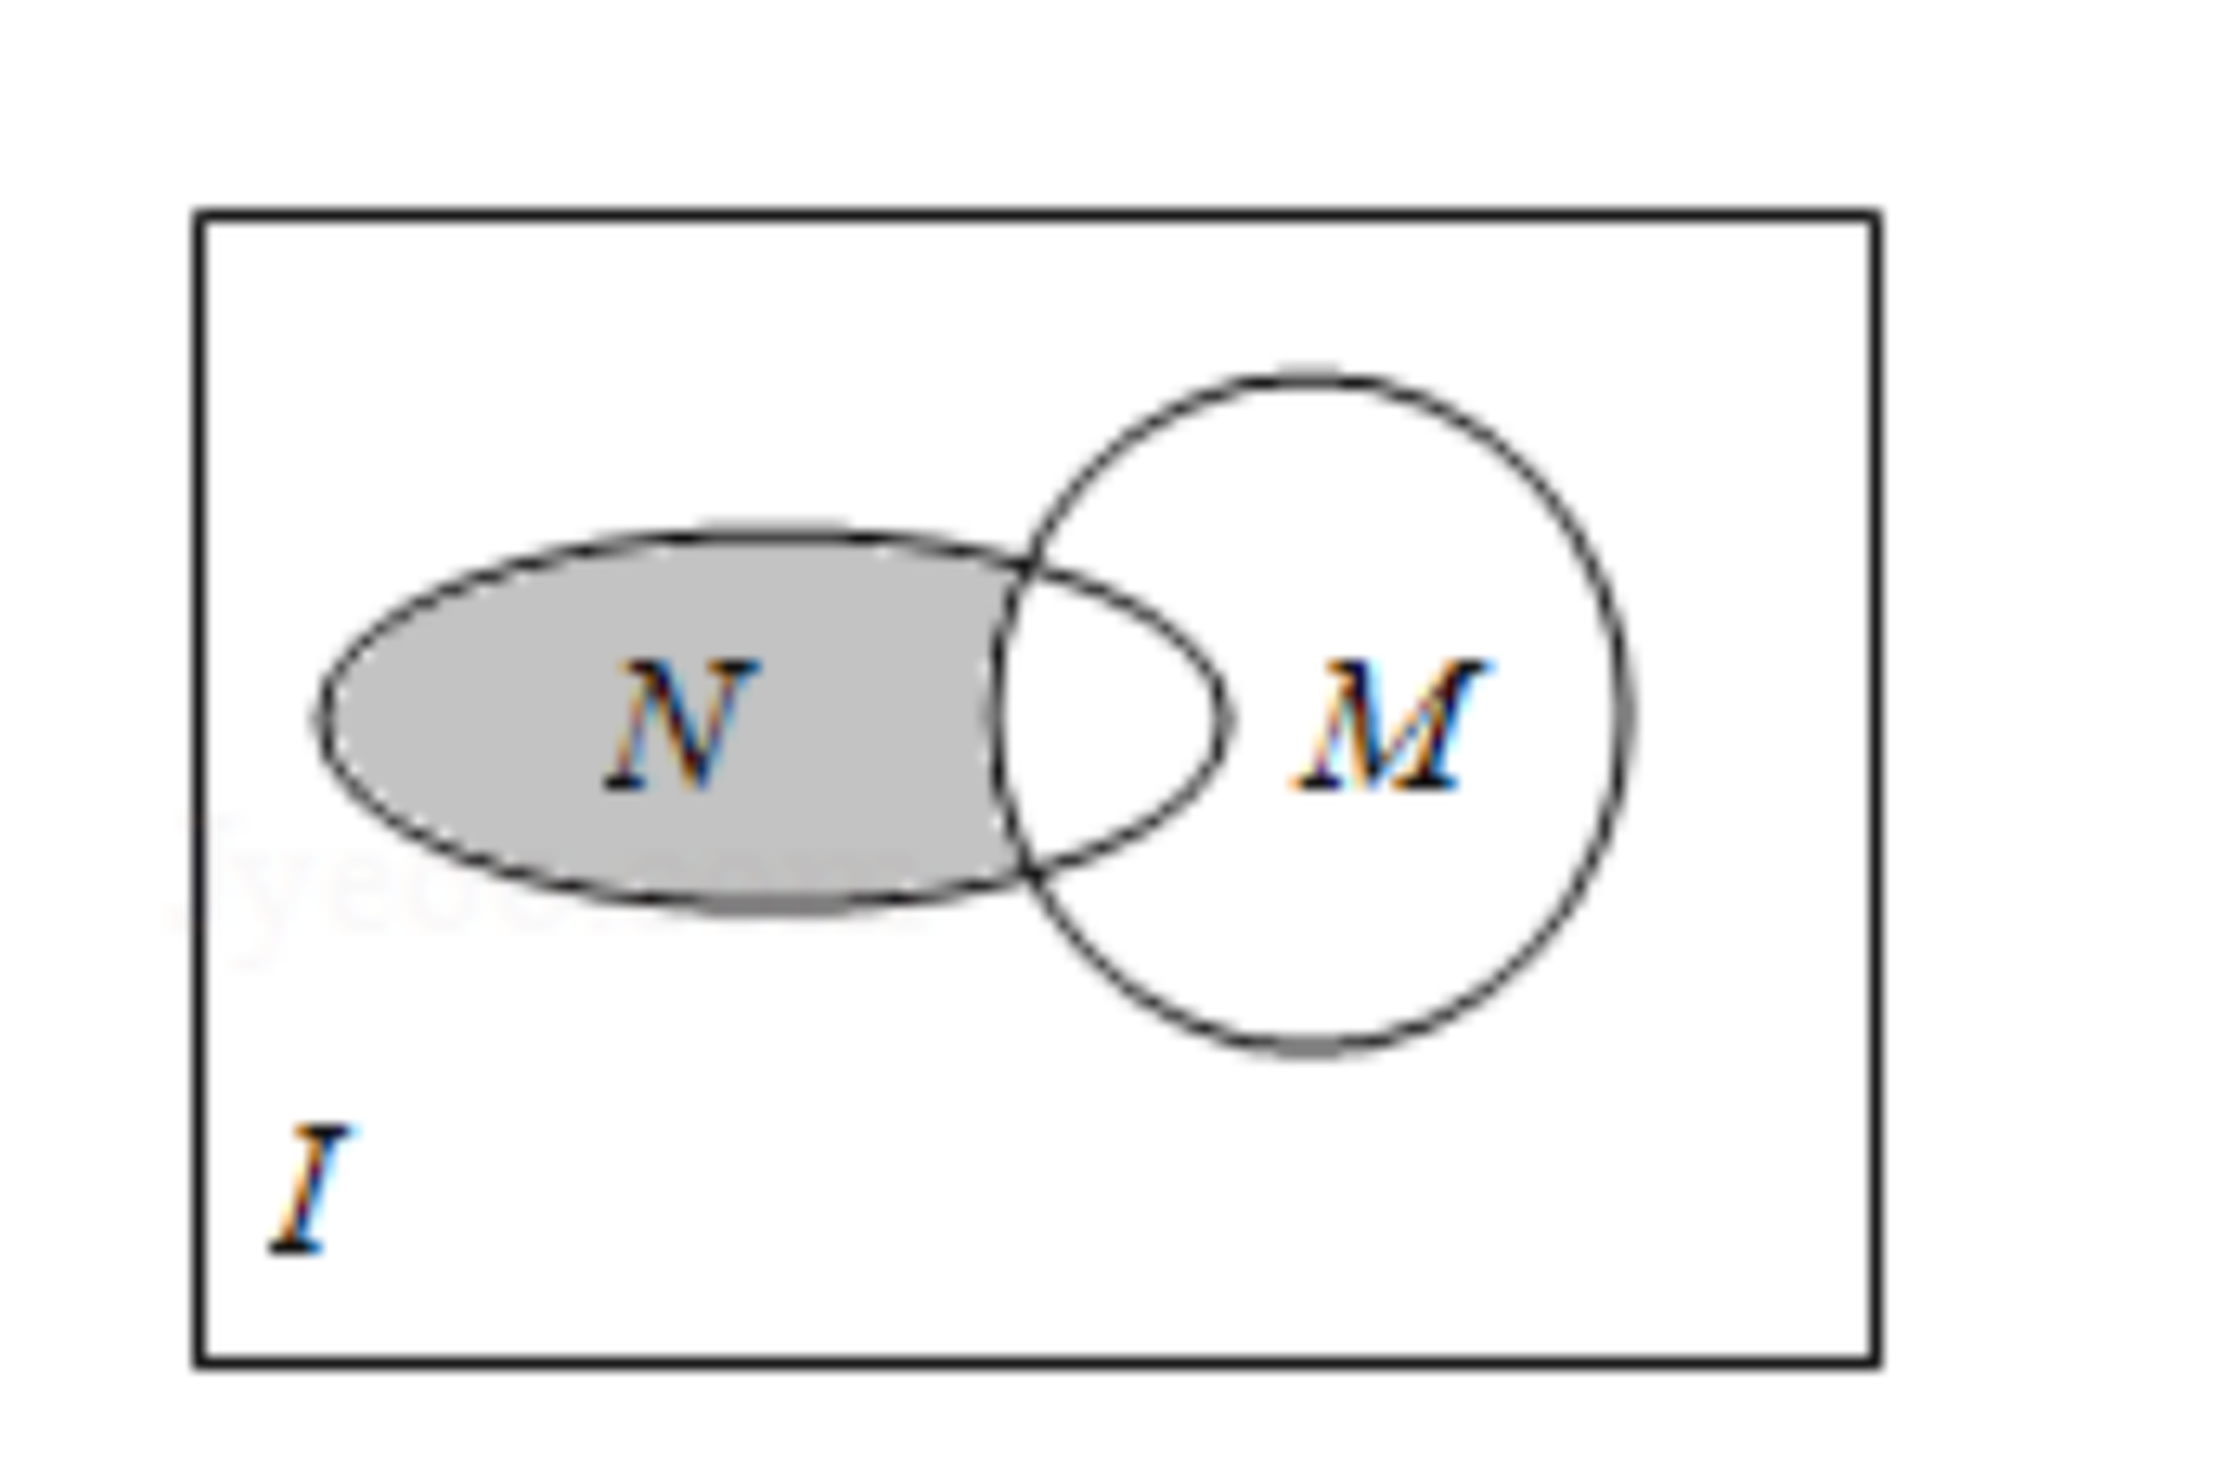
\includegraphics[width=0.30\textwidth]{figures/venn_N_cap_CI_M_h39.png}
\end{center}

\ans{$[-3,-\sqrt3)$}

\ifanswer
\solbegin
\step{阴影部分用集合表示为 $N\cap(\complement_UM)$.}
\step{则 $M=\{x\mid y=\sqrt{3-x^2}\}=\{x\mid3-x^2\geqslant0\}=\{x\mid-\sqrt3\leqslant x\leqslant\sqrt3\}$，}
\step{则 $\complement_UM=\{x\mid x>\sqrt3\text{ 或 }x<-\sqrt3\}$，$N=\{x\mid|x+1|\leqslant2\}=\{x\mid-3\leqslant x\leqslant1\}$，}
\step{则 $N\cap(\complement_UM)=\{x\mid-3\leqslant x<-\sqrt3\}$.}
\solend

\fi

\item 已知 $f(x)=x^2+ax+b$，集合 $\{x\mid f(x)=x\}=\{4\}$，将集合 $M=\{x\mid f(x)=4\}$ 用列举法表示 \blankline[4.4em].

\ans{$\{3,4\}$}

\ifanswer
\solbegin
\step{已知 $f(x)=x^2+ax+b$，集合 $\{x\mid f(x)=x\}=\{4\}$，}
% 注：原卷本行作「…$x^2+(a-1)x+b=0$ **由**两个相等的实数根为 $4$」——「由」当为「有」
%     （「设…是…有」的杂糅）；本稿照录未改，见文件头「原卷笔误/存疑」⑧。
\step{即方程 $x^2+ax+b=x$，$x^2+(a-1)x+b=0$ 由两个相等的实数根为 $4$，}
\step{所以 $\triangle=(a-1)^2-4b=0$，即 $x^2+(a-1)x+b=(x-4)^2$，所以 $b=16$，$a=-7$，}
\step{所以 $f(x)=x^2+ax+b=x^2-7x+16$，所以集合 $M=\{x\mid f(x)=4\}$，}
\step{即 $x^2-7x+16=4$，$x^2-7x+12=0$，故 $M=\{x\mid f(x)=4\}=\{3,4\}$.}
\solend

\fi

% 注：原卷方程组第二式印作 $1-2<-k\leqslant3$，按其结论 $-3\leqslant k<2$ 反推疑当作 $-2<-k\leqslant3$，
%     照录未改，见文件头「笔误/存疑」③。
\item 关于 $x$ 的不等式组 $\begin{cases}x^2-x-2>0\\ 2x^2+(2k+5)x+5k<0\end{cases}$ 的整数解的集合为 $\{-2\}$，
则实数 $k$ 的取值范围 \blankline[4.4em].

\ans{$-3\leqslant k<2$}

\ifanswer
\solbegin
\step{原不等式组即 $\begin{cases}(x-2)(x+1)>0\\ (x+k)(2x+5)<0\end{cases}$，整数解的集合为 $A$，若 $A=\{-2\}$，}
\step{则 $(-2+k)(2\times(-2)+5)<0$，所以 $k<2$，且有 $\begin{cases}-k>-\dfrac52\\ 1-2<-k\leqslant3\end{cases}$，}
\step{解得 $-3\leqslant k<2$.}
\solend

\fi

\item 规定 $\oplus$ 与 $\otimes$ 是两个运算符号，其运算法则如下，对任意实数 $a$、$b$ 有：$a\otimes b=ab$，
$a\oplus b=b(a^2+b^2+1)$. 若 $-2<a<b<2$ 且 $a$、$b\in\Z$，
$A=\left\{x\mid x=2(a\otimes b)+\dfrac{a\oplus b}{2b}\right\}$，则用列举法表示集合 $A=$ \blankline[4.4em].

\ans{$\left\{1,-\dfrac12\right\}$}

\ifanswer
\solbegin
\step{$A=\left\{x\mid x=2(a\otimes b)+\dfrac{a\oplus b}{2b}\right\}
=\left\{x\mid x=2ab+\dfrac{b(a^2+b^2+1)}{2b}\right\}$}
\step{$=\left\{x\mid x=2ab+\dfrac12a^2+\dfrac12b^2+\dfrac12\right\}
=\left\{x\mid x=\dfrac12(a+b)^2+ab+\dfrac12\right\}$，}
% 注：题设含 $\dfrac{a\oplus b}{2b}$，而 $-2<a<b<2$、$a$、$b\in\Z$ 时 $(a,b)=(-1,0)$ 也合条件、
%     却使分母 $2b=0$；原卷解析仍代入该组并约去 $b$ 得 $x=1$（答案集恰好不变）。本稿照录，
%     见文件头「原卷笔误/存疑」⑨。
\step{当 $a=-1$，$b=0$ 时，$x=1$；当 $a=-1$，$b=1$ 时，$x=-\dfrac12$；}
\step{当 $a=0$，$b=1$ 时，$x=1$；所以 $A=\left\{1,-\dfrac12\right\}$.}
\solend

\fi

\item 高斯是德国著名的数学家，近代数学奠基者之一，享有“数学王子”的称号，为了纪念数学家高斯，
我们把取整函数 $y=[x]$，$x\in\R$ 称为高斯函数，其中 $[x]$ 表示不超过 $x$ 的最大整数，
如 $[1.1]=1$，$[-1.1]=-2$. 则点集 $P=\{(x,y)\mid[x]^2+[y]^2=1\}$
所表示的平面区域的面积是 \blankline[4.4em].

\ans{$4$}

\ifanswer
\solbegin
\step{$[x]^2+[y]^2=1$ 由 $\begin{cases}[x]=0\\ [y]=-1\end{cases}$ 或 $\begin{cases}[x]=0\\ [y]=1\end{cases}$
或 $\begin{cases}[x]=-1\\ [y]=0\end{cases}$ 或 $\begin{cases}[x]=1\\ [y]=0\end{cases}$ 四个平面区域组成，}
\step{即 $\begin{cases}0\leqslant x<1\\ -1\leqslant y<0\end{cases}$ 或 $\begin{cases}0\leqslant x<1\\ 1\leqslant y<2\end{cases}$
或 $\begin{cases}-1\leqslant x<0\\ 0\leqslant y<1\end{cases}$ 或 $\begin{cases}1\leqslant x<2\\ 0\leqslant y<1\end{cases}$，}
\step{作出平面区域如图所示，平面区域由四个边长为 $1$ 的正方形组成，}
% 图在【解析】内（仅答案版出），取原卷截图（03.png，2560×3620）中部，4× LANCZOS 放大。
\begin{center}
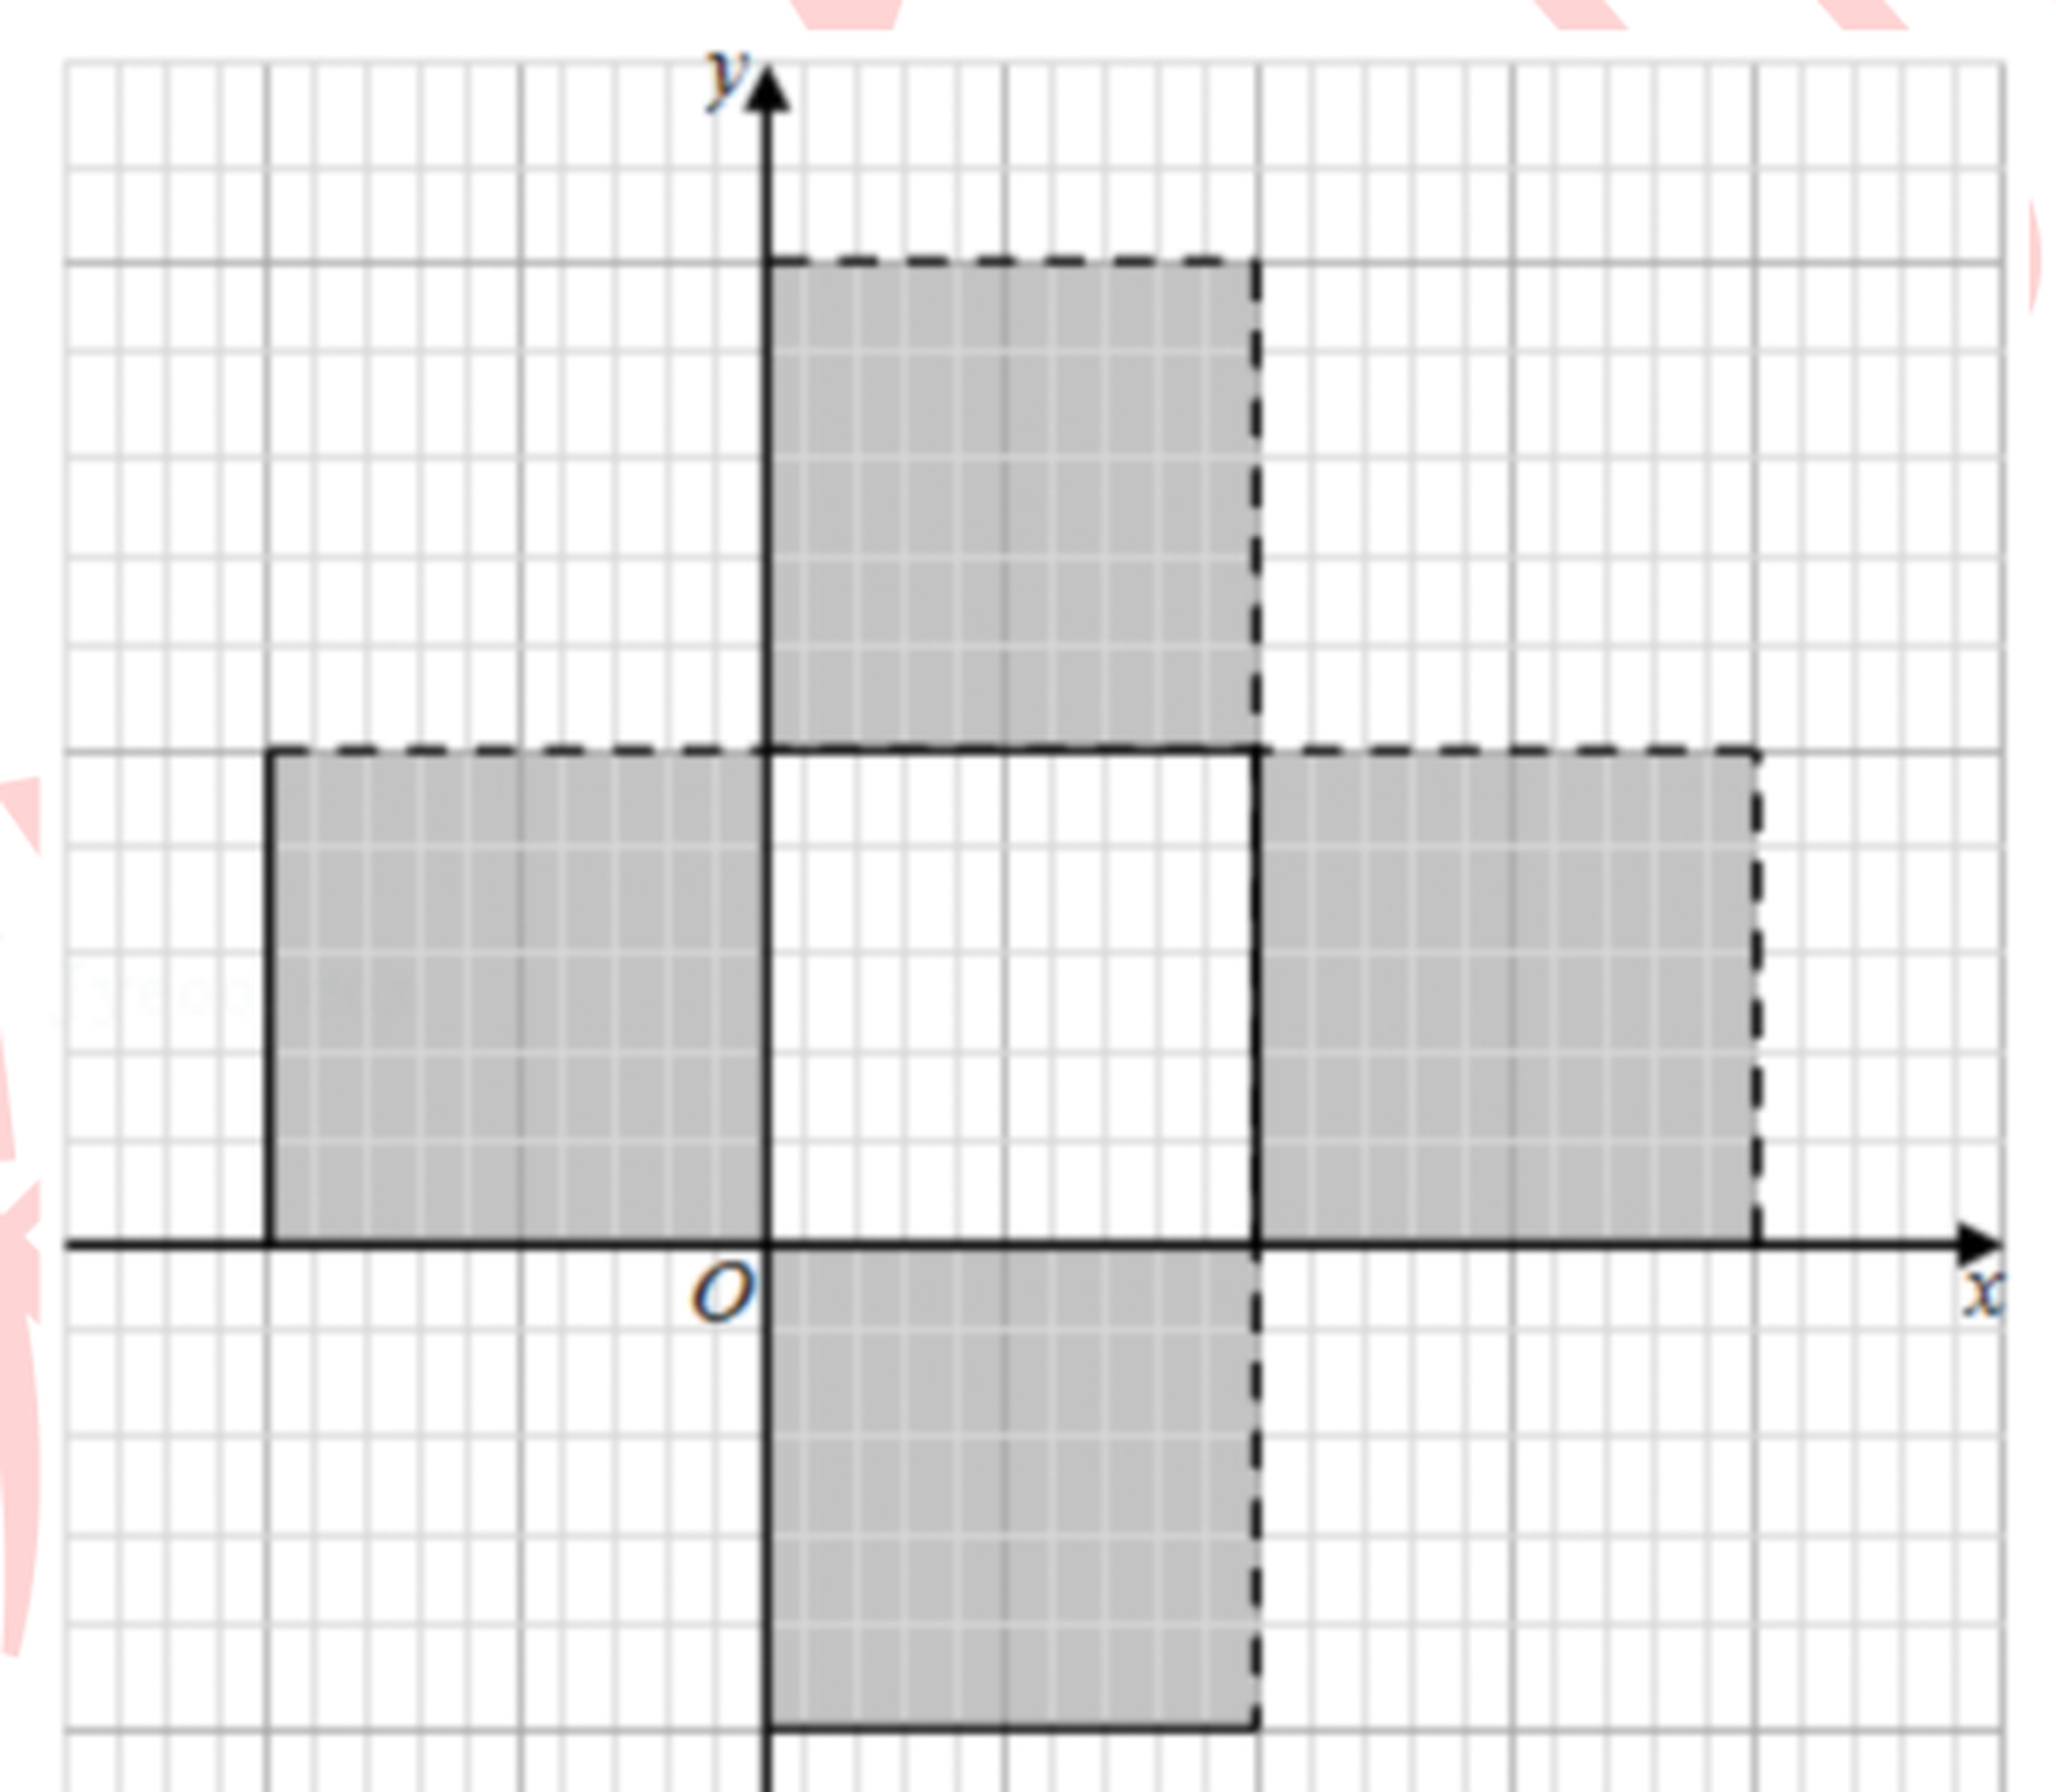
\includegraphics[width=0.38\textwidth]{figures/plane_grid_4squares_h39.png}
\end{center}
\step{总面积为 $1\times4=4$.}
\solend

\fi

\item 关于 $x$ 的不等式 $ax^2+bx+c>0$ 的解集为 $\{x\mid x<\beta\text{ 或 }x>\gamma\}(0<\beta<\gamma)$，
则不等式 $a(x^2+1)+b(x-1)+c>2ax$ 的解集为 \blankline[4.4em].

\ans{$(-\infty,\beta+1)\cup(\gamma+1,+\infty)$}

\ifanswer
\solbegin
\step{由题意得 $\beta$、$\gamma$ 为方程 $ax^2+bx+c=0$ 的两根且 $a>0$，}
\step{则 $\beta+\gamma=-\dfrac ba$，$\beta\gamma=\dfrac ca$，故 $b=-a(\beta+\gamma)$，$c=\beta\gamma a$，}
\step{则不等式可化为 $a(x^2+1)-a(\beta+\gamma)(x-1)+\beta\gamma a>2ax$，}
\step{因为 $a>0$，所以 $x^2+1-(\beta+\gamma)(x-1)+\beta\gamma>2x$，}
\step{即 $x^2-(\beta+\gamma+2)x+(\beta+\gamma+\beta\gamma+1)>0$，所以 $(x-\beta-1)(x-\gamma-1)>0$，}
\step{解得 $x<\beta+1$ 或 $x>\gamma+1$，所以不等式解集为 $(-\infty,\beta+1)\cup(\gamma+1,+\infty)$.}
\solend

\fi

\end{enumerate}

\bigsec{二、选择题}

\begin{enumerate}
\setcounter{enumi}{12}

\item 设 $a<b<0$，则下列不等式中不成立的是\mbox{（\quad）}

\keepwithprev
A. $\dfrac1a>\dfrac1b$\qquad B. $\dfrac{1}{a-b}>\dfrac1a$\qquad C. $|a|>-b$\qquad D. $\sqrt{-a}>\sqrt{-b}$

\ans{$B$}

\ifanswer
\solbegin
\step{令 $a=-2$，$b=-1$，}
\step{A、$-\dfrac12>-1$，正确；B、$-1<-\dfrac12$，故 B 错误；C、$2>1$，正确；}
\step{D、$\sqrt2>1$，正确；故选 B.}
\solend

\fi

\item 设实数集 $\R$ 为全集，集合 $P=\{x\mid f(x)=0\}$，$Q=\{x\mid g(x)=0\}$，$H=\{x\mid h(x)=0\}$，
则方程 $\dfrac{f^2(x)+g^2(x)}{h(x)}=0$ 的解集是\mbox{（\quad）}

\keepwithprev
A. $P\cap Q\cap\overline{H}$\qquad B. $P\cap Q$\qquad C. $P\cap Q\cap H$\qquad D. $P\cap Q\cup H$

\ans{$A$}

\ifanswer
\solbegin
\step{方程 $\dfrac{f^2(x)+g^2(x)}{h(x)}=0$ 等价于 $\begin{cases}f(x)=0\\ g(x)=0\\ h(x)\neq0\end{cases}$，}
\step{又因为 $P=\{x\mid f(x)=0\}$，$Q=\{x\mid g(x)=0\}$，$H=\{x\mid h(x)=0\}$，}
\step{所以方程 $\dfrac{f^2(x)+g^2(x)}{h(x)}=0$ 的解集是 $P\cap Q\cap\overline{H}$，故选 A.}
\solend

\fi

\item 设全集 $U$，在下列条件中，是 $B\sub A$ 的充要条件的有\mbox{（\quad）}

\keepwithprev
% 注：原卷此行 ② 与 ③ 之间**漏排分隔号**（①、③ 后都有「；」，② 后没有）；
%     本稿照录未补，见文件头「原卷笔误/存疑」⑩。
①$A\cup B=A$；\qquad ②$\overline{A}\cap B=\varnothing$\qquad ③$\overline{A}\sub\overline{B}$；\qquad ④$A\cup\overline{B}=U$

\keepwithprev
A. $1$ 个\qquad B. $2$ 个\qquad C. $3$ 个\qquad D. $4$ 个

\ans{$D$}

\item 已知集合 $M=\{x\mid x\in\N,0<x\leqslant15\}$，$A_1$、$A_2$、$A_3$ 满足：①$A_1\cup A_2\cup A_3=M$；
②每个集合都恰有 $5$ 个元素. 集合 $A_i(i=1,2,3)$ 中最大元素与最小元素之和称为 $A_i$ 的特征数，
记为 $X_i(i=1,2,3)$，则 $X_1+X_2+X_3$ 的值不可能为\mbox{（\quad）}

\keepwithprev
A. $37$\qquad B. $39$\qquad C. $48$\qquad D. $57$

\ans{$A$}

\ifanswer
\solbegin
\step{因为集合 $M=\{x\mid x\in\N,0<x\leqslant15\}=\{1,2,3,\cdots,15\}$，}
\step{又因为集合 $A_1$、$A_2$、$A_3$ 中，每个集合恰有 $5$ 个元素，}
\step{且 $A_1\cup A_2\cup A_3=M$ 有 $15$ 个元素，所以集合 $A_1$、$A_2$、$A_3$ 中没有重复元素，}
\step{因为 $1$ 是集合 $M$ 中数值最小的元素，$15$ 是集合 $M$ 中数值最大的元素，}
\step{所以在 $A_i$ 的特征数构成中，必有 $1$ 和 $15$，不妨设 $1\in A_1$，$15\in A_1$，}
% 注：原卷本行（与下面「最小」那句）在「集合」后的角标是**数字 $1$**（同句 $X_1$ 的角标同形），
%     而非上一行「$A_i$ 的特征数构成」里的斜体 $A_i$——原卷两种下标并存，本稿照录、不归一，
%     见文件头「原卷笔误/存疑」⑬。
\step{要使 $X_1+X_2+X_3$ 最大，则应该在集合 $A_1$ 中首先放置数值较小的元素，}
\step{即 $A_1=\{1,2,3,4,15\}$，所以 $5$ 与 $14$ 是剩下元素中数值最小或最大的元素，}
\step{同理，不妨设 $5\in A_2$，$14\in A_2$，接着在 $A_2$ 中再次放置数值较小的元素，}
\step{即 $A_2=\{5,6,7,8,14\}$，则 $A_3=\{9,10,11,12,13\}$，}
\step{此时 $X_1+X_2+X_3$ 有最大值为 $1+15+5+14+9+13=57$，}
\step{即 $X_1+X_2+X_3\leqslant57$；}
% 注：同上一处——原卷此行角标是**数字 $1$**（$A_1$），本稿照录，未与「$A_i$」归一。
\step{要使 $X_1+X_2+X_3$ 最小，则在集合 $A_1$ 中首先放置数值较大的元素，}
\step{即 $A_1=\{1,12,13,14,15\}$，所以 $2$ 与 $11$ 是剩下元素中数值最小或最大的元素，}
\step{同理，不妨设 $2\in A_2$，$11\in A_2$，接着在 $A_2$ 中再次放置数值较大的元素，}
\step{即 $A_2=\{2,8,9,10,11\}$，则 $A_3=\{3,4,5,6,7\}$，}
\step{此时 $X_1+X_2+X_3$ 有最小值为 $1+15+2+11+3+7=39$，}
\step{即 $X_1+X_2+X_3\geqslant39$，}
\step{综上，$39\leqslant X_1+X_2+X_3\leqslant57$，故选 A.}
\solend

\fi

\end{enumerate}

\bigsec{三、解答题}

\begin{enumerate}
\setcounter{enumi}{16}

% 注：原卷首句「由数 $y=-x^2+ax-1=-x+3$」中的「由数」显系「由」或「由函数」之误；末段
%     的两处分类讨论与结论自相矛盾（详见文件头「笔误/存疑」④）。本稿一律照录，未改。
\item 命题 $p$：函数 $y=-x^2+ax-1$ 与 $y=-x+3$ 图象交点的横坐标均为负值，
命题 $q$：关于 $x$ 的方程 $2(1-x)a+(x^2-10x-3)=0$ 的两个根，一个大于 $3$，另一个小于 $3$；
若命题 $p$ 和命题 $q$ 中有且仅有一个是真命题，求 $a$ 的取值范围.

\ans{$\R$}

\ifanswer
\solbegin
\step{由数 $y=-x^2+ax-1=-x+3$ 得 $x^2-(a+1)x+4=0$，}
\step{若横坐标均为负值，则满足 $\begin{cases}\Delta=(a+1)^2-16\geqslant0\\ x_1x_2=4>0\\ x_1+x_2=a+1<0\end{cases}$
得 $\begin{cases}a\geqslant3\text{ 或 }a\leqslant-5\\ a<-1\end{cases}$，得 $a\leqslant-5$，}
\step{即 $p:a\leqslant-5$，}
\step{若方程 $2(1-x)a+(x^2-10x-3)=0$ 的两个根，一个大于 $3$，另一个小于 $3$；}
\step{设 $f(x)=2(1-x)a+(x^2-10x-3)$，则 $f(3)<0$，即 $-4a-24<0$，}
\step{得 $a>-6$，即 $q:a>-6$，}
\step{因为命题 $p$ 和命题 $q$ 中有且仅有一个是真命题，}
\step{若 $p$ 真 $q$ 假，则 $\begin{cases}a\leqslant-5\\ a>-6\end{cases}$，得 $a\in\R$，}
\step{若 $p$ 假 $q$ 真，则 $\begin{cases}a>-5\\ a\leqslant-6\end{cases}$，此时 $a$ 无解，}
\step{综上，实数 $a$ 的取值范围是 $\R$.}
\solend

\fi

\ansspace[8]

\item 设全集是实数集 $\R$，$A=\left\{x\mid\dfrac{1-2x}{x-3}\geqslant0\right\}$，$B=\{x\mid x^2+a\leqslant0\}$.

\begin{enumerate}[label=(\arabic*)]

\item 当 $a=-4$ 时，求 $A\cup B$；

\item 若 $\overline{A}\cap B=B$，求实数 $a$ 的取值范围.

\end{enumerate}

\ans{（1）$\{x\mid-2\leqslant x<3\}$；（2）$\left(-\dfrac14,+\infty\right)$}

\ifanswer
\solbegin
\stepm{(1)}{$A=\left\{x\mid\dfrac{1-2x}{x-3}\geqslant0\right\}=\left\{x\mid\dfrac12\leqslant x<3\right\}$，$B=\{x\mid x^2+a\leqslant0\}$.}
\step{当 $a=-4$ 时，$B=\{x\mid-2\leqslant x\leqslant2\}$，所以 $A\cup B=\{x\mid-2\leqslant x<3\}$.}
\stepm{(2)}{$\overline{A}=\left\{x\mid x\geqslant3\text{ 或 }x<\dfrac12\right\}$，$B=\{x\mid x^2+a\leqslant0\}$.}
\step{由 $\overline{A}\cap B=B$，得 $B\sub\overline{A}$，}
\step{则当 $a>0$ 时，$B=\varnothing$，满足 $B\sub\overline{A}$，则 $a>0$ 成立，}
\step{则当 $a=0$ 时，$B=\{0\}$，满足 $B\sub\overline{A}$，则 $a=0$ 成立，}
\step{当 $a<0$ 时，$B=\{x\mid-\sqrt{-a}\leqslant x<\sqrt{-a}\}$，}
\step{得 $\sqrt{-a}<\dfrac12$，即 $-\dfrac14<a<0$，}
\step{综上，实数 $a$ 的取值范围是 $\left(-\dfrac14,+\infty\right)$.}
\solend

\fi

\ansspace[6]

\item 设集合 $A=\{x\mid ax^2+2x+1=0,a\in\R\}$.

\begin{enumerate}[label=(\arabic*)]

\item 当 $A$ 中元素个数为 $1$ 时，求：$a$ 和 $A$；

\item 当 $A$ 中元素个数至少为 $1$ 时，求：$a$ 的取值范围；

\item 求：$A$ 中各元素之和.

\end{enumerate}

\ans{（1）$a=0$ 时 $A=\left\{-\dfrac12\right\}$，$a=1$ 时 $A=\{-1\}$；（2）$(-\infty,1]$；
（3）$a=0$ 时和为 $-\dfrac12$，$a<1$ 且 $a\neq0$ 时和为 $-\dfrac2a$，$a=1$ 时和为 $-1$，$a>1$ 时 $A$ 中无元素}

\ifanswer
\solbegin
\stepm{(1)}{集合 $A=\{x\mid ax^2+2x+1=0,a\in\R\}$，$A$ 中元素个数为 $1$，}
\step{所以 $a=0$ 或 $\begin{cases}a\neq0\\ \Delta=4-4a=0\end{cases}$，解得 $a=0$，$A=\left\{-\dfrac12\right\}$ 或 $a=1$，$A=\{-1\}$.}
\stepm{(2)}{当 $A$ 中元素个数至少为 $1$ 时，$a=0$ 或 $\begin{cases}a\neq0\\ \Delta=4-4a\geqslant0\end{cases}$，解得 $a\leqslant1$，}
\step{所以 $a$ 的取值范围是 $(-\infty,1]$.}
\stepm{(3)}{当 $a=0$ 时，$A$ 中元素之和为 $-\dfrac12$；}
\step{当 $a<1$ 且 $a\neq0$ 时，$A$ 中元素之和为 $-\dfrac2a$；}
\step{当 $a=1$ 时，$A$ 中元素之和为 $-1$；}
\step{当 $a>1$ 时，$A$ 中无元素.}
\solend

\fi

\ansspace[8]

\item 设 $k$ 是正整数，集合 $A$ 至少有两个元素，且 $A\sub\N^*$. 如果对于 $A$ 中的任意两个不同的
元素 $x$、$y$，都有 $|x-y|\neq k$，则称 $A$ 具有性质 $P(k)$.

\begin{enumerate}[label=(\arabic*)]

\item 试判断集合 $B=\{1,2,3,4\}$ 和 $C=\{1,4,7,10\}$ 是否具有性质 $P(2)$？并说明理由；

\item 若集合 $A=\{a_1,a_2,\cdots,a_{12}\}\sub\{1,2,\cdots,20\}$，求证：$A$ 不可能具有性质 $P(3)$；

\item 若集合 $A\sub\{1,2,\cdots,2023\}$，且同时具有性质 $P(4)$ 和 $P(7)$，求集合 $A$ 中元素个数的
最大值.

\end{enumerate}

\ans{（1）$B$ 不具有性质 $P(2)$，$C$ 具有性质 $P(2)$；（2）见解析；（3）$920$}

\ifanswer
\solbegin
\stepm{(1)}{因为 $B=\{1,2,3,4\}$，}
\step{又 $1\in\N^*$，$2\in\N^*$，$3\in\N^*$，$4\in\N^*$，但 $|4-2|=2$，}
\step{所以集合 $B$ 不具有性质 $P(2)$，}
\step{因为 $C=\{1,4,7,10\}$，}
\step{又 $1\in\N^*$，$4\in\N^*$，$7\in\N^*$，$10\in\N^*$，}
\step{但 $|4-1|=3$，$|7-1|=6$，$|10-1|=9$，$|7-4|=3$，$|10-4|=6$，$|10-7|=3$，}
\step{所以集合 $C$ 具有性质 $P(2)$，}
\stepm{(2)}{将集合 $\{1,2,\cdots,20\}$ 中的元素分为如下 $11$ 个集合，}
% 注：原卷本行 $\{8,11\}$ 与 $\{9,12\}$ 之间的分隔号误用**句号**「.」（同行其余处皆逗号），
%     本稿照录、未改，见文件头「原卷笔误/存疑」⑪。
\step{$\{1,4\}$，$\{2,5\}$，$\{3,6\}$，$\{7,10\}$，$\{8,11\}$.$\{9,12\}$，$\{13,16\}$，$\{14,17\}$，$\{15,18\}$，}
\step{$\{19\}$，$\{20\}$，}
\step{所以从集合 $\{1,2,\cdots,20\}$ 中取 $12$ 个元素，则前 $9$ 个集合至少要选 $10$ 个元素，}
\step{所以必有 $2$ 个元素取自前 $9$ 个集合中的同一集合，即存在两个元素其差为 $3$，}
\step{所以 $A$ 不可能具有性质 $P(3)$；}
\stepm{(3)}{先说明连续 $11$ 项中集合 $A$ 中最多选取 $5$ 项，}
\step{以 $1,2,3,\cdots,11$ 为例.}
\step{构造抽屉 $\{1,8\}$，$\{2,9\}$，$\{3,10\}$，$\{4,11\}$，$\{5\}$，$\{6\}$，$\{7\}$.}
\step{①$5$、$6$、$7$ 同时选，因为具有性质 $P(4)$ 和 $P(7)$，}
\step{所以选 $5$ 则不选 $1$、$9$；选 $6$ 则不选 $2$、$10$；选 $7$ 则不选 $3$、$11$；}
% 注：原卷此步推理不严——「只剩 $4$、$8$」但两数相差 $4$、不能同选，该情形实际最多只能取 $4$ 个；
%     末句「不超过 $5$ 个」的结论仍成立。本稿照录，见文件头「原卷笔误/存疑」⑫。
\step{则只剩 $4$、$8$；故 $1,2,3,\cdots,11$ 中属于集合 $A$ 的元素个数不超过 $5$ 个.}
\step{②$5$、$6$、$7$ 选 $2$ 个，}
\step{若只选 $5$、$6$，则 $1$、$2$、$9$、$10$、$7$ 不可选，又 $\{4,11\}$ 只能选一个元素，}
\step{$3$、$8$ 可以选，故 $1,2,3,\cdots,11$ 中属于集合 $A$ 的元素个数不超过 $5$ 个.}
\step{若选 $5$、$7$，则只能从 $2$、$4$、$8$、$10$ 中选，但 $4$、$8$ 不能同时选，}
\step{故 $1,2,3,\cdots,11$ 中属于集合 $A$ 的元素个数不超过 $5$ 个.}
\step{若选 $6$、$7$，则 $2$、$3$、$10$、$11$、$5$ 不可选，又 $\{1,8\}$ 只能选一个元素，}
\step{$4$、$9$ 可以选，故 $1,2,3,\cdots,11$ 中属于集合 $A$ 的元素个数不超过 $5$ 个.}
\step{③$5$、$6$、$7$ 中只选 $1$ 个，}
\step{又四个集合 $\{1,8\}$，$\{2,9\}$，$\{3,10\}$，$\{4,11\}$ 每个集合至多选 $1$ 个元素，}
\step{故 $1,2,3,\cdots,11$ 中属于集合 $A$ 的元素个数不超过 $5$ 个.}
\step{由上述①②③得，连续 $11$ 项自然数中属于集合 $A$ 的元素至多只有 $5$ 个，}
\step{如取 $1$、$4$、$6$、$7$、$9$.}
\step{因为 $2023=183\times11+10$，则把每 $11$ 个连续自然数分组，}
\step{前 $183$ 组每组至多选取 $5$ 项；}
\step{从 $2014$ 开始，最后 $10$ 个数至多选取 $5$ 项，}
\step{故集合 $A$ 的元素最多有 $184\times5=920$ 个.}
\step{给出如下选取方法：从 $1,2,3,\cdots,11$ 中选取 $1$、$4$、$6$、$7$、$9$；}
\step{然后在这 $5$ 个数的基础上每次累加 $11$，构造 $183$ 次.}
\step{此时集合 $A$ 的元素为 $1$，$4$，$6$，$7$，$9$；$12$，$15$，$17$，$18$，$20$；$23$，$26$，$28$，$29$，$31$；
$\cdots$；$2014$，$2017$，$2019$，$2020$，$2022$，共 $920$ 个元素.}
\step{经检验得该集合符合要求，故集合 $A$ 的元素最多有 $920$ 个.}
\solend

\fi

\ansspace[10]

\end{enumerate}

\bigsec{附加题}

\begin{enumerate}
\setcounter{enumi}{20}

\item 若规定集合 $M=\{a_1,a_2,\cdots,a_n\}$（$n\in\N^*$）的子集 $\{a_{i_1},a_{i_2},\cdots,a_{i_m}\}$（$m\in\N^*$）
为 $M$ 的第 $k$ 个子集，其中 $k=2^{i_1-1}+2^{i_2-1}+\cdots+2^{i_m-1}$，则 $M$ 的第 $25$ 个子集是 \blankline[4.4em].

\ans{$\{a_1,a_4,a_5\}$}

\ifanswer
\solbegin
\step{由题意得 $M$ 的第 $k$ 个子集，且 $k=2^{i_1-1}+2^{i_2-1}+\cdots+2^{i_m-1}$，}
\step{又 $25=2^0+2^3+2^4=2^{1-1}+2^{4-1}+2^{5-1}$，所以 $M$ 的第 $25$ 个子集是 $\{a_1,a_4,a_5\}$.}
\solend

\fi

% 注：原卷在 $x=1$、$y=2$、$z=3$ 时把 $B=\{x,y\}$ 印作 $\{1,3\}$（应为 $\{1,2\}$），
%     照录未改，见文件头「笔误/存疑」⑥。
\item 用 $|S|$ 表示集合 $S$ 中的元素的个数，设 $A$、$B$、$C$ 为集合，称 $(A,B,C)$ 为有序三元组.
如果集合 $A$、$B$、$C$ 满足 $|A\cap B|=|B\cap C|=|C\cap A|=1$，且 $A\cap B\cap C=\varnothing$，
则称有序三元组 $(A,B,C)$ 为最小相交. 由集合 $\{1,2,3\}$ 的子集构成的所有有序三元组中，
最小相交的有序三元组的个数为 \blankline[4.4em].

\ans{$6$}

\ifanswer
\solbegin
\step{因为 $|A\cap B|=|B\cap C|=|C\cap A|=1$，}
\step{所以设 $A\cap B=\{x\}$，$B\cap C=\{y\}$，$C\cap A=\{z\}$，}
% 图在【解析】内（仅答案版出），取原卷截图（10.png，2560×3620）右栏，4× LANCZOS 放大。
\begin{center}
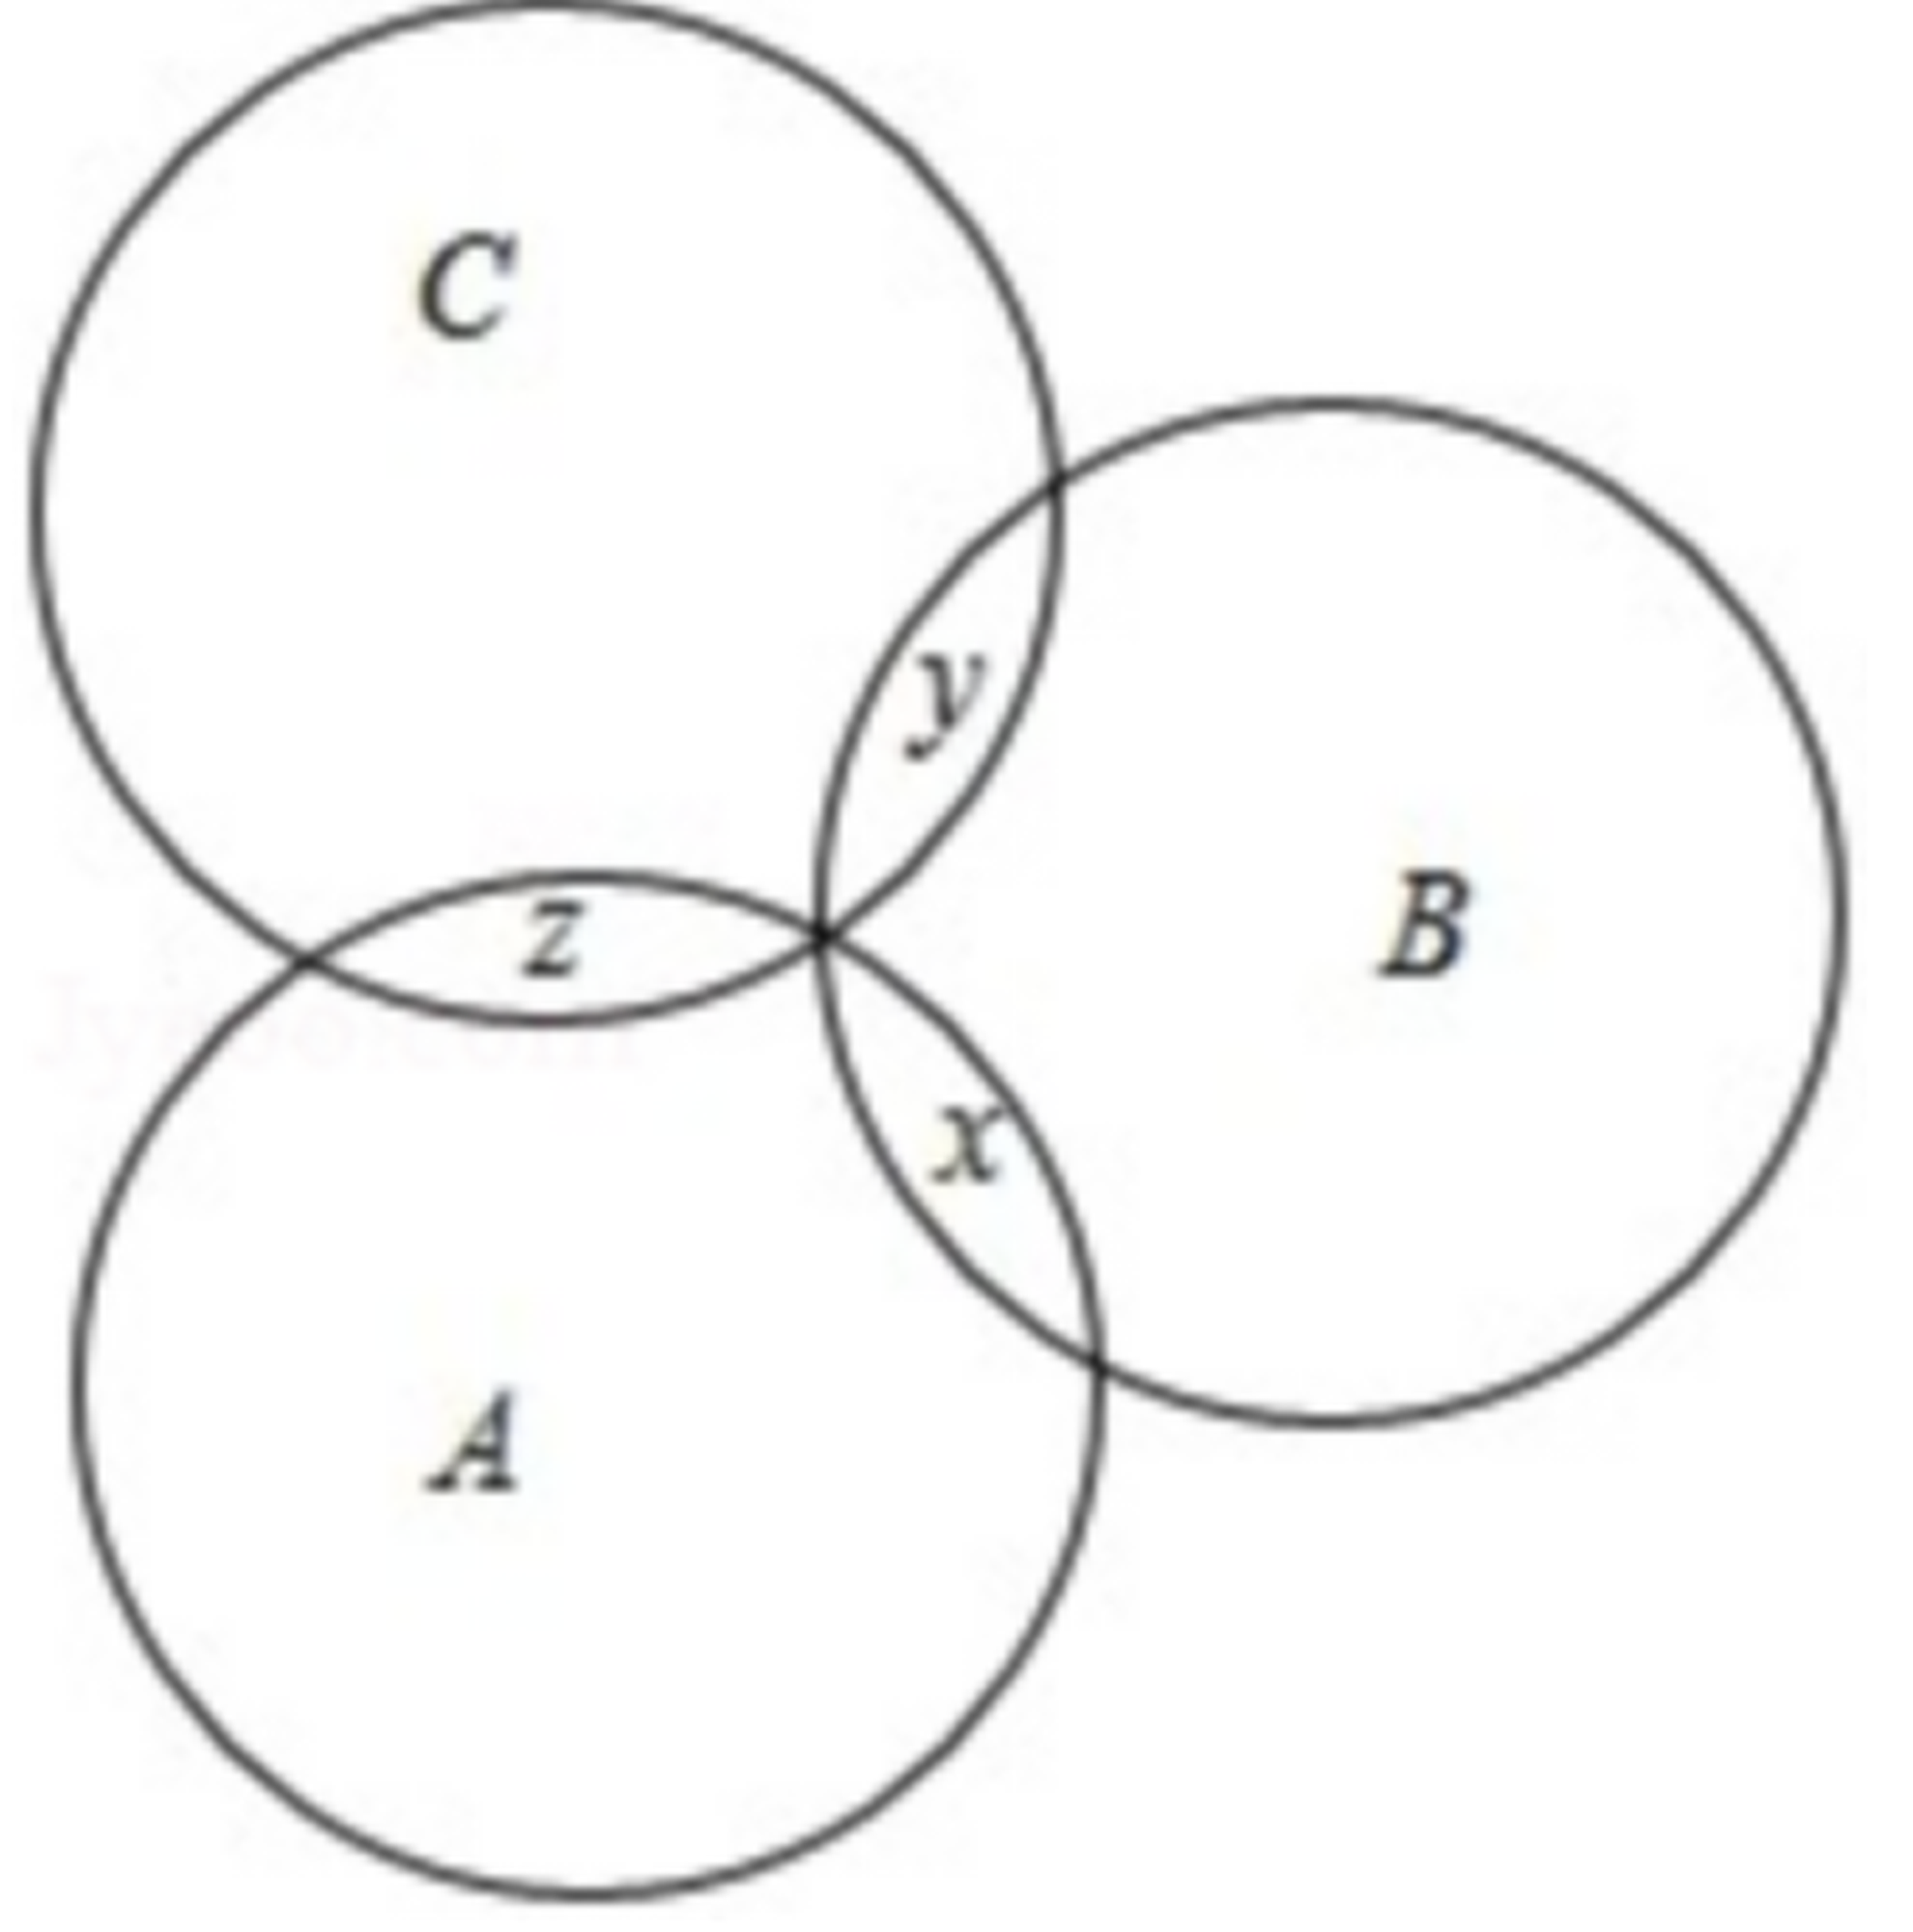
\includegraphics[width=0.30\textwidth]{figures/venn_ABC_x_y_z_h39.png}
\end{center}
\step{因为 $|A\cap B|=|B\cap C|=|C\cap A|=1$，且 $x$、$y$、$z\in\{1,2,3\}$，}
\step{所以集合 $A=\{x,z\}$，$B=\{x,y\}$，$C=\{z,y\}$，}
\step{若 $x=1$，$y=2$，$z=3$，则 $A=\{1,3\}$，$B=\{1,3\}$，$C=\{2,3\}$，}
\step{将 $1$，$2$，$3$ 进行全排列，有 $P_3^3=3\times2=6$ 个.}
\solend

\fi

\item 已知集合 $T=\{1,2,\cdots,2025\}$，对于 $T$ 的每一个非空子集的所有元素，计算它们乘积的倒数，
则所有这样倒数的和为 \blankline[4.4em].

\ans{$2025$}

\ifanswer
\solbegin
\step{集合 $T=\{1,2,\cdots,2025\}$ 的非空子集的个数为 $2^{2025}-1$，}
\step{这些子集中，每个元素的乘积分别为}
\step{$1,2,3,\cdots,2025,1\times2,1\times3,\cdots,1\times2025,\cdots,1\times2\times3\times\cdots\times2025$，}
\step{每项都可以看作是从 $1,2,3,\cdots,2025$ 中选择若干项的乘积，}
\step{$1+\dfrac12+\cdots+\dfrac{1}{2025}+\dfrac{1}{1\times2}+\dfrac{1}{1\times3}+\cdots+\dfrac{1}{2024\times2025}
+\cdots+\dfrac{1}{1\times2\times\cdots\times2025}$}
\step{$=(1+1)\left(1+\dfrac12\right)\cdots\left(1+\dfrac{1}{2025}\right)-1
=2\times\dfrac32\times\dfrac43\times\cdots\times\dfrac{2026}{2025}-1=2025$.}
\solend

\fi

% 第 24 题是压轴题，题干较长；试卷版在它之前量一次页高，尽量不与前文分家（照全稿成例）。
\ansneed{5cm}
% 注：原卷【解析】①③ 两步把 $f(x)$ 印作 $f[x[x]]$，显系笔误，照录未改，见文件头「笔误/存疑」⑦。
\item 若 $X$ 是一个集合，$T$ 是一个以 $X$ 的某些子集为元素的集合，且满足：①$X$ 属于 $T$，
$\varnothing$ 属于 $T$；②$T$ 中任意多个元素的并集属于 $T$；③$T$ 中任意多个元素的交集属于 $T$.
则称 $T$ 是集合 $X$ 上的一个拓扑. 已知函数 $f(x)=[x[x]]$，其中 $[x]$ 表示不大于 $x$ 的最大整数，
当 $x\in(0,n]$，$n\in\N^*$ 时，函数 $f(x)$ 值域为集合 $A_n$，则集合 $A_2$ 上的含有 $4$ 个元素的
拓扑 $T$ 的个数为 \blankline[4.4em].

\ans{$9$}

\ifanswer
\solbegin
\step{由题意，$n=2$，故 $0<x\leqslant2$，}
\step{①当 $0<x<1$ 时，则 $[x]=0$，所以 $f[x[x]]=0$，}
\step{②当 $x=1$ 时，$[x]=1$ 显然 $f(1)=1$，}
\step{③当 $1<x<2$ 时，$[x]=1$，所以 $f[x[x]]=[x]=1$，}
\step{④当 $x=2$ 时，$f(2)=4$，}
\step{所以 $A_2=\{0,1,4\}$，}
\step{因为 $T$ 中含有 $4$ 个元素，其中两个元素 $\varnothing$ 和 $A_2$，}
\step{$A_2=\{0,1,4\}$. 其它两个元素为 $A$、$B$，则
$\begin{cases}A\neq\varnothing\\ A\neq A_2\\ B\neq\varnothing\\ B\neq A_2\\ A\neq B\end{cases}$，}
\step{由对称性，不妨设 $1\leqslant|A|\leqslant|B|\leqslant2$，其中 $|A|$、$|B|$ 表示集合 $A$ 中元素的个数，}
\step{因为 $\begin{cases}A\cap B\in T\\ A\cup B\in T\end{cases}$，又 $|A|\leqslant|B|$，所以 $A\cap B=\varnothing$ 或 $A$，}
\step{若 $A\cap B=\varnothing$，则 $A\cup B$ 只能等于 $A_2$，}
\step{（若 $A\cup B=B$，则 $A\sub B$，则 $A\cap B=A=\varnothing$，矛盾）}
\step{则必有 $\begin{cases}|A|=1\\ |B|=2\end{cases}$，所以 $(A,B)$ 的个数 $\Leftrightarrow$ $A$ 的个数 $=3$ 种，}
\step{即 $\begin{cases}A=\{0\}\\ B=\{1,4\}\end{cases}$ 或 $\begin{cases}A=\{1\}\\ B=\{0,4\}\end{cases}$
或 $\begin{cases}A=\{4\}\\ B=\{0,1\}\end{cases}$；}
\step{若 $A\cap B=A\Leftrightarrow A\sub B$ 此时满足 $A\cup B=B$，}
\step{因为 $A\neq B$ 且 $1\leqslant|A|$ 且 $|B|\leqslant2$，所以 $\begin{cases}|A|=1\\ |B|=2\end{cases}$，}
\step{所以 $B$ 的选择共有 $C_3^2=3$ 种，则 $A$ 的个数有 $C_2^1$ 种，}
\step{所以 $(A,B)$ 的个数 $=2\times3=6$ 种.}
% 这六组「$A$／$B$」按原卷排作两行（前五个一行、第六个另起一行）；因五组并排时
% amsmath 的 cases 会为每组的第二列各留一枚 \quad，本行改排 \left\{\begin{matrix}…\end{matrix}\right.
% 以省下这枚 \quad（照 README「说明」记的高一07 成例），字形与 cases 相同。
\step{（这 $6$ 种是 $\left\{\begin{matrix}A=\{0\}\\ B=\{0,1\}\end{matrix}\right.$、
$\left\{\begin{matrix}A=\{1\}\\ B=\{0,1\}\end{matrix}\right.$、
$\left\{\begin{matrix}A=\{0\}\\ B=\{0,4\}\end{matrix}\right.$、
$\left\{\begin{matrix}A=\{4\}\\ B=\{0,4\}\end{matrix}\right.$、
$\left\{\begin{matrix}A=\{1\}\\ B=\{1,4\}\end{matrix}\right.$、}
\step{$\left\{\begin{matrix}A=\{4\}\\ B=\{1,4\}\end{matrix}\right.$）.}
\step{综上，$T$ 的个数为 $9$ 个.}
\solend

\fi

\end{enumerate}

\end{document}
"
% 紧凑版：xelatex "\def\iscompact{1}% 高一39_大同中学_周末作业4.1.tex
%   —— 高一上数学「2026-2027 年大同中学高一上周末作业 4.1」（试卷版/答案版）
% 试卷版：xelatex 高一39_大同中学_周末作业4.1.tex
% 答案版：xelatex "\def\isanswer{1}\input{高一39_大同中学_周末作业4.1.tex}"
% 紧凑版：xelatex "\def\iscompact{1}\input{高一39_大同中学_周末作业4.1.tex}"
%
% 原始材料是微信公众号图文（公众号「魔都数学加油站」连载「27学年高一 39」，署名「破晓」，
% 2026-09-26 21:29 发布，原文标题「27学年高一39——2026-2027年上海市大同中学高一上周末作业4.1」，
% 原文链接 https://mp.weixin.qq.com/s/HR2hIayXUXNi4zTs3PioiQ ），正文为 11 张 PNG 页。**同一篇里各页分辨率不一致**（2560×3620 与 4762×6735 两档混排：第 1、3、8、10 页为
% 2560×3620，第 2、4、5、6、7、9、11 页为 4762×6735）。原文本身就是一份**讲评版**——除第 15 题
% 外各题题下直接印【解析】（无单独的【答案】行），第 15 题的答案「D」直接印在题干末尾的括号内。
% 试题文字、答案与解析均照原卷录入，未改内容。卷面的粉色斜水印「魔都数学加油站」属水印，未录入。
%
% 卷首标题：原卷页首印作「2026-2027 年大同中学高一上周末作业 4.1」（**卷面标题行即带校名**，
% 年份区间按全稿惯例排 en dash，前缀照原卷保留「年」）。
%
% 篇幅与题号：卷面自「一、填空题」的**第 3 题**起编，终于「附加题」的**第 24 题**，共 22 题
% （填空 3—12、选择 13—16、解答 17—20、附加题 21—24）。第 1、2 题未在该文中发布——这是该
% 公众号连载讲评版的通例（高一02—高一09 等均自第 3 题起编，README「说明」已记），**不是截断**，
% 故本稿题号亦自 3 起。它与 高一40（大同中学 周末作业4.2）同属「周末作业 4」系列但**各自独立起编**
% （4.2 自第 3 题起、终于第 19 题），不是同一份试卷的两半。
%
% 与原卷的排版差异（均已在 README「说明」中交代）：
%   ① 原文自**第 3 题**起（第 1、2 题未在该文中发布），故本稿题号亦自 3 起，填空题以
%      \setcounter{enumi}{2} 起编；选择、解答、附加题三节各按上一节末号另设 \setcounter
%      （选择题 \setcounter{enumi}{12}、解答题 \setcounter{enumi}{16}、附加题 \setcounter{enumi}{20}）；
%   ② 原卷本就印有「一、填空题」「二、选择题」「三、解答题」三节标题，末节印作「附加题」
%      （**不带「四、」**，且题号 21—24 续前编、不另起），本稿照原卷分节，只把标题改排成全稿
%      统一的「大节标题」样式；
%   ③ 原卷是「讲评版」：除第 15 题外，各题题下均印【解析】（**全卷无一条独立的【答案】行**）；
%      第 15 题无解析，答案「D」直接印在题干末尾的括号内。本稿统一改为试卷版隐去、答案版以
%      \ans{}／\ifanswer 块给出，两版彻底分离；原卷写在【解析】末句的结果，本稿照 高一38
%      （同校同系列、同为讲评版）的成例另提为 \ans{}；
%   ④ 数集记号原卷两套并用：实数集作斜体的 $R$（第 7、11、14、17、18、19 题），整数集作斜体
%      $Z$（第 10 题），自然数集作斜体 $N$ 及 $N^*$（第 16、20、21、24 题），本稿按全稿惯例
%      统一写作 $\R$、$\Z$、$\N$、$\N^*$；
%   ⑤ 补集符号原卷两套并用：第 7 题作前缀式的 $C_U$（且题干称全集为 $I$，见「笔误/存疑」①），
%      第 14、15、18 题作上横线（$\overline{H}$、$\overline{A}$、$\overline{B}$），本稿照录、不归一
%      （前缀式写作 $\complement_U$，与 高一c／高一10 的成例一致）；
%   ⑥ 包含符号原卷两套并用：第 3 题作**无下划线**的 $\subset$，第 15、18、20、24 题作**带下划线**
%      的 $\sub$，本稿照录、不归一；
%   ⑦ 原卷填空的横线约两个字宽，本稿按全稿惯例统一排 \blankline[4.4em]；
%   ⑧ 第 7、11、22 题各有插图，取原卷截图、4× LANCZOS 放大（figures/venn_N_cap_CI_M_h39.png、
%      figures/plane_grid_4squares_h39.png、figures/venn_ABC_x_y_z_h39.png）；第 7 题的 Venn 属
%      **题干**（试卷版、答案版都出），第 11、22 题的图在【解析】内（仅答案版出）。第 7 题图
%      左下、第 11 题图的上／左／右边缘带进极淡的原卷粉色水印残影——照全稿「插图直接取自
%      原卷截图、不用 TikZ 重绘、不修图」的体例保留（再裁会切到坐标轴与 $x$、$y$、$O$ 标注）；
%   ⑨ 原卷并列的字母、数字（「$x_1,x_2$」「$a,b$」「$1,2,3,\cdots,11$」）多作半角逗号或不加标点，
%      本稿按全稿惯例改排顿号（$x_1$、$x_2$）或把数列并入行内公式；半角括号、逗号一律排全角，
%      数学式内部的标点照原样；
%   ⑩ 原卷未印副标题，本稿按**本卷实际内容**补出副标题「集合与常用逻辑用语」（依据见下条）。
%
% 副标题（\examtitlest 第二个参数）：本卷卷面未印副标题，由本稿补出，取值按 2026-09-26 起的
%   新口径「只用本卷实际内容的模块名」定为「集合与常用逻辑用语」。依据：全卷 22 题（第 3—24 题）中，
%   第 3、5、7、8、10、11、14、15、16、17、18、19、20、21、22、23、24 题共 17 题是集合的运算与
%   关系、子集／真子集、补集、集合新定义（「全食／偏食」、最小相交、拓扑、特征数）与集合计数，
%   以及命题与常用逻辑用语（第 3 题充要条件、第 5 题存在量词命题、第 17 题命题真假）；其余两题
%   第 4、6 考一元二次方程的根（韦达定理）与方程恒等，第 9、12、13 题是不等式（一元二次不等式组
%   的整数解、一元二次不等式解集、不等式的性质）——不等式合计 3/22，**不足全卷三分之一**，
%   故不并标「不等式」。
%
% 原卷笔误/存疑（均照抄原卷、未改，见源码中该处上方注释）：
%   ① 第 7 题题干称「全集 $I=R$」，而【解析】两处把补集写作 $C_U M$（下标作 $U$），前后记号不一；
%      本稿照录，未改；
%   ② 第 4 题【解析】两处把判别式印作 $\triangle=[2(m-1)^2-16m^2]$（方括号内首项漏了平方，
%      正确应作 $[2(m-1)]^2-16m^2$）；按其所判「$m=\frac12$ 时 $<0$、$m=-\frac12$ 时 $>0$」反推，
%      $[2(m-1)]^2-16m^2$ 在 $m=\frac12$ 时为 $-3<0$、在 $m=-\frac12$ 时为 $5>0$，与结论一致；
%      本稿照录；
%   ③ 第 9 题【解析】把方程组第二式印作 $1-2<-k\leqslant3$，按其结论 $-3\leqslant k<2$ 反推，
%      疑当作 $-2<-k\leqslant3$（原卷多一个「$1$」）；本稿照录；
%   ④ 第 17 题【解析】首句「由数 $y=-x^2+ax-1=-x+3$」中的「由数」显系「由」或「由函数」之误；
%      且末段「若 $p$ 真 $q$ 假…得 $a\in R$」「若 $p$ 假 $q$ 真…此时 $a$ 无解」与结论「$a$ 的取值范围
%      是 $R$」自相矛盾（按 $p:a\leqslant-5$、$q:a>-6$，$p$ 真 $q$ 假应为 $a\leqslant-6$，$p$ 假 $q$ 真
%      应为 $a>-5$，合起来是 $a\leqslant-6$ 或 $a>-5$，并非 $R$）；本稿一律照录，未按正确解法改写；
%   ⑤ 第 18 题【解析】(2) 把 $B=\{x\mid x^2+a\leqslant0\}$（$a<0$）印作右端开的
%      $\{x\mid-\sqrt{-a}\leqslant x<\sqrt{-a}\}$（应为闭的「$\leqslant$」）；按其所判
%      $\sqrt{-a}<\frac12$ 反推，不影响结论；本稿照录；
%   ⑥ 第 22 题【解析】在 $x=1$、$y=2$、$z=3$ 时把 $B=\{x,y\}$ 印作 $\{1,3\}$（应为 $\{1,2\}$），
%      与本行前面「$B=\{x,y\}$」不合；本稿照录；
%   ⑦ 第 24 题【解析】①③ 两步把 $f(x)$ 印作 $f[x[x]]$，显系笔误；本稿照录。
%   ⑧ 第 8 题【解析】「即方程 $x^2+ax+b=x$，$x^2+(a-1)x+b=0$ **由**两个相等的实数根为 $4$」——
%      「由」当为「有」（「设…是…有」的杂糅）；本稿照录；
%   ⑨ 第 10 题：题设 $a\oplus b=b(a^2+b^2+1)$，而集合定义里含 $\dfrac{a\oplus b}{2b}$；$-2<a<b<2$、
%      $a$、$b\in\Z$ 时 $(a,b)=(-1,0)$ 也合条件、却使分母 $2b=0$，原卷解析仍代入该组并约去
%      $b$ 得 $x=1$（答案集恰好不变）；本稿照录；
%   ⑩ 第 15 题选项列里 ② 与 ③ 之间**漏排分隔号**（原卷作「② $\overline{A}\cap B=\varnothing$③
%      $\overline{A}\sub\overline{B}$；」——①、③ 后都有「；」，② 后没有）；本稿照录；
%   ⑪ 第 20(2) 把 $\{1,2,\cdots,20\}$ 分成的 11 个集合里，$\{8,11\}$ 与 $\{9,12\}$ 之间误用
%      **句号**「.」（同行其余处皆逗号）；本稿照录；
%   ⑫ 第 20(3)① 推理不严：原卷写「选 5 则不选 1、9；选 6 则不选 2、10；选 7 则不选 3、11；
%      则只剩 4、8」——但 4 与 8 相差 $4$、不能同选，该情形实际最多只能取 $4$ 个；末句结论
%      「不超过 $5$ 个」仍成立；本稿照录；
%   ⑬ 第 16 题【解析】两种下标并存：「所以在 $A_i$ 的特征数构成中」原卷作斜体 $A_i$，而
%      「要使 $X_1+X_2+X_3$ 最大（小），则（应）在集合 $A_1$ 中首先放置…」两处原卷作
%      **数字 $1$**（与同句 $X_1$ 的角标同形）；本稿照录、未归一。
%
% 图取原卷截图（依次见各处的 \includegraphics 前的注释），4× LANCZOS 放大。
\documentclass[a4paper,11pt]{article}
\usepackage{common}

\begin{document}

\examtitlest[3]{2026--2027 年大同中学高一上周末作业 4.1}{集合与常用逻辑用语}

\bigsec{一、填空题}

\begin{enumerate}
\setcounter{enumi}{2}

\item “$x\geqslant a$”是“$0<x<2$”的必要非充分条件，则实数 $a$ 的取值范围是 \blankline[4.4em].

\ans{$(-\infty,0]$}

\ifanswer
\solbegin
\step{因为 $x\geqslant a$ 是 $0<x<2$ 的必要非充分条件，所以 $(0,2)\subset[a,+\infty)$，所以 $a\leqslant0$，}
\step{则实数 $a$ 的取值范围是 $(-\infty,0]$.}
\solend

\fi

% 注：原卷$[2(m-1)^2-16m^2]$ 首项漏了平方（应为 $[2(m-1)]^2-16m^2$），照录未改，见文件头「笔误/存疑」②。
\item 若关于 $x$ 的方程 $x^2+2(m-1)x+4m^2=0$ 有两个实数根，且这两根互为倒数，则 $m=$ \blankline[4.4em].

\ans{$-\dfrac12$}

\ifanswer
\solbegin
\step{设 $x_1$、$x_2$ 是方程 $x^2+2(m-1)x+4m^2=0$ 有两个实数根，}
\step{则 $x_1x_2=4m^2=1$，解得 $m=\dfrac12$ 或 $m=-\dfrac12$，}
\step{又当 $m=\dfrac12$ 时，$\triangle=[2(m-1)^2-16m^2]<0$，舍去，}
\step{当 $m=-\dfrac12$ 时，$\triangle=[2(m-1)^2-16m^2]>0$，故 $m=-\dfrac12$.}
\solend

\fi

\item 已知命题：“存在 $x\in[1,2]$，使 $x^2+2x+a\geqslant0$”为真命题，则 $a$ 的取值范围是 \blankline[4.4em].

\ans{$a\geqslant-8$}

\ifanswer
\solbegin
\step{若存在 $x\in[1,2]$，使 $x^2+2x+a\geqslant0$，}
\step{则等价为存在 $x\in[1,2]$，使 $x^2+2x\geqslant-a$，}
\step{当存在 $x\in[1,2]$ 时，设 $y=x^2+2x=(x+1)^2-1$，则 $3\leqslant y\leqslant8$，}
\step{所以要使 $x^2+2x\geqslant-a$，则 $8\geqslant-a$，即 $a\geqslant-8$.}
\solend

\fi

\item 已知方程 $a(3x+2)+b(2x-3)=8x+3$ 有无穷多个解，则 $a:b=$ \blankline[4.4em].

\ans{$30:7$}

\ifanswer
\solbegin
\step{$a(3x+2)+b(2x-3)=(3a+2b)x+2a-3b=8x+3$ 有无穷多个解，}
\step{所以 $\begin{cases}3a+2b=8\\ 2a-3b=3\end{cases}$，解得 $a=\dfrac{30}{13}$，$b=\dfrac{7}{13}$，所以 $a:b=30:7$.}
\solend

\fi

% 注：原卷题干称「全集 $I=R$」，而【解析】两处把补集写作 $C_U M$（下标作 $U$），前后记号不一；
%     照录未改，见文件头「笔误/存疑」①。
\item 已知集合 $M=\{x\mid y=\sqrt{3-x^2}\}$，$N=\{x\mid-3\leqslant x\leqslant1\}$，全集 $I=\R$，
则图中阴影部分表示的集合为 \blankline[4.4em].

% 图取原卷截图（01.png，2560×3620）右栏，4× LANCZOS 放大。
\begin{center}
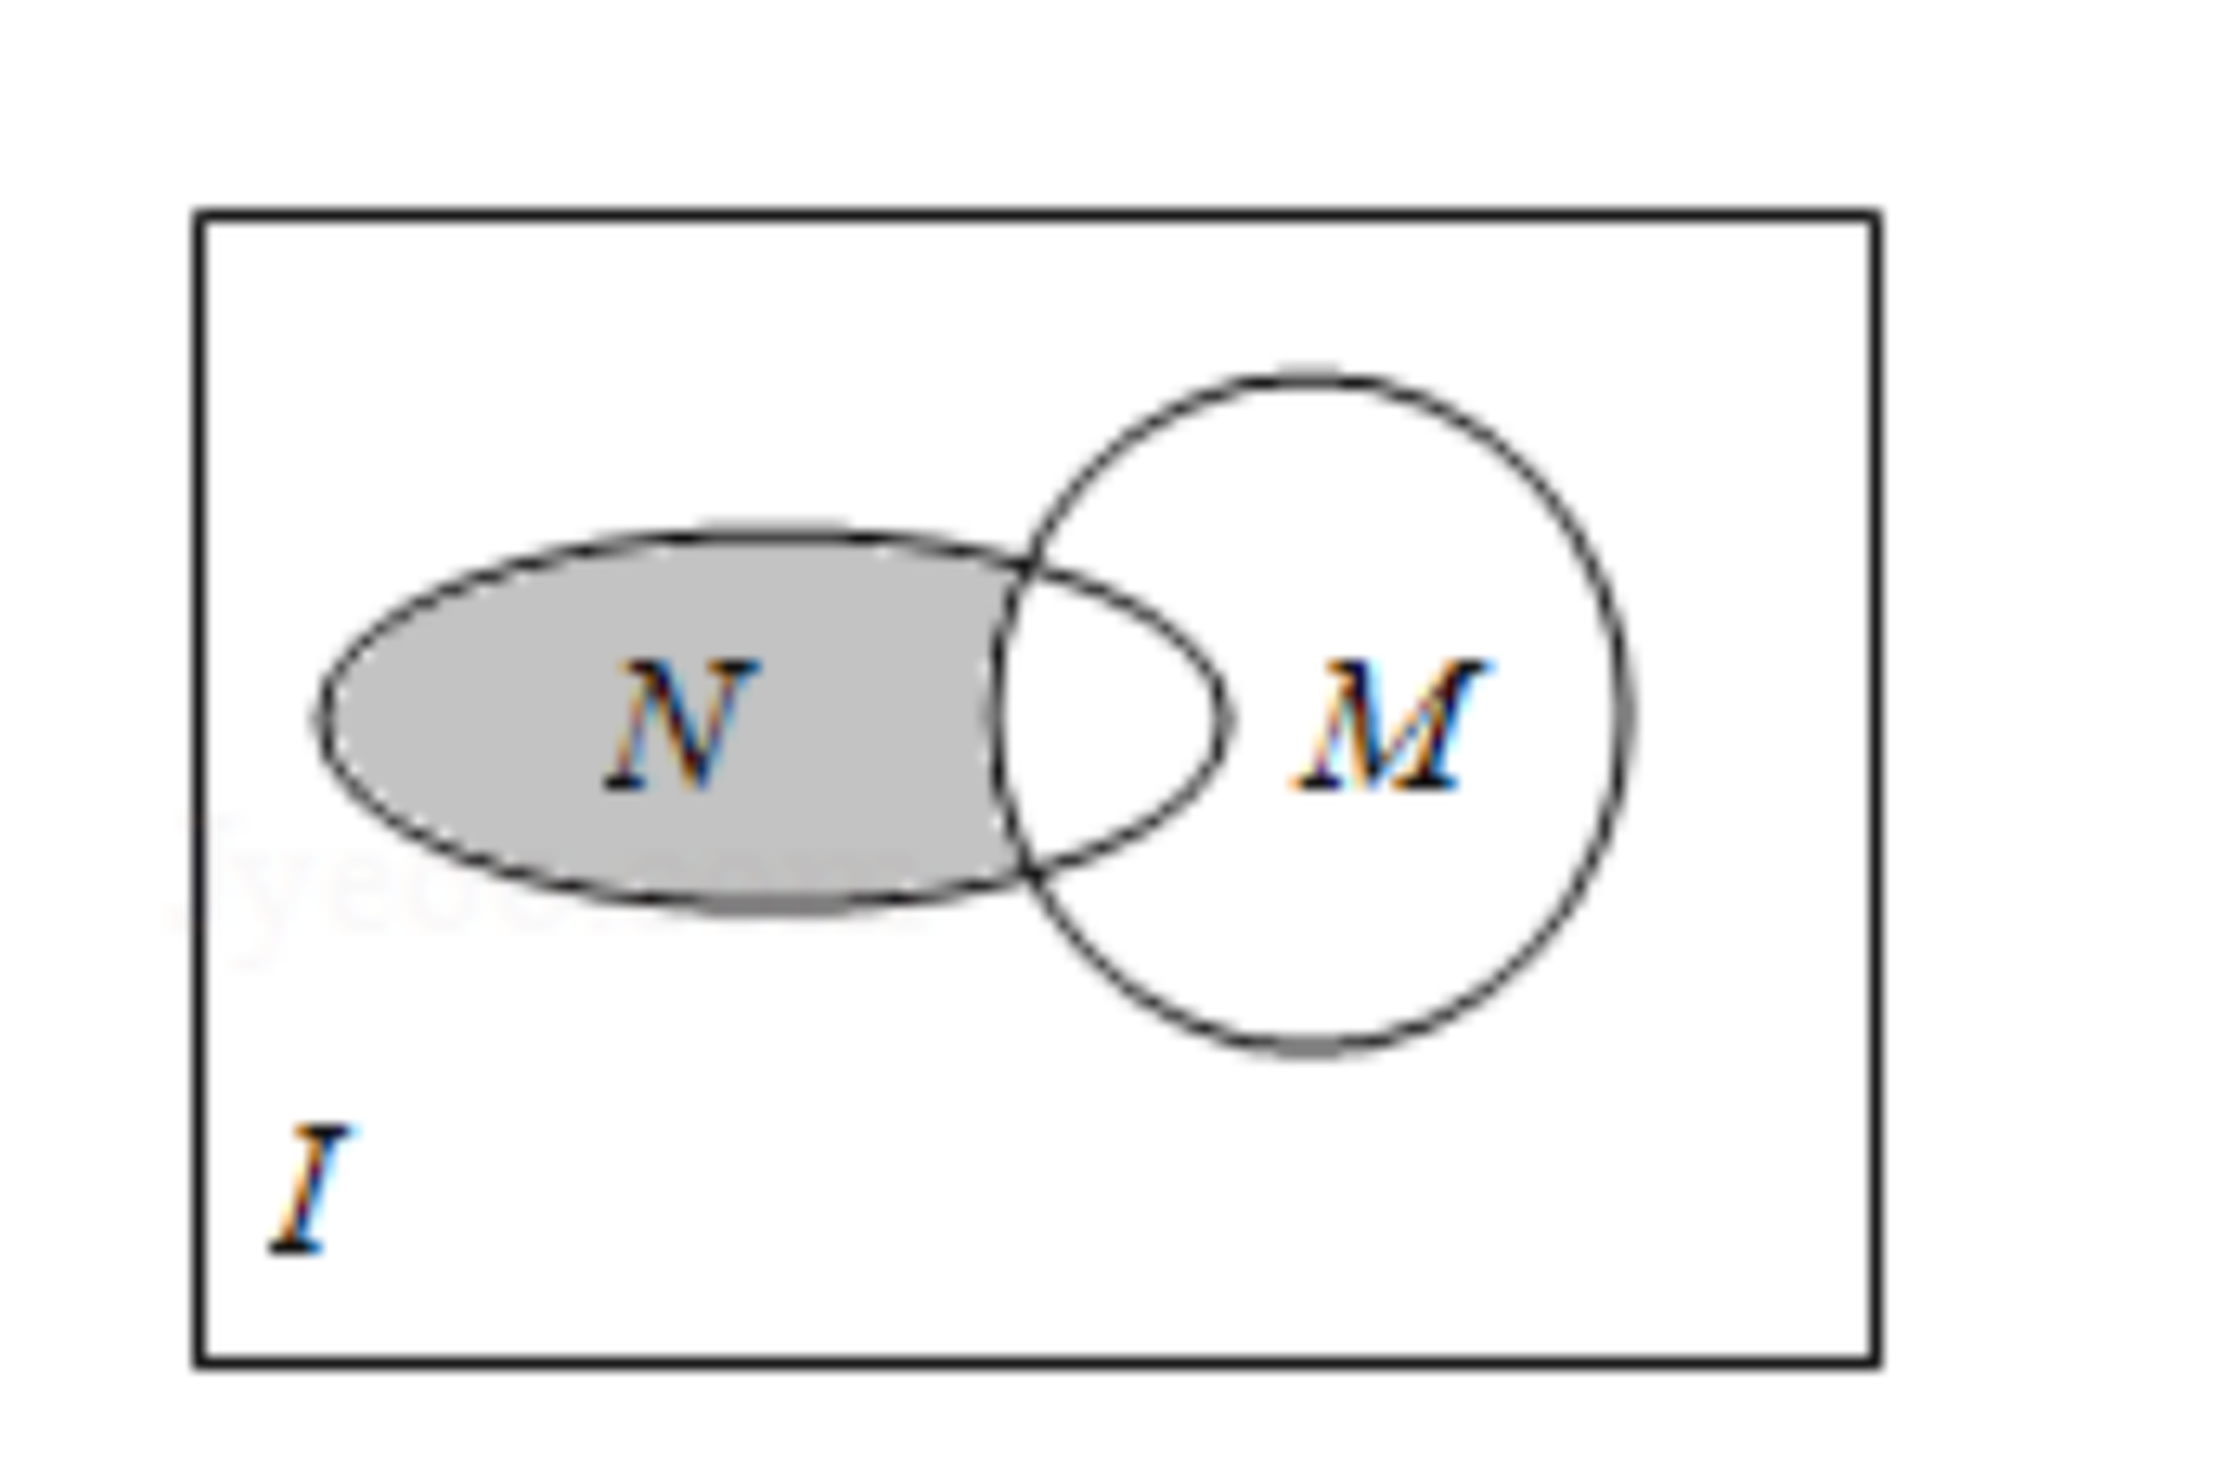
\includegraphics[width=0.30\textwidth]{figures/venn_N_cap_CI_M_h39.png}
\end{center}

\ans{$[-3,-\sqrt3)$}

\ifanswer
\solbegin
\step{阴影部分用集合表示为 $N\cap(\complement_UM)$.}
\step{则 $M=\{x\mid y=\sqrt{3-x^2}\}=\{x\mid3-x^2\geqslant0\}=\{x\mid-\sqrt3\leqslant x\leqslant\sqrt3\}$，}
\step{则 $\complement_UM=\{x\mid x>\sqrt3\text{ 或 }x<-\sqrt3\}$，$N=\{x\mid|x+1|\leqslant2\}=\{x\mid-3\leqslant x\leqslant1\}$，}
\step{则 $N\cap(\complement_UM)=\{x\mid-3\leqslant x<-\sqrt3\}$.}
\solend

\fi

\item 已知 $f(x)=x^2+ax+b$，集合 $\{x\mid f(x)=x\}=\{4\}$，将集合 $M=\{x\mid f(x)=4\}$ 用列举法表示 \blankline[4.4em].

\ans{$\{3,4\}$}

\ifanswer
\solbegin
\step{已知 $f(x)=x^2+ax+b$，集合 $\{x\mid f(x)=x\}=\{4\}$，}
% 注：原卷本行作「…$x^2+(a-1)x+b=0$ **由**两个相等的实数根为 $4$」——「由」当为「有」
%     （「设…是…有」的杂糅）；本稿照录未改，见文件头「原卷笔误/存疑」⑧。
\step{即方程 $x^2+ax+b=x$，$x^2+(a-1)x+b=0$ 由两个相等的实数根为 $4$，}
\step{所以 $\triangle=(a-1)^2-4b=0$，即 $x^2+(a-1)x+b=(x-4)^2$，所以 $b=16$，$a=-7$，}
\step{所以 $f(x)=x^2+ax+b=x^2-7x+16$，所以集合 $M=\{x\mid f(x)=4\}$，}
\step{即 $x^2-7x+16=4$，$x^2-7x+12=0$，故 $M=\{x\mid f(x)=4\}=\{3,4\}$.}
\solend

\fi

% 注：原卷方程组第二式印作 $1-2<-k\leqslant3$，按其结论 $-3\leqslant k<2$ 反推疑当作 $-2<-k\leqslant3$，
%     照录未改，见文件头「笔误/存疑」③。
\item 关于 $x$ 的不等式组 $\begin{cases}x^2-x-2>0\\ 2x^2+(2k+5)x+5k<0\end{cases}$ 的整数解的集合为 $\{-2\}$，
则实数 $k$ 的取值范围 \blankline[4.4em].

\ans{$-3\leqslant k<2$}

\ifanswer
\solbegin
\step{原不等式组即 $\begin{cases}(x-2)(x+1)>0\\ (x+k)(2x+5)<0\end{cases}$，整数解的集合为 $A$，若 $A=\{-2\}$，}
\step{则 $(-2+k)(2\times(-2)+5)<0$，所以 $k<2$，且有 $\begin{cases}-k>-\dfrac52\\ 1-2<-k\leqslant3\end{cases}$，}
\step{解得 $-3\leqslant k<2$.}
\solend

\fi

\item 规定 $\oplus$ 与 $\otimes$ 是两个运算符号，其运算法则如下，对任意实数 $a$、$b$ 有：$a\otimes b=ab$，
$a\oplus b=b(a^2+b^2+1)$. 若 $-2<a<b<2$ 且 $a$、$b\in\Z$，
$A=\left\{x\mid x=2(a\otimes b)+\dfrac{a\oplus b}{2b}\right\}$，则用列举法表示集合 $A=$ \blankline[4.4em].

\ans{$\left\{1,-\dfrac12\right\}$}

\ifanswer
\solbegin
\step{$A=\left\{x\mid x=2(a\otimes b)+\dfrac{a\oplus b}{2b}\right\}
=\left\{x\mid x=2ab+\dfrac{b(a^2+b^2+1)}{2b}\right\}$}
\step{$=\left\{x\mid x=2ab+\dfrac12a^2+\dfrac12b^2+\dfrac12\right\}
=\left\{x\mid x=\dfrac12(a+b)^2+ab+\dfrac12\right\}$，}
% 注：题设含 $\dfrac{a\oplus b}{2b}$，而 $-2<a<b<2$、$a$、$b\in\Z$ 时 $(a,b)=(-1,0)$ 也合条件、
%     却使分母 $2b=0$；原卷解析仍代入该组并约去 $b$ 得 $x=1$（答案集恰好不变）。本稿照录，
%     见文件头「原卷笔误/存疑」⑨。
\step{当 $a=-1$，$b=0$ 时，$x=1$；当 $a=-1$，$b=1$ 时，$x=-\dfrac12$；}
\step{当 $a=0$，$b=1$ 时，$x=1$；所以 $A=\left\{1,-\dfrac12\right\}$.}
\solend

\fi

\item 高斯是德国著名的数学家，近代数学奠基者之一，享有“数学王子”的称号，为了纪念数学家高斯，
我们把取整函数 $y=[x]$，$x\in\R$ 称为高斯函数，其中 $[x]$ 表示不超过 $x$ 的最大整数，
如 $[1.1]=1$，$[-1.1]=-2$. 则点集 $P=\{(x,y)\mid[x]^2+[y]^2=1\}$
所表示的平面区域的面积是 \blankline[4.4em].

\ans{$4$}

\ifanswer
\solbegin
\step{$[x]^2+[y]^2=1$ 由 $\begin{cases}[x]=0\\ [y]=-1\end{cases}$ 或 $\begin{cases}[x]=0\\ [y]=1\end{cases}$
或 $\begin{cases}[x]=-1\\ [y]=0\end{cases}$ 或 $\begin{cases}[x]=1\\ [y]=0\end{cases}$ 四个平面区域组成，}
\step{即 $\begin{cases}0\leqslant x<1\\ -1\leqslant y<0\end{cases}$ 或 $\begin{cases}0\leqslant x<1\\ 1\leqslant y<2\end{cases}$
或 $\begin{cases}-1\leqslant x<0\\ 0\leqslant y<1\end{cases}$ 或 $\begin{cases}1\leqslant x<2\\ 0\leqslant y<1\end{cases}$，}
\step{作出平面区域如图所示，平面区域由四个边长为 $1$ 的正方形组成，}
% 图在【解析】内（仅答案版出），取原卷截图（03.png，2560×3620）中部，4× LANCZOS 放大。
\begin{center}
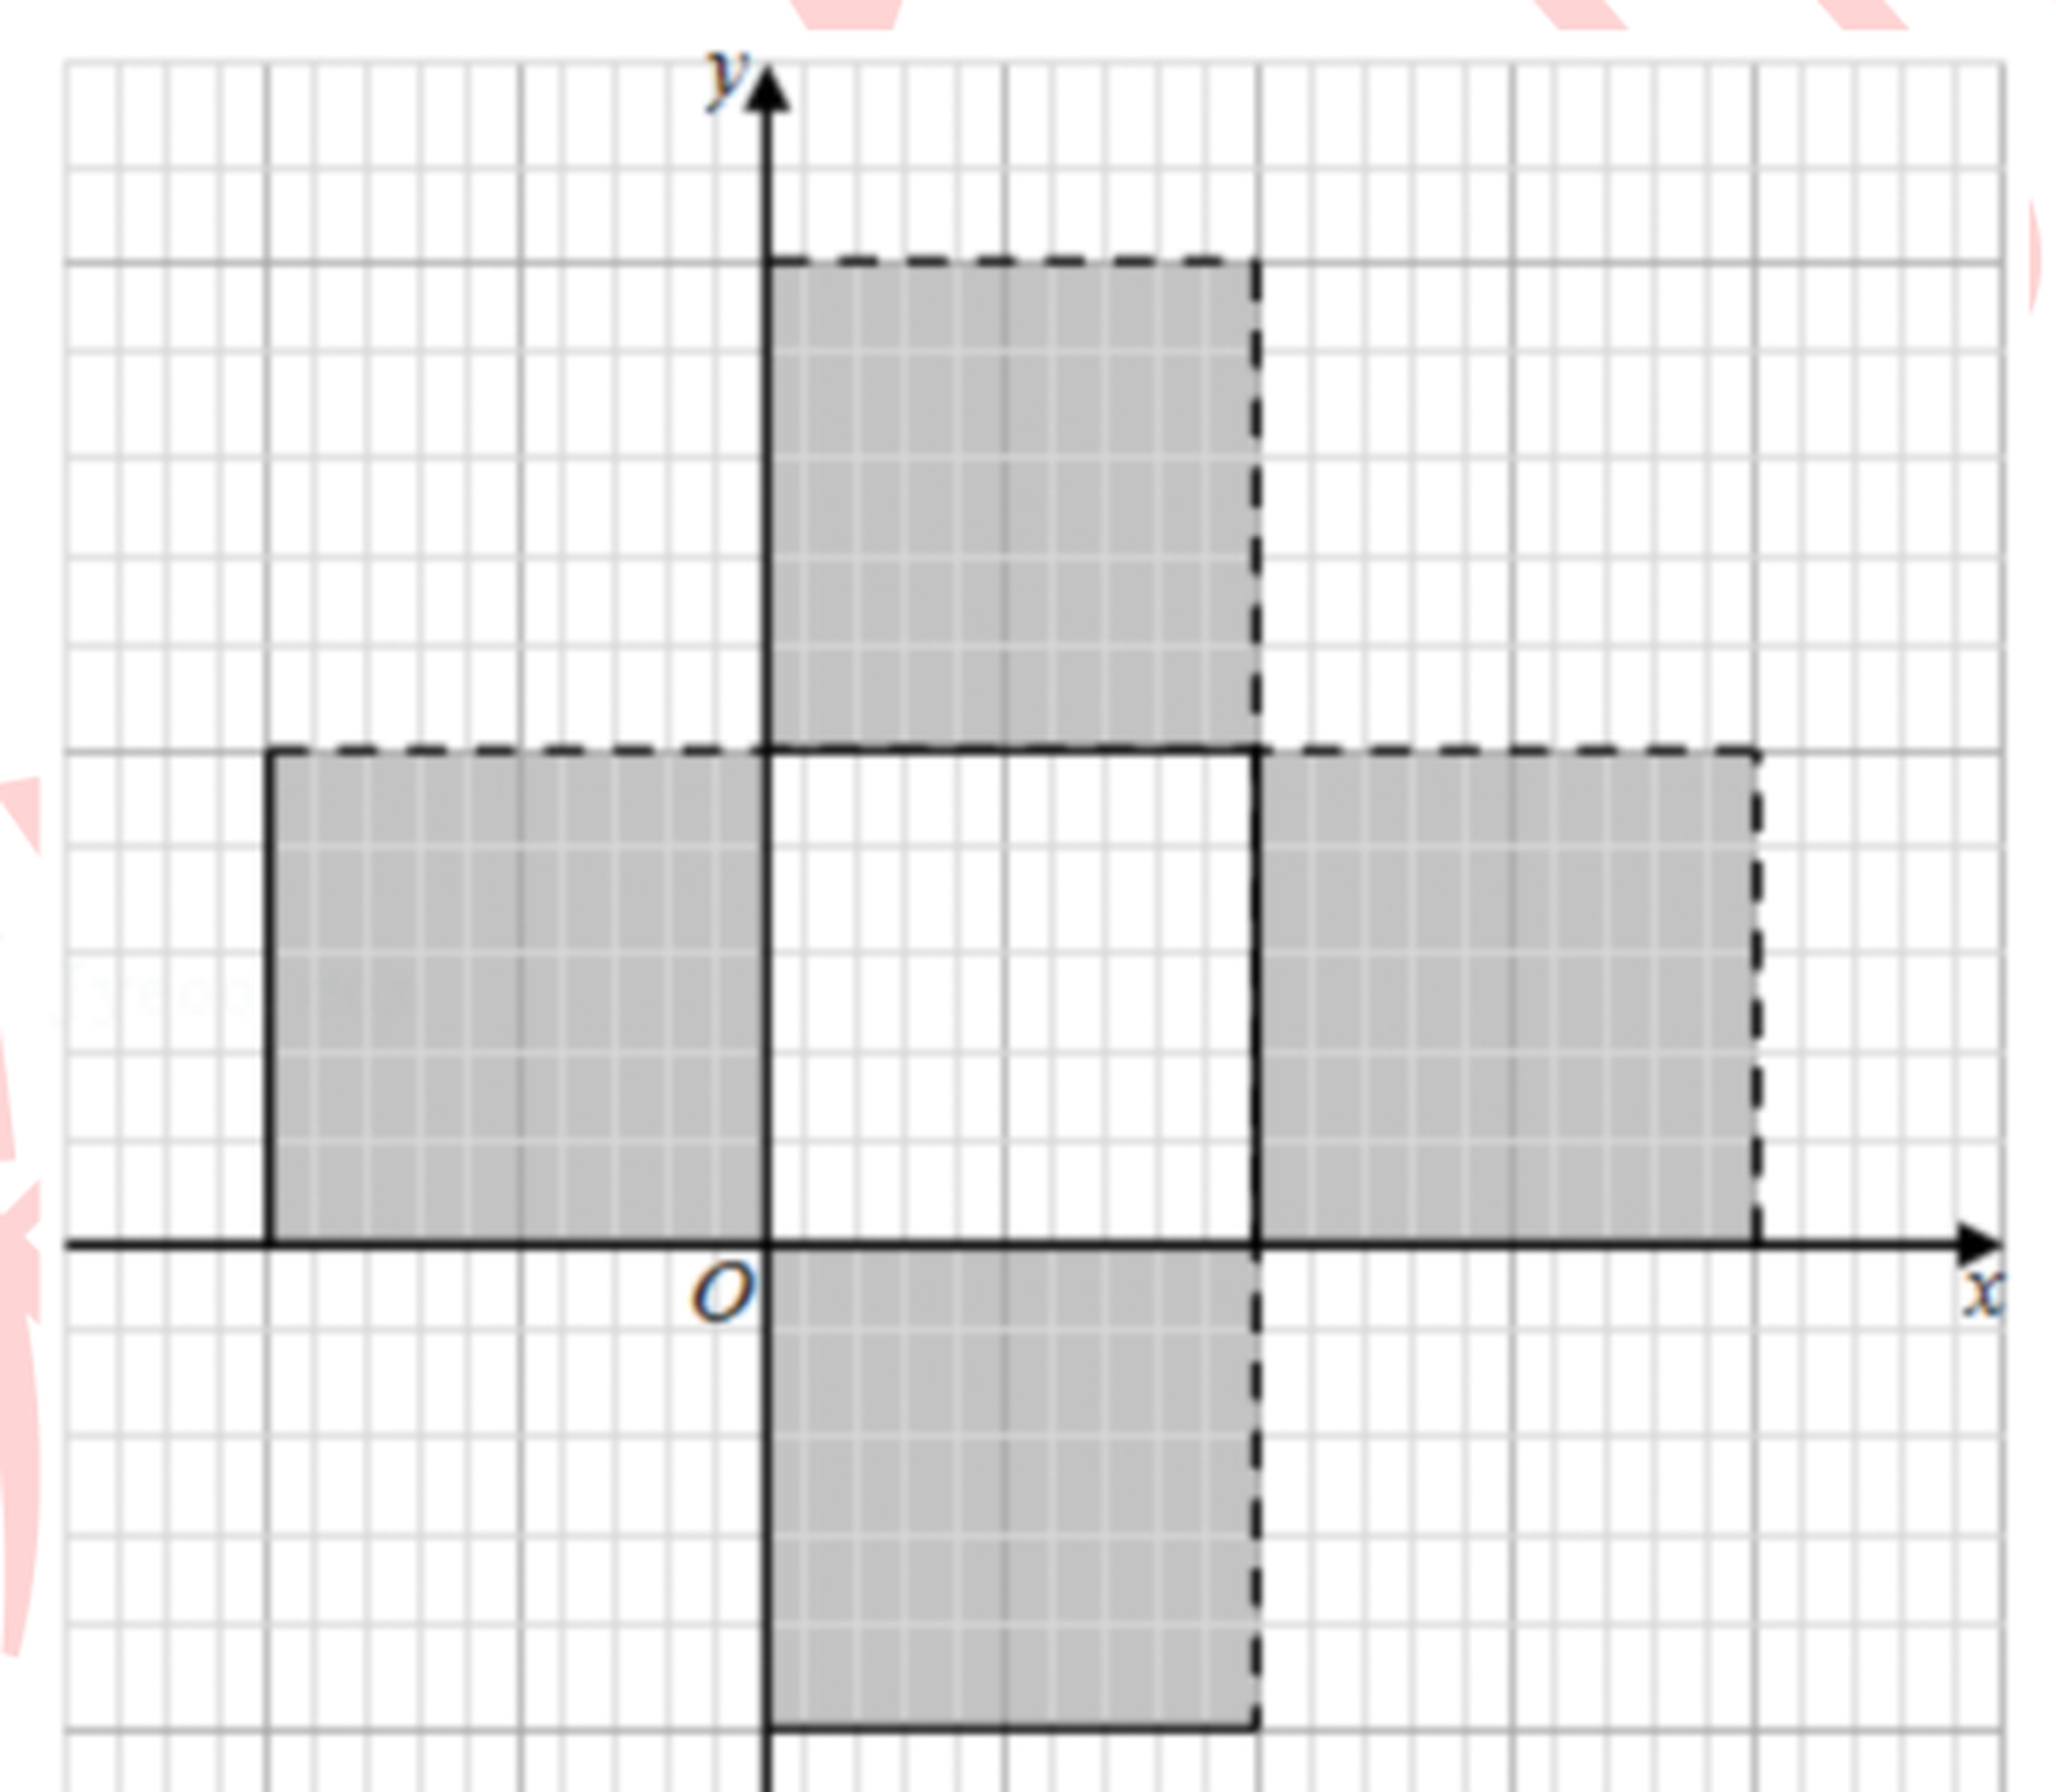
\includegraphics[width=0.38\textwidth]{figures/plane_grid_4squares_h39.png}
\end{center}
\step{总面积为 $1\times4=4$.}
\solend

\fi

\item 关于 $x$ 的不等式 $ax^2+bx+c>0$ 的解集为 $\{x\mid x<\beta\text{ 或 }x>\gamma\}(0<\beta<\gamma)$，
则不等式 $a(x^2+1)+b(x-1)+c>2ax$ 的解集为 \blankline[4.4em].

\ans{$(-\infty,\beta+1)\cup(\gamma+1,+\infty)$}

\ifanswer
\solbegin
\step{由题意得 $\beta$、$\gamma$ 为方程 $ax^2+bx+c=0$ 的两根且 $a>0$，}
\step{则 $\beta+\gamma=-\dfrac ba$，$\beta\gamma=\dfrac ca$，故 $b=-a(\beta+\gamma)$，$c=\beta\gamma a$，}
\step{则不等式可化为 $a(x^2+1)-a(\beta+\gamma)(x-1)+\beta\gamma a>2ax$，}
\step{因为 $a>0$，所以 $x^2+1-(\beta+\gamma)(x-1)+\beta\gamma>2x$，}
\step{即 $x^2-(\beta+\gamma+2)x+(\beta+\gamma+\beta\gamma+1)>0$，所以 $(x-\beta-1)(x-\gamma-1)>0$，}
\step{解得 $x<\beta+1$ 或 $x>\gamma+1$，所以不等式解集为 $(-\infty,\beta+1)\cup(\gamma+1,+\infty)$.}
\solend

\fi

\end{enumerate}

\bigsec{二、选择题}

\begin{enumerate}
\setcounter{enumi}{12}

\item 设 $a<b<0$，则下列不等式中不成立的是\mbox{（\quad）}

\keepwithprev
A. $\dfrac1a>\dfrac1b$\qquad B. $\dfrac{1}{a-b}>\dfrac1a$\qquad C. $|a|>-b$\qquad D. $\sqrt{-a}>\sqrt{-b}$

\ans{$B$}

\ifanswer
\solbegin
\step{令 $a=-2$，$b=-1$，}
\step{A、$-\dfrac12>-1$，正确；B、$-1<-\dfrac12$，故 B 错误；C、$2>1$，正确；}
\step{D、$\sqrt2>1$，正确；故选 B.}
\solend

\fi

\item 设实数集 $\R$ 为全集，集合 $P=\{x\mid f(x)=0\}$，$Q=\{x\mid g(x)=0\}$，$H=\{x\mid h(x)=0\}$，
则方程 $\dfrac{f^2(x)+g^2(x)}{h(x)}=0$ 的解集是\mbox{（\quad）}

\keepwithprev
A. $P\cap Q\cap\overline{H}$\qquad B. $P\cap Q$\qquad C. $P\cap Q\cap H$\qquad D. $P\cap Q\cup H$

\ans{$A$}

\ifanswer
\solbegin
\step{方程 $\dfrac{f^2(x)+g^2(x)}{h(x)}=0$ 等价于 $\begin{cases}f(x)=0\\ g(x)=0\\ h(x)\neq0\end{cases}$，}
\step{又因为 $P=\{x\mid f(x)=0\}$，$Q=\{x\mid g(x)=0\}$，$H=\{x\mid h(x)=0\}$，}
\step{所以方程 $\dfrac{f^2(x)+g^2(x)}{h(x)}=0$ 的解集是 $P\cap Q\cap\overline{H}$，故选 A.}
\solend

\fi

\item 设全集 $U$，在下列条件中，是 $B\sub A$ 的充要条件的有\mbox{（\quad）}

\keepwithprev
% 注：原卷此行 ② 与 ③ 之间**漏排分隔号**（①、③ 后都有「；」，② 后没有）；
%     本稿照录未补，见文件头「原卷笔误/存疑」⑩。
①$A\cup B=A$；\qquad ②$\overline{A}\cap B=\varnothing$\qquad ③$\overline{A}\sub\overline{B}$；\qquad ④$A\cup\overline{B}=U$

\keepwithprev
A. $1$ 个\qquad B. $2$ 个\qquad C. $3$ 个\qquad D. $4$ 个

\ans{$D$}

\item 已知集合 $M=\{x\mid x\in\N,0<x\leqslant15\}$，$A_1$、$A_2$、$A_3$ 满足：①$A_1\cup A_2\cup A_3=M$；
②每个集合都恰有 $5$ 个元素. 集合 $A_i(i=1,2,3)$ 中最大元素与最小元素之和称为 $A_i$ 的特征数，
记为 $X_i(i=1,2,3)$，则 $X_1+X_2+X_3$ 的值不可能为\mbox{（\quad）}

\keepwithprev
A. $37$\qquad B. $39$\qquad C. $48$\qquad D. $57$

\ans{$A$}

\ifanswer
\solbegin
\step{因为集合 $M=\{x\mid x\in\N,0<x\leqslant15\}=\{1,2,3,\cdots,15\}$，}
\step{又因为集合 $A_1$、$A_2$、$A_3$ 中，每个集合恰有 $5$ 个元素，}
\step{且 $A_1\cup A_2\cup A_3=M$ 有 $15$ 个元素，所以集合 $A_1$、$A_2$、$A_3$ 中没有重复元素，}
\step{因为 $1$ 是集合 $M$ 中数值最小的元素，$15$ 是集合 $M$ 中数值最大的元素，}
\step{所以在 $A_i$ 的特征数构成中，必有 $1$ 和 $15$，不妨设 $1\in A_1$，$15\in A_1$，}
% 注：原卷本行（与下面「最小」那句）在「集合」后的角标是**数字 $1$**（同句 $X_1$ 的角标同形），
%     而非上一行「$A_i$ 的特征数构成」里的斜体 $A_i$——原卷两种下标并存，本稿照录、不归一，
%     见文件头「原卷笔误/存疑」⑬。
\step{要使 $X_1+X_2+X_3$ 最大，则应该在集合 $A_1$ 中首先放置数值较小的元素，}
\step{即 $A_1=\{1,2,3,4,15\}$，所以 $5$ 与 $14$ 是剩下元素中数值最小或最大的元素，}
\step{同理，不妨设 $5\in A_2$，$14\in A_2$，接着在 $A_2$ 中再次放置数值较小的元素，}
\step{即 $A_2=\{5,6,7,8,14\}$，则 $A_3=\{9,10,11,12,13\}$，}
\step{此时 $X_1+X_2+X_3$ 有最大值为 $1+15+5+14+9+13=57$，}
\step{即 $X_1+X_2+X_3\leqslant57$；}
% 注：同上一处——原卷此行角标是**数字 $1$**（$A_1$），本稿照录，未与「$A_i$」归一。
\step{要使 $X_1+X_2+X_3$ 最小，则在集合 $A_1$ 中首先放置数值较大的元素，}
\step{即 $A_1=\{1,12,13,14,15\}$，所以 $2$ 与 $11$ 是剩下元素中数值最小或最大的元素，}
\step{同理，不妨设 $2\in A_2$，$11\in A_2$，接着在 $A_2$ 中再次放置数值较大的元素，}
\step{即 $A_2=\{2,8,9,10,11\}$，则 $A_3=\{3,4,5,6,7\}$，}
\step{此时 $X_1+X_2+X_3$ 有最小值为 $1+15+2+11+3+7=39$，}
\step{即 $X_1+X_2+X_3\geqslant39$，}
\step{综上，$39\leqslant X_1+X_2+X_3\leqslant57$，故选 A.}
\solend

\fi

\end{enumerate}

\bigsec{三、解答题}

\begin{enumerate}
\setcounter{enumi}{16}

% 注：原卷首句「由数 $y=-x^2+ax-1=-x+3$」中的「由数」显系「由」或「由函数」之误；末段
%     的两处分类讨论与结论自相矛盾（详见文件头「笔误/存疑」④）。本稿一律照录，未改。
\item 命题 $p$：函数 $y=-x^2+ax-1$ 与 $y=-x+3$ 图象交点的横坐标均为负值，
命题 $q$：关于 $x$ 的方程 $2(1-x)a+(x^2-10x-3)=0$ 的两个根，一个大于 $3$，另一个小于 $3$；
若命题 $p$ 和命题 $q$ 中有且仅有一个是真命题，求 $a$ 的取值范围.

\ans{$\R$}

\ifanswer
\solbegin
\step{由数 $y=-x^2+ax-1=-x+3$ 得 $x^2-(a+1)x+4=0$，}
\step{若横坐标均为负值，则满足 $\begin{cases}\Delta=(a+1)^2-16\geqslant0\\ x_1x_2=4>0\\ x_1+x_2=a+1<0\end{cases}$
得 $\begin{cases}a\geqslant3\text{ 或 }a\leqslant-5\\ a<-1\end{cases}$，得 $a\leqslant-5$，}
\step{即 $p:a\leqslant-5$，}
\step{若方程 $2(1-x)a+(x^2-10x-3)=0$ 的两个根，一个大于 $3$，另一个小于 $3$；}
\step{设 $f(x)=2(1-x)a+(x^2-10x-3)$，则 $f(3)<0$，即 $-4a-24<0$，}
\step{得 $a>-6$，即 $q:a>-6$，}
\step{因为命题 $p$ 和命题 $q$ 中有且仅有一个是真命题，}
\step{若 $p$ 真 $q$ 假，则 $\begin{cases}a\leqslant-5\\ a>-6\end{cases}$，得 $a\in\R$，}
\step{若 $p$ 假 $q$ 真，则 $\begin{cases}a>-5\\ a\leqslant-6\end{cases}$，此时 $a$ 无解，}
\step{综上，实数 $a$ 的取值范围是 $\R$.}
\solend

\fi

\ansspace[8]

\item 设全集是实数集 $\R$，$A=\left\{x\mid\dfrac{1-2x}{x-3}\geqslant0\right\}$，$B=\{x\mid x^2+a\leqslant0\}$.

\begin{enumerate}[label=(\arabic*)]

\item 当 $a=-4$ 时，求 $A\cup B$；

\item 若 $\overline{A}\cap B=B$，求实数 $a$ 的取值范围.

\end{enumerate}

\ans{（1）$\{x\mid-2\leqslant x<3\}$；（2）$\left(-\dfrac14,+\infty\right)$}

\ifanswer
\solbegin
\stepm{(1)}{$A=\left\{x\mid\dfrac{1-2x}{x-3}\geqslant0\right\}=\left\{x\mid\dfrac12\leqslant x<3\right\}$，$B=\{x\mid x^2+a\leqslant0\}$.}
\step{当 $a=-4$ 时，$B=\{x\mid-2\leqslant x\leqslant2\}$，所以 $A\cup B=\{x\mid-2\leqslant x<3\}$.}
\stepm{(2)}{$\overline{A}=\left\{x\mid x\geqslant3\text{ 或 }x<\dfrac12\right\}$，$B=\{x\mid x^2+a\leqslant0\}$.}
\step{由 $\overline{A}\cap B=B$，得 $B\sub\overline{A}$，}
\step{则当 $a>0$ 时，$B=\varnothing$，满足 $B\sub\overline{A}$，则 $a>0$ 成立，}
\step{则当 $a=0$ 时，$B=\{0\}$，满足 $B\sub\overline{A}$，则 $a=0$ 成立，}
\step{当 $a<0$ 时，$B=\{x\mid-\sqrt{-a}\leqslant x<\sqrt{-a}\}$，}
\step{得 $\sqrt{-a}<\dfrac12$，即 $-\dfrac14<a<0$，}
\step{综上，实数 $a$ 的取值范围是 $\left(-\dfrac14,+\infty\right)$.}
\solend

\fi

\ansspace[6]

\item 设集合 $A=\{x\mid ax^2+2x+1=0,a\in\R\}$.

\begin{enumerate}[label=(\arabic*)]

\item 当 $A$ 中元素个数为 $1$ 时，求：$a$ 和 $A$；

\item 当 $A$ 中元素个数至少为 $1$ 时，求：$a$ 的取值范围；

\item 求：$A$ 中各元素之和.

\end{enumerate}

\ans{（1）$a=0$ 时 $A=\left\{-\dfrac12\right\}$，$a=1$ 时 $A=\{-1\}$；（2）$(-\infty,1]$；
（3）$a=0$ 时和为 $-\dfrac12$，$a<1$ 且 $a\neq0$ 时和为 $-\dfrac2a$，$a=1$ 时和为 $-1$，$a>1$ 时 $A$ 中无元素}

\ifanswer
\solbegin
\stepm{(1)}{集合 $A=\{x\mid ax^2+2x+1=0,a\in\R\}$，$A$ 中元素个数为 $1$，}
\step{所以 $a=0$ 或 $\begin{cases}a\neq0\\ \Delta=4-4a=0\end{cases}$，解得 $a=0$，$A=\left\{-\dfrac12\right\}$ 或 $a=1$，$A=\{-1\}$.}
\stepm{(2)}{当 $A$ 中元素个数至少为 $1$ 时，$a=0$ 或 $\begin{cases}a\neq0\\ \Delta=4-4a\geqslant0\end{cases}$，解得 $a\leqslant1$，}
\step{所以 $a$ 的取值范围是 $(-\infty,1]$.}
\stepm{(3)}{当 $a=0$ 时，$A$ 中元素之和为 $-\dfrac12$；}
\step{当 $a<1$ 且 $a\neq0$ 时，$A$ 中元素之和为 $-\dfrac2a$；}
\step{当 $a=1$ 时，$A$ 中元素之和为 $-1$；}
\step{当 $a>1$ 时，$A$ 中无元素.}
\solend

\fi

\ansspace[8]

\item 设 $k$ 是正整数，集合 $A$ 至少有两个元素，且 $A\sub\N^*$. 如果对于 $A$ 中的任意两个不同的
元素 $x$、$y$，都有 $|x-y|\neq k$，则称 $A$ 具有性质 $P(k)$.

\begin{enumerate}[label=(\arabic*)]

\item 试判断集合 $B=\{1,2,3,4\}$ 和 $C=\{1,4,7,10\}$ 是否具有性质 $P(2)$？并说明理由；

\item 若集合 $A=\{a_1,a_2,\cdots,a_{12}\}\sub\{1,2,\cdots,20\}$，求证：$A$ 不可能具有性质 $P(3)$；

\item 若集合 $A\sub\{1,2,\cdots,2023\}$，且同时具有性质 $P(4)$ 和 $P(7)$，求集合 $A$ 中元素个数的
最大值.

\end{enumerate}

\ans{（1）$B$ 不具有性质 $P(2)$，$C$ 具有性质 $P(2)$；（2）见解析；（3）$920$}

\ifanswer
\solbegin
\stepm{(1)}{因为 $B=\{1,2,3,4\}$，}
\step{又 $1\in\N^*$，$2\in\N^*$，$3\in\N^*$，$4\in\N^*$，但 $|4-2|=2$，}
\step{所以集合 $B$ 不具有性质 $P(2)$，}
\step{因为 $C=\{1,4,7,10\}$，}
\step{又 $1\in\N^*$，$4\in\N^*$，$7\in\N^*$，$10\in\N^*$，}
\step{但 $|4-1|=3$，$|7-1|=6$，$|10-1|=9$，$|7-4|=3$，$|10-4|=6$，$|10-7|=3$，}
\step{所以集合 $C$ 具有性质 $P(2)$，}
\stepm{(2)}{将集合 $\{1,2,\cdots,20\}$ 中的元素分为如下 $11$ 个集合，}
% 注：原卷本行 $\{8,11\}$ 与 $\{9,12\}$ 之间的分隔号误用**句号**「.」（同行其余处皆逗号），
%     本稿照录、未改，见文件头「原卷笔误/存疑」⑪。
\step{$\{1,4\}$，$\{2,5\}$，$\{3,6\}$，$\{7,10\}$，$\{8,11\}$.$\{9,12\}$，$\{13,16\}$，$\{14,17\}$，$\{15,18\}$，}
\step{$\{19\}$，$\{20\}$，}
\step{所以从集合 $\{1,2,\cdots,20\}$ 中取 $12$ 个元素，则前 $9$ 个集合至少要选 $10$ 个元素，}
\step{所以必有 $2$ 个元素取自前 $9$ 个集合中的同一集合，即存在两个元素其差为 $3$，}
\step{所以 $A$ 不可能具有性质 $P(3)$；}
\stepm{(3)}{先说明连续 $11$ 项中集合 $A$ 中最多选取 $5$ 项，}
\step{以 $1,2,3,\cdots,11$ 为例.}
\step{构造抽屉 $\{1,8\}$，$\{2,9\}$，$\{3,10\}$，$\{4,11\}$，$\{5\}$，$\{6\}$，$\{7\}$.}
\step{①$5$、$6$、$7$ 同时选，因为具有性质 $P(4)$ 和 $P(7)$，}
\step{所以选 $5$ 则不选 $1$、$9$；选 $6$ 则不选 $2$、$10$；选 $7$ 则不选 $3$、$11$；}
% 注：原卷此步推理不严——「只剩 $4$、$8$」但两数相差 $4$、不能同选，该情形实际最多只能取 $4$ 个；
%     末句「不超过 $5$ 个」的结论仍成立。本稿照录，见文件头「原卷笔误/存疑」⑫。
\step{则只剩 $4$、$8$；故 $1,2,3,\cdots,11$ 中属于集合 $A$ 的元素个数不超过 $5$ 个.}
\step{②$5$、$6$、$7$ 选 $2$ 个，}
\step{若只选 $5$、$6$，则 $1$、$2$、$9$、$10$、$7$ 不可选，又 $\{4,11\}$ 只能选一个元素，}
\step{$3$、$8$ 可以选，故 $1,2,3,\cdots,11$ 中属于集合 $A$ 的元素个数不超过 $5$ 个.}
\step{若选 $5$、$7$，则只能从 $2$、$4$、$8$、$10$ 中选，但 $4$、$8$ 不能同时选，}
\step{故 $1,2,3,\cdots,11$ 中属于集合 $A$ 的元素个数不超过 $5$ 个.}
\step{若选 $6$、$7$，则 $2$、$3$、$10$、$11$、$5$ 不可选，又 $\{1,8\}$ 只能选一个元素，}
\step{$4$、$9$ 可以选，故 $1,2,3,\cdots,11$ 中属于集合 $A$ 的元素个数不超过 $5$ 个.}
\step{③$5$、$6$、$7$ 中只选 $1$ 个，}
\step{又四个集合 $\{1,8\}$，$\{2,9\}$，$\{3,10\}$，$\{4,11\}$ 每个集合至多选 $1$ 个元素，}
\step{故 $1,2,3,\cdots,11$ 中属于集合 $A$ 的元素个数不超过 $5$ 个.}
\step{由上述①②③得，连续 $11$ 项自然数中属于集合 $A$ 的元素至多只有 $5$ 个，}
\step{如取 $1$、$4$、$6$、$7$、$9$.}
\step{因为 $2023=183\times11+10$，则把每 $11$ 个连续自然数分组，}
\step{前 $183$ 组每组至多选取 $5$ 项；}
\step{从 $2014$ 开始，最后 $10$ 个数至多选取 $5$ 项，}
\step{故集合 $A$ 的元素最多有 $184\times5=920$ 个.}
\step{给出如下选取方法：从 $1,2,3,\cdots,11$ 中选取 $1$、$4$、$6$、$7$、$9$；}
\step{然后在这 $5$ 个数的基础上每次累加 $11$，构造 $183$ 次.}
\step{此时集合 $A$ 的元素为 $1$，$4$，$6$，$7$，$9$；$12$，$15$，$17$，$18$，$20$；$23$，$26$，$28$，$29$，$31$；
$\cdots$；$2014$，$2017$，$2019$，$2020$，$2022$，共 $920$ 个元素.}
\step{经检验得该集合符合要求，故集合 $A$ 的元素最多有 $920$ 个.}
\solend

\fi

\ansspace[10]

\end{enumerate}

\bigsec{附加题}

\begin{enumerate}
\setcounter{enumi}{20}

\item 若规定集合 $M=\{a_1,a_2,\cdots,a_n\}$（$n\in\N^*$）的子集 $\{a_{i_1},a_{i_2},\cdots,a_{i_m}\}$（$m\in\N^*$）
为 $M$ 的第 $k$ 个子集，其中 $k=2^{i_1-1}+2^{i_2-1}+\cdots+2^{i_m-1}$，则 $M$ 的第 $25$ 个子集是 \blankline[4.4em].

\ans{$\{a_1,a_4,a_5\}$}

\ifanswer
\solbegin
\step{由题意得 $M$ 的第 $k$ 个子集，且 $k=2^{i_1-1}+2^{i_2-1}+\cdots+2^{i_m-1}$，}
\step{又 $25=2^0+2^3+2^4=2^{1-1}+2^{4-1}+2^{5-1}$，所以 $M$ 的第 $25$ 个子集是 $\{a_1,a_4,a_5\}$.}
\solend

\fi

% 注：原卷在 $x=1$、$y=2$、$z=3$ 时把 $B=\{x,y\}$ 印作 $\{1,3\}$（应为 $\{1,2\}$），
%     照录未改，见文件头「笔误/存疑」⑥。
\item 用 $|S|$ 表示集合 $S$ 中的元素的个数，设 $A$、$B$、$C$ 为集合，称 $(A,B,C)$ 为有序三元组.
如果集合 $A$、$B$、$C$ 满足 $|A\cap B|=|B\cap C|=|C\cap A|=1$，且 $A\cap B\cap C=\varnothing$，
则称有序三元组 $(A,B,C)$ 为最小相交. 由集合 $\{1,2,3\}$ 的子集构成的所有有序三元组中，
最小相交的有序三元组的个数为 \blankline[4.4em].

\ans{$6$}

\ifanswer
\solbegin
\step{因为 $|A\cap B|=|B\cap C|=|C\cap A|=1$，}
\step{所以设 $A\cap B=\{x\}$，$B\cap C=\{y\}$，$C\cap A=\{z\}$，}
% 图在【解析】内（仅答案版出），取原卷截图（10.png，2560×3620）右栏，4× LANCZOS 放大。
\begin{center}
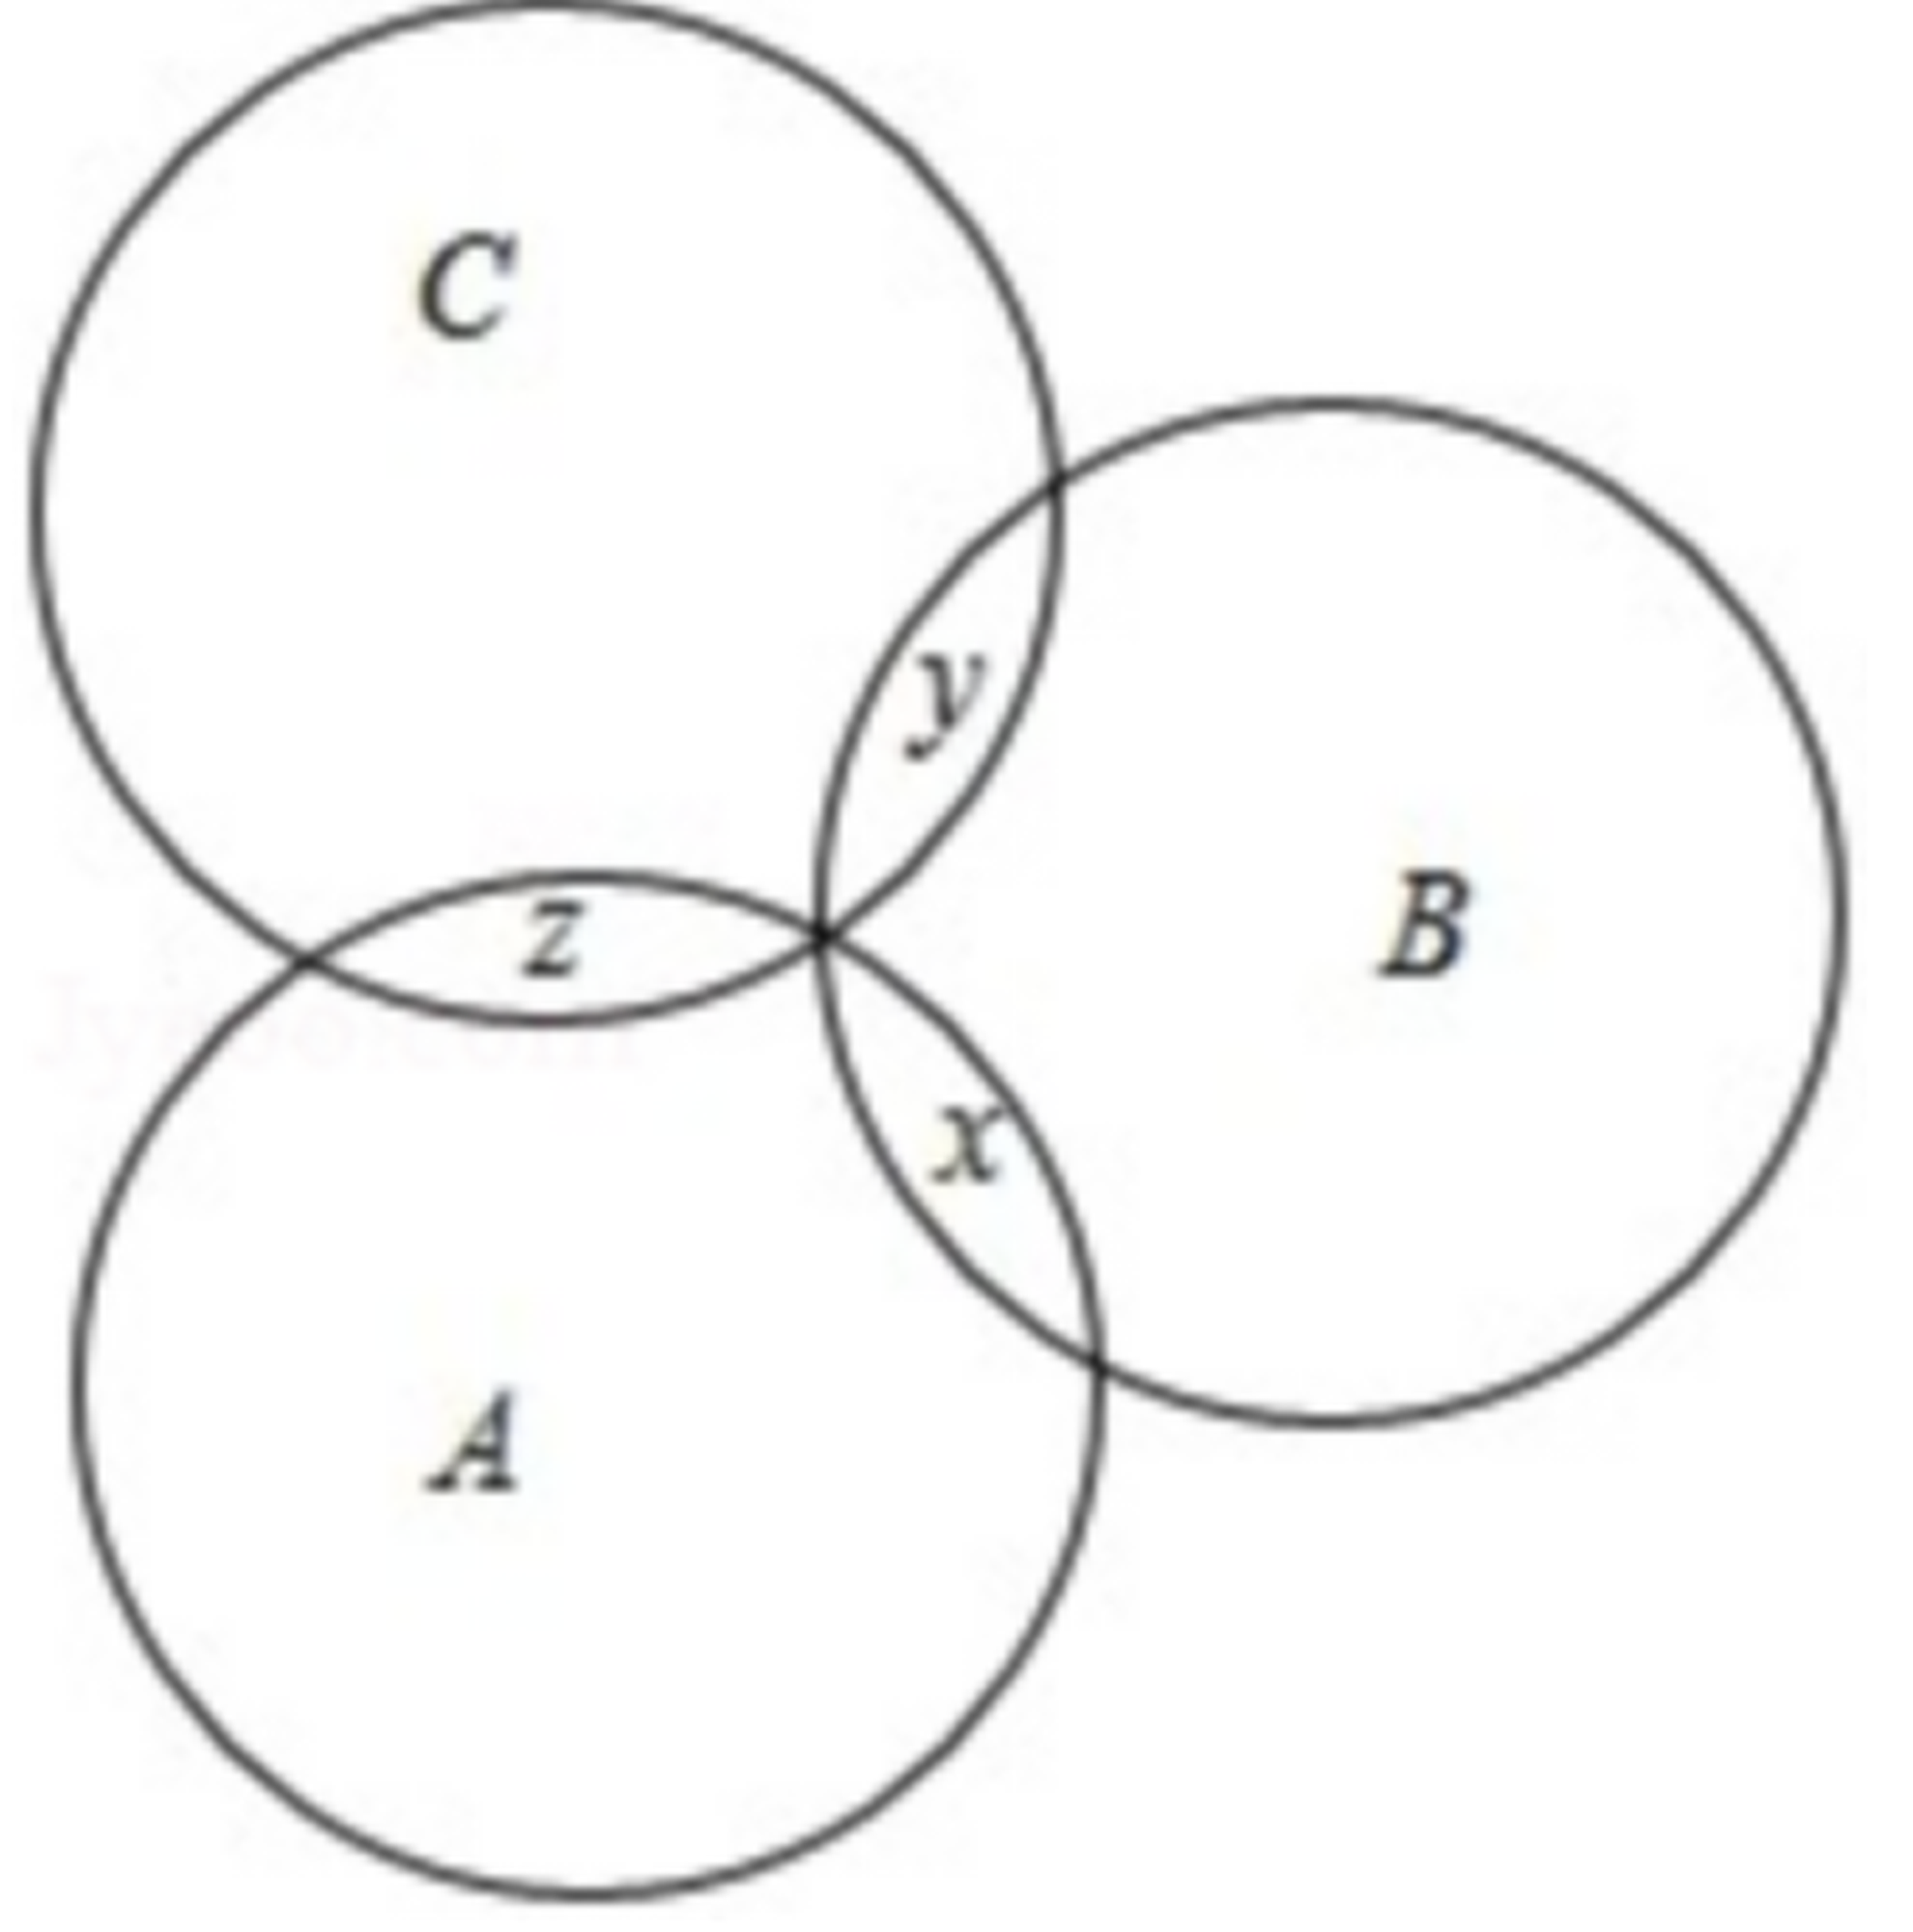
\includegraphics[width=0.30\textwidth]{figures/venn_ABC_x_y_z_h39.png}
\end{center}
\step{因为 $|A\cap B|=|B\cap C|=|C\cap A|=1$，且 $x$、$y$、$z\in\{1,2,3\}$，}
\step{所以集合 $A=\{x,z\}$，$B=\{x,y\}$，$C=\{z,y\}$，}
\step{若 $x=1$，$y=2$，$z=3$，则 $A=\{1,3\}$，$B=\{1,3\}$，$C=\{2,3\}$，}
\step{将 $1$，$2$，$3$ 进行全排列，有 $P_3^3=3\times2=6$ 个.}
\solend

\fi

\item 已知集合 $T=\{1,2,\cdots,2025\}$，对于 $T$ 的每一个非空子集的所有元素，计算它们乘积的倒数，
则所有这样倒数的和为 \blankline[4.4em].

\ans{$2025$}

\ifanswer
\solbegin
\step{集合 $T=\{1,2,\cdots,2025\}$ 的非空子集的个数为 $2^{2025}-1$，}
\step{这些子集中，每个元素的乘积分别为}
\step{$1,2,3,\cdots,2025,1\times2,1\times3,\cdots,1\times2025,\cdots,1\times2\times3\times\cdots\times2025$，}
\step{每项都可以看作是从 $1,2,3,\cdots,2025$ 中选择若干项的乘积，}
\step{$1+\dfrac12+\cdots+\dfrac{1}{2025}+\dfrac{1}{1\times2}+\dfrac{1}{1\times3}+\cdots+\dfrac{1}{2024\times2025}
+\cdots+\dfrac{1}{1\times2\times\cdots\times2025}$}
\step{$=(1+1)\left(1+\dfrac12\right)\cdots\left(1+\dfrac{1}{2025}\right)-1
=2\times\dfrac32\times\dfrac43\times\cdots\times\dfrac{2026}{2025}-1=2025$.}
\solend

\fi

% 第 24 题是压轴题，题干较长；试卷版在它之前量一次页高，尽量不与前文分家（照全稿成例）。
\ansneed{5cm}
% 注：原卷【解析】①③ 两步把 $f(x)$ 印作 $f[x[x]]$，显系笔误，照录未改，见文件头「笔误/存疑」⑦。
\item 若 $X$ 是一个集合，$T$ 是一个以 $X$ 的某些子集为元素的集合，且满足：①$X$ 属于 $T$，
$\varnothing$ 属于 $T$；②$T$ 中任意多个元素的并集属于 $T$；③$T$ 中任意多个元素的交集属于 $T$.
则称 $T$ 是集合 $X$ 上的一个拓扑. 已知函数 $f(x)=[x[x]]$，其中 $[x]$ 表示不大于 $x$ 的最大整数，
当 $x\in(0,n]$，$n\in\N^*$ 时，函数 $f(x)$ 值域为集合 $A_n$，则集合 $A_2$ 上的含有 $4$ 个元素的
拓扑 $T$ 的个数为 \blankline[4.4em].

\ans{$9$}

\ifanswer
\solbegin
\step{由题意，$n=2$，故 $0<x\leqslant2$，}
\step{①当 $0<x<1$ 时，则 $[x]=0$，所以 $f[x[x]]=0$，}
\step{②当 $x=1$ 时，$[x]=1$ 显然 $f(1)=1$，}
\step{③当 $1<x<2$ 时，$[x]=1$，所以 $f[x[x]]=[x]=1$，}
\step{④当 $x=2$ 时，$f(2)=4$，}
\step{所以 $A_2=\{0,1,4\}$，}
\step{因为 $T$ 中含有 $4$ 个元素，其中两个元素 $\varnothing$ 和 $A_2$，}
\step{$A_2=\{0,1,4\}$. 其它两个元素为 $A$、$B$，则
$\begin{cases}A\neq\varnothing\\ A\neq A_2\\ B\neq\varnothing\\ B\neq A_2\\ A\neq B\end{cases}$，}
\step{由对称性，不妨设 $1\leqslant|A|\leqslant|B|\leqslant2$，其中 $|A|$、$|B|$ 表示集合 $A$ 中元素的个数，}
\step{因为 $\begin{cases}A\cap B\in T\\ A\cup B\in T\end{cases}$，又 $|A|\leqslant|B|$，所以 $A\cap B=\varnothing$ 或 $A$，}
\step{若 $A\cap B=\varnothing$，则 $A\cup B$ 只能等于 $A_2$，}
\step{（若 $A\cup B=B$，则 $A\sub B$，则 $A\cap B=A=\varnothing$，矛盾）}
\step{则必有 $\begin{cases}|A|=1\\ |B|=2\end{cases}$，所以 $(A,B)$ 的个数 $\Leftrightarrow$ $A$ 的个数 $=3$ 种，}
\step{即 $\begin{cases}A=\{0\}\\ B=\{1,4\}\end{cases}$ 或 $\begin{cases}A=\{1\}\\ B=\{0,4\}\end{cases}$
或 $\begin{cases}A=\{4\}\\ B=\{0,1\}\end{cases}$；}
\step{若 $A\cap B=A\Leftrightarrow A\sub B$ 此时满足 $A\cup B=B$，}
\step{因为 $A\neq B$ 且 $1\leqslant|A|$ 且 $|B|\leqslant2$，所以 $\begin{cases}|A|=1\\ |B|=2\end{cases}$，}
\step{所以 $B$ 的选择共有 $C_3^2=3$ 种，则 $A$ 的个数有 $C_2^1$ 种，}
\step{所以 $(A,B)$ 的个数 $=2\times3=6$ 种.}
% 这六组「$A$／$B$」按原卷排作两行（前五个一行、第六个另起一行）；因五组并排时
% amsmath 的 cases 会为每组的第二列各留一枚 \quad，本行改排 \left\{\begin{matrix}…\end{matrix}\right.
% 以省下这枚 \quad（照 README「说明」记的高一07 成例），字形与 cases 相同。
\step{（这 $6$ 种是 $\left\{\begin{matrix}A=\{0\}\\ B=\{0,1\}\end{matrix}\right.$、
$\left\{\begin{matrix}A=\{1\}\\ B=\{0,1\}\end{matrix}\right.$、
$\left\{\begin{matrix}A=\{0\}\\ B=\{0,4\}\end{matrix}\right.$、
$\left\{\begin{matrix}A=\{4\}\\ B=\{0,4\}\end{matrix}\right.$、
$\left\{\begin{matrix}A=\{1\}\\ B=\{1,4\}\end{matrix}\right.$、}
\step{$\left\{\begin{matrix}A=\{4\}\\ B=\{1,4\}\end{matrix}\right.$）.}
\step{综上，$T$ 的个数为 $9$ 个.}
\solend

\fi

\end{enumerate}

\end{document}
"
%
% 原始材料是微信公众号图文（公众号「魔都数学加油站」连载「27学年高一 39」，署名「破晓」，
% 2026-09-26 21:29 发布，原文标题「27学年高一39——2026-2027年上海市大同中学高一上周末作业4.1」，
% 原文链接 https://mp.weixin.qq.com/s/HR2hIayXUXNi4zTs3PioiQ ），正文为 11 张 PNG 页。**同一篇里各页分辨率不一致**（2560×3620 与 4762×6735 两档混排：第 1、3、8、10 页为
% 2560×3620，第 2、4、5、6、7、9、11 页为 4762×6735）。原文本身就是一份**讲评版**——除第 15 题
% 外各题题下直接印【解析】（无单独的【答案】行），第 15 题的答案「D」直接印在题干末尾的括号内。
% 试题文字、答案与解析均照原卷录入，未改内容。卷面的粉色斜水印「魔都数学加油站」属水印，未录入。
%
% 卷首标题：原卷页首印作「2026-2027 年大同中学高一上周末作业 4.1」（**卷面标题行即带校名**，
% 年份区间按全稿惯例排 en dash，前缀照原卷保留「年」）。
%
% 篇幅与题号：卷面自「一、填空题」的**第 3 题**起编，终于「附加题」的**第 24 题**，共 22 题
% （填空 3—12、选择 13—16、解答 17—20、附加题 21—24）。第 1、2 题未在该文中发布——这是该
% 公众号连载讲评版的通例（高一02—高一09 等均自第 3 题起编，README「说明」已记），**不是截断**，
% 故本稿题号亦自 3 起。它与 高一40（大同中学 周末作业4.2）同属「周末作业 4」系列但**各自独立起编**
% （4.2 自第 3 题起、终于第 19 题），不是同一份试卷的两半。
%
% 与原卷的排版差异（均已在 README「说明」中交代）：
%   ① 原文自**第 3 题**起（第 1、2 题未在该文中发布），故本稿题号亦自 3 起，填空题以
%      \setcounter{enumi}{2} 起编；选择、解答、附加题三节各按上一节末号另设 \setcounter
%      （选择题 \setcounter{enumi}{12}、解答题 \setcounter{enumi}{16}、附加题 \setcounter{enumi}{20}）；
%   ② 原卷本就印有「一、填空题」「二、选择题」「三、解答题」三节标题，末节印作「附加题」
%      （**不带「四、」**，且题号 21—24 续前编、不另起），本稿照原卷分节，只把标题改排成全稿
%      统一的「大节标题」样式；
%   ③ 原卷是「讲评版」：除第 15 题外，各题题下均印【解析】（**全卷无一条独立的【答案】行**）；
%      第 15 题无解析，答案「D」直接印在题干末尾的括号内。本稿统一改为试卷版隐去、答案版以
%      \ans{}／\ifanswer 块给出，两版彻底分离；原卷写在【解析】末句的结果，本稿照 高一38
%      （同校同系列、同为讲评版）的成例另提为 \ans{}；
%   ④ 数集记号原卷两套并用：实数集作斜体的 $R$（第 7、11、14、17、18、19 题），整数集作斜体
%      $Z$（第 10 题），自然数集作斜体 $N$ 及 $N^*$（第 16、20、21、24 题），本稿按全稿惯例
%      统一写作 $\R$、$\Z$、$\N$、$\N^*$；
%   ⑤ 补集符号原卷两套并用：第 7 题作前缀式的 $C_U$（且题干称全集为 $I$，见「笔误/存疑」①），
%      第 14、15、18 题作上横线（$\overline{H}$、$\overline{A}$、$\overline{B}$），本稿照录、不归一
%      （前缀式写作 $\complement_U$，与 高一c／高一10 的成例一致）；
%   ⑥ 包含符号原卷两套并用：第 3 题作**无下划线**的 $\subset$，第 15、18、20、24 题作**带下划线**
%      的 $\sub$，本稿照录、不归一；
%   ⑦ 原卷填空的横线约两个字宽，本稿按全稿惯例统一排 \blankline[4.4em]；
%   ⑧ 第 7、11、22 题各有插图，取原卷截图、4× LANCZOS 放大（figures/venn_N_cap_CI_M_h39.png、
%      figures/plane_grid_4squares_h39.png、figures/venn_ABC_x_y_z_h39.png）；第 7 题的 Venn 属
%      **题干**（试卷版、答案版都出），第 11、22 题的图在【解析】内（仅答案版出）。第 7 题图
%      左下、第 11 题图的上／左／右边缘带进极淡的原卷粉色水印残影——照全稿「插图直接取自
%      原卷截图、不用 TikZ 重绘、不修图」的体例保留（再裁会切到坐标轴与 $x$、$y$、$O$ 标注）；
%   ⑨ 原卷并列的字母、数字（「$x_1,x_2$」「$a,b$」「$1,2,3,\cdots,11$」）多作半角逗号或不加标点，
%      本稿按全稿惯例改排顿号（$x_1$、$x_2$）或把数列并入行内公式；半角括号、逗号一律排全角，
%      数学式内部的标点照原样；
%   ⑩ 原卷未印副标题，本稿按**本卷实际内容**补出副标题「集合与常用逻辑用语」（依据见下条）。
%
% 副标题（\examtitlest 第二个参数）：本卷卷面未印副标题，由本稿补出，取值按 2026-09-26 起的
%   新口径「只用本卷实际内容的模块名」定为「集合与常用逻辑用语」。依据：全卷 22 题（第 3—24 题）中，
%   第 3、5、7、8、10、11、14、15、16、17、18、19、20、21、22、23、24 题共 17 题是集合的运算与
%   关系、子集／真子集、补集、集合新定义（「全食／偏食」、最小相交、拓扑、特征数）与集合计数，
%   以及命题与常用逻辑用语（第 3 题充要条件、第 5 题存在量词命题、第 17 题命题真假）；其余两题
%   第 4、6 考一元二次方程的根（韦达定理）与方程恒等，第 9、12、13 题是不等式（一元二次不等式组
%   的整数解、一元二次不等式解集、不等式的性质）——不等式合计 3/22，**不足全卷三分之一**，
%   故不并标「不等式」。
%
% 原卷笔误/存疑（均照抄原卷、未改，见源码中该处上方注释）：
%   ① 第 7 题题干称「全集 $I=R$」，而【解析】两处把补集写作 $C_U M$（下标作 $U$），前后记号不一；
%      本稿照录，未改；
%   ② 第 4 题【解析】两处把判别式印作 $\triangle=[2(m-1)^2-16m^2]$（方括号内首项漏了平方，
%      正确应作 $[2(m-1)]^2-16m^2$）；按其所判「$m=\frac12$ 时 $<0$、$m=-\frac12$ 时 $>0$」反推，
%      $[2(m-1)]^2-16m^2$ 在 $m=\frac12$ 时为 $-3<0$、在 $m=-\frac12$ 时为 $5>0$，与结论一致；
%      本稿照录；
%   ③ 第 9 题【解析】把方程组第二式印作 $1-2<-k\leqslant3$，按其结论 $-3\leqslant k<2$ 反推，
%      疑当作 $-2<-k\leqslant3$（原卷多一个「$1$」）；本稿照录；
%   ④ 第 17 题【解析】首句「由数 $y=-x^2+ax-1=-x+3$」中的「由数」显系「由」或「由函数」之误；
%      且末段「若 $p$ 真 $q$ 假…得 $a\in R$」「若 $p$ 假 $q$ 真…此时 $a$ 无解」与结论「$a$ 的取值范围
%      是 $R$」自相矛盾（按 $p:a\leqslant-5$、$q:a>-6$，$p$ 真 $q$ 假应为 $a\leqslant-6$，$p$ 假 $q$ 真
%      应为 $a>-5$，合起来是 $a\leqslant-6$ 或 $a>-5$，并非 $R$）；本稿一律照录，未按正确解法改写；
%   ⑤ 第 18 题【解析】(2) 把 $B=\{x\mid x^2+a\leqslant0\}$（$a<0$）印作右端开的
%      $\{x\mid-\sqrt{-a}\leqslant x<\sqrt{-a}\}$（应为闭的「$\leqslant$」）；按其所判
%      $\sqrt{-a}<\frac12$ 反推，不影响结论；本稿照录；
%   ⑥ 第 22 题【解析】在 $x=1$、$y=2$、$z=3$ 时把 $B=\{x,y\}$ 印作 $\{1,3\}$（应为 $\{1,2\}$），
%      与本行前面「$B=\{x,y\}$」不合；本稿照录；
%   ⑦ 第 24 题【解析】①③ 两步把 $f(x)$ 印作 $f[x[x]]$，显系笔误；本稿照录。
%   ⑧ 第 8 题【解析】「即方程 $x^2+ax+b=x$，$x^2+(a-1)x+b=0$ **由**两个相等的实数根为 $4$」——
%      「由」当为「有」（「设…是…有」的杂糅）；本稿照录；
%   ⑨ 第 10 题：题设 $a\oplus b=b(a^2+b^2+1)$，而集合定义里含 $\dfrac{a\oplus b}{2b}$；$-2<a<b<2$、
%      $a$、$b\in\Z$ 时 $(a,b)=(-1,0)$ 也合条件、却使分母 $2b=0$，原卷解析仍代入该组并约去
%      $b$ 得 $x=1$（答案集恰好不变）；本稿照录；
%   ⑩ 第 15 题选项列里 ② 与 ③ 之间**漏排分隔号**（原卷作「② $\overline{A}\cap B=\varnothing$③
%      $\overline{A}\sub\overline{B}$；」——①、③ 后都有「；」，② 后没有）；本稿照录；
%   ⑪ 第 20(2) 把 $\{1,2,\cdots,20\}$ 分成的 11 个集合里，$\{8,11\}$ 与 $\{9,12\}$ 之间误用
%      **句号**「.」（同行其余处皆逗号）；本稿照录；
%   ⑫ 第 20(3)① 推理不严：原卷写「选 5 则不选 1、9；选 6 则不选 2、10；选 7 则不选 3、11；
%      则只剩 4、8」——但 4 与 8 相差 $4$、不能同选，该情形实际最多只能取 $4$ 个；末句结论
%      「不超过 $5$ 个」仍成立；本稿照录；
%   ⑬ 第 16 题【解析】两种下标并存：「所以在 $A_i$ 的特征数构成中」原卷作斜体 $A_i$，而
%      「要使 $X_1+X_2+X_3$ 最大（小），则（应）在集合 $A_1$ 中首先放置…」两处原卷作
%      **数字 $1$**（与同句 $X_1$ 的角标同形）；本稿照录、未归一。
%
% 图取原卷截图（依次见各处的 \includegraphics 前的注释），4× LANCZOS 放大。
\documentclass[a4paper,11pt]{article}
\usepackage{common}

\begin{document}

\examtitlest[3]{2026--2027 年大同中学高一上周末作业 4.1}{集合与常用逻辑用语}

\bigsec{一、填空题}

\begin{enumerate}
\setcounter{enumi}{2}

\item “$x\geqslant a$”是“$0<x<2$”的必要非充分条件，则实数 $a$ 的取值范围是 \blankline[4.4em].

\ans{$(-\infty,0]$}

\ifanswer
\solbegin
\step{因为 $x\geqslant a$ 是 $0<x<2$ 的必要非充分条件，所以 $(0,2)\subset[a,+\infty)$，所以 $a\leqslant0$，}
\step{则实数 $a$ 的取值范围是 $(-\infty,0]$.}
\solend

\fi

% 注：原卷$[2(m-1)^2-16m^2]$ 首项漏了平方（应为 $[2(m-1)]^2-16m^2$），照录未改，见文件头「笔误/存疑」②。
\item 若关于 $x$ 的方程 $x^2+2(m-1)x+4m^2=0$ 有两个实数根，且这两根互为倒数，则 $m=$ \blankline[4.4em].

\ans{$-\dfrac12$}

\ifanswer
\solbegin
\step{设 $x_1$、$x_2$ 是方程 $x^2+2(m-1)x+4m^2=0$ 有两个实数根，}
\step{则 $x_1x_2=4m^2=1$，解得 $m=\dfrac12$ 或 $m=-\dfrac12$，}
\step{又当 $m=\dfrac12$ 时，$\triangle=[2(m-1)^2-16m^2]<0$，舍去，}
\step{当 $m=-\dfrac12$ 时，$\triangle=[2(m-1)^2-16m^2]>0$，故 $m=-\dfrac12$.}
\solend

\fi

\item 已知命题：“存在 $x\in[1,2]$，使 $x^2+2x+a\geqslant0$”为真命题，则 $a$ 的取值范围是 \blankline[4.4em].

\ans{$a\geqslant-8$}

\ifanswer
\solbegin
\step{若存在 $x\in[1,2]$，使 $x^2+2x+a\geqslant0$，}
\step{则等价为存在 $x\in[1,2]$，使 $x^2+2x\geqslant-a$，}
\step{当存在 $x\in[1,2]$ 时，设 $y=x^2+2x=(x+1)^2-1$，则 $3\leqslant y\leqslant8$，}
\step{所以要使 $x^2+2x\geqslant-a$，则 $8\geqslant-a$，即 $a\geqslant-8$.}
\solend

\fi

\item 已知方程 $a(3x+2)+b(2x-3)=8x+3$ 有无穷多个解，则 $a:b=$ \blankline[4.4em].

\ans{$30:7$}

\ifanswer
\solbegin
\step{$a(3x+2)+b(2x-3)=(3a+2b)x+2a-3b=8x+3$ 有无穷多个解，}
\step{所以 $\begin{cases}3a+2b=8\\ 2a-3b=3\end{cases}$，解得 $a=\dfrac{30}{13}$，$b=\dfrac{7}{13}$，所以 $a:b=30:7$.}
\solend

\fi

% 注：原卷题干称「全集 $I=R$」，而【解析】两处把补集写作 $C_U M$（下标作 $U$），前后记号不一；
%     照录未改，见文件头「笔误/存疑」①。
\item 已知集合 $M=\{x\mid y=\sqrt{3-x^2}\}$，$N=\{x\mid-3\leqslant x\leqslant1\}$，全集 $I=\R$，
则图中阴影部分表示的集合为 \blankline[4.4em].

% 图取原卷截图（01.png，2560×3620）右栏，4× LANCZOS 放大。
\begin{center}
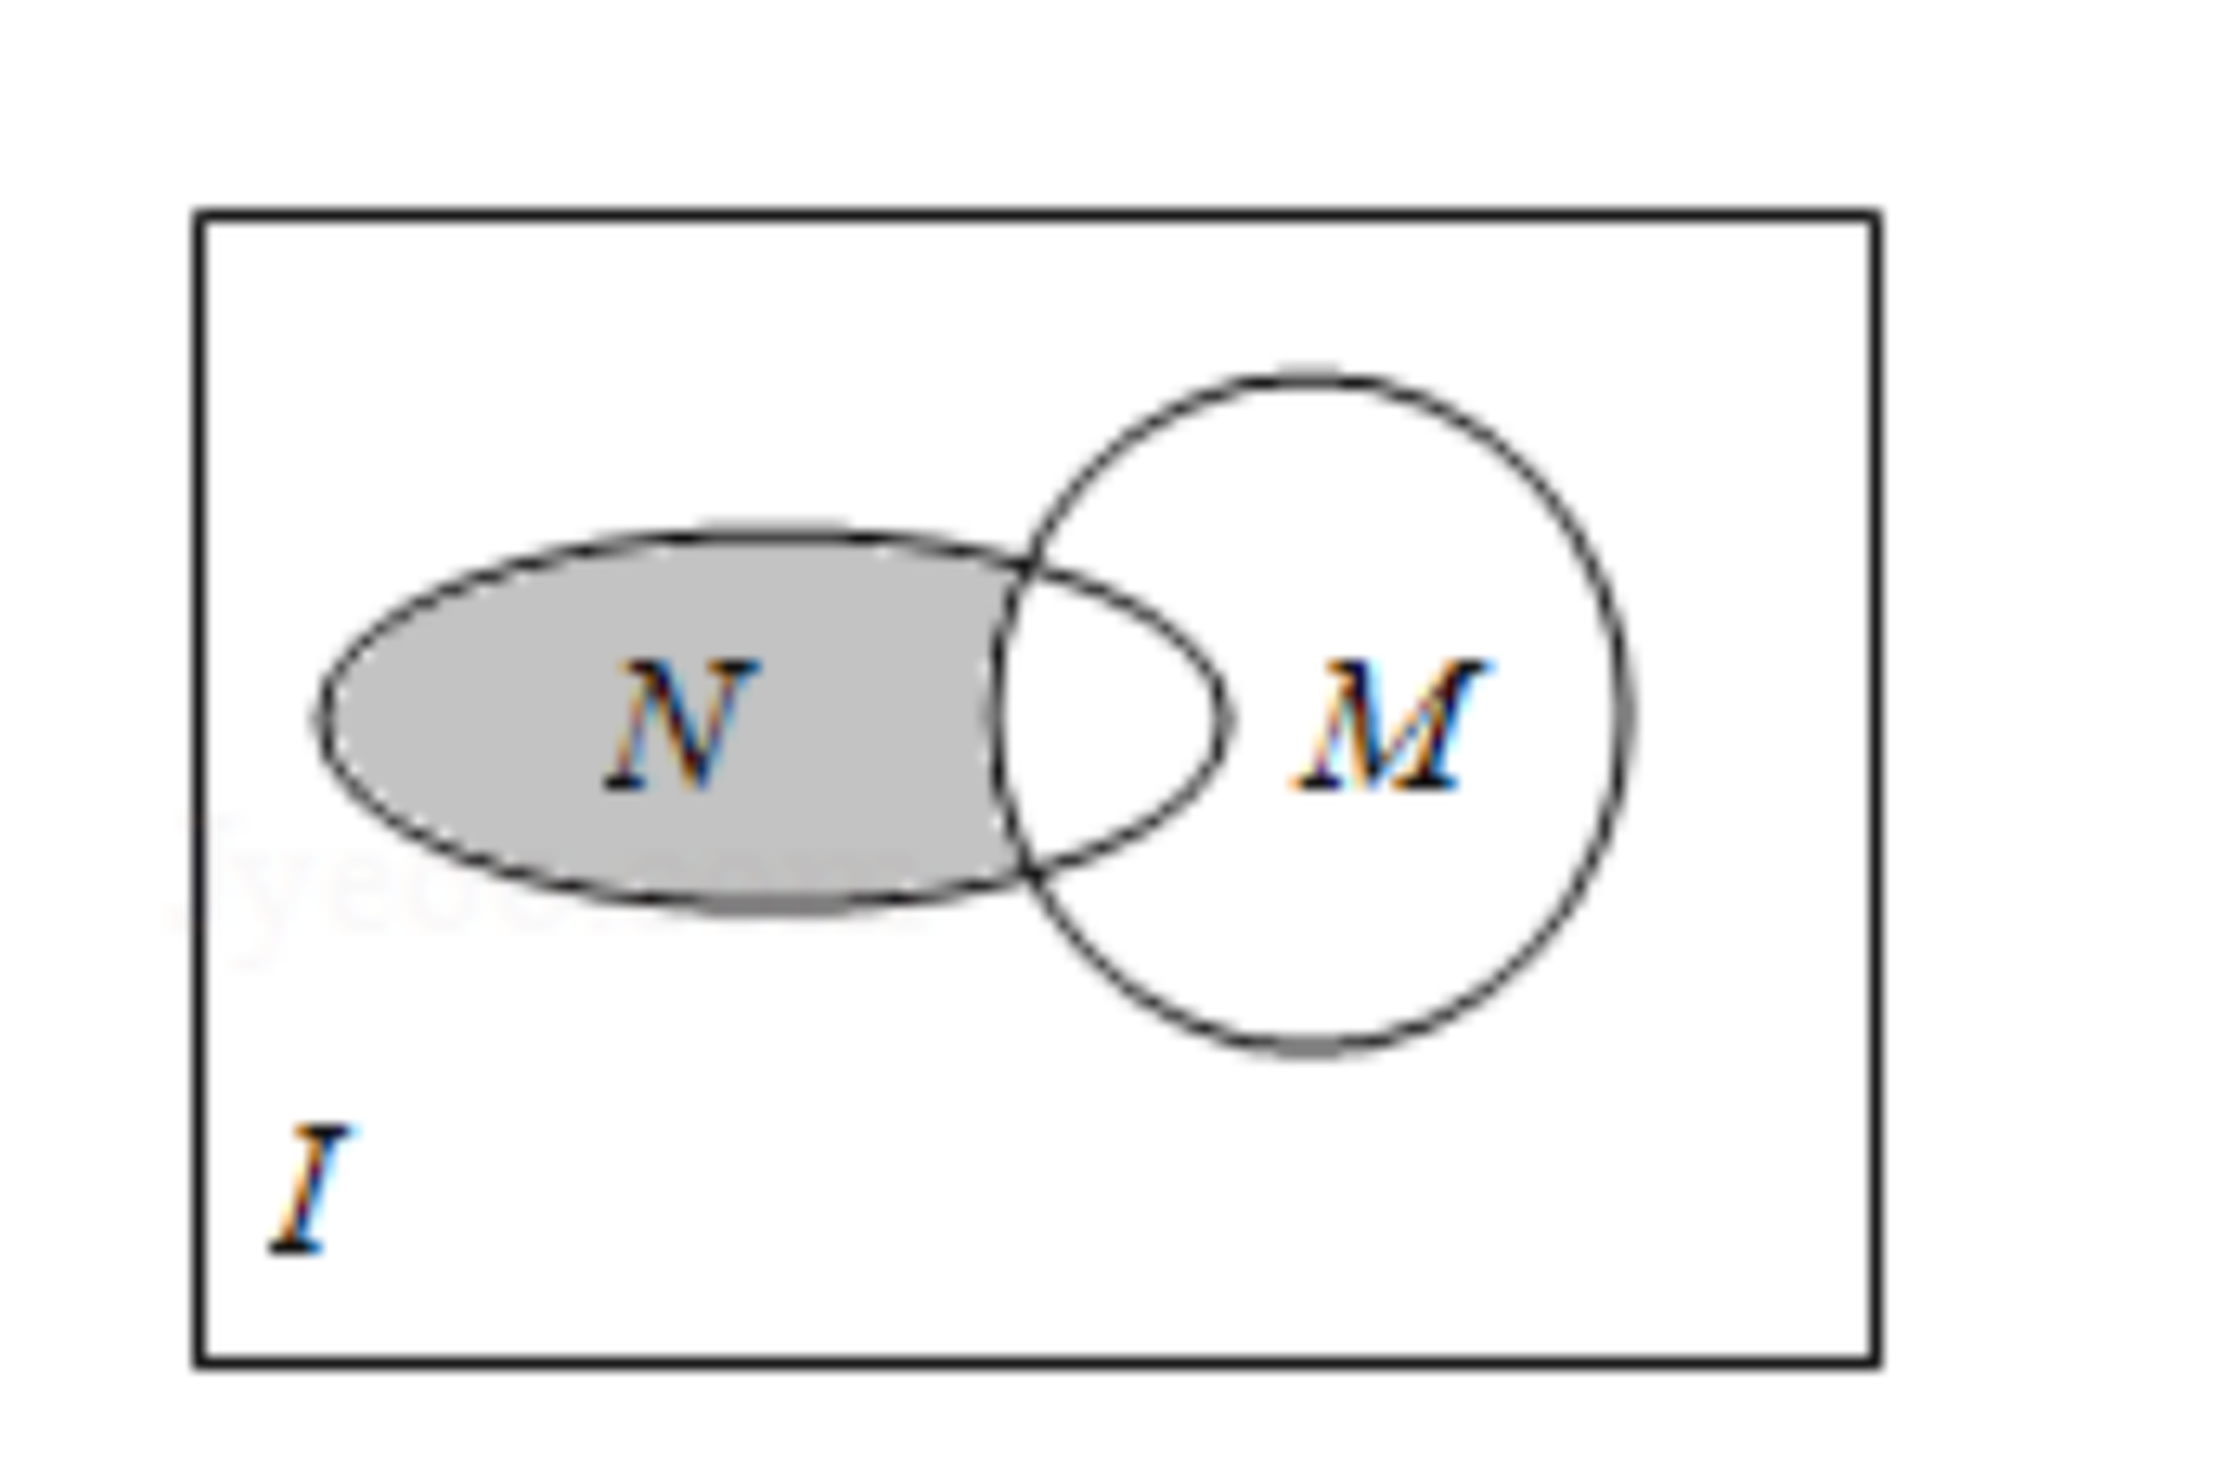
\includegraphics[width=0.30\textwidth]{figures/venn_N_cap_CI_M_h39.png}
\end{center}

\ans{$[-3,-\sqrt3)$}

\ifanswer
\solbegin
\step{阴影部分用集合表示为 $N\cap(\complement_UM)$.}
\step{则 $M=\{x\mid y=\sqrt{3-x^2}\}=\{x\mid3-x^2\geqslant0\}=\{x\mid-\sqrt3\leqslant x\leqslant\sqrt3\}$，}
\step{则 $\complement_UM=\{x\mid x>\sqrt3\text{ 或 }x<-\sqrt3\}$，$N=\{x\mid|x+1|\leqslant2\}=\{x\mid-3\leqslant x\leqslant1\}$，}
\step{则 $N\cap(\complement_UM)=\{x\mid-3\leqslant x<-\sqrt3\}$.}
\solend

\fi

\item 已知 $f(x)=x^2+ax+b$，集合 $\{x\mid f(x)=x\}=\{4\}$，将集合 $M=\{x\mid f(x)=4\}$ 用列举法表示 \blankline[4.4em].

\ans{$\{3,4\}$}

\ifanswer
\solbegin
\step{已知 $f(x)=x^2+ax+b$，集合 $\{x\mid f(x)=x\}=\{4\}$，}
% 注：原卷本行作「…$x^2+(a-1)x+b=0$ **由**两个相等的实数根为 $4$」——「由」当为「有」
%     （「设…是…有」的杂糅）；本稿照录未改，见文件头「原卷笔误/存疑」⑧。
\step{即方程 $x^2+ax+b=x$，$x^2+(a-1)x+b=0$ 由两个相等的实数根为 $4$，}
\step{所以 $\triangle=(a-1)^2-4b=0$，即 $x^2+(a-1)x+b=(x-4)^2$，所以 $b=16$，$a=-7$，}
\step{所以 $f(x)=x^2+ax+b=x^2-7x+16$，所以集合 $M=\{x\mid f(x)=4\}$，}
\step{即 $x^2-7x+16=4$，$x^2-7x+12=0$，故 $M=\{x\mid f(x)=4\}=\{3,4\}$.}
\solend

\fi

% 注：原卷方程组第二式印作 $1-2<-k\leqslant3$，按其结论 $-3\leqslant k<2$ 反推疑当作 $-2<-k\leqslant3$，
%     照录未改，见文件头「笔误/存疑」③。
\item 关于 $x$ 的不等式组 $\begin{cases}x^2-x-2>0\\ 2x^2+(2k+5)x+5k<0\end{cases}$ 的整数解的集合为 $\{-2\}$，
则实数 $k$ 的取值范围 \blankline[4.4em].

\ans{$-3\leqslant k<2$}

\ifanswer
\solbegin
\step{原不等式组即 $\begin{cases}(x-2)(x+1)>0\\ (x+k)(2x+5)<0\end{cases}$，整数解的集合为 $A$，若 $A=\{-2\}$，}
\step{则 $(-2+k)(2\times(-2)+5)<0$，所以 $k<2$，且有 $\begin{cases}-k>-\dfrac52\\ 1-2<-k\leqslant3\end{cases}$，}
\step{解得 $-3\leqslant k<2$.}
\solend

\fi

\item 规定 $\oplus$ 与 $\otimes$ 是两个运算符号，其运算法则如下，对任意实数 $a$、$b$ 有：$a\otimes b=ab$，
$a\oplus b=b(a^2+b^2+1)$. 若 $-2<a<b<2$ 且 $a$、$b\in\Z$，
$A=\left\{x\mid x=2(a\otimes b)+\dfrac{a\oplus b}{2b}\right\}$，则用列举法表示集合 $A=$ \blankline[4.4em].

\ans{$\left\{1,-\dfrac12\right\}$}

\ifanswer
\solbegin
\step{$A=\left\{x\mid x=2(a\otimes b)+\dfrac{a\oplus b}{2b}\right\}
=\left\{x\mid x=2ab+\dfrac{b(a^2+b^2+1)}{2b}\right\}$}
\step{$=\left\{x\mid x=2ab+\dfrac12a^2+\dfrac12b^2+\dfrac12\right\}
=\left\{x\mid x=\dfrac12(a+b)^2+ab+\dfrac12\right\}$，}
% 注：题设含 $\dfrac{a\oplus b}{2b}$，而 $-2<a<b<2$、$a$、$b\in\Z$ 时 $(a,b)=(-1,0)$ 也合条件、
%     却使分母 $2b=0$；原卷解析仍代入该组并约去 $b$ 得 $x=1$（答案集恰好不变）。本稿照录，
%     见文件头「原卷笔误/存疑」⑨。
\step{当 $a=-1$，$b=0$ 时，$x=1$；当 $a=-1$，$b=1$ 时，$x=-\dfrac12$；}
\step{当 $a=0$，$b=1$ 时，$x=1$；所以 $A=\left\{1,-\dfrac12\right\}$.}
\solend

\fi

\item 高斯是德国著名的数学家，近代数学奠基者之一，享有“数学王子”的称号，为了纪念数学家高斯，
我们把取整函数 $y=[x]$，$x\in\R$ 称为高斯函数，其中 $[x]$ 表示不超过 $x$ 的最大整数，
如 $[1.1]=1$，$[-1.1]=-2$. 则点集 $P=\{(x,y)\mid[x]^2+[y]^2=1\}$
所表示的平面区域的面积是 \blankline[4.4em].

\ans{$4$}

\ifanswer
\solbegin
\step{$[x]^2+[y]^2=1$ 由 $\begin{cases}[x]=0\\ [y]=-1\end{cases}$ 或 $\begin{cases}[x]=0\\ [y]=1\end{cases}$
或 $\begin{cases}[x]=-1\\ [y]=0\end{cases}$ 或 $\begin{cases}[x]=1\\ [y]=0\end{cases}$ 四个平面区域组成，}
\step{即 $\begin{cases}0\leqslant x<1\\ -1\leqslant y<0\end{cases}$ 或 $\begin{cases}0\leqslant x<1\\ 1\leqslant y<2\end{cases}$
或 $\begin{cases}-1\leqslant x<0\\ 0\leqslant y<1\end{cases}$ 或 $\begin{cases}1\leqslant x<2\\ 0\leqslant y<1\end{cases}$，}
\step{作出平面区域如图所示，平面区域由四个边长为 $1$ 的正方形组成，}
% 图在【解析】内（仅答案版出），取原卷截图（03.png，2560×3620）中部，4× LANCZOS 放大。
\begin{center}
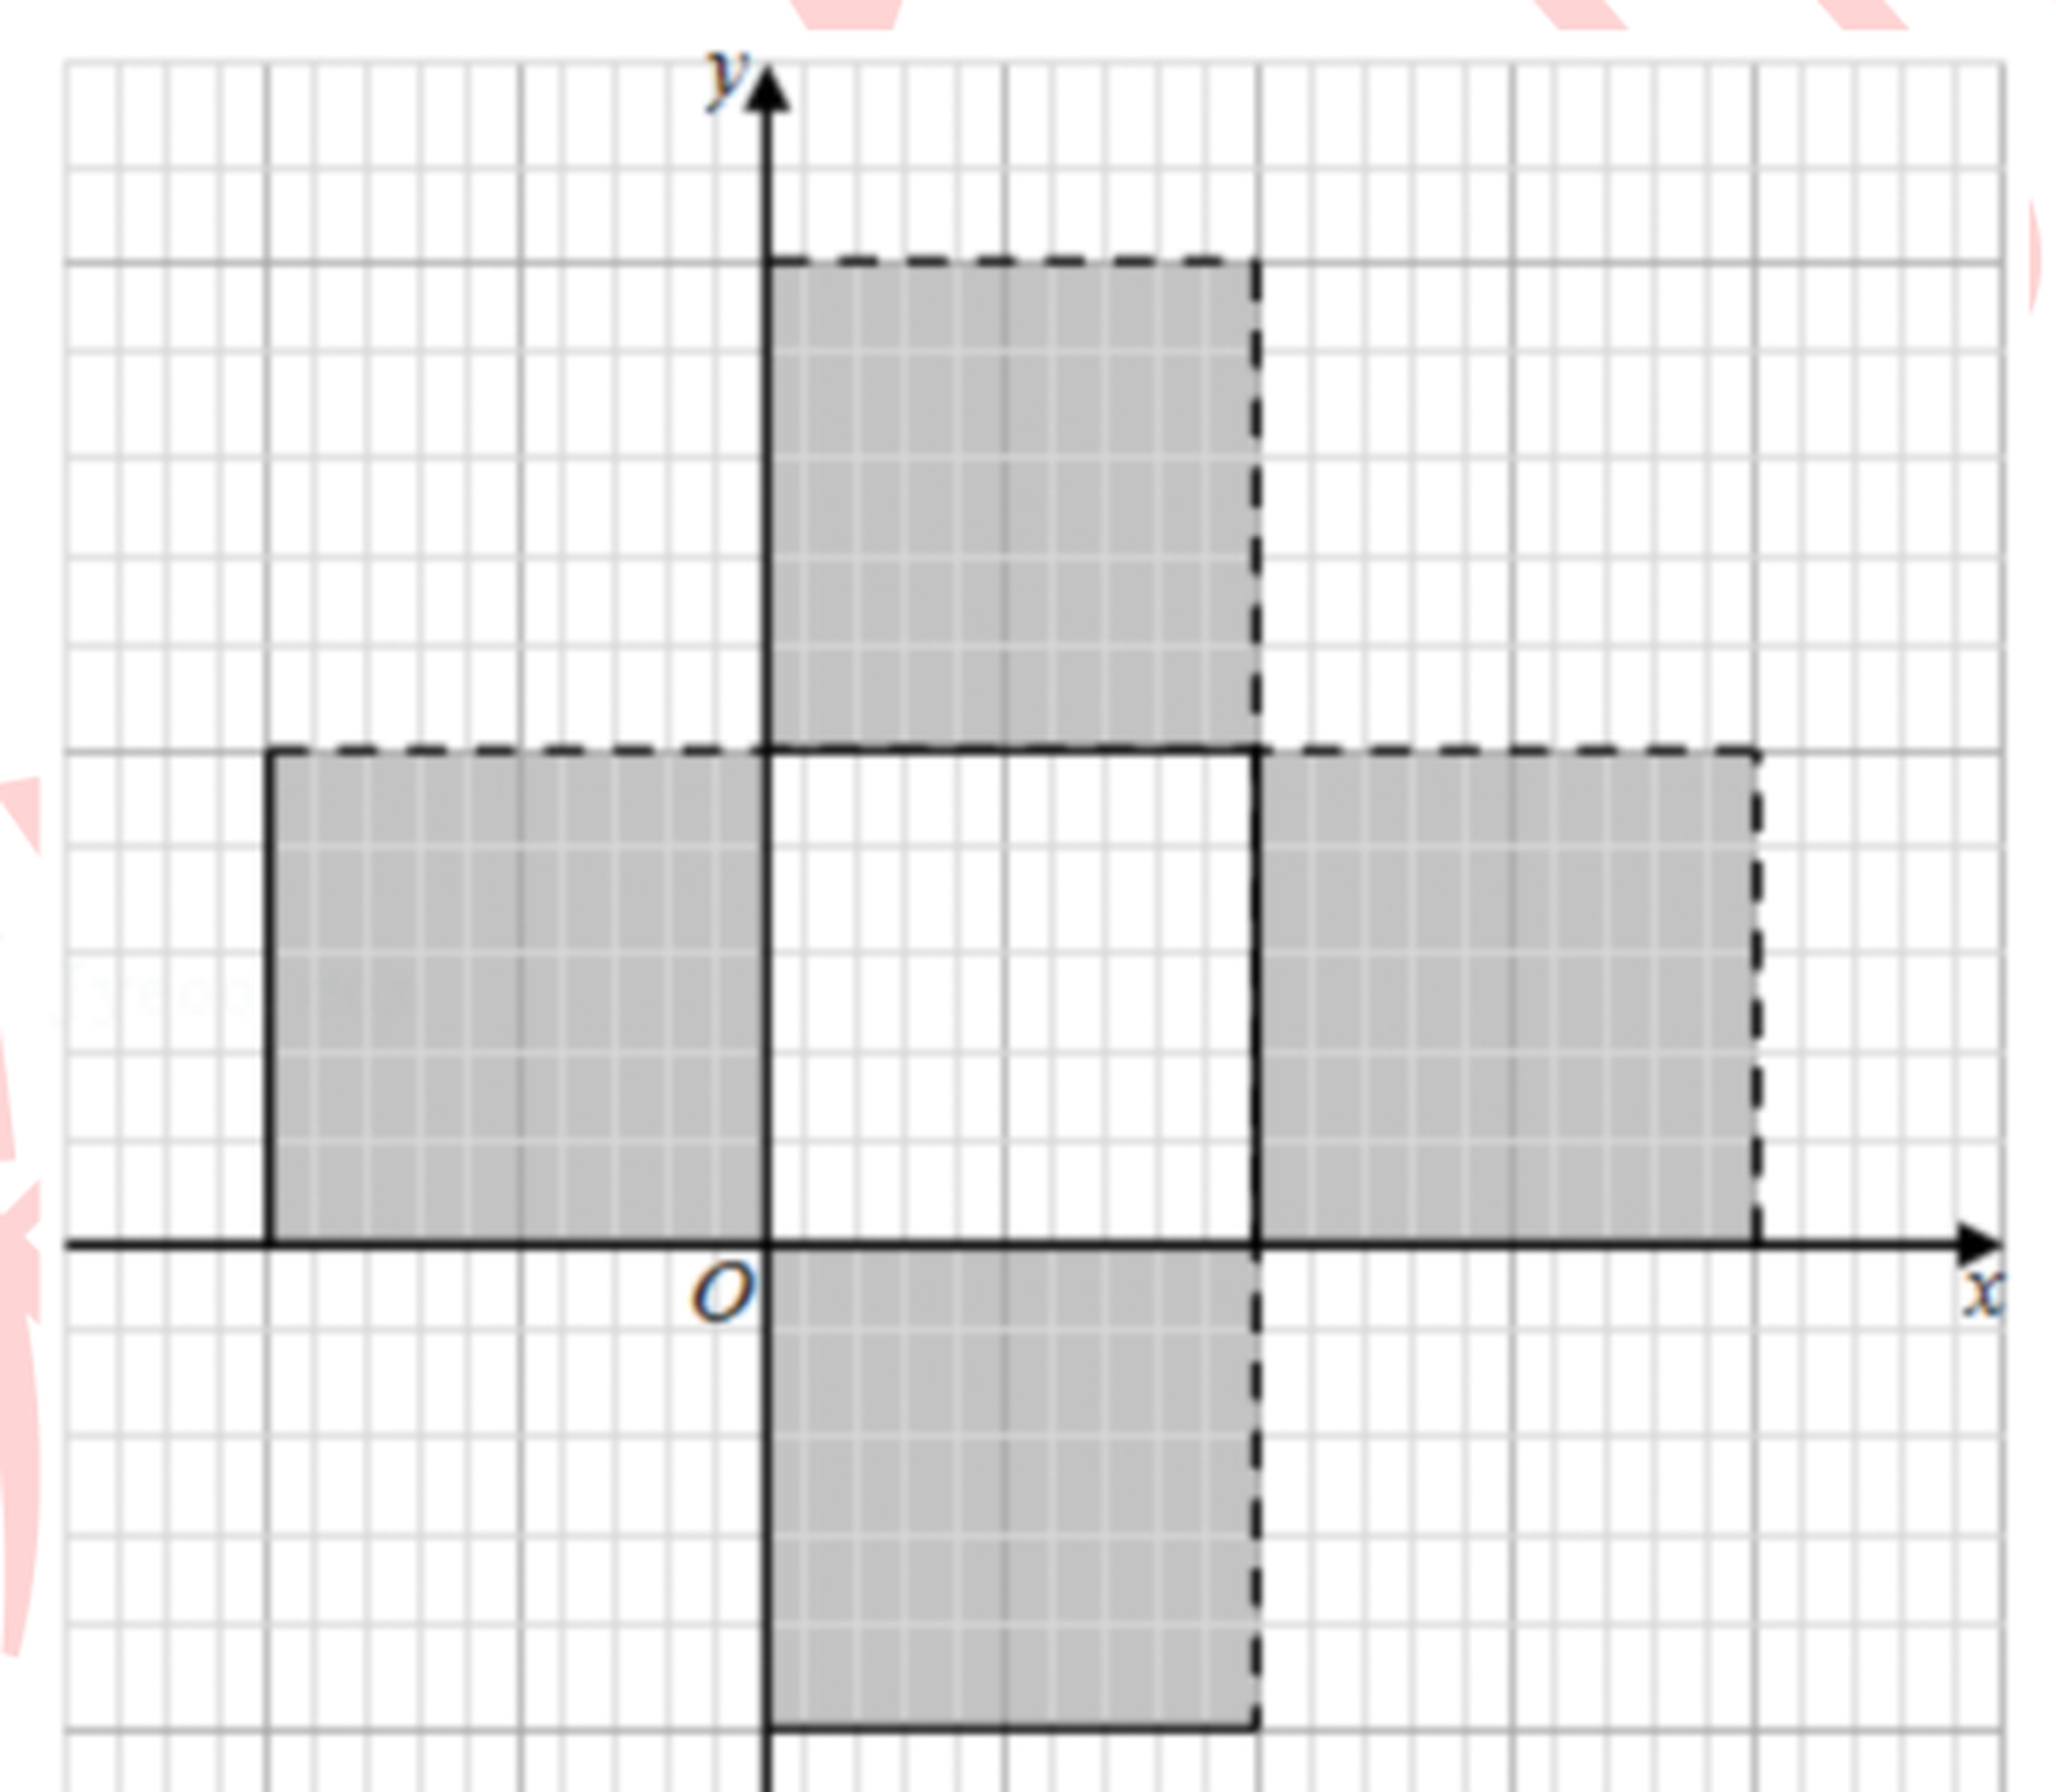
\includegraphics[width=0.38\textwidth]{figures/plane_grid_4squares_h39.png}
\end{center}
\step{总面积为 $1\times4=4$.}
\solend

\fi

\item 关于 $x$ 的不等式 $ax^2+bx+c>0$ 的解集为 $\{x\mid x<\beta\text{ 或 }x>\gamma\}(0<\beta<\gamma)$，
则不等式 $a(x^2+1)+b(x-1)+c>2ax$ 的解集为 \blankline[4.4em].

\ans{$(-\infty,\beta+1)\cup(\gamma+1,+\infty)$}

\ifanswer
\solbegin
\step{由题意得 $\beta$、$\gamma$ 为方程 $ax^2+bx+c=0$ 的两根且 $a>0$，}
\step{则 $\beta+\gamma=-\dfrac ba$，$\beta\gamma=\dfrac ca$，故 $b=-a(\beta+\gamma)$，$c=\beta\gamma a$，}
\step{则不等式可化为 $a(x^2+1)-a(\beta+\gamma)(x-1)+\beta\gamma a>2ax$，}
\step{因为 $a>0$，所以 $x^2+1-(\beta+\gamma)(x-1)+\beta\gamma>2x$，}
\step{即 $x^2-(\beta+\gamma+2)x+(\beta+\gamma+\beta\gamma+1)>0$，所以 $(x-\beta-1)(x-\gamma-1)>0$，}
\step{解得 $x<\beta+1$ 或 $x>\gamma+1$，所以不等式解集为 $(-\infty,\beta+1)\cup(\gamma+1,+\infty)$.}
\solend

\fi

\end{enumerate}

\bigsec{二、选择题}

\begin{enumerate}
\setcounter{enumi}{12}

\item 设 $a<b<0$，则下列不等式中不成立的是\mbox{（\quad）}

\keepwithprev
A. $\dfrac1a>\dfrac1b$\qquad B. $\dfrac{1}{a-b}>\dfrac1a$\qquad C. $|a|>-b$\qquad D. $\sqrt{-a}>\sqrt{-b}$

\ans{$B$}

\ifanswer
\solbegin
\step{令 $a=-2$，$b=-1$，}
\step{A、$-\dfrac12>-1$，正确；B、$-1<-\dfrac12$，故 B 错误；C、$2>1$，正确；}
\step{D、$\sqrt2>1$，正确；故选 B.}
\solend

\fi

\item 设实数集 $\R$ 为全集，集合 $P=\{x\mid f(x)=0\}$，$Q=\{x\mid g(x)=0\}$，$H=\{x\mid h(x)=0\}$，
则方程 $\dfrac{f^2(x)+g^2(x)}{h(x)}=0$ 的解集是\mbox{（\quad）}

\keepwithprev
A. $P\cap Q\cap\overline{H}$\qquad B. $P\cap Q$\qquad C. $P\cap Q\cap H$\qquad D. $P\cap Q\cup H$

\ans{$A$}

\ifanswer
\solbegin
\step{方程 $\dfrac{f^2(x)+g^2(x)}{h(x)}=0$ 等价于 $\begin{cases}f(x)=0\\ g(x)=0\\ h(x)\neq0\end{cases}$，}
\step{又因为 $P=\{x\mid f(x)=0\}$，$Q=\{x\mid g(x)=0\}$，$H=\{x\mid h(x)=0\}$，}
\step{所以方程 $\dfrac{f^2(x)+g^2(x)}{h(x)}=0$ 的解集是 $P\cap Q\cap\overline{H}$，故选 A.}
\solend

\fi

\item 设全集 $U$，在下列条件中，是 $B\sub A$ 的充要条件的有\mbox{（\quad）}

\keepwithprev
% 注：原卷此行 ② 与 ③ 之间**漏排分隔号**（①、③ 后都有「；」，② 后没有）；
%     本稿照录未补，见文件头「原卷笔误/存疑」⑩。
①$A\cup B=A$；\qquad ②$\overline{A}\cap B=\varnothing$\qquad ③$\overline{A}\sub\overline{B}$；\qquad ④$A\cup\overline{B}=U$

\keepwithprev
A. $1$ 个\qquad B. $2$ 个\qquad C. $3$ 个\qquad D. $4$ 个

\ans{$D$}

\item 已知集合 $M=\{x\mid x\in\N,0<x\leqslant15\}$，$A_1$、$A_2$、$A_3$ 满足：①$A_1\cup A_2\cup A_3=M$；
②每个集合都恰有 $5$ 个元素. 集合 $A_i(i=1,2,3)$ 中最大元素与最小元素之和称为 $A_i$ 的特征数，
记为 $X_i(i=1,2,3)$，则 $X_1+X_2+X_3$ 的值不可能为\mbox{（\quad）}

\keepwithprev
A. $37$\qquad B. $39$\qquad C. $48$\qquad D. $57$

\ans{$A$}

\ifanswer
\solbegin
\step{因为集合 $M=\{x\mid x\in\N,0<x\leqslant15\}=\{1,2,3,\cdots,15\}$，}
\step{又因为集合 $A_1$、$A_2$、$A_3$ 中，每个集合恰有 $5$ 个元素，}
\step{且 $A_1\cup A_2\cup A_3=M$ 有 $15$ 个元素，所以集合 $A_1$、$A_2$、$A_3$ 中没有重复元素，}
\step{因为 $1$ 是集合 $M$ 中数值最小的元素，$15$ 是集合 $M$ 中数值最大的元素，}
\step{所以在 $A_i$ 的特征数构成中，必有 $1$ 和 $15$，不妨设 $1\in A_1$，$15\in A_1$，}
% 注：原卷本行（与下面「最小」那句）在「集合」后的角标是**数字 $1$**（同句 $X_1$ 的角标同形），
%     而非上一行「$A_i$ 的特征数构成」里的斜体 $A_i$——原卷两种下标并存，本稿照录、不归一，
%     见文件头「原卷笔误/存疑」⑬。
\step{要使 $X_1+X_2+X_3$ 最大，则应该在集合 $A_1$ 中首先放置数值较小的元素，}
\step{即 $A_1=\{1,2,3,4,15\}$，所以 $5$ 与 $14$ 是剩下元素中数值最小或最大的元素，}
\step{同理，不妨设 $5\in A_2$，$14\in A_2$，接着在 $A_2$ 中再次放置数值较小的元素，}
\step{即 $A_2=\{5,6,7,8,14\}$，则 $A_3=\{9,10,11,12,13\}$，}
\step{此时 $X_1+X_2+X_3$ 有最大值为 $1+15+5+14+9+13=57$，}
\step{即 $X_1+X_2+X_3\leqslant57$；}
% 注：同上一处——原卷此行角标是**数字 $1$**（$A_1$），本稿照录，未与「$A_i$」归一。
\step{要使 $X_1+X_2+X_3$ 最小，则在集合 $A_1$ 中首先放置数值较大的元素，}
\step{即 $A_1=\{1,12,13,14,15\}$，所以 $2$ 与 $11$ 是剩下元素中数值最小或最大的元素，}
\step{同理，不妨设 $2\in A_2$，$11\in A_2$，接着在 $A_2$ 中再次放置数值较大的元素，}
\step{即 $A_2=\{2,8,9,10,11\}$，则 $A_3=\{3,4,5,6,7\}$，}
\step{此时 $X_1+X_2+X_3$ 有最小值为 $1+15+2+11+3+7=39$，}
\step{即 $X_1+X_2+X_3\geqslant39$，}
\step{综上，$39\leqslant X_1+X_2+X_3\leqslant57$，故选 A.}
\solend

\fi

\end{enumerate}

\bigsec{三、解答题}

\begin{enumerate}
\setcounter{enumi}{16}

% 注：原卷首句「由数 $y=-x^2+ax-1=-x+3$」中的「由数」显系「由」或「由函数」之误；末段
%     的两处分类讨论与结论自相矛盾（详见文件头「笔误/存疑」④）。本稿一律照录，未改。
\item 命题 $p$：函数 $y=-x^2+ax-1$ 与 $y=-x+3$ 图象交点的横坐标均为负值，
命题 $q$：关于 $x$ 的方程 $2(1-x)a+(x^2-10x-3)=0$ 的两个根，一个大于 $3$，另一个小于 $3$；
若命题 $p$ 和命题 $q$ 中有且仅有一个是真命题，求 $a$ 的取值范围.

\ans{$\R$}

\ifanswer
\solbegin
\step{由数 $y=-x^2+ax-1=-x+3$ 得 $x^2-(a+1)x+4=0$，}
\step{若横坐标均为负值，则满足 $\begin{cases}\Delta=(a+1)^2-16\geqslant0\\ x_1x_2=4>0\\ x_1+x_2=a+1<0\end{cases}$
得 $\begin{cases}a\geqslant3\text{ 或 }a\leqslant-5\\ a<-1\end{cases}$，得 $a\leqslant-5$，}
\step{即 $p:a\leqslant-5$，}
\step{若方程 $2(1-x)a+(x^2-10x-3)=0$ 的两个根，一个大于 $3$，另一个小于 $3$；}
\step{设 $f(x)=2(1-x)a+(x^2-10x-3)$，则 $f(3)<0$，即 $-4a-24<0$，}
\step{得 $a>-6$，即 $q:a>-6$，}
\step{因为命题 $p$ 和命题 $q$ 中有且仅有一个是真命题，}
\step{若 $p$ 真 $q$ 假，则 $\begin{cases}a\leqslant-5\\ a>-6\end{cases}$，得 $a\in\R$，}
\step{若 $p$ 假 $q$ 真，则 $\begin{cases}a>-5\\ a\leqslant-6\end{cases}$，此时 $a$ 无解，}
\step{综上，实数 $a$ 的取值范围是 $\R$.}
\solend

\fi

\ansspace[8]

\item 设全集是实数集 $\R$，$A=\left\{x\mid\dfrac{1-2x}{x-3}\geqslant0\right\}$，$B=\{x\mid x^2+a\leqslant0\}$.

\begin{enumerate}[label=(\arabic*)]

\item 当 $a=-4$ 时，求 $A\cup B$；

\item 若 $\overline{A}\cap B=B$，求实数 $a$ 的取值范围.

\end{enumerate}

\ans{（1）$\{x\mid-2\leqslant x<3\}$；（2）$\left(-\dfrac14,+\infty\right)$}

\ifanswer
\solbegin
\stepm{(1)}{$A=\left\{x\mid\dfrac{1-2x}{x-3}\geqslant0\right\}=\left\{x\mid\dfrac12\leqslant x<3\right\}$，$B=\{x\mid x^2+a\leqslant0\}$.}
\step{当 $a=-4$ 时，$B=\{x\mid-2\leqslant x\leqslant2\}$，所以 $A\cup B=\{x\mid-2\leqslant x<3\}$.}
\stepm{(2)}{$\overline{A}=\left\{x\mid x\geqslant3\text{ 或 }x<\dfrac12\right\}$，$B=\{x\mid x^2+a\leqslant0\}$.}
\step{由 $\overline{A}\cap B=B$，得 $B\sub\overline{A}$，}
\step{则当 $a>0$ 时，$B=\varnothing$，满足 $B\sub\overline{A}$，则 $a>0$ 成立，}
\step{则当 $a=0$ 时，$B=\{0\}$，满足 $B\sub\overline{A}$，则 $a=0$ 成立，}
\step{当 $a<0$ 时，$B=\{x\mid-\sqrt{-a}\leqslant x<\sqrt{-a}\}$，}
\step{得 $\sqrt{-a}<\dfrac12$，即 $-\dfrac14<a<0$，}
\step{综上，实数 $a$ 的取值范围是 $\left(-\dfrac14,+\infty\right)$.}
\solend

\fi

\ansspace[6]

\item 设集合 $A=\{x\mid ax^2+2x+1=0,a\in\R\}$.

\begin{enumerate}[label=(\arabic*)]

\item 当 $A$ 中元素个数为 $1$ 时，求：$a$ 和 $A$；

\item 当 $A$ 中元素个数至少为 $1$ 时，求：$a$ 的取值范围；

\item 求：$A$ 中各元素之和.

\end{enumerate}

\ans{（1）$a=0$ 时 $A=\left\{-\dfrac12\right\}$，$a=1$ 时 $A=\{-1\}$；（2）$(-\infty,1]$；
（3）$a=0$ 时和为 $-\dfrac12$，$a<1$ 且 $a\neq0$ 时和为 $-\dfrac2a$，$a=1$ 时和为 $-1$，$a>1$ 时 $A$ 中无元素}

\ifanswer
\solbegin
\stepm{(1)}{集合 $A=\{x\mid ax^2+2x+1=0,a\in\R\}$，$A$ 中元素个数为 $1$，}
\step{所以 $a=0$ 或 $\begin{cases}a\neq0\\ \Delta=4-4a=0\end{cases}$，解得 $a=0$，$A=\left\{-\dfrac12\right\}$ 或 $a=1$，$A=\{-1\}$.}
\stepm{(2)}{当 $A$ 中元素个数至少为 $1$ 时，$a=0$ 或 $\begin{cases}a\neq0\\ \Delta=4-4a\geqslant0\end{cases}$，解得 $a\leqslant1$，}
\step{所以 $a$ 的取值范围是 $(-\infty,1]$.}
\stepm{(3)}{当 $a=0$ 时，$A$ 中元素之和为 $-\dfrac12$；}
\step{当 $a<1$ 且 $a\neq0$ 时，$A$ 中元素之和为 $-\dfrac2a$；}
\step{当 $a=1$ 时，$A$ 中元素之和为 $-1$；}
\step{当 $a>1$ 时，$A$ 中无元素.}
\solend

\fi

\ansspace[8]

\item 设 $k$ 是正整数，集合 $A$ 至少有两个元素，且 $A\sub\N^*$. 如果对于 $A$ 中的任意两个不同的
元素 $x$、$y$，都有 $|x-y|\neq k$，则称 $A$ 具有性质 $P(k)$.

\begin{enumerate}[label=(\arabic*)]

\item 试判断集合 $B=\{1,2,3,4\}$ 和 $C=\{1,4,7,10\}$ 是否具有性质 $P(2)$？并说明理由；

\item 若集合 $A=\{a_1,a_2,\cdots,a_{12}\}\sub\{1,2,\cdots,20\}$，求证：$A$ 不可能具有性质 $P(3)$；

\item 若集合 $A\sub\{1,2,\cdots,2023\}$，且同时具有性质 $P(4)$ 和 $P(7)$，求集合 $A$ 中元素个数的
最大值.

\end{enumerate}

\ans{（1）$B$ 不具有性质 $P(2)$，$C$ 具有性质 $P(2)$；（2）见解析；（3）$920$}

\ifanswer
\solbegin
\stepm{(1)}{因为 $B=\{1,2,3,4\}$，}
\step{又 $1\in\N^*$，$2\in\N^*$，$3\in\N^*$，$4\in\N^*$，但 $|4-2|=2$，}
\step{所以集合 $B$ 不具有性质 $P(2)$，}
\step{因为 $C=\{1,4,7,10\}$，}
\step{又 $1\in\N^*$，$4\in\N^*$，$7\in\N^*$，$10\in\N^*$，}
\step{但 $|4-1|=3$，$|7-1|=6$，$|10-1|=9$，$|7-4|=3$，$|10-4|=6$，$|10-7|=3$，}
\step{所以集合 $C$ 具有性质 $P(2)$，}
\stepm{(2)}{将集合 $\{1,2,\cdots,20\}$ 中的元素分为如下 $11$ 个集合，}
% 注：原卷本行 $\{8,11\}$ 与 $\{9,12\}$ 之间的分隔号误用**句号**「.」（同行其余处皆逗号），
%     本稿照录、未改，见文件头「原卷笔误/存疑」⑪。
\step{$\{1,4\}$，$\{2,5\}$，$\{3,6\}$，$\{7,10\}$，$\{8,11\}$.$\{9,12\}$，$\{13,16\}$，$\{14,17\}$，$\{15,18\}$，}
\step{$\{19\}$，$\{20\}$，}
\step{所以从集合 $\{1,2,\cdots,20\}$ 中取 $12$ 个元素，则前 $9$ 个集合至少要选 $10$ 个元素，}
\step{所以必有 $2$ 个元素取自前 $9$ 个集合中的同一集合，即存在两个元素其差为 $3$，}
\step{所以 $A$ 不可能具有性质 $P(3)$；}
\stepm{(3)}{先说明连续 $11$ 项中集合 $A$ 中最多选取 $5$ 项，}
\step{以 $1,2,3,\cdots,11$ 为例.}
\step{构造抽屉 $\{1,8\}$，$\{2,9\}$，$\{3,10\}$，$\{4,11\}$，$\{5\}$，$\{6\}$，$\{7\}$.}
\step{①$5$、$6$、$7$ 同时选，因为具有性质 $P(4)$ 和 $P(7)$，}
\step{所以选 $5$ 则不选 $1$、$9$；选 $6$ 则不选 $2$、$10$；选 $7$ 则不选 $3$、$11$；}
% 注：原卷此步推理不严——「只剩 $4$、$8$」但两数相差 $4$、不能同选，该情形实际最多只能取 $4$ 个；
%     末句「不超过 $5$ 个」的结论仍成立。本稿照录，见文件头「原卷笔误/存疑」⑫。
\step{则只剩 $4$、$8$；故 $1,2,3,\cdots,11$ 中属于集合 $A$ 的元素个数不超过 $5$ 个.}
\step{②$5$、$6$、$7$ 选 $2$ 个，}
\step{若只选 $5$、$6$，则 $1$、$2$、$9$、$10$、$7$ 不可选，又 $\{4,11\}$ 只能选一个元素，}
\step{$3$、$8$ 可以选，故 $1,2,3,\cdots,11$ 中属于集合 $A$ 的元素个数不超过 $5$ 个.}
\step{若选 $5$、$7$，则只能从 $2$、$4$、$8$、$10$ 中选，但 $4$、$8$ 不能同时选，}
\step{故 $1,2,3,\cdots,11$ 中属于集合 $A$ 的元素个数不超过 $5$ 个.}
\step{若选 $6$、$7$，则 $2$、$3$、$10$、$11$、$5$ 不可选，又 $\{1,8\}$ 只能选一个元素，}
\step{$4$、$9$ 可以选，故 $1,2,3,\cdots,11$ 中属于集合 $A$ 的元素个数不超过 $5$ 个.}
\step{③$5$、$6$、$7$ 中只选 $1$ 个，}
\step{又四个集合 $\{1,8\}$，$\{2,9\}$，$\{3,10\}$，$\{4,11\}$ 每个集合至多选 $1$ 个元素，}
\step{故 $1,2,3,\cdots,11$ 中属于集合 $A$ 的元素个数不超过 $5$ 个.}
\step{由上述①②③得，连续 $11$ 项自然数中属于集合 $A$ 的元素至多只有 $5$ 个，}
\step{如取 $1$、$4$、$6$、$7$、$9$.}
\step{因为 $2023=183\times11+10$，则把每 $11$ 个连续自然数分组，}
\step{前 $183$ 组每组至多选取 $5$ 项；}
\step{从 $2014$ 开始，最后 $10$ 个数至多选取 $5$ 项，}
\step{故集合 $A$ 的元素最多有 $184\times5=920$ 个.}
\step{给出如下选取方法：从 $1,2,3,\cdots,11$ 中选取 $1$、$4$、$6$、$7$、$9$；}
\step{然后在这 $5$ 个数的基础上每次累加 $11$，构造 $183$ 次.}
\step{此时集合 $A$ 的元素为 $1$，$4$，$6$，$7$，$9$；$12$，$15$，$17$，$18$，$20$；$23$，$26$，$28$，$29$，$31$；
$\cdots$；$2014$，$2017$，$2019$，$2020$，$2022$，共 $920$ 个元素.}
\step{经检验得该集合符合要求，故集合 $A$ 的元素最多有 $920$ 个.}
\solend

\fi

\ansspace[10]

\end{enumerate}

\bigsec{附加题}

\begin{enumerate}
\setcounter{enumi}{20}

\item 若规定集合 $M=\{a_1,a_2,\cdots,a_n\}$（$n\in\N^*$）的子集 $\{a_{i_1},a_{i_2},\cdots,a_{i_m}\}$（$m\in\N^*$）
为 $M$ 的第 $k$ 个子集，其中 $k=2^{i_1-1}+2^{i_2-1}+\cdots+2^{i_m-1}$，则 $M$ 的第 $25$ 个子集是 \blankline[4.4em].

\ans{$\{a_1,a_4,a_5\}$}

\ifanswer
\solbegin
\step{由题意得 $M$ 的第 $k$ 个子集，且 $k=2^{i_1-1}+2^{i_2-1}+\cdots+2^{i_m-1}$，}
\step{又 $25=2^0+2^3+2^4=2^{1-1}+2^{4-1}+2^{5-1}$，所以 $M$ 的第 $25$ 个子集是 $\{a_1,a_4,a_5\}$.}
\solend

\fi

% 注：原卷在 $x=1$、$y=2$、$z=3$ 时把 $B=\{x,y\}$ 印作 $\{1,3\}$（应为 $\{1,2\}$），
%     照录未改，见文件头「笔误/存疑」⑥。
\item 用 $|S|$ 表示集合 $S$ 中的元素的个数，设 $A$、$B$、$C$ 为集合，称 $(A,B,C)$ 为有序三元组.
如果集合 $A$、$B$、$C$ 满足 $|A\cap B|=|B\cap C|=|C\cap A|=1$，且 $A\cap B\cap C=\varnothing$，
则称有序三元组 $(A,B,C)$ 为最小相交. 由集合 $\{1,2,3\}$ 的子集构成的所有有序三元组中，
最小相交的有序三元组的个数为 \blankline[4.4em].

\ans{$6$}

\ifanswer
\solbegin
\step{因为 $|A\cap B|=|B\cap C|=|C\cap A|=1$，}
\step{所以设 $A\cap B=\{x\}$，$B\cap C=\{y\}$，$C\cap A=\{z\}$，}
% 图在【解析】内（仅答案版出），取原卷截图（10.png，2560×3620）右栏，4× LANCZOS 放大。
\begin{center}
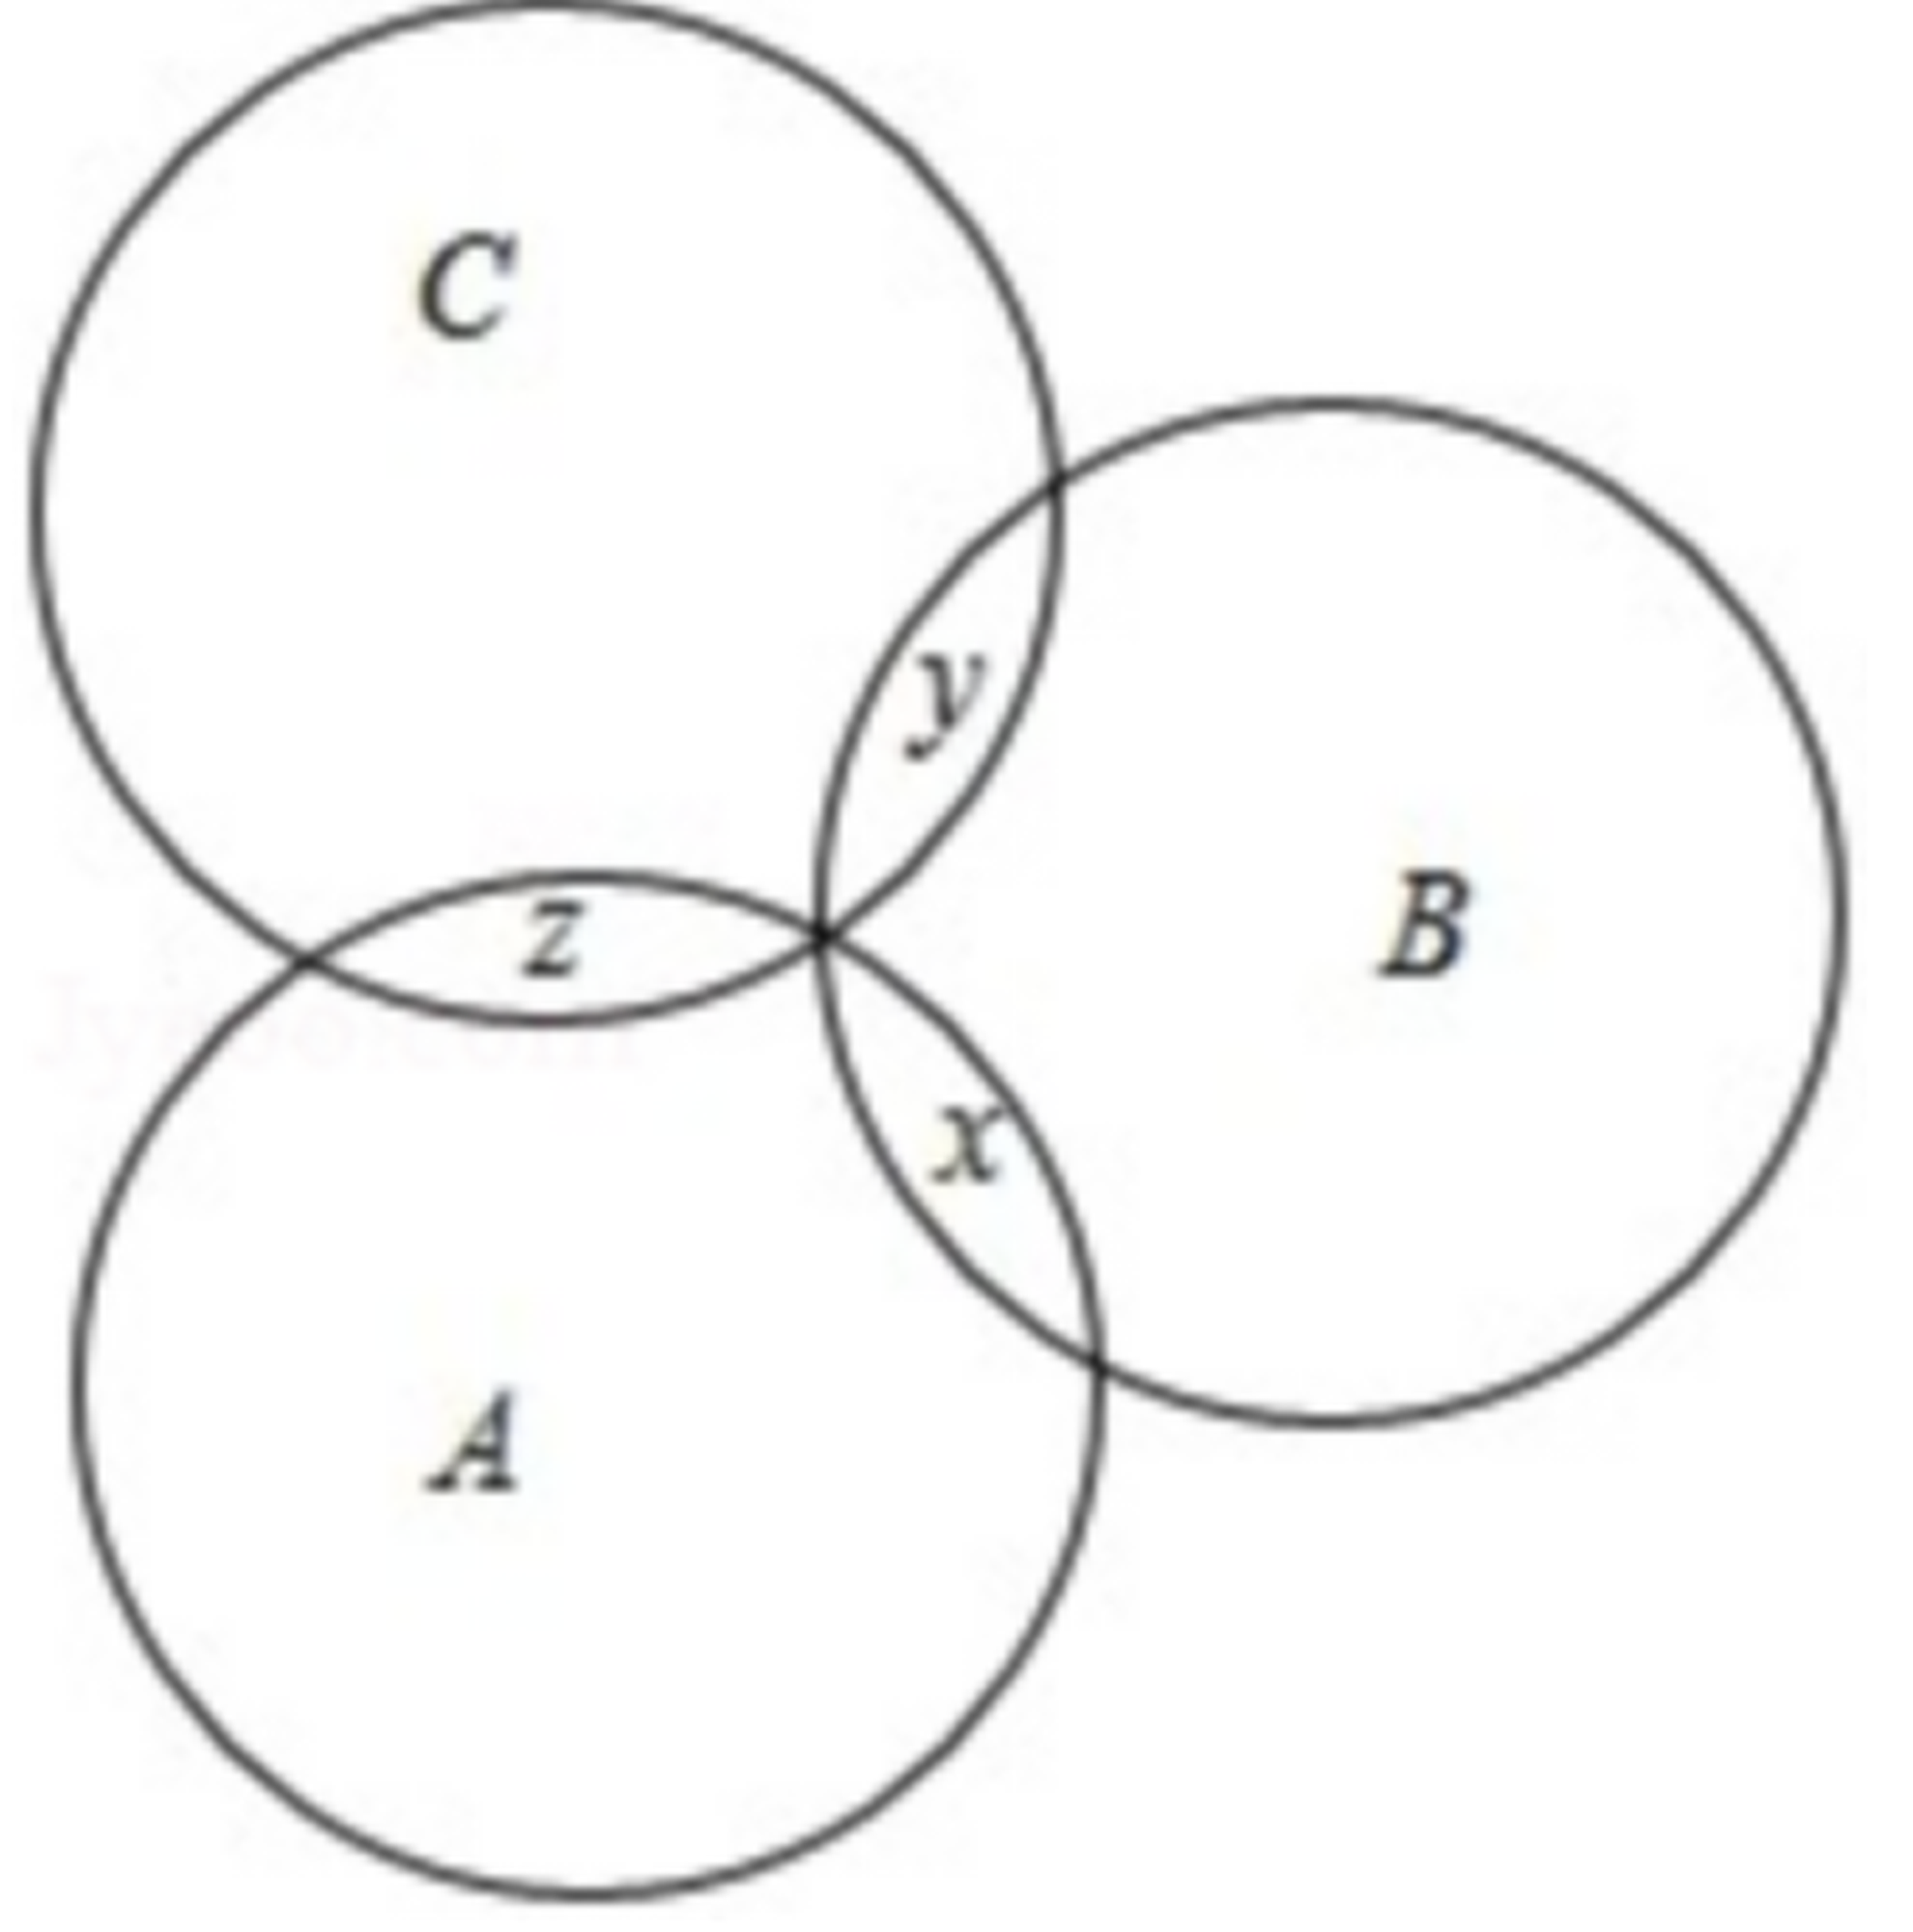
\includegraphics[width=0.30\textwidth]{figures/venn_ABC_x_y_z_h39.png}
\end{center}
\step{因为 $|A\cap B|=|B\cap C|=|C\cap A|=1$，且 $x$、$y$、$z\in\{1,2,3\}$，}
\step{所以集合 $A=\{x,z\}$，$B=\{x,y\}$，$C=\{z,y\}$，}
\step{若 $x=1$，$y=2$，$z=3$，则 $A=\{1,3\}$，$B=\{1,3\}$，$C=\{2,3\}$，}
\step{将 $1$，$2$，$3$ 进行全排列，有 $P_3^3=3\times2=6$ 个.}
\solend

\fi

\item 已知集合 $T=\{1,2,\cdots,2025\}$，对于 $T$ 的每一个非空子集的所有元素，计算它们乘积的倒数，
则所有这样倒数的和为 \blankline[4.4em].

\ans{$2025$}

\ifanswer
\solbegin
\step{集合 $T=\{1,2,\cdots,2025\}$ 的非空子集的个数为 $2^{2025}-1$，}
\step{这些子集中，每个元素的乘积分别为}
\step{$1,2,3,\cdots,2025,1\times2,1\times3,\cdots,1\times2025,\cdots,1\times2\times3\times\cdots\times2025$，}
\step{每项都可以看作是从 $1,2,3,\cdots,2025$ 中选择若干项的乘积，}
\step{$1+\dfrac12+\cdots+\dfrac{1}{2025}+\dfrac{1}{1\times2}+\dfrac{1}{1\times3}+\cdots+\dfrac{1}{2024\times2025}
+\cdots+\dfrac{1}{1\times2\times\cdots\times2025}$}
\step{$=(1+1)\left(1+\dfrac12\right)\cdots\left(1+\dfrac{1}{2025}\right)-1
=2\times\dfrac32\times\dfrac43\times\cdots\times\dfrac{2026}{2025}-1=2025$.}
\solend

\fi

% 第 24 题是压轴题，题干较长；试卷版在它之前量一次页高，尽量不与前文分家（照全稿成例）。
\ansneed{5cm}
% 注：原卷【解析】①③ 两步把 $f(x)$ 印作 $f[x[x]]$，显系笔误，照录未改，见文件头「笔误/存疑」⑦。
\item 若 $X$ 是一个集合，$T$ 是一个以 $X$ 的某些子集为元素的集合，且满足：①$X$ 属于 $T$，
$\varnothing$ 属于 $T$；②$T$ 中任意多个元素的并集属于 $T$；③$T$ 中任意多个元素的交集属于 $T$.
则称 $T$ 是集合 $X$ 上的一个拓扑. 已知函数 $f(x)=[x[x]]$，其中 $[x]$ 表示不大于 $x$ 的最大整数，
当 $x\in(0,n]$，$n\in\N^*$ 时，函数 $f(x)$ 值域为集合 $A_n$，则集合 $A_2$ 上的含有 $4$ 个元素的
拓扑 $T$ 的个数为 \blankline[4.4em].

\ans{$9$}

\ifanswer
\solbegin
\step{由题意，$n=2$，故 $0<x\leqslant2$，}
\step{①当 $0<x<1$ 时，则 $[x]=0$，所以 $f[x[x]]=0$，}
\step{②当 $x=1$ 时，$[x]=1$ 显然 $f(1)=1$，}
\step{③当 $1<x<2$ 时，$[x]=1$，所以 $f[x[x]]=[x]=1$，}
\step{④当 $x=2$ 时，$f(2)=4$，}
\step{所以 $A_2=\{0,1,4\}$，}
\step{因为 $T$ 中含有 $4$ 个元素，其中两个元素 $\varnothing$ 和 $A_2$，}
\step{$A_2=\{0,1,4\}$. 其它两个元素为 $A$、$B$，则
$\begin{cases}A\neq\varnothing\\ A\neq A_2\\ B\neq\varnothing\\ B\neq A_2\\ A\neq B\end{cases}$，}
\step{由对称性，不妨设 $1\leqslant|A|\leqslant|B|\leqslant2$，其中 $|A|$、$|B|$ 表示集合 $A$ 中元素的个数，}
\step{因为 $\begin{cases}A\cap B\in T\\ A\cup B\in T\end{cases}$，又 $|A|\leqslant|B|$，所以 $A\cap B=\varnothing$ 或 $A$，}
\step{若 $A\cap B=\varnothing$，则 $A\cup B$ 只能等于 $A_2$，}
\step{（若 $A\cup B=B$，则 $A\sub B$，则 $A\cap B=A=\varnothing$，矛盾）}
\step{则必有 $\begin{cases}|A|=1\\ |B|=2\end{cases}$，所以 $(A,B)$ 的个数 $\Leftrightarrow$ $A$ 的个数 $=3$ 种，}
\step{即 $\begin{cases}A=\{0\}\\ B=\{1,4\}\end{cases}$ 或 $\begin{cases}A=\{1\}\\ B=\{0,4\}\end{cases}$
或 $\begin{cases}A=\{4\}\\ B=\{0,1\}\end{cases}$；}
\step{若 $A\cap B=A\Leftrightarrow A\sub B$ 此时满足 $A\cup B=B$，}
\step{因为 $A\neq B$ 且 $1\leqslant|A|$ 且 $|B|\leqslant2$，所以 $\begin{cases}|A|=1\\ |B|=2\end{cases}$，}
\step{所以 $B$ 的选择共有 $C_3^2=3$ 种，则 $A$ 的个数有 $C_2^1$ 种，}
\step{所以 $(A,B)$ 的个数 $=2\times3=6$ 种.}
% 这六组「$A$／$B$」按原卷排作两行（前五个一行、第六个另起一行）；因五组并排时
% amsmath 的 cases 会为每组的第二列各留一枚 \quad，本行改排 \left\{\begin{matrix}…\end{matrix}\right.
% 以省下这枚 \quad（照 README「说明」记的高一07 成例），字形与 cases 相同。
\step{（这 $6$ 种是 $\left\{\begin{matrix}A=\{0\}\\ B=\{0,1\}\end{matrix}\right.$、
$\left\{\begin{matrix}A=\{1\}\\ B=\{0,1\}\end{matrix}\right.$、
$\left\{\begin{matrix}A=\{0\}\\ B=\{0,4\}\end{matrix}\right.$、
$\left\{\begin{matrix}A=\{4\}\\ B=\{0,4\}\end{matrix}\right.$、
$\left\{\begin{matrix}A=\{1\}\\ B=\{1,4\}\end{matrix}\right.$、}
\step{$\left\{\begin{matrix}A=\{4\}\\ B=\{1,4\}\end{matrix}\right.$）.}
\step{综上，$T$ 的个数为 $9$ 个.}
\solend

\fi

\end{enumerate}

\end{document}
"
% 紧凑版：xelatex "\def\iscompact{1}% 高一39_大同中学_周末作业4.1.tex
%   —— 高一上数学「2026-2027 年大同中学高一上周末作业 4.1」（试卷版/答案版）
% 试卷版：xelatex 高一39_大同中学_周末作业4.1.tex
% 答案版：xelatex "\def\isanswer{1}% 高一39_大同中学_周末作业4.1.tex
%   —— 高一上数学「2026-2027 年大同中学高一上周末作业 4.1」（试卷版/答案版）
% 试卷版：xelatex 高一39_大同中学_周末作业4.1.tex
% 答案版：xelatex "\def\isanswer{1}\input{高一39_大同中学_周末作业4.1.tex}"
% 紧凑版：xelatex "\def\iscompact{1}\input{高一39_大同中学_周末作业4.1.tex}"
%
% 原始材料是微信公众号图文（公众号「魔都数学加油站」连载「27学年高一 39」，署名「破晓」，
% 2026-09-26 21:29 发布，原文标题「27学年高一39——2026-2027年上海市大同中学高一上周末作业4.1」，
% 原文链接 https://mp.weixin.qq.com/s/HR2hIayXUXNi4zTs3PioiQ ），正文为 11 张 PNG 页。**同一篇里各页分辨率不一致**（2560×3620 与 4762×6735 两档混排：第 1、3、8、10 页为
% 2560×3620，第 2、4、5、6、7、9、11 页为 4762×6735）。原文本身就是一份**讲评版**——除第 15 题
% 外各题题下直接印【解析】（无单独的【答案】行），第 15 题的答案「D」直接印在题干末尾的括号内。
% 试题文字、答案与解析均照原卷录入，未改内容。卷面的粉色斜水印「魔都数学加油站」属水印，未录入。
%
% 卷首标题：原卷页首印作「2026-2027 年大同中学高一上周末作业 4.1」（**卷面标题行即带校名**，
% 年份区间按全稿惯例排 en dash，前缀照原卷保留「年」）。
%
% 篇幅与题号：卷面自「一、填空题」的**第 3 题**起编，终于「附加题」的**第 24 题**，共 22 题
% （填空 3—12、选择 13—16、解答 17—20、附加题 21—24）。第 1、2 题未在该文中发布——这是该
% 公众号连载讲评版的通例（高一02—高一09 等均自第 3 题起编，README「说明」已记），**不是截断**，
% 故本稿题号亦自 3 起。它与 高一40（大同中学 周末作业4.2）同属「周末作业 4」系列但**各自独立起编**
% （4.2 自第 3 题起、终于第 19 题），不是同一份试卷的两半。
%
% 与原卷的排版差异（均已在 README「说明」中交代）：
%   ① 原文自**第 3 题**起（第 1、2 题未在该文中发布），故本稿题号亦自 3 起，填空题以
%      \setcounter{enumi}{2} 起编；选择、解答、附加题三节各按上一节末号另设 \setcounter
%      （选择题 \setcounter{enumi}{12}、解答题 \setcounter{enumi}{16}、附加题 \setcounter{enumi}{20}）；
%   ② 原卷本就印有「一、填空题」「二、选择题」「三、解答题」三节标题，末节印作「附加题」
%      （**不带「四、」**，且题号 21—24 续前编、不另起），本稿照原卷分节，只把标题改排成全稿
%      统一的「大节标题」样式；
%   ③ 原卷是「讲评版」：除第 15 题外，各题题下均印【解析】（**全卷无一条独立的【答案】行**）；
%      第 15 题无解析，答案「D」直接印在题干末尾的括号内。本稿统一改为试卷版隐去、答案版以
%      \ans{}／\ifanswer 块给出，两版彻底分离；原卷写在【解析】末句的结果，本稿照 高一38
%      （同校同系列、同为讲评版）的成例另提为 \ans{}；
%   ④ 数集记号原卷两套并用：实数集作斜体的 $R$（第 7、11、14、17、18、19 题），整数集作斜体
%      $Z$（第 10 题），自然数集作斜体 $N$ 及 $N^*$（第 16、20、21、24 题），本稿按全稿惯例
%      统一写作 $\R$、$\Z$、$\N$、$\N^*$；
%   ⑤ 补集符号原卷两套并用：第 7 题作前缀式的 $C_U$（且题干称全集为 $I$，见「笔误/存疑」①），
%      第 14、15、18 题作上横线（$\overline{H}$、$\overline{A}$、$\overline{B}$），本稿照录、不归一
%      （前缀式写作 $\complement_U$，与 高一c／高一10 的成例一致）；
%   ⑥ 包含符号原卷两套并用：第 3 题作**无下划线**的 $\subset$，第 15、18、20、24 题作**带下划线**
%      的 $\sub$，本稿照录、不归一；
%   ⑦ 原卷填空的横线约两个字宽，本稿按全稿惯例统一排 \blankline[4.4em]；
%   ⑧ 第 7、11、22 题各有插图，取原卷截图、4× LANCZOS 放大（figures/venn_N_cap_CI_M_h39.png、
%      figures/plane_grid_4squares_h39.png、figures/venn_ABC_x_y_z_h39.png）；第 7 题的 Venn 属
%      **题干**（试卷版、答案版都出），第 11、22 题的图在【解析】内（仅答案版出）。第 7 题图
%      左下、第 11 题图的上／左／右边缘带进极淡的原卷粉色水印残影——照全稿「插图直接取自
%      原卷截图、不用 TikZ 重绘、不修图」的体例保留（再裁会切到坐标轴与 $x$、$y$、$O$ 标注）；
%   ⑨ 原卷并列的字母、数字（「$x_1,x_2$」「$a,b$」「$1,2,3,\cdots,11$」）多作半角逗号或不加标点，
%      本稿按全稿惯例改排顿号（$x_1$、$x_2$）或把数列并入行内公式；半角括号、逗号一律排全角，
%      数学式内部的标点照原样；
%   ⑩ 原卷未印副标题，本稿按**本卷实际内容**补出副标题「集合与常用逻辑用语」（依据见下条）。
%
% 副标题（\examtitlest 第二个参数）：本卷卷面未印副标题，由本稿补出，取值按 2026-09-26 起的
%   新口径「只用本卷实际内容的模块名」定为「集合与常用逻辑用语」。依据：全卷 22 题（第 3—24 题）中，
%   第 3、5、7、8、10、11、14、15、16、17、18、19、20、21、22、23、24 题共 17 题是集合的运算与
%   关系、子集／真子集、补集、集合新定义（「全食／偏食」、最小相交、拓扑、特征数）与集合计数，
%   以及命题与常用逻辑用语（第 3 题充要条件、第 5 题存在量词命题、第 17 题命题真假）；其余两题
%   第 4、6 考一元二次方程的根（韦达定理）与方程恒等，第 9、12、13 题是不等式（一元二次不等式组
%   的整数解、一元二次不等式解集、不等式的性质）——不等式合计 3/22，**不足全卷三分之一**，
%   故不并标「不等式」。
%
% 原卷笔误/存疑（均照抄原卷、未改，见源码中该处上方注释）：
%   ① 第 7 题题干称「全集 $I=R$」，而【解析】两处把补集写作 $C_U M$（下标作 $U$），前后记号不一；
%      本稿照录，未改；
%   ② 第 4 题【解析】两处把判别式印作 $\triangle=[2(m-1)^2-16m^2]$（方括号内首项漏了平方，
%      正确应作 $[2(m-1)]^2-16m^2$）；按其所判「$m=\frac12$ 时 $<0$、$m=-\frac12$ 时 $>0$」反推，
%      $[2(m-1)]^2-16m^2$ 在 $m=\frac12$ 时为 $-3<0$、在 $m=-\frac12$ 时为 $5>0$，与结论一致；
%      本稿照录；
%   ③ 第 9 题【解析】把方程组第二式印作 $1-2<-k\leqslant3$，按其结论 $-3\leqslant k<2$ 反推，
%      疑当作 $-2<-k\leqslant3$（原卷多一个「$1$」）；本稿照录；
%   ④ 第 17 题【解析】首句「由数 $y=-x^2+ax-1=-x+3$」中的「由数」显系「由」或「由函数」之误；
%      且末段「若 $p$ 真 $q$ 假…得 $a\in R$」「若 $p$ 假 $q$ 真…此时 $a$ 无解」与结论「$a$ 的取值范围
%      是 $R$」自相矛盾（按 $p:a\leqslant-5$、$q:a>-6$，$p$ 真 $q$ 假应为 $a\leqslant-6$，$p$ 假 $q$ 真
%      应为 $a>-5$，合起来是 $a\leqslant-6$ 或 $a>-5$，并非 $R$）；本稿一律照录，未按正确解法改写；
%   ⑤ 第 18 题【解析】(2) 把 $B=\{x\mid x^2+a\leqslant0\}$（$a<0$）印作右端开的
%      $\{x\mid-\sqrt{-a}\leqslant x<\sqrt{-a}\}$（应为闭的「$\leqslant$」）；按其所判
%      $\sqrt{-a}<\frac12$ 反推，不影响结论；本稿照录；
%   ⑥ 第 22 题【解析】在 $x=1$、$y=2$、$z=3$ 时把 $B=\{x,y\}$ 印作 $\{1,3\}$（应为 $\{1,2\}$），
%      与本行前面「$B=\{x,y\}$」不合；本稿照录；
%   ⑦ 第 24 题【解析】①③ 两步把 $f(x)$ 印作 $f[x[x]]$，显系笔误；本稿照录。
%   ⑧ 第 8 题【解析】「即方程 $x^2+ax+b=x$，$x^2+(a-1)x+b=0$ **由**两个相等的实数根为 $4$」——
%      「由」当为「有」（「设…是…有」的杂糅）；本稿照录；
%   ⑨ 第 10 题：题设 $a\oplus b=b(a^2+b^2+1)$，而集合定义里含 $\dfrac{a\oplus b}{2b}$；$-2<a<b<2$、
%      $a$、$b\in\Z$ 时 $(a,b)=(-1,0)$ 也合条件、却使分母 $2b=0$，原卷解析仍代入该组并约去
%      $b$ 得 $x=1$（答案集恰好不变）；本稿照录；
%   ⑩ 第 15 题选项列里 ② 与 ③ 之间**漏排分隔号**（原卷作「② $\overline{A}\cap B=\varnothing$③
%      $\overline{A}\sub\overline{B}$；」——①、③ 后都有「；」，② 后没有）；本稿照录；
%   ⑪ 第 20(2) 把 $\{1,2,\cdots,20\}$ 分成的 11 个集合里，$\{8,11\}$ 与 $\{9,12\}$ 之间误用
%      **句号**「.」（同行其余处皆逗号）；本稿照录；
%   ⑫ 第 20(3)① 推理不严：原卷写「选 5 则不选 1、9；选 6 则不选 2、10；选 7 则不选 3、11；
%      则只剩 4、8」——但 4 与 8 相差 $4$、不能同选，该情形实际最多只能取 $4$ 个；末句结论
%      「不超过 $5$ 个」仍成立；本稿照录；
%   ⑬ 第 16 题【解析】两种下标并存：「所以在 $A_i$ 的特征数构成中」原卷作斜体 $A_i$，而
%      「要使 $X_1+X_2+X_3$ 最大（小），则（应）在集合 $A_1$ 中首先放置…」两处原卷作
%      **数字 $1$**（与同句 $X_1$ 的角标同形）；本稿照录、未归一。
%
% 图取原卷截图（依次见各处的 \includegraphics 前的注释），4× LANCZOS 放大。
\documentclass[a4paper,11pt]{article}
\usepackage{common}

\begin{document}

\examtitlest[3]{2026--2027 年大同中学高一上周末作业 4.1}{集合与常用逻辑用语}

\bigsec{一、填空题}

\begin{enumerate}
\setcounter{enumi}{2}

\item “$x\geqslant a$”是“$0<x<2$”的必要非充分条件，则实数 $a$ 的取值范围是 \blankline[4.4em].

\ans{$(-\infty,0]$}

\ifanswer
\solbegin
\step{因为 $x\geqslant a$ 是 $0<x<2$ 的必要非充分条件，所以 $(0,2)\subset[a,+\infty)$，所以 $a\leqslant0$，}
\step{则实数 $a$ 的取值范围是 $(-\infty,0]$.}
\solend

\fi

% 注：原卷$[2(m-1)^2-16m^2]$ 首项漏了平方（应为 $[2(m-1)]^2-16m^2$），照录未改，见文件头「笔误/存疑」②。
\item 若关于 $x$ 的方程 $x^2+2(m-1)x+4m^2=0$ 有两个实数根，且这两根互为倒数，则 $m=$ \blankline[4.4em].

\ans{$-\dfrac12$}

\ifanswer
\solbegin
\step{设 $x_1$、$x_2$ 是方程 $x^2+2(m-1)x+4m^2=0$ 有两个实数根，}
\step{则 $x_1x_2=4m^2=1$，解得 $m=\dfrac12$ 或 $m=-\dfrac12$，}
\step{又当 $m=\dfrac12$ 时，$\triangle=[2(m-1)^2-16m^2]<0$，舍去，}
\step{当 $m=-\dfrac12$ 时，$\triangle=[2(m-1)^2-16m^2]>0$，故 $m=-\dfrac12$.}
\solend

\fi

\item 已知命题：“存在 $x\in[1,2]$，使 $x^2+2x+a\geqslant0$”为真命题，则 $a$ 的取值范围是 \blankline[4.4em].

\ans{$a\geqslant-8$}

\ifanswer
\solbegin
\step{若存在 $x\in[1,2]$，使 $x^2+2x+a\geqslant0$，}
\step{则等价为存在 $x\in[1,2]$，使 $x^2+2x\geqslant-a$，}
\step{当存在 $x\in[1,2]$ 时，设 $y=x^2+2x=(x+1)^2-1$，则 $3\leqslant y\leqslant8$，}
\step{所以要使 $x^2+2x\geqslant-a$，则 $8\geqslant-a$，即 $a\geqslant-8$.}
\solend

\fi

\item 已知方程 $a(3x+2)+b(2x-3)=8x+3$ 有无穷多个解，则 $a:b=$ \blankline[4.4em].

\ans{$30:7$}

\ifanswer
\solbegin
\step{$a(3x+2)+b(2x-3)=(3a+2b)x+2a-3b=8x+3$ 有无穷多个解，}
\step{所以 $\begin{cases}3a+2b=8\\ 2a-3b=3\end{cases}$，解得 $a=\dfrac{30}{13}$，$b=\dfrac{7}{13}$，所以 $a:b=30:7$.}
\solend

\fi

% 注：原卷题干称「全集 $I=R$」，而【解析】两处把补集写作 $C_U M$（下标作 $U$），前后记号不一；
%     照录未改，见文件头「笔误/存疑」①。
\item 已知集合 $M=\{x\mid y=\sqrt{3-x^2}\}$，$N=\{x\mid-3\leqslant x\leqslant1\}$，全集 $I=\R$，
则图中阴影部分表示的集合为 \blankline[4.4em].

% 图取原卷截图（01.png，2560×3620）右栏，4× LANCZOS 放大。
\begin{center}
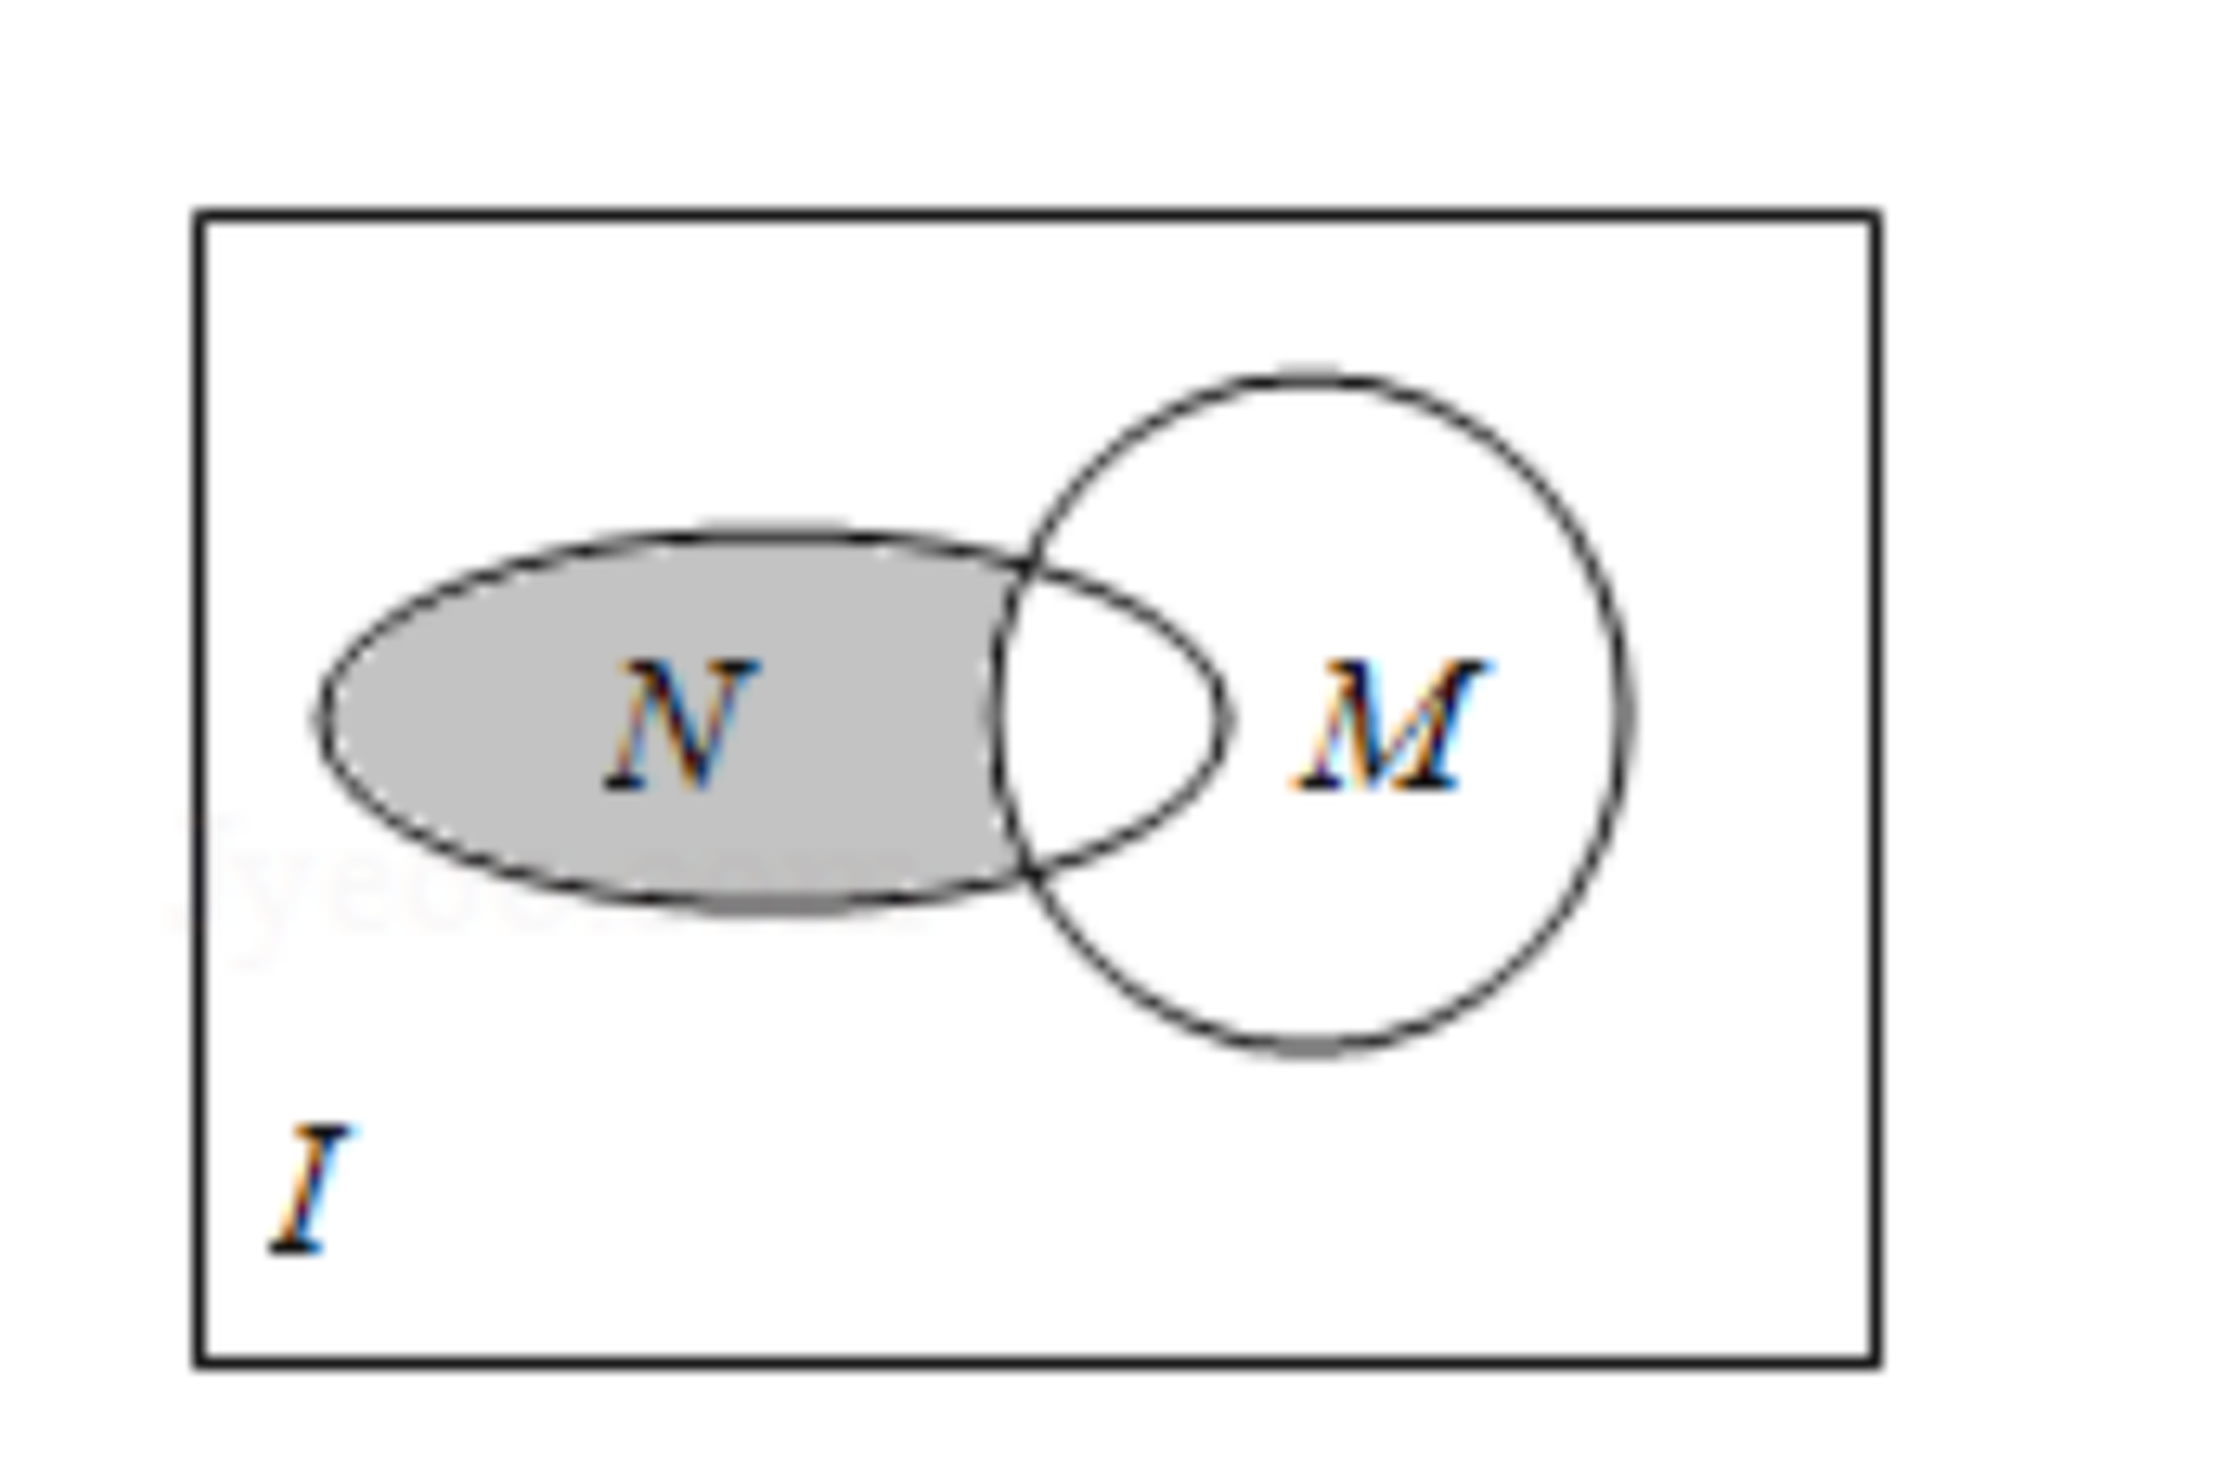
\includegraphics[width=0.30\textwidth]{figures/venn_N_cap_CI_M_h39.png}
\end{center}

\ans{$[-3,-\sqrt3)$}

\ifanswer
\solbegin
\step{阴影部分用集合表示为 $N\cap(\complement_UM)$.}
\step{则 $M=\{x\mid y=\sqrt{3-x^2}\}=\{x\mid3-x^2\geqslant0\}=\{x\mid-\sqrt3\leqslant x\leqslant\sqrt3\}$，}
\step{则 $\complement_UM=\{x\mid x>\sqrt3\text{ 或 }x<-\sqrt3\}$，$N=\{x\mid|x+1|\leqslant2\}=\{x\mid-3\leqslant x\leqslant1\}$，}
\step{则 $N\cap(\complement_UM)=\{x\mid-3\leqslant x<-\sqrt3\}$.}
\solend

\fi

\item 已知 $f(x)=x^2+ax+b$，集合 $\{x\mid f(x)=x\}=\{4\}$，将集合 $M=\{x\mid f(x)=4\}$ 用列举法表示 \blankline[4.4em].

\ans{$\{3,4\}$}

\ifanswer
\solbegin
\step{已知 $f(x)=x^2+ax+b$，集合 $\{x\mid f(x)=x\}=\{4\}$，}
% 注：原卷本行作「…$x^2+(a-1)x+b=0$ **由**两个相等的实数根为 $4$」——「由」当为「有」
%     （「设…是…有」的杂糅）；本稿照录未改，见文件头「原卷笔误/存疑」⑧。
\step{即方程 $x^2+ax+b=x$，$x^2+(a-1)x+b=0$ 由两个相等的实数根为 $4$，}
\step{所以 $\triangle=(a-1)^2-4b=0$，即 $x^2+(a-1)x+b=(x-4)^2$，所以 $b=16$，$a=-7$，}
\step{所以 $f(x)=x^2+ax+b=x^2-7x+16$，所以集合 $M=\{x\mid f(x)=4\}$，}
\step{即 $x^2-7x+16=4$，$x^2-7x+12=0$，故 $M=\{x\mid f(x)=4\}=\{3,4\}$.}
\solend

\fi

% 注：原卷方程组第二式印作 $1-2<-k\leqslant3$，按其结论 $-3\leqslant k<2$ 反推疑当作 $-2<-k\leqslant3$，
%     照录未改，见文件头「笔误/存疑」③。
\item 关于 $x$ 的不等式组 $\begin{cases}x^2-x-2>0\\ 2x^2+(2k+5)x+5k<0\end{cases}$ 的整数解的集合为 $\{-2\}$，
则实数 $k$ 的取值范围 \blankline[4.4em].

\ans{$-3\leqslant k<2$}

\ifanswer
\solbegin
\step{原不等式组即 $\begin{cases}(x-2)(x+1)>0\\ (x+k)(2x+5)<0\end{cases}$，整数解的集合为 $A$，若 $A=\{-2\}$，}
\step{则 $(-2+k)(2\times(-2)+5)<0$，所以 $k<2$，且有 $\begin{cases}-k>-\dfrac52\\ 1-2<-k\leqslant3\end{cases}$，}
\step{解得 $-3\leqslant k<2$.}
\solend

\fi

\item 规定 $\oplus$ 与 $\otimes$ 是两个运算符号，其运算法则如下，对任意实数 $a$、$b$ 有：$a\otimes b=ab$，
$a\oplus b=b(a^2+b^2+1)$. 若 $-2<a<b<2$ 且 $a$、$b\in\Z$，
$A=\left\{x\mid x=2(a\otimes b)+\dfrac{a\oplus b}{2b}\right\}$，则用列举法表示集合 $A=$ \blankline[4.4em].

\ans{$\left\{1,-\dfrac12\right\}$}

\ifanswer
\solbegin
\step{$A=\left\{x\mid x=2(a\otimes b)+\dfrac{a\oplus b}{2b}\right\}
=\left\{x\mid x=2ab+\dfrac{b(a^2+b^2+1)}{2b}\right\}$}
\step{$=\left\{x\mid x=2ab+\dfrac12a^2+\dfrac12b^2+\dfrac12\right\}
=\left\{x\mid x=\dfrac12(a+b)^2+ab+\dfrac12\right\}$，}
% 注：题设含 $\dfrac{a\oplus b}{2b}$，而 $-2<a<b<2$、$a$、$b\in\Z$ 时 $(a,b)=(-1,0)$ 也合条件、
%     却使分母 $2b=0$；原卷解析仍代入该组并约去 $b$ 得 $x=1$（答案集恰好不变）。本稿照录，
%     见文件头「原卷笔误/存疑」⑨。
\step{当 $a=-1$，$b=0$ 时，$x=1$；当 $a=-1$，$b=1$ 时，$x=-\dfrac12$；}
\step{当 $a=0$，$b=1$ 时，$x=1$；所以 $A=\left\{1,-\dfrac12\right\}$.}
\solend

\fi

\item 高斯是德国著名的数学家，近代数学奠基者之一，享有“数学王子”的称号，为了纪念数学家高斯，
我们把取整函数 $y=[x]$，$x\in\R$ 称为高斯函数，其中 $[x]$ 表示不超过 $x$ 的最大整数，
如 $[1.1]=1$，$[-1.1]=-2$. 则点集 $P=\{(x,y)\mid[x]^2+[y]^2=1\}$
所表示的平面区域的面积是 \blankline[4.4em].

\ans{$4$}

\ifanswer
\solbegin
\step{$[x]^2+[y]^2=1$ 由 $\begin{cases}[x]=0\\ [y]=-1\end{cases}$ 或 $\begin{cases}[x]=0\\ [y]=1\end{cases}$
或 $\begin{cases}[x]=-1\\ [y]=0\end{cases}$ 或 $\begin{cases}[x]=1\\ [y]=0\end{cases}$ 四个平面区域组成，}
\step{即 $\begin{cases}0\leqslant x<1\\ -1\leqslant y<0\end{cases}$ 或 $\begin{cases}0\leqslant x<1\\ 1\leqslant y<2\end{cases}$
或 $\begin{cases}-1\leqslant x<0\\ 0\leqslant y<1\end{cases}$ 或 $\begin{cases}1\leqslant x<2\\ 0\leqslant y<1\end{cases}$，}
\step{作出平面区域如图所示，平面区域由四个边长为 $1$ 的正方形组成，}
% 图在【解析】内（仅答案版出），取原卷截图（03.png，2560×3620）中部，4× LANCZOS 放大。
\begin{center}
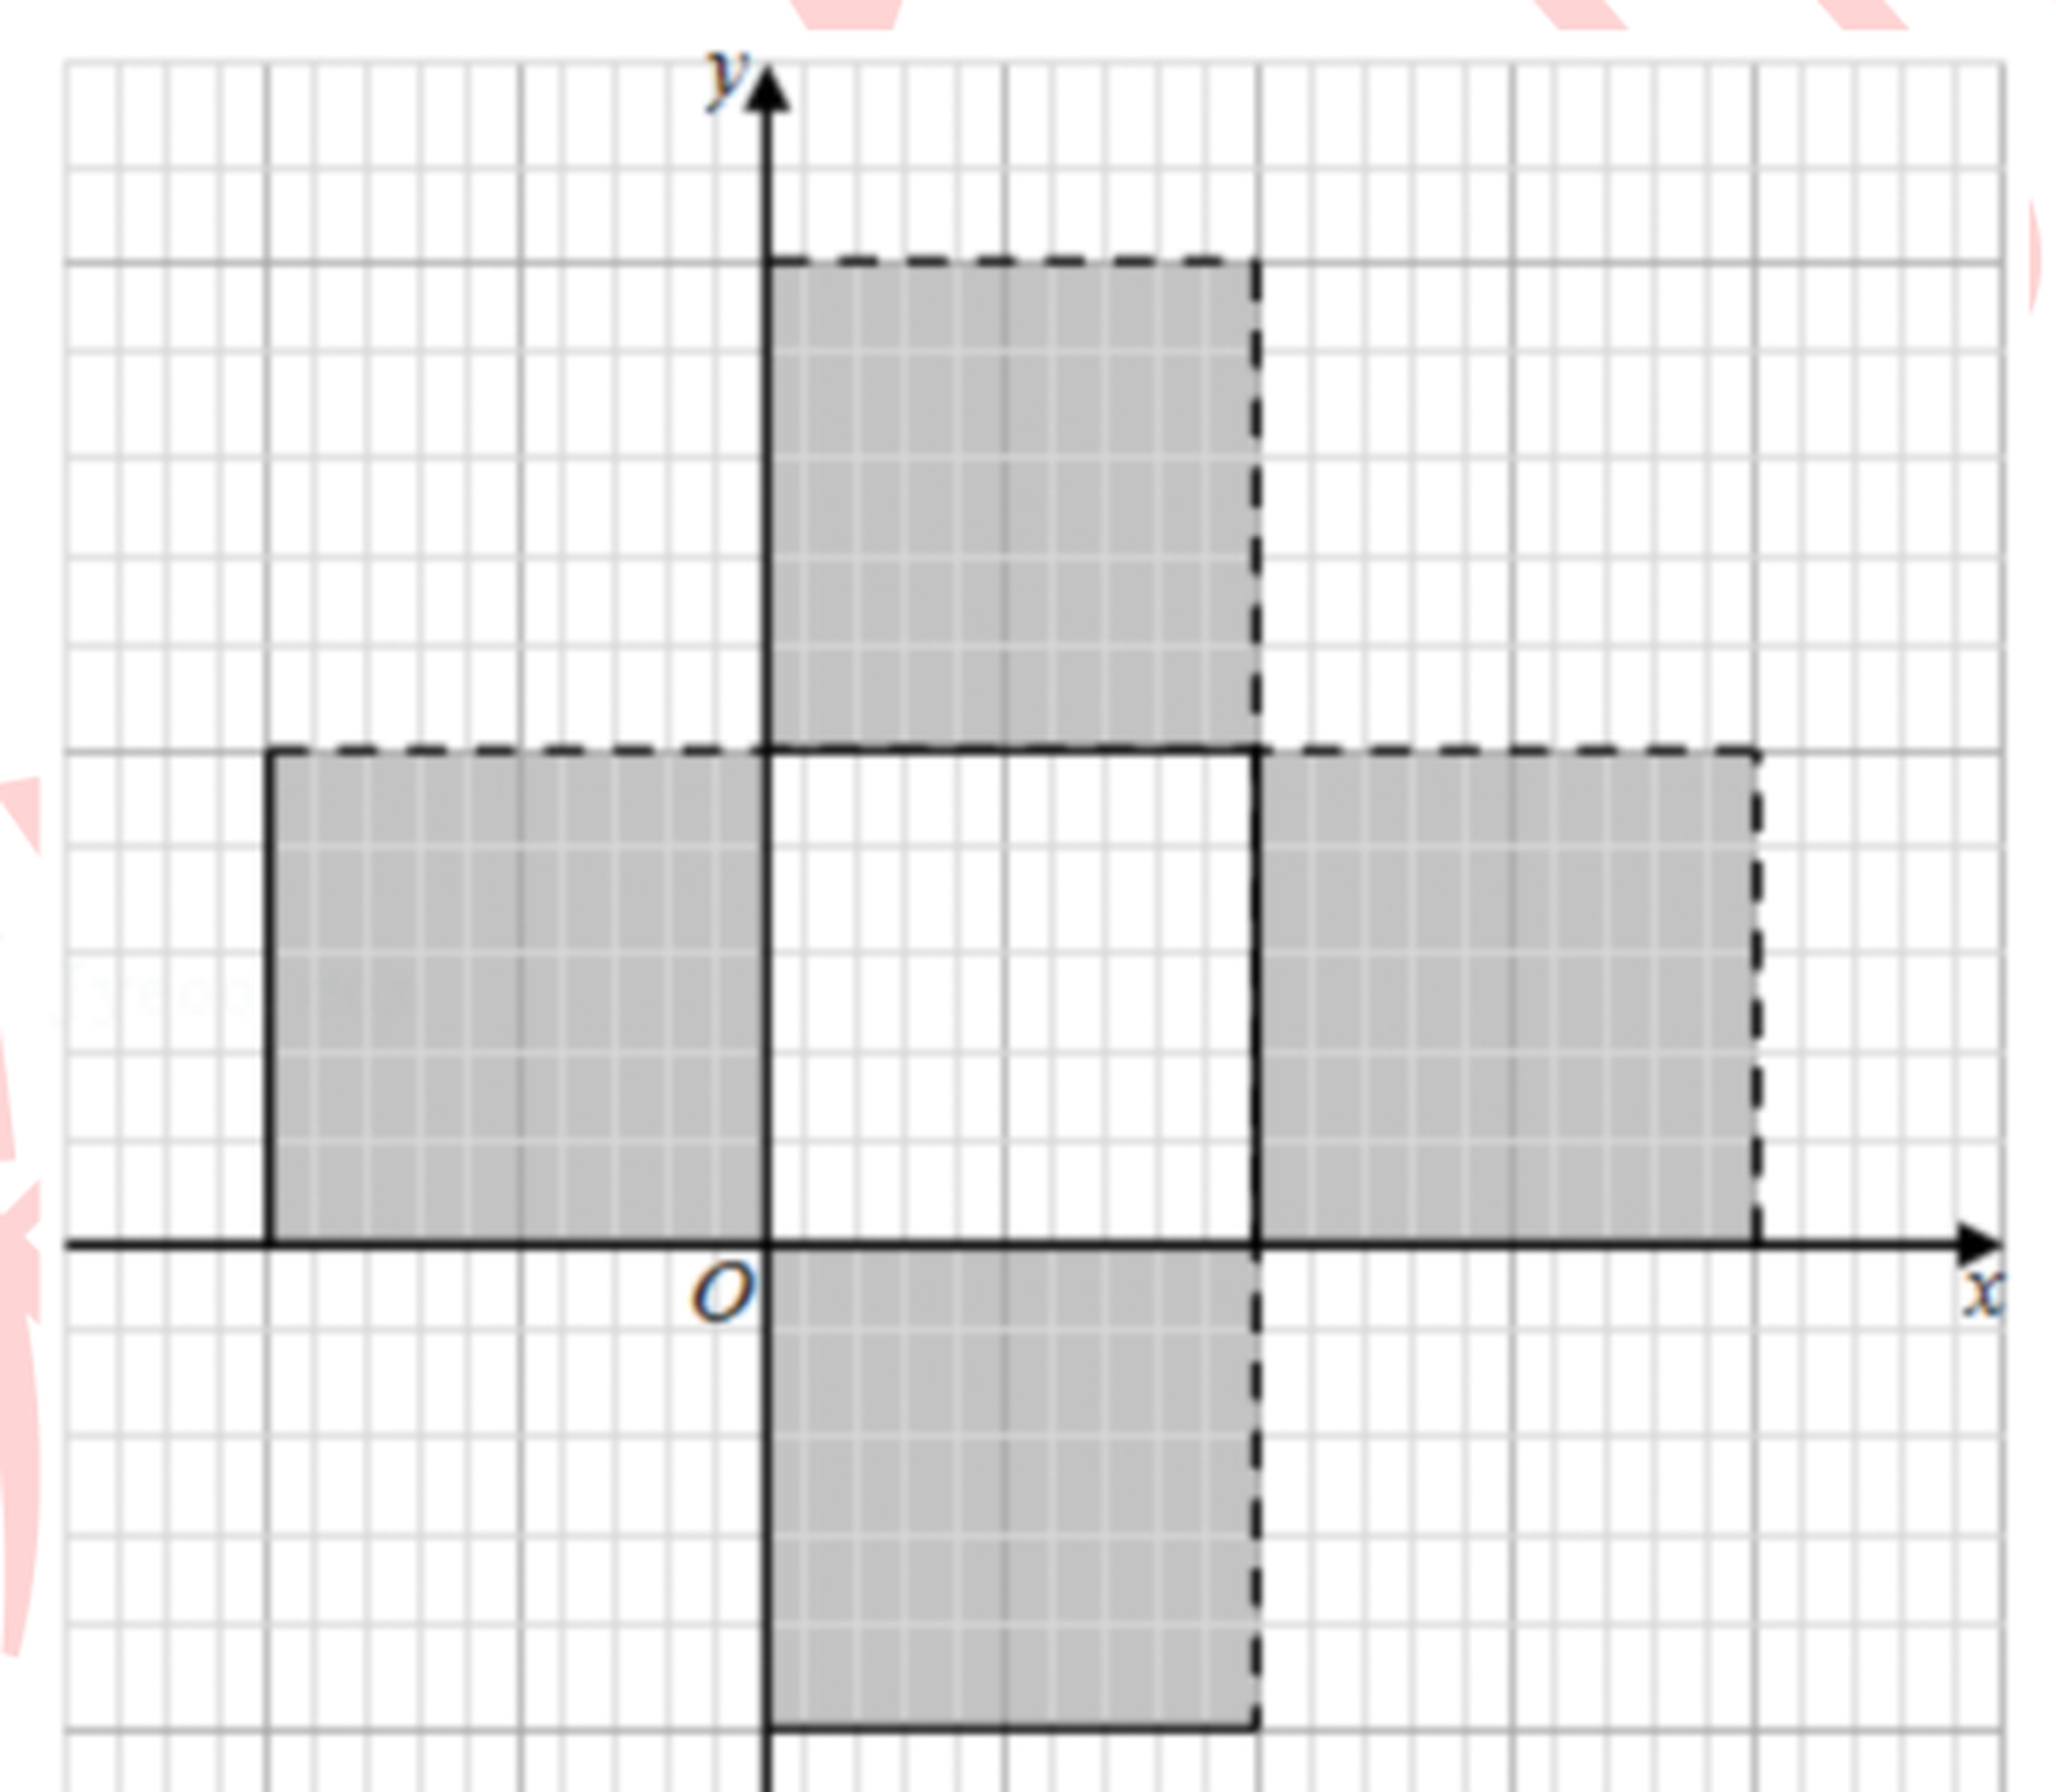
\includegraphics[width=0.38\textwidth]{figures/plane_grid_4squares_h39.png}
\end{center}
\step{总面积为 $1\times4=4$.}
\solend

\fi

\item 关于 $x$ 的不等式 $ax^2+bx+c>0$ 的解集为 $\{x\mid x<\beta\text{ 或 }x>\gamma\}(0<\beta<\gamma)$，
则不等式 $a(x^2+1)+b(x-1)+c>2ax$ 的解集为 \blankline[4.4em].

\ans{$(-\infty,\beta+1)\cup(\gamma+1,+\infty)$}

\ifanswer
\solbegin
\step{由题意得 $\beta$、$\gamma$ 为方程 $ax^2+bx+c=0$ 的两根且 $a>0$，}
\step{则 $\beta+\gamma=-\dfrac ba$，$\beta\gamma=\dfrac ca$，故 $b=-a(\beta+\gamma)$，$c=\beta\gamma a$，}
\step{则不等式可化为 $a(x^2+1)-a(\beta+\gamma)(x-1)+\beta\gamma a>2ax$，}
\step{因为 $a>0$，所以 $x^2+1-(\beta+\gamma)(x-1)+\beta\gamma>2x$，}
\step{即 $x^2-(\beta+\gamma+2)x+(\beta+\gamma+\beta\gamma+1)>0$，所以 $(x-\beta-1)(x-\gamma-1)>0$，}
\step{解得 $x<\beta+1$ 或 $x>\gamma+1$，所以不等式解集为 $(-\infty,\beta+1)\cup(\gamma+1,+\infty)$.}
\solend

\fi

\end{enumerate}

\bigsec{二、选择题}

\begin{enumerate}
\setcounter{enumi}{12}

\item 设 $a<b<0$，则下列不等式中不成立的是\mbox{（\quad）}

\keepwithprev
A. $\dfrac1a>\dfrac1b$\qquad B. $\dfrac{1}{a-b}>\dfrac1a$\qquad C. $|a|>-b$\qquad D. $\sqrt{-a}>\sqrt{-b}$

\ans{$B$}

\ifanswer
\solbegin
\step{令 $a=-2$，$b=-1$，}
\step{A、$-\dfrac12>-1$，正确；B、$-1<-\dfrac12$，故 B 错误；C、$2>1$，正确；}
\step{D、$\sqrt2>1$，正确；故选 B.}
\solend

\fi

\item 设实数集 $\R$ 为全集，集合 $P=\{x\mid f(x)=0\}$，$Q=\{x\mid g(x)=0\}$，$H=\{x\mid h(x)=0\}$，
则方程 $\dfrac{f^2(x)+g^2(x)}{h(x)}=0$ 的解集是\mbox{（\quad）}

\keepwithprev
A. $P\cap Q\cap\overline{H}$\qquad B. $P\cap Q$\qquad C. $P\cap Q\cap H$\qquad D. $P\cap Q\cup H$

\ans{$A$}

\ifanswer
\solbegin
\step{方程 $\dfrac{f^2(x)+g^2(x)}{h(x)}=0$ 等价于 $\begin{cases}f(x)=0\\ g(x)=0\\ h(x)\neq0\end{cases}$，}
\step{又因为 $P=\{x\mid f(x)=0\}$，$Q=\{x\mid g(x)=0\}$，$H=\{x\mid h(x)=0\}$，}
\step{所以方程 $\dfrac{f^2(x)+g^2(x)}{h(x)}=0$ 的解集是 $P\cap Q\cap\overline{H}$，故选 A.}
\solend

\fi

\item 设全集 $U$，在下列条件中，是 $B\sub A$ 的充要条件的有\mbox{（\quad）}

\keepwithprev
% 注：原卷此行 ② 与 ③ 之间**漏排分隔号**（①、③ 后都有「；」，② 后没有）；
%     本稿照录未补，见文件头「原卷笔误/存疑」⑩。
①$A\cup B=A$；\qquad ②$\overline{A}\cap B=\varnothing$\qquad ③$\overline{A}\sub\overline{B}$；\qquad ④$A\cup\overline{B}=U$

\keepwithprev
A. $1$ 个\qquad B. $2$ 个\qquad C. $3$ 个\qquad D. $4$ 个

\ans{$D$}

\item 已知集合 $M=\{x\mid x\in\N,0<x\leqslant15\}$，$A_1$、$A_2$、$A_3$ 满足：①$A_1\cup A_2\cup A_3=M$；
②每个集合都恰有 $5$ 个元素. 集合 $A_i(i=1,2,3)$ 中最大元素与最小元素之和称为 $A_i$ 的特征数，
记为 $X_i(i=1,2,3)$，则 $X_1+X_2+X_3$ 的值不可能为\mbox{（\quad）}

\keepwithprev
A. $37$\qquad B. $39$\qquad C. $48$\qquad D. $57$

\ans{$A$}

\ifanswer
\solbegin
\step{因为集合 $M=\{x\mid x\in\N,0<x\leqslant15\}=\{1,2,3,\cdots,15\}$，}
\step{又因为集合 $A_1$、$A_2$、$A_3$ 中，每个集合恰有 $5$ 个元素，}
\step{且 $A_1\cup A_2\cup A_3=M$ 有 $15$ 个元素，所以集合 $A_1$、$A_2$、$A_3$ 中没有重复元素，}
\step{因为 $1$ 是集合 $M$ 中数值最小的元素，$15$ 是集合 $M$ 中数值最大的元素，}
\step{所以在 $A_i$ 的特征数构成中，必有 $1$ 和 $15$，不妨设 $1\in A_1$，$15\in A_1$，}
% 注：原卷本行（与下面「最小」那句）在「集合」后的角标是**数字 $1$**（同句 $X_1$ 的角标同形），
%     而非上一行「$A_i$ 的特征数构成」里的斜体 $A_i$——原卷两种下标并存，本稿照录、不归一，
%     见文件头「原卷笔误/存疑」⑬。
\step{要使 $X_1+X_2+X_3$ 最大，则应该在集合 $A_1$ 中首先放置数值较小的元素，}
\step{即 $A_1=\{1,2,3,4,15\}$，所以 $5$ 与 $14$ 是剩下元素中数值最小或最大的元素，}
\step{同理，不妨设 $5\in A_2$，$14\in A_2$，接着在 $A_2$ 中再次放置数值较小的元素，}
\step{即 $A_2=\{5,6,7,8,14\}$，则 $A_3=\{9,10,11,12,13\}$，}
\step{此时 $X_1+X_2+X_3$ 有最大值为 $1+15+5+14+9+13=57$，}
\step{即 $X_1+X_2+X_3\leqslant57$；}
% 注：同上一处——原卷此行角标是**数字 $1$**（$A_1$），本稿照录，未与「$A_i$」归一。
\step{要使 $X_1+X_2+X_3$ 最小，则在集合 $A_1$ 中首先放置数值较大的元素，}
\step{即 $A_1=\{1,12,13,14,15\}$，所以 $2$ 与 $11$ 是剩下元素中数值最小或最大的元素，}
\step{同理，不妨设 $2\in A_2$，$11\in A_2$，接着在 $A_2$ 中再次放置数值较大的元素，}
\step{即 $A_2=\{2,8,9,10,11\}$，则 $A_3=\{3,4,5,6,7\}$，}
\step{此时 $X_1+X_2+X_3$ 有最小值为 $1+15+2+11+3+7=39$，}
\step{即 $X_1+X_2+X_3\geqslant39$，}
\step{综上，$39\leqslant X_1+X_2+X_3\leqslant57$，故选 A.}
\solend

\fi

\end{enumerate}

\bigsec{三、解答题}

\begin{enumerate}
\setcounter{enumi}{16}

% 注：原卷首句「由数 $y=-x^2+ax-1=-x+3$」中的「由数」显系「由」或「由函数」之误；末段
%     的两处分类讨论与结论自相矛盾（详见文件头「笔误/存疑」④）。本稿一律照录，未改。
\item 命题 $p$：函数 $y=-x^2+ax-1$ 与 $y=-x+3$ 图象交点的横坐标均为负值，
命题 $q$：关于 $x$ 的方程 $2(1-x)a+(x^2-10x-3)=0$ 的两个根，一个大于 $3$，另一个小于 $3$；
若命题 $p$ 和命题 $q$ 中有且仅有一个是真命题，求 $a$ 的取值范围.

\ans{$\R$}

\ifanswer
\solbegin
\step{由数 $y=-x^2+ax-1=-x+3$ 得 $x^2-(a+1)x+4=0$，}
\step{若横坐标均为负值，则满足 $\begin{cases}\Delta=(a+1)^2-16\geqslant0\\ x_1x_2=4>0\\ x_1+x_2=a+1<0\end{cases}$
得 $\begin{cases}a\geqslant3\text{ 或 }a\leqslant-5\\ a<-1\end{cases}$，得 $a\leqslant-5$，}
\step{即 $p:a\leqslant-5$，}
\step{若方程 $2(1-x)a+(x^2-10x-3)=0$ 的两个根，一个大于 $3$，另一个小于 $3$；}
\step{设 $f(x)=2(1-x)a+(x^2-10x-3)$，则 $f(3)<0$，即 $-4a-24<0$，}
\step{得 $a>-6$，即 $q:a>-6$，}
\step{因为命题 $p$ 和命题 $q$ 中有且仅有一个是真命题，}
\step{若 $p$ 真 $q$ 假，则 $\begin{cases}a\leqslant-5\\ a>-6\end{cases}$，得 $a\in\R$，}
\step{若 $p$ 假 $q$ 真，则 $\begin{cases}a>-5\\ a\leqslant-6\end{cases}$，此时 $a$ 无解，}
\step{综上，实数 $a$ 的取值范围是 $\R$.}
\solend

\fi

\ansspace[8]

\item 设全集是实数集 $\R$，$A=\left\{x\mid\dfrac{1-2x}{x-3}\geqslant0\right\}$，$B=\{x\mid x^2+a\leqslant0\}$.

\begin{enumerate}[label=(\arabic*)]

\item 当 $a=-4$ 时，求 $A\cup B$；

\item 若 $\overline{A}\cap B=B$，求实数 $a$ 的取值范围.

\end{enumerate}

\ans{（1）$\{x\mid-2\leqslant x<3\}$；（2）$\left(-\dfrac14,+\infty\right)$}

\ifanswer
\solbegin
\stepm{(1)}{$A=\left\{x\mid\dfrac{1-2x}{x-3}\geqslant0\right\}=\left\{x\mid\dfrac12\leqslant x<3\right\}$，$B=\{x\mid x^2+a\leqslant0\}$.}
\step{当 $a=-4$ 时，$B=\{x\mid-2\leqslant x\leqslant2\}$，所以 $A\cup B=\{x\mid-2\leqslant x<3\}$.}
\stepm{(2)}{$\overline{A}=\left\{x\mid x\geqslant3\text{ 或 }x<\dfrac12\right\}$，$B=\{x\mid x^2+a\leqslant0\}$.}
\step{由 $\overline{A}\cap B=B$，得 $B\sub\overline{A}$，}
\step{则当 $a>0$ 时，$B=\varnothing$，满足 $B\sub\overline{A}$，则 $a>0$ 成立，}
\step{则当 $a=0$ 时，$B=\{0\}$，满足 $B\sub\overline{A}$，则 $a=0$ 成立，}
\step{当 $a<0$ 时，$B=\{x\mid-\sqrt{-a}\leqslant x<\sqrt{-a}\}$，}
\step{得 $\sqrt{-a}<\dfrac12$，即 $-\dfrac14<a<0$，}
\step{综上，实数 $a$ 的取值范围是 $\left(-\dfrac14,+\infty\right)$.}
\solend

\fi

\ansspace[6]

\item 设集合 $A=\{x\mid ax^2+2x+1=0,a\in\R\}$.

\begin{enumerate}[label=(\arabic*)]

\item 当 $A$ 中元素个数为 $1$ 时，求：$a$ 和 $A$；

\item 当 $A$ 中元素个数至少为 $1$ 时，求：$a$ 的取值范围；

\item 求：$A$ 中各元素之和.

\end{enumerate}

\ans{（1）$a=0$ 时 $A=\left\{-\dfrac12\right\}$，$a=1$ 时 $A=\{-1\}$；（2）$(-\infty,1]$；
（3）$a=0$ 时和为 $-\dfrac12$，$a<1$ 且 $a\neq0$ 时和为 $-\dfrac2a$，$a=1$ 时和为 $-1$，$a>1$ 时 $A$ 中无元素}

\ifanswer
\solbegin
\stepm{(1)}{集合 $A=\{x\mid ax^2+2x+1=0,a\in\R\}$，$A$ 中元素个数为 $1$，}
\step{所以 $a=0$ 或 $\begin{cases}a\neq0\\ \Delta=4-4a=0\end{cases}$，解得 $a=0$，$A=\left\{-\dfrac12\right\}$ 或 $a=1$，$A=\{-1\}$.}
\stepm{(2)}{当 $A$ 中元素个数至少为 $1$ 时，$a=0$ 或 $\begin{cases}a\neq0\\ \Delta=4-4a\geqslant0\end{cases}$，解得 $a\leqslant1$，}
\step{所以 $a$ 的取值范围是 $(-\infty,1]$.}
\stepm{(3)}{当 $a=0$ 时，$A$ 中元素之和为 $-\dfrac12$；}
\step{当 $a<1$ 且 $a\neq0$ 时，$A$ 中元素之和为 $-\dfrac2a$；}
\step{当 $a=1$ 时，$A$ 中元素之和为 $-1$；}
\step{当 $a>1$ 时，$A$ 中无元素.}
\solend

\fi

\ansspace[8]

\item 设 $k$ 是正整数，集合 $A$ 至少有两个元素，且 $A\sub\N^*$. 如果对于 $A$ 中的任意两个不同的
元素 $x$、$y$，都有 $|x-y|\neq k$，则称 $A$ 具有性质 $P(k)$.

\begin{enumerate}[label=(\arabic*)]

\item 试判断集合 $B=\{1,2,3,4\}$ 和 $C=\{1,4,7,10\}$ 是否具有性质 $P(2)$？并说明理由；

\item 若集合 $A=\{a_1,a_2,\cdots,a_{12}\}\sub\{1,2,\cdots,20\}$，求证：$A$ 不可能具有性质 $P(3)$；

\item 若集合 $A\sub\{1,2,\cdots,2023\}$，且同时具有性质 $P(4)$ 和 $P(7)$，求集合 $A$ 中元素个数的
最大值.

\end{enumerate}

\ans{（1）$B$ 不具有性质 $P(2)$，$C$ 具有性质 $P(2)$；（2）见解析；（3）$920$}

\ifanswer
\solbegin
\stepm{(1)}{因为 $B=\{1,2,3,4\}$，}
\step{又 $1\in\N^*$，$2\in\N^*$，$3\in\N^*$，$4\in\N^*$，但 $|4-2|=2$，}
\step{所以集合 $B$ 不具有性质 $P(2)$，}
\step{因为 $C=\{1,4,7,10\}$，}
\step{又 $1\in\N^*$，$4\in\N^*$，$7\in\N^*$，$10\in\N^*$，}
\step{但 $|4-1|=3$，$|7-1|=6$，$|10-1|=9$，$|7-4|=3$，$|10-4|=6$，$|10-7|=3$，}
\step{所以集合 $C$ 具有性质 $P(2)$，}
\stepm{(2)}{将集合 $\{1,2,\cdots,20\}$ 中的元素分为如下 $11$ 个集合，}
% 注：原卷本行 $\{8,11\}$ 与 $\{9,12\}$ 之间的分隔号误用**句号**「.」（同行其余处皆逗号），
%     本稿照录、未改，见文件头「原卷笔误/存疑」⑪。
\step{$\{1,4\}$，$\{2,5\}$，$\{3,6\}$，$\{7,10\}$，$\{8,11\}$.$\{9,12\}$，$\{13,16\}$，$\{14,17\}$，$\{15,18\}$，}
\step{$\{19\}$，$\{20\}$，}
\step{所以从集合 $\{1,2,\cdots,20\}$ 中取 $12$ 个元素，则前 $9$ 个集合至少要选 $10$ 个元素，}
\step{所以必有 $2$ 个元素取自前 $9$ 个集合中的同一集合，即存在两个元素其差为 $3$，}
\step{所以 $A$ 不可能具有性质 $P(3)$；}
\stepm{(3)}{先说明连续 $11$ 项中集合 $A$ 中最多选取 $5$ 项，}
\step{以 $1,2,3,\cdots,11$ 为例.}
\step{构造抽屉 $\{1,8\}$，$\{2,9\}$，$\{3,10\}$，$\{4,11\}$，$\{5\}$，$\{6\}$，$\{7\}$.}
\step{①$5$、$6$、$7$ 同时选，因为具有性质 $P(4)$ 和 $P(7)$，}
\step{所以选 $5$ 则不选 $1$、$9$；选 $6$ 则不选 $2$、$10$；选 $7$ 则不选 $3$、$11$；}
% 注：原卷此步推理不严——「只剩 $4$、$8$」但两数相差 $4$、不能同选，该情形实际最多只能取 $4$ 个；
%     末句「不超过 $5$ 个」的结论仍成立。本稿照录，见文件头「原卷笔误/存疑」⑫。
\step{则只剩 $4$、$8$；故 $1,2,3,\cdots,11$ 中属于集合 $A$ 的元素个数不超过 $5$ 个.}
\step{②$5$、$6$、$7$ 选 $2$ 个，}
\step{若只选 $5$、$6$，则 $1$、$2$、$9$、$10$、$7$ 不可选，又 $\{4,11\}$ 只能选一个元素，}
\step{$3$、$8$ 可以选，故 $1,2,3,\cdots,11$ 中属于集合 $A$ 的元素个数不超过 $5$ 个.}
\step{若选 $5$、$7$，则只能从 $2$、$4$、$8$、$10$ 中选，但 $4$、$8$ 不能同时选，}
\step{故 $1,2,3,\cdots,11$ 中属于集合 $A$ 的元素个数不超过 $5$ 个.}
\step{若选 $6$、$7$，则 $2$、$3$、$10$、$11$、$5$ 不可选，又 $\{1,8\}$ 只能选一个元素，}
\step{$4$、$9$ 可以选，故 $1,2,3,\cdots,11$ 中属于集合 $A$ 的元素个数不超过 $5$ 个.}
\step{③$5$、$6$、$7$ 中只选 $1$ 个，}
\step{又四个集合 $\{1,8\}$，$\{2,9\}$，$\{3,10\}$，$\{4,11\}$ 每个集合至多选 $1$ 个元素，}
\step{故 $1,2,3,\cdots,11$ 中属于集合 $A$ 的元素个数不超过 $5$ 个.}
\step{由上述①②③得，连续 $11$ 项自然数中属于集合 $A$ 的元素至多只有 $5$ 个，}
\step{如取 $1$、$4$、$6$、$7$、$9$.}
\step{因为 $2023=183\times11+10$，则把每 $11$ 个连续自然数分组，}
\step{前 $183$ 组每组至多选取 $5$ 项；}
\step{从 $2014$ 开始，最后 $10$ 个数至多选取 $5$ 项，}
\step{故集合 $A$ 的元素最多有 $184\times5=920$ 个.}
\step{给出如下选取方法：从 $1,2,3,\cdots,11$ 中选取 $1$、$4$、$6$、$7$、$9$；}
\step{然后在这 $5$ 个数的基础上每次累加 $11$，构造 $183$ 次.}
\step{此时集合 $A$ 的元素为 $1$，$4$，$6$，$7$，$9$；$12$，$15$，$17$，$18$，$20$；$23$，$26$，$28$，$29$，$31$；
$\cdots$；$2014$，$2017$，$2019$，$2020$，$2022$，共 $920$ 个元素.}
\step{经检验得该集合符合要求，故集合 $A$ 的元素最多有 $920$ 个.}
\solend

\fi

\ansspace[10]

\end{enumerate}

\bigsec{附加题}

\begin{enumerate}
\setcounter{enumi}{20}

\item 若规定集合 $M=\{a_1,a_2,\cdots,a_n\}$（$n\in\N^*$）的子集 $\{a_{i_1},a_{i_2},\cdots,a_{i_m}\}$（$m\in\N^*$）
为 $M$ 的第 $k$ 个子集，其中 $k=2^{i_1-1}+2^{i_2-1}+\cdots+2^{i_m-1}$，则 $M$ 的第 $25$ 个子集是 \blankline[4.4em].

\ans{$\{a_1,a_4,a_5\}$}

\ifanswer
\solbegin
\step{由题意得 $M$ 的第 $k$ 个子集，且 $k=2^{i_1-1}+2^{i_2-1}+\cdots+2^{i_m-1}$，}
\step{又 $25=2^0+2^3+2^4=2^{1-1}+2^{4-1}+2^{5-1}$，所以 $M$ 的第 $25$ 个子集是 $\{a_1,a_4,a_5\}$.}
\solend

\fi

% 注：原卷在 $x=1$、$y=2$、$z=3$ 时把 $B=\{x,y\}$ 印作 $\{1,3\}$（应为 $\{1,2\}$），
%     照录未改，见文件头「笔误/存疑」⑥。
\item 用 $|S|$ 表示集合 $S$ 中的元素的个数，设 $A$、$B$、$C$ 为集合，称 $(A,B,C)$ 为有序三元组.
如果集合 $A$、$B$、$C$ 满足 $|A\cap B|=|B\cap C|=|C\cap A|=1$，且 $A\cap B\cap C=\varnothing$，
则称有序三元组 $(A,B,C)$ 为最小相交. 由集合 $\{1,2,3\}$ 的子集构成的所有有序三元组中，
最小相交的有序三元组的个数为 \blankline[4.4em].

\ans{$6$}

\ifanswer
\solbegin
\step{因为 $|A\cap B|=|B\cap C|=|C\cap A|=1$，}
\step{所以设 $A\cap B=\{x\}$，$B\cap C=\{y\}$，$C\cap A=\{z\}$，}
% 图在【解析】内（仅答案版出），取原卷截图（10.png，2560×3620）右栏，4× LANCZOS 放大。
\begin{center}
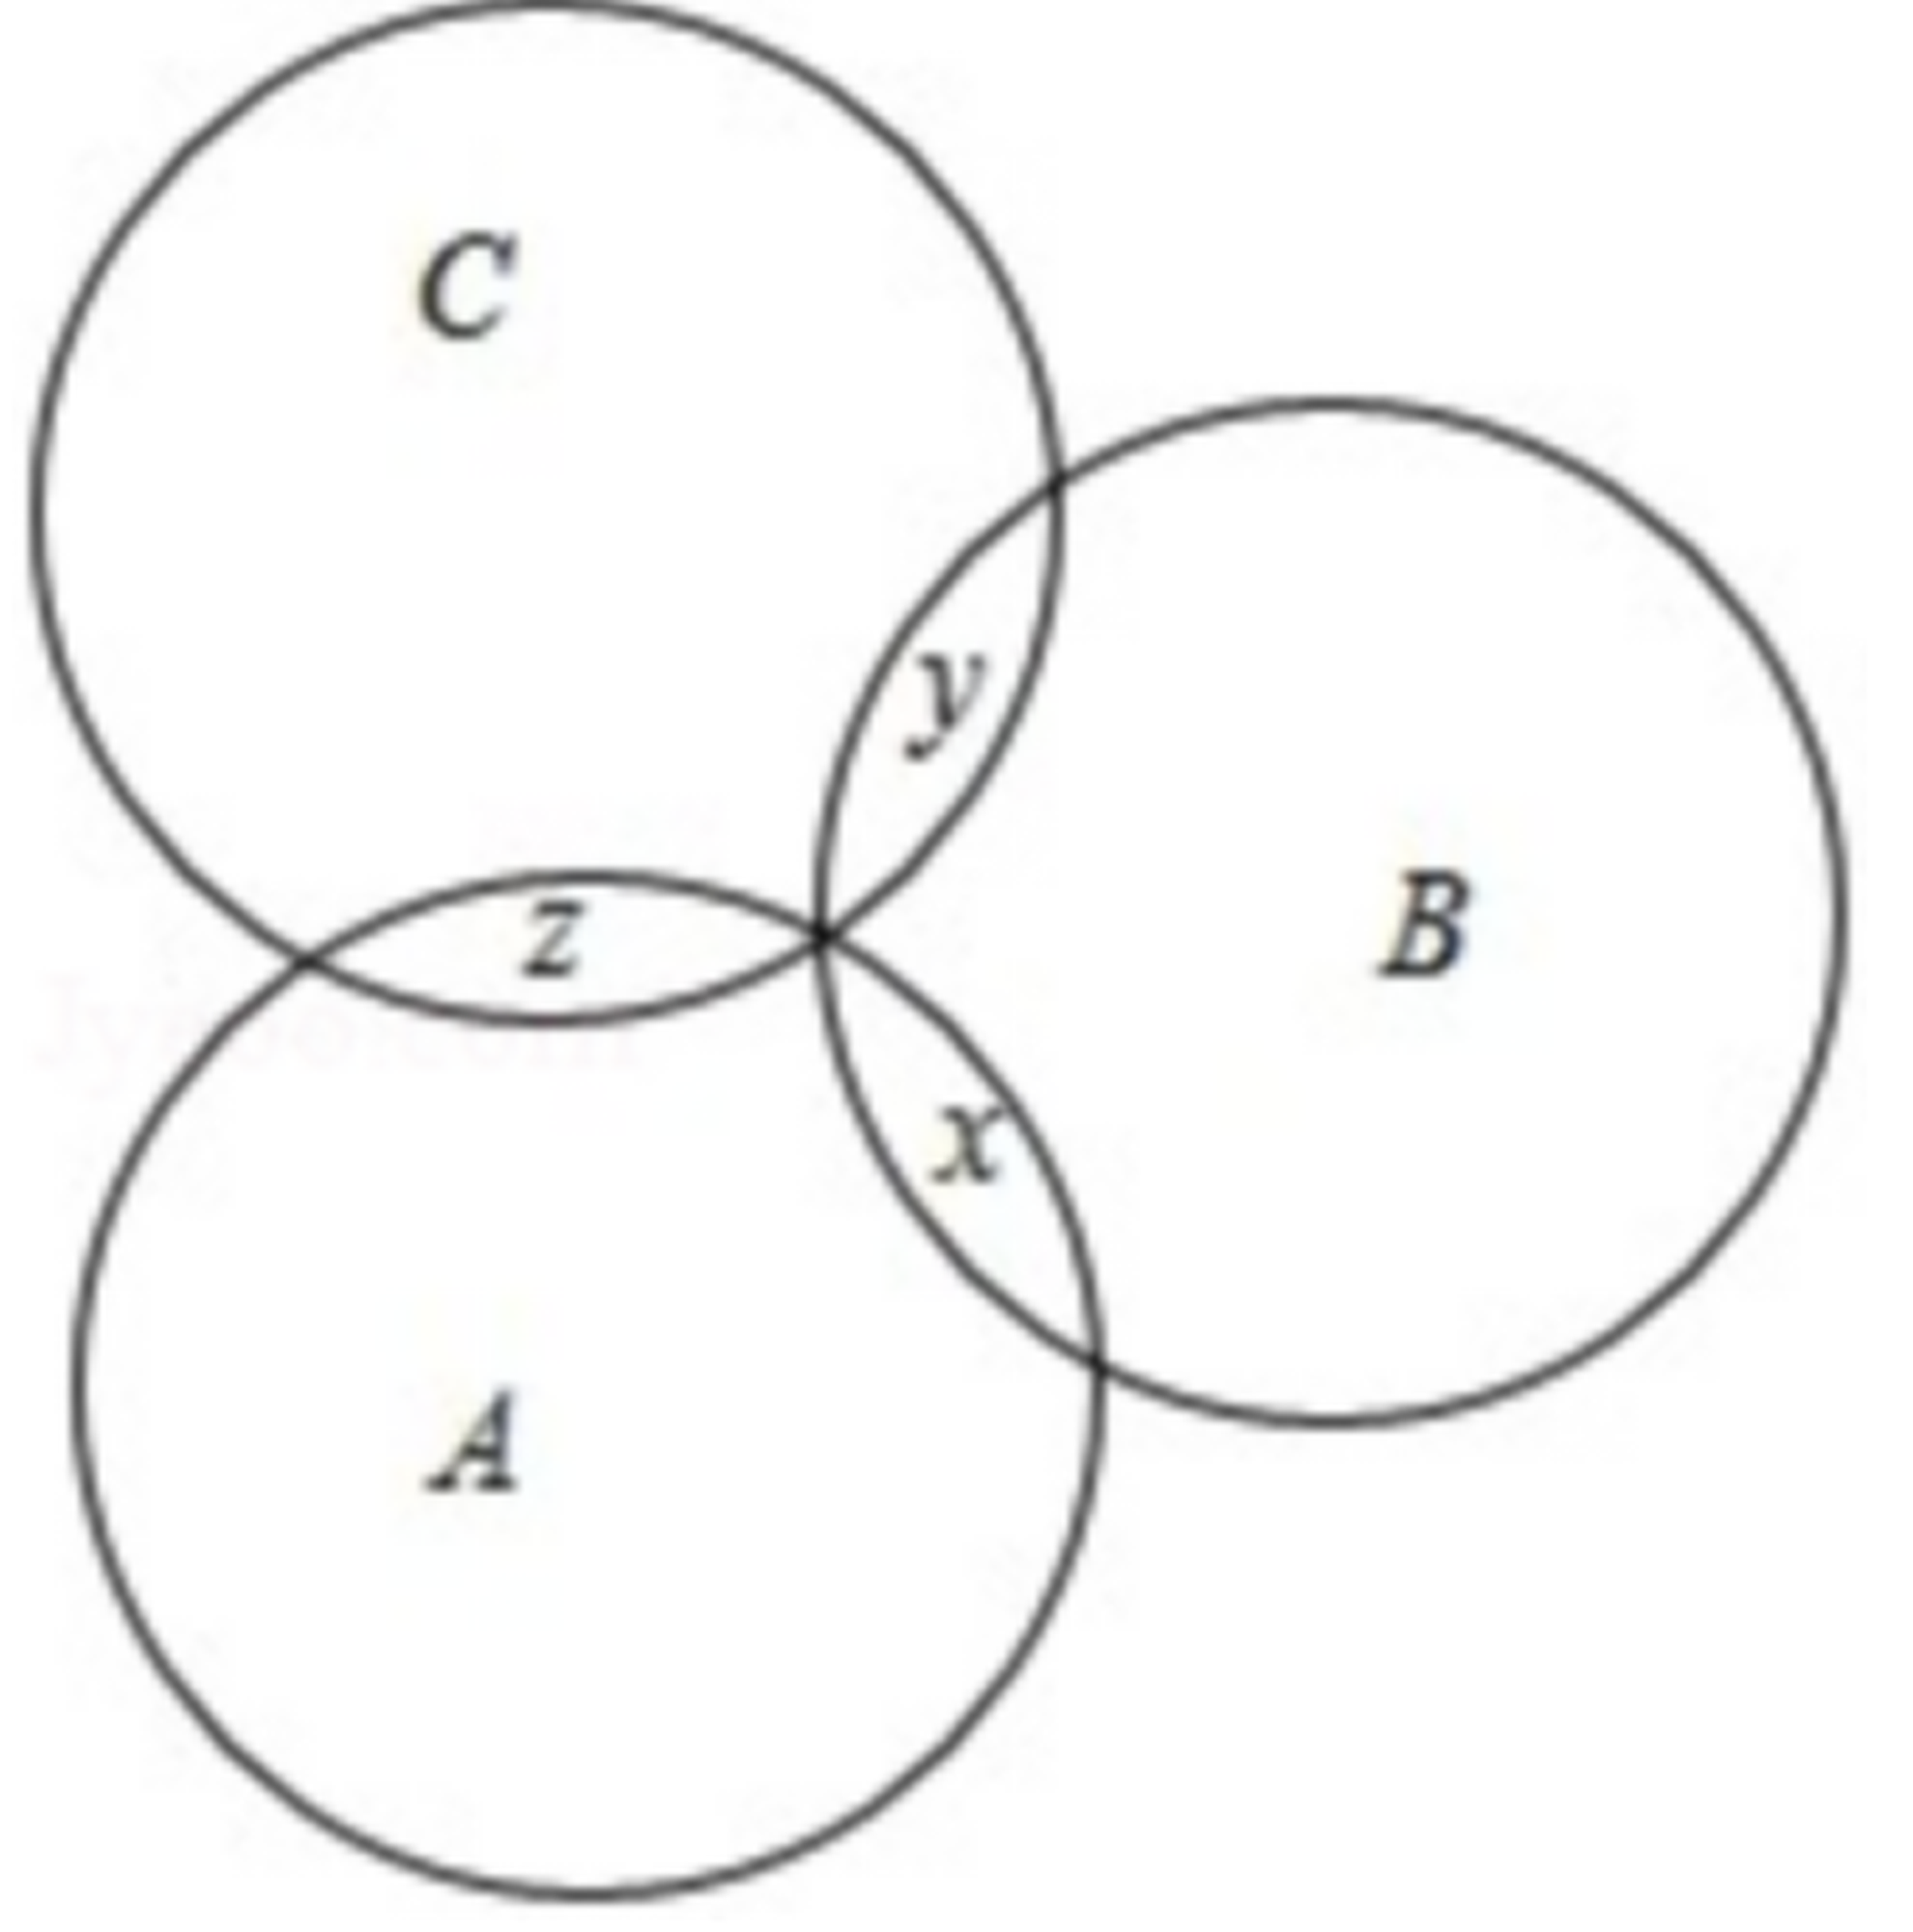
\includegraphics[width=0.30\textwidth]{figures/venn_ABC_x_y_z_h39.png}
\end{center}
\step{因为 $|A\cap B|=|B\cap C|=|C\cap A|=1$，且 $x$、$y$、$z\in\{1,2,3\}$，}
\step{所以集合 $A=\{x,z\}$，$B=\{x,y\}$，$C=\{z,y\}$，}
\step{若 $x=1$，$y=2$，$z=3$，则 $A=\{1,3\}$，$B=\{1,3\}$，$C=\{2,3\}$，}
\step{将 $1$，$2$，$3$ 进行全排列，有 $P_3^3=3\times2=6$ 个.}
\solend

\fi

\item 已知集合 $T=\{1,2,\cdots,2025\}$，对于 $T$ 的每一个非空子集的所有元素，计算它们乘积的倒数，
则所有这样倒数的和为 \blankline[4.4em].

\ans{$2025$}

\ifanswer
\solbegin
\step{集合 $T=\{1,2,\cdots,2025\}$ 的非空子集的个数为 $2^{2025}-1$，}
\step{这些子集中，每个元素的乘积分别为}
\step{$1,2,3,\cdots,2025,1\times2,1\times3,\cdots,1\times2025,\cdots,1\times2\times3\times\cdots\times2025$，}
\step{每项都可以看作是从 $1,2,3,\cdots,2025$ 中选择若干项的乘积，}
\step{$1+\dfrac12+\cdots+\dfrac{1}{2025}+\dfrac{1}{1\times2}+\dfrac{1}{1\times3}+\cdots+\dfrac{1}{2024\times2025}
+\cdots+\dfrac{1}{1\times2\times\cdots\times2025}$}
\step{$=(1+1)\left(1+\dfrac12\right)\cdots\left(1+\dfrac{1}{2025}\right)-1
=2\times\dfrac32\times\dfrac43\times\cdots\times\dfrac{2026}{2025}-1=2025$.}
\solend

\fi

% 第 24 题是压轴题，题干较长；试卷版在它之前量一次页高，尽量不与前文分家（照全稿成例）。
\ansneed{5cm}
% 注：原卷【解析】①③ 两步把 $f(x)$ 印作 $f[x[x]]$，显系笔误，照录未改，见文件头「笔误/存疑」⑦。
\item 若 $X$ 是一个集合，$T$ 是一个以 $X$ 的某些子集为元素的集合，且满足：①$X$ 属于 $T$，
$\varnothing$ 属于 $T$；②$T$ 中任意多个元素的并集属于 $T$；③$T$ 中任意多个元素的交集属于 $T$.
则称 $T$ 是集合 $X$ 上的一个拓扑. 已知函数 $f(x)=[x[x]]$，其中 $[x]$ 表示不大于 $x$ 的最大整数，
当 $x\in(0,n]$，$n\in\N^*$ 时，函数 $f(x)$ 值域为集合 $A_n$，则集合 $A_2$ 上的含有 $4$ 个元素的
拓扑 $T$ 的个数为 \blankline[4.4em].

\ans{$9$}

\ifanswer
\solbegin
\step{由题意，$n=2$，故 $0<x\leqslant2$，}
\step{①当 $0<x<1$ 时，则 $[x]=0$，所以 $f[x[x]]=0$，}
\step{②当 $x=1$ 时，$[x]=1$ 显然 $f(1)=1$，}
\step{③当 $1<x<2$ 时，$[x]=1$，所以 $f[x[x]]=[x]=1$，}
\step{④当 $x=2$ 时，$f(2)=4$，}
\step{所以 $A_2=\{0,1,4\}$，}
\step{因为 $T$ 中含有 $4$ 个元素，其中两个元素 $\varnothing$ 和 $A_2$，}
\step{$A_2=\{0,1,4\}$. 其它两个元素为 $A$、$B$，则
$\begin{cases}A\neq\varnothing\\ A\neq A_2\\ B\neq\varnothing\\ B\neq A_2\\ A\neq B\end{cases}$，}
\step{由对称性，不妨设 $1\leqslant|A|\leqslant|B|\leqslant2$，其中 $|A|$、$|B|$ 表示集合 $A$ 中元素的个数，}
\step{因为 $\begin{cases}A\cap B\in T\\ A\cup B\in T\end{cases}$，又 $|A|\leqslant|B|$，所以 $A\cap B=\varnothing$ 或 $A$，}
\step{若 $A\cap B=\varnothing$，则 $A\cup B$ 只能等于 $A_2$，}
\step{（若 $A\cup B=B$，则 $A\sub B$，则 $A\cap B=A=\varnothing$，矛盾）}
\step{则必有 $\begin{cases}|A|=1\\ |B|=2\end{cases}$，所以 $(A,B)$ 的个数 $\Leftrightarrow$ $A$ 的个数 $=3$ 种，}
\step{即 $\begin{cases}A=\{0\}\\ B=\{1,4\}\end{cases}$ 或 $\begin{cases}A=\{1\}\\ B=\{0,4\}\end{cases}$
或 $\begin{cases}A=\{4\}\\ B=\{0,1\}\end{cases}$；}
\step{若 $A\cap B=A\Leftrightarrow A\sub B$ 此时满足 $A\cup B=B$，}
\step{因为 $A\neq B$ 且 $1\leqslant|A|$ 且 $|B|\leqslant2$，所以 $\begin{cases}|A|=1\\ |B|=2\end{cases}$，}
\step{所以 $B$ 的选择共有 $C_3^2=3$ 种，则 $A$ 的个数有 $C_2^1$ 种，}
\step{所以 $(A,B)$ 的个数 $=2\times3=6$ 种.}
% 这六组「$A$／$B$」按原卷排作两行（前五个一行、第六个另起一行）；因五组并排时
% amsmath 的 cases 会为每组的第二列各留一枚 \quad，本行改排 \left\{\begin{matrix}…\end{matrix}\right.
% 以省下这枚 \quad（照 README「说明」记的高一07 成例），字形与 cases 相同。
\step{（这 $6$ 种是 $\left\{\begin{matrix}A=\{0\}\\ B=\{0,1\}\end{matrix}\right.$、
$\left\{\begin{matrix}A=\{1\}\\ B=\{0,1\}\end{matrix}\right.$、
$\left\{\begin{matrix}A=\{0\}\\ B=\{0,4\}\end{matrix}\right.$、
$\left\{\begin{matrix}A=\{4\}\\ B=\{0,4\}\end{matrix}\right.$、
$\left\{\begin{matrix}A=\{1\}\\ B=\{1,4\}\end{matrix}\right.$、}
\step{$\left\{\begin{matrix}A=\{4\}\\ B=\{1,4\}\end{matrix}\right.$）.}
\step{综上，$T$ 的个数为 $9$ 个.}
\solend

\fi

\end{enumerate}

\end{document}
"
% 紧凑版：xelatex "\def\iscompact{1}% 高一39_大同中学_周末作业4.1.tex
%   —— 高一上数学「2026-2027 年大同中学高一上周末作业 4.1」（试卷版/答案版）
% 试卷版：xelatex 高一39_大同中学_周末作业4.1.tex
% 答案版：xelatex "\def\isanswer{1}\input{高一39_大同中学_周末作业4.1.tex}"
% 紧凑版：xelatex "\def\iscompact{1}\input{高一39_大同中学_周末作业4.1.tex}"
%
% 原始材料是微信公众号图文（公众号「魔都数学加油站」连载「27学年高一 39」，署名「破晓」，
% 2026-09-26 21:29 发布，原文标题「27学年高一39——2026-2027年上海市大同中学高一上周末作业4.1」，
% 原文链接 https://mp.weixin.qq.com/s/HR2hIayXUXNi4zTs3PioiQ ），正文为 11 张 PNG 页。**同一篇里各页分辨率不一致**（2560×3620 与 4762×6735 两档混排：第 1、3、8、10 页为
% 2560×3620，第 2、4、5、6、7、9、11 页为 4762×6735）。原文本身就是一份**讲评版**——除第 15 题
% 外各题题下直接印【解析】（无单独的【答案】行），第 15 题的答案「D」直接印在题干末尾的括号内。
% 试题文字、答案与解析均照原卷录入，未改内容。卷面的粉色斜水印「魔都数学加油站」属水印，未录入。
%
% 卷首标题：原卷页首印作「2026-2027 年大同中学高一上周末作业 4.1」（**卷面标题行即带校名**，
% 年份区间按全稿惯例排 en dash，前缀照原卷保留「年」）。
%
% 篇幅与题号：卷面自「一、填空题」的**第 3 题**起编，终于「附加题」的**第 24 题**，共 22 题
% （填空 3—12、选择 13—16、解答 17—20、附加题 21—24）。第 1、2 题未在该文中发布——这是该
% 公众号连载讲评版的通例（高一02—高一09 等均自第 3 题起编，README「说明」已记），**不是截断**，
% 故本稿题号亦自 3 起。它与 高一40（大同中学 周末作业4.2）同属「周末作业 4」系列但**各自独立起编**
% （4.2 自第 3 题起、终于第 19 题），不是同一份试卷的两半。
%
% 与原卷的排版差异（均已在 README「说明」中交代）：
%   ① 原文自**第 3 题**起（第 1、2 题未在该文中发布），故本稿题号亦自 3 起，填空题以
%      \setcounter{enumi}{2} 起编；选择、解答、附加题三节各按上一节末号另设 \setcounter
%      （选择题 \setcounter{enumi}{12}、解答题 \setcounter{enumi}{16}、附加题 \setcounter{enumi}{20}）；
%   ② 原卷本就印有「一、填空题」「二、选择题」「三、解答题」三节标题，末节印作「附加题」
%      （**不带「四、」**，且题号 21—24 续前编、不另起），本稿照原卷分节，只把标题改排成全稿
%      统一的「大节标题」样式；
%   ③ 原卷是「讲评版」：除第 15 题外，各题题下均印【解析】（**全卷无一条独立的【答案】行**）；
%      第 15 题无解析，答案「D」直接印在题干末尾的括号内。本稿统一改为试卷版隐去、答案版以
%      \ans{}／\ifanswer 块给出，两版彻底分离；原卷写在【解析】末句的结果，本稿照 高一38
%      （同校同系列、同为讲评版）的成例另提为 \ans{}；
%   ④ 数集记号原卷两套并用：实数集作斜体的 $R$（第 7、11、14、17、18、19 题），整数集作斜体
%      $Z$（第 10 题），自然数集作斜体 $N$ 及 $N^*$（第 16、20、21、24 题），本稿按全稿惯例
%      统一写作 $\R$、$\Z$、$\N$、$\N^*$；
%   ⑤ 补集符号原卷两套并用：第 7 题作前缀式的 $C_U$（且题干称全集为 $I$，见「笔误/存疑」①），
%      第 14、15、18 题作上横线（$\overline{H}$、$\overline{A}$、$\overline{B}$），本稿照录、不归一
%      （前缀式写作 $\complement_U$，与 高一c／高一10 的成例一致）；
%   ⑥ 包含符号原卷两套并用：第 3 题作**无下划线**的 $\subset$，第 15、18、20、24 题作**带下划线**
%      的 $\sub$，本稿照录、不归一；
%   ⑦ 原卷填空的横线约两个字宽，本稿按全稿惯例统一排 \blankline[4.4em]；
%   ⑧ 第 7、11、22 题各有插图，取原卷截图、4× LANCZOS 放大（figures/venn_N_cap_CI_M_h39.png、
%      figures/plane_grid_4squares_h39.png、figures/venn_ABC_x_y_z_h39.png）；第 7 题的 Venn 属
%      **题干**（试卷版、答案版都出），第 11、22 题的图在【解析】内（仅答案版出）。第 7 题图
%      左下、第 11 题图的上／左／右边缘带进极淡的原卷粉色水印残影——照全稿「插图直接取自
%      原卷截图、不用 TikZ 重绘、不修图」的体例保留（再裁会切到坐标轴与 $x$、$y$、$O$ 标注）；
%   ⑨ 原卷并列的字母、数字（「$x_1,x_2$」「$a,b$」「$1,2,3,\cdots,11$」）多作半角逗号或不加标点，
%      本稿按全稿惯例改排顿号（$x_1$、$x_2$）或把数列并入行内公式；半角括号、逗号一律排全角，
%      数学式内部的标点照原样；
%   ⑩ 原卷未印副标题，本稿按**本卷实际内容**补出副标题「集合与常用逻辑用语」（依据见下条）。
%
% 副标题（\examtitlest 第二个参数）：本卷卷面未印副标题，由本稿补出，取值按 2026-09-26 起的
%   新口径「只用本卷实际内容的模块名」定为「集合与常用逻辑用语」。依据：全卷 22 题（第 3—24 题）中，
%   第 3、5、7、8、10、11、14、15、16、17、18、19、20、21、22、23、24 题共 17 题是集合的运算与
%   关系、子集／真子集、补集、集合新定义（「全食／偏食」、最小相交、拓扑、特征数）与集合计数，
%   以及命题与常用逻辑用语（第 3 题充要条件、第 5 题存在量词命题、第 17 题命题真假）；其余两题
%   第 4、6 考一元二次方程的根（韦达定理）与方程恒等，第 9、12、13 题是不等式（一元二次不等式组
%   的整数解、一元二次不等式解集、不等式的性质）——不等式合计 3/22，**不足全卷三分之一**，
%   故不并标「不等式」。
%
% 原卷笔误/存疑（均照抄原卷、未改，见源码中该处上方注释）：
%   ① 第 7 题题干称「全集 $I=R$」，而【解析】两处把补集写作 $C_U M$（下标作 $U$），前后记号不一；
%      本稿照录，未改；
%   ② 第 4 题【解析】两处把判别式印作 $\triangle=[2(m-1)^2-16m^2]$（方括号内首项漏了平方，
%      正确应作 $[2(m-1)]^2-16m^2$）；按其所判「$m=\frac12$ 时 $<0$、$m=-\frac12$ 时 $>0$」反推，
%      $[2(m-1)]^2-16m^2$ 在 $m=\frac12$ 时为 $-3<0$、在 $m=-\frac12$ 时为 $5>0$，与结论一致；
%      本稿照录；
%   ③ 第 9 题【解析】把方程组第二式印作 $1-2<-k\leqslant3$，按其结论 $-3\leqslant k<2$ 反推，
%      疑当作 $-2<-k\leqslant3$（原卷多一个「$1$」）；本稿照录；
%   ④ 第 17 题【解析】首句「由数 $y=-x^2+ax-1=-x+3$」中的「由数」显系「由」或「由函数」之误；
%      且末段「若 $p$ 真 $q$ 假…得 $a\in R$」「若 $p$ 假 $q$ 真…此时 $a$ 无解」与结论「$a$ 的取值范围
%      是 $R$」自相矛盾（按 $p:a\leqslant-5$、$q:a>-6$，$p$ 真 $q$ 假应为 $a\leqslant-6$，$p$ 假 $q$ 真
%      应为 $a>-5$，合起来是 $a\leqslant-6$ 或 $a>-5$，并非 $R$）；本稿一律照录，未按正确解法改写；
%   ⑤ 第 18 题【解析】(2) 把 $B=\{x\mid x^2+a\leqslant0\}$（$a<0$）印作右端开的
%      $\{x\mid-\sqrt{-a}\leqslant x<\sqrt{-a}\}$（应为闭的「$\leqslant$」）；按其所判
%      $\sqrt{-a}<\frac12$ 反推，不影响结论；本稿照录；
%   ⑥ 第 22 题【解析】在 $x=1$、$y=2$、$z=3$ 时把 $B=\{x,y\}$ 印作 $\{1,3\}$（应为 $\{1,2\}$），
%      与本行前面「$B=\{x,y\}$」不合；本稿照录；
%   ⑦ 第 24 题【解析】①③ 两步把 $f(x)$ 印作 $f[x[x]]$，显系笔误；本稿照录。
%   ⑧ 第 8 题【解析】「即方程 $x^2+ax+b=x$，$x^2+(a-1)x+b=0$ **由**两个相等的实数根为 $4$」——
%      「由」当为「有」（「设…是…有」的杂糅）；本稿照录；
%   ⑨ 第 10 题：题设 $a\oplus b=b(a^2+b^2+1)$，而集合定义里含 $\dfrac{a\oplus b}{2b}$；$-2<a<b<2$、
%      $a$、$b\in\Z$ 时 $(a,b)=(-1,0)$ 也合条件、却使分母 $2b=0$，原卷解析仍代入该组并约去
%      $b$ 得 $x=1$（答案集恰好不变）；本稿照录；
%   ⑩ 第 15 题选项列里 ② 与 ③ 之间**漏排分隔号**（原卷作「② $\overline{A}\cap B=\varnothing$③
%      $\overline{A}\sub\overline{B}$；」——①、③ 后都有「；」，② 后没有）；本稿照录；
%   ⑪ 第 20(2) 把 $\{1,2,\cdots,20\}$ 分成的 11 个集合里，$\{8,11\}$ 与 $\{9,12\}$ 之间误用
%      **句号**「.」（同行其余处皆逗号）；本稿照录；
%   ⑫ 第 20(3)① 推理不严：原卷写「选 5 则不选 1、9；选 6 则不选 2、10；选 7 则不选 3、11；
%      则只剩 4、8」——但 4 与 8 相差 $4$、不能同选，该情形实际最多只能取 $4$ 个；末句结论
%      「不超过 $5$ 个」仍成立；本稿照录；
%   ⑬ 第 16 题【解析】两种下标并存：「所以在 $A_i$ 的特征数构成中」原卷作斜体 $A_i$，而
%      「要使 $X_1+X_2+X_3$ 最大（小），则（应）在集合 $A_1$ 中首先放置…」两处原卷作
%      **数字 $1$**（与同句 $X_1$ 的角标同形）；本稿照录、未归一。
%
% 图取原卷截图（依次见各处的 \includegraphics 前的注释），4× LANCZOS 放大。
\documentclass[a4paper,11pt]{article}
\usepackage{common}

\begin{document}

\examtitlest[3]{2026--2027 年大同中学高一上周末作业 4.1}{集合与常用逻辑用语}

\bigsec{一、填空题}

\begin{enumerate}
\setcounter{enumi}{2}

\item “$x\geqslant a$”是“$0<x<2$”的必要非充分条件，则实数 $a$ 的取值范围是 \blankline[4.4em].

\ans{$(-\infty,0]$}

\ifanswer
\solbegin
\step{因为 $x\geqslant a$ 是 $0<x<2$ 的必要非充分条件，所以 $(0,2)\subset[a,+\infty)$，所以 $a\leqslant0$，}
\step{则实数 $a$ 的取值范围是 $(-\infty,0]$.}
\solend

\fi

% 注：原卷$[2(m-1)^2-16m^2]$ 首项漏了平方（应为 $[2(m-1)]^2-16m^2$），照录未改，见文件头「笔误/存疑」②。
\item 若关于 $x$ 的方程 $x^2+2(m-1)x+4m^2=0$ 有两个实数根，且这两根互为倒数，则 $m=$ \blankline[4.4em].

\ans{$-\dfrac12$}

\ifanswer
\solbegin
\step{设 $x_1$、$x_2$ 是方程 $x^2+2(m-1)x+4m^2=0$ 有两个实数根，}
\step{则 $x_1x_2=4m^2=1$，解得 $m=\dfrac12$ 或 $m=-\dfrac12$，}
\step{又当 $m=\dfrac12$ 时，$\triangle=[2(m-1)^2-16m^2]<0$，舍去，}
\step{当 $m=-\dfrac12$ 时，$\triangle=[2(m-1)^2-16m^2]>0$，故 $m=-\dfrac12$.}
\solend

\fi

\item 已知命题：“存在 $x\in[1,2]$，使 $x^2+2x+a\geqslant0$”为真命题，则 $a$ 的取值范围是 \blankline[4.4em].

\ans{$a\geqslant-8$}

\ifanswer
\solbegin
\step{若存在 $x\in[1,2]$，使 $x^2+2x+a\geqslant0$，}
\step{则等价为存在 $x\in[1,2]$，使 $x^2+2x\geqslant-a$，}
\step{当存在 $x\in[1,2]$ 时，设 $y=x^2+2x=(x+1)^2-1$，则 $3\leqslant y\leqslant8$，}
\step{所以要使 $x^2+2x\geqslant-a$，则 $8\geqslant-a$，即 $a\geqslant-8$.}
\solend

\fi

\item 已知方程 $a(3x+2)+b(2x-3)=8x+3$ 有无穷多个解，则 $a:b=$ \blankline[4.4em].

\ans{$30:7$}

\ifanswer
\solbegin
\step{$a(3x+2)+b(2x-3)=(3a+2b)x+2a-3b=8x+3$ 有无穷多个解，}
\step{所以 $\begin{cases}3a+2b=8\\ 2a-3b=3\end{cases}$，解得 $a=\dfrac{30}{13}$，$b=\dfrac{7}{13}$，所以 $a:b=30:7$.}
\solend

\fi

% 注：原卷题干称「全集 $I=R$」，而【解析】两处把补集写作 $C_U M$（下标作 $U$），前后记号不一；
%     照录未改，见文件头「笔误/存疑」①。
\item 已知集合 $M=\{x\mid y=\sqrt{3-x^2}\}$，$N=\{x\mid-3\leqslant x\leqslant1\}$，全集 $I=\R$，
则图中阴影部分表示的集合为 \blankline[4.4em].

% 图取原卷截图（01.png，2560×3620）右栏，4× LANCZOS 放大。
\begin{center}
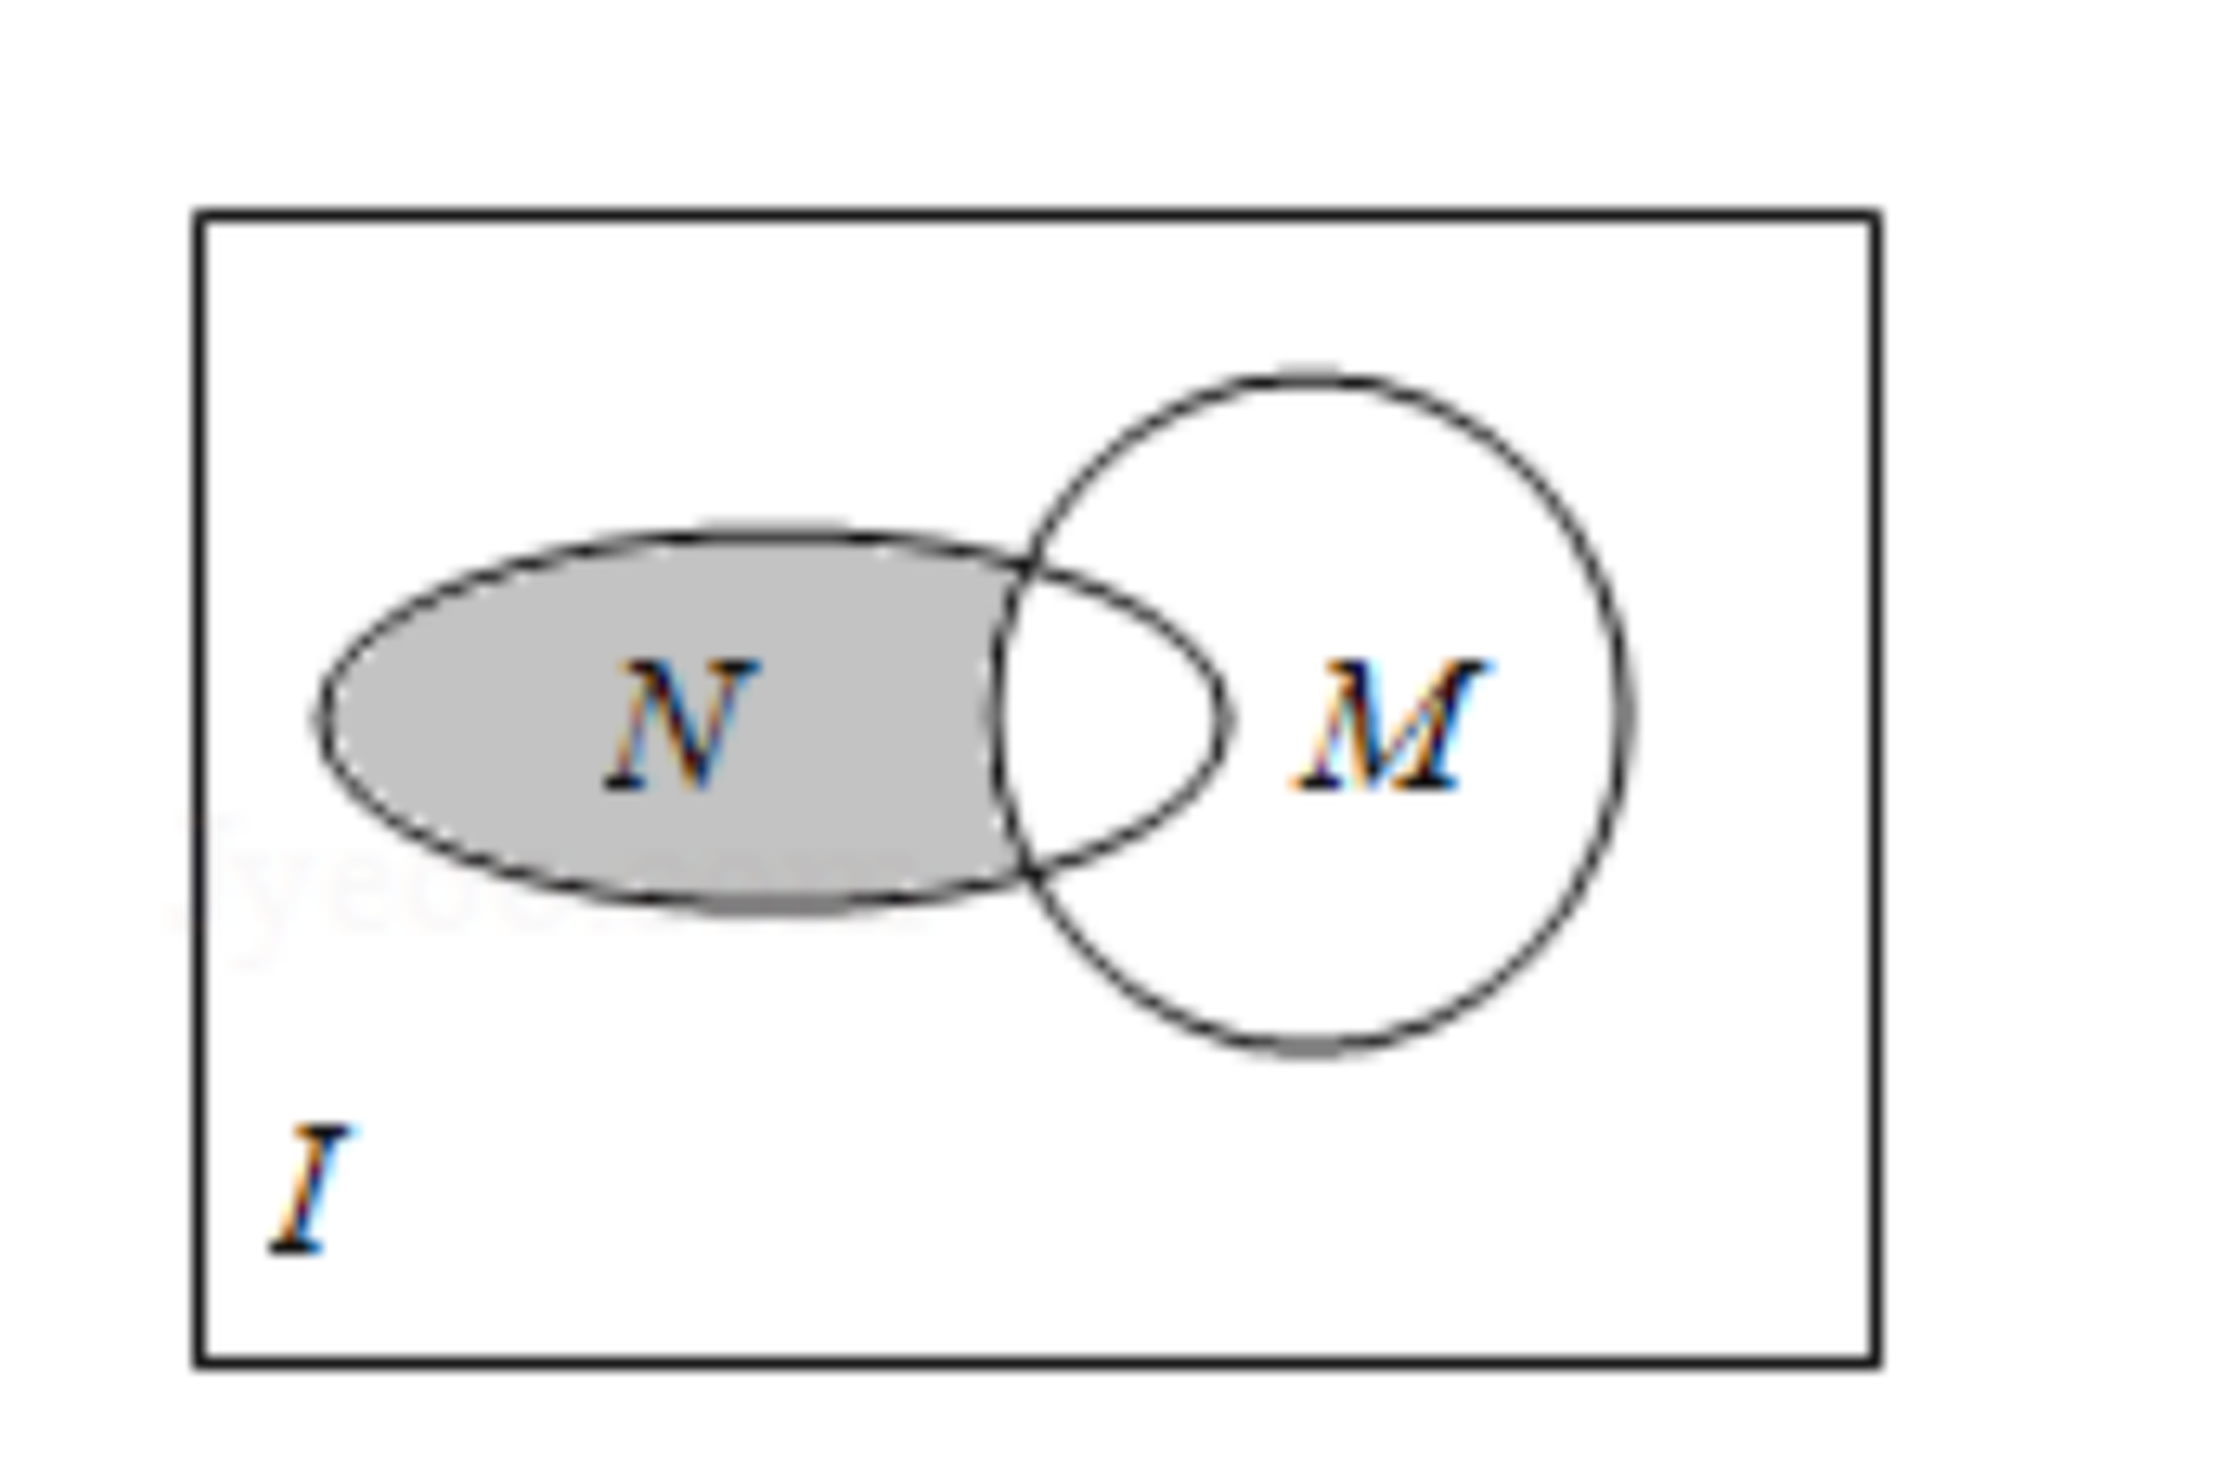
\includegraphics[width=0.30\textwidth]{figures/venn_N_cap_CI_M_h39.png}
\end{center}

\ans{$[-3,-\sqrt3)$}

\ifanswer
\solbegin
\step{阴影部分用集合表示为 $N\cap(\complement_UM)$.}
\step{则 $M=\{x\mid y=\sqrt{3-x^2}\}=\{x\mid3-x^2\geqslant0\}=\{x\mid-\sqrt3\leqslant x\leqslant\sqrt3\}$，}
\step{则 $\complement_UM=\{x\mid x>\sqrt3\text{ 或 }x<-\sqrt3\}$，$N=\{x\mid|x+1|\leqslant2\}=\{x\mid-3\leqslant x\leqslant1\}$，}
\step{则 $N\cap(\complement_UM)=\{x\mid-3\leqslant x<-\sqrt3\}$.}
\solend

\fi

\item 已知 $f(x)=x^2+ax+b$，集合 $\{x\mid f(x)=x\}=\{4\}$，将集合 $M=\{x\mid f(x)=4\}$ 用列举法表示 \blankline[4.4em].

\ans{$\{3,4\}$}

\ifanswer
\solbegin
\step{已知 $f(x)=x^2+ax+b$，集合 $\{x\mid f(x)=x\}=\{4\}$，}
% 注：原卷本行作「…$x^2+(a-1)x+b=0$ **由**两个相等的实数根为 $4$」——「由」当为「有」
%     （「设…是…有」的杂糅）；本稿照录未改，见文件头「原卷笔误/存疑」⑧。
\step{即方程 $x^2+ax+b=x$，$x^2+(a-1)x+b=0$ 由两个相等的实数根为 $4$，}
\step{所以 $\triangle=(a-1)^2-4b=0$，即 $x^2+(a-1)x+b=(x-4)^2$，所以 $b=16$，$a=-7$，}
\step{所以 $f(x)=x^2+ax+b=x^2-7x+16$，所以集合 $M=\{x\mid f(x)=4\}$，}
\step{即 $x^2-7x+16=4$，$x^2-7x+12=0$，故 $M=\{x\mid f(x)=4\}=\{3,4\}$.}
\solend

\fi

% 注：原卷方程组第二式印作 $1-2<-k\leqslant3$，按其结论 $-3\leqslant k<2$ 反推疑当作 $-2<-k\leqslant3$，
%     照录未改，见文件头「笔误/存疑」③。
\item 关于 $x$ 的不等式组 $\begin{cases}x^2-x-2>0\\ 2x^2+(2k+5)x+5k<0\end{cases}$ 的整数解的集合为 $\{-2\}$，
则实数 $k$ 的取值范围 \blankline[4.4em].

\ans{$-3\leqslant k<2$}

\ifanswer
\solbegin
\step{原不等式组即 $\begin{cases}(x-2)(x+1)>0\\ (x+k)(2x+5)<0\end{cases}$，整数解的集合为 $A$，若 $A=\{-2\}$，}
\step{则 $(-2+k)(2\times(-2)+5)<0$，所以 $k<2$，且有 $\begin{cases}-k>-\dfrac52\\ 1-2<-k\leqslant3\end{cases}$，}
\step{解得 $-3\leqslant k<2$.}
\solend

\fi

\item 规定 $\oplus$ 与 $\otimes$ 是两个运算符号，其运算法则如下，对任意实数 $a$、$b$ 有：$a\otimes b=ab$，
$a\oplus b=b(a^2+b^2+1)$. 若 $-2<a<b<2$ 且 $a$、$b\in\Z$，
$A=\left\{x\mid x=2(a\otimes b)+\dfrac{a\oplus b}{2b}\right\}$，则用列举法表示集合 $A=$ \blankline[4.4em].

\ans{$\left\{1,-\dfrac12\right\}$}

\ifanswer
\solbegin
\step{$A=\left\{x\mid x=2(a\otimes b)+\dfrac{a\oplus b}{2b}\right\}
=\left\{x\mid x=2ab+\dfrac{b(a^2+b^2+1)}{2b}\right\}$}
\step{$=\left\{x\mid x=2ab+\dfrac12a^2+\dfrac12b^2+\dfrac12\right\}
=\left\{x\mid x=\dfrac12(a+b)^2+ab+\dfrac12\right\}$，}
% 注：题设含 $\dfrac{a\oplus b}{2b}$，而 $-2<a<b<2$、$a$、$b\in\Z$ 时 $(a,b)=(-1,0)$ 也合条件、
%     却使分母 $2b=0$；原卷解析仍代入该组并约去 $b$ 得 $x=1$（答案集恰好不变）。本稿照录，
%     见文件头「原卷笔误/存疑」⑨。
\step{当 $a=-1$，$b=0$ 时，$x=1$；当 $a=-1$，$b=1$ 时，$x=-\dfrac12$；}
\step{当 $a=0$，$b=1$ 时，$x=1$；所以 $A=\left\{1,-\dfrac12\right\}$.}
\solend

\fi

\item 高斯是德国著名的数学家，近代数学奠基者之一，享有“数学王子”的称号，为了纪念数学家高斯，
我们把取整函数 $y=[x]$，$x\in\R$ 称为高斯函数，其中 $[x]$ 表示不超过 $x$ 的最大整数，
如 $[1.1]=1$，$[-1.1]=-2$. 则点集 $P=\{(x,y)\mid[x]^2+[y]^2=1\}$
所表示的平面区域的面积是 \blankline[4.4em].

\ans{$4$}

\ifanswer
\solbegin
\step{$[x]^2+[y]^2=1$ 由 $\begin{cases}[x]=0\\ [y]=-1\end{cases}$ 或 $\begin{cases}[x]=0\\ [y]=1\end{cases}$
或 $\begin{cases}[x]=-1\\ [y]=0\end{cases}$ 或 $\begin{cases}[x]=1\\ [y]=0\end{cases}$ 四个平面区域组成，}
\step{即 $\begin{cases}0\leqslant x<1\\ -1\leqslant y<0\end{cases}$ 或 $\begin{cases}0\leqslant x<1\\ 1\leqslant y<2\end{cases}$
或 $\begin{cases}-1\leqslant x<0\\ 0\leqslant y<1\end{cases}$ 或 $\begin{cases}1\leqslant x<2\\ 0\leqslant y<1\end{cases}$，}
\step{作出平面区域如图所示，平面区域由四个边长为 $1$ 的正方形组成，}
% 图在【解析】内（仅答案版出），取原卷截图（03.png，2560×3620）中部，4× LANCZOS 放大。
\begin{center}
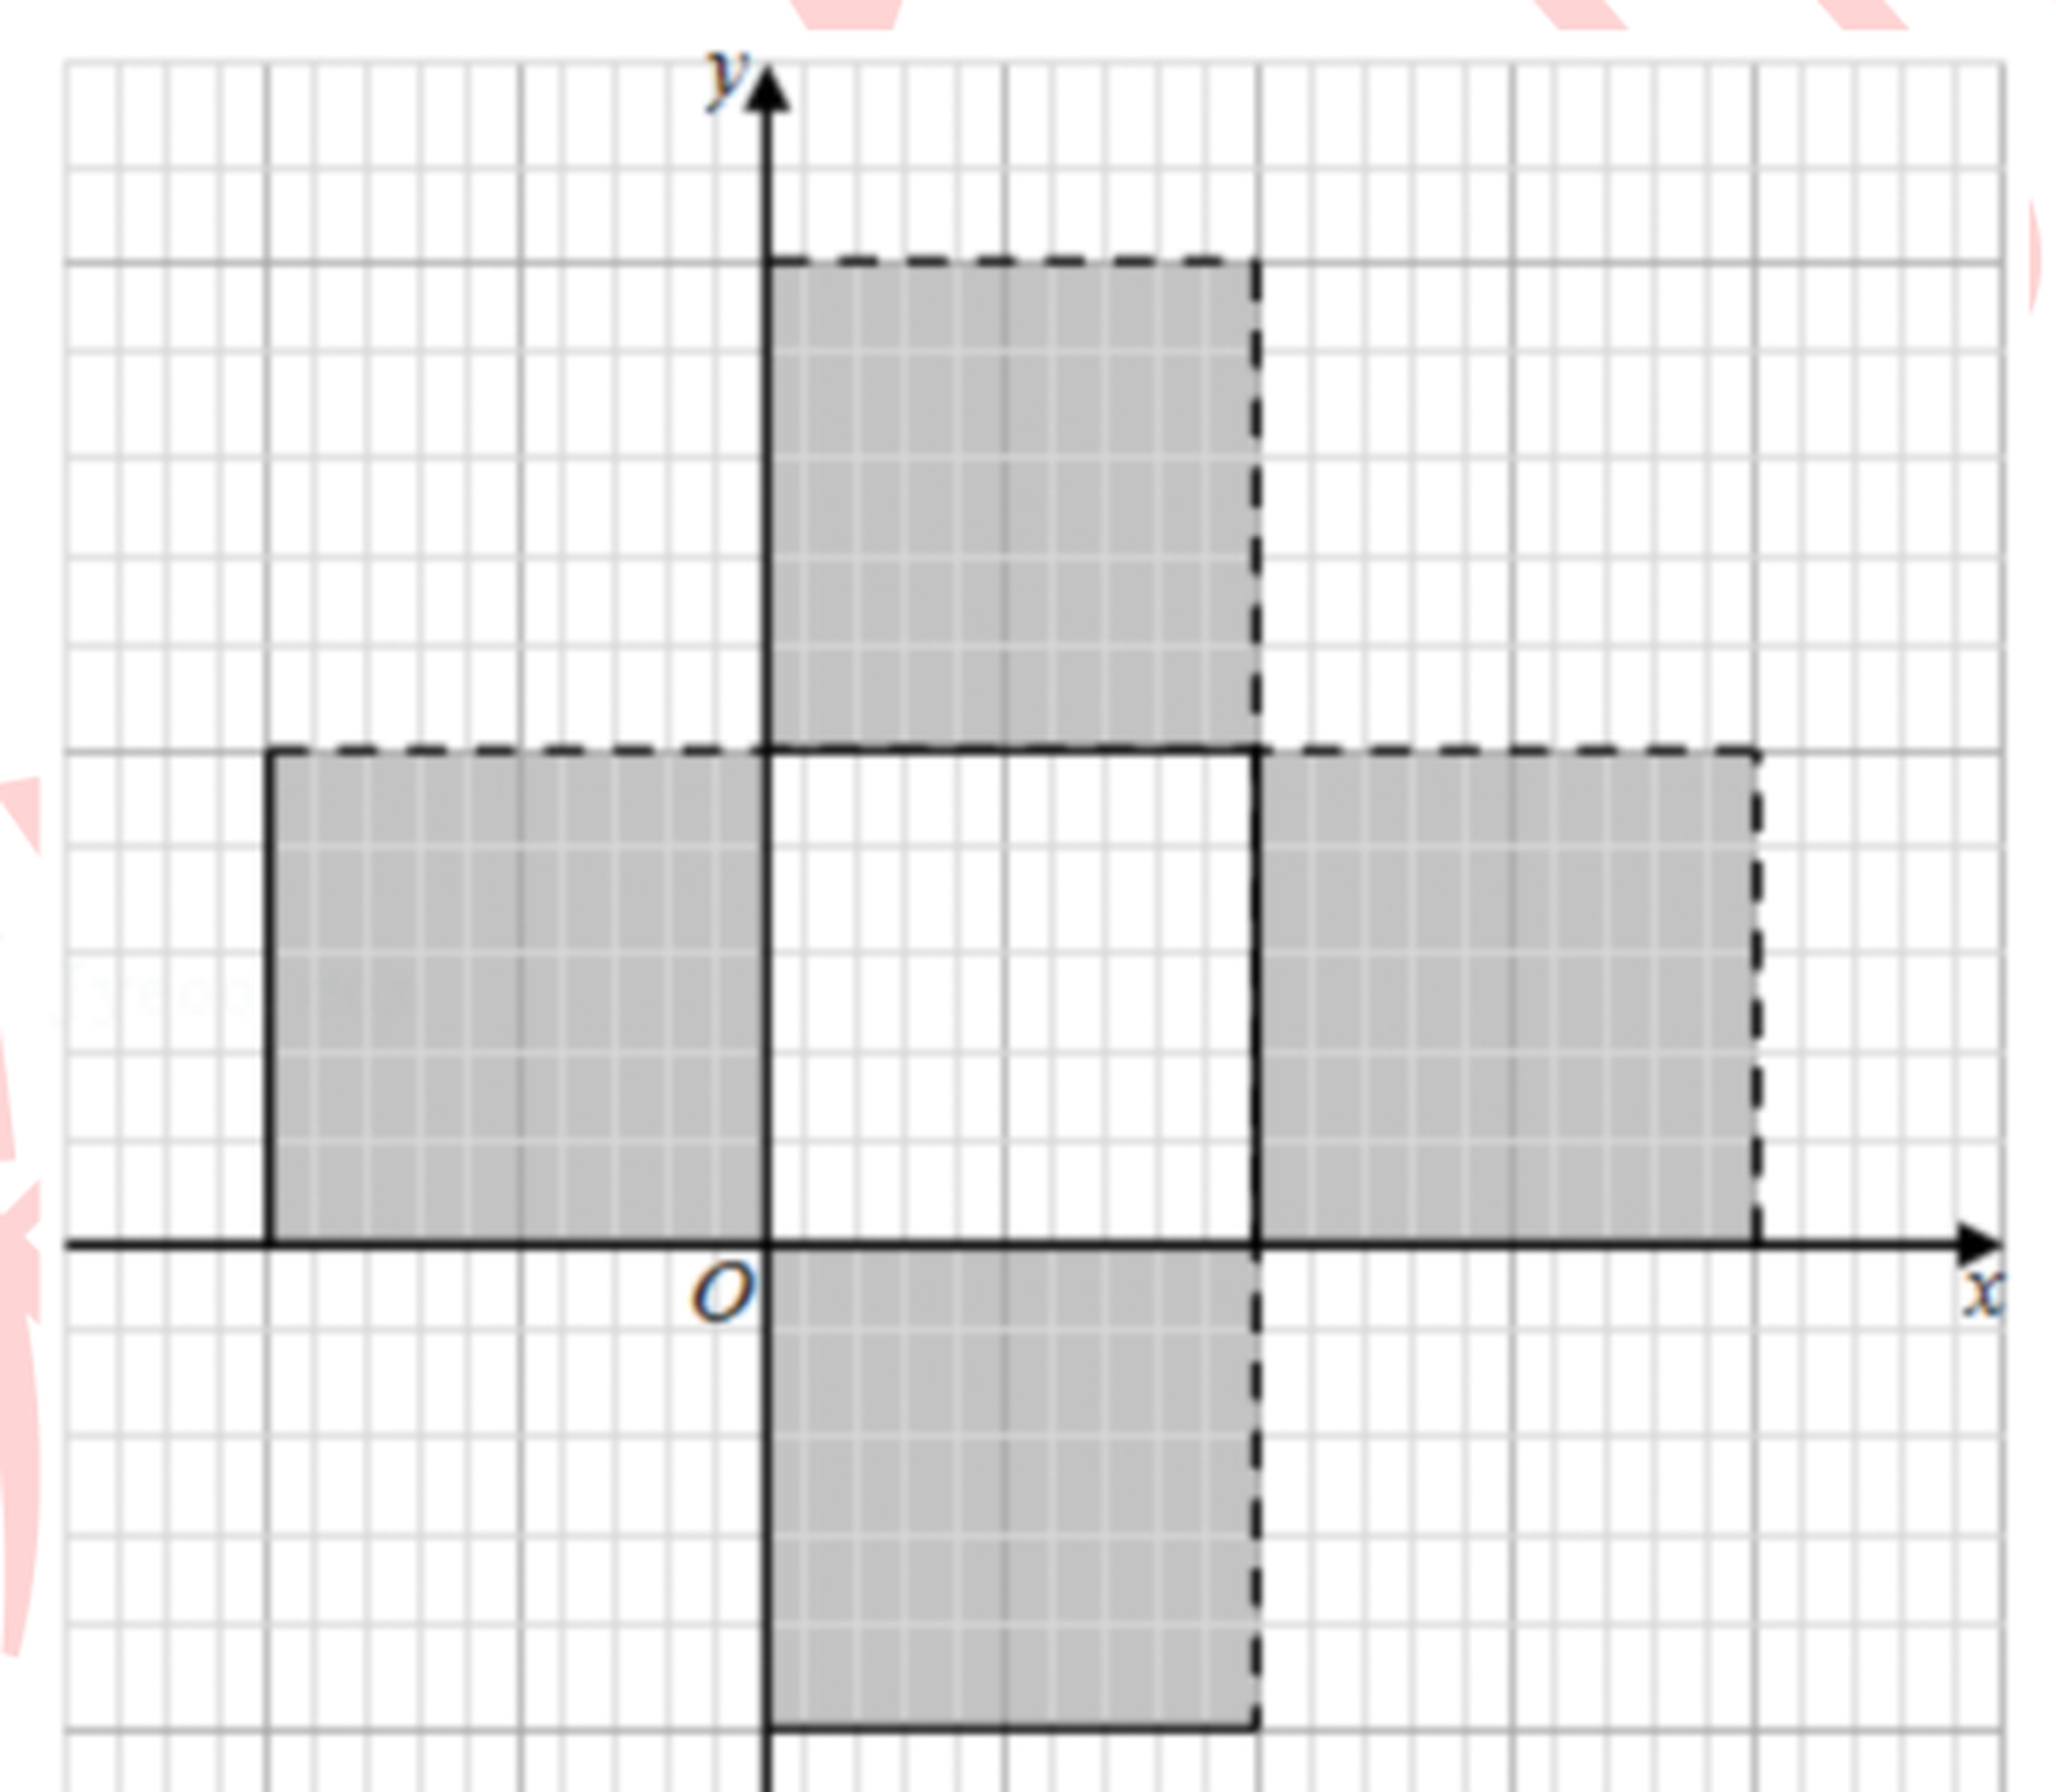
\includegraphics[width=0.38\textwidth]{figures/plane_grid_4squares_h39.png}
\end{center}
\step{总面积为 $1\times4=4$.}
\solend

\fi

\item 关于 $x$ 的不等式 $ax^2+bx+c>0$ 的解集为 $\{x\mid x<\beta\text{ 或 }x>\gamma\}(0<\beta<\gamma)$，
则不等式 $a(x^2+1)+b(x-1)+c>2ax$ 的解集为 \blankline[4.4em].

\ans{$(-\infty,\beta+1)\cup(\gamma+1,+\infty)$}

\ifanswer
\solbegin
\step{由题意得 $\beta$、$\gamma$ 为方程 $ax^2+bx+c=0$ 的两根且 $a>0$，}
\step{则 $\beta+\gamma=-\dfrac ba$，$\beta\gamma=\dfrac ca$，故 $b=-a(\beta+\gamma)$，$c=\beta\gamma a$，}
\step{则不等式可化为 $a(x^2+1)-a(\beta+\gamma)(x-1)+\beta\gamma a>2ax$，}
\step{因为 $a>0$，所以 $x^2+1-(\beta+\gamma)(x-1)+\beta\gamma>2x$，}
\step{即 $x^2-(\beta+\gamma+2)x+(\beta+\gamma+\beta\gamma+1)>0$，所以 $(x-\beta-1)(x-\gamma-1)>0$，}
\step{解得 $x<\beta+1$ 或 $x>\gamma+1$，所以不等式解集为 $(-\infty,\beta+1)\cup(\gamma+1,+\infty)$.}
\solend

\fi

\end{enumerate}

\bigsec{二、选择题}

\begin{enumerate}
\setcounter{enumi}{12}

\item 设 $a<b<0$，则下列不等式中不成立的是\mbox{（\quad）}

\keepwithprev
A. $\dfrac1a>\dfrac1b$\qquad B. $\dfrac{1}{a-b}>\dfrac1a$\qquad C. $|a|>-b$\qquad D. $\sqrt{-a}>\sqrt{-b}$

\ans{$B$}

\ifanswer
\solbegin
\step{令 $a=-2$，$b=-1$，}
\step{A、$-\dfrac12>-1$，正确；B、$-1<-\dfrac12$，故 B 错误；C、$2>1$，正确；}
\step{D、$\sqrt2>1$，正确；故选 B.}
\solend

\fi

\item 设实数集 $\R$ 为全集，集合 $P=\{x\mid f(x)=0\}$，$Q=\{x\mid g(x)=0\}$，$H=\{x\mid h(x)=0\}$，
则方程 $\dfrac{f^2(x)+g^2(x)}{h(x)}=0$ 的解集是\mbox{（\quad）}

\keepwithprev
A. $P\cap Q\cap\overline{H}$\qquad B. $P\cap Q$\qquad C. $P\cap Q\cap H$\qquad D. $P\cap Q\cup H$

\ans{$A$}

\ifanswer
\solbegin
\step{方程 $\dfrac{f^2(x)+g^2(x)}{h(x)}=0$ 等价于 $\begin{cases}f(x)=0\\ g(x)=0\\ h(x)\neq0\end{cases}$，}
\step{又因为 $P=\{x\mid f(x)=0\}$，$Q=\{x\mid g(x)=0\}$，$H=\{x\mid h(x)=0\}$，}
\step{所以方程 $\dfrac{f^2(x)+g^2(x)}{h(x)}=0$ 的解集是 $P\cap Q\cap\overline{H}$，故选 A.}
\solend

\fi

\item 设全集 $U$，在下列条件中，是 $B\sub A$ 的充要条件的有\mbox{（\quad）}

\keepwithprev
% 注：原卷此行 ② 与 ③ 之间**漏排分隔号**（①、③ 后都有「；」，② 后没有）；
%     本稿照录未补，见文件头「原卷笔误/存疑」⑩。
①$A\cup B=A$；\qquad ②$\overline{A}\cap B=\varnothing$\qquad ③$\overline{A}\sub\overline{B}$；\qquad ④$A\cup\overline{B}=U$

\keepwithprev
A. $1$ 个\qquad B. $2$ 个\qquad C. $3$ 个\qquad D. $4$ 个

\ans{$D$}

\item 已知集合 $M=\{x\mid x\in\N,0<x\leqslant15\}$，$A_1$、$A_2$、$A_3$ 满足：①$A_1\cup A_2\cup A_3=M$；
②每个集合都恰有 $5$ 个元素. 集合 $A_i(i=1,2,3)$ 中最大元素与最小元素之和称为 $A_i$ 的特征数，
记为 $X_i(i=1,2,3)$，则 $X_1+X_2+X_3$ 的值不可能为\mbox{（\quad）}

\keepwithprev
A. $37$\qquad B. $39$\qquad C. $48$\qquad D. $57$

\ans{$A$}

\ifanswer
\solbegin
\step{因为集合 $M=\{x\mid x\in\N,0<x\leqslant15\}=\{1,2,3,\cdots,15\}$，}
\step{又因为集合 $A_1$、$A_2$、$A_3$ 中，每个集合恰有 $5$ 个元素，}
\step{且 $A_1\cup A_2\cup A_3=M$ 有 $15$ 个元素，所以集合 $A_1$、$A_2$、$A_3$ 中没有重复元素，}
\step{因为 $1$ 是集合 $M$ 中数值最小的元素，$15$ 是集合 $M$ 中数值最大的元素，}
\step{所以在 $A_i$ 的特征数构成中，必有 $1$ 和 $15$，不妨设 $1\in A_1$，$15\in A_1$，}
% 注：原卷本行（与下面「最小」那句）在「集合」后的角标是**数字 $1$**（同句 $X_1$ 的角标同形），
%     而非上一行「$A_i$ 的特征数构成」里的斜体 $A_i$——原卷两种下标并存，本稿照录、不归一，
%     见文件头「原卷笔误/存疑」⑬。
\step{要使 $X_1+X_2+X_3$ 最大，则应该在集合 $A_1$ 中首先放置数值较小的元素，}
\step{即 $A_1=\{1,2,3,4,15\}$，所以 $5$ 与 $14$ 是剩下元素中数值最小或最大的元素，}
\step{同理，不妨设 $5\in A_2$，$14\in A_2$，接着在 $A_2$ 中再次放置数值较小的元素，}
\step{即 $A_2=\{5,6,7,8,14\}$，则 $A_3=\{9,10,11,12,13\}$，}
\step{此时 $X_1+X_2+X_3$ 有最大值为 $1+15+5+14+9+13=57$，}
\step{即 $X_1+X_2+X_3\leqslant57$；}
% 注：同上一处——原卷此行角标是**数字 $1$**（$A_1$），本稿照录，未与「$A_i$」归一。
\step{要使 $X_1+X_2+X_3$ 最小，则在集合 $A_1$ 中首先放置数值较大的元素，}
\step{即 $A_1=\{1,12,13,14,15\}$，所以 $2$ 与 $11$ 是剩下元素中数值最小或最大的元素，}
\step{同理，不妨设 $2\in A_2$，$11\in A_2$，接着在 $A_2$ 中再次放置数值较大的元素，}
\step{即 $A_2=\{2,8,9,10,11\}$，则 $A_3=\{3,4,5,6,7\}$，}
\step{此时 $X_1+X_2+X_3$ 有最小值为 $1+15+2+11+3+7=39$，}
\step{即 $X_1+X_2+X_3\geqslant39$，}
\step{综上，$39\leqslant X_1+X_2+X_3\leqslant57$，故选 A.}
\solend

\fi

\end{enumerate}

\bigsec{三、解答题}

\begin{enumerate}
\setcounter{enumi}{16}

% 注：原卷首句「由数 $y=-x^2+ax-1=-x+3$」中的「由数」显系「由」或「由函数」之误；末段
%     的两处分类讨论与结论自相矛盾（详见文件头「笔误/存疑」④）。本稿一律照录，未改。
\item 命题 $p$：函数 $y=-x^2+ax-1$ 与 $y=-x+3$ 图象交点的横坐标均为负值，
命题 $q$：关于 $x$ 的方程 $2(1-x)a+(x^2-10x-3)=0$ 的两个根，一个大于 $3$，另一个小于 $3$；
若命题 $p$ 和命题 $q$ 中有且仅有一个是真命题，求 $a$ 的取值范围.

\ans{$\R$}

\ifanswer
\solbegin
\step{由数 $y=-x^2+ax-1=-x+3$ 得 $x^2-(a+1)x+4=0$，}
\step{若横坐标均为负值，则满足 $\begin{cases}\Delta=(a+1)^2-16\geqslant0\\ x_1x_2=4>0\\ x_1+x_2=a+1<0\end{cases}$
得 $\begin{cases}a\geqslant3\text{ 或 }a\leqslant-5\\ a<-1\end{cases}$，得 $a\leqslant-5$，}
\step{即 $p:a\leqslant-5$，}
\step{若方程 $2(1-x)a+(x^2-10x-3)=0$ 的两个根，一个大于 $3$，另一个小于 $3$；}
\step{设 $f(x)=2(1-x)a+(x^2-10x-3)$，则 $f(3)<0$，即 $-4a-24<0$，}
\step{得 $a>-6$，即 $q:a>-6$，}
\step{因为命题 $p$ 和命题 $q$ 中有且仅有一个是真命题，}
\step{若 $p$ 真 $q$ 假，则 $\begin{cases}a\leqslant-5\\ a>-6\end{cases}$，得 $a\in\R$，}
\step{若 $p$ 假 $q$ 真，则 $\begin{cases}a>-5\\ a\leqslant-6\end{cases}$，此时 $a$ 无解，}
\step{综上，实数 $a$ 的取值范围是 $\R$.}
\solend

\fi

\ansspace[8]

\item 设全集是实数集 $\R$，$A=\left\{x\mid\dfrac{1-2x}{x-3}\geqslant0\right\}$，$B=\{x\mid x^2+a\leqslant0\}$.

\begin{enumerate}[label=(\arabic*)]

\item 当 $a=-4$ 时，求 $A\cup B$；

\item 若 $\overline{A}\cap B=B$，求实数 $a$ 的取值范围.

\end{enumerate}

\ans{（1）$\{x\mid-2\leqslant x<3\}$；（2）$\left(-\dfrac14,+\infty\right)$}

\ifanswer
\solbegin
\stepm{(1)}{$A=\left\{x\mid\dfrac{1-2x}{x-3}\geqslant0\right\}=\left\{x\mid\dfrac12\leqslant x<3\right\}$，$B=\{x\mid x^2+a\leqslant0\}$.}
\step{当 $a=-4$ 时，$B=\{x\mid-2\leqslant x\leqslant2\}$，所以 $A\cup B=\{x\mid-2\leqslant x<3\}$.}
\stepm{(2)}{$\overline{A}=\left\{x\mid x\geqslant3\text{ 或 }x<\dfrac12\right\}$，$B=\{x\mid x^2+a\leqslant0\}$.}
\step{由 $\overline{A}\cap B=B$，得 $B\sub\overline{A}$，}
\step{则当 $a>0$ 时，$B=\varnothing$，满足 $B\sub\overline{A}$，则 $a>0$ 成立，}
\step{则当 $a=0$ 时，$B=\{0\}$，满足 $B\sub\overline{A}$，则 $a=0$ 成立，}
\step{当 $a<0$ 时，$B=\{x\mid-\sqrt{-a}\leqslant x<\sqrt{-a}\}$，}
\step{得 $\sqrt{-a}<\dfrac12$，即 $-\dfrac14<a<0$，}
\step{综上，实数 $a$ 的取值范围是 $\left(-\dfrac14,+\infty\right)$.}
\solend

\fi

\ansspace[6]

\item 设集合 $A=\{x\mid ax^2+2x+1=0,a\in\R\}$.

\begin{enumerate}[label=(\arabic*)]

\item 当 $A$ 中元素个数为 $1$ 时，求：$a$ 和 $A$；

\item 当 $A$ 中元素个数至少为 $1$ 时，求：$a$ 的取值范围；

\item 求：$A$ 中各元素之和.

\end{enumerate}

\ans{（1）$a=0$ 时 $A=\left\{-\dfrac12\right\}$，$a=1$ 时 $A=\{-1\}$；（2）$(-\infty,1]$；
（3）$a=0$ 时和为 $-\dfrac12$，$a<1$ 且 $a\neq0$ 时和为 $-\dfrac2a$，$a=1$ 时和为 $-1$，$a>1$ 时 $A$ 中无元素}

\ifanswer
\solbegin
\stepm{(1)}{集合 $A=\{x\mid ax^2+2x+1=0,a\in\R\}$，$A$ 中元素个数为 $1$，}
\step{所以 $a=0$ 或 $\begin{cases}a\neq0\\ \Delta=4-4a=0\end{cases}$，解得 $a=0$，$A=\left\{-\dfrac12\right\}$ 或 $a=1$，$A=\{-1\}$.}
\stepm{(2)}{当 $A$ 中元素个数至少为 $1$ 时，$a=0$ 或 $\begin{cases}a\neq0\\ \Delta=4-4a\geqslant0\end{cases}$，解得 $a\leqslant1$，}
\step{所以 $a$ 的取值范围是 $(-\infty,1]$.}
\stepm{(3)}{当 $a=0$ 时，$A$ 中元素之和为 $-\dfrac12$；}
\step{当 $a<1$ 且 $a\neq0$ 时，$A$ 中元素之和为 $-\dfrac2a$；}
\step{当 $a=1$ 时，$A$ 中元素之和为 $-1$；}
\step{当 $a>1$ 时，$A$ 中无元素.}
\solend

\fi

\ansspace[8]

\item 设 $k$ 是正整数，集合 $A$ 至少有两个元素，且 $A\sub\N^*$. 如果对于 $A$ 中的任意两个不同的
元素 $x$、$y$，都有 $|x-y|\neq k$，则称 $A$ 具有性质 $P(k)$.

\begin{enumerate}[label=(\arabic*)]

\item 试判断集合 $B=\{1,2,3,4\}$ 和 $C=\{1,4,7,10\}$ 是否具有性质 $P(2)$？并说明理由；

\item 若集合 $A=\{a_1,a_2,\cdots,a_{12}\}\sub\{1,2,\cdots,20\}$，求证：$A$ 不可能具有性质 $P(3)$；

\item 若集合 $A\sub\{1,2,\cdots,2023\}$，且同时具有性质 $P(4)$ 和 $P(7)$，求集合 $A$ 中元素个数的
最大值.

\end{enumerate}

\ans{（1）$B$ 不具有性质 $P(2)$，$C$ 具有性质 $P(2)$；（2）见解析；（3）$920$}

\ifanswer
\solbegin
\stepm{(1)}{因为 $B=\{1,2,3,4\}$，}
\step{又 $1\in\N^*$，$2\in\N^*$，$3\in\N^*$，$4\in\N^*$，但 $|4-2|=2$，}
\step{所以集合 $B$ 不具有性质 $P(2)$，}
\step{因为 $C=\{1,4,7,10\}$，}
\step{又 $1\in\N^*$，$4\in\N^*$，$7\in\N^*$，$10\in\N^*$，}
\step{但 $|4-1|=3$，$|7-1|=6$，$|10-1|=9$，$|7-4|=3$，$|10-4|=6$，$|10-7|=3$，}
\step{所以集合 $C$ 具有性质 $P(2)$，}
\stepm{(2)}{将集合 $\{1,2,\cdots,20\}$ 中的元素分为如下 $11$ 个集合，}
% 注：原卷本行 $\{8,11\}$ 与 $\{9,12\}$ 之间的分隔号误用**句号**「.」（同行其余处皆逗号），
%     本稿照录、未改，见文件头「原卷笔误/存疑」⑪。
\step{$\{1,4\}$，$\{2,5\}$，$\{3,6\}$，$\{7,10\}$，$\{8,11\}$.$\{9,12\}$，$\{13,16\}$，$\{14,17\}$，$\{15,18\}$，}
\step{$\{19\}$，$\{20\}$，}
\step{所以从集合 $\{1,2,\cdots,20\}$ 中取 $12$ 个元素，则前 $9$ 个集合至少要选 $10$ 个元素，}
\step{所以必有 $2$ 个元素取自前 $9$ 个集合中的同一集合，即存在两个元素其差为 $3$，}
\step{所以 $A$ 不可能具有性质 $P(3)$；}
\stepm{(3)}{先说明连续 $11$ 项中集合 $A$ 中最多选取 $5$ 项，}
\step{以 $1,2,3,\cdots,11$ 为例.}
\step{构造抽屉 $\{1,8\}$，$\{2,9\}$，$\{3,10\}$，$\{4,11\}$，$\{5\}$，$\{6\}$，$\{7\}$.}
\step{①$5$、$6$、$7$ 同时选，因为具有性质 $P(4)$ 和 $P(7)$，}
\step{所以选 $5$ 则不选 $1$、$9$；选 $6$ 则不选 $2$、$10$；选 $7$ 则不选 $3$、$11$；}
% 注：原卷此步推理不严——「只剩 $4$、$8$」但两数相差 $4$、不能同选，该情形实际最多只能取 $4$ 个；
%     末句「不超过 $5$ 个」的结论仍成立。本稿照录，见文件头「原卷笔误/存疑」⑫。
\step{则只剩 $4$、$8$；故 $1,2,3,\cdots,11$ 中属于集合 $A$ 的元素个数不超过 $5$ 个.}
\step{②$5$、$6$、$7$ 选 $2$ 个，}
\step{若只选 $5$、$6$，则 $1$、$2$、$9$、$10$、$7$ 不可选，又 $\{4,11\}$ 只能选一个元素，}
\step{$3$、$8$ 可以选，故 $1,2,3,\cdots,11$ 中属于集合 $A$ 的元素个数不超过 $5$ 个.}
\step{若选 $5$、$7$，则只能从 $2$、$4$、$8$、$10$ 中选，但 $4$、$8$ 不能同时选，}
\step{故 $1,2,3,\cdots,11$ 中属于集合 $A$ 的元素个数不超过 $5$ 个.}
\step{若选 $6$、$7$，则 $2$、$3$、$10$、$11$、$5$ 不可选，又 $\{1,8\}$ 只能选一个元素，}
\step{$4$、$9$ 可以选，故 $1,2,3,\cdots,11$ 中属于集合 $A$ 的元素个数不超过 $5$ 个.}
\step{③$5$、$6$、$7$ 中只选 $1$ 个，}
\step{又四个集合 $\{1,8\}$，$\{2,9\}$，$\{3,10\}$，$\{4,11\}$ 每个集合至多选 $1$ 个元素，}
\step{故 $1,2,3,\cdots,11$ 中属于集合 $A$ 的元素个数不超过 $5$ 个.}
\step{由上述①②③得，连续 $11$ 项自然数中属于集合 $A$ 的元素至多只有 $5$ 个，}
\step{如取 $1$、$4$、$6$、$7$、$9$.}
\step{因为 $2023=183\times11+10$，则把每 $11$ 个连续自然数分组，}
\step{前 $183$ 组每组至多选取 $5$ 项；}
\step{从 $2014$ 开始，最后 $10$ 个数至多选取 $5$ 项，}
\step{故集合 $A$ 的元素最多有 $184\times5=920$ 个.}
\step{给出如下选取方法：从 $1,2,3,\cdots,11$ 中选取 $1$、$4$、$6$、$7$、$9$；}
\step{然后在这 $5$ 个数的基础上每次累加 $11$，构造 $183$ 次.}
\step{此时集合 $A$ 的元素为 $1$，$4$，$6$，$7$，$9$；$12$，$15$，$17$，$18$，$20$；$23$，$26$，$28$，$29$，$31$；
$\cdots$；$2014$，$2017$，$2019$，$2020$，$2022$，共 $920$ 个元素.}
\step{经检验得该集合符合要求，故集合 $A$ 的元素最多有 $920$ 个.}
\solend

\fi

\ansspace[10]

\end{enumerate}

\bigsec{附加题}

\begin{enumerate}
\setcounter{enumi}{20}

\item 若规定集合 $M=\{a_1,a_2,\cdots,a_n\}$（$n\in\N^*$）的子集 $\{a_{i_1},a_{i_2},\cdots,a_{i_m}\}$（$m\in\N^*$）
为 $M$ 的第 $k$ 个子集，其中 $k=2^{i_1-1}+2^{i_2-1}+\cdots+2^{i_m-1}$，则 $M$ 的第 $25$ 个子集是 \blankline[4.4em].

\ans{$\{a_1,a_4,a_5\}$}

\ifanswer
\solbegin
\step{由题意得 $M$ 的第 $k$ 个子集，且 $k=2^{i_1-1}+2^{i_2-1}+\cdots+2^{i_m-1}$，}
\step{又 $25=2^0+2^3+2^4=2^{1-1}+2^{4-1}+2^{5-1}$，所以 $M$ 的第 $25$ 个子集是 $\{a_1,a_4,a_5\}$.}
\solend

\fi

% 注：原卷在 $x=1$、$y=2$、$z=3$ 时把 $B=\{x,y\}$ 印作 $\{1,3\}$（应为 $\{1,2\}$），
%     照录未改，见文件头「笔误/存疑」⑥。
\item 用 $|S|$ 表示集合 $S$ 中的元素的个数，设 $A$、$B$、$C$ 为集合，称 $(A,B,C)$ 为有序三元组.
如果集合 $A$、$B$、$C$ 满足 $|A\cap B|=|B\cap C|=|C\cap A|=1$，且 $A\cap B\cap C=\varnothing$，
则称有序三元组 $(A,B,C)$ 为最小相交. 由集合 $\{1,2,3\}$ 的子集构成的所有有序三元组中，
最小相交的有序三元组的个数为 \blankline[4.4em].

\ans{$6$}

\ifanswer
\solbegin
\step{因为 $|A\cap B|=|B\cap C|=|C\cap A|=1$，}
\step{所以设 $A\cap B=\{x\}$，$B\cap C=\{y\}$，$C\cap A=\{z\}$，}
% 图在【解析】内（仅答案版出），取原卷截图（10.png，2560×3620）右栏，4× LANCZOS 放大。
\begin{center}
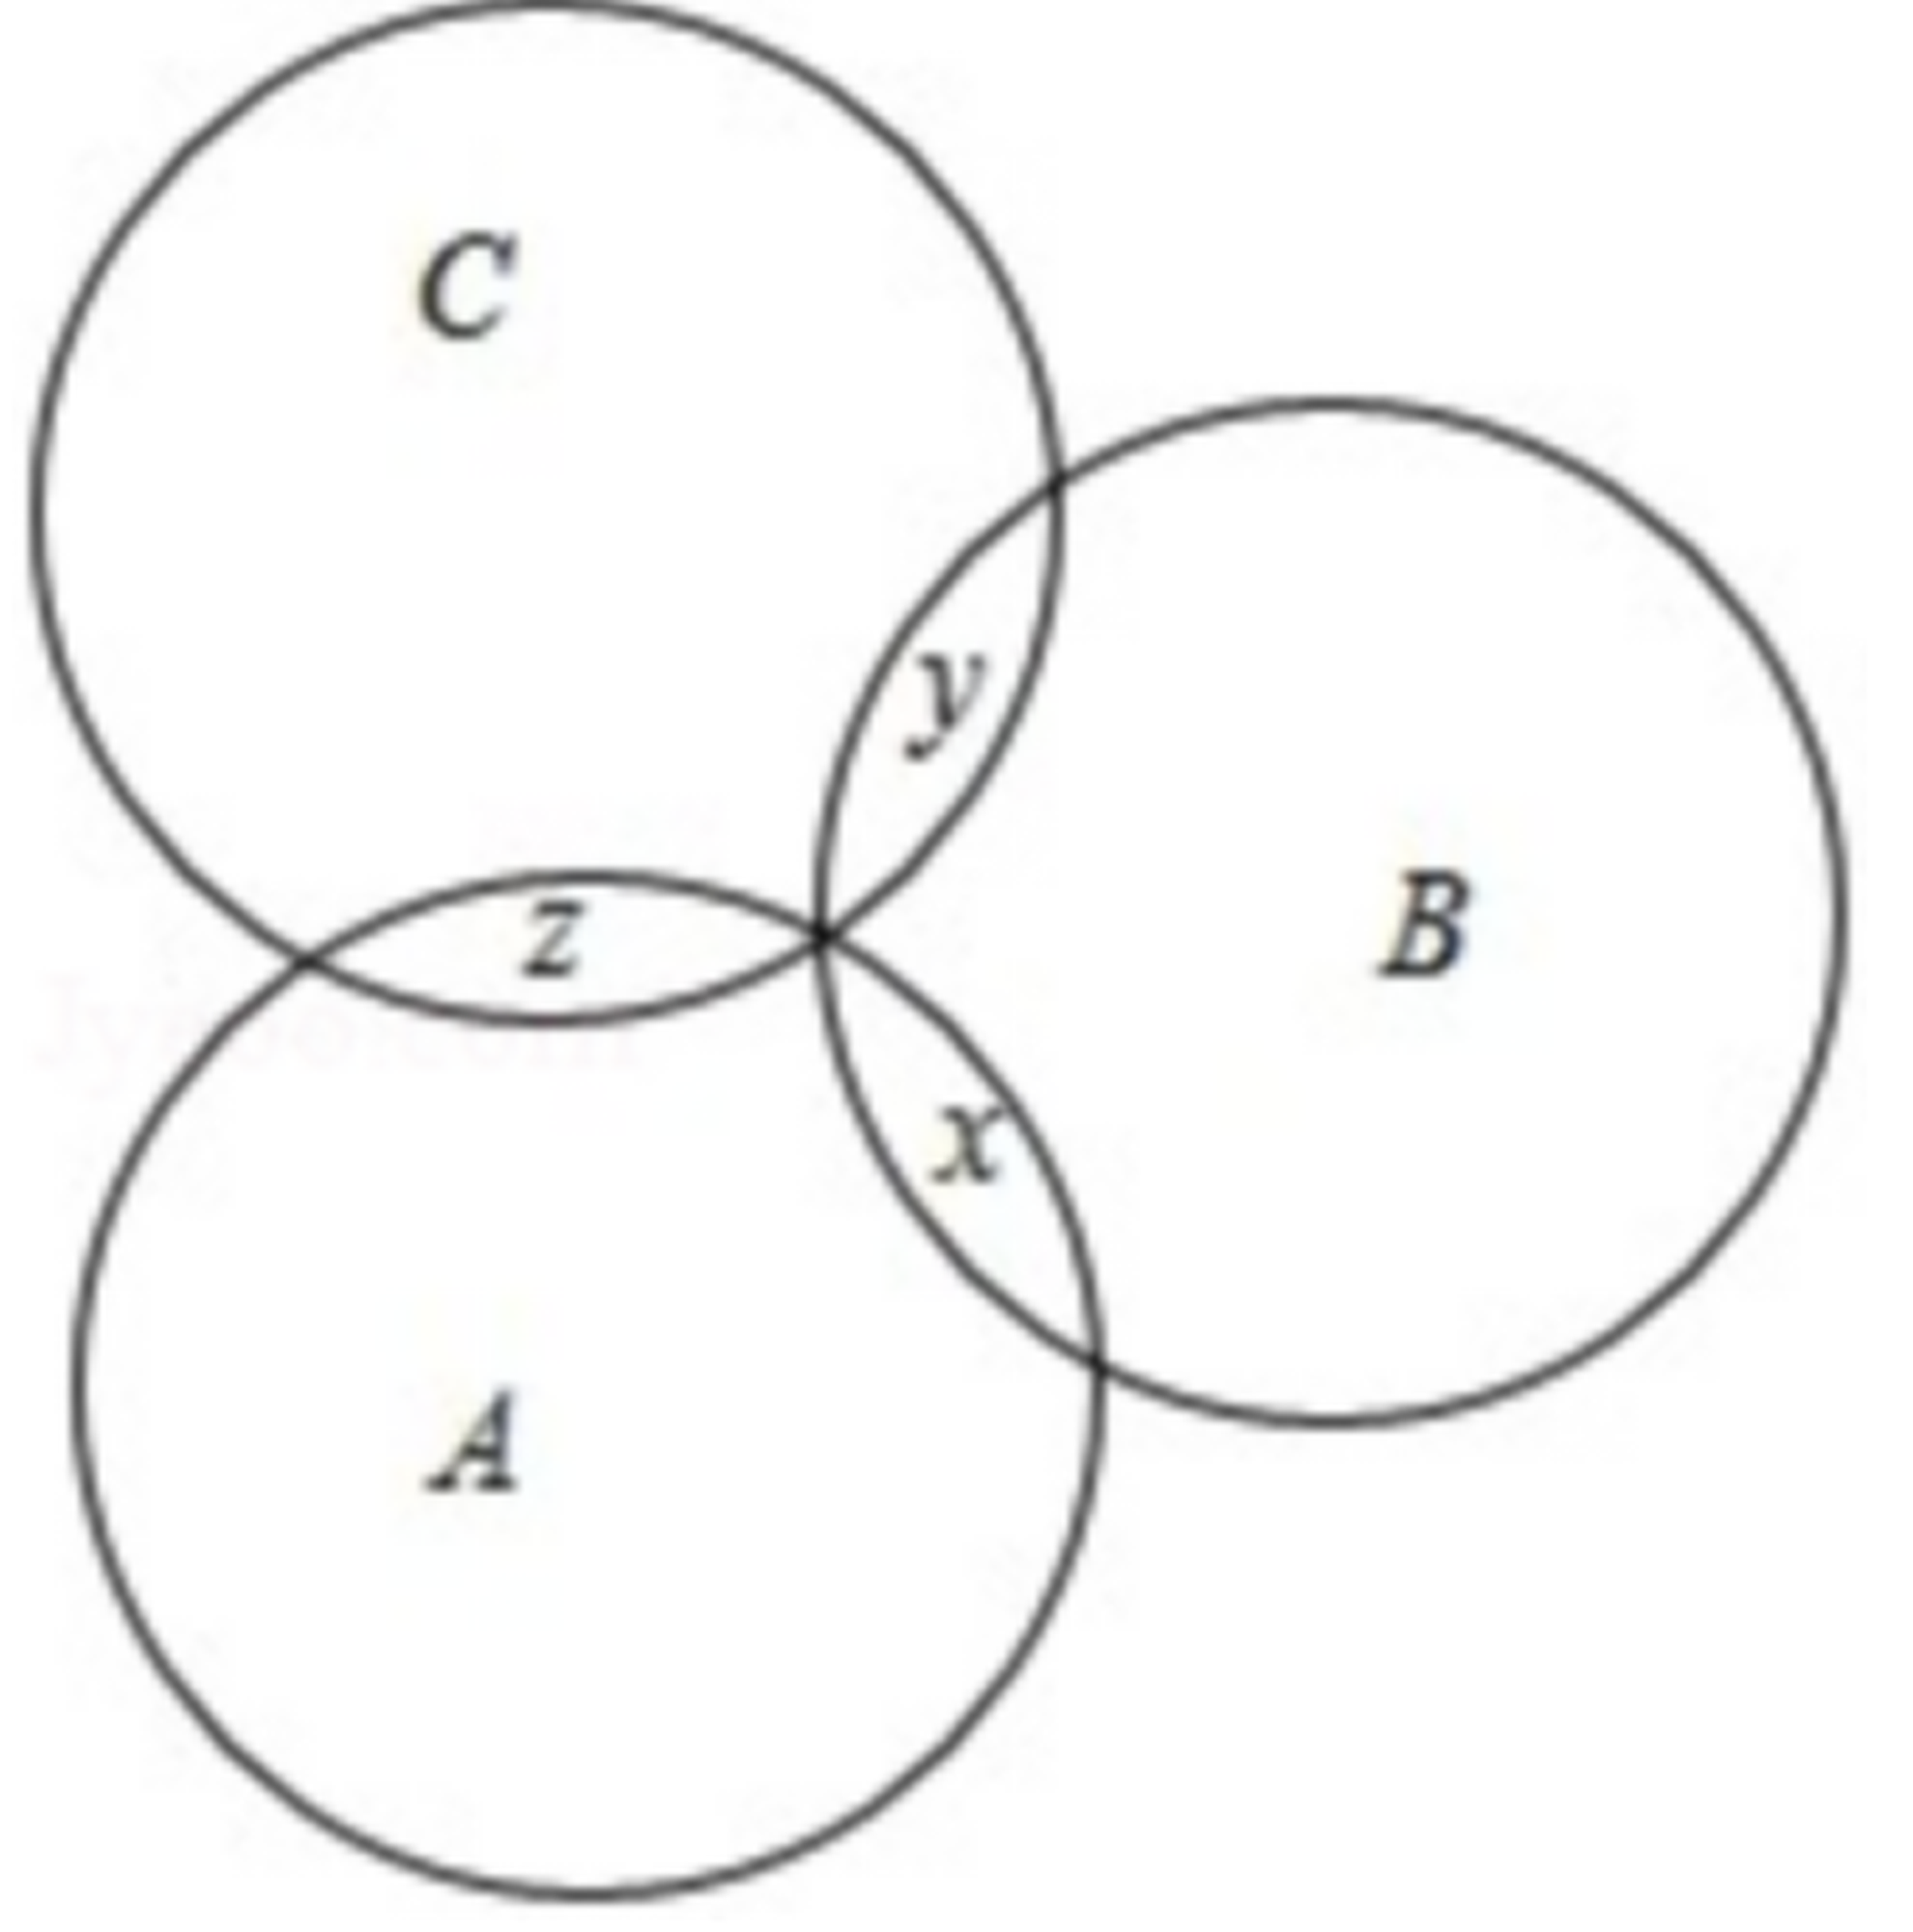
\includegraphics[width=0.30\textwidth]{figures/venn_ABC_x_y_z_h39.png}
\end{center}
\step{因为 $|A\cap B|=|B\cap C|=|C\cap A|=1$，且 $x$、$y$、$z\in\{1,2,3\}$，}
\step{所以集合 $A=\{x,z\}$，$B=\{x,y\}$，$C=\{z,y\}$，}
\step{若 $x=1$，$y=2$，$z=3$，则 $A=\{1,3\}$，$B=\{1,3\}$，$C=\{2,3\}$，}
\step{将 $1$，$2$，$3$ 进行全排列，有 $P_3^3=3\times2=6$ 个.}
\solend

\fi

\item 已知集合 $T=\{1,2,\cdots,2025\}$，对于 $T$ 的每一个非空子集的所有元素，计算它们乘积的倒数，
则所有这样倒数的和为 \blankline[4.4em].

\ans{$2025$}

\ifanswer
\solbegin
\step{集合 $T=\{1,2,\cdots,2025\}$ 的非空子集的个数为 $2^{2025}-1$，}
\step{这些子集中，每个元素的乘积分别为}
\step{$1,2,3,\cdots,2025,1\times2,1\times3,\cdots,1\times2025,\cdots,1\times2\times3\times\cdots\times2025$，}
\step{每项都可以看作是从 $1,2,3,\cdots,2025$ 中选择若干项的乘积，}
\step{$1+\dfrac12+\cdots+\dfrac{1}{2025}+\dfrac{1}{1\times2}+\dfrac{1}{1\times3}+\cdots+\dfrac{1}{2024\times2025}
+\cdots+\dfrac{1}{1\times2\times\cdots\times2025}$}
\step{$=(1+1)\left(1+\dfrac12\right)\cdots\left(1+\dfrac{1}{2025}\right)-1
=2\times\dfrac32\times\dfrac43\times\cdots\times\dfrac{2026}{2025}-1=2025$.}
\solend

\fi

% 第 24 题是压轴题，题干较长；试卷版在它之前量一次页高，尽量不与前文分家（照全稿成例）。
\ansneed{5cm}
% 注：原卷【解析】①③ 两步把 $f(x)$ 印作 $f[x[x]]$，显系笔误，照录未改，见文件头「笔误/存疑」⑦。
\item 若 $X$ 是一个集合，$T$ 是一个以 $X$ 的某些子集为元素的集合，且满足：①$X$ 属于 $T$，
$\varnothing$ 属于 $T$；②$T$ 中任意多个元素的并集属于 $T$；③$T$ 中任意多个元素的交集属于 $T$.
则称 $T$ 是集合 $X$ 上的一个拓扑. 已知函数 $f(x)=[x[x]]$，其中 $[x]$ 表示不大于 $x$ 的最大整数，
当 $x\in(0,n]$，$n\in\N^*$ 时，函数 $f(x)$ 值域为集合 $A_n$，则集合 $A_2$ 上的含有 $4$ 个元素的
拓扑 $T$ 的个数为 \blankline[4.4em].

\ans{$9$}

\ifanswer
\solbegin
\step{由题意，$n=2$，故 $0<x\leqslant2$，}
\step{①当 $0<x<1$ 时，则 $[x]=0$，所以 $f[x[x]]=0$，}
\step{②当 $x=1$ 时，$[x]=1$ 显然 $f(1)=1$，}
\step{③当 $1<x<2$ 时，$[x]=1$，所以 $f[x[x]]=[x]=1$，}
\step{④当 $x=2$ 时，$f(2)=4$，}
\step{所以 $A_2=\{0,1,4\}$，}
\step{因为 $T$ 中含有 $4$ 个元素，其中两个元素 $\varnothing$ 和 $A_2$，}
\step{$A_2=\{0,1,4\}$. 其它两个元素为 $A$、$B$，则
$\begin{cases}A\neq\varnothing\\ A\neq A_2\\ B\neq\varnothing\\ B\neq A_2\\ A\neq B\end{cases}$，}
\step{由对称性，不妨设 $1\leqslant|A|\leqslant|B|\leqslant2$，其中 $|A|$、$|B|$ 表示集合 $A$ 中元素的个数，}
\step{因为 $\begin{cases}A\cap B\in T\\ A\cup B\in T\end{cases}$，又 $|A|\leqslant|B|$，所以 $A\cap B=\varnothing$ 或 $A$，}
\step{若 $A\cap B=\varnothing$，则 $A\cup B$ 只能等于 $A_2$，}
\step{（若 $A\cup B=B$，则 $A\sub B$，则 $A\cap B=A=\varnothing$，矛盾）}
\step{则必有 $\begin{cases}|A|=1\\ |B|=2\end{cases}$，所以 $(A,B)$ 的个数 $\Leftrightarrow$ $A$ 的个数 $=3$ 种，}
\step{即 $\begin{cases}A=\{0\}\\ B=\{1,4\}\end{cases}$ 或 $\begin{cases}A=\{1\}\\ B=\{0,4\}\end{cases}$
或 $\begin{cases}A=\{4\}\\ B=\{0,1\}\end{cases}$；}
\step{若 $A\cap B=A\Leftrightarrow A\sub B$ 此时满足 $A\cup B=B$，}
\step{因为 $A\neq B$ 且 $1\leqslant|A|$ 且 $|B|\leqslant2$，所以 $\begin{cases}|A|=1\\ |B|=2\end{cases}$，}
\step{所以 $B$ 的选择共有 $C_3^2=3$ 种，则 $A$ 的个数有 $C_2^1$ 种，}
\step{所以 $(A,B)$ 的个数 $=2\times3=6$ 种.}
% 这六组「$A$／$B$」按原卷排作两行（前五个一行、第六个另起一行）；因五组并排时
% amsmath 的 cases 会为每组的第二列各留一枚 \quad，本行改排 \left\{\begin{matrix}…\end{matrix}\right.
% 以省下这枚 \quad（照 README「说明」记的高一07 成例），字形与 cases 相同。
\step{（这 $6$ 种是 $\left\{\begin{matrix}A=\{0\}\\ B=\{0,1\}\end{matrix}\right.$、
$\left\{\begin{matrix}A=\{1\}\\ B=\{0,1\}\end{matrix}\right.$、
$\left\{\begin{matrix}A=\{0\}\\ B=\{0,4\}\end{matrix}\right.$、
$\left\{\begin{matrix}A=\{4\}\\ B=\{0,4\}\end{matrix}\right.$、
$\left\{\begin{matrix}A=\{1\}\\ B=\{1,4\}\end{matrix}\right.$、}
\step{$\left\{\begin{matrix}A=\{4\}\\ B=\{1,4\}\end{matrix}\right.$）.}
\step{综上，$T$ 的个数为 $9$ 个.}
\solend

\fi

\end{enumerate}

\end{document}
"
%
% 原始材料是微信公众号图文（公众号「魔都数学加油站」连载「27学年高一 39」，署名「破晓」，
% 2026-09-26 21:29 发布，原文标题「27学年高一39——2026-2027年上海市大同中学高一上周末作业4.1」，
% 原文链接 https://mp.weixin.qq.com/s/HR2hIayXUXNi4zTs3PioiQ ），正文为 11 张 PNG 页。**同一篇里各页分辨率不一致**（2560×3620 与 4762×6735 两档混排：第 1、3、8、10 页为
% 2560×3620，第 2、4、5、6、7、9、11 页为 4762×6735）。原文本身就是一份**讲评版**——除第 15 题
% 外各题题下直接印【解析】（无单独的【答案】行），第 15 题的答案「D」直接印在题干末尾的括号内。
% 试题文字、答案与解析均照原卷录入，未改内容。卷面的粉色斜水印「魔都数学加油站」属水印，未录入。
%
% 卷首标题：原卷页首印作「2026-2027 年大同中学高一上周末作业 4.1」（**卷面标题行即带校名**，
% 年份区间按全稿惯例排 en dash，前缀照原卷保留「年」）。
%
% 篇幅与题号：卷面自「一、填空题」的**第 3 题**起编，终于「附加题」的**第 24 题**，共 22 题
% （填空 3—12、选择 13—16、解答 17—20、附加题 21—24）。第 1、2 题未在该文中发布——这是该
% 公众号连载讲评版的通例（高一02—高一09 等均自第 3 题起编，README「说明」已记），**不是截断**，
% 故本稿题号亦自 3 起。它与 高一40（大同中学 周末作业4.2）同属「周末作业 4」系列但**各自独立起编**
% （4.2 自第 3 题起、终于第 19 题），不是同一份试卷的两半。
%
% 与原卷的排版差异（均已在 README「说明」中交代）：
%   ① 原文自**第 3 题**起（第 1、2 题未在该文中发布），故本稿题号亦自 3 起，填空题以
%      \setcounter{enumi}{2} 起编；选择、解答、附加题三节各按上一节末号另设 \setcounter
%      （选择题 \setcounter{enumi}{12}、解答题 \setcounter{enumi}{16}、附加题 \setcounter{enumi}{20}）；
%   ② 原卷本就印有「一、填空题」「二、选择题」「三、解答题」三节标题，末节印作「附加题」
%      （**不带「四、」**，且题号 21—24 续前编、不另起），本稿照原卷分节，只把标题改排成全稿
%      统一的「大节标题」样式；
%   ③ 原卷是「讲评版」：除第 15 题外，各题题下均印【解析】（**全卷无一条独立的【答案】行**）；
%      第 15 题无解析，答案「D」直接印在题干末尾的括号内。本稿统一改为试卷版隐去、答案版以
%      \ans{}／\ifanswer 块给出，两版彻底分离；原卷写在【解析】末句的结果，本稿照 高一38
%      （同校同系列、同为讲评版）的成例另提为 \ans{}；
%   ④ 数集记号原卷两套并用：实数集作斜体的 $R$（第 7、11、14、17、18、19 题），整数集作斜体
%      $Z$（第 10 题），自然数集作斜体 $N$ 及 $N^*$（第 16、20、21、24 题），本稿按全稿惯例
%      统一写作 $\R$、$\Z$、$\N$、$\N^*$；
%   ⑤ 补集符号原卷两套并用：第 7 题作前缀式的 $C_U$（且题干称全集为 $I$，见「笔误/存疑」①），
%      第 14、15、18 题作上横线（$\overline{H}$、$\overline{A}$、$\overline{B}$），本稿照录、不归一
%      （前缀式写作 $\complement_U$，与 高一c／高一10 的成例一致）；
%   ⑥ 包含符号原卷两套并用：第 3 题作**无下划线**的 $\subset$，第 15、18、20、24 题作**带下划线**
%      的 $\sub$，本稿照录、不归一；
%   ⑦ 原卷填空的横线约两个字宽，本稿按全稿惯例统一排 \blankline[4.4em]；
%   ⑧ 第 7、11、22 题各有插图，取原卷截图、4× LANCZOS 放大（figures/venn_N_cap_CI_M_h39.png、
%      figures/plane_grid_4squares_h39.png、figures/venn_ABC_x_y_z_h39.png）；第 7 题的 Venn 属
%      **题干**（试卷版、答案版都出），第 11、22 题的图在【解析】内（仅答案版出）。第 7 题图
%      左下、第 11 题图的上／左／右边缘带进极淡的原卷粉色水印残影——照全稿「插图直接取自
%      原卷截图、不用 TikZ 重绘、不修图」的体例保留（再裁会切到坐标轴与 $x$、$y$、$O$ 标注）；
%   ⑨ 原卷并列的字母、数字（「$x_1,x_2$」「$a,b$」「$1,2,3,\cdots,11$」）多作半角逗号或不加标点，
%      本稿按全稿惯例改排顿号（$x_1$、$x_2$）或把数列并入行内公式；半角括号、逗号一律排全角，
%      数学式内部的标点照原样；
%   ⑩ 原卷未印副标题，本稿按**本卷实际内容**补出副标题「集合与常用逻辑用语」（依据见下条）。
%
% 副标题（\examtitlest 第二个参数）：本卷卷面未印副标题，由本稿补出，取值按 2026-09-26 起的
%   新口径「只用本卷实际内容的模块名」定为「集合与常用逻辑用语」。依据：全卷 22 题（第 3—24 题）中，
%   第 3、5、7、8、10、11、14、15、16、17、18、19、20、21、22、23、24 题共 17 题是集合的运算与
%   关系、子集／真子集、补集、集合新定义（「全食／偏食」、最小相交、拓扑、特征数）与集合计数，
%   以及命题与常用逻辑用语（第 3 题充要条件、第 5 题存在量词命题、第 17 题命题真假）；其余两题
%   第 4、6 考一元二次方程的根（韦达定理）与方程恒等，第 9、12、13 题是不等式（一元二次不等式组
%   的整数解、一元二次不等式解集、不等式的性质）——不等式合计 3/22，**不足全卷三分之一**，
%   故不并标「不等式」。
%
% 原卷笔误/存疑（均照抄原卷、未改，见源码中该处上方注释）：
%   ① 第 7 题题干称「全集 $I=R$」，而【解析】两处把补集写作 $C_U M$（下标作 $U$），前后记号不一；
%      本稿照录，未改；
%   ② 第 4 题【解析】两处把判别式印作 $\triangle=[2(m-1)^2-16m^2]$（方括号内首项漏了平方，
%      正确应作 $[2(m-1)]^2-16m^2$）；按其所判「$m=\frac12$ 时 $<0$、$m=-\frac12$ 时 $>0$」反推，
%      $[2(m-1)]^2-16m^2$ 在 $m=\frac12$ 时为 $-3<0$、在 $m=-\frac12$ 时为 $5>0$，与结论一致；
%      本稿照录；
%   ③ 第 9 题【解析】把方程组第二式印作 $1-2<-k\leqslant3$，按其结论 $-3\leqslant k<2$ 反推，
%      疑当作 $-2<-k\leqslant3$（原卷多一个「$1$」）；本稿照录；
%   ④ 第 17 题【解析】首句「由数 $y=-x^2+ax-1=-x+3$」中的「由数」显系「由」或「由函数」之误；
%      且末段「若 $p$ 真 $q$ 假…得 $a\in R$」「若 $p$ 假 $q$ 真…此时 $a$ 无解」与结论「$a$ 的取值范围
%      是 $R$」自相矛盾（按 $p:a\leqslant-5$、$q:a>-6$，$p$ 真 $q$ 假应为 $a\leqslant-6$，$p$ 假 $q$ 真
%      应为 $a>-5$，合起来是 $a\leqslant-6$ 或 $a>-5$，并非 $R$）；本稿一律照录，未按正确解法改写；
%   ⑤ 第 18 题【解析】(2) 把 $B=\{x\mid x^2+a\leqslant0\}$（$a<0$）印作右端开的
%      $\{x\mid-\sqrt{-a}\leqslant x<\sqrt{-a}\}$（应为闭的「$\leqslant$」）；按其所判
%      $\sqrt{-a}<\frac12$ 反推，不影响结论；本稿照录；
%   ⑥ 第 22 题【解析】在 $x=1$、$y=2$、$z=3$ 时把 $B=\{x,y\}$ 印作 $\{1,3\}$（应为 $\{1,2\}$），
%      与本行前面「$B=\{x,y\}$」不合；本稿照录；
%   ⑦ 第 24 题【解析】①③ 两步把 $f(x)$ 印作 $f[x[x]]$，显系笔误；本稿照录。
%   ⑧ 第 8 题【解析】「即方程 $x^2+ax+b=x$，$x^2+(a-1)x+b=0$ **由**两个相等的实数根为 $4$」——
%      「由」当为「有」（「设…是…有」的杂糅）；本稿照录；
%   ⑨ 第 10 题：题设 $a\oplus b=b(a^2+b^2+1)$，而集合定义里含 $\dfrac{a\oplus b}{2b}$；$-2<a<b<2$、
%      $a$、$b\in\Z$ 时 $(a,b)=(-1,0)$ 也合条件、却使分母 $2b=0$，原卷解析仍代入该组并约去
%      $b$ 得 $x=1$（答案集恰好不变）；本稿照录；
%   ⑩ 第 15 题选项列里 ② 与 ③ 之间**漏排分隔号**（原卷作「② $\overline{A}\cap B=\varnothing$③
%      $\overline{A}\sub\overline{B}$；」——①、③ 后都有「；」，② 后没有）；本稿照录；
%   ⑪ 第 20(2) 把 $\{1,2,\cdots,20\}$ 分成的 11 个集合里，$\{8,11\}$ 与 $\{9,12\}$ 之间误用
%      **句号**「.」（同行其余处皆逗号）；本稿照录；
%   ⑫ 第 20(3)① 推理不严：原卷写「选 5 则不选 1、9；选 6 则不选 2、10；选 7 则不选 3、11；
%      则只剩 4、8」——但 4 与 8 相差 $4$、不能同选，该情形实际最多只能取 $4$ 个；末句结论
%      「不超过 $5$ 个」仍成立；本稿照录；
%   ⑬ 第 16 题【解析】两种下标并存：「所以在 $A_i$ 的特征数构成中」原卷作斜体 $A_i$，而
%      「要使 $X_1+X_2+X_3$ 最大（小），则（应）在集合 $A_1$ 中首先放置…」两处原卷作
%      **数字 $1$**（与同句 $X_1$ 的角标同形）；本稿照录、未归一。
%
% 图取原卷截图（依次见各处的 \includegraphics 前的注释），4× LANCZOS 放大。
\documentclass[a4paper,11pt]{article}
\usepackage{common}

\begin{document}

\examtitlest[3]{2026--2027 年大同中学高一上周末作业 4.1}{集合与常用逻辑用语}

\bigsec{一、填空题}

\begin{enumerate}
\setcounter{enumi}{2}

\item “$x\geqslant a$”是“$0<x<2$”的必要非充分条件，则实数 $a$ 的取值范围是 \blankline[4.4em].

\ans{$(-\infty,0]$}

\ifanswer
\solbegin
\step{因为 $x\geqslant a$ 是 $0<x<2$ 的必要非充分条件，所以 $(0,2)\subset[a,+\infty)$，所以 $a\leqslant0$，}
\step{则实数 $a$ 的取值范围是 $(-\infty,0]$.}
\solend

\fi

% 注：原卷$[2(m-1)^2-16m^2]$ 首项漏了平方（应为 $[2(m-1)]^2-16m^2$），照录未改，见文件头「笔误/存疑」②。
\item 若关于 $x$ 的方程 $x^2+2(m-1)x+4m^2=0$ 有两个实数根，且这两根互为倒数，则 $m=$ \blankline[4.4em].

\ans{$-\dfrac12$}

\ifanswer
\solbegin
\step{设 $x_1$、$x_2$ 是方程 $x^2+2(m-1)x+4m^2=0$ 有两个实数根，}
\step{则 $x_1x_2=4m^2=1$，解得 $m=\dfrac12$ 或 $m=-\dfrac12$，}
\step{又当 $m=\dfrac12$ 时，$\triangle=[2(m-1)^2-16m^2]<0$，舍去，}
\step{当 $m=-\dfrac12$ 时，$\triangle=[2(m-1)^2-16m^2]>0$，故 $m=-\dfrac12$.}
\solend

\fi

\item 已知命题：“存在 $x\in[1,2]$，使 $x^2+2x+a\geqslant0$”为真命题，则 $a$ 的取值范围是 \blankline[4.4em].

\ans{$a\geqslant-8$}

\ifanswer
\solbegin
\step{若存在 $x\in[1,2]$，使 $x^2+2x+a\geqslant0$，}
\step{则等价为存在 $x\in[1,2]$，使 $x^2+2x\geqslant-a$，}
\step{当存在 $x\in[1,2]$ 时，设 $y=x^2+2x=(x+1)^2-1$，则 $3\leqslant y\leqslant8$，}
\step{所以要使 $x^2+2x\geqslant-a$，则 $8\geqslant-a$，即 $a\geqslant-8$.}
\solend

\fi

\item 已知方程 $a(3x+2)+b(2x-3)=8x+3$ 有无穷多个解，则 $a:b=$ \blankline[4.4em].

\ans{$30:7$}

\ifanswer
\solbegin
\step{$a(3x+2)+b(2x-3)=(3a+2b)x+2a-3b=8x+3$ 有无穷多个解，}
\step{所以 $\begin{cases}3a+2b=8\\ 2a-3b=3\end{cases}$，解得 $a=\dfrac{30}{13}$，$b=\dfrac{7}{13}$，所以 $a:b=30:7$.}
\solend

\fi

% 注：原卷题干称「全集 $I=R$」，而【解析】两处把补集写作 $C_U M$（下标作 $U$），前后记号不一；
%     照录未改，见文件头「笔误/存疑」①。
\item 已知集合 $M=\{x\mid y=\sqrt{3-x^2}\}$，$N=\{x\mid-3\leqslant x\leqslant1\}$，全集 $I=\R$，
则图中阴影部分表示的集合为 \blankline[4.4em].

% 图取原卷截图（01.png，2560×3620）右栏，4× LANCZOS 放大。
\begin{center}
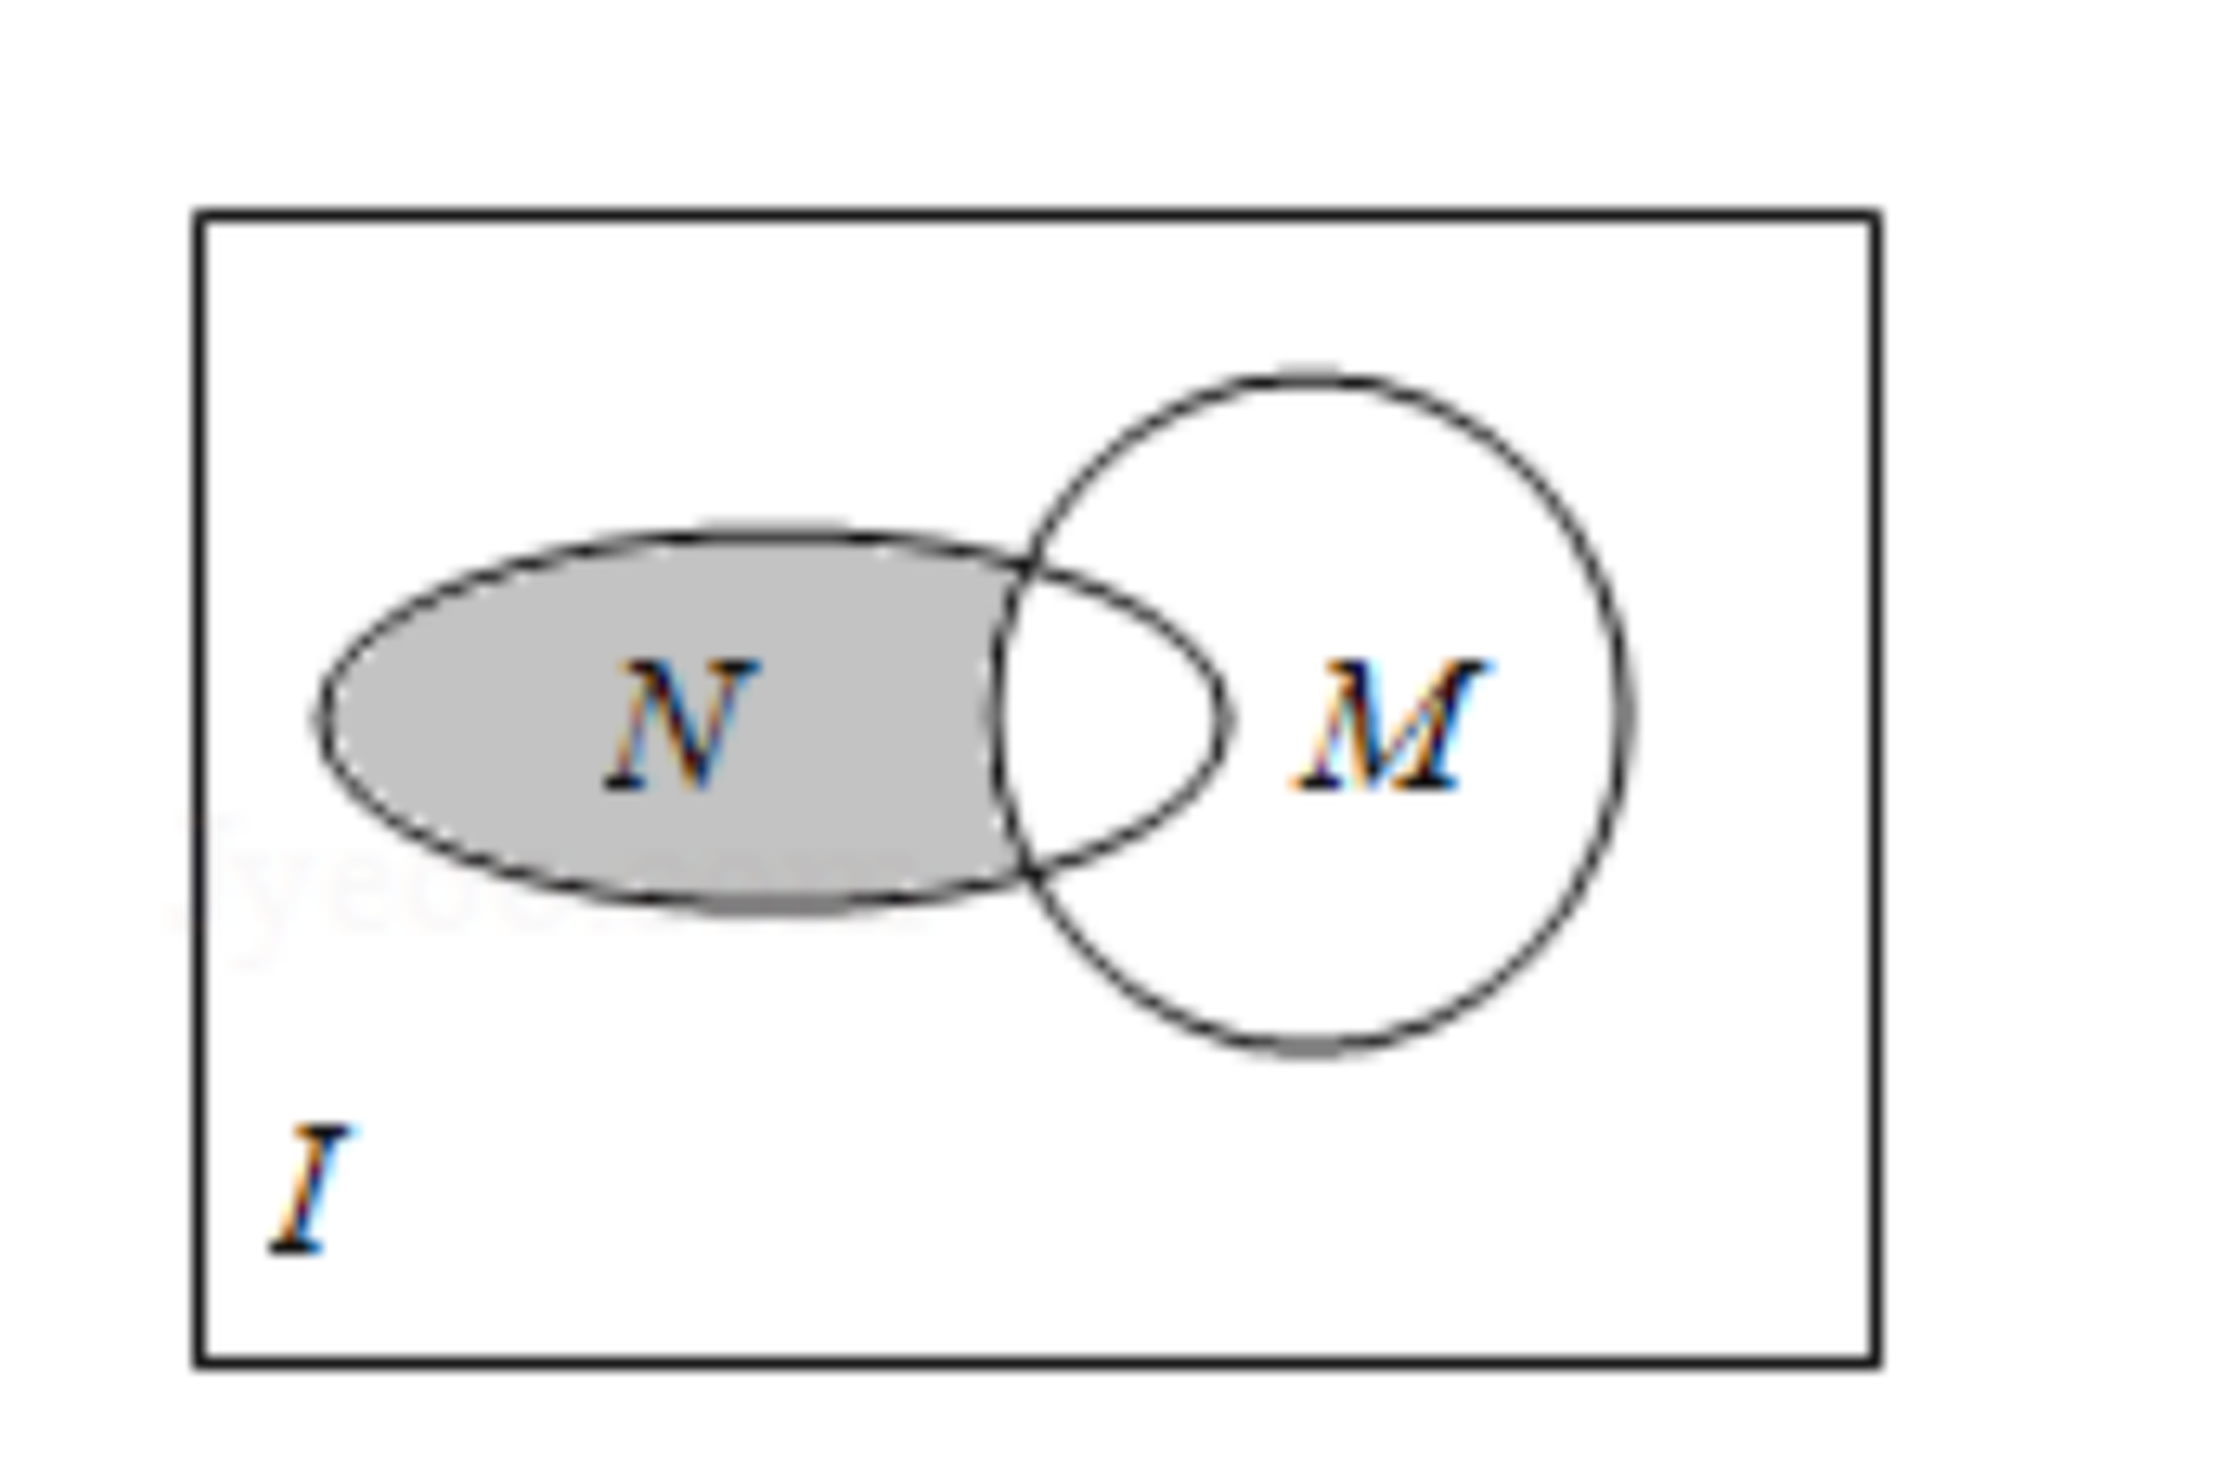
\includegraphics[width=0.30\textwidth]{figures/venn_N_cap_CI_M_h39.png}
\end{center}

\ans{$[-3,-\sqrt3)$}

\ifanswer
\solbegin
\step{阴影部分用集合表示为 $N\cap(\complement_UM)$.}
\step{则 $M=\{x\mid y=\sqrt{3-x^2}\}=\{x\mid3-x^2\geqslant0\}=\{x\mid-\sqrt3\leqslant x\leqslant\sqrt3\}$，}
\step{则 $\complement_UM=\{x\mid x>\sqrt3\text{ 或 }x<-\sqrt3\}$，$N=\{x\mid|x+1|\leqslant2\}=\{x\mid-3\leqslant x\leqslant1\}$，}
\step{则 $N\cap(\complement_UM)=\{x\mid-3\leqslant x<-\sqrt3\}$.}
\solend

\fi

\item 已知 $f(x)=x^2+ax+b$，集合 $\{x\mid f(x)=x\}=\{4\}$，将集合 $M=\{x\mid f(x)=4\}$ 用列举法表示 \blankline[4.4em].

\ans{$\{3,4\}$}

\ifanswer
\solbegin
\step{已知 $f(x)=x^2+ax+b$，集合 $\{x\mid f(x)=x\}=\{4\}$，}
% 注：原卷本行作「…$x^2+(a-1)x+b=0$ **由**两个相等的实数根为 $4$」——「由」当为「有」
%     （「设…是…有」的杂糅）；本稿照录未改，见文件头「原卷笔误/存疑」⑧。
\step{即方程 $x^2+ax+b=x$，$x^2+(a-1)x+b=0$ 由两个相等的实数根为 $4$，}
\step{所以 $\triangle=(a-1)^2-4b=0$，即 $x^2+(a-1)x+b=(x-4)^2$，所以 $b=16$，$a=-7$，}
\step{所以 $f(x)=x^2+ax+b=x^2-7x+16$，所以集合 $M=\{x\mid f(x)=4\}$，}
\step{即 $x^2-7x+16=4$，$x^2-7x+12=0$，故 $M=\{x\mid f(x)=4\}=\{3,4\}$.}
\solend

\fi

% 注：原卷方程组第二式印作 $1-2<-k\leqslant3$，按其结论 $-3\leqslant k<2$ 反推疑当作 $-2<-k\leqslant3$，
%     照录未改，见文件头「笔误/存疑」③。
\item 关于 $x$ 的不等式组 $\begin{cases}x^2-x-2>0\\ 2x^2+(2k+5)x+5k<0\end{cases}$ 的整数解的集合为 $\{-2\}$，
则实数 $k$ 的取值范围 \blankline[4.4em].

\ans{$-3\leqslant k<2$}

\ifanswer
\solbegin
\step{原不等式组即 $\begin{cases}(x-2)(x+1)>0\\ (x+k)(2x+5)<0\end{cases}$，整数解的集合为 $A$，若 $A=\{-2\}$，}
\step{则 $(-2+k)(2\times(-2)+5)<0$，所以 $k<2$，且有 $\begin{cases}-k>-\dfrac52\\ 1-2<-k\leqslant3\end{cases}$，}
\step{解得 $-3\leqslant k<2$.}
\solend

\fi

\item 规定 $\oplus$ 与 $\otimes$ 是两个运算符号，其运算法则如下，对任意实数 $a$、$b$ 有：$a\otimes b=ab$，
$a\oplus b=b(a^2+b^2+1)$. 若 $-2<a<b<2$ 且 $a$、$b\in\Z$，
$A=\left\{x\mid x=2(a\otimes b)+\dfrac{a\oplus b}{2b}\right\}$，则用列举法表示集合 $A=$ \blankline[4.4em].

\ans{$\left\{1,-\dfrac12\right\}$}

\ifanswer
\solbegin
\step{$A=\left\{x\mid x=2(a\otimes b)+\dfrac{a\oplus b}{2b}\right\}
=\left\{x\mid x=2ab+\dfrac{b(a^2+b^2+1)}{2b}\right\}$}
\step{$=\left\{x\mid x=2ab+\dfrac12a^2+\dfrac12b^2+\dfrac12\right\}
=\left\{x\mid x=\dfrac12(a+b)^2+ab+\dfrac12\right\}$，}
% 注：题设含 $\dfrac{a\oplus b}{2b}$，而 $-2<a<b<2$、$a$、$b\in\Z$ 时 $(a,b)=(-1,0)$ 也合条件、
%     却使分母 $2b=0$；原卷解析仍代入该组并约去 $b$ 得 $x=1$（答案集恰好不变）。本稿照录，
%     见文件头「原卷笔误/存疑」⑨。
\step{当 $a=-1$，$b=0$ 时，$x=1$；当 $a=-1$，$b=1$ 时，$x=-\dfrac12$；}
\step{当 $a=0$，$b=1$ 时，$x=1$；所以 $A=\left\{1,-\dfrac12\right\}$.}
\solend

\fi

\item 高斯是德国著名的数学家，近代数学奠基者之一，享有“数学王子”的称号，为了纪念数学家高斯，
我们把取整函数 $y=[x]$，$x\in\R$ 称为高斯函数，其中 $[x]$ 表示不超过 $x$ 的最大整数，
如 $[1.1]=1$，$[-1.1]=-2$. 则点集 $P=\{(x,y)\mid[x]^2+[y]^2=1\}$
所表示的平面区域的面积是 \blankline[4.4em].

\ans{$4$}

\ifanswer
\solbegin
\step{$[x]^2+[y]^2=1$ 由 $\begin{cases}[x]=0\\ [y]=-1\end{cases}$ 或 $\begin{cases}[x]=0\\ [y]=1\end{cases}$
或 $\begin{cases}[x]=-1\\ [y]=0\end{cases}$ 或 $\begin{cases}[x]=1\\ [y]=0\end{cases}$ 四个平面区域组成，}
\step{即 $\begin{cases}0\leqslant x<1\\ -1\leqslant y<0\end{cases}$ 或 $\begin{cases}0\leqslant x<1\\ 1\leqslant y<2\end{cases}$
或 $\begin{cases}-1\leqslant x<0\\ 0\leqslant y<1\end{cases}$ 或 $\begin{cases}1\leqslant x<2\\ 0\leqslant y<1\end{cases}$，}
\step{作出平面区域如图所示，平面区域由四个边长为 $1$ 的正方形组成，}
% 图在【解析】内（仅答案版出），取原卷截图（03.png，2560×3620）中部，4× LANCZOS 放大。
\begin{center}
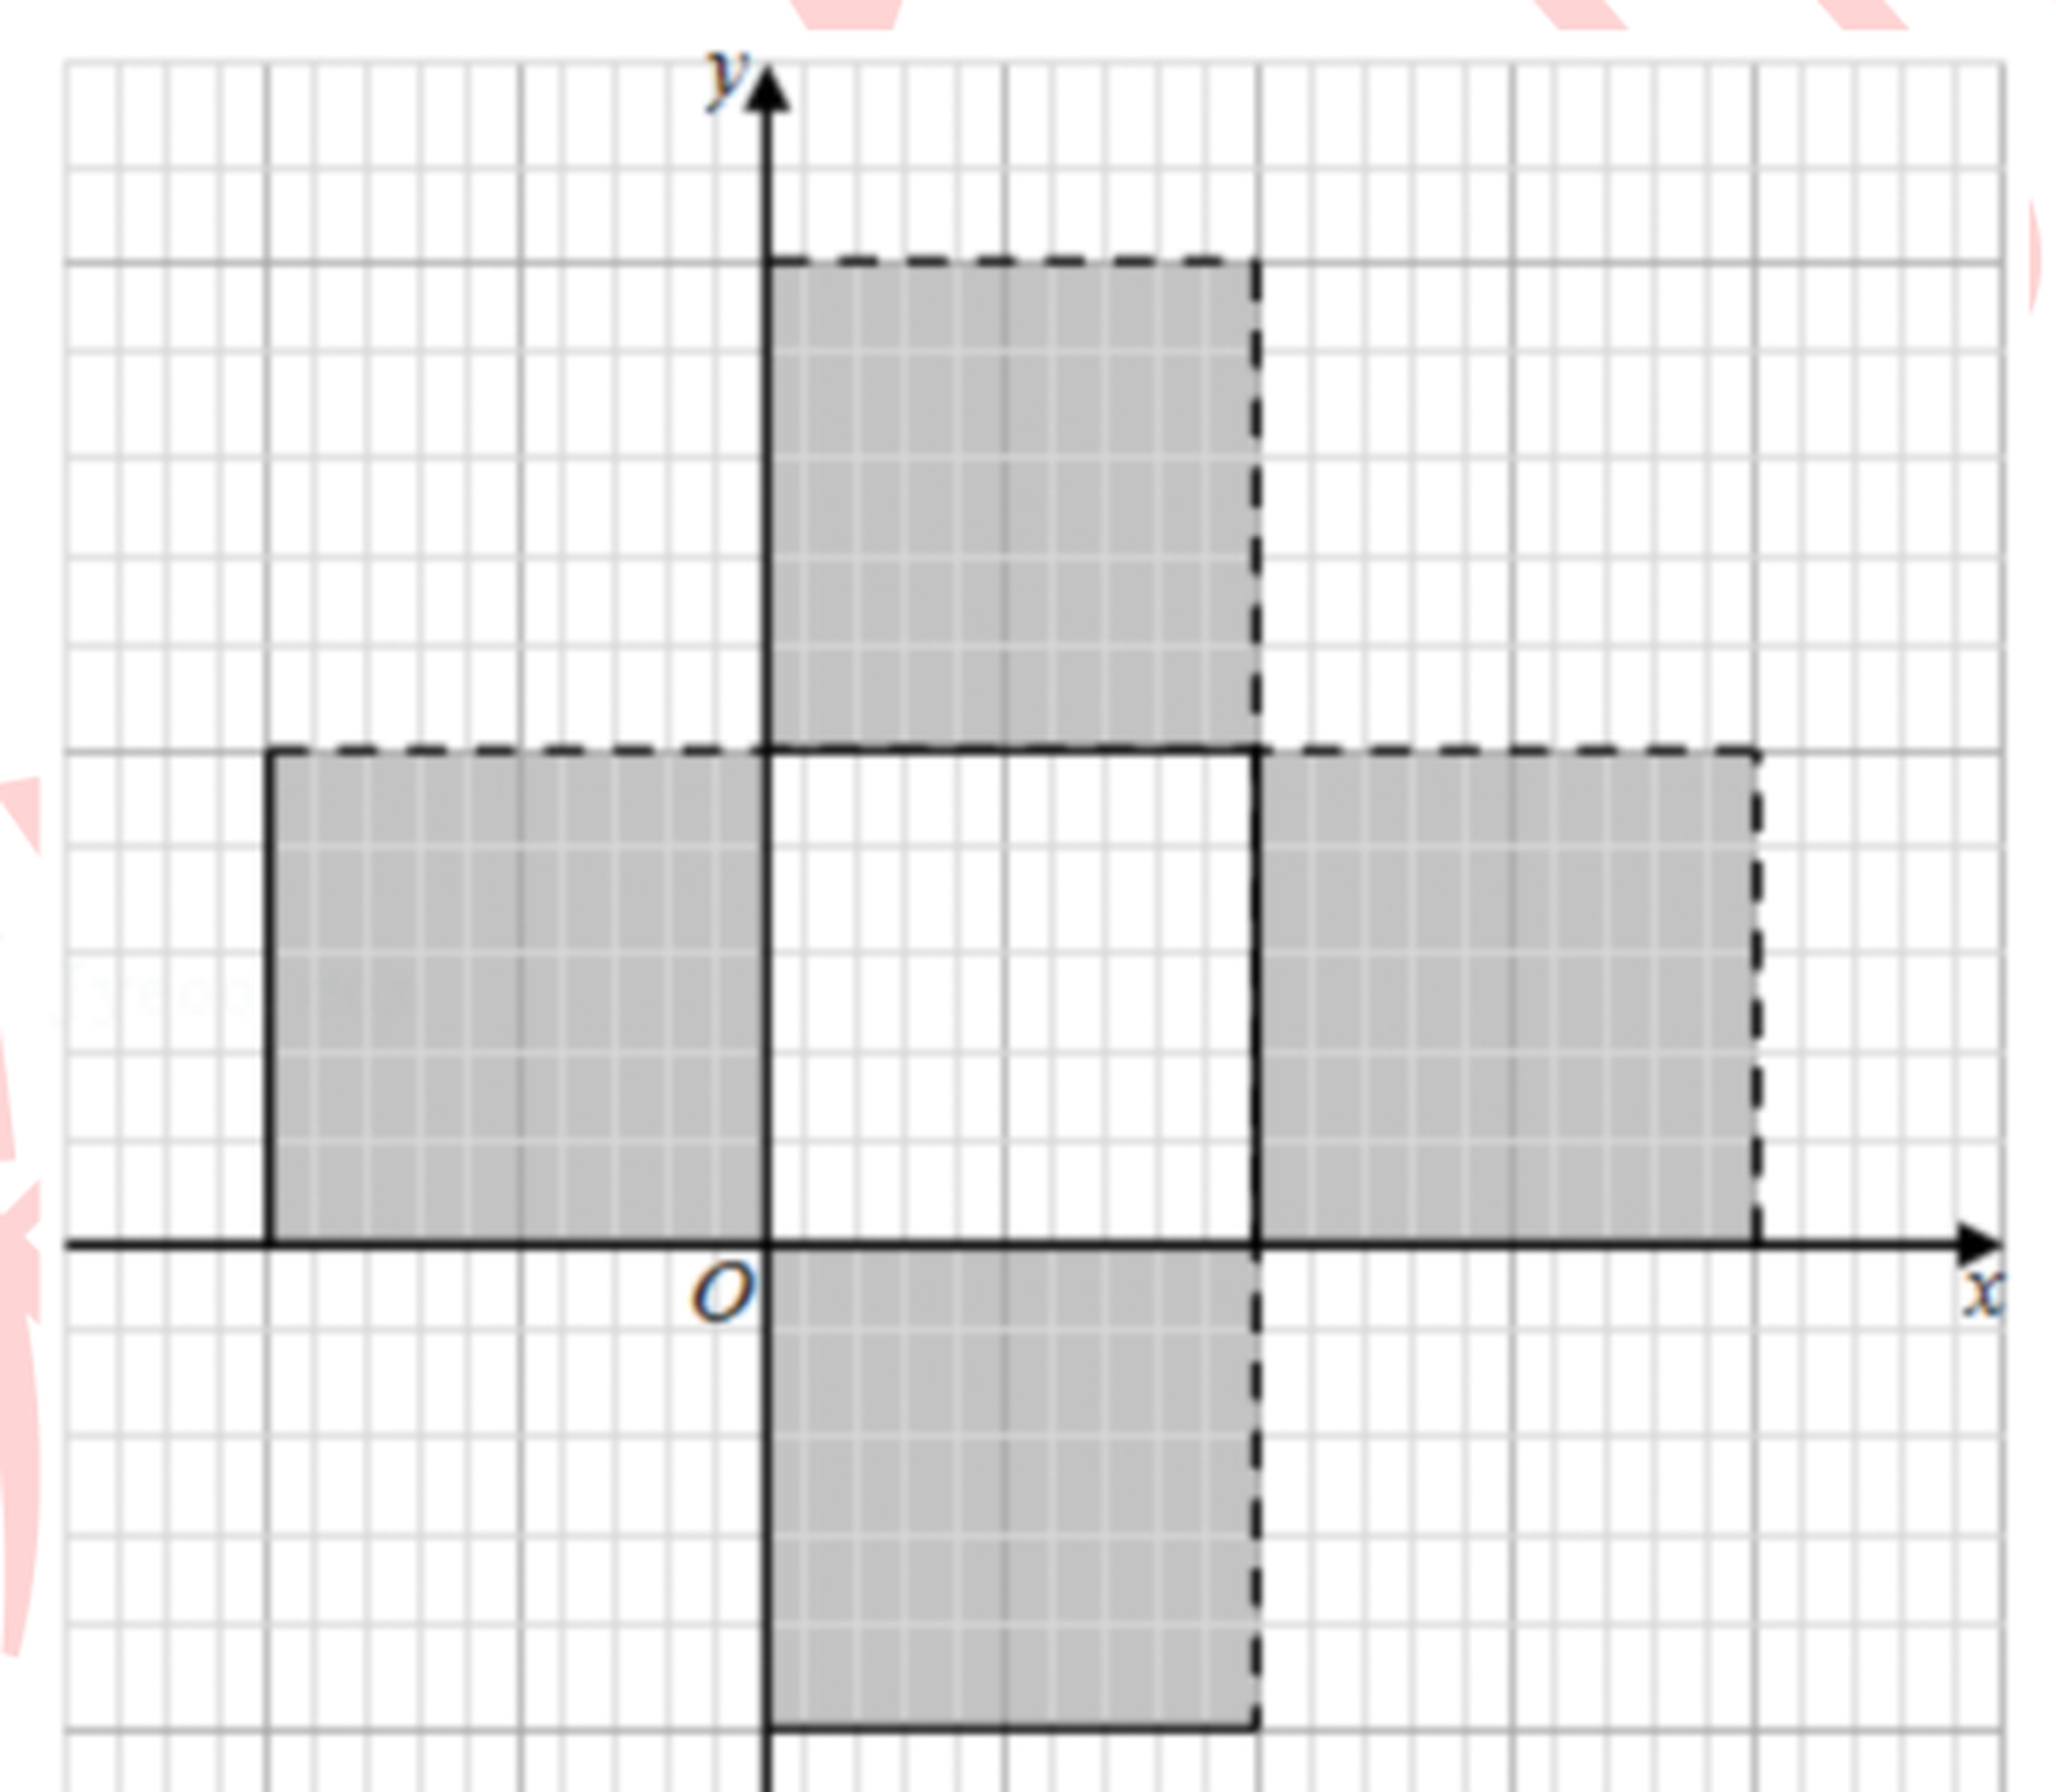
\includegraphics[width=0.38\textwidth]{figures/plane_grid_4squares_h39.png}
\end{center}
\step{总面积为 $1\times4=4$.}
\solend

\fi

\item 关于 $x$ 的不等式 $ax^2+bx+c>0$ 的解集为 $\{x\mid x<\beta\text{ 或 }x>\gamma\}(0<\beta<\gamma)$，
则不等式 $a(x^2+1)+b(x-1)+c>2ax$ 的解集为 \blankline[4.4em].

\ans{$(-\infty,\beta+1)\cup(\gamma+1,+\infty)$}

\ifanswer
\solbegin
\step{由题意得 $\beta$、$\gamma$ 为方程 $ax^2+bx+c=0$ 的两根且 $a>0$，}
\step{则 $\beta+\gamma=-\dfrac ba$，$\beta\gamma=\dfrac ca$，故 $b=-a(\beta+\gamma)$，$c=\beta\gamma a$，}
\step{则不等式可化为 $a(x^2+1)-a(\beta+\gamma)(x-1)+\beta\gamma a>2ax$，}
\step{因为 $a>0$，所以 $x^2+1-(\beta+\gamma)(x-1)+\beta\gamma>2x$，}
\step{即 $x^2-(\beta+\gamma+2)x+(\beta+\gamma+\beta\gamma+1)>0$，所以 $(x-\beta-1)(x-\gamma-1)>0$，}
\step{解得 $x<\beta+1$ 或 $x>\gamma+1$，所以不等式解集为 $(-\infty,\beta+1)\cup(\gamma+1,+\infty)$.}
\solend

\fi

\end{enumerate}

\bigsec{二、选择题}

\begin{enumerate}
\setcounter{enumi}{12}

\item 设 $a<b<0$，则下列不等式中不成立的是\mbox{（\quad）}

\keepwithprev
A. $\dfrac1a>\dfrac1b$\qquad B. $\dfrac{1}{a-b}>\dfrac1a$\qquad C. $|a|>-b$\qquad D. $\sqrt{-a}>\sqrt{-b}$

\ans{$B$}

\ifanswer
\solbegin
\step{令 $a=-2$，$b=-1$，}
\step{A、$-\dfrac12>-1$，正确；B、$-1<-\dfrac12$，故 B 错误；C、$2>1$，正确；}
\step{D、$\sqrt2>1$，正确；故选 B.}
\solend

\fi

\item 设实数集 $\R$ 为全集，集合 $P=\{x\mid f(x)=0\}$，$Q=\{x\mid g(x)=0\}$，$H=\{x\mid h(x)=0\}$，
则方程 $\dfrac{f^2(x)+g^2(x)}{h(x)}=0$ 的解集是\mbox{（\quad）}

\keepwithprev
A. $P\cap Q\cap\overline{H}$\qquad B. $P\cap Q$\qquad C. $P\cap Q\cap H$\qquad D. $P\cap Q\cup H$

\ans{$A$}

\ifanswer
\solbegin
\step{方程 $\dfrac{f^2(x)+g^2(x)}{h(x)}=0$ 等价于 $\begin{cases}f(x)=0\\ g(x)=0\\ h(x)\neq0\end{cases}$，}
\step{又因为 $P=\{x\mid f(x)=0\}$，$Q=\{x\mid g(x)=0\}$，$H=\{x\mid h(x)=0\}$，}
\step{所以方程 $\dfrac{f^2(x)+g^2(x)}{h(x)}=0$ 的解集是 $P\cap Q\cap\overline{H}$，故选 A.}
\solend

\fi

\item 设全集 $U$，在下列条件中，是 $B\sub A$ 的充要条件的有\mbox{（\quad）}

\keepwithprev
% 注：原卷此行 ② 与 ③ 之间**漏排分隔号**（①、③ 后都有「；」，② 后没有）；
%     本稿照录未补，见文件头「原卷笔误/存疑」⑩。
①$A\cup B=A$；\qquad ②$\overline{A}\cap B=\varnothing$\qquad ③$\overline{A}\sub\overline{B}$；\qquad ④$A\cup\overline{B}=U$

\keepwithprev
A. $1$ 个\qquad B. $2$ 个\qquad C. $3$ 个\qquad D. $4$ 个

\ans{$D$}

\item 已知集合 $M=\{x\mid x\in\N,0<x\leqslant15\}$，$A_1$、$A_2$、$A_3$ 满足：①$A_1\cup A_2\cup A_3=M$；
②每个集合都恰有 $5$ 个元素. 集合 $A_i(i=1,2,3)$ 中最大元素与最小元素之和称为 $A_i$ 的特征数，
记为 $X_i(i=1,2,3)$，则 $X_1+X_2+X_3$ 的值不可能为\mbox{（\quad）}

\keepwithprev
A. $37$\qquad B. $39$\qquad C. $48$\qquad D. $57$

\ans{$A$}

\ifanswer
\solbegin
\step{因为集合 $M=\{x\mid x\in\N,0<x\leqslant15\}=\{1,2,3,\cdots,15\}$，}
\step{又因为集合 $A_1$、$A_2$、$A_3$ 中，每个集合恰有 $5$ 个元素，}
\step{且 $A_1\cup A_2\cup A_3=M$ 有 $15$ 个元素，所以集合 $A_1$、$A_2$、$A_3$ 中没有重复元素，}
\step{因为 $1$ 是集合 $M$ 中数值最小的元素，$15$ 是集合 $M$ 中数值最大的元素，}
\step{所以在 $A_i$ 的特征数构成中，必有 $1$ 和 $15$，不妨设 $1\in A_1$，$15\in A_1$，}
% 注：原卷本行（与下面「最小」那句）在「集合」后的角标是**数字 $1$**（同句 $X_1$ 的角标同形），
%     而非上一行「$A_i$ 的特征数构成」里的斜体 $A_i$——原卷两种下标并存，本稿照录、不归一，
%     见文件头「原卷笔误/存疑」⑬。
\step{要使 $X_1+X_2+X_3$ 最大，则应该在集合 $A_1$ 中首先放置数值较小的元素，}
\step{即 $A_1=\{1,2,3,4,15\}$，所以 $5$ 与 $14$ 是剩下元素中数值最小或最大的元素，}
\step{同理，不妨设 $5\in A_2$，$14\in A_2$，接着在 $A_2$ 中再次放置数值较小的元素，}
\step{即 $A_2=\{5,6,7,8,14\}$，则 $A_3=\{9,10,11,12,13\}$，}
\step{此时 $X_1+X_2+X_3$ 有最大值为 $1+15+5+14+9+13=57$，}
\step{即 $X_1+X_2+X_3\leqslant57$；}
% 注：同上一处——原卷此行角标是**数字 $1$**（$A_1$），本稿照录，未与「$A_i$」归一。
\step{要使 $X_1+X_2+X_3$ 最小，则在集合 $A_1$ 中首先放置数值较大的元素，}
\step{即 $A_1=\{1,12,13,14,15\}$，所以 $2$ 与 $11$ 是剩下元素中数值最小或最大的元素，}
\step{同理，不妨设 $2\in A_2$，$11\in A_2$，接着在 $A_2$ 中再次放置数值较大的元素，}
\step{即 $A_2=\{2,8,9,10,11\}$，则 $A_3=\{3,4,5,6,7\}$，}
\step{此时 $X_1+X_2+X_3$ 有最小值为 $1+15+2+11+3+7=39$，}
\step{即 $X_1+X_2+X_3\geqslant39$，}
\step{综上，$39\leqslant X_1+X_2+X_3\leqslant57$，故选 A.}
\solend

\fi

\end{enumerate}

\bigsec{三、解答题}

\begin{enumerate}
\setcounter{enumi}{16}

% 注：原卷首句「由数 $y=-x^2+ax-1=-x+3$」中的「由数」显系「由」或「由函数」之误；末段
%     的两处分类讨论与结论自相矛盾（详见文件头「笔误/存疑」④）。本稿一律照录，未改。
\item 命题 $p$：函数 $y=-x^2+ax-1$ 与 $y=-x+3$ 图象交点的横坐标均为负值，
命题 $q$：关于 $x$ 的方程 $2(1-x)a+(x^2-10x-3)=0$ 的两个根，一个大于 $3$，另一个小于 $3$；
若命题 $p$ 和命题 $q$ 中有且仅有一个是真命题，求 $a$ 的取值范围.

\ans{$\R$}

\ifanswer
\solbegin
\step{由数 $y=-x^2+ax-1=-x+3$ 得 $x^2-(a+1)x+4=0$，}
\step{若横坐标均为负值，则满足 $\begin{cases}\Delta=(a+1)^2-16\geqslant0\\ x_1x_2=4>0\\ x_1+x_2=a+1<0\end{cases}$
得 $\begin{cases}a\geqslant3\text{ 或 }a\leqslant-5\\ a<-1\end{cases}$，得 $a\leqslant-5$，}
\step{即 $p:a\leqslant-5$，}
\step{若方程 $2(1-x)a+(x^2-10x-3)=0$ 的两个根，一个大于 $3$，另一个小于 $3$；}
\step{设 $f(x)=2(1-x)a+(x^2-10x-3)$，则 $f(3)<0$，即 $-4a-24<0$，}
\step{得 $a>-6$，即 $q:a>-6$，}
\step{因为命题 $p$ 和命题 $q$ 中有且仅有一个是真命题，}
\step{若 $p$ 真 $q$ 假，则 $\begin{cases}a\leqslant-5\\ a>-6\end{cases}$，得 $a\in\R$，}
\step{若 $p$ 假 $q$ 真，则 $\begin{cases}a>-5\\ a\leqslant-6\end{cases}$，此时 $a$ 无解，}
\step{综上，实数 $a$ 的取值范围是 $\R$.}
\solend

\fi

\ansspace[8]

\item 设全集是实数集 $\R$，$A=\left\{x\mid\dfrac{1-2x}{x-3}\geqslant0\right\}$，$B=\{x\mid x^2+a\leqslant0\}$.

\begin{enumerate}[label=(\arabic*)]

\item 当 $a=-4$ 时，求 $A\cup B$；

\item 若 $\overline{A}\cap B=B$，求实数 $a$ 的取值范围.

\end{enumerate}

\ans{（1）$\{x\mid-2\leqslant x<3\}$；（2）$\left(-\dfrac14,+\infty\right)$}

\ifanswer
\solbegin
\stepm{(1)}{$A=\left\{x\mid\dfrac{1-2x}{x-3}\geqslant0\right\}=\left\{x\mid\dfrac12\leqslant x<3\right\}$，$B=\{x\mid x^2+a\leqslant0\}$.}
\step{当 $a=-4$ 时，$B=\{x\mid-2\leqslant x\leqslant2\}$，所以 $A\cup B=\{x\mid-2\leqslant x<3\}$.}
\stepm{(2)}{$\overline{A}=\left\{x\mid x\geqslant3\text{ 或 }x<\dfrac12\right\}$，$B=\{x\mid x^2+a\leqslant0\}$.}
\step{由 $\overline{A}\cap B=B$，得 $B\sub\overline{A}$，}
\step{则当 $a>0$ 时，$B=\varnothing$，满足 $B\sub\overline{A}$，则 $a>0$ 成立，}
\step{则当 $a=0$ 时，$B=\{0\}$，满足 $B\sub\overline{A}$，则 $a=0$ 成立，}
\step{当 $a<0$ 时，$B=\{x\mid-\sqrt{-a}\leqslant x<\sqrt{-a}\}$，}
\step{得 $\sqrt{-a}<\dfrac12$，即 $-\dfrac14<a<0$，}
\step{综上，实数 $a$ 的取值范围是 $\left(-\dfrac14,+\infty\right)$.}
\solend

\fi

\ansspace[6]

\item 设集合 $A=\{x\mid ax^2+2x+1=0,a\in\R\}$.

\begin{enumerate}[label=(\arabic*)]

\item 当 $A$ 中元素个数为 $1$ 时，求：$a$ 和 $A$；

\item 当 $A$ 中元素个数至少为 $1$ 时，求：$a$ 的取值范围；

\item 求：$A$ 中各元素之和.

\end{enumerate}

\ans{（1）$a=0$ 时 $A=\left\{-\dfrac12\right\}$，$a=1$ 时 $A=\{-1\}$；（2）$(-\infty,1]$；
（3）$a=0$ 时和为 $-\dfrac12$，$a<1$ 且 $a\neq0$ 时和为 $-\dfrac2a$，$a=1$ 时和为 $-1$，$a>1$ 时 $A$ 中无元素}

\ifanswer
\solbegin
\stepm{(1)}{集合 $A=\{x\mid ax^2+2x+1=0,a\in\R\}$，$A$ 中元素个数为 $1$，}
\step{所以 $a=0$ 或 $\begin{cases}a\neq0\\ \Delta=4-4a=0\end{cases}$，解得 $a=0$，$A=\left\{-\dfrac12\right\}$ 或 $a=1$，$A=\{-1\}$.}
\stepm{(2)}{当 $A$ 中元素个数至少为 $1$ 时，$a=0$ 或 $\begin{cases}a\neq0\\ \Delta=4-4a\geqslant0\end{cases}$，解得 $a\leqslant1$，}
\step{所以 $a$ 的取值范围是 $(-\infty,1]$.}
\stepm{(3)}{当 $a=0$ 时，$A$ 中元素之和为 $-\dfrac12$；}
\step{当 $a<1$ 且 $a\neq0$ 时，$A$ 中元素之和为 $-\dfrac2a$；}
\step{当 $a=1$ 时，$A$ 中元素之和为 $-1$；}
\step{当 $a>1$ 时，$A$ 中无元素.}
\solend

\fi

\ansspace[8]

\item 设 $k$ 是正整数，集合 $A$ 至少有两个元素，且 $A\sub\N^*$. 如果对于 $A$ 中的任意两个不同的
元素 $x$、$y$，都有 $|x-y|\neq k$，则称 $A$ 具有性质 $P(k)$.

\begin{enumerate}[label=(\arabic*)]

\item 试判断集合 $B=\{1,2,3,4\}$ 和 $C=\{1,4,7,10\}$ 是否具有性质 $P(2)$？并说明理由；

\item 若集合 $A=\{a_1,a_2,\cdots,a_{12}\}\sub\{1,2,\cdots,20\}$，求证：$A$ 不可能具有性质 $P(3)$；

\item 若集合 $A\sub\{1,2,\cdots,2023\}$，且同时具有性质 $P(4)$ 和 $P(7)$，求集合 $A$ 中元素个数的
最大值.

\end{enumerate}

\ans{（1）$B$ 不具有性质 $P(2)$，$C$ 具有性质 $P(2)$；（2）见解析；（3）$920$}

\ifanswer
\solbegin
\stepm{(1)}{因为 $B=\{1,2,3,4\}$，}
\step{又 $1\in\N^*$，$2\in\N^*$，$3\in\N^*$，$4\in\N^*$，但 $|4-2|=2$，}
\step{所以集合 $B$ 不具有性质 $P(2)$，}
\step{因为 $C=\{1,4,7,10\}$，}
\step{又 $1\in\N^*$，$4\in\N^*$，$7\in\N^*$，$10\in\N^*$，}
\step{但 $|4-1|=3$，$|7-1|=6$，$|10-1|=9$，$|7-4|=3$，$|10-4|=6$，$|10-7|=3$，}
\step{所以集合 $C$ 具有性质 $P(2)$，}
\stepm{(2)}{将集合 $\{1,2,\cdots,20\}$ 中的元素分为如下 $11$ 个集合，}
% 注：原卷本行 $\{8,11\}$ 与 $\{9,12\}$ 之间的分隔号误用**句号**「.」（同行其余处皆逗号），
%     本稿照录、未改，见文件头「原卷笔误/存疑」⑪。
\step{$\{1,4\}$，$\{2,5\}$，$\{3,6\}$，$\{7,10\}$，$\{8,11\}$.$\{9,12\}$，$\{13,16\}$，$\{14,17\}$，$\{15,18\}$，}
\step{$\{19\}$，$\{20\}$，}
\step{所以从集合 $\{1,2,\cdots,20\}$ 中取 $12$ 个元素，则前 $9$ 个集合至少要选 $10$ 个元素，}
\step{所以必有 $2$ 个元素取自前 $9$ 个集合中的同一集合，即存在两个元素其差为 $3$，}
\step{所以 $A$ 不可能具有性质 $P(3)$；}
\stepm{(3)}{先说明连续 $11$ 项中集合 $A$ 中最多选取 $5$ 项，}
\step{以 $1,2,3,\cdots,11$ 为例.}
\step{构造抽屉 $\{1,8\}$，$\{2,9\}$，$\{3,10\}$，$\{4,11\}$，$\{5\}$，$\{6\}$，$\{7\}$.}
\step{①$5$、$6$、$7$ 同时选，因为具有性质 $P(4)$ 和 $P(7)$，}
\step{所以选 $5$ 则不选 $1$、$9$；选 $6$ 则不选 $2$、$10$；选 $7$ 则不选 $3$、$11$；}
% 注：原卷此步推理不严——「只剩 $4$、$8$」但两数相差 $4$、不能同选，该情形实际最多只能取 $4$ 个；
%     末句「不超过 $5$ 个」的结论仍成立。本稿照录，见文件头「原卷笔误/存疑」⑫。
\step{则只剩 $4$、$8$；故 $1,2,3,\cdots,11$ 中属于集合 $A$ 的元素个数不超过 $5$ 个.}
\step{②$5$、$6$、$7$ 选 $2$ 个，}
\step{若只选 $5$、$6$，则 $1$、$2$、$9$、$10$、$7$ 不可选，又 $\{4,11\}$ 只能选一个元素，}
\step{$3$、$8$ 可以选，故 $1,2,3,\cdots,11$ 中属于集合 $A$ 的元素个数不超过 $5$ 个.}
\step{若选 $5$、$7$，则只能从 $2$、$4$、$8$、$10$ 中选，但 $4$、$8$ 不能同时选，}
\step{故 $1,2,3,\cdots,11$ 中属于集合 $A$ 的元素个数不超过 $5$ 个.}
\step{若选 $6$、$7$，则 $2$、$3$、$10$、$11$、$5$ 不可选，又 $\{1,8\}$ 只能选一个元素，}
\step{$4$、$9$ 可以选，故 $1,2,3,\cdots,11$ 中属于集合 $A$ 的元素个数不超过 $5$ 个.}
\step{③$5$、$6$、$7$ 中只选 $1$ 个，}
\step{又四个集合 $\{1,8\}$，$\{2,9\}$，$\{3,10\}$，$\{4,11\}$ 每个集合至多选 $1$ 个元素，}
\step{故 $1,2,3,\cdots,11$ 中属于集合 $A$ 的元素个数不超过 $5$ 个.}
\step{由上述①②③得，连续 $11$ 项自然数中属于集合 $A$ 的元素至多只有 $5$ 个，}
\step{如取 $1$、$4$、$6$、$7$、$9$.}
\step{因为 $2023=183\times11+10$，则把每 $11$ 个连续自然数分组，}
\step{前 $183$ 组每组至多选取 $5$ 项；}
\step{从 $2014$ 开始，最后 $10$ 个数至多选取 $5$ 项，}
\step{故集合 $A$ 的元素最多有 $184\times5=920$ 个.}
\step{给出如下选取方法：从 $1,2,3,\cdots,11$ 中选取 $1$、$4$、$6$、$7$、$9$；}
\step{然后在这 $5$ 个数的基础上每次累加 $11$，构造 $183$ 次.}
\step{此时集合 $A$ 的元素为 $1$，$4$，$6$，$7$，$9$；$12$，$15$，$17$，$18$，$20$；$23$，$26$，$28$，$29$，$31$；
$\cdots$；$2014$，$2017$，$2019$，$2020$，$2022$，共 $920$ 个元素.}
\step{经检验得该集合符合要求，故集合 $A$ 的元素最多有 $920$ 个.}
\solend

\fi

\ansspace[10]

\end{enumerate}

\bigsec{附加题}

\begin{enumerate}
\setcounter{enumi}{20}

\item 若规定集合 $M=\{a_1,a_2,\cdots,a_n\}$（$n\in\N^*$）的子集 $\{a_{i_1},a_{i_2},\cdots,a_{i_m}\}$（$m\in\N^*$）
为 $M$ 的第 $k$ 个子集，其中 $k=2^{i_1-1}+2^{i_2-1}+\cdots+2^{i_m-1}$，则 $M$ 的第 $25$ 个子集是 \blankline[4.4em].

\ans{$\{a_1,a_4,a_5\}$}

\ifanswer
\solbegin
\step{由题意得 $M$ 的第 $k$ 个子集，且 $k=2^{i_1-1}+2^{i_2-1}+\cdots+2^{i_m-1}$，}
\step{又 $25=2^0+2^3+2^4=2^{1-1}+2^{4-1}+2^{5-1}$，所以 $M$ 的第 $25$ 个子集是 $\{a_1,a_4,a_5\}$.}
\solend

\fi

% 注：原卷在 $x=1$、$y=2$、$z=3$ 时把 $B=\{x,y\}$ 印作 $\{1,3\}$（应为 $\{1,2\}$），
%     照录未改，见文件头「笔误/存疑」⑥。
\item 用 $|S|$ 表示集合 $S$ 中的元素的个数，设 $A$、$B$、$C$ 为集合，称 $(A,B,C)$ 为有序三元组.
如果集合 $A$、$B$、$C$ 满足 $|A\cap B|=|B\cap C|=|C\cap A|=1$，且 $A\cap B\cap C=\varnothing$，
则称有序三元组 $(A,B,C)$ 为最小相交. 由集合 $\{1,2,3\}$ 的子集构成的所有有序三元组中，
最小相交的有序三元组的个数为 \blankline[4.4em].

\ans{$6$}

\ifanswer
\solbegin
\step{因为 $|A\cap B|=|B\cap C|=|C\cap A|=1$，}
\step{所以设 $A\cap B=\{x\}$，$B\cap C=\{y\}$，$C\cap A=\{z\}$，}
% 图在【解析】内（仅答案版出），取原卷截图（10.png，2560×3620）右栏，4× LANCZOS 放大。
\begin{center}
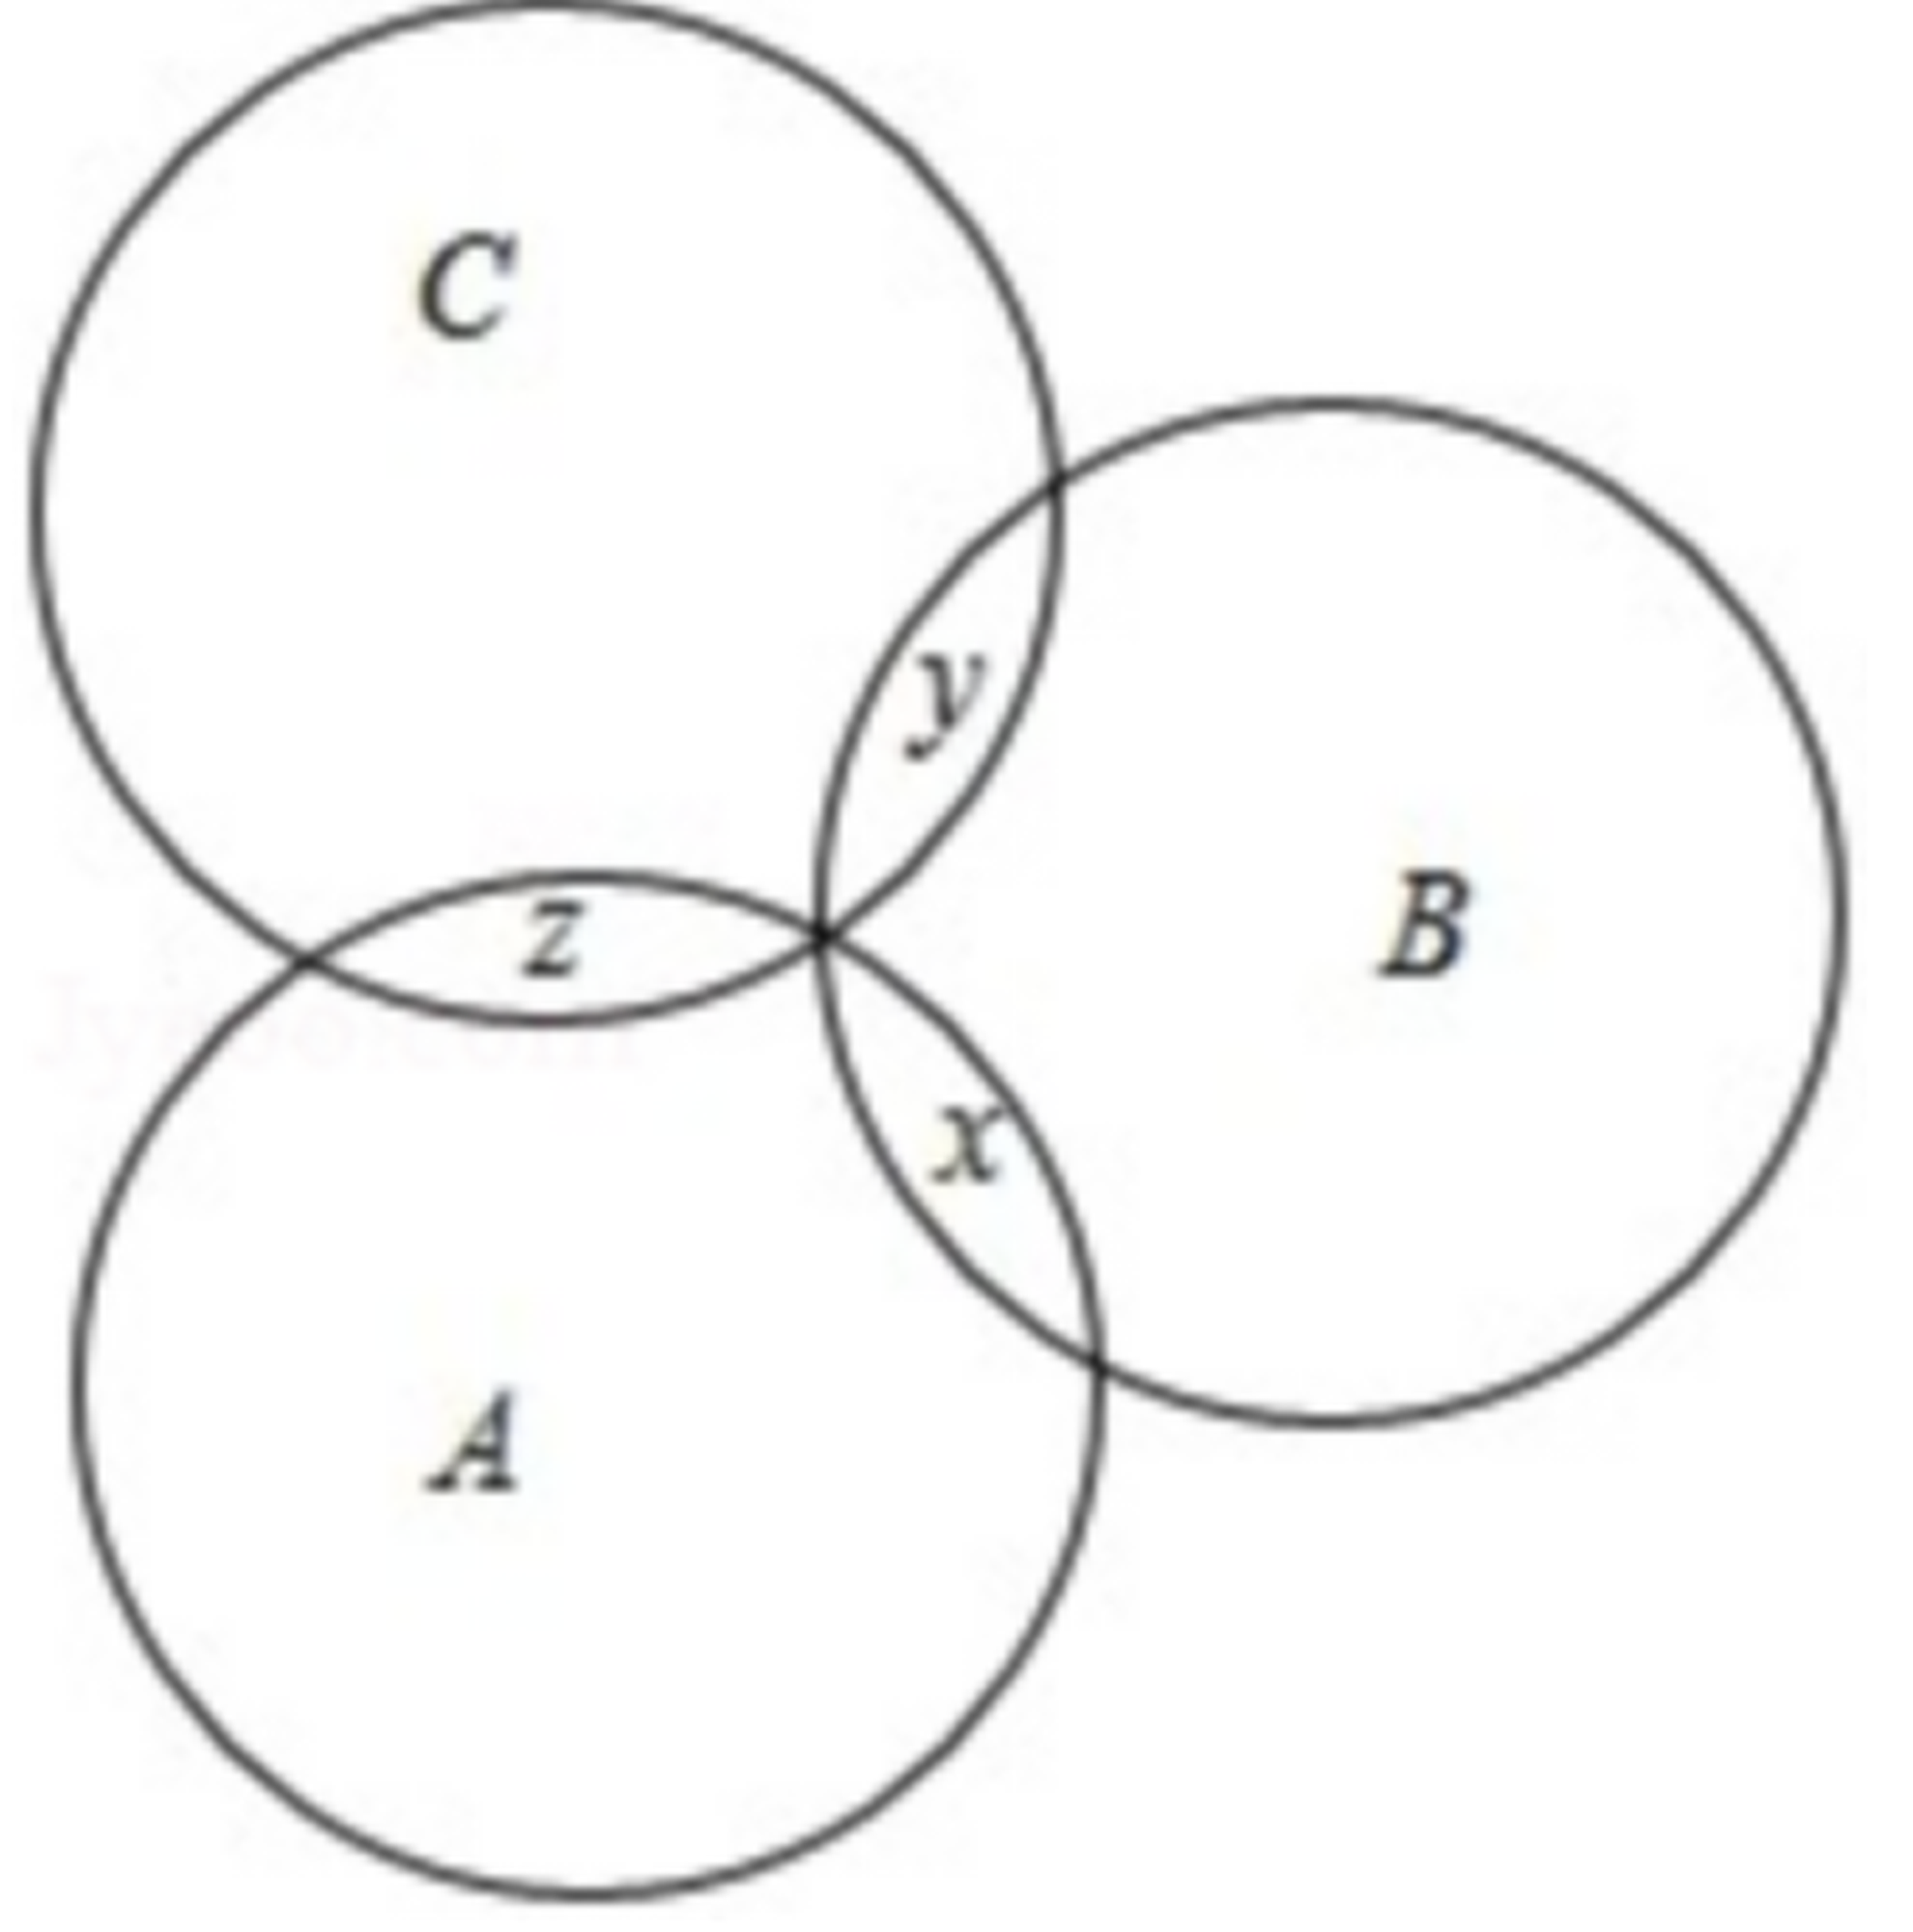
\includegraphics[width=0.30\textwidth]{figures/venn_ABC_x_y_z_h39.png}
\end{center}
\step{因为 $|A\cap B|=|B\cap C|=|C\cap A|=1$，且 $x$、$y$、$z\in\{1,2,3\}$，}
\step{所以集合 $A=\{x,z\}$，$B=\{x,y\}$，$C=\{z,y\}$，}
\step{若 $x=1$，$y=2$，$z=3$，则 $A=\{1,3\}$，$B=\{1,3\}$，$C=\{2,3\}$，}
\step{将 $1$，$2$，$3$ 进行全排列，有 $P_3^3=3\times2=6$ 个.}
\solend

\fi

\item 已知集合 $T=\{1,2,\cdots,2025\}$，对于 $T$ 的每一个非空子集的所有元素，计算它们乘积的倒数，
则所有这样倒数的和为 \blankline[4.4em].

\ans{$2025$}

\ifanswer
\solbegin
\step{集合 $T=\{1,2,\cdots,2025\}$ 的非空子集的个数为 $2^{2025}-1$，}
\step{这些子集中，每个元素的乘积分别为}
\step{$1,2,3,\cdots,2025,1\times2,1\times3,\cdots,1\times2025,\cdots,1\times2\times3\times\cdots\times2025$，}
\step{每项都可以看作是从 $1,2,3,\cdots,2025$ 中选择若干项的乘积，}
\step{$1+\dfrac12+\cdots+\dfrac{1}{2025}+\dfrac{1}{1\times2}+\dfrac{1}{1\times3}+\cdots+\dfrac{1}{2024\times2025}
+\cdots+\dfrac{1}{1\times2\times\cdots\times2025}$}
\step{$=(1+1)\left(1+\dfrac12\right)\cdots\left(1+\dfrac{1}{2025}\right)-1
=2\times\dfrac32\times\dfrac43\times\cdots\times\dfrac{2026}{2025}-1=2025$.}
\solend

\fi

% 第 24 题是压轴题，题干较长；试卷版在它之前量一次页高，尽量不与前文分家（照全稿成例）。
\ansneed{5cm}
% 注：原卷【解析】①③ 两步把 $f(x)$ 印作 $f[x[x]]$，显系笔误，照录未改，见文件头「笔误/存疑」⑦。
\item 若 $X$ 是一个集合，$T$ 是一个以 $X$ 的某些子集为元素的集合，且满足：①$X$ 属于 $T$，
$\varnothing$ 属于 $T$；②$T$ 中任意多个元素的并集属于 $T$；③$T$ 中任意多个元素的交集属于 $T$.
则称 $T$ 是集合 $X$ 上的一个拓扑. 已知函数 $f(x)=[x[x]]$，其中 $[x]$ 表示不大于 $x$ 的最大整数，
当 $x\in(0,n]$，$n\in\N^*$ 时，函数 $f(x)$ 值域为集合 $A_n$，则集合 $A_2$ 上的含有 $4$ 个元素的
拓扑 $T$ 的个数为 \blankline[4.4em].

\ans{$9$}

\ifanswer
\solbegin
\step{由题意，$n=2$，故 $0<x\leqslant2$，}
\step{①当 $0<x<1$ 时，则 $[x]=0$，所以 $f[x[x]]=0$，}
\step{②当 $x=1$ 时，$[x]=1$ 显然 $f(1)=1$，}
\step{③当 $1<x<2$ 时，$[x]=1$，所以 $f[x[x]]=[x]=1$，}
\step{④当 $x=2$ 时，$f(2)=4$，}
\step{所以 $A_2=\{0,1,4\}$，}
\step{因为 $T$ 中含有 $4$ 个元素，其中两个元素 $\varnothing$ 和 $A_2$，}
\step{$A_2=\{0,1,4\}$. 其它两个元素为 $A$、$B$，则
$\begin{cases}A\neq\varnothing\\ A\neq A_2\\ B\neq\varnothing\\ B\neq A_2\\ A\neq B\end{cases}$，}
\step{由对称性，不妨设 $1\leqslant|A|\leqslant|B|\leqslant2$，其中 $|A|$、$|B|$ 表示集合 $A$ 中元素的个数，}
\step{因为 $\begin{cases}A\cap B\in T\\ A\cup B\in T\end{cases}$，又 $|A|\leqslant|B|$，所以 $A\cap B=\varnothing$ 或 $A$，}
\step{若 $A\cap B=\varnothing$，则 $A\cup B$ 只能等于 $A_2$，}
\step{（若 $A\cup B=B$，则 $A\sub B$，则 $A\cap B=A=\varnothing$，矛盾）}
\step{则必有 $\begin{cases}|A|=1\\ |B|=2\end{cases}$，所以 $(A,B)$ 的个数 $\Leftrightarrow$ $A$ 的个数 $=3$ 种，}
\step{即 $\begin{cases}A=\{0\}\\ B=\{1,4\}\end{cases}$ 或 $\begin{cases}A=\{1\}\\ B=\{0,4\}\end{cases}$
或 $\begin{cases}A=\{4\}\\ B=\{0,1\}\end{cases}$；}
\step{若 $A\cap B=A\Leftrightarrow A\sub B$ 此时满足 $A\cup B=B$，}
\step{因为 $A\neq B$ 且 $1\leqslant|A|$ 且 $|B|\leqslant2$，所以 $\begin{cases}|A|=1\\ |B|=2\end{cases}$，}
\step{所以 $B$ 的选择共有 $C_3^2=3$ 种，则 $A$ 的个数有 $C_2^1$ 种，}
\step{所以 $(A,B)$ 的个数 $=2\times3=6$ 种.}
% 这六组「$A$／$B$」按原卷排作两行（前五个一行、第六个另起一行）；因五组并排时
% amsmath 的 cases 会为每组的第二列各留一枚 \quad，本行改排 \left\{\begin{matrix}…\end{matrix}\right.
% 以省下这枚 \quad（照 README「说明」记的高一07 成例），字形与 cases 相同。
\step{（这 $6$ 种是 $\left\{\begin{matrix}A=\{0\}\\ B=\{0,1\}\end{matrix}\right.$、
$\left\{\begin{matrix}A=\{1\}\\ B=\{0,1\}\end{matrix}\right.$、
$\left\{\begin{matrix}A=\{0\}\\ B=\{0,4\}\end{matrix}\right.$、
$\left\{\begin{matrix}A=\{4\}\\ B=\{0,4\}\end{matrix}\right.$、
$\left\{\begin{matrix}A=\{1\}\\ B=\{1,4\}\end{matrix}\right.$、}
\step{$\left\{\begin{matrix}A=\{4\}\\ B=\{1,4\}\end{matrix}\right.$）.}
\step{综上，$T$ 的个数为 $9$ 个.}
\solend

\fi

\end{enumerate}

\end{document}
"
%
% 原始材料是微信公众号图文（公众号「魔都数学加油站」连载「27学年高一 39」，署名「破晓」，
% 2026-09-26 21:29 发布，原文标题「27学年高一39——2026-2027年上海市大同中学高一上周末作业4.1」，
% 原文链接 https://mp.weixin.qq.com/s/HR2hIayXUXNi4zTs3PioiQ ），正文为 11 张 PNG 页。**同一篇里各页分辨率不一致**（2560×3620 与 4762×6735 两档混排：第 1、3、8、10 页为
% 2560×3620，第 2、4、5、6、7、9、11 页为 4762×6735）。原文本身就是一份**讲评版**——除第 15 题
% 外各题题下直接印【解析】（无单独的【答案】行），第 15 题的答案「D」直接印在题干末尾的括号内。
% 试题文字、答案与解析均照原卷录入，未改内容。卷面的粉色斜水印「魔都数学加油站」属水印，未录入。
%
% 卷首标题：原卷页首印作「2026-2027 年大同中学高一上周末作业 4.1」（**卷面标题行即带校名**，
% 年份区间按全稿惯例排 en dash，前缀照原卷保留「年」）。
%
% 篇幅与题号：卷面自「一、填空题」的**第 3 题**起编，终于「附加题」的**第 24 题**，共 22 题
% （填空 3—12、选择 13—16、解答 17—20、附加题 21—24）。第 1、2 题未在该文中发布——这是该
% 公众号连载讲评版的通例（高一02—高一09 等均自第 3 题起编，README「说明」已记），**不是截断**，
% 故本稿题号亦自 3 起。它与 高一40（大同中学 周末作业4.2）同属「周末作业 4」系列但**各自独立起编**
% （4.2 自第 3 题起、终于第 19 题），不是同一份试卷的两半。
%
% 与原卷的排版差异（均已在 README「说明」中交代）：
%   ① 原文自**第 3 题**起（第 1、2 题未在该文中发布），故本稿题号亦自 3 起，填空题以
%      \setcounter{enumi}{2} 起编；选择、解答、附加题三节各按上一节末号另设 \setcounter
%      （选择题 \setcounter{enumi}{12}、解答题 \setcounter{enumi}{16}、附加题 \setcounter{enumi}{20}）；
%   ② 原卷本就印有「一、填空题」「二、选择题」「三、解答题」三节标题，末节印作「附加题」
%      （**不带「四、」**，且题号 21—24 续前编、不另起），本稿照原卷分节，只把标题改排成全稿
%      统一的「大节标题」样式；
%   ③ 原卷是「讲评版」：除第 15 题外，各题题下均印【解析】（**全卷无一条独立的【答案】行**）；
%      第 15 题无解析，答案「D」直接印在题干末尾的括号内。本稿统一改为试卷版隐去、答案版以
%      \ans{}／\ifanswer 块给出，两版彻底分离；原卷写在【解析】末句的结果，本稿照 高一38
%      （同校同系列、同为讲评版）的成例另提为 \ans{}；
%   ④ 数集记号原卷两套并用：实数集作斜体的 $R$（第 7、11、14、17、18、19 题），整数集作斜体
%      $Z$（第 10 题），自然数集作斜体 $N$ 及 $N^*$（第 16、20、21、24 题），本稿按全稿惯例
%      统一写作 $\R$、$\Z$、$\N$、$\N^*$；
%   ⑤ 补集符号原卷两套并用：第 7 题作前缀式的 $C_U$（且题干称全集为 $I$，见「笔误/存疑」①），
%      第 14、15、18 题作上横线（$\overline{H}$、$\overline{A}$、$\overline{B}$），本稿照录、不归一
%      （前缀式写作 $\complement_U$，与 高一c／高一10 的成例一致）；
%   ⑥ 包含符号原卷两套并用：第 3 题作**无下划线**的 $\subset$，第 15、18、20、24 题作**带下划线**
%      的 $\sub$，本稿照录、不归一；
%   ⑦ 原卷填空的横线约两个字宽，本稿按全稿惯例统一排 \blankline[4.4em]；
%   ⑧ 第 7、11、22 题各有插图，取原卷截图、4× LANCZOS 放大（figures/venn_N_cap_CI_M_h39.png、
%      figures/plane_grid_4squares_h39.png、figures/venn_ABC_x_y_z_h39.png）；第 7 题的 Venn 属
%      **题干**（试卷版、答案版都出），第 11、22 题的图在【解析】内（仅答案版出）。第 7 题图
%      左下、第 11 题图的上／左／右边缘带进极淡的原卷粉色水印残影——照全稿「插图直接取自
%      原卷截图、不用 TikZ 重绘、不修图」的体例保留（再裁会切到坐标轴与 $x$、$y$、$O$ 标注）；
%   ⑨ 原卷并列的字母、数字（「$x_1,x_2$」「$a,b$」「$1,2,3,\cdots,11$」）多作半角逗号或不加标点，
%      本稿按全稿惯例改排顿号（$x_1$、$x_2$）或把数列并入行内公式；半角括号、逗号一律排全角，
%      数学式内部的标点照原样；
%   ⑩ 原卷未印副标题，本稿按**本卷实际内容**补出副标题「集合与常用逻辑用语」（依据见下条）。
%
% 副标题（\examtitlest 第二个参数）：本卷卷面未印副标题，由本稿补出，取值按 2026-09-26 起的
%   新口径「只用本卷实际内容的模块名」定为「集合与常用逻辑用语」。依据：全卷 22 题（第 3—24 题）中，
%   第 3、5、7、8、10、11、14、15、16、17、18、19、20、21、22、23、24 题共 17 题是集合的运算与
%   关系、子集／真子集、补集、集合新定义（「全食／偏食」、最小相交、拓扑、特征数）与集合计数，
%   以及命题与常用逻辑用语（第 3 题充要条件、第 5 题存在量词命题、第 17 题命题真假）；其余两题
%   第 4、6 考一元二次方程的根（韦达定理）与方程恒等，第 9、12、13 题是不等式（一元二次不等式组
%   的整数解、一元二次不等式解集、不等式的性质）——不等式合计 3/22，**不足全卷三分之一**，
%   故不并标「不等式」。
%
% 原卷笔误/存疑（均照抄原卷、未改，见源码中该处上方注释）：
%   ① 第 7 题题干称「全集 $I=R$」，而【解析】两处把补集写作 $C_U M$（下标作 $U$），前后记号不一；
%      本稿照录，未改；
%   ② 第 4 题【解析】两处把判别式印作 $\triangle=[2(m-1)^2-16m^2]$（方括号内首项漏了平方，
%      正确应作 $[2(m-1)]^2-16m^2$）；按其所判「$m=\frac12$ 时 $<0$、$m=-\frac12$ 时 $>0$」反推，
%      $[2(m-1)]^2-16m^2$ 在 $m=\frac12$ 时为 $-3<0$、在 $m=-\frac12$ 时为 $5>0$，与结论一致；
%      本稿照录；
%   ③ 第 9 题【解析】把方程组第二式印作 $1-2<-k\leqslant3$，按其结论 $-3\leqslant k<2$ 反推，
%      疑当作 $-2<-k\leqslant3$（原卷多一个「$1$」）；本稿照录；
%   ④ 第 17 题【解析】首句「由数 $y=-x^2+ax-1=-x+3$」中的「由数」显系「由」或「由函数」之误；
%      且末段「若 $p$ 真 $q$ 假…得 $a\in R$」「若 $p$ 假 $q$ 真…此时 $a$ 无解」与结论「$a$ 的取值范围
%      是 $R$」自相矛盾（按 $p:a\leqslant-5$、$q:a>-6$，$p$ 真 $q$ 假应为 $a\leqslant-6$，$p$ 假 $q$ 真
%      应为 $a>-5$，合起来是 $a\leqslant-6$ 或 $a>-5$，并非 $R$）；本稿一律照录，未按正确解法改写；
%   ⑤ 第 18 题【解析】(2) 把 $B=\{x\mid x^2+a\leqslant0\}$（$a<0$）印作右端开的
%      $\{x\mid-\sqrt{-a}\leqslant x<\sqrt{-a}\}$（应为闭的「$\leqslant$」）；按其所判
%      $\sqrt{-a}<\frac12$ 反推，不影响结论；本稿照录；
%   ⑥ 第 22 题【解析】在 $x=1$、$y=2$、$z=3$ 时把 $B=\{x,y\}$ 印作 $\{1,3\}$（应为 $\{1,2\}$），
%      与本行前面「$B=\{x,y\}$」不合；本稿照录；
%   ⑦ 第 24 题【解析】①③ 两步把 $f(x)$ 印作 $f[x[x]]$，显系笔误；本稿照录。
%   ⑧ 第 8 题【解析】「即方程 $x^2+ax+b=x$，$x^2+(a-1)x+b=0$ **由**两个相等的实数根为 $4$」——
%      「由」当为「有」（「设…是…有」的杂糅）；本稿照录；
%   ⑨ 第 10 题：题设 $a\oplus b=b(a^2+b^2+1)$，而集合定义里含 $\dfrac{a\oplus b}{2b}$；$-2<a<b<2$、
%      $a$、$b\in\Z$ 时 $(a,b)=(-1,0)$ 也合条件、却使分母 $2b=0$，原卷解析仍代入该组并约去
%      $b$ 得 $x=1$（答案集恰好不变）；本稿照录；
%   ⑩ 第 15 题选项列里 ② 与 ③ 之间**漏排分隔号**（原卷作「② $\overline{A}\cap B=\varnothing$③
%      $\overline{A}\sub\overline{B}$；」——①、③ 后都有「；」，② 后没有）；本稿照录；
%   ⑪ 第 20(2) 把 $\{1,2,\cdots,20\}$ 分成的 11 个集合里，$\{8,11\}$ 与 $\{9,12\}$ 之间误用
%      **句号**「.」（同行其余处皆逗号）；本稿照录；
%   ⑫ 第 20(3)① 推理不严：原卷写「选 5 则不选 1、9；选 6 则不选 2、10；选 7 则不选 3、11；
%      则只剩 4、8」——但 4 与 8 相差 $4$、不能同选，该情形实际最多只能取 $4$ 个；末句结论
%      「不超过 $5$ 个」仍成立；本稿照录；
%   ⑬ 第 16 题【解析】两种下标并存：「所以在 $A_i$ 的特征数构成中」原卷作斜体 $A_i$，而
%      「要使 $X_1+X_2+X_3$ 最大（小），则（应）在集合 $A_1$ 中首先放置…」两处原卷作
%      **数字 $1$**（与同句 $X_1$ 的角标同形）；本稿照录、未归一。
%
% 图取原卷截图（依次见各处的 \includegraphics 前的注释），4× LANCZOS 放大。
\documentclass[a4paper,11pt]{article}
\usepackage{common}

\begin{document}

\examtitlest[3]{2026--2027 年大同中学高一上周末作业 4.1}{集合与常用逻辑用语}

\bigsec{一、填空题}

\begin{enumerate}
\setcounter{enumi}{2}

\item “$x\geqslant a$”是“$0<x<2$”的必要非充分条件，则实数 $a$ 的取值范围是 \blankline[4.4em].

\ans{$(-\infty,0]$}

\ifanswer
\solbegin
\step{因为 $x\geqslant a$ 是 $0<x<2$ 的必要非充分条件，所以 $(0,2)\subset[a,+\infty)$，所以 $a\leqslant0$，}
\step{则实数 $a$ 的取值范围是 $(-\infty,0]$.}
\solend

\fi

% 注：原卷$[2(m-1)^2-16m^2]$ 首项漏了平方（应为 $[2(m-1)]^2-16m^2$），照录未改，见文件头「笔误/存疑」②。
\item 若关于 $x$ 的方程 $x^2+2(m-1)x+4m^2=0$ 有两个实数根，且这两根互为倒数，则 $m=$ \blankline[4.4em].

\ans{$-\dfrac12$}

\ifanswer
\solbegin
\step{设 $x_1$、$x_2$ 是方程 $x^2+2(m-1)x+4m^2=0$ 有两个实数根，}
\step{则 $x_1x_2=4m^2=1$，解得 $m=\dfrac12$ 或 $m=-\dfrac12$，}
\step{又当 $m=\dfrac12$ 时，$\triangle=[2(m-1)^2-16m^2]<0$，舍去，}
\step{当 $m=-\dfrac12$ 时，$\triangle=[2(m-1)^2-16m^2]>0$，故 $m=-\dfrac12$.}
\solend

\fi

\item 已知命题：“存在 $x\in[1,2]$，使 $x^2+2x+a\geqslant0$”为真命题，则 $a$ 的取值范围是 \blankline[4.4em].

\ans{$a\geqslant-8$}

\ifanswer
\solbegin
\step{若存在 $x\in[1,2]$，使 $x^2+2x+a\geqslant0$，}
\step{则等价为存在 $x\in[1,2]$，使 $x^2+2x\geqslant-a$，}
\step{当存在 $x\in[1,2]$ 时，设 $y=x^2+2x=(x+1)^2-1$，则 $3\leqslant y\leqslant8$，}
\step{所以要使 $x^2+2x\geqslant-a$，则 $8\geqslant-a$，即 $a\geqslant-8$.}
\solend

\fi

\item 已知方程 $a(3x+2)+b(2x-3)=8x+3$ 有无穷多个解，则 $a:b=$ \blankline[4.4em].

\ans{$30:7$}

\ifanswer
\solbegin
\step{$a(3x+2)+b(2x-3)=(3a+2b)x+2a-3b=8x+3$ 有无穷多个解，}
\step{所以 $\begin{cases}3a+2b=8\\ 2a-3b=3\end{cases}$，解得 $a=\dfrac{30}{13}$，$b=\dfrac{7}{13}$，所以 $a:b=30:7$.}
\solend

\fi

% 注：原卷题干称「全集 $I=R$」，而【解析】两处把补集写作 $C_U M$（下标作 $U$），前后记号不一；
%     照录未改，见文件头「笔误/存疑」①。
\item 已知集合 $M=\{x\mid y=\sqrt{3-x^2}\}$，$N=\{x\mid-3\leqslant x\leqslant1\}$，全集 $I=\R$，
则图中阴影部分表示的集合为 \blankline[4.4em].

% 图取原卷截图（01.png，2560×3620）右栏，4× LANCZOS 放大。
\begin{center}
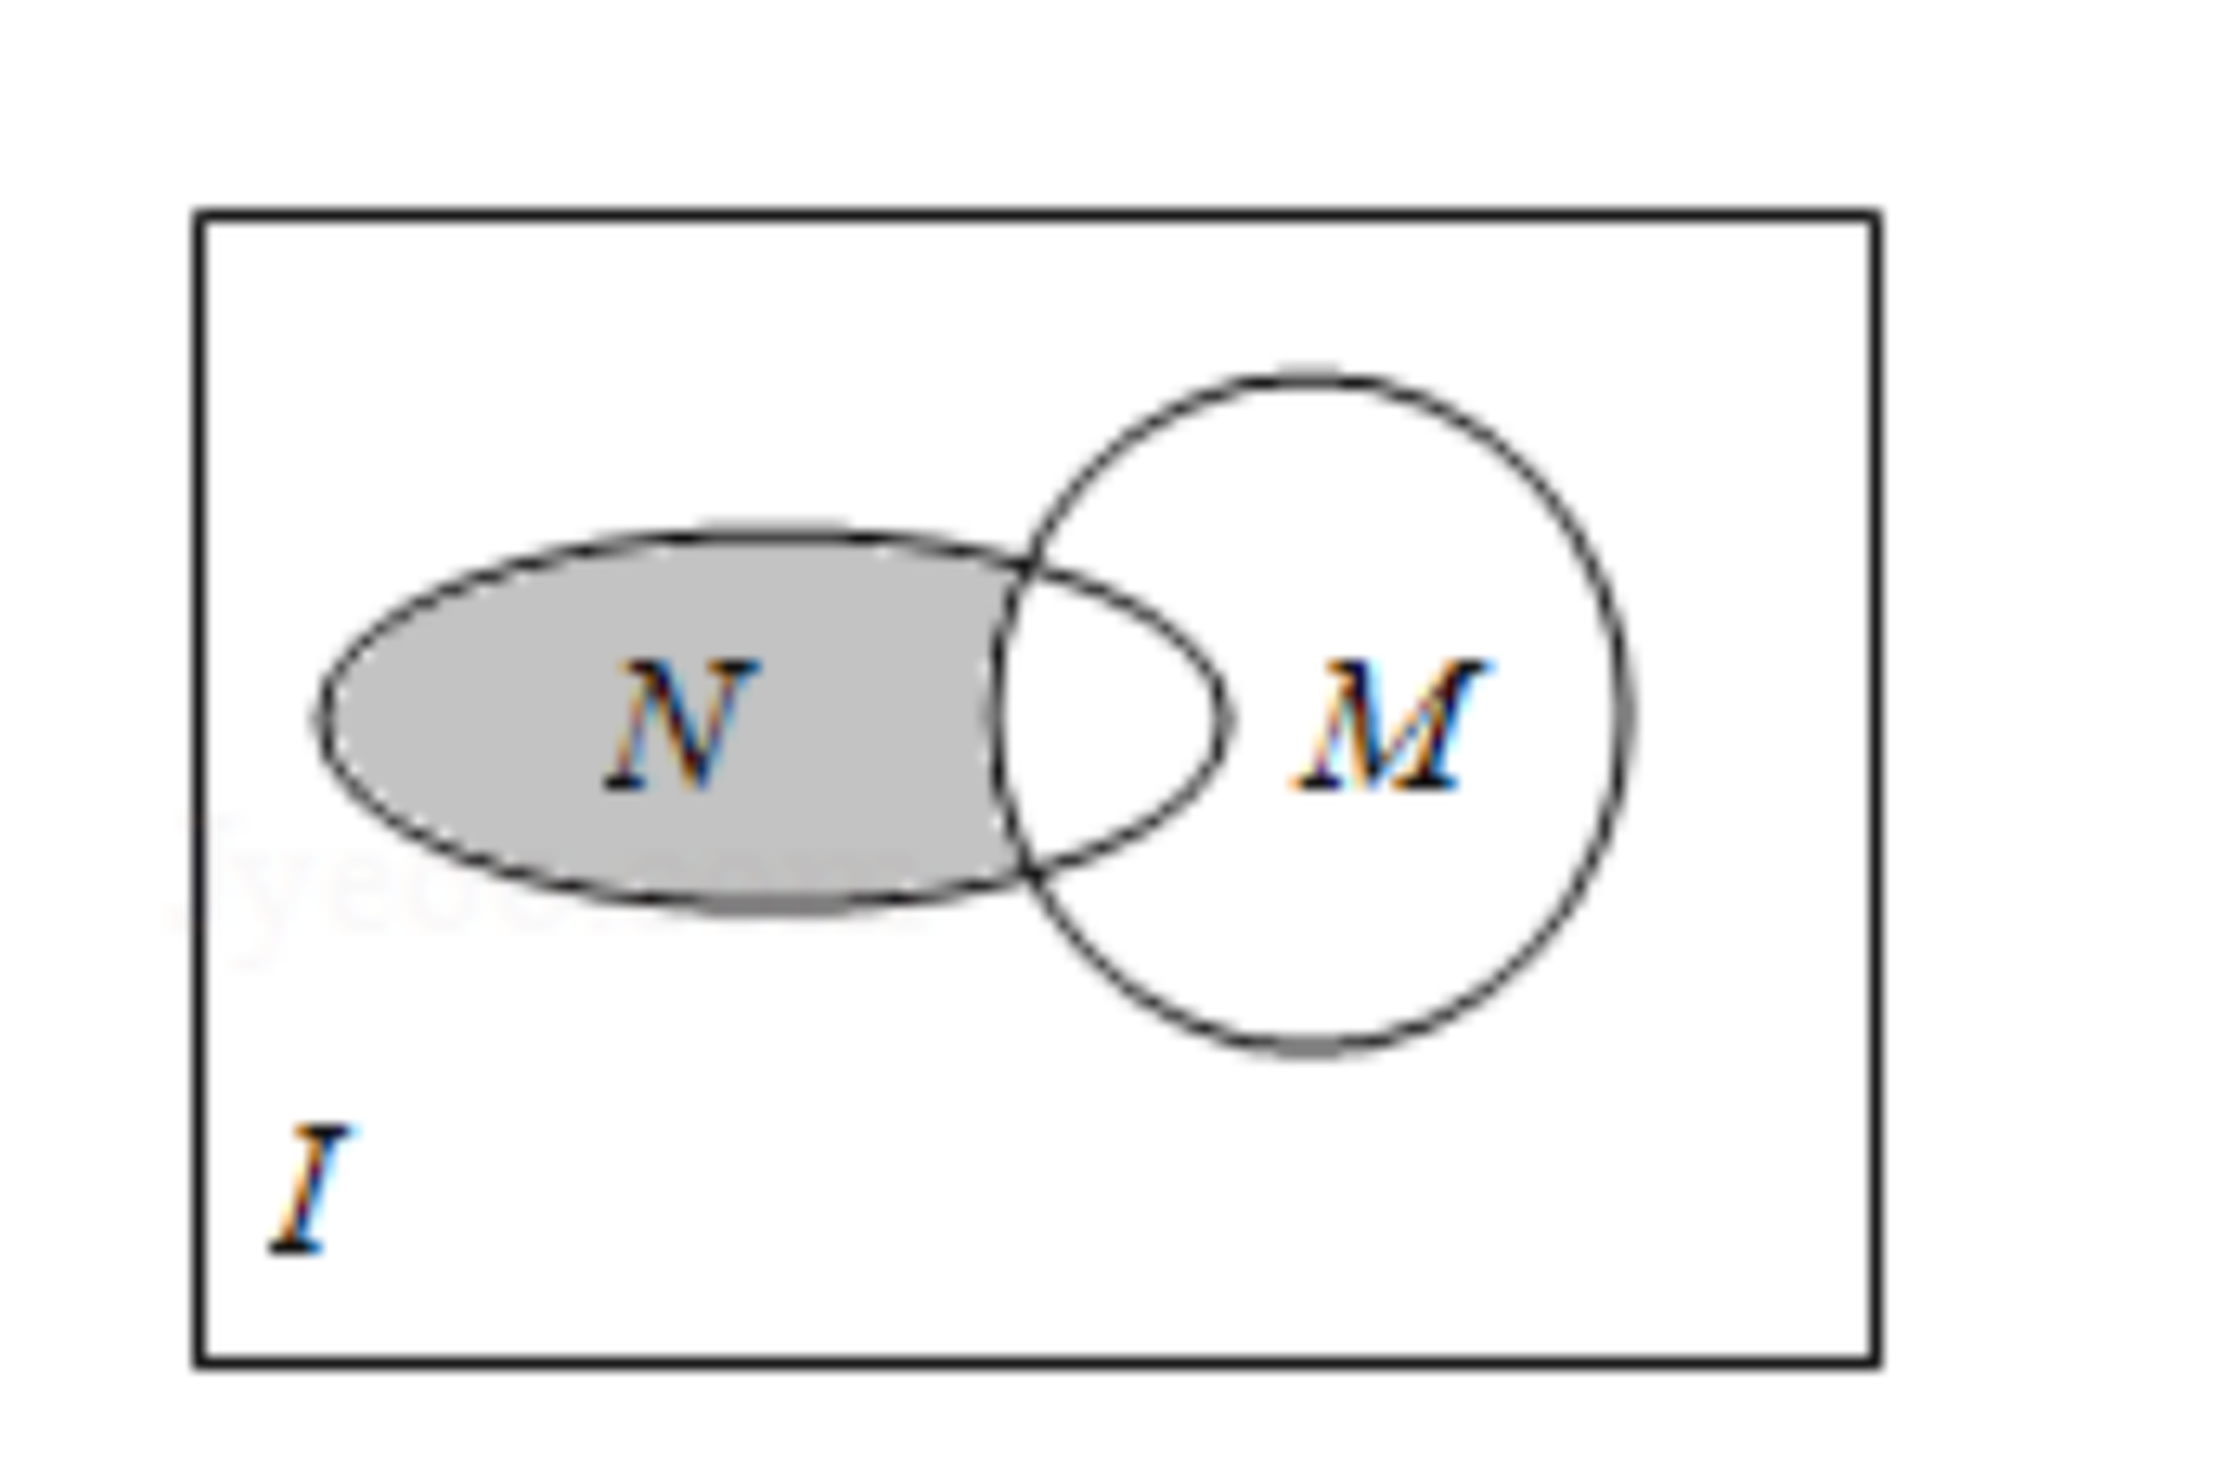
\includegraphics[width=0.30\textwidth]{figures/venn_N_cap_CI_M_h39.png}
\end{center}

\ans{$[-3,-\sqrt3)$}

\ifanswer
\solbegin
\step{阴影部分用集合表示为 $N\cap(\complement_UM)$.}
\step{则 $M=\{x\mid y=\sqrt{3-x^2}\}=\{x\mid3-x^2\geqslant0\}=\{x\mid-\sqrt3\leqslant x\leqslant\sqrt3\}$，}
\step{则 $\complement_UM=\{x\mid x>\sqrt3\text{ 或 }x<-\sqrt3\}$，$N=\{x\mid|x+1|\leqslant2\}=\{x\mid-3\leqslant x\leqslant1\}$，}
\step{则 $N\cap(\complement_UM)=\{x\mid-3\leqslant x<-\sqrt3\}$.}
\solend

\fi

\item 已知 $f(x)=x^2+ax+b$，集合 $\{x\mid f(x)=x\}=\{4\}$，将集合 $M=\{x\mid f(x)=4\}$ 用列举法表示 \blankline[4.4em].

\ans{$\{3,4\}$}

\ifanswer
\solbegin
\step{已知 $f(x)=x^2+ax+b$，集合 $\{x\mid f(x)=x\}=\{4\}$，}
% 注：原卷本行作「…$x^2+(a-1)x+b=0$ **由**两个相等的实数根为 $4$」——「由」当为「有」
%     （「设…是…有」的杂糅）；本稿照录未改，见文件头「原卷笔误/存疑」⑧。
\step{即方程 $x^2+ax+b=x$，$x^2+(a-1)x+b=0$ 由两个相等的实数根为 $4$，}
\step{所以 $\triangle=(a-1)^2-4b=0$，即 $x^2+(a-1)x+b=(x-4)^2$，所以 $b=16$，$a=-7$，}
\step{所以 $f(x)=x^2+ax+b=x^2-7x+16$，所以集合 $M=\{x\mid f(x)=4\}$，}
\step{即 $x^2-7x+16=4$，$x^2-7x+12=0$，故 $M=\{x\mid f(x)=4\}=\{3,4\}$.}
\solend

\fi

% 注：原卷方程组第二式印作 $1-2<-k\leqslant3$，按其结论 $-3\leqslant k<2$ 反推疑当作 $-2<-k\leqslant3$，
%     照录未改，见文件头「笔误/存疑」③。
\item 关于 $x$ 的不等式组 $\begin{cases}x^2-x-2>0\\ 2x^2+(2k+5)x+5k<0\end{cases}$ 的整数解的集合为 $\{-2\}$，
则实数 $k$ 的取值范围 \blankline[4.4em].

\ans{$-3\leqslant k<2$}

\ifanswer
\solbegin
\step{原不等式组即 $\begin{cases}(x-2)(x+1)>0\\ (x+k)(2x+5)<0\end{cases}$，整数解的集合为 $A$，若 $A=\{-2\}$，}
\step{则 $(-2+k)(2\times(-2)+5)<0$，所以 $k<2$，且有 $\begin{cases}-k>-\dfrac52\\ 1-2<-k\leqslant3\end{cases}$，}
\step{解得 $-3\leqslant k<2$.}
\solend

\fi

\item 规定 $\oplus$ 与 $\otimes$ 是两个运算符号，其运算法则如下，对任意实数 $a$、$b$ 有：$a\otimes b=ab$，
$a\oplus b=b(a^2+b^2+1)$. 若 $-2<a<b<2$ 且 $a$、$b\in\Z$，
$A=\left\{x\mid x=2(a\otimes b)+\dfrac{a\oplus b}{2b}\right\}$，则用列举法表示集合 $A=$ \blankline[4.4em].

\ans{$\left\{1,-\dfrac12\right\}$}

\ifanswer
\solbegin
\step{$A=\left\{x\mid x=2(a\otimes b)+\dfrac{a\oplus b}{2b}\right\}
=\left\{x\mid x=2ab+\dfrac{b(a^2+b^2+1)}{2b}\right\}$}
\step{$=\left\{x\mid x=2ab+\dfrac12a^2+\dfrac12b^2+\dfrac12\right\}
=\left\{x\mid x=\dfrac12(a+b)^2+ab+\dfrac12\right\}$，}
% 注：题设含 $\dfrac{a\oplus b}{2b}$，而 $-2<a<b<2$、$a$、$b\in\Z$ 时 $(a,b)=(-1,0)$ 也合条件、
%     却使分母 $2b=0$；原卷解析仍代入该组并约去 $b$ 得 $x=1$（答案集恰好不变）。本稿照录，
%     见文件头「原卷笔误/存疑」⑨。
\step{当 $a=-1$，$b=0$ 时，$x=1$；当 $a=-1$，$b=1$ 时，$x=-\dfrac12$；}
\step{当 $a=0$，$b=1$ 时，$x=1$；所以 $A=\left\{1,-\dfrac12\right\}$.}
\solend

\fi

\item 高斯是德国著名的数学家，近代数学奠基者之一，享有“数学王子”的称号，为了纪念数学家高斯，
我们把取整函数 $y=[x]$，$x\in\R$ 称为高斯函数，其中 $[x]$ 表示不超过 $x$ 的最大整数，
如 $[1.1]=1$，$[-1.1]=-2$. 则点集 $P=\{(x,y)\mid[x]^2+[y]^2=1\}$
所表示的平面区域的面积是 \blankline[4.4em].

\ans{$4$}

\ifanswer
\solbegin
\step{$[x]^2+[y]^2=1$ 由 $\begin{cases}[x]=0\\ [y]=-1\end{cases}$ 或 $\begin{cases}[x]=0\\ [y]=1\end{cases}$
或 $\begin{cases}[x]=-1\\ [y]=0\end{cases}$ 或 $\begin{cases}[x]=1\\ [y]=0\end{cases}$ 四个平面区域组成，}
\step{即 $\begin{cases}0\leqslant x<1\\ -1\leqslant y<0\end{cases}$ 或 $\begin{cases}0\leqslant x<1\\ 1\leqslant y<2\end{cases}$
或 $\begin{cases}-1\leqslant x<0\\ 0\leqslant y<1\end{cases}$ 或 $\begin{cases}1\leqslant x<2\\ 0\leqslant y<1\end{cases}$，}
\step{作出平面区域如图所示，平面区域由四个边长为 $1$ 的正方形组成，}
% 图在【解析】内（仅答案版出），取原卷截图（03.png，2560×3620）中部，4× LANCZOS 放大。
\begin{center}
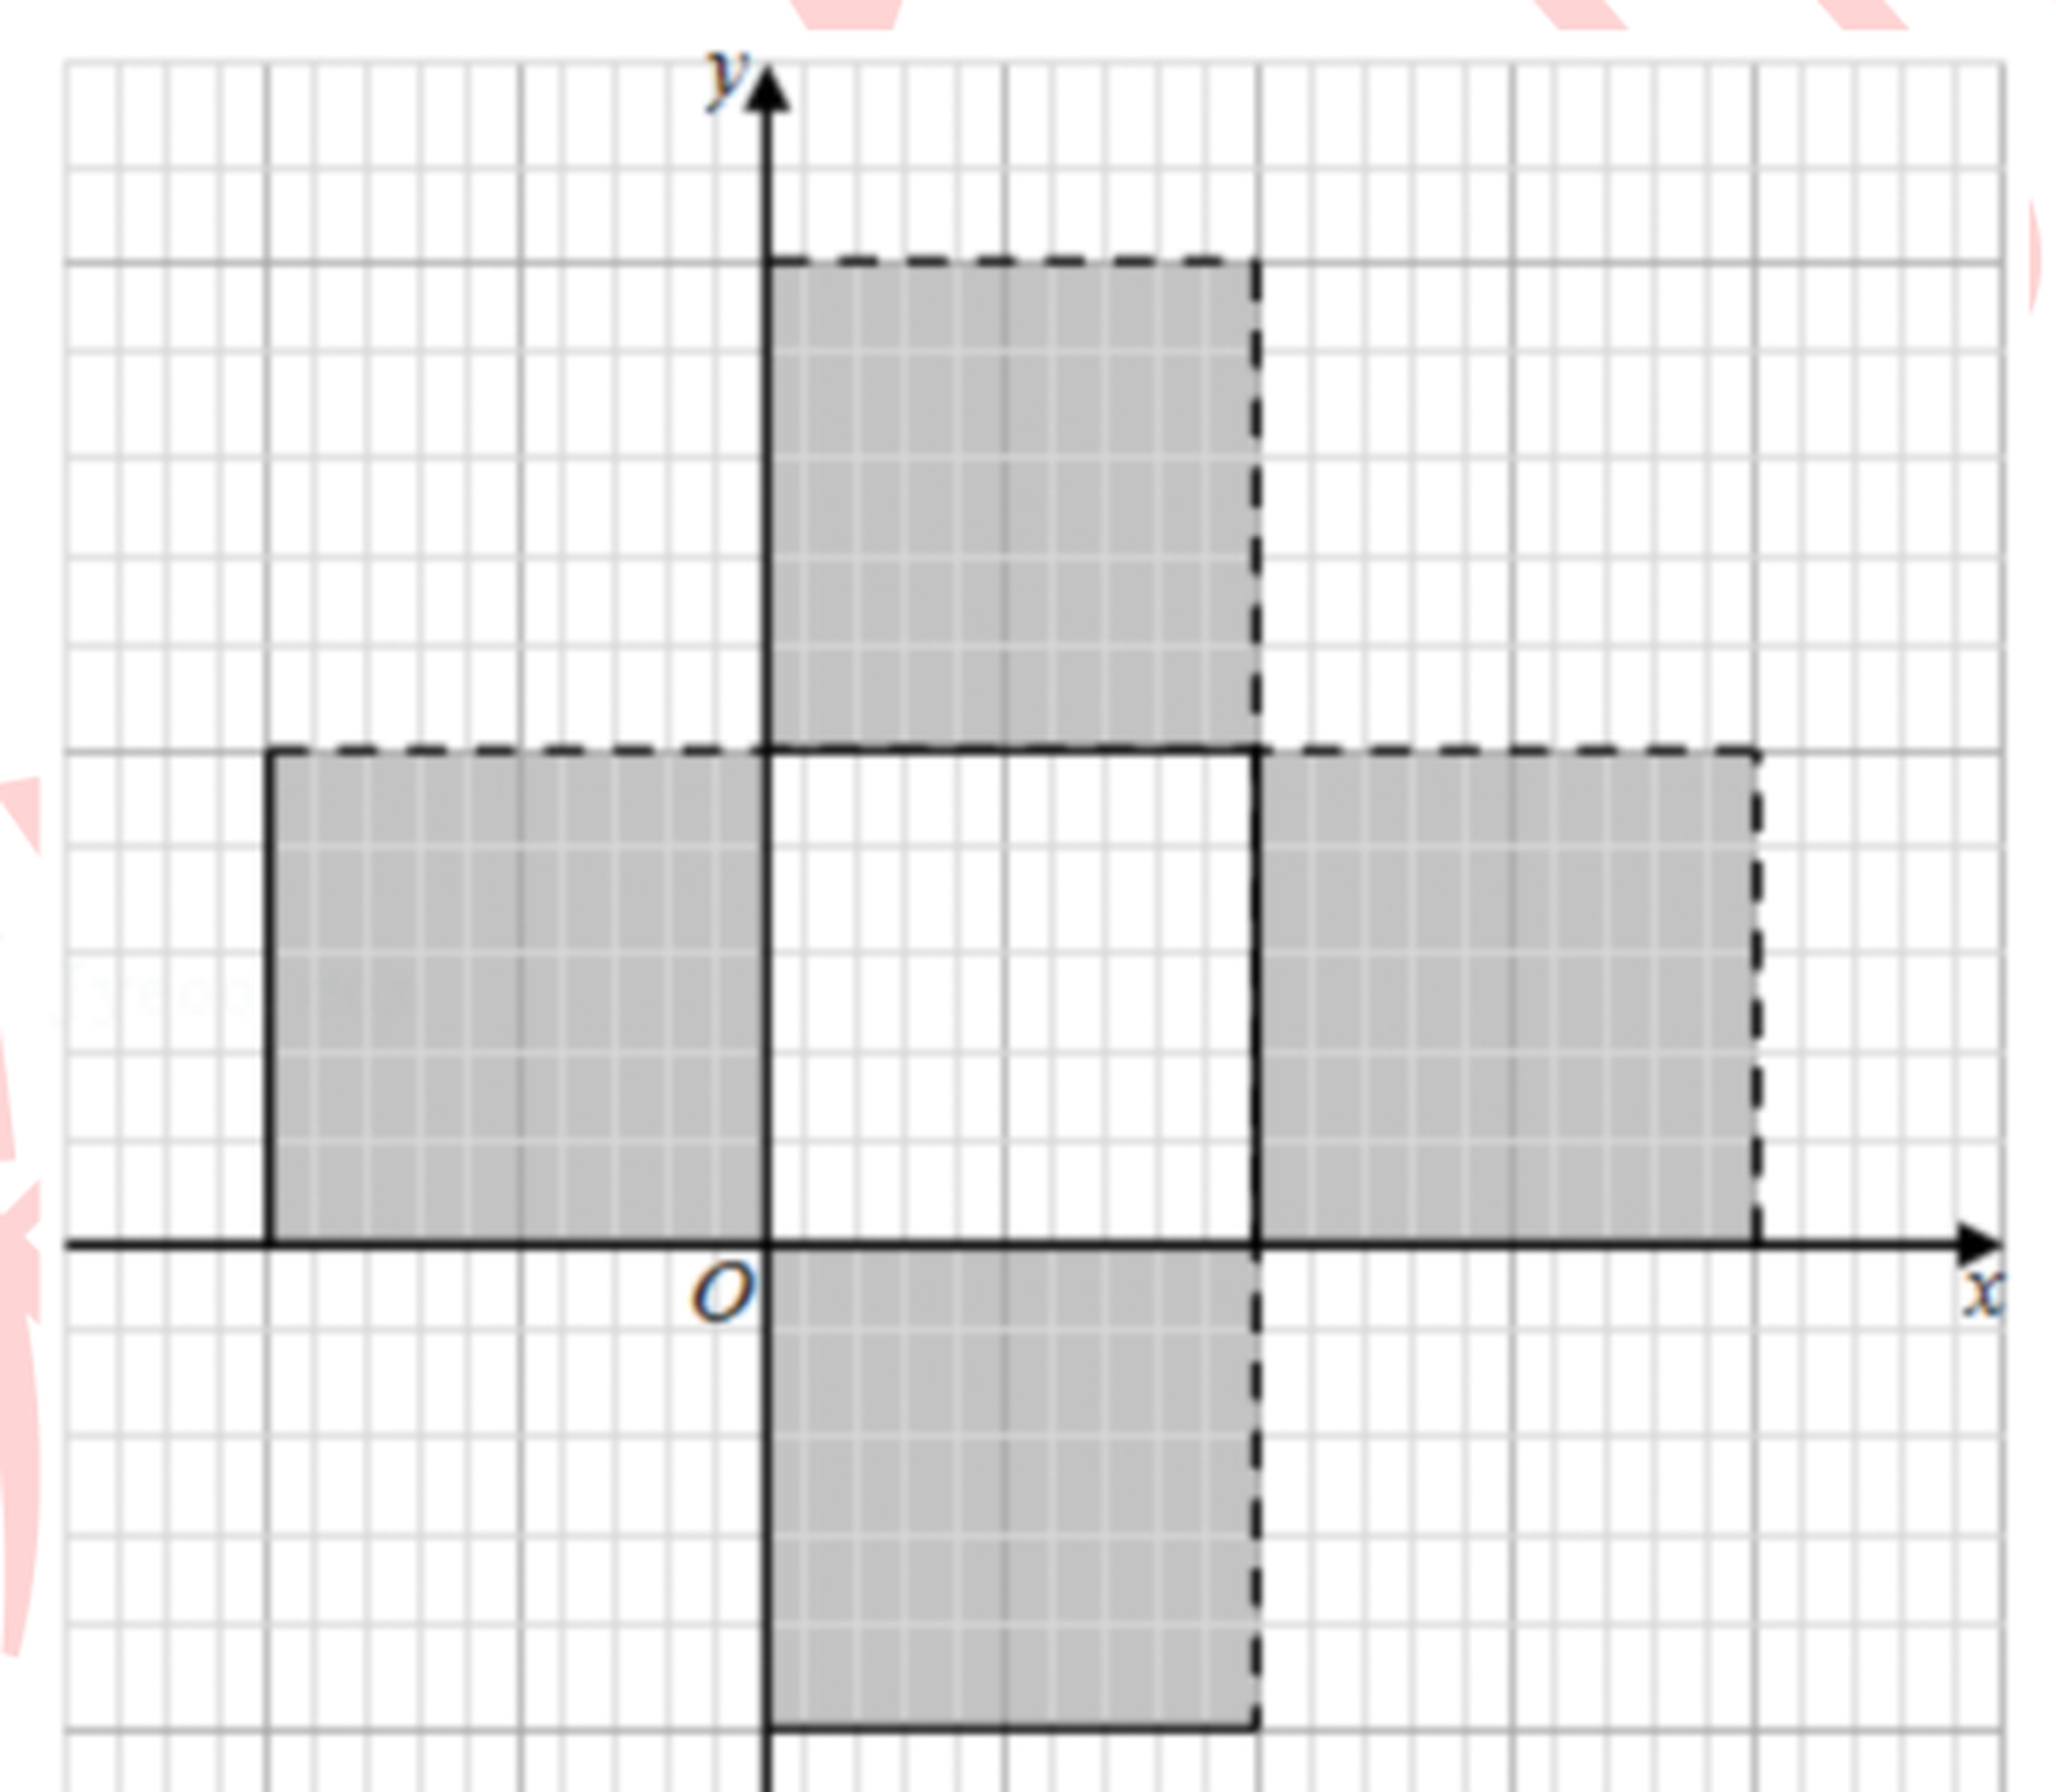
\includegraphics[width=0.38\textwidth]{figures/plane_grid_4squares_h39.png}
\end{center}
\step{总面积为 $1\times4=4$.}
\solend

\fi

\item 关于 $x$ 的不等式 $ax^2+bx+c>0$ 的解集为 $\{x\mid x<\beta\text{ 或 }x>\gamma\}(0<\beta<\gamma)$，
则不等式 $a(x^2+1)+b(x-1)+c>2ax$ 的解集为 \blankline[4.4em].

\ans{$(-\infty,\beta+1)\cup(\gamma+1,+\infty)$}

\ifanswer
\solbegin
\step{由题意得 $\beta$、$\gamma$ 为方程 $ax^2+bx+c=0$ 的两根且 $a>0$，}
\step{则 $\beta+\gamma=-\dfrac ba$，$\beta\gamma=\dfrac ca$，故 $b=-a(\beta+\gamma)$，$c=\beta\gamma a$，}
\step{则不等式可化为 $a(x^2+1)-a(\beta+\gamma)(x-1)+\beta\gamma a>2ax$，}
\step{因为 $a>0$，所以 $x^2+1-(\beta+\gamma)(x-1)+\beta\gamma>2x$，}
\step{即 $x^2-(\beta+\gamma+2)x+(\beta+\gamma+\beta\gamma+1)>0$，所以 $(x-\beta-1)(x-\gamma-1)>0$，}
\step{解得 $x<\beta+1$ 或 $x>\gamma+1$，所以不等式解集为 $(-\infty,\beta+1)\cup(\gamma+1,+\infty)$.}
\solend

\fi

\end{enumerate}

\bigsec{二、选择题}

\begin{enumerate}
\setcounter{enumi}{12}

\item 设 $a<b<0$，则下列不等式中不成立的是\mbox{（\quad）}

\keepwithprev
A. $\dfrac1a>\dfrac1b$\qquad B. $\dfrac{1}{a-b}>\dfrac1a$\qquad C. $|a|>-b$\qquad D. $\sqrt{-a}>\sqrt{-b}$

\ans{$B$}

\ifanswer
\solbegin
\step{令 $a=-2$，$b=-1$，}
\step{A、$-\dfrac12>-1$，正确；B、$-1<-\dfrac12$，故 B 错误；C、$2>1$，正确；}
\step{D、$\sqrt2>1$，正确；故选 B.}
\solend

\fi

\item 设实数集 $\R$ 为全集，集合 $P=\{x\mid f(x)=0\}$，$Q=\{x\mid g(x)=0\}$，$H=\{x\mid h(x)=0\}$，
则方程 $\dfrac{f^2(x)+g^2(x)}{h(x)}=0$ 的解集是\mbox{（\quad）}

\keepwithprev
A. $P\cap Q\cap\overline{H}$\qquad B. $P\cap Q$\qquad C. $P\cap Q\cap H$\qquad D. $P\cap Q\cup H$

\ans{$A$}

\ifanswer
\solbegin
\step{方程 $\dfrac{f^2(x)+g^2(x)}{h(x)}=0$ 等价于 $\begin{cases}f(x)=0\\ g(x)=0\\ h(x)\neq0\end{cases}$，}
\step{又因为 $P=\{x\mid f(x)=0\}$，$Q=\{x\mid g(x)=0\}$，$H=\{x\mid h(x)=0\}$，}
\step{所以方程 $\dfrac{f^2(x)+g^2(x)}{h(x)}=0$ 的解集是 $P\cap Q\cap\overline{H}$，故选 A.}
\solend

\fi

\item 设全集 $U$，在下列条件中，是 $B\sub A$ 的充要条件的有\mbox{（\quad）}

\keepwithprev
% 注：原卷此行 ② 与 ③ 之间**漏排分隔号**（①、③ 后都有「；」，② 后没有）；
%     本稿照录未补，见文件头「原卷笔误/存疑」⑩。
①$A\cup B=A$；\qquad ②$\overline{A}\cap B=\varnothing$\qquad ③$\overline{A}\sub\overline{B}$；\qquad ④$A\cup\overline{B}=U$

\keepwithprev
A. $1$ 个\qquad B. $2$ 个\qquad C. $3$ 个\qquad D. $4$ 个

\ans{$D$}

\item 已知集合 $M=\{x\mid x\in\N,0<x\leqslant15\}$，$A_1$、$A_2$、$A_3$ 满足：①$A_1\cup A_2\cup A_3=M$；
②每个集合都恰有 $5$ 个元素. 集合 $A_i(i=1,2,3)$ 中最大元素与最小元素之和称为 $A_i$ 的特征数，
记为 $X_i(i=1,2,3)$，则 $X_1+X_2+X_3$ 的值不可能为\mbox{（\quad）}

\keepwithprev
A. $37$\qquad B. $39$\qquad C. $48$\qquad D. $57$

\ans{$A$}

\ifanswer
\solbegin
\step{因为集合 $M=\{x\mid x\in\N,0<x\leqslant15\}=\{1,2,3,\cdots,15\}$，}
\step{又因为集合 $A_1$、$A_2$、$A_3$ 中，每个集合恰有 $5$ 个元素，}
\step{且 $A_1\cup A_2\cup A_3=M$ 有 $15$ 个元素，所以集合 $A_1$、$A_2$、$A_3$ 中没有重复元素，}
\step{因为 $1$ 是集合 $M$ 中数值最小的元素，$15$ 是集合 $M$ 中数值最大的元素，}
\step{所以在 $A_i$ 的特征数构成中，必有 $1$ 和 $15$，不妨设 $1\in A_1$，$15\in A_1$，}
% 注：原卷本行（与下面「最小」那句）在「集合」后的角标是**数字 $1$**（同句 $X_1$ 的角标同形），
%     而非上一行「$A_i$ 的特征数构成」里的斜体 $A_i$——原卷两种下标并存，本稿照录、不归一，
%     见文件头「原卷笔误/存疑」⑬。
\step{要使 $X_1+X_2+X_3$ 最大，则应该在集合 $A_1$ 中首先放置数值较小的元素，}
\step{即 $A_1=\{1,2,3,4,15\}$，所以 $5$ 与 $14$ 是剩下元素中数值最小或最大的元素，}
\step{同理，不妨设 $5\in A_2$，$14\in A_2$，接着在 $A_2$ 中再次放置数值较小的元素，}
\step{即 $A_2=\{5,6,7,8,14\}$，则 $A_3=\{9,10,11,12,13\}$，}
\step{此时 $X_1+X_2+X_3$ 有最大值为 $1+15+5+14+9+13=57$，}
\step{即 $X_1+X_2+X_3\leqslant57$；}
% 注：同上一处——原卷此行角标是**数字 $1$**（$A_1$），本稿照录，未与「$A_i$」归一。
\step{要使 $X_1+X_2+X_3$ 最小，则在集合 $A_1$ 中首先放置数值较大的元素，}
\step{即 $A_1=\{1,12,13,14,15\}$，所以 $2$ 与 $11$ 是剩下元素中数值最小或最大的元素，}
\step{同理，不妨设 $2\in A_2$，$11\in A_2$，接着在 $A_2$ 中再次放置数值较大的元素，}
\step{即 $A_2=\{2,8,9,10,11\}$，则 $A_3=\{3,4,5,6,7\}$，}
\step{此时 $X_1+X_2+X_3$ 有最小值为 $1+15+2+11+3+7=39$，}
\step{即 $X_1+X_2+X_3\geqslant39$，}
\step{综上，$39\leqslant X_1+X_2+X_3\leqslant57$，故选 A.}
\solend

\fi

\end{enumerate}

\bigsec{三、解答题}

\begin{enumerate}
\setcounter{enumi}{16}

% 注：原卷首句「由数 $y=-x^2+ax-1=-x+3$」中的「由数」显系「由」或「由函数」之误；末段
%     的两处分类讨论与结论自相矛盾（详见文件头「笔误/存疑」④）。本稿一律照录，未改。
\item 命题 $p$：函数 $y=-x^2+ax-1$ 与 $y=-x+3$ 图象交点的横坐标均为负值，
命题 $q$：关于 $x$ 的方程 $2(1-x)a+(x^2-10x-3)=0$ 的两个根，一个大于 $3$，另一个小于 $3$；
若命题 $p$ 和命题 $q$ 中有且仅有一个是真命题，求 $a$ 的取值范围.

\ans{$\R$}

\ifanswer
\solbegin
\step{由数 $y=-x^2+ax-1=-x+3$ 得 $x^2-(a+1)x+4=0$，}
\step{若横坐标均为负值，则满足 $\begin{cases}\Delta=(a+1)^2-16\geqslant0\\ x_1x_2=4>0\\ x_1+x_2=a+1<0\end{cases}$
得 $\begin{cases}a\geqslant3\text{ 或 }a\leqslant-5\\ a<-1\end{cases}$，得 $a\leqslant-5$，}
\step{即 $p:a\leqslant-5$，}
\step{若方程 $2(1-x)a+(x^2-10x-3)=0$ 的两个根，一个大于 $3$，另一个小于 $3$；}
\step{设 $f(x)=2(1-x)a+(x^2-10x-3)$，则 $f(3)<0$，即 $-4a-24<0$，}
\step{得 $a>-6$，即 $q:a>-6$，}
\step{因为命题 $p$ 和命题 $q$ 中有且仅有一个是真命题，}
\step{若 $p$ 真 $q$ 假，则 $\begin{cases}a\leqslant-5\\ a>-6\end{cases}$，得 $a\in\R$，}
\step{若 $p$ 假 $q$ 真，则 $\begin{cases}a>-5\\ a\leqslant-6\end{cases}$，此时 $a$ 无解，}
\step{综上，实数 $a$ 的取值范围是 $\R$.}
\solend

\fi

\ansspace[8]

\item 设全集是实数集 $\R$，$A=\left\{x\mid\dfrac{1-2x}{x-3}\geqslant0\right\}$，$B=\{x\mid x^2+a\leqslant0\}$.

\begin{enumerate}[label=(\arabic*)]

\item 当 $a=-4$ 时，求 $A\cup B$；

\item 若 $\overline{A}\cap B=B$，求实数 $a$ 的取值范围.

\end{enumerate}

\ans{（1）$\{x\mid-2\leqslant x<3\}$；（2）$\left(-\dfrac14,+\infty\right)$}

\ifanswer
\solbegin
\stepm{(1)}{$A=\left\{x\mid\dfrac{1-2x}{x-3}\geqslant0\right\}=\left\{x\mid\dfrac12\leqslant x<3\right\}$，$B=\{x\mid x^2+a\leqslant0\}$.}
\step{当 $a=-4$ 时，$B=\{x\mid-2\leqslant x\leqslant2\}$，所以 $A\cup B=\{x\mid-2\leqslant x<3\}$.}
\stepm{(2)}{$\overline{A}=\left\{x\mid x\geqslant3\text{ 或 }x<\dfrac12\right\}$，$B=\{x\mid x^2+a\leqslant0\}$.}
\step{由 $\overline{A}\cap B=B$，得 $B\sub\overline{A}$，}
\step{则当 $a>0$ 时，$B=\varnothing$，满足 $B\sub\overline{A}$，则 $a>0$ 成立，}
\step{则当 $a=0$ 时，$B=\{0\}$，满足 $B\sub\overline{A}$，则 $a=0$ 成立，}
\step{当 $a<0$ 时，$B=\{x\mid-\sqrt{-a}\leqslant x<\sqrt{-a}\}$，}
\step{得 $\sqrt{-a}<\dfrac12$，即 $-\dfrac14<a<0$，}
\step{综上，实数 $a$ 的取值范围是 $\left(-\dfrac14,+\infty\right)$.}
\solend

\fi

\ansspace[6]

\item 设集合 $A=\{x\mid ax^2+2x+1=0,a\in\R\}$.

\begin{enumerate}[label=(\arabic*)]

\item 当 $A$ 中元素个数为 $1$ 时，求：$a$ 和 $A$；

\item 当 $A$ 中元素个数至少为 $1$ 时，求：$a$ 的取值范围；

\item 求：$A$ 中各元素之和.

\end{enumerate}

\ans{（1）$a=0$ 时 $A=\left\{-\dfrac12\right\}$，$a=1$ 时 $A=\{-1\}$；（2）$(-\infty,1]$；
（3）$a=0$ 时和为 $-\dfrac12$，$a<1$ 且 $a\neq0$ 时和为 $-\dfrac2a$，$a=1$ 时和为 $-1$，$a>1$ 时 $A$ 中无元素}

\ifanswer
\solbegin
\stepm{(1)}{集合 $A=\{x\mid ax^2+2x+1=0,a\in\R\}$，$A$ 中元素个数为 $1$，}
\step{所以 $a=0$ 或 $\begin{cases}a\neq0\\ \Delta=4-4a=0\end{cases}$，解得 $a=0$，$A=\left\{-\dfrac12\right\}$ 或 $a=1$，$A=\{-1\}$.}
\stepm{(2)}{当 $A$ 中元素个数至少为 $1$ 时，$a=0$ 或 $\begin{cases}a\neq0\\ \Delta=4-4a\geqslant0\end{cases}$，解得 $a\leqslant1$，}
\step{所以 $a$ 的取值范围是 $(-\infty,1]$.}
\stepm{(3)}{当 $a=0$ 时，$A$ 中元素之和为 $-\dfrac12$；}
\step{当 $a<1$ 且 $a\neq0$ 时，$A$ 中元素之和为 $-\dfrac2a$；}
\step{当 $a=1$ 时，$A$ 中元素之和为 $-1$；}
\step{当 $a>1$ 时，$A$ 中无元素.}
\solend

\fi

\ansspace[8]

\item 设 $k$ 是正整数，集合 $A$ 至少有两个元素，且 $A\sub\N^*$. 如果对于 $A$ 中的任意两个不同的
元素 $x$、$y$，都有 $|x-y|\neq k$，则称 $A$ 具有性质 $P(k)$.

\begin{enumerate}[label=(\arabic*)]

\item 试判断集合 $B=\{1,2,3,4\}$ 和 $C=\{1,4,7,10\}$ 是否具有性质 $P(2)$？并说明理由；

\item 若集合 $A=\{a_1,a_2,\cdots,a_{12}\}\sub\{1,2,\cdots,20\}$，求证：$A$ 不可能具有性质 $P(3)$；

\item 若集合 $A\sub\{1,2,\cdots,2023\}$，且同时具有性质 $P(4)$ 和 $P(7)$，求集合 $A$ 中元素个数的
最大值.

\end{enumerate}

\ans{（1）$B$ 不具有性质 $P(2)$，$C$ 具有性质 $P(2)$；（2）见解析；（3）$920$}

\ifanswer
\solbegin
\stepm{(1)}{因为 $B=\{1,2,3,4\}$，}
\step{又 $1\in\N^*$，$2\in\N^*$，$3\in\N^*$，$4\in\N^*$，但 $|4-2|=2$，}
\step{所以集合 $B$ 不具有性质 $P(2)$，}
\step{因为 $C=\{1,4,7,10\}$，}
\step{又 $1\in\N^*$，$4\in\N^*$，$7\in\N^*$，$10\in\N^*$，}
\step{但 $|4-1|=3$，$|7-1|=6$，$|10-1|=9$，$|7-4|=3$，$|10-4|=6$，$|10-7|=3$，}
\step{所以集合 $C$ 具有性质 $P(2)$，}
\stepm{(2)}{将集合 $\{1,2,\cdots,20\}$ 中的元素分为如下 $11$ 个集合，}
% 注：原卷本行 $\{8,11\}$ 与 $\{9,12\}$ 之间的分隔号误用**句号**「.」（同行其余处皆逗号），
%     本稿照录、未改，见文件头「原卷笔误/存疑」⑪。
\step{$\{1,4\}$，$\{2,5\}$，$\{3,6\}$，$\{7,10\}$，$\{8,11\}$.$\{9,12\}$，$\{13,16\}$，$\{14,17\}$，$\{15,18\}$，}
\step{$\{19\}$，$\{20\}$，}
\step{所以从集合 $\{1,2,\cdots,20\}$ 中取 $12$ 个元素，则前 $9$ 个集合至少要选 $10$ 个元素，}
\step{所以必有 $2$ 个元素取自前 $9$ 个集合中的同一集合，即存在两个元素其差为 $3$，}
\step{所以 $A$ 不可能具有性质 $P(3)$；}
\stepm{(3)}{先说明连续 $11$ 项中集合 $A$ 中最多选取 $5$ 项，}
\step{以 $1,2,3,\cdots,11$ 为例.}
\step{构造抽屉 $\{1,8\}$，$\{2,9\}$，$\{3,10\}$，$\{4,11\}$，$\{5\}$，$\{6\}$，$\{7\}$.}
\step{①$5$、$6$、$7$ 同时选，因为具有性质 $P(4)$ 和 $P(7)$，}
\step{所以选 $5$ 则不选 $1$、$9$；选 $6$ 则不选 $2$、$10$；选 $7$ 则不选 $3$、$11$；}
% 注：原卷此步推理不严——「只剩 $4$、$8$」但两数相差 $4$、不能同选，该情形实际最多只能取 $4$ 个；
%     末句「不超过 $5$ 个」的结论仍成立。本稿照录，见文件头「原卷笔误/存疑」⑫。
\step{则只剩 $4$、$8$；故 $1,2,3,\cdots,11$ 中属于集合 $A$ 的元素个数不超过 $5$ 个.}
\step{②$5$、$6$、$7$ 选 $2$ 个，}
\step{若只选 $5$、$6$，则 $1$、$2$、$9$、$10$、$7$ 不可选，又 $\{4,11\}$ 只能选一个元素，}
\step{$3$、$8$ 可以选，故 $1,2,3,\cdots,11$ 中属于集合 $A$ 的元素个数不超过 $5$ 个.}
\step{若选 $5$、$7$，则只能从 $2$、$4$、$8$、$10$ 中选，但 $4$、$8$ 不能同时选，}
\step{故 $1,2,3,\cdots,11$ 中属于集合 $A$ 的元素个数不超过 $5$ 个.}
\step{若选 $6$、$7$，则 $2$、$3$、$10$、$11$、$5$ 不可选，又 $\{1,8\}$ 只能选一个元素，}
\step{$4$、$9$ 可以选，故 $1,2,3,\cdots,11$ 中属于集合 $A$ 的元素个数不超过 $5$ 个.}
\step{③$5$、$6$、$7$ 中只选 $1$ 个，}
\step{又四个集合 $\{1,8\}$，$\{2,9\}$，$\{3,10\}$，$\{4,11\}$ 每个集合至多选 $1$ 个元素，}
\step{故 $1,2,3,\cdots,11$ 中属于集合 $A$ 的元素个数不超过 $5$ 个.}
\step{由上述①②③得，连续 $11$ 项自然数中属于集合 $A$ 的元素至多只有 $5$ 个，}
\step{如取 $1$、$4$、$6$、$7$、$9$.}
\step{因为 $2023=183\times11+10$，则把每 $11$ 个连续自然数分组，}
\step{前 $183$ 组每组至多选取 $5$ 项；}
\step{从 $2014$ 开始，最后 $10$ 个数至多选取 $5$ 项，}
\step{故集合 $A$ 的元素最多有 $184\times5=920$ 个.}
\step{给出如下选取方法：从 $1,2,3,\cdots,11$ 中选取 $1$、$4$、$6$、$7$、$9$；}
\step{然后在这 $5$ 个数的基础上每次累加 $11$，构造 $183$ 次.}
\step{此时集合 $A$ 的元素为 $1$，$4$，$6$，$7$，$9$；$12$，$15$，$17$，$18$，$20$；$23$，$26$，$28$，$29$，$31$；
$\cdots$；$2014$，$2017$，$2019$，$2020$，$2022$，共 $920$ 个元素.}
\step{经检验得该集合符合要求，故集合 $A$ 的元素最多有 $920$ 个.}
\solend

\fi

\ansspace[10]

\end{enumerate}

\bigsec{附加题}

\begin{enumerate}
\setcounter{enumi}{20}

\item 若规定集合 $M=\{a_1,a_2,\cdots,a_n\}$（$n\in\N^*$）的子集 $\{a_{i_1},a_{i_2},\cdots,a_{i_m}\}$（$m\in\N^*$）
为 $M$ 的第 $k$ 个子集，其中 $k=2^{i_1-1}+2^{i_2-1}+\cdots+2^{i_m-1}$，则 $M$ 的第 $25$ 个子集是 \blankline[4.4em].

\ans{$\{a_1,a_4,a_5\}$}

\ifanswer
\solbegin
\step{由题意得 $M$ 的第 $k$ 个子集，且 $k=2^{i_1-1}+2^{i_2-1}+\cdots+2^{i_m-1}$，}
\step{又 $25=2^0+2^3+2^4=2^{1-1}+2^{4-1}+2^{5-1}$，所以 $M$ 的第 $25$ 个子集是 $\{a_1,a_4,a_5\}$.}
\solend

\fi

% 注：原卷在 $x=1$、$y=2$、$z=3$ 时把 $B=\{x,y\}$ 印作 $\{1,3\}$（应为 $\{1,2\}$），
%     照录未改，见文件头「笔误/存疑」⑥。
\item 用 $|S|$ 表示集合 $S$ 中的元素的个数，设 $A$、$B$、$C$ 为集合，称 $(A,B,C)$ 为有序三元组.
如果集合 $A$、$B$、$C$ 满足 $|A\cap B|=|B\cap C|=|C\cap A|=1$，且 $A\cap B\cap C=\varnothing$，
则称有序三元组 $(A,B,C)$ 为最小相交. 由集合 $\{1,2,3\}$ 的子集构成的所有有序三元组中，
最小相交的有序三元组的个数为 \blankline[4.4em].

\ans{$6$}

\ifanswer
\solbegin
\step{因为 $|A\cap B|=|B\cap C|=|C\cap A|=1$，}
\step{所以设 $A\cap B=\{x\}$，$B\cap C=\{y\}$，$C\cap A=\{z\}$，}
% 图在【解析】内（仅答案版出），取原卷截图（10.png，2560×3620）右栏，4× LANCZOS 放大。
\begin{center}
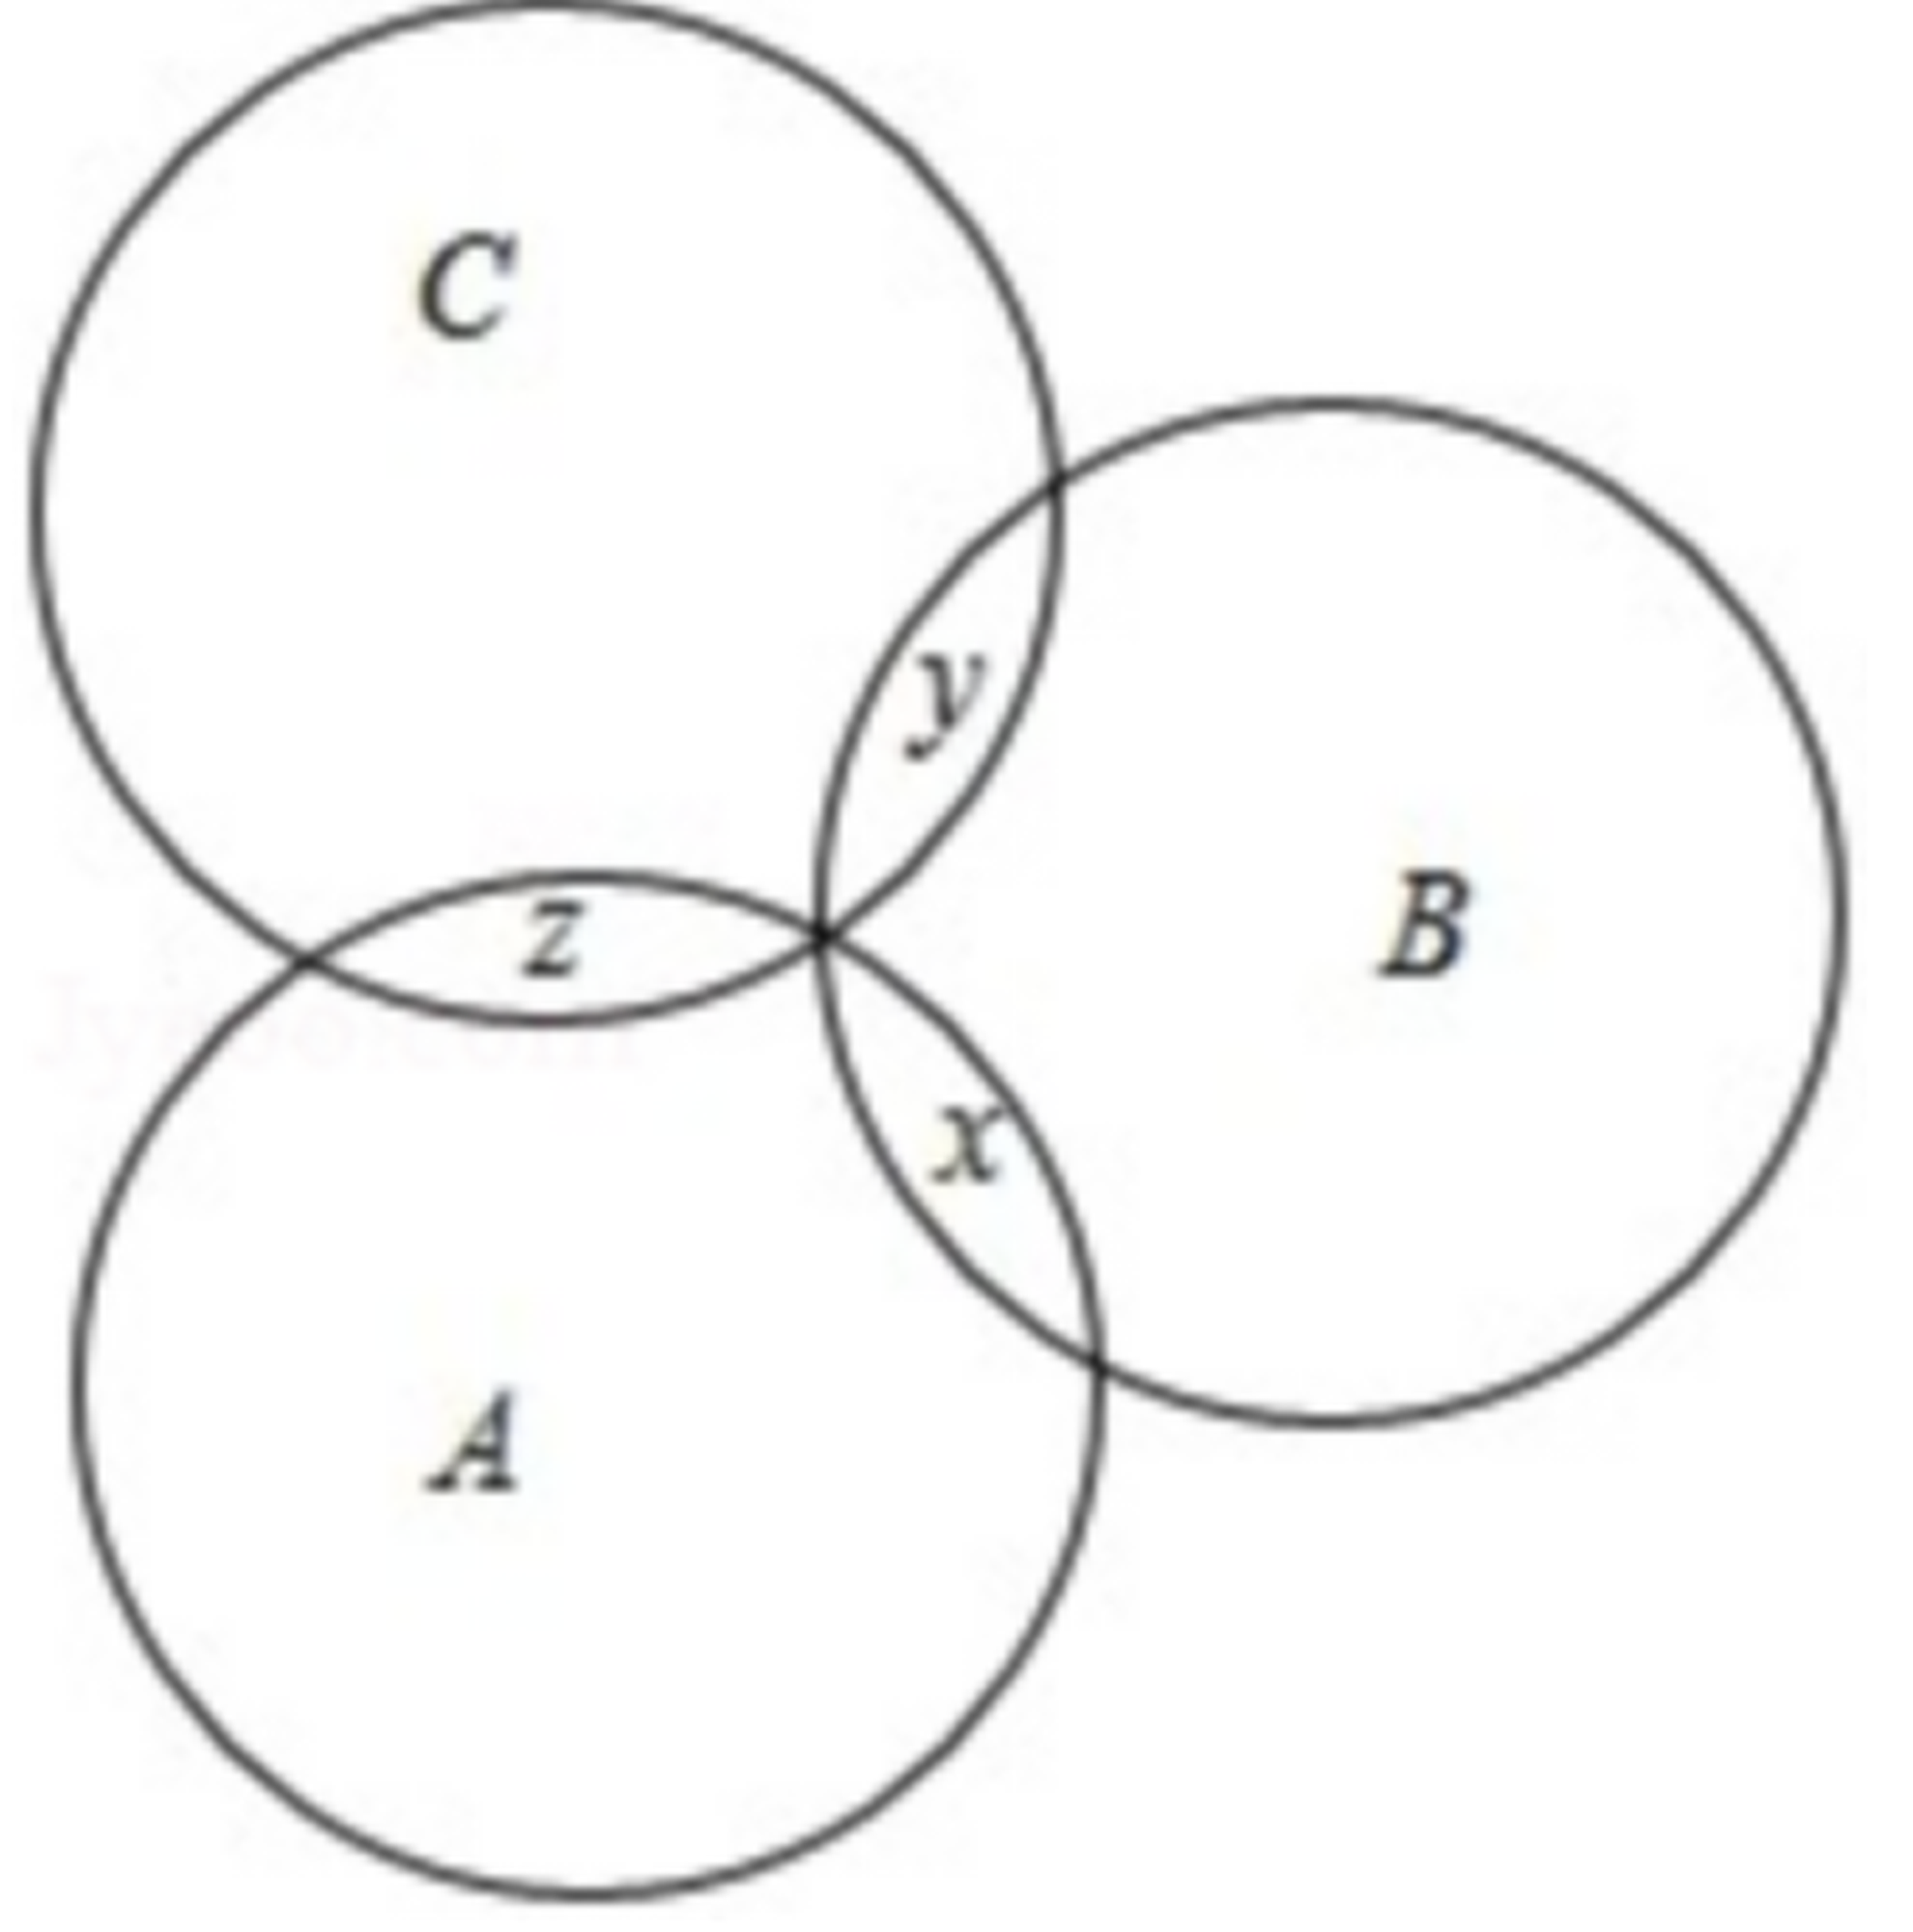
\includegraphics[width=0.30\textwidth]{figures/venn_ABC_x_y_z_h39.png}
\end{center}
\step{因为 $|A\cap B|=|B\cap C|=|C\cap A|=1$，且 $x$、$y$、$z\in\{1,2,3\}$，}
\step{所以集合 $A=\{x,z\}$，$B=\{x,y\}$，$C=\{z,y\}$，}
\step{若 $x=1$，$y=2$，$z=3$，则 $A=\{1,3\}$，$B=\{1,3\}$，$C=\{2,3\}$，}
\step{将 $1$，$2$，$3$ 进行全排列，有 $P_3^3=3\times2=6$ 个.}
\solend

\fi

\item 已知集合 $T=\{1,2,\cdots,2025\}$，对于 $T$ 的每一个非空子集的所有元素，计算它们乘积的倒数，
则所有这样倒数的和为 \blankline[4.4em].

\ans{$2025$}

\ifanswer
\solbegin
\step{集合 $T=\{1,2,\cdots,2025\}$ 的非空子集的个数为 $2^{2025}-1$，}
\step{这些子集中，每个元素的乘积分别为}
\step{$1,2,3,\cdots,2025,1\times2,1\times3,\cdots,1\times2025,\cdots,1\times2\times3\times\cdots\times2025$，}
\step{每项都可以看作是从 $1,2,3,\cdots,2025$ 中选择若干项的乘积，}
\step{$1+\dfrac12+\cdots+\dfrac{1}{2025}+\dfrac{1}{1\times2}+\dfrac{1}{1\times3}+\cdots+\dfrac{1}{2024\times2025}
+\cdots+\dfrac{1}{1\times2\times\cdots\times2025}$}
\step{$=(1+1)\left(1+\dfrac12\right)\cdots\left(1+\dfrac{1}{2025}\right)-1
=2\times\dfrac32\times\dfrac43\times\cdots\times\dfrac{2026}{2025}-1=2025$.}
\solend

\fi

% 第 24 题是压轴题，题干较长；试卷版在它之前量一次页高，尽量不与前文分家（照全稿成例）。
\ansneed{5cm}
% 注：原卷【解析】①③ 两步把 $f(x)$ 印作 $f[x[x]]$，显系笔误，照录未改，见文件头「笔误/存疑」⑦。
\item 若 $X$ 是一个集合，$T$ 是一个以 $X$ 的某些子集为元素的集合，且满足：①$X$ 属于 $T$，
$\varnothing$ 属于 $T$；②$T$ 中任意多个元素的并集属于 $T$；③$T$ 中任意多个元素的交集属于 $T$.
则称 $T$ 是集合 $X$ 上的一个拓扑. 已知函数 $f(x)=[x[x]]$，其中 $[x]$ 表示不大于 $x$ 的最大整数，
当 $x\in(0,n]$，$n\in\N^*$ 时，函数 $f(x)$ 值域为集合 $A_n$，则集合 $A_2$ 上的含有 $4$ 个元素的
拓扑 $T$ 的个数为 \blankline[4.4em].

\ans{$9$}

\ifanswer
\solbegin
\step{由题意，$n=2$，故 $0<x\leqslant2$，}
\step{①当 $0<x<1$ 时，则 $[x]=0$，所以 $f[x[x]]=0$，}
\step{②当 $x=1$ 时，$[x]=1$ 显然 $f(1)=1$，}
\step{③当 $1<x<2$ 时，$[x]=1$，所以 $f[x[x]]=[x]=1$，}
\step{④当 $x=2$ 时，$f(2)=4$，}
\step{所以 $A_2=\{0,1,4\}$，}
\step{因为 $T$ 中含有 $4$ 个元素，其中两个元素 $\varnothing$ 和 $A_2$，}
\step{$A_2=\{0,1,4\}$. 其它两个元素为 $A$、$B$，则
$\begin{cases}A\neq\varnothing\\ A\neq A_2\\ B\neq\varnothing\\ B\neq A_2\\ A\neq B\end{cases}$，}
\step{由对称性，不妨设 $1\leqslant|A|\leqslant|B|\leqslant2$，其中 $|A|$、$|B|$ 表示集合 $A$ 中元素的个数，}
\step{因为 $\begin{cases}A\cap B\in T\\ A\cup B\in T\end{cases}$，又 $|A|\leqslant|B|$，所以 $A\cap B=\varnothing$ 或 $A$，}
\step{若 $A\cap B=\varnothing$，则 $A\cup B$ 只能等于 $A_2$，}
\step{（若 $A\cup B=B$，则 $A\sub B$，则 $A\cap B=A=\varnothing$，矛盾）}
\step{则必有 $\begin{cases}|A|=1\\ |B|=2\end{cases}$，所以 $(A,B)$ 的个数 $\Leftrightarrow$ $A$ 的个数 $=3$ 种，}
\step{即 $\begin{cases}A=\{0\}\\ B=\{1,4\}\end{cases}$ 或 $\begin{cases}A=\{1\}\\ B=\{0,4\}\end{cases}$
或 $\begin{cases}A=\{4\}\\ B=\{0,1\}\end{cases}$；}
\step{若 $A\cap B=A\Leftrightarrow A\sub B$ 此时满足 $A\cup B=B$，}
\step{因为 $A\neq B$ 且 $1\leqslant|A|$ 且 $|B|\leqslant2$，所以 $\begin{cases}|A|=1\\ |B|=2\end{cases}$，}
\step{所以 $B$ 的选择共有 $C_3^2=3$ 种，则 $A$ 的个数有 $C_2^1$ 种，}
\step{所以 $(A,B)$ 的个数 $=2\times3=6$ 种.}
% 这六组「$A$／$B$」按原卷排作两行（前五个一行、第六个另起一行）；因五组并排时
% amsmath 的 cases 会为每组的第二列各留一枚 \quad，本行改排 \left\{\begin{matrix}…\end{matrix}\right.
% 以省下这枚 \quad（照 README「说明」记的高一07 成例），字形与 cases 相同。
\step{（这 $6$ 种是 $\left\{\begin{matrix}A=\{0\}\\ B=\{0,1\}\end{matrix}\right.$、
$\left\{\begin{matrix}A=\{1\}\\ B=\{0,1\}\end{matrix}\right.$、
$\left\{\begin{matrix}A=\{0\}\\ B=\{0,4\}\end{matrix}\right.$、
$\left\{\begin{matrix}A=\{4\}\\ B=\{0,4\}\end{matrix}\right.$、
$\left\{\begin{matrix}A=\{1\}\\ B=\{1,4\}\end{matrix}\right.$、}
\step{$\left\{\begin{matrix}A=\{4\}\\ B=\{1,4\}\end{matrix}\right.$）.}
\step{综上，$T$ 的个数为 $9$ 个.}
\solend

\fi

\end{enumerate}

\end{document}
"
% 紧凑版：xelatex "\def\iscompact{1}% 高一39_大同中学_周末作业4.1.tex
%   —— 高一上数学「2026-2027 年大同中学高一上周末作业 4.1」（试卷版/答案版）
% 试卷版：xelatex 高一39_大同中学_周末作业4.1.tex
% 答案版：xelatex "\def\isanswer{1}% 高一39_大同中学_周末作业4.1.tex
%   —— 高一上数学「2026-2027 年大同中学高一上周末作业 4.1」（试卷版/答案版）
% 试卷版：xelatex 高一39_大同中学_周末作业4.1.tex
% 答案版：xelatex "\def\isanswer{1}% 高一39_大同中学_周末作业4.1.tex
%   —— 高一上数学「2026-2027 年大同中学高一上周末作业 4.1」（试卷版/答案版）
% 试卷版：xelatex 高一39_大同中学_周末作业4.1.tex
% 答案版：xelatex "\def\isanswer{1}\input{高一39_大同中学_周末作业4.1.tex}"
% 紧凑版：xelatex "\def\iscompact{1}\input{高一39_大同中学_周末作业4.1.tex}"
%
% 原始材料是微信公众号图文（公众号「魔都数学加油站」连载「27学年高一 39」，署名「破晓」，
% 2026-09-26 21:29 发布，原文标题「27学年高一39——2026-2027年上海市大同中学高一上周末作业4.1」，
% 原文链接 https://mp.weixin.qq.com/s/HR2hIayXUXNi4zTs3PioiQ ），正文为 11 张 PNG 页。**同一篇里各页分辨率不一致**（2560×3620 与 4762×6735 两档混排：第 1、3、8、10 页为
% 2560×3620，第 2、4、5、6、7、9、11 页为 4762×6735）。原文本身就是一份**讲评版**——除第 15 题
% 外各题题下直接印【解析】（无单独的【答案】行），第 15 题的答案「D」直接印在题干末尾的括号内。
% 试题文字、答案与解析均照原卷录入，未改内容。卷面的粉色斜水印「魔都数学加油站」属水印，未录入。
%
% 卷首标题：原卷页首印作「2026-2027 年大同中学高一上周末作业 4.1」（**卷面标题行即带校名**，
% 年份区间按全稿惯例排 en dash，前缀照原卷保留「年」）。
%
% 篇幅与题号：卷面自「一、填空题」的**第 3 题**起编，终于「附加题」的**第 24 题**，共 22 题
% （填空 3—12、选择 13—16、解答 17—20、附加题 21—24）。第 1、2 题未在该文中发布——这是该
% 公众号连载讲评版的通例（高一02—高一09 等均自第 3 题起编，README「说明」已记），**不是截断**，
% 故本稿题号亦自 3 起。它与 高一40（大同中学 周末作业4.2）同属「周末作业 4」系列但**各自独立起编**
% （4.2 自第 3 题起、终于第 19 题），不是同一份试卷的两半。
%
% 与原卷的排版差异（均已在 README「说明」中交代）：
%   ① 原文自**第 3 题**起（第 1、2 题未在该文中发布），故本稿题号亦自 3 起，填空题以
%      \setcounter{enumi}{2} 起编；选择、解答、附加题三节各按上一节末号另设 \setcounter
%      （选择题 \setcounter{enumi}{12}、解答题 \setcounter{enumi}{16}、附加题 \setcounter{enumi}{20}）；
%   ② 原卷本就印有「一、填空题」「二、选择题」「三、解答题」三节标题，末节印作「附加题」
%      （**不带「四、」**，且题号 21—24 续前编、不另起），本稿照原卷分节，只把标题改排成全稿
%      统一的「大节标题」样式；
%   ③ 原卷是「讲评版」：除第 15 题外，各题题下均印【解析】（**全卷无一条独立的【答案】行**）；
%      第 15 题无解析，答案「D」直接印在题干末尾的括号内。本稿统一改为试卷版隐去、答案版以
%      \ans{}／\ifanswer 块给出，两版彻底分离；原卷写在【解析】末句的结果，本稿照 高一38
%      （同校同系列、同为讲评版）的成例另提为 \ans{}；
%   ④ 数集记号原卷两套并用：实数集作斜体的 $R$（第 7、11、14、17、18、19 题），整数集作斜体
%      $Z$（第 10 题），自然数集作斜体 $N$ 及 $N^*$（第 16、20、21、24 题），本稿按全稿惯例
%      统一写作 $\R$、$\Z$、$\N$、$\N^*$；
%   ⑤ 补集符号原卷两套并用：第 7 题作前缀式的 $C_U$（且题干称全集为 $I$，见「笔误/存疑」①），
%      第 14、15、18 题作上横线（$\overline{H}$、$\overline{A}$、$\overline{B}$），本稿照录、不归一
%      （前缀式写作 $\complement_U$，与 高一c／高一10 的成例一致）；
%   ⑥ 包含符号原卷两套并用：第 3 题作**无下划线**的 $\subset$，第 15、18、20、24 题作**带下划线**
%      的 $\sub$，本稿照录、不归一；
%   ⑦ 原卷填空的横线约两个字宽，本稿按全稿惯例统一排 \blankline[4.4em]；
%   ⑧ 第 7、11、22 题各有插图，取原卷截图、4× LANCZOS 放大（figures/venn_N_cap_CI_M_h39.png、
%      figures/plane_grid_4squares_h39.png、figures/venn_ABC_x_y_z_h39.png）；第 7 题的 Venn 属
%      **题干**（试卷版、答案版都出），第 11、22 题的图在【解析】内（仅答案版出）。第 7 题图
%      左下、第 11 题图的上／左／右边缘带进极淡的原卷粉色水印残影——照全稿「插图直接取自
%      原卷截图、不用 TikZ 重绘、不修图」的体例保留（再裁会切到坐标轴与 $x$、$y$、$O$ 标注）；
%   ⑨ 原卷并列的字母、数字（「$x_1,x_2$」「$a,b$」「$1,2,3,\cdots,11$」）多作半角逗号或不加标点，
%      本稿按全稿惯例改排顿号（$x_1$、$x_2$）或把数列并入行内公式；半角括号、逗号一律排全角，
%      数学式内部的标点照原样；
%   ⑩ 原卷未印副标题，本稿按**本卷实际内容**补出副标题「集合与常用逻辑用语」（依据见下条）。
%
% 副标题（\examtitlest 第二个参数）：本卷卷面未印副标题，由本稿补出，取值按 2026-09-26 起的
%   新口径「只用本卷实际内容的模块名」定为「集合与常用逻辑用语」。依据：全卷 22 题（第 3—24 题）中，
%   第 3、5、7、8、10、11、14、15、16、17、18、19、20、21、22、23、24 题共 17 题是集合的运算与
%   关系、子集／真子集、补集、集合新定义（「全食／偏食」、最小相交、拓扑、特征数）与集合计数，
%   以及命题与常用逻辑用语（第 3 题充要条件、第 5 题存在量词命题、第 17 题命题真假）；其余两题
%   第 4、6 考一元二次方程的根（韦达定理）与方程恒等，第 9、12、13 题是不等式（一元二次不等式组
%   的整数解、一元二次不等式解集、不等式的性质）——不等式合计 3/22，**不足全卷三分之一**，
%   故不并标「不等式」。
%
% 原卷笔误/存疑（均照抄原卷、未改，见源码中该处上方注释）：
%   ① 第 7 题题干称「全集 $I=R$」，而【解析】两处把补集写作 $C_U M$（下标作 $U$），前后记号不一；
%      本稿照录，未改；
%   ② 第 4 题【解析】两处把判别式印作 $\triangle=[2(m-1)^2-16m^2]$（方括号内首项漏了平方，
%      正确应作 $[2(m-1)]^2-16m^2$）；按其所判「$m=\frac12$ 时 $<0$、$m=-\frac12$ 时 $>0$」反推，
%      $[2(m-1)]^2-16m^2$ 在 $m=\frac12$ 时为 $-3<0$、在 $m=-\frac12$ 时为 $5>0$，与结论一致；
%      本稿照录；
%   ③ 第 9 题【解析】把方程组第二式印作 $1-2<-k\leqslant3$，按其结论 $-3\leqslant k<2$ 反推，
%      疑当作 $-2<-k\leqslant3$（原卷多一个「$1$」）；本稿照录；
%   ④ 第 17 题【解析】首句「由数 $y=-x^2+ax-1=-x+3$」中的「由数」显系「由」或「由函数」之误；
%      且末段「若 $p$ 真 $q$ 假…得 $a\in R$」「若 $p$ 假 $q$ 真…此时 $a$ 无解」与结论「$a$ 的取值范围
%      是 $R$」自相矛盾（按 $p:a\leqslant-5$、$q:a>-6$，$p$ 真 $q$ 假应为 $a\leqslant-6$，$p$ 假 $q$ 真
%      应为 $a>-5$，合起来是 $a\leqslant-6$ 或 $a>-5$，并非 $R$）；本稿一律照录，未按正确解法改写；
%   ⑤ 第 18 题【解析】(2) 把 $B=\{x\mid x^2+a\leqslant0\}$（$a<0$）印作右端开的
%      $\{x\mid-\sqrt{-a}\leqslant x<\sqrt{-a}\}$（应为闭的「$\leqslant$」）；按其所判
%      $\sqrt{-a}<\frac12$ 反推，不影响结论；本稿照录；
%   ⑥ 第 22 题【解析】在 $x=1$、$y=2$、$z=3$ 时把 $B=\{x,y\}$ 印作 $\{1,3\}$（应为 $\{1,2\}$），
%      与本行前面「$B=\{x,y\}$」不合；本稿照录；
%   ⑦ 第 24 题【解析】①③ 两步把 $f(x)$ 印作 $f[x[x]]$，显系笔误；本稿照录。
%   ⑧ 第 8 题【解析】「即方程 $x^2+ax+b=x$，$x^2+(a-1)x+b=0$ **由**两个相等的实数根为 $4$」——
%      「由」当为「有」（「设…是…有」的杂糅）；本稿照录；
%   ⑨ 第 10 题：题设 $a\oplus b=b(a^2+b^2+1)$，而集合定义里含 $\dfrac{a\oplus b}{2b}$；$-2<a<b<2$、
%      $a$、$b\in\Z$ 时 $(a,b)=(-1,0)$ 也合条件、却使分母 $2b=0$，原卷解析仍代入该组并约去
%      $b$ 得 $x=1$（答案集恰好不变）；本稿照录；
%   ⑩ 第 15 题选项列里 ② 与 ③ 之间**漏排分隔号**（原卷作「② $\overline{A}\cap B=\varnothing$③
%      $\overline{A}\sub\overline{B}$；」——①、③ 后都有「；」，② 后没有）；本稿照录；
%   ⑪ 第 20(2) 把 $\{1,2,\cdots,20\}$ 分成的 11 个集合里，$\{8,11\}$ 与 $\{9,12\}$ 之间误用
%      **句号**「.」（同行其余处皆逗号）；本稿照录；
%   ⑫ 第 20(3)① 推理不严：原卷写「选 5 则不选 1、9；选 6 则不选 2、10；选 7 则不选 3、11；
%      则只剩 4、8」——但 4 与 8 相差 $4$、不能同选，该情形实际最多只能取 $4$ 个；末句结论
%      「不超过 $5$ 个」仍成立；本稿照录；
%   ⑬ 第 16 题【解析】两种下标并存：「所以在 $A_i$ 的特征数构成中」原卷作斜体 $A_i$，而
%      「要使 $X_1+X_2+X_3$ 最大（小），则（应）在集合 $A_1$ 中首先放置…」两处原卷作
%      **数字 $1$**（与同句 $X_1$ 的角标同形）；本稿照录、未归一。
%
% 图取原卷截图（依次见各处的 \includegraphics 前的注释），4× LANCZOS 放大。
\documentclass[a4paper,11pt]{article}
\usepackage{common}

\begin{document}

\examtitlest[3]{2026--2027 年大同中学高一上周末作业 4.1}{集合与常用逻辑用语}

\bigsec{一、填空题}

\begin{enumerate}
\setcounter{enumi}{2}

\item “$x\geqslant a$”是“$0<x<2$”的必要非充分条件，则实数 $a$ 的取值范围是 \blankline[4.4em].

\ans{$(-\infty,0]$}

\ifanswer
\solbegin
\step{因为 $x\geqslant a$ 是 $0<x<2$ 的必要非充分条件，所以 $(0,2)\subset[a,+\infty)$，所以 $a\leqslant0$，}
\step{则实数 $a$ 的取值范围是 $(-\infty,0]$.}
\solend

\fi

% 注：原卷$[2(m-1)^2-16m^2]$ 首项漏了平方（应为 $[2(m-1)]^2-16m^2$），照录未改，见文件头「笔误/存疑」②。
\item 若关于 $x$ 的方程 $x^2+2(m-1)x+4m^2=0$ 有两个实数根，且这两根互为倒数，则 $m=$ \blankline[4.4em].

\ans{$-\dfrac12$}

\ifanswer
\solbegin
\step{设 $x_1$、$x_2$ 是方程 $x^2+2(m-1)x+4m^2=0$ 有两个实数根，}
\step{则 $x_1x_2=4m^2=1$，解得 $m=\dfrac12$ 或 $m=-\dfrac12$，}
\step{又当 $m=\dfrac12$ 时，$\triangle=[2(m-1)^2-16m^2]<0$，舍去，}
\step{当 $m=-\dfrac12$ 时，$\triangle=[2(m-1)^2-16m^2]>0$，故 $m=-\dfrac12$.}
\solend

\fi

\item 已知命题：“存在 $x\in[1,2]$，使 $x^2+2x+a\geqslant0$”为真命题，则 $a$ 的取值范围是 \blankline[4.4em].

\ans{$a\geqslant-8$}

\ifanswer
\solbegin
\step{若存在 $x\in[1,2]$，使 $x^2+2x+a\geqslant0$，}
\step{则等价为存在 $x\in[1,2]$，使 $x^2+2x\geqslant-a$，}
\step{当存在 $x\in[1,2]$ 时，设 $y=x^2+2x=(x+1)^2-1$，则 $3\leqslant y\leqslant8$，}
\step{所以要使 $x^2+2x\geqslant-a$，则 $8\geqslant-a$，即 $a\geqslant-8$.}
\solend

\fi

\item 已知方程 $a(3x+2)+b(2x-3)=8x+3$ 有无穷多个解，则 $a:b=$ \blankline[4.4em].

\ans{$30:7$}

\ifanswer
\solbegin
\step{$a(3x+2)+b(2x-3)=(3a+2b)x+2a-3b=8x+3$ 有无穷多个解，}
\step{所以 $\begin{cases}3a+2b=8\\ 2a-3b=3\end{cases}$，解得 $a=\dfrac{30}{13}$，$b=\dfrac{7}{13}$，所以 $a:b=30:7$.}
\solend

\fi

% 注：原卷题干称「全集 $I=R$」，而【解析】两处把补集写作 $C_U M$（下标作 $U$），前后记号不一；
%     照录未改，见文件头「笔误/存疑」①。
\item 已知集合 $M=\{x\mid y=\sqrt{3-x^2}\}$，$N=\{x\mid-3\leqslant x\leqslant1\}$，全集 $I=\R$，
则图中阴影部分表示的集合为 \blankline[4.4em].

% 图取原卷截图（01.png，2560×3620）右栏，4× LANCZOS 放大。
\begin{center}
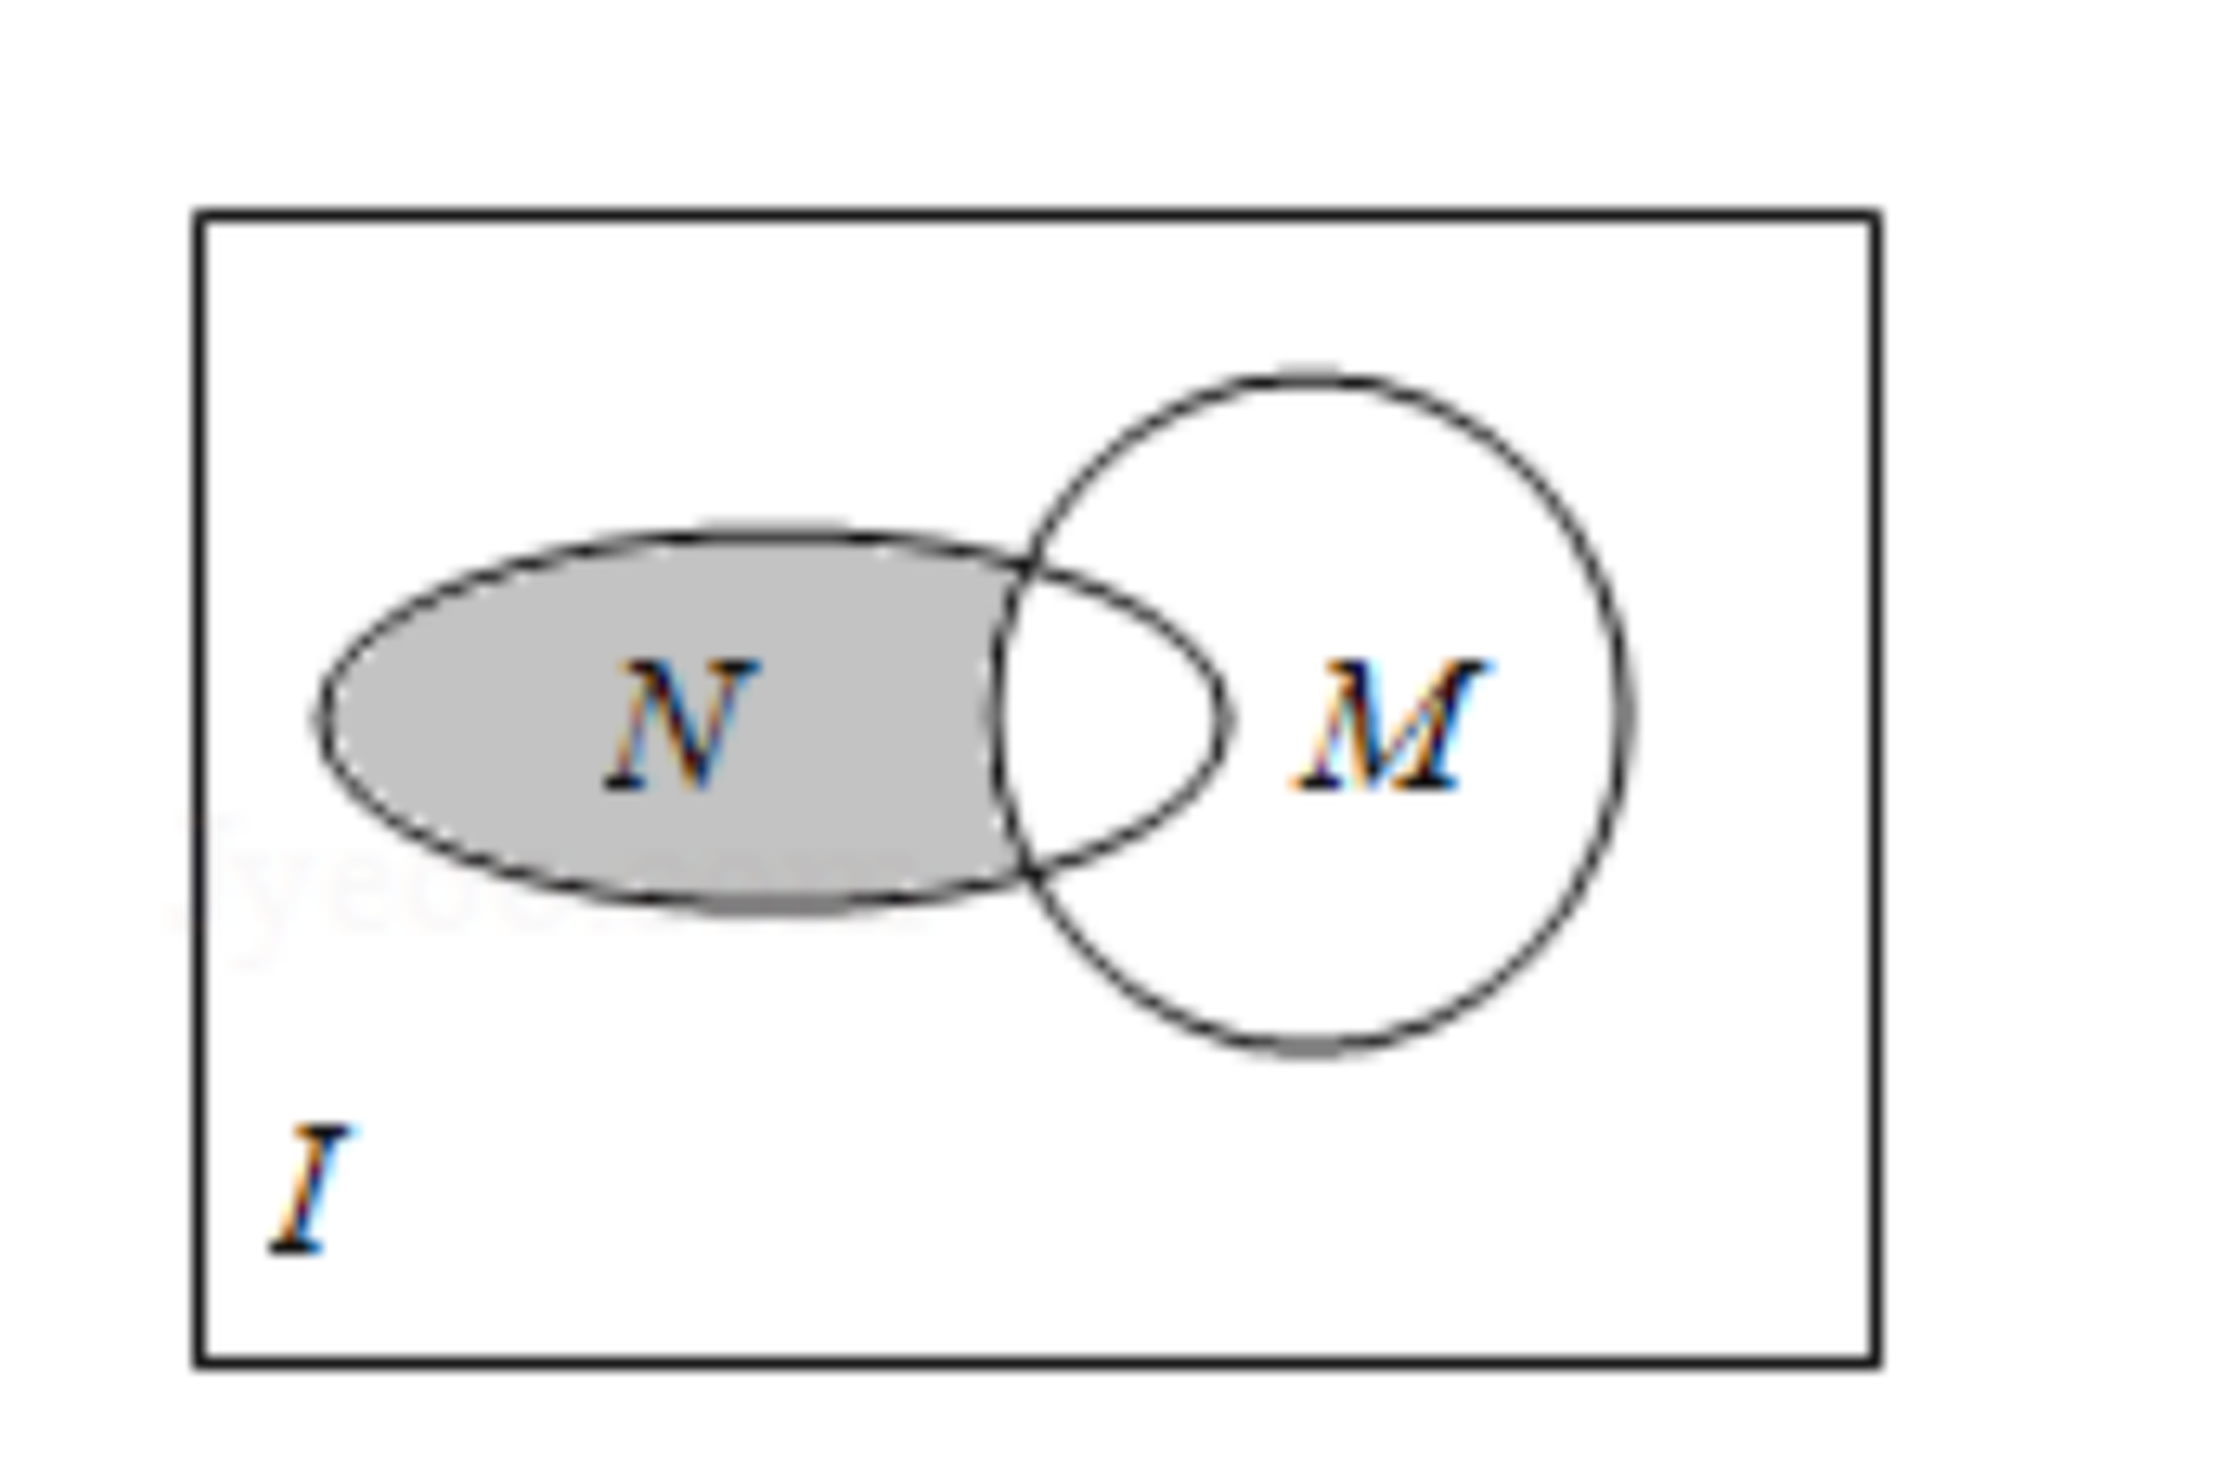
\includegraphics[width=0.30\textwidth]{figures/venn_N_cap_CI_M_h39.png}
\end{center}

\ans{$[-3,-\sqrt3)$}

\ifanswer
\solbegin
\step{阴影部分用集合表示为 $N\cap(\complement_UM)$.}
\step{则 $M=\{x\mid y=\sqrt{3-x^2}\}=\{x\mid3-x^2\geqslant0\}=\{x\mid-\sqrt3\leqslant x\leqslant\sqrt3\}$，}
\step{则 $\complement_UM=\{x\mid x>\sqrt3\text{ 或 }x<-\sqrt3\}$，$N=\{x\mid|x+1|\leqslant2\}=\{x\mid-3\leqslant x\leqslant1\}$，}
\step{则 $N\cap(\complement_UM)=\{x\mid-3\leqslant x<-\sqrt3\}$.}
\solend

\fi

\item 已知 $f(x)=x^2+ax+b$，集合 $\{x\mid f(x)=x\}=\{4\}$，将集合 $M=\{x\mid f(x)=4\}$ 用列举法表示 \blankline[4.4em].

\ans{$\{3,4\}$}

\ifanswer
\solbegin
\step{已知 $f(x)=x^2+ax+b$，集合 $\{x\mid f(x)=x\}=\{4\}$，}
% 注：原卷本行作「…$x^2+(a-1)x+b=0$ **由**两个相等的实数根为 $4$」——「由」当为「有」
%     （「设…是…有」的杂糅）；本稿照录未改，见文件头「原卷笔误/存疑」⑧。
\step{即方程 $x^2+ax+b=x$，$x^2+(a-1)x+b=0$ 由两个相等的实数根为 $4$，}
\step{所以 $\triangle=(a-1)^2-4b=0$，即 $x^2+(a-1)x+b=(x-4)^2$，所以 $b=16$，$a=-7$，}
\step{所以 $f(x)=x^2+ax+b=x^2-7x+16$，所以集合 $M=\{x\mid f(x)=4\}$，}
\step{即 $x^2-7x+16=4$，$x^2-7x+12=0$，故 $M=\{x\mid f(x)=4\}=\{3,4\}$.}
\solend

\fi

% 注：原卷方程组第二式印作 $1-2<-k\leqslant3$，按其结论 $-3\leqslant k<2$ 反推疑当作 $-2<-k\leqslant3$，
%     照录未改，见文件头「笔误/存疑」③。
\item 关于 $x$ 的不等式组 $\begin{cases}x^2-x-2>0\\ 2x^2+(2k+5)x+5k<0\end{cases}$ 的整数解的集合为 $\{-2\}$，
则实数 $k$ 的取值范围 \blankline[4.4em].

\ans{$-3\leqslant k<2$}

\ifanswer
\solbegin
\step{原不等式组即 $\begin{cases}(x-2)(x+1)>0\\ (x+k)(2x+5)<0\end{cases}$，整数解的集合为 $A$，若 $A=\{-2\}$，}
\step{则 $(-2+k)(2\times(-2)+5)<0$，所以 $k<2$，且有 $\begin{cases}-k>-\dfrac52\\ 1-2<-k\leqslant3\end{cases}$，}
\step{解得 $-3\leqslant k<2$.}
\solend

\fi

\item 规定 $\oplus$ 与 $\otimes$ 是两个运算符号，其运算法则如下，对任意实数 $a$、$b$ 有：$a\otimes b=ab$，
$a\oplus b=b(a^2+b^2+1)$. 若 $-2<a<b<2$ 且 $a$、$b\in\Z$，
$A=\left\{x\mid x=2(a\otimes b)+\dfrac{a\oplus b}{2b}\right\}$，则用列举法表示集合 $A=$ \blankline[4.4em].

\ans{$\left\{1,-\dfrac12\right\}$}

\ifanswer
\solbegin
\step{$A=\left\{x\mid x=2(a\otimes b)+\dfrac{a\oplus b}{2b}\right\}
=\left\{x\mid x=2ab+\dfrac{b(a^2+b^2+1)}{2b}\right\}$}
\step{$=\left\{x\mid x=2ab+\dfrac12a^2+\dfrac12b^2+\dfrac12\right\}
=\left\{x\mid x=\dfrac12(a+b)^2+ab+\dfrac12\right\}$，}
% 注：题设含 $\dfrac{a\oplus b}{2b}$，而 $-2<a<b<2$、$a$、$b\in\Z$ 时 $(a,b)=(-1,0)$ 也合条件、
%     却使分母 $2b=0$；原卷解析仍代入该组并约去 $b$ 得 $x=1$（答案集恰好不变）。本稿照录，
%     见文件头「原卷笔误/存疑」⑨。
\step{当 $a=-1$，$b=0$ 时，$x=1$；当 $a=-1$，$b=1$ 时，$x=-\dfrac12$；}
\step{当 $a=0$，$b=1$ 时，$x=1$；所以 $A=\left\{1,-\dfrac12\right\}$.}
\solend

\fi

\item 高斯是德国著名的数学家，近代数学奠基者之一，享有“数学王子”的称号，为了纪念数学家高斯，
我们把取整函数 $y=[x]$，$x\in\R$ 称为高斯函数，其中 $[x]$ 表示不超过 $x$ 的最大整数，
如 $[1.1]=1$，$[-1.1]=-2$. 则点集 $P=\{(x,y)\mid[x]^2+[y]^2=1\}$
所表示的平面区域的面积是 \blankline[4.4em].

\ans{$4$}

\ifanswer
\solbegin
\step{$[x]^2+[y]^2=1$ 由 $\begin{cases}[x]=0\\ [y]=-1\end{cases}$ 或 $\begin{cases}[x]=0\\ [y]=1\end{cases}$
或 $\begin{cases}[x]=-1\\ [y]=0\end{cases}$ 或 $\begin{cases}[x]=1\\ [y]=0\end{cases}$ 四个平面区域组成，}
\step{即 $\begin{cases}0\leqslant x<1\\ -1\leqslant y<0\end{cases}$ 或 $\begin{cases}0\leqslant x<1\\ 1\leqslant y<2\end{cases}$
或 $\begin{cases}-1\leqslant x<0\\ 0\leqslant y<1\end{cases}$ 或 $\begin{cases}1\leqslant x<2\\ 0\leqslant y<1\end{cases}$，}
\step{作出平面区域如图所示，平面区域由四个边长为 $1$ 的正方形组成，}
% 图在【解析】内（仅答案版出），取原卷截图（03.png，2560×3620）中部，4× LANCZOS 放大。
\begin{center}
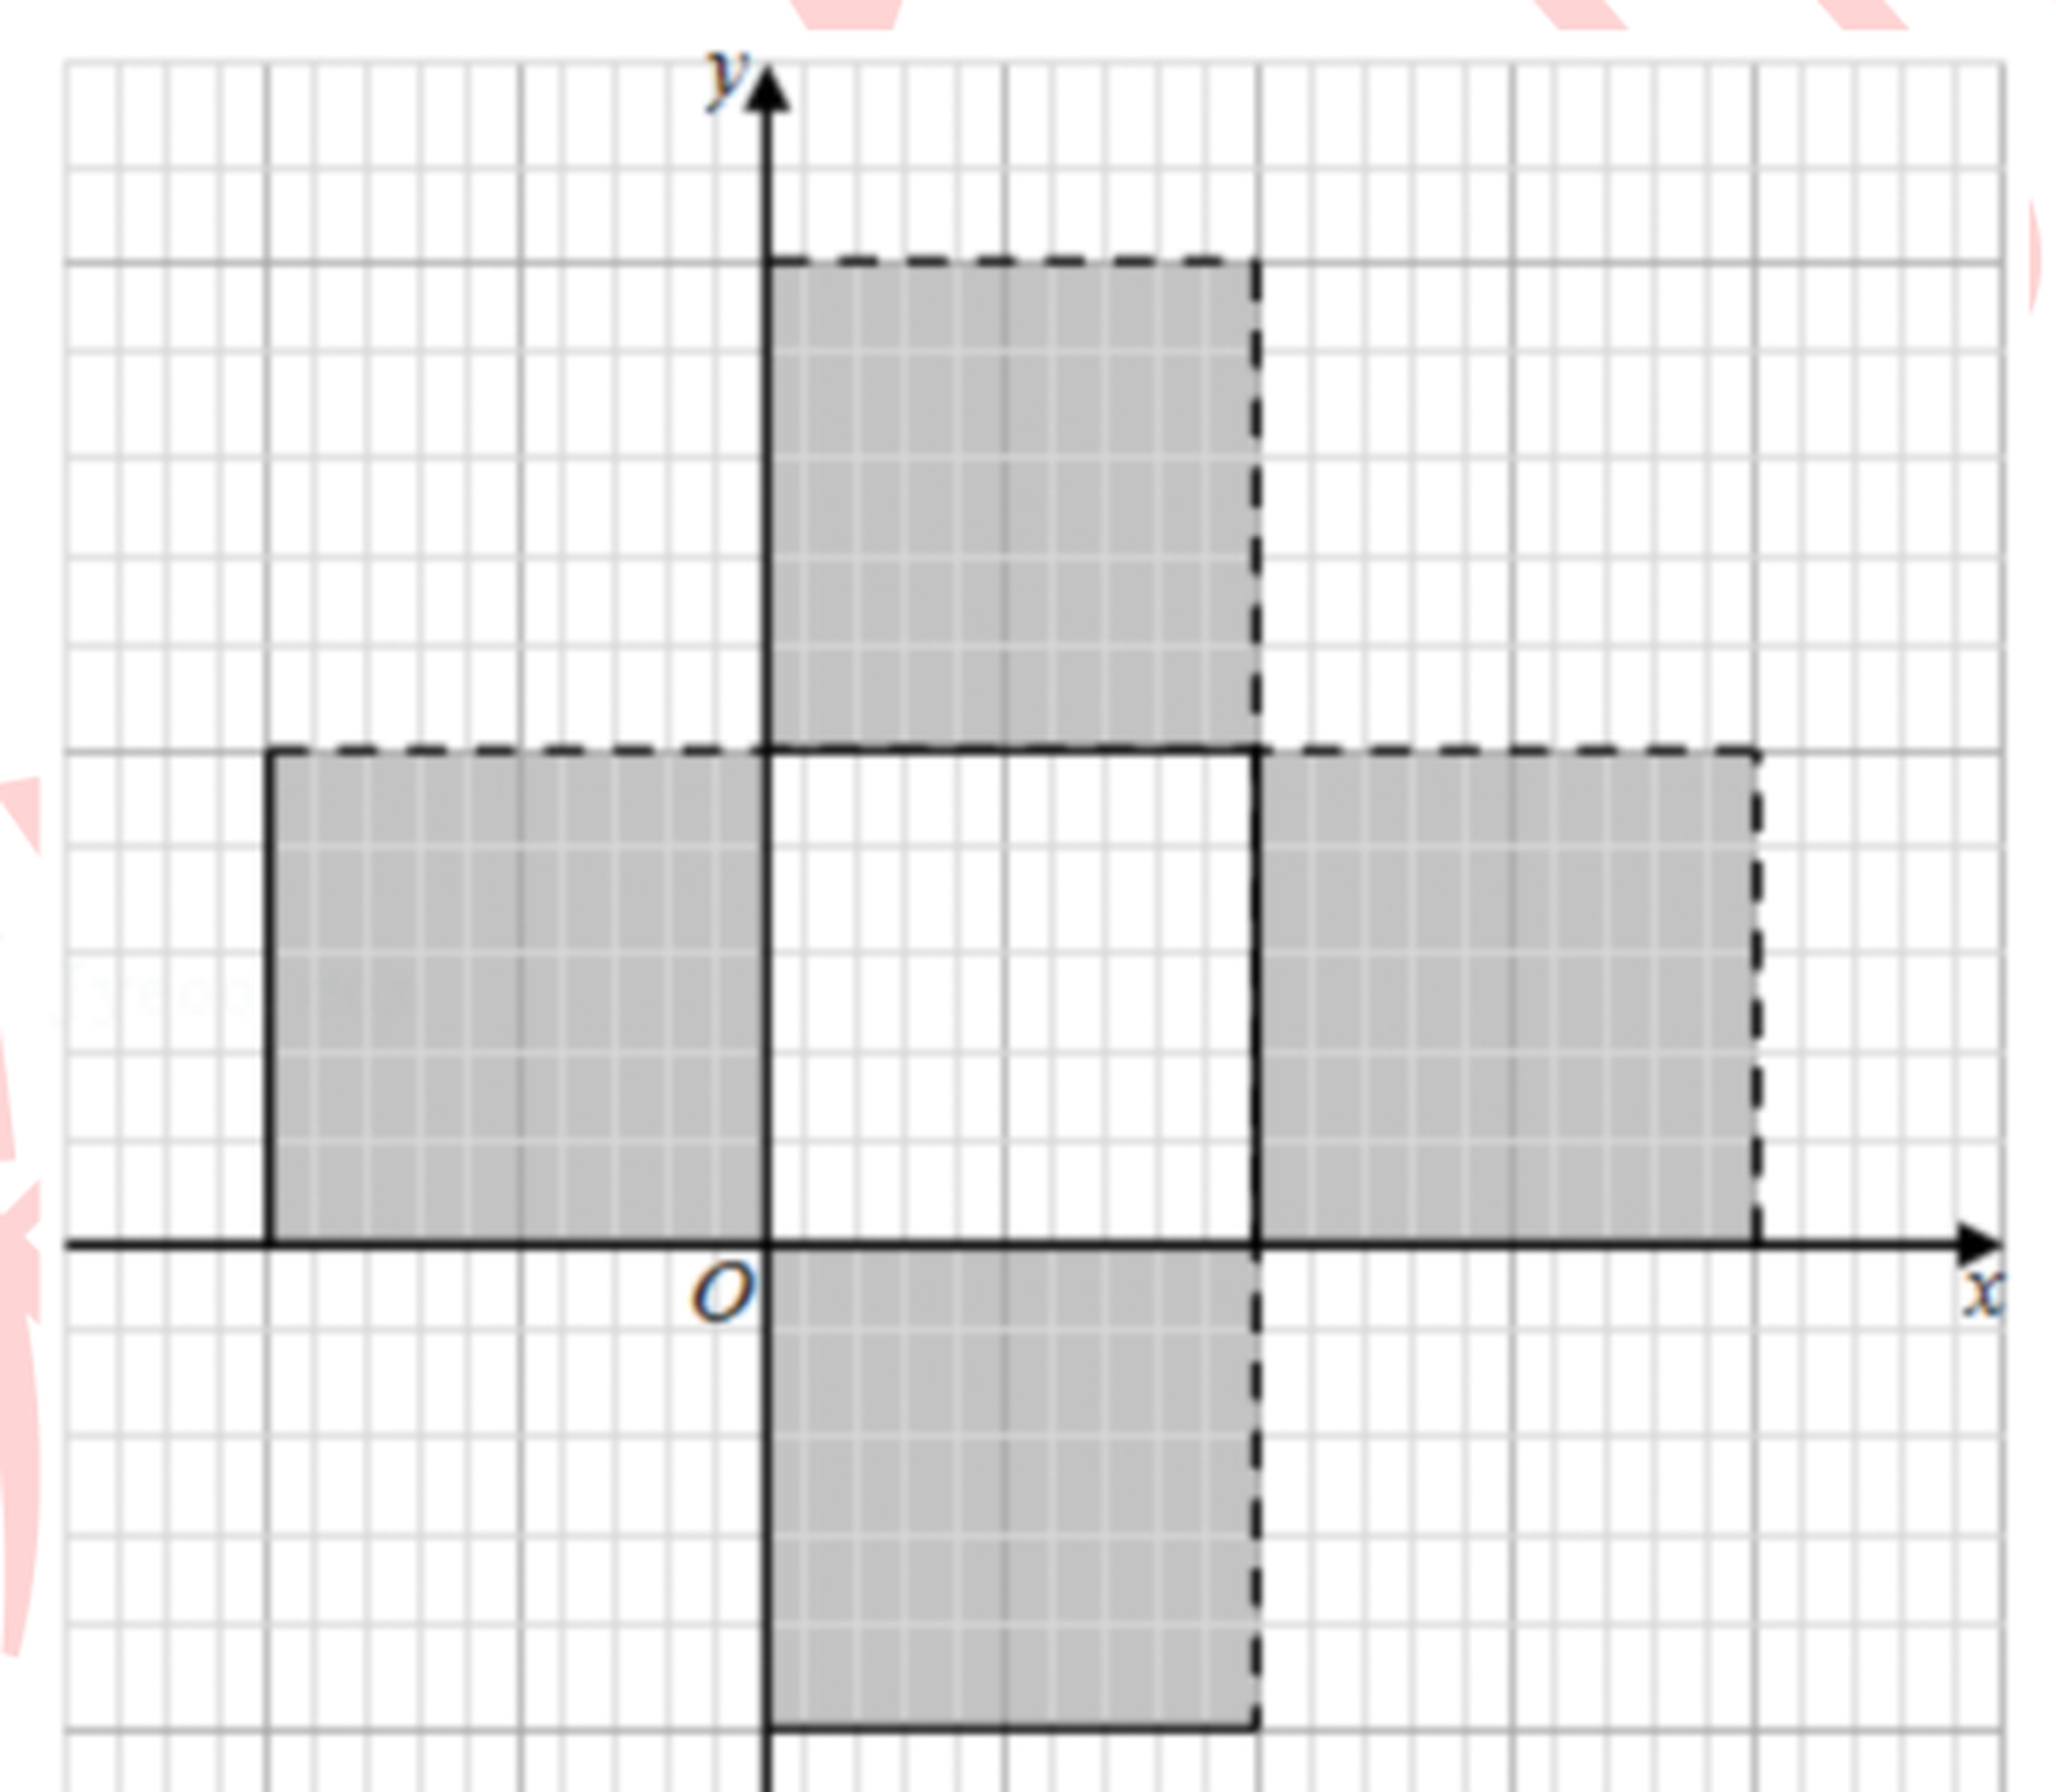
\includegraphics[width=0.38\textwidth]{figures/plane_grid_4squares_h39.png}
\end{center}
\step{总面积为 $1\times4=4$.}
\solend

\fi

\item 关于 $x$ 的不等式 $ax^2+bx+c>0$ 的解集为 $\{x\mid x<\beta\text{ 或 }x>\gamma\}(0<\beta<\gamma)$，
则不等式 $a(x^2+1)+b(x-1)+c>2ax$ 的解集为 \blankline[4.4em].

\ans{$(-\infty,\beta+1)\cup(\gamma+1,+\infty)$}

\ifanswer
\solbegin
\step{由题意得 $\beta$、$\gamma$ 为方程 $ax^2+bx+c=0$ 的两根且 $a>0$，}
\step{则 $\beta+\gamma=-\dfrac ba$，$\beta\gamma=\dfrac ca$，故 $b=-a(\beta+\gamma)$，$c=\beta\gamma a$，}
\step{则不等式可化为 $a(x^2+1)-a(\beta+\gamma)(x-1)+\beta\gamma a>2ax$，}
\step{因为 $a>0$，所以 $x^2+1-(\beta+\gamma)(x-1)+\beta\gamma>2x$，}
\step{即 $x^2-(\beta+\gamma+2)x+(\beta+\gamma+\beta\gamma+1)>0$，所以 $(x-\beta-1)(x-\gamma-1)>0$，}
\step{解得 $x<\beta+1$ 或 $x>\gamma+1$，所以不等式解集为 $(-\infty,\beta+1)\cup(\gamma+1,+\infty)$.}
\solend

\fi

\end{enumerate}

\bigsec{二、选择题}

\begin{enumerate}
\setcounter{enumi}{12}

\item 设 $a<b<0$，则下列不等式中不成立的是\mbox{（\quad）}

\keepwithprev
A. $\dfrac1a>\dfrac1b$\qquad B. $\dfrac{1}{a-b}>\dfrac1a$\qquad C. $|a|>-b$\qquad D. $\sqrt{-a}>\sqrt{-b}$

\ans{$B$}

\ifanswer
\solbegin
\step{令 $a=-2$，$b=-1$，}
\step{A、$-\dfrac12>-1$，正确；B、$-1<-\dfrac12$，故 B 错误；C、$2>1$，正确；}
\step{D、$\sqrt2>1$，正确；故选 B.}
\solend

\fi

\item 设实数集 $\R$ 为全集，集合 $P=\{x\mid f(x)=0\}$，$Q=\{x\mid g(x)=0\}$，$H=\{x\mid h(x)=0\}$，
则方程 $\dfrac{f^2(x)+g^2(x)}{h(x)}=0$ 的解集是\mbox{（\quad）}

\keepwithprev
A. $P\cap Q\cap\overline{H}$\qquad B. $P\cap Q$\qquad C. $P\cap Q\cap H$\qquad D. $P\cap Q\cup H$

\ans{$A$}

\ifanswer
\solbegin
\step{方程 $\dfrac{f^2(x)+g^2(x)}{h(x)}=0$ 等价于 $\begin{cases}f(x)=0\\ g(x)=0\\ h(x)\neq0\end{cases}$，}
\step{又因为 $P=\{x\mid f(x)=0\}$，$Q=\{x\mid g(x)=0\}$，$H=\{x\mid h(x)=0\}$，}
\step{所以方程 $\dfrac{f^2(x)+g^2(x)}{h(x)}=0$ 的解集是 $P\cap Q\cap\overline{H}$，故选 A.}
\solend

\fi

\item 设全集 $U$，在下列条件中，是 $B\sub A$ 的充要条件的有\mbox{（\quad）}

\keepwithprev
% 注：原卷此行 ② 与 ③ 之间**漏排分隔号**（①、③ 后都有「；」，② 后没有）；
%     本稿照录未补，见文件头「原卷笔误/存疑」⑩。
①$A\cup B=A$；\qquad ②$\overline{A}\cap B=\varnothing$\qquad ③$\overline{A}\sub\overline{B}$；\qquad ④$A\cup\overline{B}=U$

\keepwithprev
A. $1$ 个\qquad B. $2$ 个\qquad C. $3$ 个\qquad D. $4$ 个

\ans{$D$}

\item 已知集合 $M=\{x\mid x\in\N,0<x\leqslant15\}$，$A_1$、$A_2$、$A_3$ 满足：①$A_1\cup A_2\cup A_3=M$；
②每个集合都恰有 $5$ 个元素. 集合 $A_i(i=1,2,3)$ 中最大元素与最小元素之和称为 $A_i$ 的特征数，
记为 $X_i(i=1,2,3)$，则 $X_1+X_2+X_3$ 的值不可能为\mbox{（\quad）}

\keepwithprev
A. $37$\qquad B. $39$\qquad C. $48$\qquad D. $57$

\ans{$A$}

\ifanswer
\solbegin
\step{因为集合 $M=\{x\mid x\in\N,0<x\leqslant15\}=\{1,2,3,\cdots,15\}$，}
\step{又因为集合 $A_1$、$A_2$、$A_3$ 中，每个集合恰有 $5$ 个元素，}
\step{且 $A_1\cup A_2\cup A_3=M$ 有 $15$ 个元素，所以集合 $A_1$、$A_2$、$A_3$ 中没有重复元素，}
\step{因为 $1$ 是集合 $M$ 中数值最小的元素，$15$ 是集合 $M$ 中数值最大的元素，}
\step{所以在 $A_i$ 的特征数构成中，必有 $1$ 和 $15$，不妨设 $1\in A_1$，$15\in A_1$，}
% 注：原卷本行（与下面「最小」那句）在「集合」后的角标是**数字 $1$**（同句 $X_1$ 的角标同形），
%     而非上一行「$A_i$ 的特征数构成」里的斜体 $A_i$——原卷两种下标并存，本稿照录、不归一，
%     见文件头「原卷笔误/存疑」⑬。
\step{要使 $X_1+X_2+X_3$ 最大，则应该在集合 $A_1$ 中首先放置数值较小的元素，}
\step{即 $A_1=\{1,2,3,4,15\}$，所以 $5$ 与 $14$ 是剩下元素中数值最小或最大的元素，}
\step{同理，不妨设 $5\in A_2$，$14\in A_2$，接着在 $A_2$ 中再次放置数值较小的元素，}
\step{即 $A_2=\{5,6,7,8,14\}$，则 $A_3=\{9,10,11,12,13\}$，}
\step{此时 $X_1+X_2+X_3$ 有最大值为 $1+15+5+14+9+13=57$，}
\step{即 $X_1+X_2+X_3\leqslant57$；}
% 注：同上一处——原卷此行角标是**数字 $1$**（$A_1$），本稿照录，未与「$A_i$」归一。
\step{要使 $X_1+X_2+X_3$ 最小，则在集合 $A_1$ 中首先放置数值较大的元素，}
\step{即 $A_1=\{1,12,13,14,15\}$，所以 $2$ 与 $11$ 是剩下元素中数值最小或最大的元素，}
\step{同理，不妨设 $2\in A_2$，$11\in A_2$，接着在 $A_2$ 中再次放置数值较大的元素，}
\step{即 $A_2=\{2,8,9,10,11\}$，则 $A_3=\{3,4,5,6,7\}$，}
\step{此时 $X_1+X_2+X_3$ 有最小值为 $1+15+2+11+3+7=39$，}
\step{即 $X_1+X_2+X_3\geqslant39$，}
\step{综上，$39\leqslant X_1+X_2+X_3\leqslant57$，故选 A.}
\solend

\fi

\end{enumerate}

\bigsec{三、解答题}

\begin{enumerate}
\setcounter{enumi}{16}

% 注：原卷首句「由数 $y=-x^2+ax-1=-x+3$」中的「由数」显系「由」或「由函数」之误；末段
%     的两处分类讨论与结论自相矛盾（详见文件头「笔误/存疑」④）。本稿一律照录，未改。
\item 命题 $p$：函数 $y=-x^2+ax-1$ 与 $y=-x+3$ 图象交点的横坐标均为负值，
命题 $q$：关于 $x$ 的方程 $2(1-x)a+(x^2-10x-3)=0$ 的两个根，一个大于 $3$，另一个小于 $3$；
若命题 $p$ 和命题 $q$ 中有且仅有一个是真命题，求 $a$ 的取值范围.

\ans{$\R$}

\ifanswer
\solbegin
\step{由数 $y=-x^2+ax-1=-x+3$ 得 $x^2-(a+1)x+4=0$，}
\step{若横坐标均为负值，则满足 $\begin{cases}\Delta=(a+1)^2-16\geqslant0\\ x_1x_2=4>0\\ x_1+x_2=a+1<0\end{cases}$
得 $\begin{cases}a\geqslant3\text{ 或 }a\leqslant-5\\ a<-1\end{cases}$，得 $a\leqslant-5$，}
\step{即 $p:a\leqslant-5$，}
\step{若方程 $2(1-x)a+(x^2-10x-3)=0$ 的两个根，一个大于 $3$，另一个小于 $3$；}
\step{设 $f(x)=2(1-x)a+(x^2-10x-3)$，则 $f(3)<0$，即 $-4a-24<0$，}
\step{得 $a>-6$，即 $q:a>-6$，}
\step{因为命题 $p$ 和命题 $q$ 中有且仅有一个是真命题，}
\step{若 $p$ 真 $q$ 假，则 $\begin{cases}a\leqslant-5\\ a>-6\end{cases}$，得 $a\in\R$，}
\step{若 $p$ 假 $q$ 真，则 $\begin{cases}a>-5\\ a\leqslant-6\end{cases}$，此时 $a$ 无解，}
\step{综上，实数 $a$ 的取值范围是 $\R$.}
\solend

\fi

\ansspace[8]

\item 设全集是实数集 $\R$，$A=\left\{x\mid\dfrac{1-2x}{x-3}\geqslant0\right\}$，$B=\{x\mid x^2+a\leqslant0\}$.

\begin{enumerate}[label=(\arabic*)]

\item 当 $a=-4$ 时，求 $A\cup B$；

\item 若 $\overline{A}\cap B=B$，求实数 $a$ 的取值范围.

\end{enumerate}

\ans{（1）$\{x\mid-2\leqslant x<3\}$；（2）$\left(-\dfrac14,+\infty\right)$}

\ifanswer
\solbegin
\stepm{(1)}{$A=\left\{x\mid\dfrac{1-2x}{x-3}\geqslant0\right\}=\left\{x\mid\dfrac12\leqslant x<3\right\}$，$B=\{x\mid x^2+a\leqslant0\}$.}
\step{当 $a=-4$ 时，$B=\{x\mid-2\leqslant x\leqslant2\}$，所以 $A\cup B=\{x\mid-2\leqslant x<3\}$.}
\stepm{(2)}{$\overline{A}=\left\{x\mid x\geqslant3\text{ 或 }x<\dfrac12\right\}$，$B=\{x\mid x^2+a\leqslant0\}$.}
\step{由 $\overline{A}\cap B=B$，得 $B\sub\overline{A}$，}
\step{则当 $a>0$ 时，$B=\varnothing$，满足 $B\sub\overline{A}$，则 $a>0$ 成立，}
\step{则当 $a=0$ 时，$B=\{0\}$，满足 $B\sub\overline{A}$，则 $a=0$ 成立，}
\step{当 $a<0$ 时，$B=\{x\mid-\sqrt{-a}\leqslant x<\sqrt{-a}\}$，}
\step{得 $\sqrt{-a}<\dfrac12$，即 $-\dfrac14<a<0$，}
\step{综上，实数 $a$ 的取值范围是 $\left(-\dfrac14,+\infty\right)$.}
\solend

\fi

\ansspace[6]

\item 设集合 $A=\{x\mid ax^2+2x+1=0,a\in\R\}$.

\begin{enumerate}[label=(\arabic*)]

\item 当 $A$ 中元素个数为 $1$ 时，求：$a$ 和 $A$；

\item 当 $A$ 中元素个数至少为 $1$ 时，求：$a$ 的取值范围；

\item 求：$A$ 中各元素之和.

\end{enumerate}

\ans{（1）$a=0$ 时 $A=\left\{-\dfrac12\right\}$，$a=1$ 时 $A=\{-1\}$；（2）$(-\infty,1]$；
（3）$a=0$ 时和为 $-\dfrac12$，$a<1$ 且 $a\neq0$ 时和为 $-\dfrac2a$，$a=1$ 时和为 $-1$，$a>1$ 时 $A$ 中无元素}

\ifanswer
\solbegin
\stepm{(1)}{集合 $A=\{x\mid ax^2+2x+1=0,a\in\R\}$，$A$ 中元素个数为 $1$，}
\step{所以 $a=0$ 或 $\begin{cases}a\neq0\\ \Delta=4-4a=0\end{cases}$，解得 $a=0$，$A=\left\{-\dfrac12\right\}$ 或 $a=1$，$A=\{-1\}$.}
\stepm{(2)}{当 $A$ 中元素个数至少为 $1$ 时，$a=0$ 或 $\begin{cases}a\neq0\\ \Delta=4-4a\geqslant0\end{cases}$，解得 $a\leqslant1$，}
\step{所以 $a$ 的取值范围是 $(-\infty,1]$.}
\stepm{(3)}{当 $a=0$ 时，$A$ 中元素之和为 $-\dfrac12$；}
\step{当 $a<1$ 且 $a\neq0$ 时，$A$ 中元素之和为 $-\dfrac2a$；}
\step{当 $a=1$ 时，$A$ 中元素之和为 $-1$；}
\step{当 $a>1$ 时，$A$ 中无元素.}
\solend

\fi

\ansspace[8]

\item 设 $k$ 是正整数，集合 $A$ 至少有两个元素，且 $A\sub\N^*$. 如果对于 $A$ 中的任意两个不同的
元素 $x$、$y$，都有 $|x-y|\neq k$，则称 $A$ 具有性质 $P(k)$.

\begin{enumerate}[label=(\arabic*)]

\item 试判断集合 $B=\{1,2,3,4\}$ 和 $C=\{1,4,7,10\}$ 是否具有性质 $P(2)$？并说明理由；

\item 若集合 $A=\{a_1,a_2,\cdots,a_{12}\}\sub\{1,2,\cdots,20\}$，求证：$A$ 不可能具有性质 $P(3)$；

\item 若集合 $A\sub\{1,2,\cdots,2023\}$，且同时具有性质 $P(4)$ 和 $P(7)$，求集合 $A$ 中元素个数的
最大值.

\end{enumerate}

\ans{（1）$B$ 不具有性质 $P(2)$，$C$ 具有性质 $P(2)$；（2）见解析；（3）$920$}

\ifanswer
\solbegin
\stepm{(1)}{因为 $B=\{1,2,3,4\}$，}
\step{又 $1\in\N^*$，$2\in\N^*$，$3\in\N^*$，$4\in\N^*$，但 $|4-2|=2$，}
\step{所以集合 $B$ 不具有性质 $P(2)$，}
\step{因为 $C=\{1,4,7,10\}$，}
\step{又 $1\in\N^*$，$4\in\N^*$，$7\in\N^*$，$10\in\N^*$，}
\step{但 $|4-1|=3$，$|7-1|=6$，$|10-1|=9$，$|7-4|=3$，$|10-4|=6$，$|10-7|=3$，}
\step{所以集合 $C$ 具有性质 $P(2)$，}
\stepm{(2)}{将集合 $\{1,2,\cdots,20\}$ 中的元素分为如下 $11$ 个集合，}
% 注：原卷本行 $\{8,11\}$ 与 $\{9,12\}$ 之间的分隔号误用**句号**「.」（同行其余处皆逗号），
%     本稿照录、未改，见文件头「原卷笔误/存疑」⑪。
\step{$\{1,4\}$，$\{2,5\}$，$\{3,6\}$，$\{7,10\}$，$\{8,11\}$.$\{9,12\}$，$\{13,16\}$，$\{14,17\}$，$\{15,18\}$，}
\step{$\{19\}$，$\{20\}$，}
\step{所以从集合 $\{1,2,\cdots,20\}$ 中取 $12$ 个元素，则前 $9$ 个集合至少要选 $10$ 个元素，}
\step{所以必有 $2$ 个元素取自前 $9$ 个集合中的同一集合，即存在两个元素其差为 $3$，}
\step{所以 $A$ 不可能具有性质 $P(3)$；}
\stepm{(3)}{先说明连续 $11$ 项中集合 $A$ 中最多选取 $5$ 项，}
\step{以 $1,2,3,\cdots,11$ 为例.}
\step{构造抽屉 $\{1,8\}$，$\{2,9\}$，$\{3,10\}$，$\{4,11\}$，$\{5\}$，$\{6\}$，$\{7\}$.}
\step{①$5$、$6$、$7$ 同时选，因为具有性质 $P(4)$ 和 $P(7)$，}
\step{所以选 $5$ 则不选 $1$、$9$；选 $6$ 则不选 $2$、$10$；选 $7$ 则不选 $3$、$11$；}
% 注：原卷此步推理不严——「只剩 $4$、$8$」但两数相差 $4$、不能同选，该情形实际最多只能取 $4$ 个；
%     末句「不超过 $5$ 个」的结论仍成立。本稿照录，见文件头「原卷笔误/存疑」⑫。
\step{则只剩 $4$、$8$；故 $1,2,3,\cdots,11$ 中属于集合 $A$ 的元素个数不超过 $5$ 个.}
\step{②$5$、$6$、$7$ 选 $2$ 个，}
\step{若只选 $5$、$6$，则 $1$、$2$、$9$、$10$、$7$ 不可选，又 $\{4,11\}$ 只能选一个元素，}
\step{$3$、$8$ 可以选，故 $1,2,3,\cdots,11$ 中属于集合 $A$ 的元素个数不超过 $5$ 个.}
\step{若选 $5$、$7$，则只能从 $2$、$4$、$8$、$10$ 中选，但 $4$、$8$ 不能同时选，}
\step{故 $1,2,3,\cdots,11$ 中属于集合 $A$ 的元素个数不超过 $5$ 个.}
\step{若选 $6$、$7$，则 $2$、$3$、$10$、$11$、$5$ 不可选，又 $\{1,8\}$ 只能选一个元素，}
\step{$4$、$9$ 可以选，故 $1,2,3,\cdots,11$ 中属于集合 $A$ 的元素个数不超过 $5$ 个.}
\step{③$5$、$6$、$7$ 中只选 $1$ 个，}
\step{又四个集合 $\{1,8\}$，$\{2,9\}$，$\{3,10\}$，$\{4,11\}$ 每个集合至多选 $1$ 个元素，}
\step{故 $1,2,3,\cdots,11$ 中属于集合 $A$ 的元素个数不超过 $5$ 个.}
\step{由上述①②③得，连续 $11$ 项自然数中属于集合 $A$ 的元素至多只有 $5$ 个，}
\step{如取 $1$、$4$、$6$、$7$、$9$.}
\step{因为 $2023=183\times11+10$，则把每 $11$ 个连续自然数分组，}
\step{前 $183$ 组每组至多选取 $5$ 项；}
\step{从 $2014$ 开始，最后 $10$ 个数至多选取 $5$ 项，}
\step{故集合 $A$ 的元素最多有 $184\times5=920$ 个.}
\step{给出如下选取方法：从 $1,2,3,\cdots,11$ 中选取 $1$、$4$、$6$、$7$、$9$；}
\step{然后在这 $5$ 个数的基础上每次累加 $11$，构造 $183$ 次.}
\step{此时集合 $A$ 的元素为 $1$，$4$，$6$，$7$，$9$；$12$，$15$，$17$，$18$，$20$；$23$，$26$，$28$，$29$，$31$；
$\cdots$；$2014$，$2017$，$2019$，$2020$，$2022$，共 $920$ 个元素.}
\step{经检验得该集合符合要求，故集合 $A$ 的元素最多有 $920$ 个.}
\solend

\fi

\ansspace[10]

\end{enumerate}

\bigsec{附加题}

\begin{enumerate}
\setcounter{enumi}{20}

\item 若规定集合 $M=\{a_1,a_2,\cdots,a_n\}$（$n\in\N^*$）的子集 $\{a_{i_1},a_{i_2},\cdots,a_{i_m}\}$（$m\in\N^*$）
为 $M$ 的第 $k$ 个子集，其中 $k=2^{i_1-1}+2^{i_2-1}+\cdots+2^{i_m-1}$，则 $M$ 的第 $25$ 个子集是 \blankline[4.4em].

\ans{$\{a_1,a_4,a_5\}$}

\ifanswer
\solbegin
\step{由题意得 $M$ 的第 $k$ 个子集，且 $k=2^{i_1-1}+2^{i_2-1}+\cdots+2^{i_m-1}$，}
\step{又 $25=2^0+2^3+2^4=2^{1-1}+2^{4-1}+2^{5-1}$，所以 $M$ 的第 $25$ 个子集是 $\{a_1,a_4,a_5\}$.}
\solend

\fi

% 注：原卷在 $x=1$、$y=2$、$z=3$ 时把 $B=\{x,y\}$ 印作 $\{1,3\}$（应为 $\{1,2\}$），
%     照录未改，见文件头「笔误/存疑」⑥。
\item 用 $|S|$ 表示集合 $S$ 中的元素的个数，设 $A$、$B$、$C$ 为集合，称 $(A,B,C)$ 为有序三元组.
如果集合 $A$、$B$、$C$ 满足 $|A\cap B|=|B\cap C|=|C\cap A|=1$，且 $A\cap B\cap C=\varnothing$，
则称有序三元组 $(A,B,C)$ 为最小相交. 由集合 $\{1,2,3\}$ 的子集构成的所有有序三元组中，
最小相交的有序三元组的个数为 \blankline[4.4em].

\ans{$6$}

\ifanswer
\solbegin
\step{因为 $|A\cap B|=|B\cap C|=|C\cap A|=1$，}
\step{所以设 $A\cap B=\{x\}$，$B\cap C=\{y\}$，$C\cap A=\{z\}$，}
% 图在【解析】内（仅答案版出），取原卷截图（10.png，2560×3620）右栏，4× LANCZOS 放大。
\begin{center}
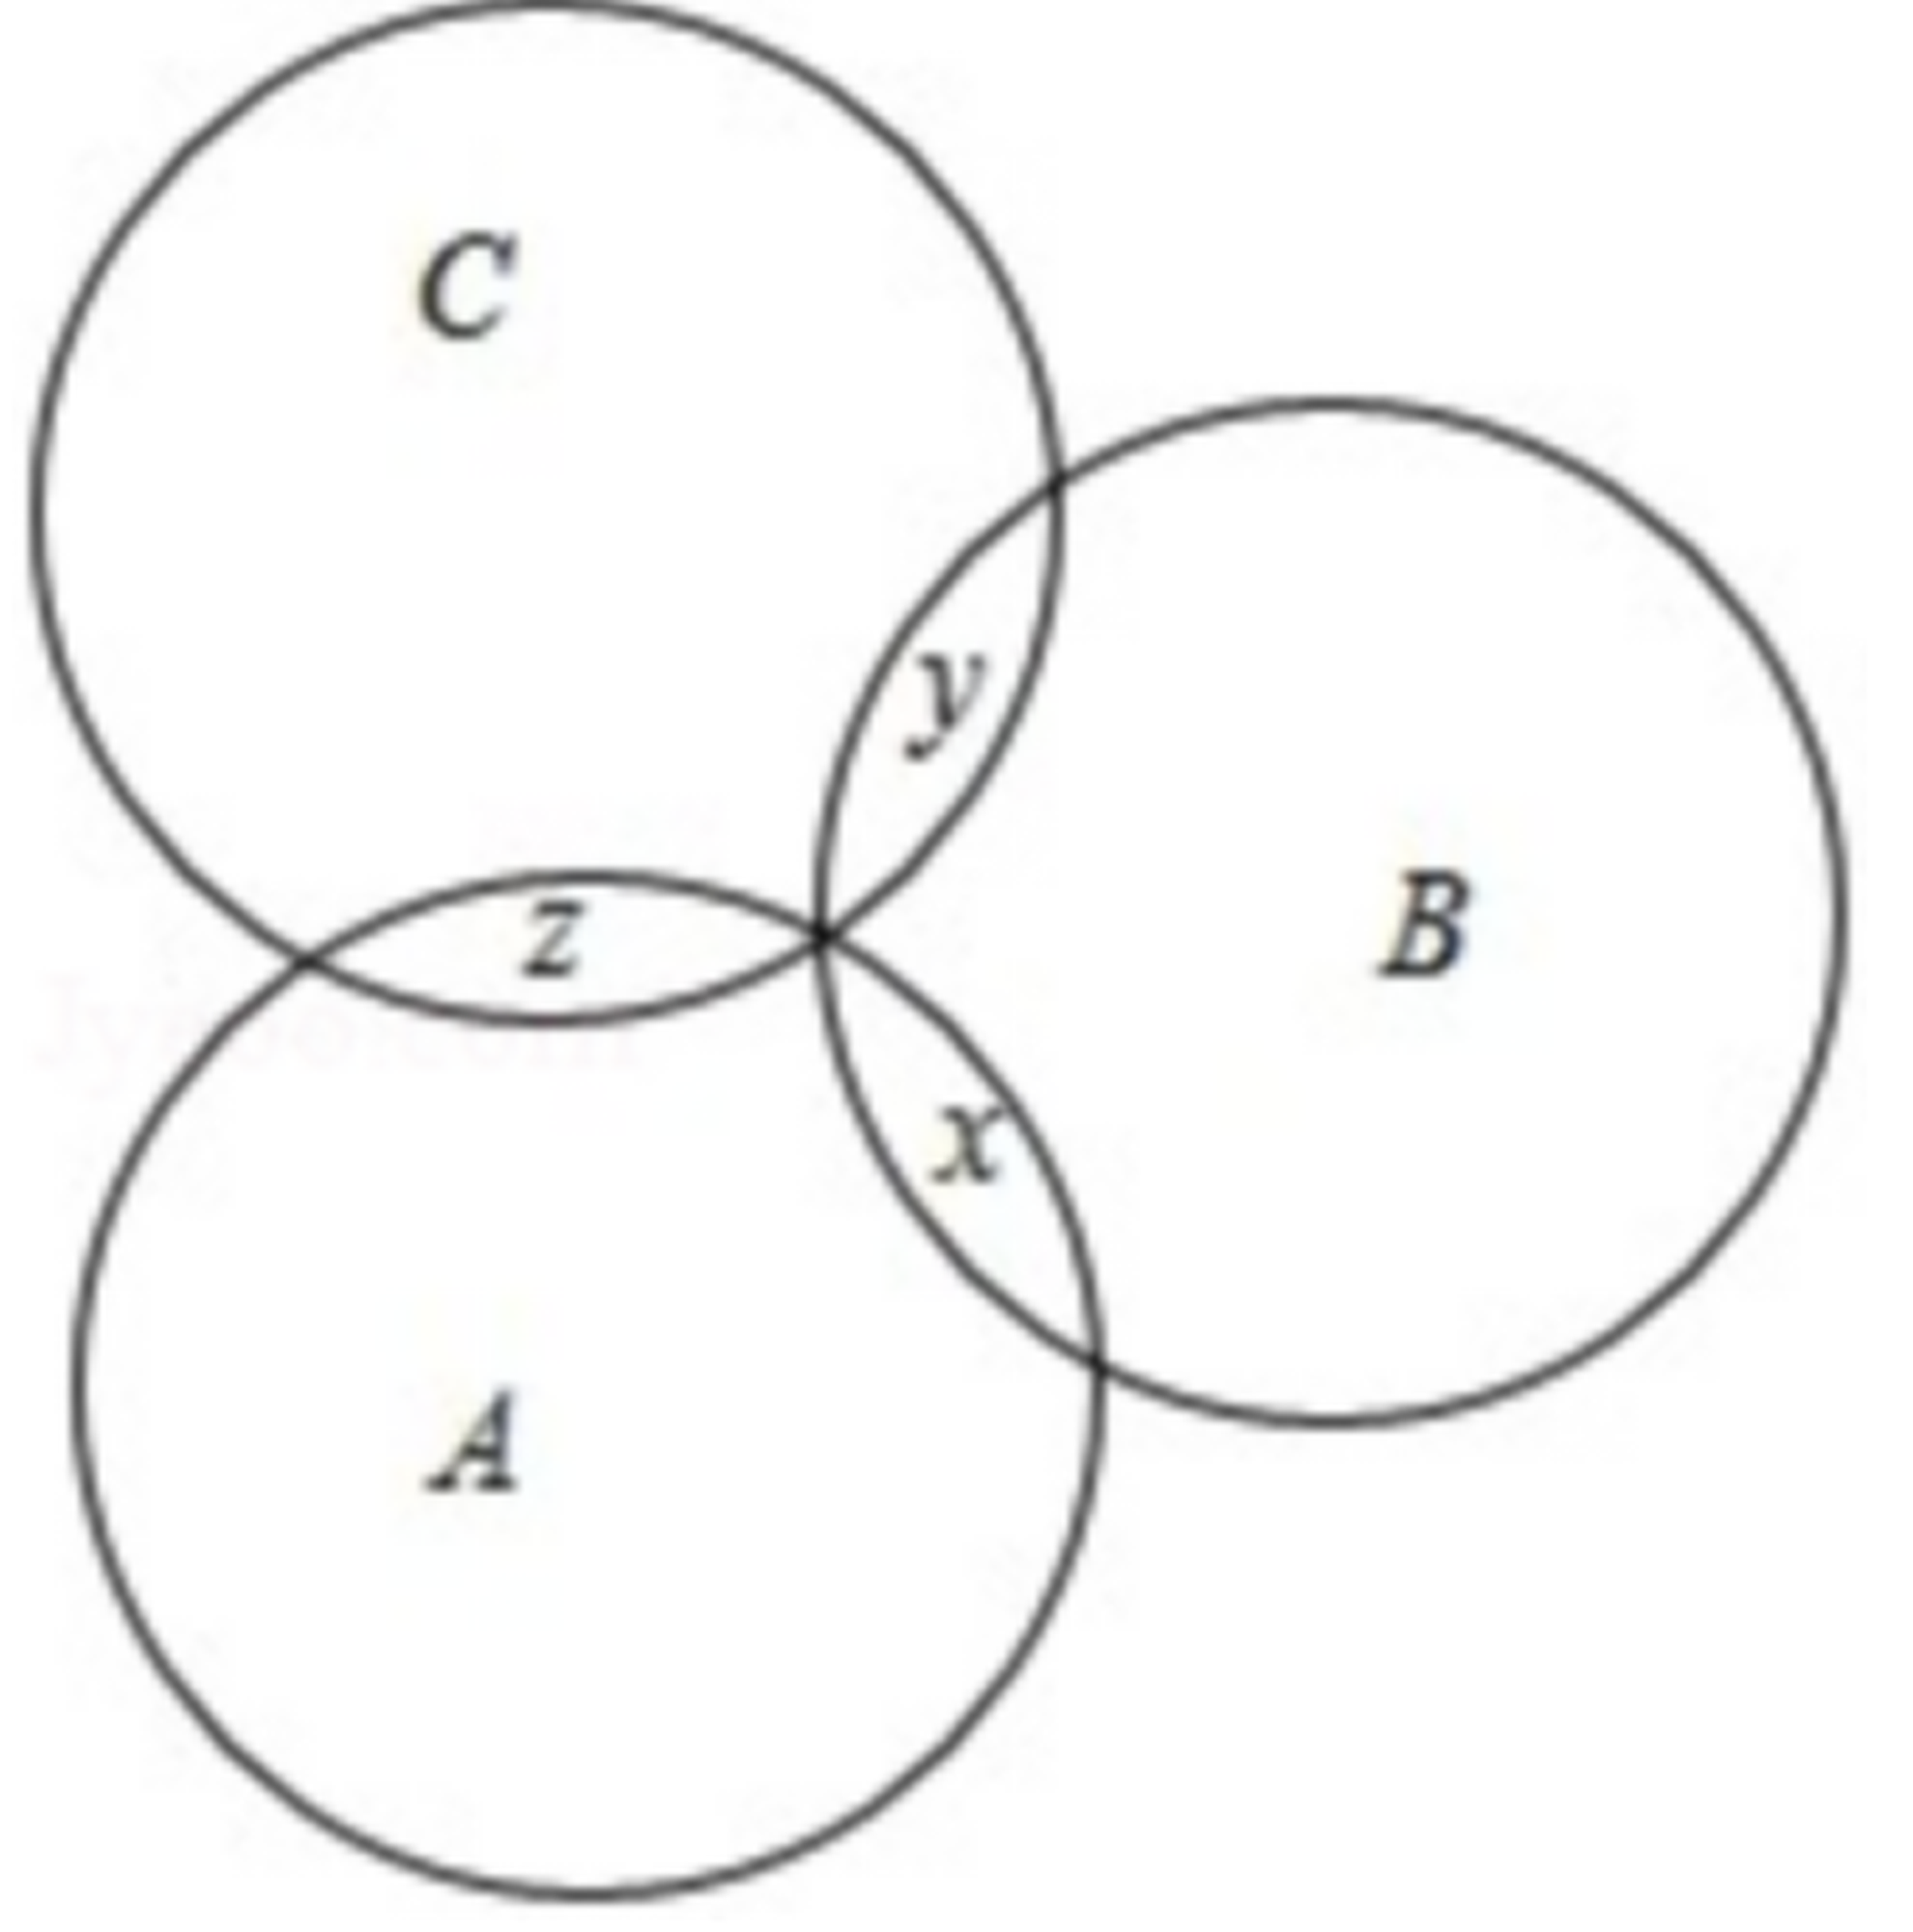
\includegraphics[width=0.30\textwidth]{figures/venn_ABC_x_y_z_h39.png}
\end{center}
\step{因为 $|A\cap B|=|B\cap C|=|C\cap A|=1$，且 $x$、$y$、$z\in\{1,2,3\}$，}
\step{所以集合 $A=\{x,z\}$，$B=\{x,y\}$，$C=\{z,y\}$，}
\step{若 $x=1$，$y=2$，$z=3$，则 $A=\{1,3\}$，$B=\{1,3\}$，$C=\{2,3\}$，}
\step{将 $1$，$2$，$3$ 进行全排列，有 $P_3^3=3\times2=6$ 个.}
\solend

\fi

\item 已知集合 $T=\{1,2,\cdots,2025\}$，对于 $T$ 的每一个非空子集的所有元素，计算它们乘积的倒数，
则所有这样倒数的和为 \blankline[4.4em].

\ans{$2025$}

\ifanswer
\solbegin
\step{集合 $T=\{1,2,\cdots,2025\}$ 的非空子集的个数为 $2^{2025}-1$，}
\step{这些子集中，每个元素的乘积分别为}
\step{$1,2,3,\cdots,2025,1\times2,1\times3,\cdots,1\times2025,\cdots,1\times2\times3\times\cdots\times2025$，}
\step{每项都可以看作是从 $1,2,3,\cdots,2025$ 中选择若干项的乘积，}
\step{$1+\dfrac12+\cdots+\dfrac{1}{2025}+\dfrac{1}{1\times2}+\dfrac{1}{1\times3}+\cdots+\dfrac{1}{2024\times2025}
+\cdots+\dfrac{1}{1\times2\times\cdots\times2025}$}
\step{$=(1+1)\left(1+\dfrac12\right)\cdots\left(1+\dfrac{1}{2025}\right)-1
=2\times\dfrac32\times\dfrac43\times\cdots\times\dfrac{2026}{2025}-1=2025$.}
\solend

\fi

% 第 24 题是压轴题，题干较长；试卷版在它之前量一次页高，尽量不与前文分家（照全稿成例）。
\ansneed{5cm}
% 注：原卷【解析】①③ 两步把 $f(x)$ 印作 $f[x[x]]$，显系笔误，照录未改，见文件头「笔误/存疑」⑦。
\item 若 $X$ 是一个集合，$T$ 是一个以 $X$ 的某些子集为元素的集合，且满足：①$X$ 属于 $T$，
$\varnothing$ 属于 $T$；②$T$ 中任意多个元素的并集属于 $T$；③$T$ 中任意多个元素的交集属于 $T$.
则称 $T$ 是集合 $X$ 上的一个拓扑. 已知函数 $f(x)=[x[x]]$，其中 $[x]$ 表示不大于 $x$ 的最大整数，
当 $x\in(0,n]$，$n\in\N^*$ 时，函数 $f(x)$ 值域为集合 $A_n$，则集合 $A_2$ 上的含有 $4$ 个元素的
拓扑 $T$ 的个数为 \blankline[4.4em].

\ans{$9$}

\ifanswer
\solbegin
\step{由题意，$n=2$，故 $0<x\leqslant2$，}
\step{①当 $0<x<1$ 时，则 $[x]=0$，所以 $f[x[x]]=0$，}
\step{②当 $x=1$ 时，$[x]=1$ 显然 $f(1)=1$，}
\step{③当 $1<x<2$ 时，$[x]=1$，所以 $f[x[x]]=[x]=1$，}
\step{④当 $x=2$ 时，$f(2)=4$，}
\step{所以 $A_2=\{0,1,4\}$，}
\step{因为 $T$ 中含有 $4$ 个元素，其中两个元素 $\varnothing$ 和 $A_2$，}
\step{$A_2=\{0,1,4\}$. 其它两个元素为 $A$、$B$，则
$\begin{cases}A\neq\varnothing\\ A\neq A_2\\ B\neq\varnothing\\ B\neq A_2\\ A\neq B\end{cases}$，}
\step{由对称性，不妨设 $1\leqslant|A|\leqslant|B|\leqslant2$，其中 $|A|$、$|B|$ 表示集合 $A$ 中元素的个数，}
\step{因为 $\begin{cases}A\cap B\in T\\ A\cup B\in T\end{cases}$，又 $|A|\leqslant|B|$，所以 $A\cap B=\varnothing$ 或 $A$，}
\step{若 $A\cap B=\varnothing$，则 $A\cup B$ 只能等于 $A_2$，}
\step{（若 $A\cup B=B$，则 $A\sub B$，则 $A\cap B=A=\varnothing$，矛盾）}
\step{则必有 $\begin{cases}|A|=1\\ |B|=2\end{cases}$，所以 $(A,B)$ 的个数 $\Leftrightarrow$ $A$ 的个数 $=3$ 种，}
\step{即 $\begin{cases}A=\{0\}\\ B=\{1,4\}\end{cases}$ 或 $\begin{cases}A=\{1\}\\ B=\{0,4\}\end{cases}$
或 $\begin{cases}A=\{4\}\\ B=\{0,1\}\end{cases}$；}
\step{若 $A\cap B=A\Leftrightarrow A\sub B$ 此时满足 $A\cup B=B$，}
\step{因为 $A\neq B$ 且 $1\leqslant|A|$ 且 $|B|\leqslant2$，所以 $\begin{cases}|A|=1\\ |B|=2\end{cases}$，}
\step{所以 $B$ 的选择共有 $C_3^2=3$ 种，则 $A$ 的个数有 $C_2^1$ 种，}
\step{所以 $(A,B)$ 的个数 $=2\times3=6$ 种.}
% 这六组「$A$／$B$」按原卷排作两行（前五个一行、第六个另起一行）；因五组并排时
% amsmath 的 cases 会为每组的第二列各留一枚 \quad，本行改排 \left\{\begin{matrix}…\end{matrix}\right.
% 以省下这枚 \quad（照 README「说明」记的高一07 成例），字形与 cases 相同。
\step{（这 $6$ 种是 $\left\{\begin{matrix}A=\{0\}\\ B=\{0,1\}\end{matrix}\right.$、
$\left\{\begin{matrix}A=\{1\}\\ B=\{0,1\}\end{matrix}\right.$、
$\left\{\begin{matrix}A=\{0\}\\ B=\{0,4\}\end{matrix}\right.$、
$\left\{\begin{matrix}A=\{4\}\\ B=\{0,4\}\end{matrix}\right.$、
$\left\{\begin{matrix}A=\{1\}\\ B=\{1,4\}\end{matrix}\right.$、}
\step{$\left\{\begin{matrix}A=\{4\}\\ B=\{1,4\}\end{matrix}\right.$）.}
\step{综上，$T$ 的个数为 $9$ 个.}
\solend

\fi

\end{enumerate}

\end{document}
"
% 紧凑版：xelatex "\def\iscompact{1}% 高一39_大同中学_周末作业4.1.tex
%   —— 高一上数学「2026-2027 年大同中学高一上周末作业 4.1」（试卷版/答案版）
% 试卷版：xelatex 高一39_大同中学_周末作业4.1.tex
% 答案版：xelatex "\def\isanswer{1}\input{高一39_大同中学_周末作业4.1.tex}"
% 紧凑版：xelatex "\def\iscompact{1}\input{高一39_大同中学_周末作业4.1.tex}"
%
% 原始材料是微信公众号图文（公众号「魔都数学加油站」连载「27学年高一 39」，署名「破晓」，
% 2026-09-26 21:29 发布，原文标题「27学年高一39——2026-2027年上海市大同中学高一上周末作业4.1」，
% 原文链接 https://mp.weixin.qq.com/s/HR2hIayXUXNi4zTs3PioiQ ），正文为 11 张 PNG 页。**同一篇里各页分辨率不一致**（2560×3620 与 4762×6735 两档混排：第 1、3、8、10 页为
% 2560×3620，第 2、4、5、6、7、9、11 页为 4762×6735）。原文本身就是一份**讲评版**——除第 15 题
% 外各题题下直接印【解析】（无单独的【答案】行），第 15 题的答案「D」直接印在题干末尾的括号内。
% 试题文字、答案与解析均照原卷录入，未改内容。卷面的粉色斜水印「魔都数学加油站」属水印，未录入。
%
% 卷首标题：原卷页首印作「2026-2027 年大同中学高一上周末作业 4.1」（**卷面标题行即带校名**，
% 年份区间按全稿惯例排 en dash，前缀照原卷保留「年」）。
%
% 篇幅与题号：卷面自「一、填空题」的**第 3 题**起编，终于「附加题」的**第 24 题**，共 22 题
% （填空 3—12、选择 13—16、解答 17—20、附加题 21—24）。第 1、2 题未在该文中发布——这是该
% 公众号连载讲评版的通例（高一02—高一09 等均自第 3 题起编，README「说明」已记），**不是截断**，
% 故本稿题号亦自 3 起。它与 高一40（大同中学 周末作业4.2）同属「周末作业 4」系列但**各自独立起编**
% （4.2 自第 3 题起、终于第 19 题），不是同一份试卷的两半。
%
% 与原卷的排版差异（均已在 README「说明」中交代）：
%   ① 原文自**第 3 题**起（第 1、2 题未在该文中发布），故本稿题号亦自 3 起，填空题以
%      \setcounter{enumi}{2} 起编；选择、解答、附加题三节各按上一节末号另设 \setcounter
%      （选择题 \setcounter{enumi}{12}、解答题 \setcounter{enumi}{16}、附加题 \setcounter{enumi}{20}）；
%   ② 原卷本就印有「一、填空题」「二、选择题」「三、解答题」三节标题，末节印作「附加题」
%      （**不带「四、」**，且题号 21—24 续前编、不另起），本稿照原卷分节，只把标题改排成全稿
%      统一的「大节标题」样式；
%   ③ 原卷是「讲评版」：除第 15 题外，各题题下均印【解析】（**全卷无一条独立的【答案】行**）；
%      第 15 题无解析，答案「D」直接印在题干末尾的括号内。本稿统一改为试卷版隐去、答案版以
%      \ans{}／\ifanswer 块给出，两版彻底分离；原卷写在【解析】末句的结果，本稿照 高一38
%      （同校同系列、同为讲评版）的成例另提为 \ans{}；
%   ④ 数集记号原卷两套并用：实数集作斜体的 $R$（第 7、11、14、17、18、19 题），整数集作斜体
%      $Z$（第 10 题），自然数集作斜体 $N$ 及 $N^*$（第 16、20、21、24 题），本稿按全稿惯例
%      统一写作 $\R$、$\Z$、$\N$、$\N^*$；
%   ⑤ 补集符号原卷两套并用：第 7 题作前缀式的 $C_U$（且题干称全集为 $I$，见「笔误/存疑」①），
%      第 14、15、18 题作上横线（$\overline{H}$、$\overline{A}$、$\overline{B}$），本稿照录、不归一
%      （前缀式写作 $\complement_U$，与 高一c／高一10 的成例一致）；
%   ⑥ 包含符号原卷两套并用：第 3 题作**无下划线**的 $\subset$，第 15、18、20、24 题作**带下划线**
%      的 $\sub$，本稿照录、不归一；
%   ⑦ 原卷填空的横线约两个字宽，本稿按全稿惯例统一排 \blankline[4.4em]；
%   ⑧ 第 7、11、22 题各有插图，取原卷截图、4× LANCZOS 放大（figures/venn_N_cap_CI_M_h39.png、
%      figures/plane_grid_4squares_h39.png、figures/venn_ABC_x_y_z_h39.png）；第 7 题的 Venn 属
%      **题干**（试卷版、答案版都出），第 11、22 题的图在【解析】内（仅答案版出）。第 7 题图
%      左下、第 11 题图的上／左／右边缘带进极淡的原卷粉色水印残影——照全稿「插图直接取自
%      原卷截图、不用 TikZ 重绘、不修图」的体例保留（再裁会切到坐标轴与 $x$、$y$、$O$ 标注）；
%   ⑨ 原卷并列的字母、数字（「$x_1,x_2$」「$a,b$」「$1,2,3,\cdots,11$」）多作半角逗号或不加标点，
%      本稿按全稿惯例改排顿号（$x_1$、$x_2$）或把数列并入行内公式；半角括号、逗号一律排全角，
%      数学式内部的标点照原样；
%   ⑩ 原卷未印副标题，本稿按**本卷实际内容**补出副标题「集合与常用逻辑用语」（依据见下条）。
%
% 副标题（\examtitlest 第二个参数）：本卷卷面未印副标题，由本稿补出，取值按 2026-09-26 起的
%   新口径「只用本卷实际内容的模块名」定为「集合与常用逻辑用语」。依据：全卷 22 题（第 3—24 题）中，
%   第 3、5、7、8、10、11、14、15、16、17、18、19、20、21、22、23、24 题共 17 题是集合的运算与
%   关系、子集／真子集、补集、集合新定义（「全食／偏食」、最小相交、拓扑、特征数）与集合计数，
%   以及命题与常用逻辑用语（第 3 题充要条件、第 5 题存在量词命题、第 17 题命题真假）；其余两题
%   第 4、6 考一元二次方程的根（韦达定理）与方程恒等，第 9、12、13 题是不等式（一元二次不等式组
%   的整数解、一元二次不等式解集、不等式的性质）——不等式合计 3/22，**不足全卷三分之一**，
%   故不并标「不等式」。
%
% 原卷笔误/存疑（均照抄原卷、未改，见源码中该处上方注释）：
%   ① 第 7 题题干称「全集 $I=R$」，而【解析】两处把补集写作 $C_U M$（下标作 $U$），前后记号不一；
%      本稿照录，未改；
%   ② 第 4 题【解析】两处把判别式印作 $\triangle=[2(m-1)^2-16m^2]$（方括号内首项漏了平方，
%      正确应作 $[2(m-1)]^2-16m^2$）；按其所判「$m=\frac12$ 时 $<0$、$m=-\frac12$ 时 $>0$」反推，
%      $[2(m-1)]^2-16m^2$ 在 $m=\frac12$ 时为 $-3<0$、在 $m=-\frac12$ 时为 $5>0$，与结论一致；
%      本稿照录；
%   ③ 第 9 题【解析】把方程组第二式印作 $1-2<-k\leqslant3$，按其结论 $-3\leqslant k<2$ 反推，
%      疑当作 $-2<-k\leqslant3$（原卷多一个「$1$」）；本稿照录；
%   ④ 第 17 题【解析】首句「由数 $y=-x^2+ax-1=-x+3$」中的「由数」显系「由」或「由函数」之误；
%      且末段「若 $p$ 真 $q$ 假…得 $a\in R$」「若 $p$ 假 $q$ 真…此时 $a$ 无解」与结论「$a$ 的取值范围
%      是 $R$」自相矛盾（按 $p:a\leqslant-5$、$q:a>-6$，$p$ 真 $q$ 假应为 $a\leqslant-6$，$p$ 假 $q$ 真
%      应为 $a>-5$，合起来是 $a\leqslant-6$ 或 $a>-5$，并非 $R$）；本稿一律照录，未按正确解法改写；
%   ⑤ 第 18 题【解析】(2) 把 $B=\{x\mid x^2+a\leqslant0\}$（$a<0$）印作右端开的
%      $\{x\mid-\sqrt{-a}\leqslant x<\sqrt{-a}\}$（应为闭的「$\leqslant$」）；按其所判
%      $\sqrt{-a}<\frac12$ 反推，不影响结论；本稿照录；
%   ⑥ 第 22 题【解析】在 $x=1$、$y=2$、$z=3$ 时把 $B=\{x,y\}$ 印作 $\{1,3\}$（应为 $\{1,2\}$），
%      与本行前面「$B=\{x,y\}$」不合；本稿照录；
%   ⑦ 第 24 题【解析】①③ 两步把 $f(x)$ 印作 $f[x[x]]$，显系笔误；本稿照录。
%   ⑧ 第 8 题【解析】「即方程 $x^2+ax+b=x$，$x^2+(a-1)x+b=0$ **由**两个相等的实数根为 $4$」——
%      「由」当为「有」（「设…是…有」的杂糅）；本稿照录；
%   ⑨ 第 10 题：题设 $a\oplus b=b(a^2+b^2+1)$，而集合定义里含 $\dfrac{a\oplus b}{2b}$；$-2<a<b<2$、
%      $a$、$b\in\Z$ 时 $(a,b)=(-1,0)$ 也合条件、却使分母 $2b=0$，原卷解析仍代入该组并约去
%      $b$ 得 $x=1$（答案集恰好不变）；本稿照录；
%   ⑩ 第 15 题选项列里 ② 与 ③ 之间**漏排分隔号**（原卷作「② $\overline{A}\cap B=\varnothing$③
%      $\overline{A}\sub\overline{B}$；」——①、③ 后都有「；」，② 后没有）；本稿照录；
%   ⑪ 第 20(2) 把 $\{1,2,\cdots,20\}$ 分成的 11 个集合里，$\{8,11\}$ 与 $\{9,12\}$ 之间误用
%      **句号**「.」（同行其余处皆逗号）；本稿照录；
%   ⑫ 第 20(3)① 推理不严：原卷写「选 5 则不选 1、9；选 6 则不选 2、10；选 7 则不选 3、11；
%      则只剩 4、8」——但 4 与 8 相差 $4$、不能同选，该情形实际最多只能取 $4$ 个；末句结论
%      「不超过 $5$ 个」仍成立；本稿照录；
%   ⑬ 第 16 题【解析】两种下标并存：「所以在 $A_i$ 的特征数构成中」原卷作斜体 $A_i$，而
%      「要使 $X_1+X_2+X_3$ 最大（小），则（应）在集合 $A_1$ 中首先放置…」两处原卷作
%      **数字 $1$**（与同句 $X_1$ 的角标同形）；本稿照录、未归一。
%
% 图取原卷截图（依次见各处的 \includegraphics 前的注释），4× LANCZOS 放大。
\documentclass[a4paper,11pt]{article}
\usepackage{common}

\begin{document}

\examtitlest[3]{2026--2027 年大同中学高一上周末作业 4.1}{集合与常用逻辑用语}

\bigsec{一、填空题}

\begin{enumerate}
\setcounter{enumi}{2}

\item “$x\geqslant a$”是“$0<x<2$”的必要非充分条件，则实数 $a$ 的取值范围是 \blankline[4.4em].

\ans{$(-\infty,0]$}

\ifanswer
\solbegin
\step{因为 $x\geqslant a$ 是 $0<x<2$ 的必要非充分条件，所以 $(0,2)\subset[a,+\infty)$，所以 $a\leqslant0$，}
\step{则实数 $a$ 的取值范围是 $(-\infty,0]$.}
\solend

\fi

% 注：原卷$[2(m-1)^2-16m^2]$ 首项漏了平方（应为 $[2(m-1)]^2-16m^2$），照录未改，见文件头「笔误/存疑」②。
\item 若关于 $x$ 的方程 $x^2+2(m-1)x+4m^2=0$ 有两个实数根，且这两根互为倒数，则 $m=$ \blankline[4.4em].

\ans{$-\dfrac12$}

\ifanswer
\solbegin
\step{设 $x_1$、$x_2$ 是方程 $x^2+2(m-1)x+4m^2=0$ 有两个实数根，}
\step{则 $x_1x_2=4m^2=1$，解得 $m=\dfrac12$ 或 $m=-\dfrac12$，}
\step{又当 $m=\dfrac12$ 时，$\triangle=[2(m-1)^2-16m^2]<0$，舍去，}
\step{当 $m=-\dfrac12$ 时，$\triangle=[2(m-1)^2-16m^2]>0$，故 $m=-\dfrac12$.}
\solend

\fi

\item 已知命题：“存在 $x\in[1,2]$，使 $x^2+2x+a\geqslant0$”为真命题，则 $a$ 的取值范围是 \blankline[4.4em].

\ans{$a\geqslant-8$}

\ifanswer
\solbegin
\step{若存在 $x\in[1,2]$，使 $x^2+2x+a\geqslant0$，}
\step{则等价为存在 $x\in[1,2]$，使 $x^2+2x\geqslant-a$，}
\step{当存在 $x\in[1,2]$ 时，设 $y=x^2+2x=(x+1)^2-1$，则 $3\leqslant y\leqslant8$，}
\step{所以要使 $x^2+2x\geqslant-a$，则 $8\geqslant-a$，即 $a\geqslant-8$.}
\solend

\fi

\item 已知方程 $a(3x+2)+b(2x-3)=8x+3$ 有无穷多个解，则 $a:b=$ \blankline[4.4em].

\ans{$30:7$}

\ifanswer
\solbegin
\step{$a(3x+2)+b(2x-3)=(3a+2b)x+2a-3b=8x+3$ 有无穷多个解，}
\step{所以 $\begin{cases}3a+2b=8\\ 2a-3b=3\end{cases}$，解得 $a=\dfrac{30}{13}$，$b=\dfrac{7}{13}$，所以 $a:b=30:7$.}
\solend

\fi

% 注：原卷题干称「全集 $I=R$」，而【解析】两处把补集写作 $C_U M$（下标作 $U$），前后记号不一；
%     照录未改，见文件头「笔误/存疑」①。
\item 已知集合 $M=\{x\mid y=\sqrt{3-x^2}\}$，$N=\{x\mid-3\leqslant x\leqslant1\}$，全集 $I=\R$，
则图中阴影部分表示的集合为 \blankline[4.4em].

% 图取原卷截图（01.png，2560×3620）右栏，4× LANCZOS 放大。
\begin{center}
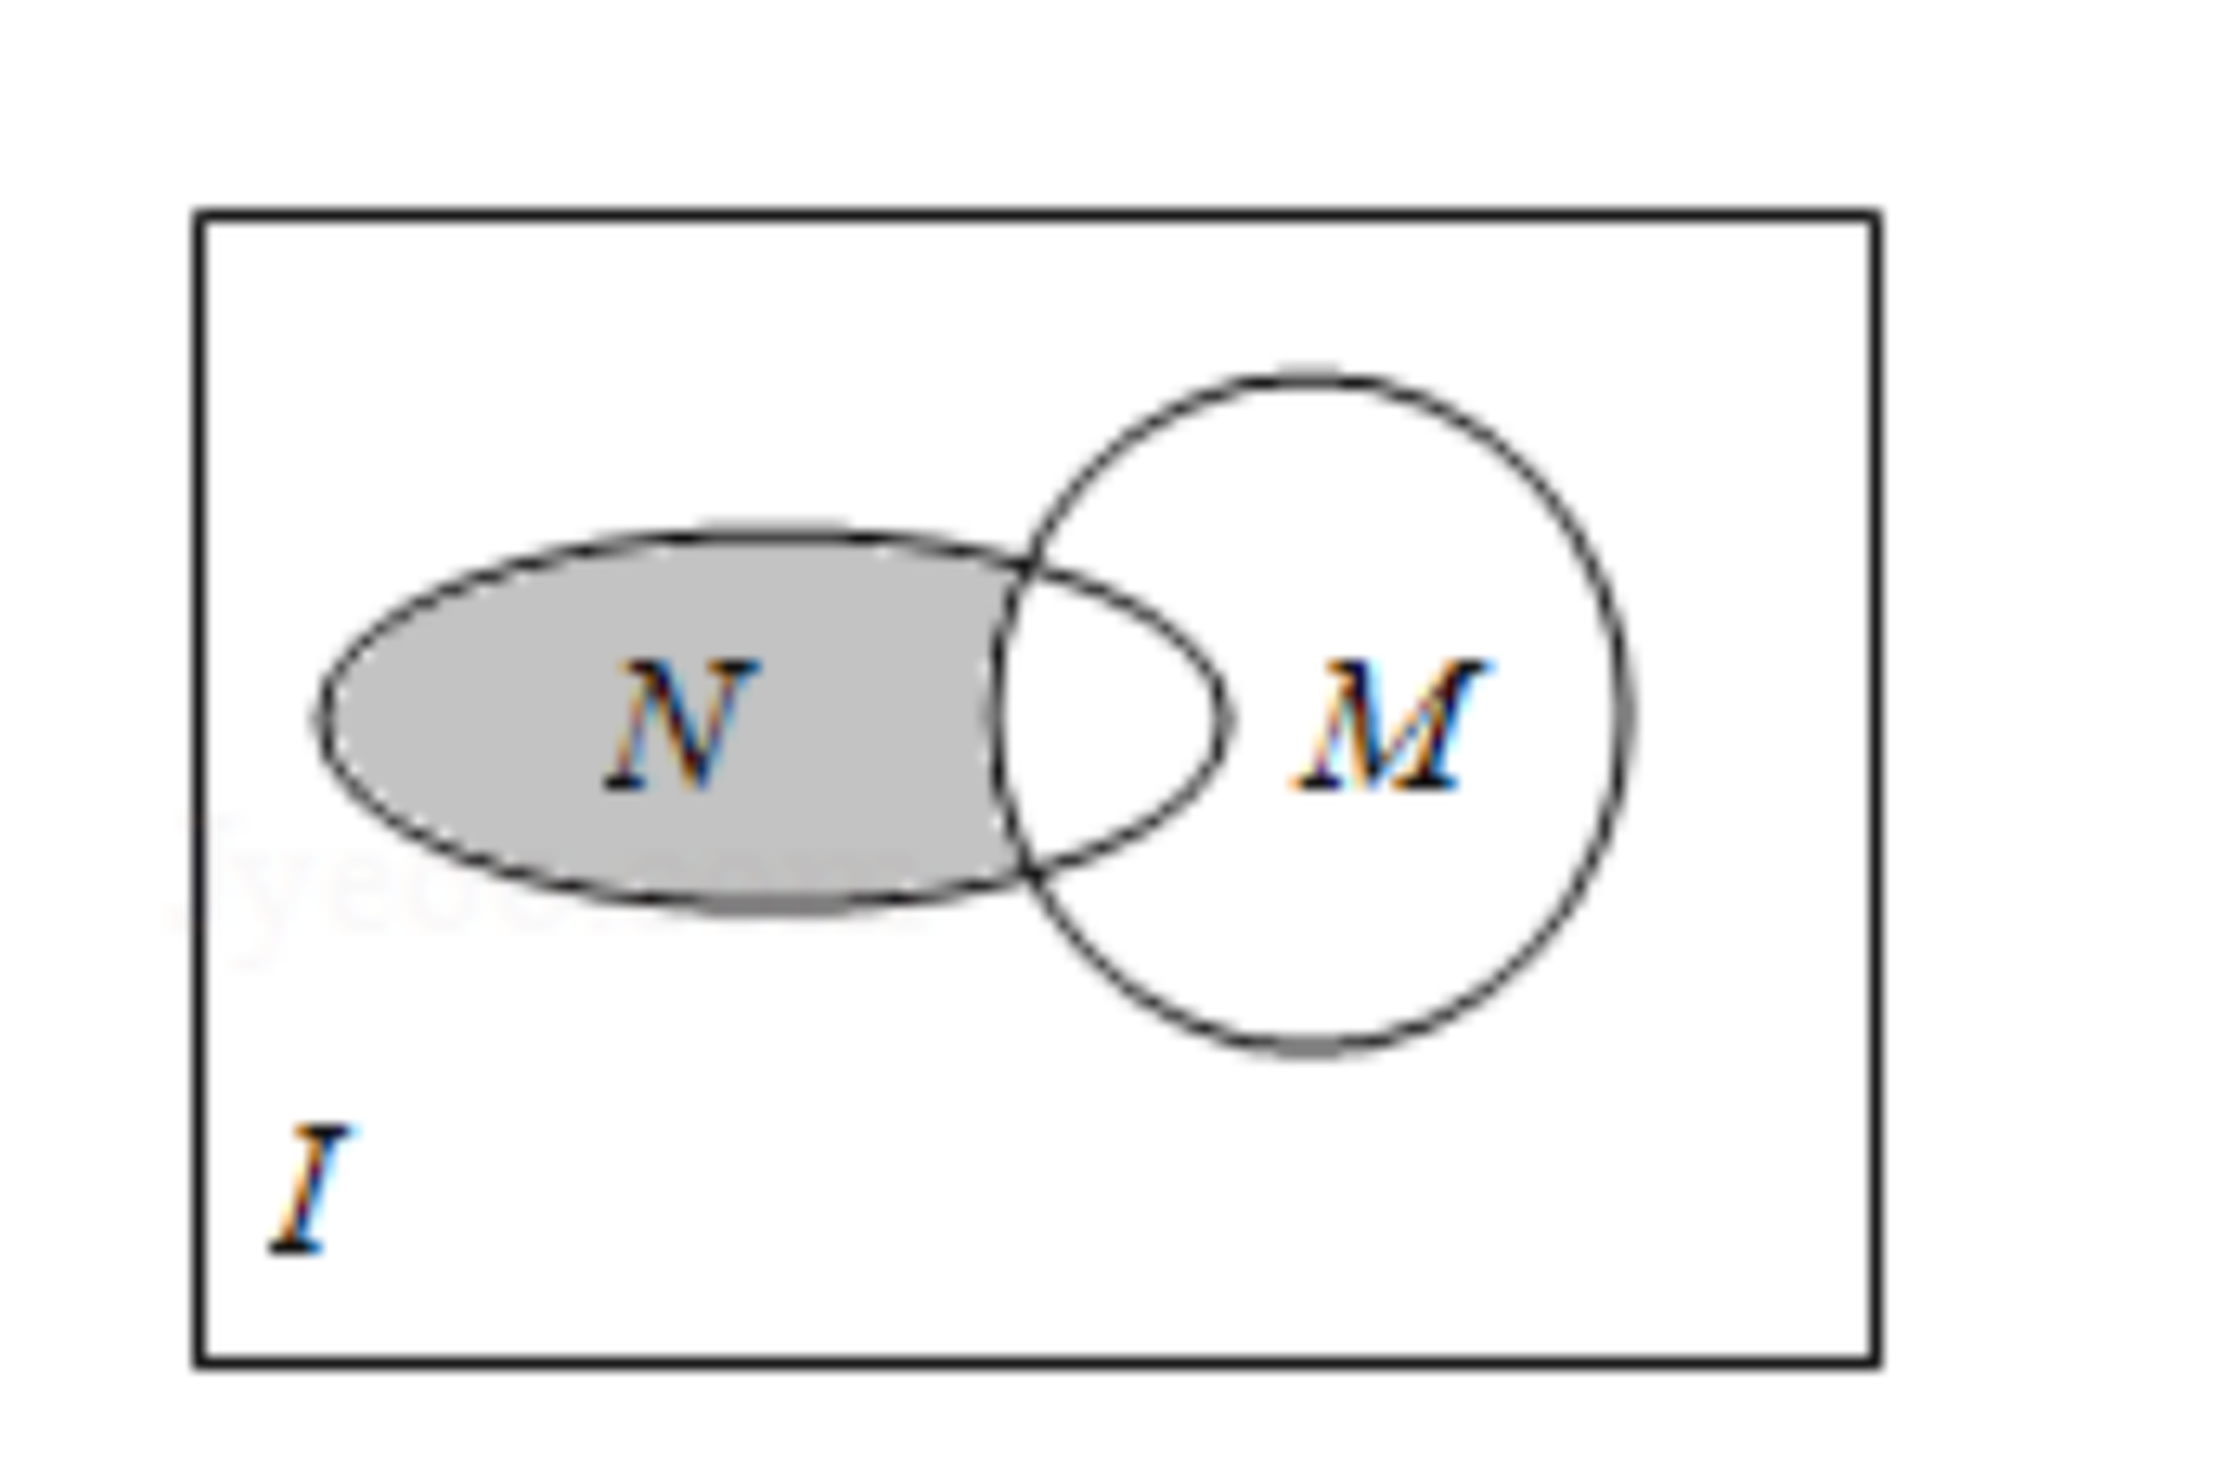
\includegraphics[width=0.30\textwidth]{figures/venn_N_cap_CI_M_h39.png}
\end{center}

\ans{$[-3,-\sqrt3)$}

\ifanswer
\solbegin
\step{阴影部分用集合表示为 $N\cap(\complement_UM)$.}
\step{则 $M=\{x\mid y=\sqrt{3-x^2}\}=\{x\mid3-x^2\geqslant0\}=\{x\mid-\sqrt3\leqslant x\leqslant\sqrt3\}$，}
\step{则 $\complement_UM=\{x\mid x>\sqrt3\text{ 或 }x<-\sqrt3\}$，$N=\{x\mid|x+1|\leqslant2\}=\{x\mid-3\leqslant x\leqslant1\}$，}
\step{则 $N\cap(\complement_UM)=\{x\mid-3\leqslant x<-\sqrt3\}$.}
\solend

\fi

\item 已知 $f(x)=x^2+ax+b$，集合 $\{x\mid f(x)=x\}=\{4\}$，将集合 $M=\{x\mid f(x)=4\}$ 用列举法表示 \blankline[4.4em].

\ans{$\{3,4\}$}

\ifanswer
\solbegin
\step{已知 $f(x)=x^2+ax+b$，集合 $\{x\mid f(x)=x\}=\{4\}$，}
% 注：原卷本行作「…$x^2+(a-1)x+b=0$ **由**两个相等的实数根为 $4$」——「由」当为「有」
%     （「设…是…有」的杂糅）；本稿照录未改，见文件头「原卷笔误/存疑」⑧。
\step{即方程 $x^2+ax+b=x$，$x^2+(a-1)x+b=0$ 由两个相等的实数根为 $4$，}
\step{所以 $\triangle=(a-1)^2-4b=0$，即 $x^2+(a-1)x+b=(x-4)^2$，所以 $b=16$，$a=-7$，}
\step{所以 $f(x)=x^2+ax+b=x^2-7x+16$，所以集合 $M=\{x\mid f(x)=4\}$，}
\step{即 $x^2-7x+16=4$，$x^2-7x+12=0$，故 $M=\{x\mid f(x)=4\}=\{3,4\}$.}
\solend

\fi

% 注：原卷方程组第二式印作 $1-2<-k\leqslant3$，按其结论 $-3\leqslant k<2$ 反推疑当作 $-2<-k\leqslant3$，
%     照录未改，见文件头「笔误/存疑」③。
\item 关于 $x$ 的不等式组 $\begin{cases}x^2-x-2>0\\ 2x^2+(2k+5)x+5k<0\end{cases}$ 的整数解的集合为 $\{-2\}$，
则实数 $k$ 的取值范围 \blankline[4.4em].

\ans{$-3\leqslant k<2$}

\ifanswer
\solbegin
\step{原不等式组即 $\begin{cases}(x-2)(x+1)>0\\ (x+k)(2x+5)<0\end{cases}$，整数解的集合为 $A$，若 $A=\{-2\}$，}
\step{则 $(-2+k)(2\times(-2)+5)<0$，所以 $k<2$，且有 $\begin{cases}-k>-\dfrac52\\ 1-2<-k\leqslant3\end{cases}$，}
\step{解得 $-3\leqslant k<2$.}
\solend

\fi

\item 规定 $\oplus$ 与 $\otimes$ 是两个运算符号，其运算法则如下，对任意实数 $a$、$b$ 有：$a\otimes b=ab$，
$a\oplus b=b(a^2+b^2+1)$. 若 $-2<a<b<2$ 且 $a$、$b\in\Z$，
$A=\left\{x\mid x=2(a\otimes b)+\dfrac{a\oplus b}{2b}\right\}$，则用列举法表示集合 $A=$ \blankline[4.4em].

\ans{$\left\{1,-\dfrac12\right\}$}

\ifanswer
\solbegin
\step{$A=\left\{x\mid x=2(a\otimes b)+\dfrac{a\oplus b}{2b}\right\}
=\left\{x\mid x=2ab+\dfrac{b(a^2+b^2+1)}{2b}\right\}$}
\step{$=\left\{x\mid x=2ab+\dfrac12a^2+\dfrac12b^2+\dfrac12\right\}
=\left\{x\mid x=\dfrac12(a+b)^2+ab+\dfrac12\right\}$，}
% 注：题设含 $\dfrac{a\oplus b}{2b}$，而 $-2<a<b<2$、$a$、$b\in\Z$ 时 $(a,b)=(-1,0)$ 也合条件、
%     却使分母 $2b=0$；原卷解析仍代入该组并约去 $b$ 得 $x=1$（答案集恰好不变）。本稿照录，
%     见文件头「原卷笔误/存疑」⑨。
\step{当 $a=-1$，$b=0$ 时，$x=1$；当 $a=-1$，$b=1$ 时，$x=-\dfrac12$；}
\step{当 $a=0$，$b=1$ 时，$x=1$；所以 $A=\left\{1,-\dfrac12\right\}$.}
\solend

\fi

\item 高斯是德国著名的数学家，近代数学奠基者之一，享有“数学王子”的称号，为了纪念数学家高斯，
我们把取整函数 $y=[x]$，$x\in\R$ 称为高斯函数，其中 $[x]$ 表示不超过 $x$ 的最大整数，
如 $[1.1]=1$，$[-1.1]=-2$. 则点集 $P=\{(x,y)\mid[x]^2+[y]^2=1\}$
所表示的平面区域的面积是 \blankline[4.4em].

\ans{$4$}

\ifanswer
\solbegin
\step{$[x]^2+[y]^2=1$ 由 $\begin{cases}[x]=0\\ [y]=-1\end{cases}$ 或 $\begin{cases}[x]=0\\ [y]=1\end{cases}$
或 $\begin{cases}[x]=-1\\ [y]=0\end{cases}$ 或 $\begin{cases}[x]=1\\ [y]=0\end{cases}$ 四个平面区域组成，}
\step{即 $\begin{cases}0\leqslant x<1\\ -1\leqslant y<0\end{cases}$ 或 $\begin{cases}0\leqslant x<1\\ 1\leqslant y<2\end{cases}$
或 $\begin{cases}-1\leqslant x<0\\ 0\leqslant y<1\end{cases}$ 或 $\begin{cases}1\leqslant x<2\\ 0\leqslant y<1\end{cases}$，}
\step{作出平面区域如图所示，平面区域由四个边长为 $1$ 的正方形组成，}
% 图在【解析】内（仅答案版出），取原卷截图（03.png，2560×3620）中部，4× LANCZOS 放大。
\begin{center}
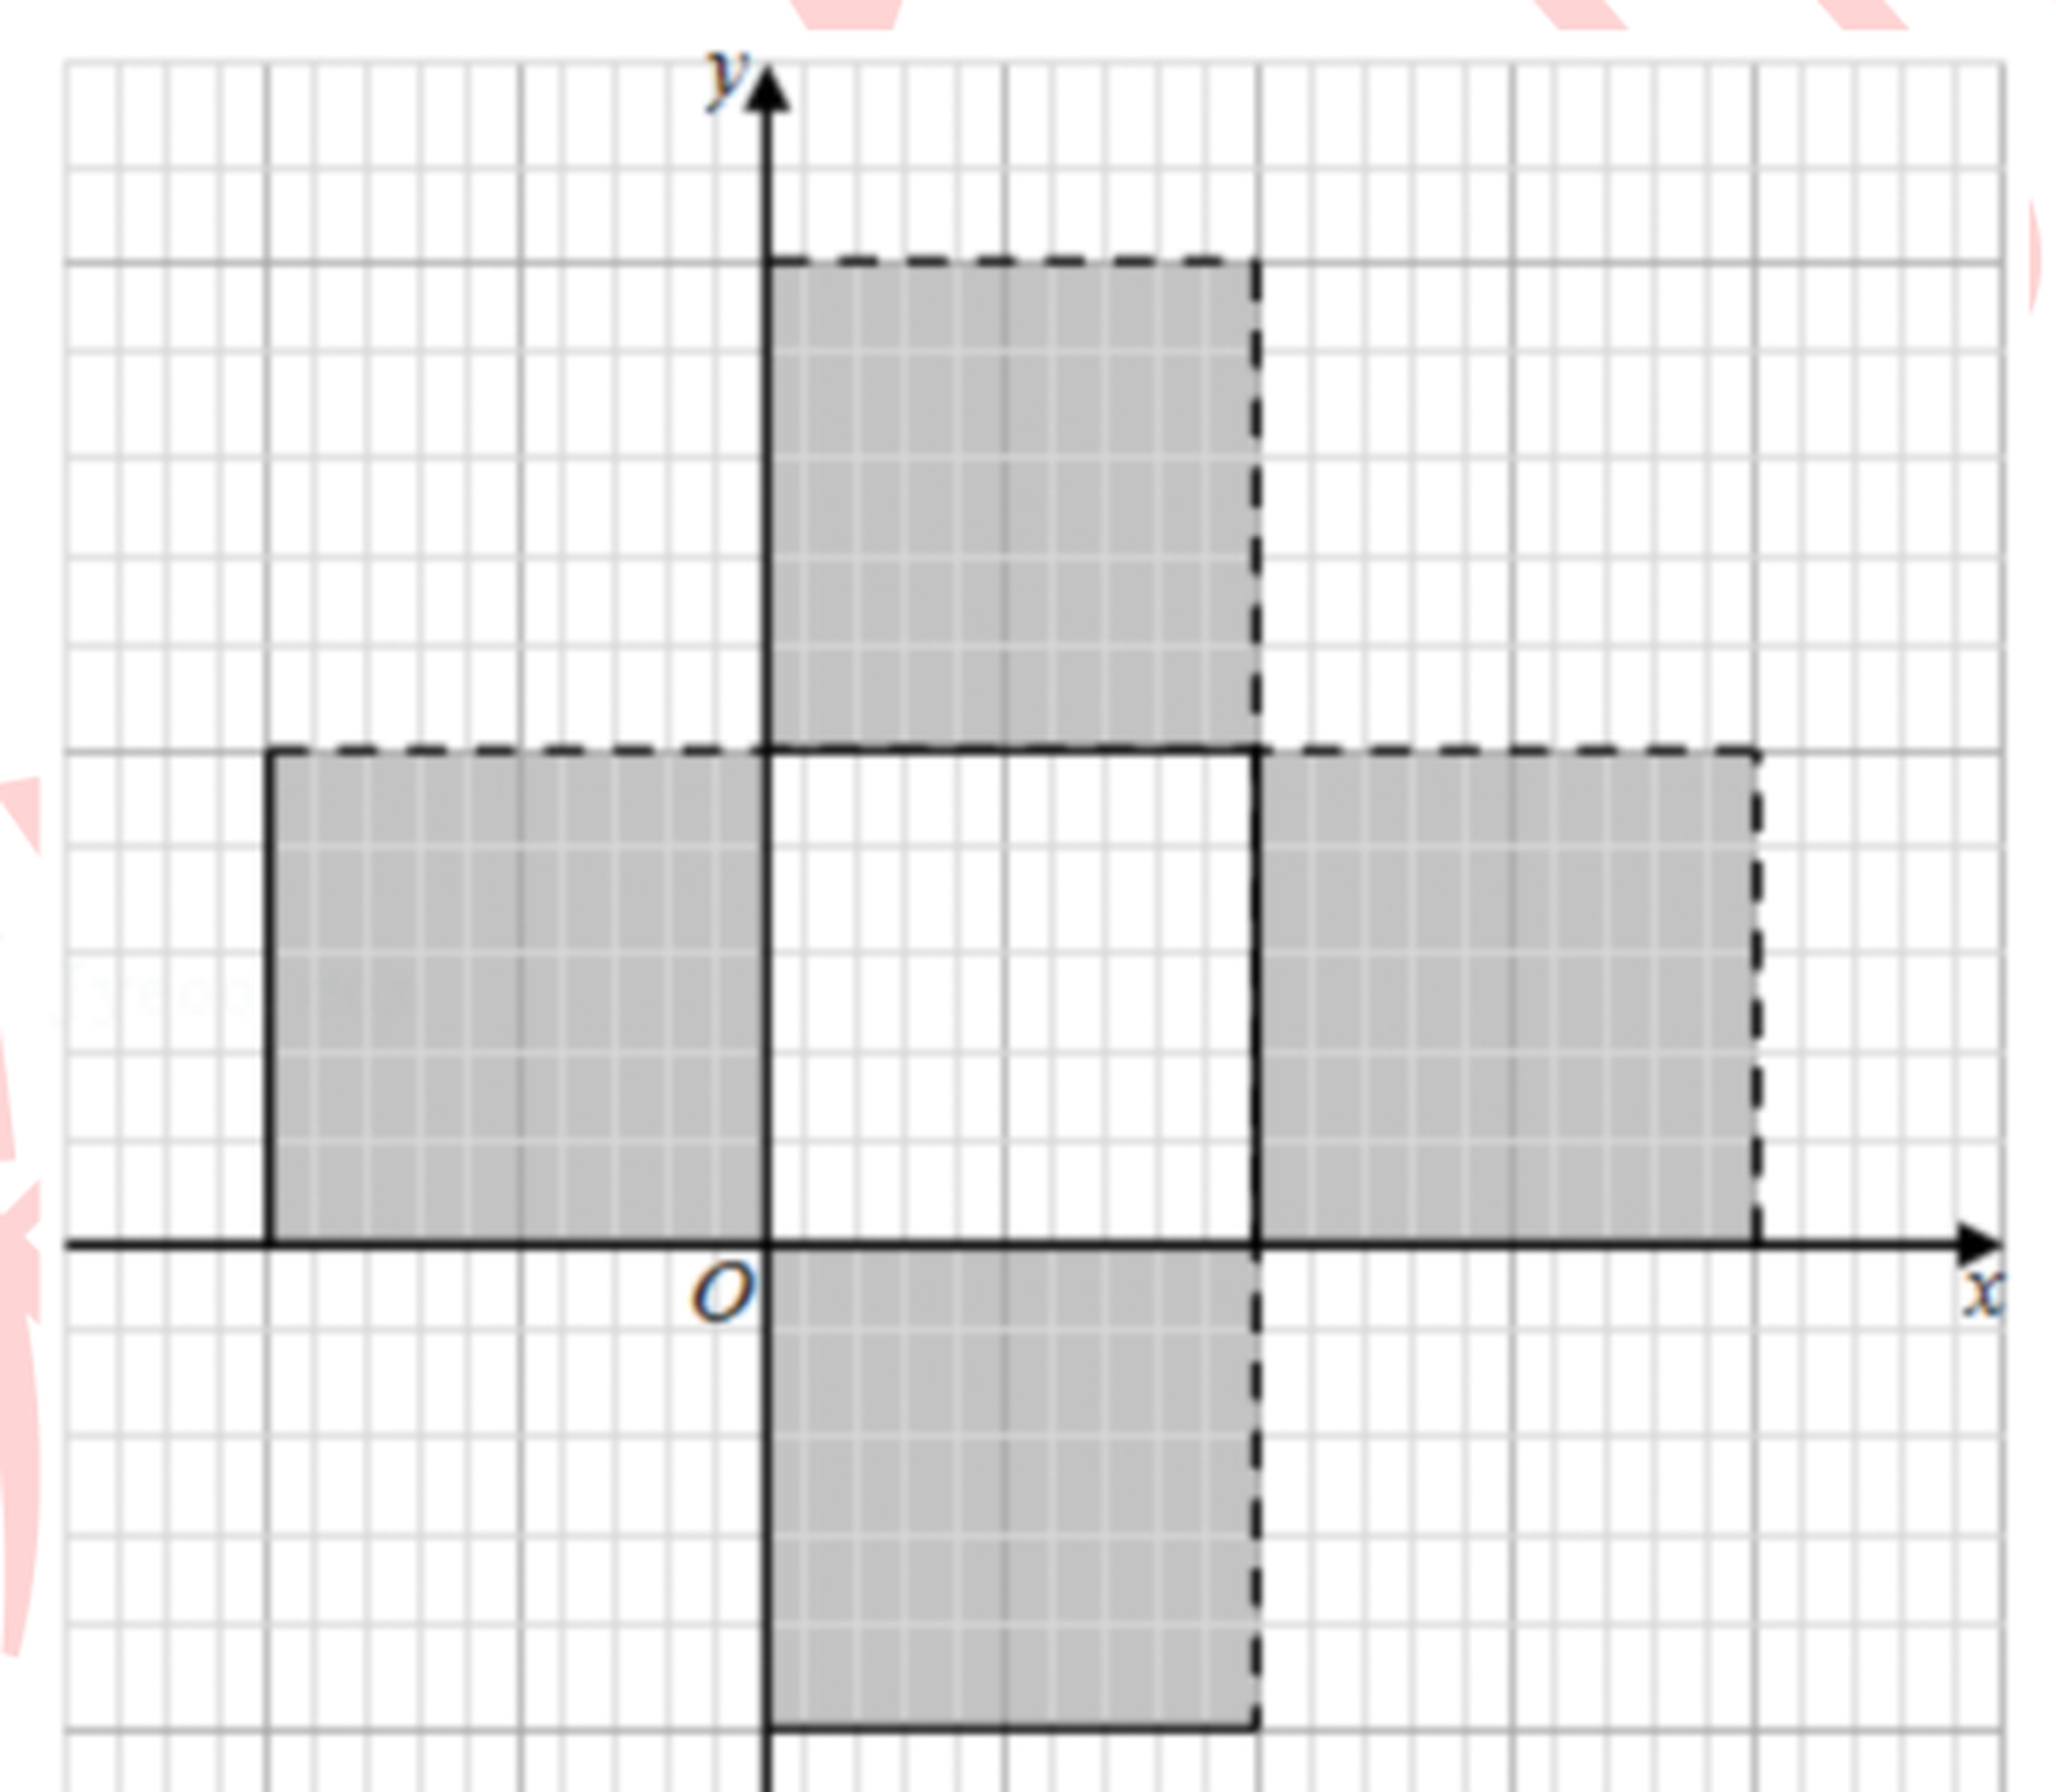
\includegraphics[width=0.38\textwidth]{figures/plane_grid_4squares_h39.png}
\end{center}
\step{总面积为 $1\times4=4$.}
\solend

\fi

\item 关于 $x$ 的不等式 $ax^2+bx+c>0$ 的解集为 $\{x\mid x<\beta\text{ 或 }x>\gamma\}(0<\beta<\gamma)$，
则不等式 $a(x^2+1)+b(x-1)+c>2ax$ 的解集为 \blankline[4.4em].

\ans{$(-\infty,\beta+1)\cup(\gamma+1,+\infty)$}

\ifanswer
\solbegin
\step{由题意得 $\beta$、$\gamma$ 为方程 $ax^2+bx+c=0$ 的两根且 $a>0$，}
\step{则 $\beta+\gamma=-\dfrac ba$，$\beta\gamma=\dfrac ca$，故 $b=-a(\beta+\gamma)$，$c=\beta\gamma a$，}
\step{则不等式可化为 $a(x^2+1)-a(\beta+\gamma)(x-1)+\beta\gamma a>2ax$，}
\step{因为 $a>0$，所以 $x^2+1-(\beta+\gamma)(x-1)+\beta\gamma>2x$，}
\step{即 $x^2-(\beta+\gamma+2)x+(\beta+\gamma+\beta\gamma+1)>0$，所以 $(x-\beta-1)(x-\gamma-1)>0$，}
\step{解得 $x<\beta+1$ 或 $x>\gamma+1$，所以不等式解集为 $(-\infty,\beta+1)\cup(\gamma+1,+\infty)$.}
\solend

\fi

\end{enumerate}

\bigsec{二、选择题}

\begin{enumerate}
\setcounter{enumi}{12}

\item 设 $a<b<0$，则下列不等式中不成立的是\mbox{（\quad）}

\keepwithprev
A. $\dfrac1a>\dfrac1b$\qquad B. $\dfrac{1}{a-b}>\dfrac1a$\qquad C. $|a|>-b$\qquad D. $\sqrt{-a}>\sqrt{-b}$

\ans{$B$}

\ifanswer
\solbegin
\step{令 $a=-2$，$b=-1$，}
\step{A、$-\dfrac12>-1$，正确；B、$-1<-\dfrac12$，故 B 错误；C、$2>1$，正确；}
\step{D、$\sqrt2>1$，正确；故选 B.}
\solend

\fi

\item 设实数集 $\R$ 为全集，集合 $P=\{x\mid f(x)=0\}$，$Q=\{x\mid g(x)=0\}$，$H=\{x\mid h(x)=0\}$，
则方程 $\dfrac{f^2(x)+g^2(x)}{h(x)}=0$ 的解集是\mbox{（\quad）}

\keepwithprev
A. $P\cap Q\cap\overline{H}$\qquad B. $P\cap Q$\qquad C. $P\cap Q\cap H$\qquad D. $P\cap Q\cup H$

\ans{$A$}

\ifanswer
\solbegin
\step{方程 $\dfrac{f^2(x)+g^2(x)}{h(x)}=0$ 等价于 $\begin{cases}f(x)=0\\ g(x)=0\\ h(x)\neq0\end{cases}$，}
\step{又因为 $P=\{x\mid f(x)=0\}$，$Q=\{x\mid g(x)=0\}$，$H=\{x\mid h(x)=0\}$，}
\step{所以方程 $\dfrac{f^2(x)+g^2(x)}{h(x)}=0$ 的解集是 $P\cap Q\cap\overline{H}$，故选 A.}
\solend

\fi

\item 设全集 $U$，在下列条件中，是 $B\sub A$ 的充要条件的有\mbox{（\quad）}

\keepwithprev
% 注：原卷此行 ② 与 ③ 之间**漏排分隔号**（①、③ 后都有「；」，② 后没有）；
%     本稿照录未补，见文件头「原卷笔误/存疑」⑩。
①$A\cup B=A$；\qquad ②$\overline{A}\cap B=\varnothing$\qquad ③$\overline{A}\sub\overline{B}$；\qquad ④$A\cup\overline{B}=U$

\keepwithprev
A. $1$ 个\qquad B. $2$ 个\qquad C. $3$ 个\qquad D. $4$ 个

\ans{$D$}

\item 已知集合 $M=\{x\mid x\in\N,0<x\leqslant15\}$，$A_1$、$A_2$、$A_3$ 满足：①$A_1\cup A_2\cup A_3=M$；
②每个集合都恰有 $5$ 个元素. 集合 $A_i(i=1,2,3)$ 中最大元素与最小元素之和称为 $A_i$ 的特征数，
记为 $X_i(i=1,2,3)$，则 $X_1+X_2+X_3$ 的值不可能为\mbox{（\quad）}

\keepwithprev
A. $37$\qquad B. $39$\qquad C. $48$\qquad D. $57$

\ans{$A$}

\ifanswer
\solbegin
\step{因为集合 $M=\{x\mid x\in\N,0<x\leqslant15\}=\{1,2,3,\cdots,15\}$，}
\step{又因为集合 $A_1$、$A_2$、$A_3$ 中，每个集合恰有 $5$ 个元素，}
\step{且 $A_1\cup A_2\cup A_3=M$ 有 $15$ 个元素，所以集合 $A_1$、$A_2$、$A_3$ 中没有重复元素，}
\step{因为 $1$ 是集合 $M$ 中数值最小的元素，$15$ 是集合 $M$ 中数值最大的元素，}
\step{所以在 $A_i$ 的特征数构成中，必有 $1$ 和 $15$，不妨设 $1\in A_1$，$15\in A_1$，}
% 注：原卷本行（与下面「最小」那句）在「集合」后的角标是**数字 $1$**（同句 $X_1$ 的角标同形），
%     而非上一行「$A_i$ 的特征数构成」里的斜体 $A_i$——原卷两种下标并存，本稿照录、不归一，
%     见文件头「原卷笔误/存疑」⑬。
\step{要使 $X_1+X_2+X_3$ 最大，则应该在集合 $A_1$ 中首先放置数值较小的元素，}
\step{即 $A_1=\{1,2,3,4,15\}$，所以 $5$ 与 $14$ 是剩下元素中数值最小或最大的元素，}
\step{同理，不妨设 $5\in A_2$，$14\in A_2$，接着在 $A_2$ 中再次放置数值较小的元素，}
\step{即 $A_2=\{5,6,7,8,14\}$，则 $A_3=\{9,10,11,12,13\}$，}
\step{此时 $X_1+X_2+X_3$ 有最大值为 $1+15+5+14+9+13=57$，}
\step{即 $X_1+X_2+X_3\leqslant57$；}
% 注：同上一处——原卷此行角标是**数字 $1$**（$A_1$），本稿照录，未与「$A_i$」归一。
\step{要使 $X_1+X_2+X_3$ 最小，则在集合 $A_1$ 中首先放置数值较大的元素，}
\step{即 $A_1=\{1,12,13,14,15\}$，所以 $2$ 与 $11$ 是剩下元素中数值最小或最大的元素，}
\step{同理，不妨设 $2\in A_2$，$11\in A_2$，接着在 $A_2$ 中再次放置数值较大的元素，}
\step{即 $A_2=\{2,8,9,10,11\}$，则 $A_3=\{3,4,5,6,7\}$，}
\step{此时 $X_1+X_2+X_3$ 有最小值为 $1+15+2+11+3+7=39$，}
\step{即 $X_1+X_2+X_3\geqslant39$，}
\step{综上，$39\leqslant X_1+X_2+X_3\leqslant57$，故选 A.}
\solend

\fi

\end{enumerate}

\bigsec{三、解答题}

\begin{enumerate}
\setcounter{enumi}{16}

% 注：原卷首句「由数 $y=-x^2+ax-1=-x+3$」中的「由数」显系「由」或「由函数」之误；末段
%     的两处分类讨论与结论自相矛盾（详见文件头「笔误/存疑」④）。本稿一律照录，未改。
\item 命题 $p$：函数 $y=-x^2+ax-1$ 与 $y=-x+3$ 图象交点的横坐标均为负值，
命题 $q$：关于 $x$ 的方程 $2(1-x)a+(x^2-10x-3)=0$ 的两个根，一个大于 $3$，另一个小于 $3$；
若命题 $p$ 和命题 $q$ 中有且仅有一个是真命题，求 $a$ 的取值范围.

\ans{$\R$}

\ifanswer
\solbegin
\step{由数 $y=-x^2+ax-1=-x+3$ 得 $x^2-(a+1)x+4=0$，}
\step{若横坐标均为负值，则满足 $\begin{cases}\Delta=(a+1)^2-16\geqslant0\\ x_1x_2=4>0\\ x_1+x_2=a+1<0\end{cases}$
得 $\begin{cases}a\geqslant3\text{ 或 }a\leqslant-5\\ a<-1\end{cases}$，得 $a\leqslant-5$，}
\step{即 $p:a\leqslant-5$，}
\step{若方程 $2(1-x)a+(x^2-10x-3)=0$ 的两个根，一个大于 $3$，另一个小于 $3$；}
\step{设 $f(x)=2(1-x)a+(x^2-10x-3)$，则 $f(3)<0$，即 $-4a-24<0$，}
\step{得 $a>-6$，即 $q:a>-6$，}
\step{因为命题 $p$ 和命题 $q$ 中有且仅有一个是真命题，}
\step{若 $p$ 真 $q$ 假，则 $\begin{cases}a\leqslant-5\\ a>-6\end{cases}$，得 $a\in\R$，}
\step{若 $p$ 假 $q$ 真，则 $\begin{cases}a>-5\\ a\leqslant-6\end{cases}$，此时 $a$ 无解，}
\step{综上，实数 $a$ 的取值范围是 $\R$.}
\solend

\fi

\ansspace[8]

\item 设全集是实数集 $\R$，$A=\left\{x\mid\dfrac{1-2x}{x-3}\geqslant0\right\}$，$B=\{x\mid x^2+a\leqslant0\}$.

\begin{enumerate}[label=(\arabic*)]

\item 当 $a=-4$ 时，求 $A\cup B$；

\item 若 $\overline{A}\cap B=B$，求实数 $a$ 的取值范围.

\end{enumerate}

\ans{（1）$\{x\mid-2\leqslant x<3\}$；（2）$\left(-\dfrac14,+\infty\right)$}

\ifanswer
\solbegin
\stepm{(1)}{$A=\left\{x\mid\dfrac{1-2x}{x-3}\geqslant0\right\}=\left\{x\mid\dfrac12\leqslant x<3\right\}$，$B=\{x\mid x^2+a\leqslant0\}$.}
\step{当 $a=-4$ 时，$B=\{x\mid-2\leqslant x\leqslant2\}$，所以 $A\cup B=\{x\mid-2\leqslant x<3\}$.}
\stepm{(2)}{$\overline{A}=\left\{x\mid x\geqslant3\text{ 或 }x<\dfrac12\right\}$，$B=\{x\mid x^2+a\leqslant0\}$.}
\step{由 $\overline{A}\cap B=B$，得 $B\sub\overline{A}$，}
\step{则当 $a>0$ 时，$B=\varnothing$，满足 $B\sub\overline{A}$，则 $a>0$ 成立，}
\step{则当 $a=0$ 时，$B=\{0\}$，满足 $B\sub\overline{A}$，则 $a=0$ 成立，}
\step{当 $a<0$ 时，$B=\{x\mid-\sqrt{-a}\leqslant x<\sqrt{-a}\}$，}
\step{得 $\sqrt{-a}<\dfrac12$，即 $-\dfrac14<a<0$，}
\step{综上，实数 $a$ 的取值范围是 $\left(-\dfrac14,+\infty\right)$.}
\solend

\fi

\ansspace[6]

\item 设集合 $A=\{x\mid ax^2+2x+1=0,a\in\R\}$.

\begin{enumerate}[label=(\arabic*)]

\item 当 $A$ 中元素个数为 $1$ 时，求：$a$ 和 $A$；

\item 当 $A$ 中元素个数至少为 $1$ 时，求：$a$ 的取值范围；

\item 求：$A$ 中各元素之和.

\end{enumerate}

\ans{（1）$a=0$ 时 $A=\left\{-\dfrac12\right\}$，$a=1$ 时 $A=\{-1\}$；（2）$(-\infty,1]$；
（3）$a=0$ 时和为 $-\dfrac12$，$a<1$ 且 $a\neq0$ 时和为 $-\dfrac2a$，$a=1$ 时和为 $-1$，$a>1$ 时 $A$ 中无元素}

\ifanswer
\solbegin
\stepm{(1)}{集合 $A=\{x\mid ax^2+2x+1=0,a\in\R\}$，$A$ 中元素个数为 $1$，}
\step{所以 $a=0$ 或 $\begin{cases}a\neq0\\ \Delta=4-4a=0\end{cases}$，解得 $a=0$，$A=\left\{-\dfrac12\right\}$ 或 $a=1$，$A=\{-1\}$.}
\stepm{(2)}{当 $A$ 中元素个数至少为 $1$ 时，$a=0$ 或 $\begin{cases}a\neq0\\ \Delta=4-4a\geqslant0\end{cases}$，解得 $a\leqslant1$，}
\step{所以 $a$ 的取值范围是 $(-\infty,1]$.}
\stepm{(3)}{当 $a=0$ 时，$A$ 中元素之和为 $-\dfrac12$；}
\step{当 $a<1$ 且 $a\neq0$ 时，$A$ 中元素之和为 $-\dfrac2a$；}
\step{当 $a=1$ 时，$A$ 中元素之和为 $-1$；}
\step{当 $a>1$ 时，$A$ 中无元素.}
\solend

\fi

\ansspace[8]

\item 设 $k$ 是正整数，集合 $A$ 至少有两个元素，且 $A\sub\N^*$. 如果对于 $A$ 中的任意两个不同的
元素 $x$、$y$，都有 $|x-y|\neq k$，则称 $A$ 具有性质 $P(k)$.

\begin{enumerate}[label=(\arabic*)]

\item 试判断集合 $B=\{1,2,3,4\}$ 和 $C=\{1,4,7,10\}$ 是否具有性质 $P(2)$？并说明理由；

\item 若集合 $A=\{a_1,a_2,\cdots,a_{12}\}\sub\{1,2,\cdots,20\}$，求证：$A$ 不可能具有性质 $P(3)$；

\item 若集合 $A\sub\{1,2,\cdots,2023\}$，且同时具有性质 $P(4)$ 和 $P(7)$，求集合 $A$ 中元素个数的
最大值.

\end{enumerate}

\ans{（1）$B$ 不具有性质 $P(2)$，$C$ 具有性质 $P(2)$；（2）见解析；（3）$920$}

\ifanswer
\solbegin
\stepm{(1)}{因为 $B=\{1,2,3,4\}$，}
\step{又 $1\in\N^*$，$2\in\N^*$，$3\in\N^*$，$4\in\N^*$，但 $|4-2|=2$，}
\step{所以集合 $B$ 不具有性质 $P(2)$，}
\step{因为 $C=\{1,4,7,10\}$，}
\step{又 $1\in\N^*$，$4\in\N^*$，$7\in\N^*$，$10\in\N^*$，}
\step{但 $|4-1|=3$，$|7-1|=6$，$|10-1|=9$，$|7-4|=3$，$|10-4|=6$，$|10-7|=3$，}
\step{所以集合 $C$ 具有性质 $P(2)$，}
\stepm{(2)}{将集合 $\{1,2,\cdots,20\}$ 中的元素分为如下 $11$ 个集合，}
% 注：原卷本行 $\{8,11\}$ 与 $\{9,12\}$ 之间的分隔号误用**句号**「.」（同行其余处皆逗号），
%     本稿照录、未改，见文件头「原卷笔误/存疑」⑪。
\step{$\{1,4\}$，$\{2,5\}$，$\{3,6\}$，$\{7,10\}$，$\{8,11\}$.$\{9,12\}$，$\{13,16\}$，$\{14,17\}$，$\{15,18\}$，}
\step{$\{19\}$，$\{20\}$，}
\step{所以从集合 $\{1,2,\cdots,20\}$ 中取 $12$ 个元素，则前 $9$ 个集合至少要选 $10$ 个元素，}
\step{所以必有 $2$ 个元素取自前 $9$ 个集合中的同一集合，即存在两个元素其差为 $3$，}
\step{所以 $A$ 不可能具有性质 $P(3)$；}
\stepm{(3)}{先说明连续 $11$ 项中集合 $A$ 中最多选取 $5$ 项，}
\step{以 $1,2,3,\cdots,11$ 为例.}
\step{构造抽屉 $\{1,8\}$，$\{2,9\}$，$\{3,10\}$，$\{4,11\}$，$\{5\}$，$\{6\}$，$\{7\}$.}
\step{①$5$、$6$、$7$ 同时选，因为具有性质 $P(4)$ 和 $P(7)$，}
\step{所以选 $5$ 则不选 $1$、$9$；选 $6$ 则不选 $2$、$10$；选 $7$ 则不选 $3$、$11$；}
% 注：原卷此步推理不严——「只剩 $4$、$8$」但两数相差 $4$、不能同选，该情形实际最多只能取 $4$ 个；
%     末句「不超过 $5$ 个」的结论仍成立。本稿照录，见文件头「原卷笔误/存疑」⑫。
\step{则只剩 $4$、$8$；故 $1,2,3,\cdots,11$ 中属于集合 $A$ 的元素个数不超过 $5$ 个.}
\step{②$5$、$6$、$7$ 选 $2$ 个，}
\step{若只选 $5$、$6$，则 $1$、$2$、$9$、$10$、$7$ 不可选，又 $\{4,11\}$ 只能选一个元素，}
\step{$3$、$8$ 可以选，故 $1,2,3,\cdots,11$ 中属于集合 $A$ 的元素个数不超过 $5$ 个.}
\step{若选 $5$、$7$，则只能从 $2$、$4$、$8$、$10$ 中选，但 $4$、$8$ 不能同时选，}
\step{故 $1,2,3,\cdots,11$ 中属于集合 $A$ 的元素个数不超过 $5$ 个.}
\step{若选 $6$、$7$，则 $2$、$3$、$10$、$11$、$5$ 不可选，又 $\{1,8\}$ 只能选一个元素，}
\step{$4$、$9$ 可以选，故 $1,2,3,\cdots,11$ 中属于集合 $A$ 的元素个数不超过 $5$ 个.}
\step{③$5$、$6$、$7$ 中只选 $1$ 个，}
\step{又四个集合 $\{1,8\}$，$\{2,9\}$，$\{3,10\}$，$\{4,11\}$ 每个集合至多选 $1$ 个元素，}
\step{故 $1,2,3,\cdots,11$ 中属于集合 $A$ 的元素个数不超过 $5$ 个.}
\step{由上述①②③得，连续 $11$ 项自然数中属于集合 $A$ 的元素至多只有 $5$ 个，}
\step{如取 $1$、$4$、$6$、$7$、$9$.}
\step{因为 $2023=183\times11+10$，则把每 $11$ 个连续自然数分组，}
\step{前 $183$ 组每组至多选取 $5$ 项；}
\step{从 $2014$ 开始，最后 $10$ 个数至多选取 $5$ 项，}
\step{故集合 $A$ 的元素最多有 $184\times5=920$ 个.}
\step{给出如下选取方法：从 $1,2,3,\cdots,11$ 中选取 $1$、$4$、$6$、$7$、$9$；}
\step{然后在这 $5$ 个数的基础上每次累加 $11$，构造 $183$ 次.}
\step{此时集合 $A$ 的元素为 $1$，$4$，$6$，$7$，$9$；$12$，$15$，$17$，$18$，$20$；$23$，$26$，$28$，$29$，$31$；
$\cdots$；$2014$，$2017$，$2019$，$2020$，$2022$，共 $920$ 个元素.}
\step{经检验得该集合符合要求，故集合 $A$ 的元素最多有 $920$ 个.}
\solend

\fi

\ansspace[10]

\end{enumerate}

\bigsec{附加题}

\begin{enumerate}
\setcounter{enumi}{20}

\item 若规定集合 $M=\{a_1,a_2,\cdots,a_n\}$（$n\in\N^*$）的子集 $\{a_{i_1},a_{i_2},\cdots,a_{i_m}\}$（$m\in\N^*$）
为 $M$ 的第 $k$ 个子集，其中 $k=2^{i_1-1}+2^{i_2-1}+\cdots+2^{i_m-1}$，则 $M$ 的第 $25$ 个子集是 \blankline[4.4em].

\ans{$\{a_1,a_4,a_5\}$}

\ifanswer
\solbegin
\step{由题意得 $M$ 的第 $k$ 个子集，且 $k=2^{i_1-1}+2^{i_2-1}+\cdots+2^{i_m-1}$，}
\step{又 $25=2^0+2^3+2^4=2^{1-1}+2^{4-1}+2^{5-1}$，所以 $M$ 的第 $25$ 个子集是 $\{a_1,a_4,a_5\}$.}
\solend

\fi

% 注：原卷在 $x=1$、$y=2$、$z=3$ 时把 $B=\{x,y\}$ 印作 $\{1,3\}$（应为 $\{1,2\}$），
%     照录未改，见文件头「笔误/存疑」⑥。
\item 用 $|S|$ 表示集合 $S$ 中的元素的个数，设 $A$、$B$、$C$ 为集合，称 $(A,B,C)$ 为有序三元组.
如果集合 $A$、$B$、$C$ 满足 $|A\cap B|=|B\cap C|=|C\cap A|=1$，且 $A\cap B\cap C=\varnothing$，
则称有序三元组 $(A,B,C)$ 为最小相交. 由集合 $\{1,2,3\}$ 的子集构成的所有有序三元组中，
最小相交的有序三元组的个数为 \blankline[4.4em].

\ans{$6$}

\ifanswer
\solbegin
\step{因为 $|A\cap B|=|B\cap C|=|C\cap A|=1$，}
\step{所以设 $A\cap B=\{x\}$，$B\cap C=\{y\}$，$C\cap A=\{z\}$，}
% 图在【解析】内（仅答案版出），取原卷截图（10.png，2560×3620）右栏，4× LANCZOS 放大。
\begin{center}
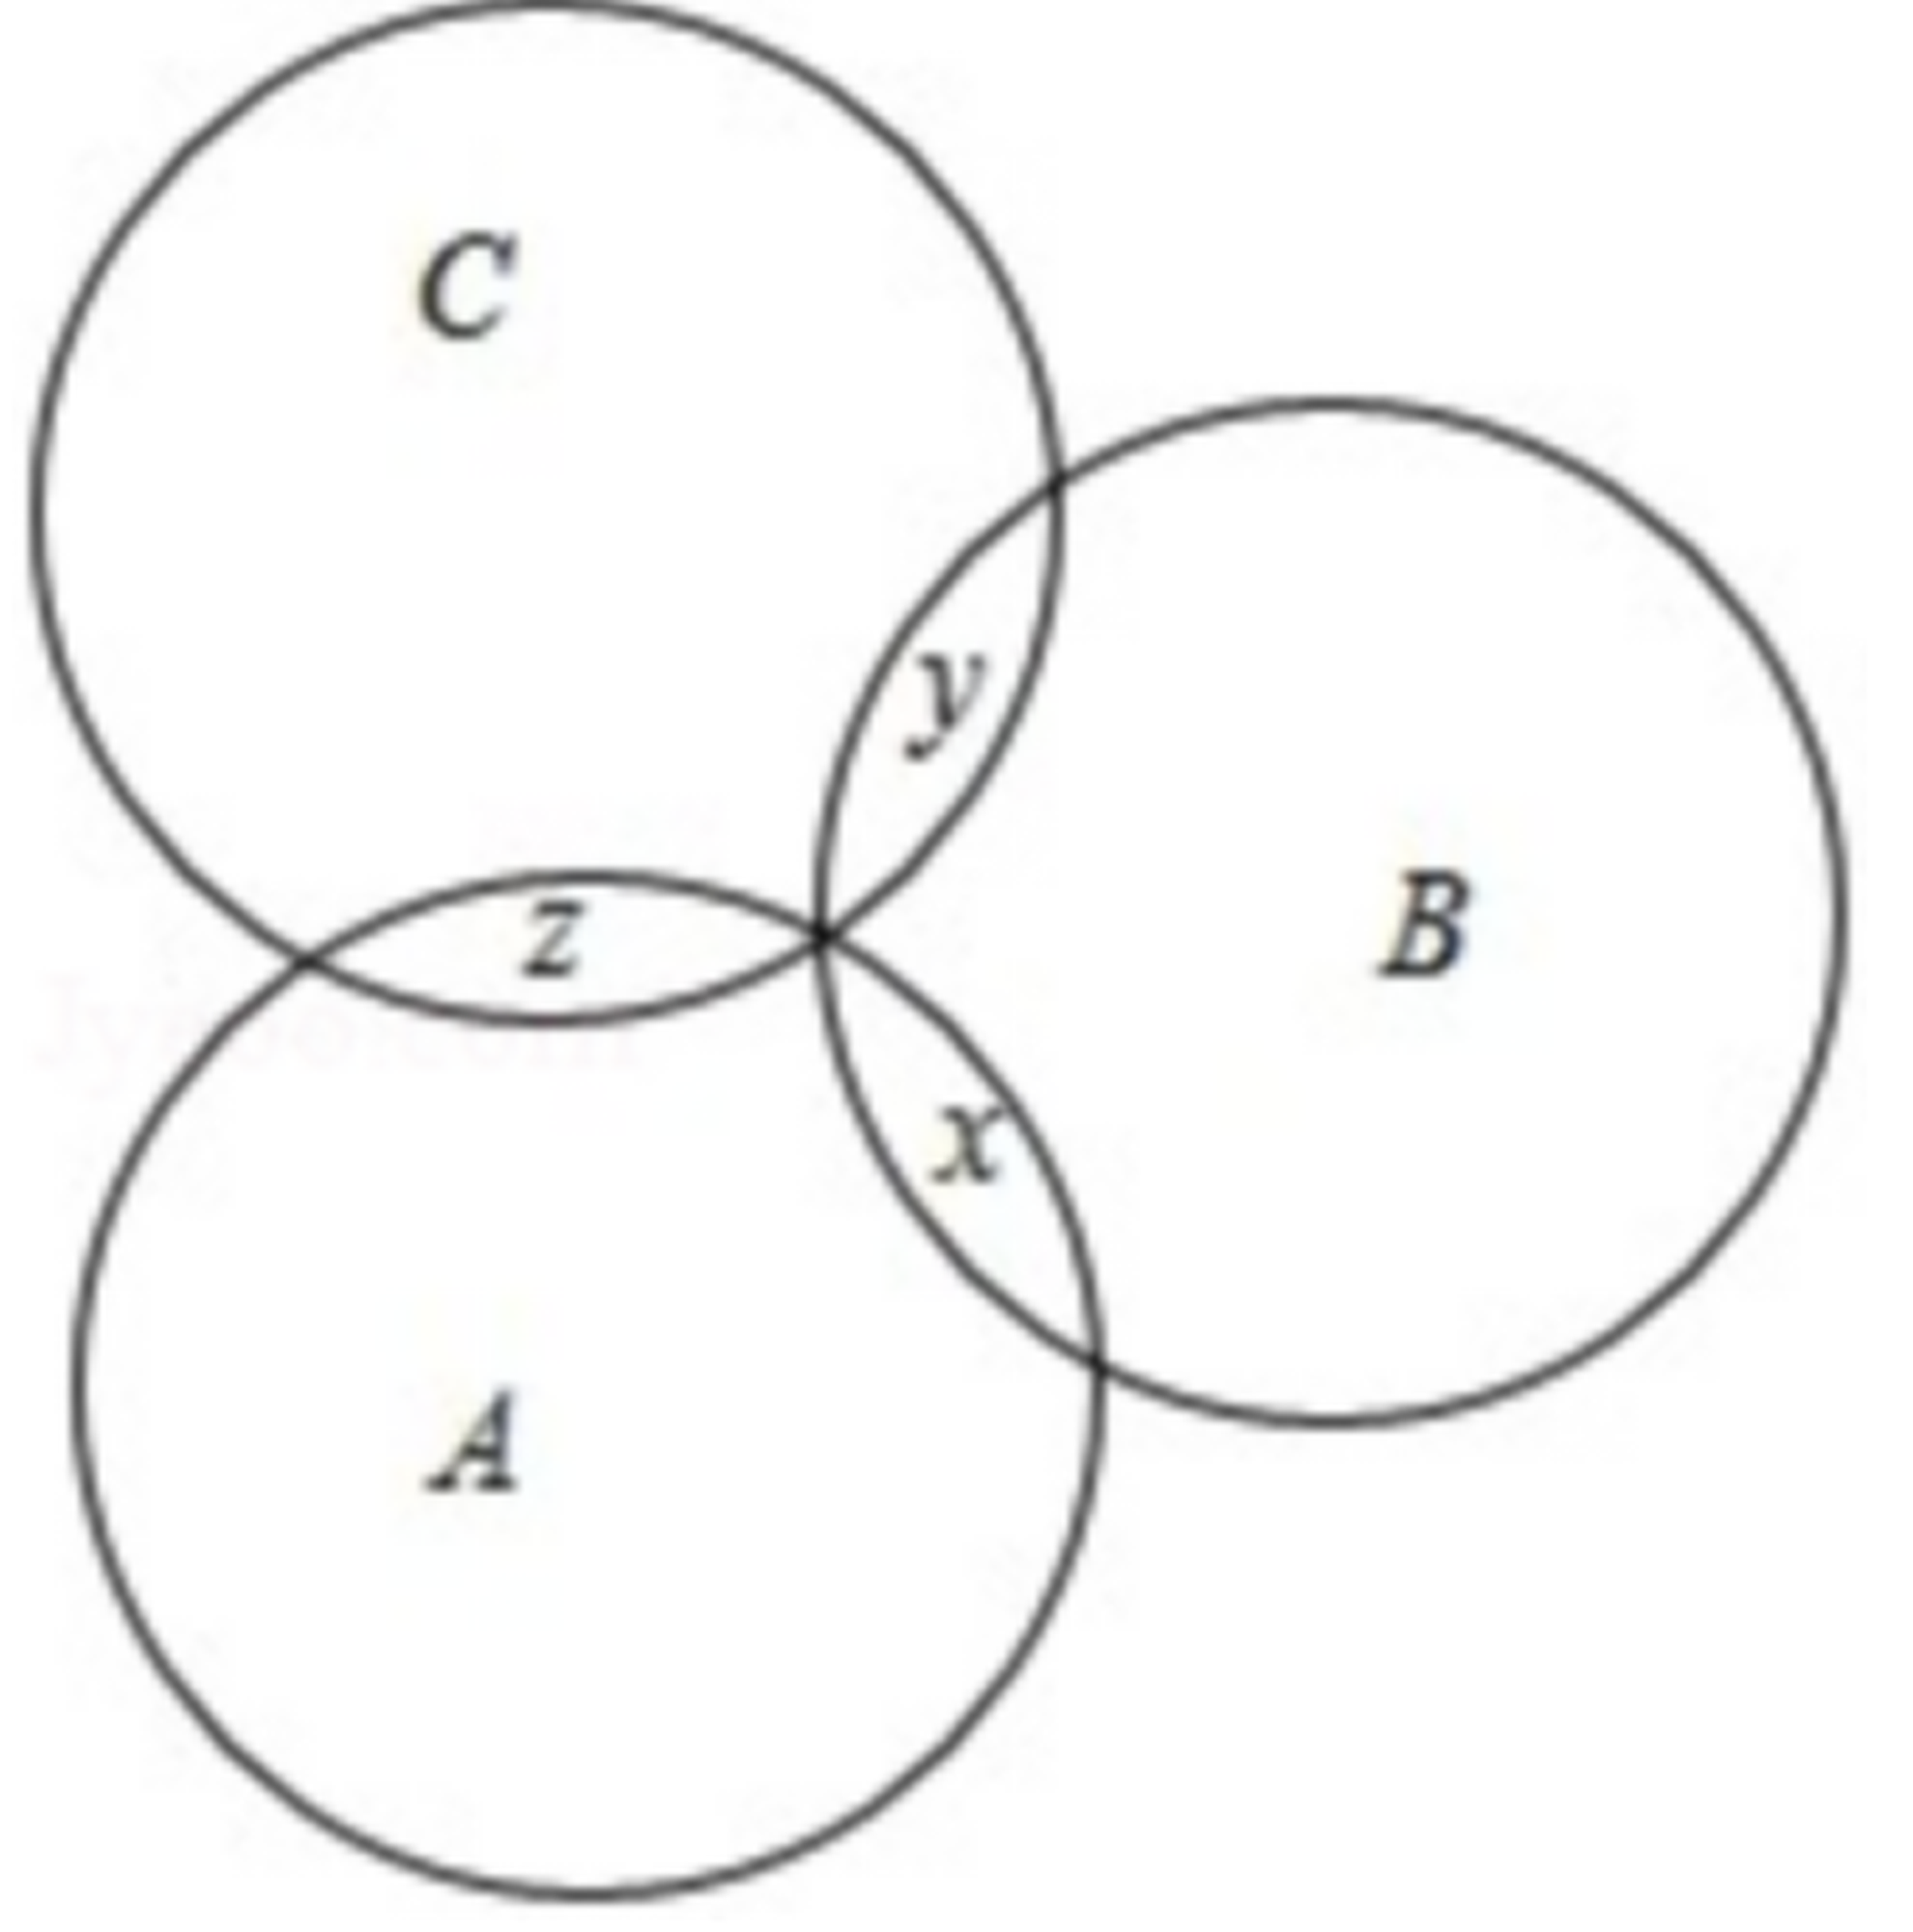
\includegraphics[width=0.30\textwidth]{figures/venn_ABC_x_y_z_h39.png}
\end{center}
\step{因为 $|A\cap B|=|B\cap C|=|C\cap A|=1$，且 $x$、$y$、$z\in\{1,2,3\}$，}
\step{所以集合 $A=\{x,z\}$，$B=\{x,y\}$，$C=\{z,y\}$，}
\step{若 $x=1$，$y=2$，$z=3$，则 $A=\{1,3\}$，$B=\{1,3\}$，$C=\{2,3\}$，}
\step{将 $1$，$2$，$3$ 进行全排列，有 $P_3^3=3\times2=6$ 个.}
\solend

\fi

\item 已知集合 $T=\{1,2,\cdots,2025\}$，对于 $T$ 的每一个非空子集的所有元素，计算它们乘积的倒数，
则所有这样倒数的和为 \blankline[4.4em].

\ans{$2025$}

\ifanswer
\solbegin
\step{集合 $T=\{1,2,\cdots,2025\}$ 的非空子集的个数为 $2^{2025}-1$，}
\step{这些子集中，每个元素的乘积分别为}
\step{$1,2,3,\cdots,2025,1\times2,1\times3,\cdots,1\times2025,\cdots,1\times2\times3\times\cdots\times2025$，}
\step{每项都可以看作是从 $1,2,3,\cdots,2025$ 中选择若干项的乘积，}
\step{$1+\dfrac12+\cdots+\dfrac{1}{2025}+\dfrac{1}{1\times2}+\dfrac{1}{1\times3}+\cdots+\dfrac{1}{2024\times2025}
+\cdots+\dfrac{1}{1\times2\times\cdots\times2025}$}
\step{$=(1+1)\left(1+\dfrac12\right)\cdots\left(1+\dfrac{1}{2025}\right)-1
=2\times\dfrac32\times\dfrac43\times\cdots\times\dfrac{2026}{2025}-1=2025$.}
\solend

\fi

% 第 24 题是压轴题，题干较长；试卷版在它之前量一次页高，尽量不与前文分家（照全稿成例）。
\ansneed{5cm}
% 注：原卷【解析】①③ 两步把 $f(x)$ 印作 $f[x[x]]$，显系笔误，照录未改，见文件头「笔误/存疑」⑦。
\item 若 $X$ 是一个集合，$T$ 是一个以 $X$ 的某些子集为元素的集合，且满足：①$X$ 属于 $T$，
$\varnothing$ 属于 $T$；②$T$ 中任意多个元素的并集属于 $T$；③$T$ 中任意多个元素的交集属于 $T$.
则称 $T$ 是集合 $X$ 上的一个拓扑. 已知函数 $f(x)=[x[x]]$，其中 $[x]$ 表示不大于 $x$ 的最大整数，
当 $x\in(0,n]$，$n\in\N^*$ 时，函数 $f(x)$ 值域为集合 $A_n$，则集合 $A_2$ 上的含有 $4$ 个元素的
拓扑 $T$ 的个数为 \blankline[4.4em].

\ans{$9$}

\ifanswer
\solbegin
\step{由题意，$n=2$，故 $0<x\leqslant2$，}
\step{①当 $0<x<1$ 时，则 $[x]=0$，所以 $f[x[x]]=0$，}
\step{②当 $x=1$ 时，$[x]=1$ 显然 $f(1)=1$，}
\step{③当 $1<x<2$ 时，$[x]=1$，所以 $f[x[x]]=[x]=1$，}
\step{④当 $x=2$ 时，$f(2)=4$，}
\step{所以 $A_2=\{0,1,4\}$，}
\step{因为 $T$ 中含有 $4$ 个元素，其中两个元素 $\varnothing$ 和 $A_2$，}
\step{$A_2=\{0,1,4\}$. 其它两个元素为 $A$、$B$，则
$\begin{cases}A\neq\varnothing\\ A\neq A_2\\ B\neq\varnothing\\ B\neq A_2\\ A\neq B\end{cases}$，}
\step{由对称性，不妨设 $1\leqslant|A|\leqslant|B|\leqslant2$，其中 $|A|$、$|B|$ 表示集合 $A$ 中元素的个数，}
\step{因为 $\begin{cases}A\cap B\in T\\ A\cup B\in T\end{cases}$，又 $|A|\leqslant|B|$，所以 $A\cap B=\varnothing$ 或 $A$，}
\step{若 $A\cap B=\varnothing$，则 $A\cup B$ 只能等于 $A_2$，}
\step{（若 $A\cup B=B$，则 $A\sub B$，则 $A\cap B=A=\varnothing$，矛盾）}
\step{则必有 $\begin{cases}|A|=1\\ |B|=2\end{cases}$，所以 $(A,B)$ 的个数 $\Leftrightarrow$ $A$ 的个数 $=3$ 种，}
\step{即 $\begin{cases}A=\{0\}\\ B=\{1,4\}\end{cases}$ 或 $\begin{cases}A=\{1\}\\ B=\{0,4\}\end{cases}$
或 $\begin{cases}A=\{4\}\\ B=\{0,1\}\end{cases}$；}
\step{若 $A\cap B=A\Leftrightarrow A\sub B$ 此时满足 $A\cup B=B$，}
\step{因为 $A\neq B$ 且 $1\leqslant|A|$ 且 $|B|\leqslant2$，所以 $\begin{cases}|A|=1\\ |B|=2\end{cases}$，}
\step{所以 $B$ 的选择共有 $C_3^2=3$ 种，则 $A$ 的个数有 $C_2^1$ 种，}
\step{所以 $(A,B)$ 的个数 $=2\times3=6$ 种.}
% 这六组「$A$／$B$」按原卷排作两行（前五个一行、第六个另起一行）；因五组并排时
% amsmath 的 cases 会为每组的第二列各留一枚 \quad，本行改排 \left\{\begin{matrix}…\end{matrix}\right.
% 以省下这枚 \quad（照 README「说明」记的高一07 成例），字形与 cases 相同。
\step{（这 $6$ 种是 $\left\{\begin{matrix}A=\{0\}\\ B=\{0,1\}\end{matrix}\right.$、
$\left\{\begin{matrix}A=\{1\}\\ B=\{0,1\}\end{matrix}\right.$、
$\left\{\begin{matrix}A=\{0\}\\ B=\{0,4\}\end{matrix}\right.$、
$\left\{\begin{matrix}A=\{4\}\\ B=\{0,4\}\end{matrix}\right.$、
$\left\{\begin{matrix}A=\{1\}\\ B=\{1,4\}\end{matrix}\right.$、}
\step{$\left\{\begin{matrix}A=\{4\}\\ B=\{1,4\}\end{matrix}\right.$）.}
\step{综上，$T$ 的个数为 $9$ 个.}
\solend

\fi

\end{enumerate}

\end{document}
"
%
% 原始材料是微信公众号图文（公众号「魔都数学加油站」连载「27学年高一 39」，署名「破晓」，
% 2026-09-26 21:29 发布，原文标题「27学年高一39——2026-2027年上海市大同中学高一上周末作业4.1」，
% 原文链接 https://mp.weixin.qq.com/s/HR2hIayXUXNi4zTs3PioiQ ），正文为 11 张 PNG 页。**同一篇里各页分辨率不一致**（2560×3620 与 4762×6735 两档混排：第 1、3、8、10 页为
% 2560×3620，第 2、4、5、6、7、9、11 页为 4762×6735）。原文本身就是一份**讲评版**——除第 15 题
% 外各题题下直接印【解析】（无单独的【答案】行），第 15 题的答案「D」直接印在题干末尾的括号内。
% 试题文字、答案与解析均照原卷录入，未改内容。卷面的粉色斜水印「魔都数学加油站」属水印，未录入。
%
% 卷首标题：原卷页首印作「2026-2027 年大同中学高一上周末作业 4.1」（**卷面标题行即带校名**，
% 年份区间按全稿惯例排 en dash，前缀照原卷保留「年」）。
%
% 篇幅与题号：卷面自「一、填空题」的**第 3 题**起编，终于「附加题」的**第 24 题**，共 22 题
% （填空 3—12、选择 13—16、解答 17—20、附加题 21—24）。第 1、2 题未在该文中发布——这是该
% 公众号连载讲评版的通例（高一02—高一09 等均自第 3 题起编，README「说明」已记），**不是截断**，
% 故本稿题号亦自 3 起。它与 高一40（大同中学 周末作业4.2）同属「周末作业 4」系列但**各自独立起编**
% （4.2 自第 3 题起、终于第 19 题），不是同一份试卷的两半。
%
% 与原卷的排版差异（均已在 README「说明」中交代）：
%   ① 原文自**第 3 题**起（第 1、2 题未在该文中发布），故本稿题号亦自 3 起，填空题以
%      \setcounter{enumi}{2} 起编；选择、解答、附加题三节各按上一节末号另设 \setcounter
%      （选择题 \setcounter{enumi}{12}、解答题 \setcounter{enumi}{16}、附加题 \setcounter{enumi}{20}）；
%   ② 原卷本就印有「一、填空题」「二、选择题」「三、解答题」三节标题，末节印作「附加题」
%      （**不带「四、」**，且题号 21—24 续前编、不另起），本稿照原卷分节，只把标题改排成全稿
%      统一的「大节标题」样式；
%   ③ 原卷是「讲评版」：除第 15 题外，各题题下均印【解析】（**全卷无一条独立的【答案】行**）；
%      第 15 题无解析，答案「D」直接印在题干末尾的括号内。本稿统一改为试卷版隐去、答案版以
%      \ans{}／\ifanswer 块给出，两版彻底分离；原卷写在【解析】末句的结果，本稿照 高一38
%      （同校同系列、同为讲评版）的成例另提为 \ans{}；
%   ④ 数集记号原卷两套并用：实数集作斜体的 $R$（第 7、11、14、17、18、19 题），整数集作斜体
%      $Z$（第 10 题），自然数集作斜体 $N$ 及 $N^*$（第 16、20、21、24 题），本稿按全稿惯例
%      统一写作 $\R$、$\Z$、$\N$、$\N^*$；
%   ⑤ 补集符号原卷两套并用：第 7 题作前缀式的 $C_U$（且题干称全集为 $I$，见「笔误/存疑」①），
%      第 14、15、18 题作上横线（$\overline{H}$、$\overline{A}$、$\overline{B}$），本稿照录、不归一
%      （前缀式写作 $\complement_U$，与 高一c／高一10 的成例一致）；
%   ⑥ 包含符号原卷两套并用：第 3 题作**无下划线**的 $\subset$，第 15、18、20、24 题作**带下划线**
%      的 $\sub$，本稿照录、不归一；
%   ⑦ 原卷填空的横线约两个字宽，本稿按全稿惯例统一排 \blankline[4.4em]；
%   ⑧ 第 7、11、22 题各有插图，取原卷截图、4× LANCZOS 放大（figures/venn_N_cap_CI_M_h39.png、
%      figures/plane_grid_4squares_h39.png、figures/venn_ABC_x_y_z_h39.png）；第 7 题的 Venn 属
%      **题干**（试卷版、答案版都出），第 11、22 题的图在【解析】内（仅答案版出）。第 7 题图
%      左下、第 11 题图的上／左／右边缘带进极淡的原卷粉色水印残影——照全稿「插图直接取自
%      原卷截图、不用 TikZ 重绘、不修图」的体例保留（再裁会切到坐标轴与 $x$、$y$、$O$ 标注）；
%   ⑨ 原卷并列的字母、数字（「$x_1,x_2$」「$a,b$」「$1,2,3,\cdots,11$」）多作半角逗号或不加标点，
%      本稿按全稿惯例改排顿号（$x_1$、$x_2$）或把数列并入行内公式；半角括号、逗号一律排全角，
%      数学式内部的标点照原样；
%   ⑩ 原卷未印副标题，本稿按**本卷实际内容**补出副标题「集合与常用逻辑用语」（依据见下条）。
%
% 副标题（\examtitlest 第二个参数）：本卷卷面未印副标题，由本稿补出，取值按 2026-09-26 起的
%   新口径「只用本卷实际内容的模块名」定为「集合与常用逻辑用语」。依据：全卷 22 题（第 3—24 题）中，
%   第 3、5、7、8、10、11、14、15、16、17、18、19、20、21、22、23、24 题共 17 题是集合的运算与
%   关系、子集／真子集、补集、集合新定义（「全食／偏食」、最小相交、拓扑、特征数）与集合计数，
%   以及命题与常用逻辑用语（第 3 题充要条件、第 5 题存在量词命题、第 17 题命题真假）；其余两题
%   第 4、6 考一元二次方程的根（韦达定理）与方程恒等，第 9、12、13 题是不等式（一元二次不等式组
%   的整数解、一元二次不等式解集、不等式的性质）——不等式合计 3/22，**不足全卷三分之一**，
%   故不并标「不等式」。
%
% 原卷笔误/存疑（均照抄原卷、未改，见源码中该处上方注释）：
%   ① 第 7 题题干称「全集 $I=R$」，而【解析】两处把补集写作 $C_U M$（下标作 $U$），前后记号不一；
%      本稿照录，未改；
%   ② 第 4 题【解析】两处把判别式印作 $\triangle=[2(m-1)^2-16m^2]$（方括号内首项漏了平方，
%      正确应作 $[2(m-1)]^2-16m^2$）；按其所判「$m=\frac12$ 时 $<0$、$m=-\frac12$ 时 $>0$」反推，
%      $[2(m-1)]^2-16m^2$ 在 $m=\frac12$ 时为 $-3<0$、在 $m=-\frac12$ 时为 $5>0$，与结论一致；
%      本稿照录；
%   ③ 第 9 题【解析】把方程组第二式印作 $1-2<-k\leqslant3$，按其结论 $-3\leqslant k<2$ 反推，
%      疑当作 $-2<-k\leqslant3$（原卷多一个「$1$」）；本稿照录；
%   ④ 第 17 题【解析】首句「由数 $y=-x^2+ax-1=-x+3$」中的「由数」显系「由」或「由函数」之误；
%      且末段「若 $p$ 真 $q$ 假…得 $a\in R$」「若 $p$ 假 $q$ 真…此时 $a$ 无解」与结论「$a$ 的取值范围
%      是 $R$」自相矛盾（按 $p:a\leqslant-5$、$q:a>-6$，$p$ 真 $q$ 假应为 $a\leqslant-6$，$p$ 假 $q$ 真
%      应为 $a>-5$，合起来是 $a\leqslant-6$ 或 $a>-5$，并非 $R$）；本稿一律照录，未按正确解法改写；
%   ⑤ 第 18 题【解析】(2) 把 $B=\{x\mid x^2+a\leqslant0\}$（$a<0$）印作右端开的
%      $\{x\mid-\sqrt{-a}\leqslant x<\sqrt{-a}\}$（应为闭的「$\leqslant$」）；按其所判
%      $\sqrt{-a}<\frac12$ 反推，不影响结论；本稿照录；
%   ⑥ 第 22 题【解析】在 $x=1$、$y=2$、$z=3$ 时把 $B=\{x,y\}$ 印作 $\{1,3\}$（应为 $\{1,2\}$），
%      与本行前面「$B=\{x,y\}$」不合；本稿照录；
%   ⑦ 第 24 题【解析】①③ 两步把 $f(x)$ 印作 $f[x[x]]$，显系笔误；本稿照录。
%   ⑧ 第 8 题【解析】「即方程 $x^2+ax+b=x$，$x^2+(a-1)x+b=0$ **由**两个相等的实数根为 $4$」——
%      「由」当为「有」（「设…是…有」的杂糅）；本稿照录；
%   ⑨ 第 10 题：题设 $a\oplus b=b(a^2+b^2+1)$，而集合定义里含 $\dfrac{a\oplus b}{2b}$；$-2<a<b<2$、
%      $a$、$b\in\Z$ 时 $(a,b)=(-1,0)$ 也合条件、却使分母 $2b=0$，原卷解析仍代入该组并约去
%      $b$ 得 $x=1$（答案集恰好不变）；本稿照录；
%   ⑩ 第 15 题选项列里 ② 与 ③ 之间**漏排分隔号**（原卷作「② $\overline{A}\cap B=\varnothing$③
%      $\overline{A}\sub\overline{B}$；」——①、③ 后都有「；」，② 后没有）；本稿照录；
%   ⑪ 第 20(2) 把 $\{1,2,\cdots,20\}$ 分成的 11 个集合里，$\{8,11\}$ 与 $\{9,12\}$ 之间误用
%      **句号**「.」（同行其余处皆逗号）；本稿照录；
%   ⑫ 第 20(3)① 推理不严：原卷写「选 5 则不选 1、9；选 6 则不选 2、10；选 7 则不选 3、11；
%      则只剩 4、8」——但 4 与 8 相差 $4$、不能同选，该情形实际最多只能取 $4$ 个；末句结论
%      「不超过 $5$ 个」仍成立；本稿照录；
%   ⑬ 第 16 题【解析】两种下标并存：「所以在 $A_i$ 的特征数构成中」原卷作斜体 $A_i$，而
%      「要使 $X_1+X_2+X_3$ 最大（小），则（应）在集合 $A_1$ 中首先放置…」两处原卷作
%      **数字 $1$**（与同句 $X_1$ 的角标同形）；本稿照录、未归一。
%
% 图取原卷截图（依次见各处的 \includegraphics 前的注释），4× LANCZOS 放大。
\documentclass[a4paper,11pt]{article}
\usepackage{common}

\begin{document}

\examtitlest[3]{2026--2027 年大同中学高一上周末作业 4.1}{集合与常用逻辑用语}

\bigsec{一、填空题}

\begin{enumerate}
\setcounter{enumi}{2}

\item “$x\geqslant a$”是“$0<x<2$”的必要非充分条件，则实数 $a$ 的取值范围是 \blankline[4.4em].

\ans{$(-\infty,0]$}

\ifanswer
\solbegin
\step{因为 $x\geqslant a$ 是 $0<x<2$ 的必要非充分条件，所以 $(0,2)\subset[a,+\infty)$，所以 $a\leqslant0$，}
\step{则实数 $a$ 的取值范围是 $(-\infty,0]$.}
\solend

\fi

% 注：原卷$[2(m-1)^2-16m^2]$ 首项漏了平方（应为 $[2(m-1)]^2-16m^2$），照录未改，见文件头「笔误/存疑」②。
\item 若关于 $x$ 的方程 $x^2+2(m-1)x+4m^2=0$ 有两个实数根，且这两根互为倒数，则 $m=$ \blankline[4.4em].

\ans{$-\dfrac12$}

\ifanswer
\solbegin
\step{设 $x_1$、$x_2$ 是方程 $x^2+2(m-1)x+4m^2=0$ 有两个实数根，}
\step{则 $x_1x_2=4m^2=1$，解得 $m=\dfrac12$ 或 $m=-\dfrac12$，}
\step{又当 $m=\dfrac12$ 时，$\triangle=[2(m-1)^2-16m^2]<0$，舍去，}
\step{当 $m=-\dfrac12$ 时，$\triangle=[2(m-1)^2-16m^2]>0$，故 $m=-\dfrac12$.}
\solend

\fi

\item 已知命题：“存在 $x\in[1,2]$，使 $x^2+2x+a\geqslant0$”为真命题，则 $a$ 的取值范围是 \blankline[4.4em].

\ans{$a\geqslant-8$}

\ifanswer
\solbegin
\step{若存在 $x\in[1,2]$，使 $x^2+2x+a\geqslant0$，}
\step{则等价为存在 $x\in[1,2]$，使 $x^2+2x\geqslant-a$，}
\step{当存在 $x\in[1,2]$ 时，设 $y=x^2+2x=(x+1)^2-1$，则 $3\leqslant y\leqslant8$，}
\step{所以要使 $x^2+2x\geqslant-a$，则 $8\geqslant-a$，即 $a\geqslant-8$.}
\solend

\fi

\item 已知方程 $a(3x+2)+b(2x-3)=8x+3$ 有无穷多个解，则 $a:b=$ \blankline[4.4em].

\ans{$30:7$}

\ifanswer
\solbegin
\step{$a(3x+2)+b(2x-3)=(3a+2b)x+2a-3b=8x+3$ 有无穷多个解，}
\step{所以 $\begin{cases}3a+2b=8\\ 2a-3b=3\end{cases}$，解得 $a=\dfrac{30}{13}$，$b=\dfrac{7}{13}$，所以 $a:b=30:7$.}
\solend

\fi

% 注：原卷题干称「全集 $I=R$」，而【解析】两处把补集写作 $C_U M$（下标作 $U$），前后记号不一；
%     照录未改，见文件头「笔误/存疑」①。
\item 已知集合 $M=\{x\mid y=\sqrt{3-x^2}\}$，$N=\{x\mid-3\leqslant x\leqslant1\}$，全集 $I=\R$，
则图中阴影部分表示的集合为 \blankline[4.4em].

% 图取原卷截图（01.png，2560×3620）右栏，4× LANCZOS 放大。
\begin{center}
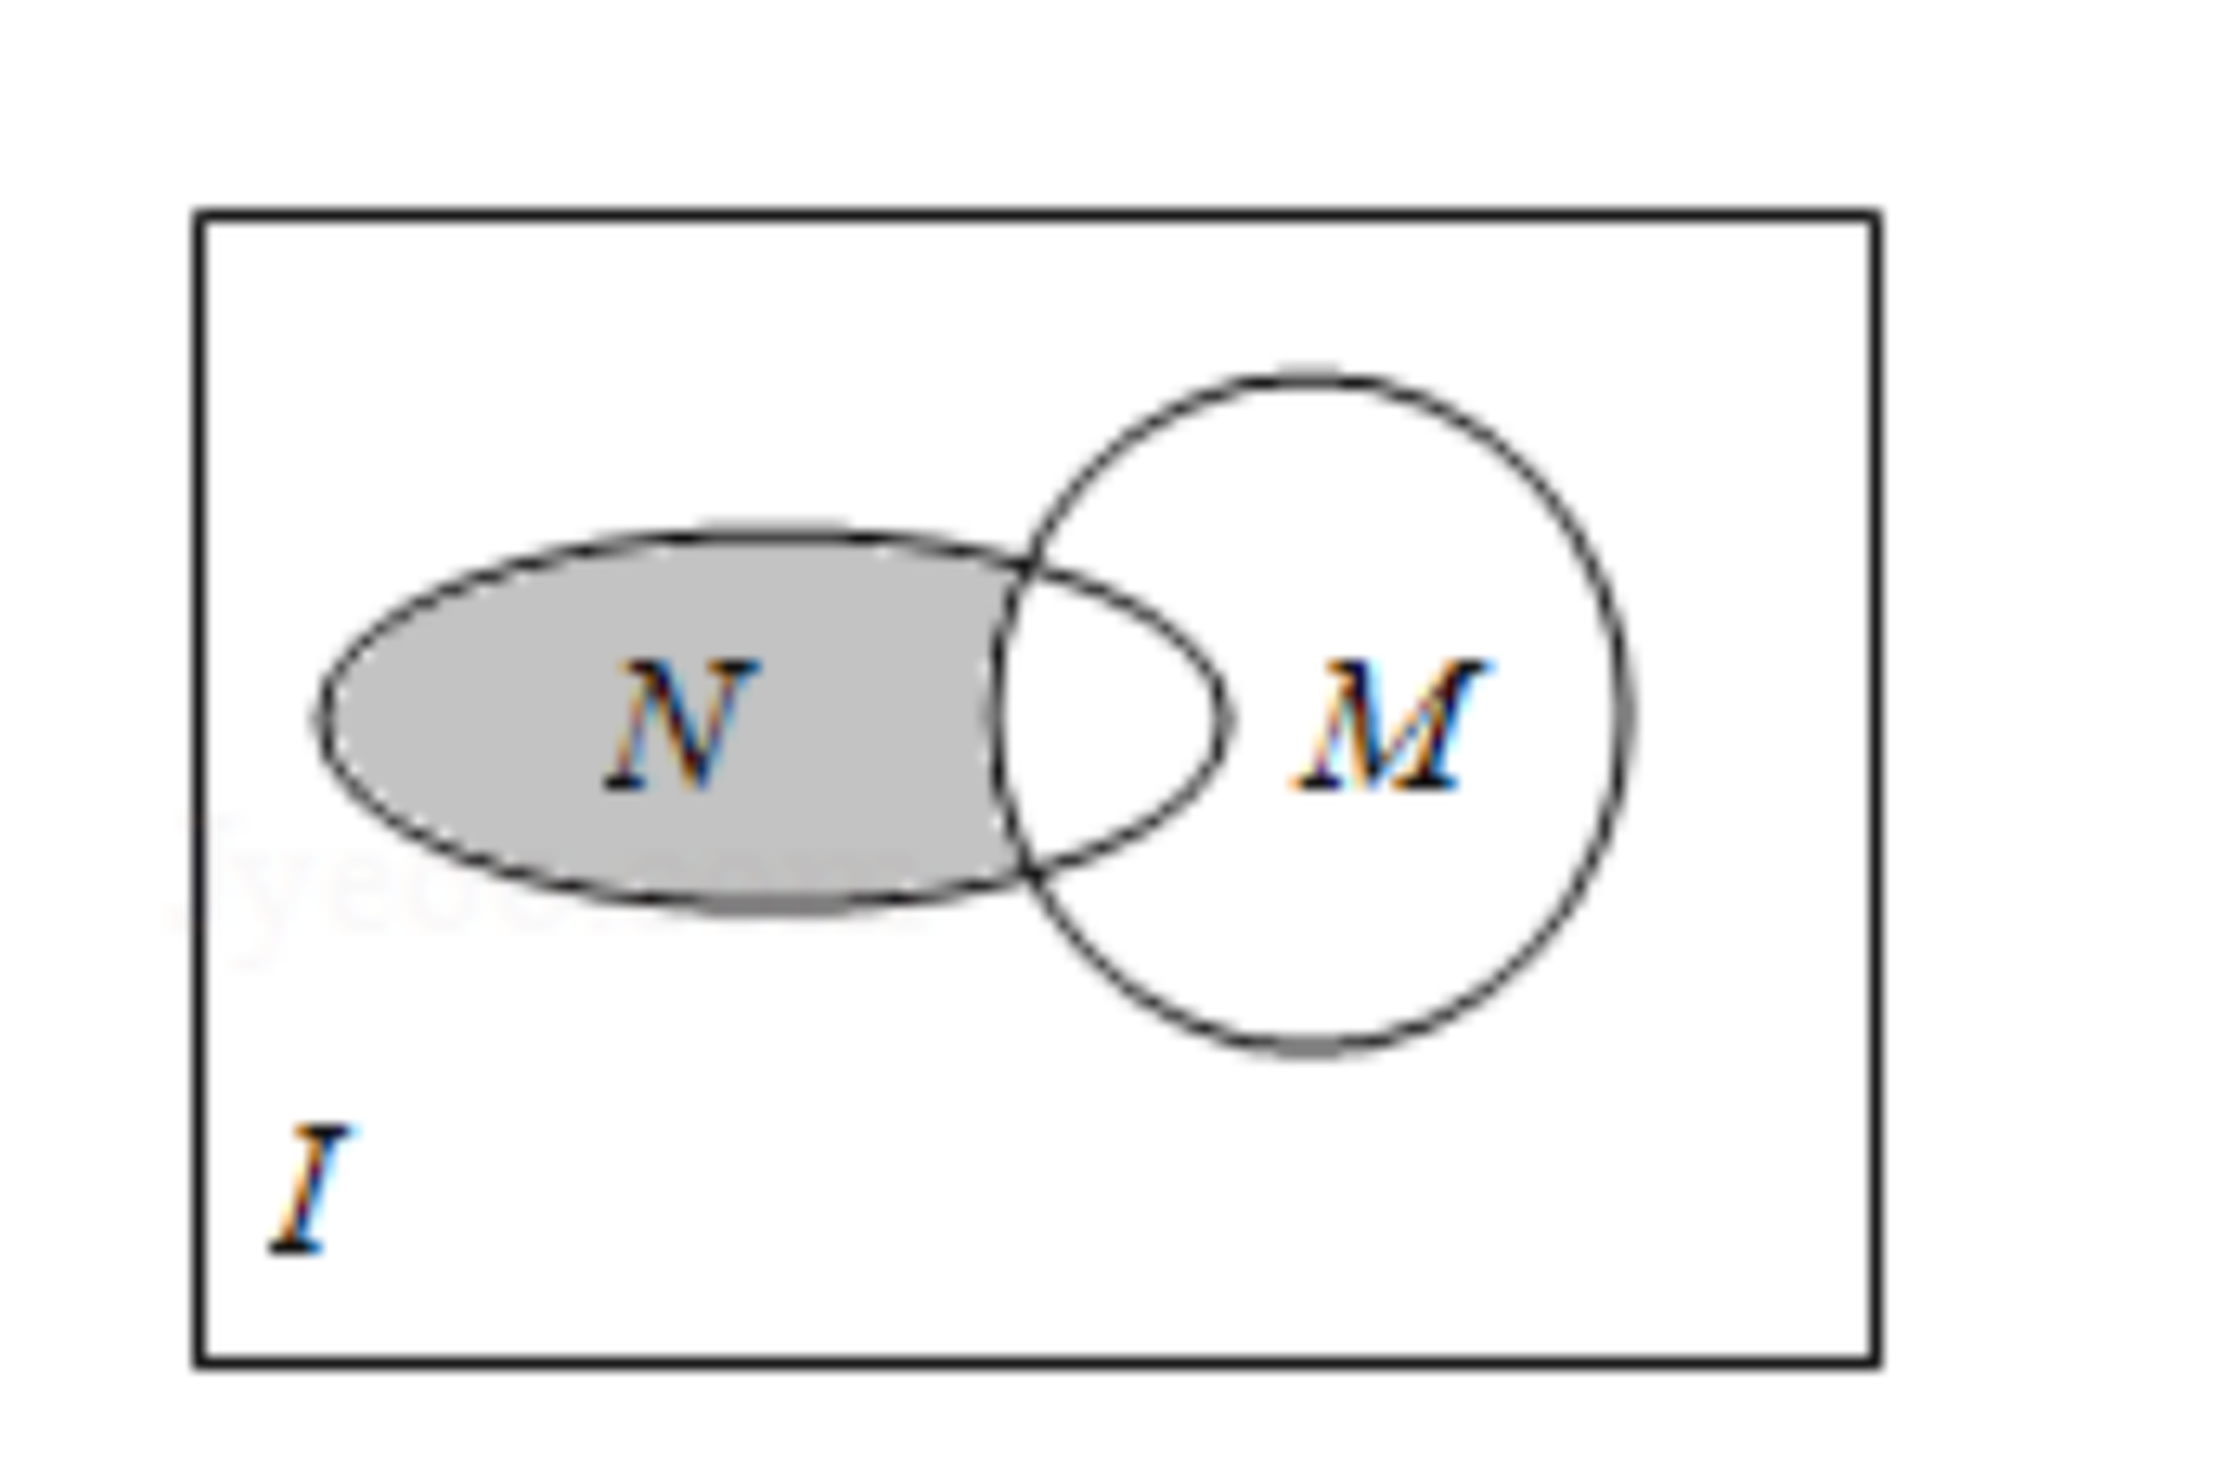
\includegraphics[width=0.30\textwidth]{figures/venn_N_cap_CI_M_h39.png}
\end{center}

\ans{$[-3,-\sqrt3)$}

\ifanswer
\solbegin
\step{阴影部分用集合表示为 $N\cap(\complement_UM)$.}
\step{则 $M=\{x\mid y=\sqrt{3-x^2}\}=\{x\mid3-x^2\geqslant0\}=\{x\mid-\sqrt3\leqslant x\leqslant\sqrt3\}$，}
\step{则 $\complement_UM=\{x\mid x>\sqrt3\text{ 或 }x<-\sqrt3\}$，$N=\{x\mid|x+1|\leqslant2\}=\{x\mid-3\leqslant x\leqslant1\}$，}
\step{则 $N\cap(\complement_UM)=\{x\mid-3\leqslant x<-\sqrt3\}$.}
\solend

\fi

\item 已知 $f(x)=x^2+ax+b$，集合 $\{x\mid f(x)=x\}=\{4\}$，将集合 $M=\{x\mid f(x)=4\}$ 用列举法表示 \blankline[4.4em].

\ans{$\{3,4\}$}

\ifanswer
\solbegin
\step{已知 $f(x)=x^2+ax+b$，集合 $\{x\mid f(x)=x\}=\{4\}$，}
% 注：原卷本行作「…$x^2+(a-1)x+b=0$ **由**两个相等的实数根为 $4$」——「由」当为「有」
%     （「设…是…有」的杂糅）；本稿照录未改，见文件头「原卷笔误/存疑」⑧。
\step{即方程 $x^2+ax+b=x$，$x^2+(a-1)x+b=0$ 由两个相等的实数根为 $4$，}
\step{所以 $\triangle=(a-1)^2-4b=0$，即 $x^2+(a-1)x+b=(x-4)^2$，所以 $b=16$，$a=-7$，}
\step{所以 $f(x)=x^2+ax+b=x^2-7x+16$，所以集合 $M=\{x\mid f(x)=4\}$，}
\step{即 $x^2-7x+16=4$，$x^2-7x+12=0$，故 $M=\{x\mid f(x)=4\}=\{3,4\}$.}
\solend

\fi

% 注：原卷方程组第二式印作 $1-2<-k\leqslant3$，按其结论 $-3\leqslant k<2$ 反推疑当作 $-2<-k\leqslant3$，
%     照录未改，见文件头「笔误/存疑」③。
\item 关于 $x$ 的不等式组 $\begin{cases}x^2-x-2>0\\ 2x^2+(2k+5)x+5k<0\end{cases}$ 的整数解的集合为 $\{-2\}$，
则实数 $k$ 的取值范围 \blankline[4.4em].

\ans{$-3\leqslant k<2$}

\ifanswer
\solbegin
\step{原不等式组即 $\begin{cases}(x-2)(x+1)>0\\ (x+k)(2x+5)<0\end{cases}$，整数解的集合为 $A$，若 $A=\{-2\}$，}
\step{则 $(-2+k)(2\times(-2)+5)<0$，所以 $k<2$，且有 $\begin{cases}-k>-\dfrac52\\ 1-2<-k\leqslant3\end{cases}$，}
\step{解得 $-3\leqslant k<2$.}
\solend

\fi

\item 规定 $\oplus$ 与 $\otimes$ 是两个运算符号，其运算法则如下，对任意实数 $a$、$b$ 有：$a\otimes b=ab$，
$a\oplus b=b(a^2+b^2+1)$. 若 $-2<a<b<2$ 且 $a$、$b\in\Z$，
$A=\left\{x\mid x=2(a\otimes b)+\dfrac{a\oplus b}{2b}\right\}$，则用列举法表示集合 $A=$ \blankline[4.4em].

\ans{$\left\{1,-\dfrac12\right\}$}

\ifanswer
\solbegin
\step{$A=\left\{x\mid x=2(a\otimes b)+\dfrac{a\oplus b}{2b}\right\}
=\left\{x\mid x=2ab+\dfrac{b(a^2+b^2+1)}{2b}\right\}$}
\step{$=\left\{x\mid x=2ab+\dfrac12a^2+\dfrac12b^2+\dfrac12\right\}
=\left\{x\mid x=\dfrac12(a+b)^2+ab+\dfrac12\right\}$，}
% 注：题设含 $\dfrac{a\oplus b}{2b}$，而 $-2<a<b<2$、$a$、$b\in\Z$ 时 $(a,b)=(-1,0)$ 也合条件、
%     却使分母 $2b=0$；原卷解析仍代入该组并约去 $b$ 得 $x=1$（答案集恰好不变）。本稿照录，
%     见文件头「原卷笔误/存疑」⑨。
\step{当 $a=-1$，$b=0$ 时，$x=1$；当 $a=-1$，$b=1$ 时，$x=-\dfrac12$；}
\step{当 $a=0$，$b=1$ 时，$x=1$；所以 $A=\left\{1,-\dfrac12\right\}$.}
\solend

\fi

\item 高斯是德国著名的数学家，近代数学奠基者之一，享有“数学王子”的称号，为了纪念数学家高斯，
我们把取整函数 $y=[x]$，$x\in\R$ 称为高斯函数，其中 $[x]$ 表示不超过 $x$ 的最大整数，
如 $[1.1]=1$，$[-1.1]=-2$. 则点集 $P=\{(x,y)\mid[x]^2+[y]^2=1\}$
所表示的平面区域的面积是 \blankline[4.4em].

\ans{$4$}

\ifanswer
\solbegin
\step{$[x]^2+[y]^2=1$ 由 $\begin{cases}[x]=0\\ [y]=-1\end{cases}$ 或 $\begin{cases}[x]=0\\ [y]=1\end{cases}$
或 $\begin{cases}[x]=-1\\ [y]=0\end{cases}$ 或 $\begin{cases}[x]=1\\ [y]=0\end{cases}$ 四个平面区域组成，}
\step{即 $\begin{cases}0\leqslant x<1\\ -1\leqslant y<0\end{cases}$ 或 $\begin{cases}0\leqslant x<1\\ 1\leqslant y<2\end{cases}$
或 $\begin{cases}-1\leqslant x<0\\ 0\leqslant y<1\end{cases}$ 或 $\begin{cases}1\leqslant x<2\\ 0\leqslant y<1\end{cases}$，}
\step{作出平面区域如图所示，平面区域由四个边长为 $1$ 的正方形组成，}
% 图在【解析】内（仅答案版出），取原卷截图（03.png，2560×3620）中部，4× LANCZOS 放大。
\begin{center}
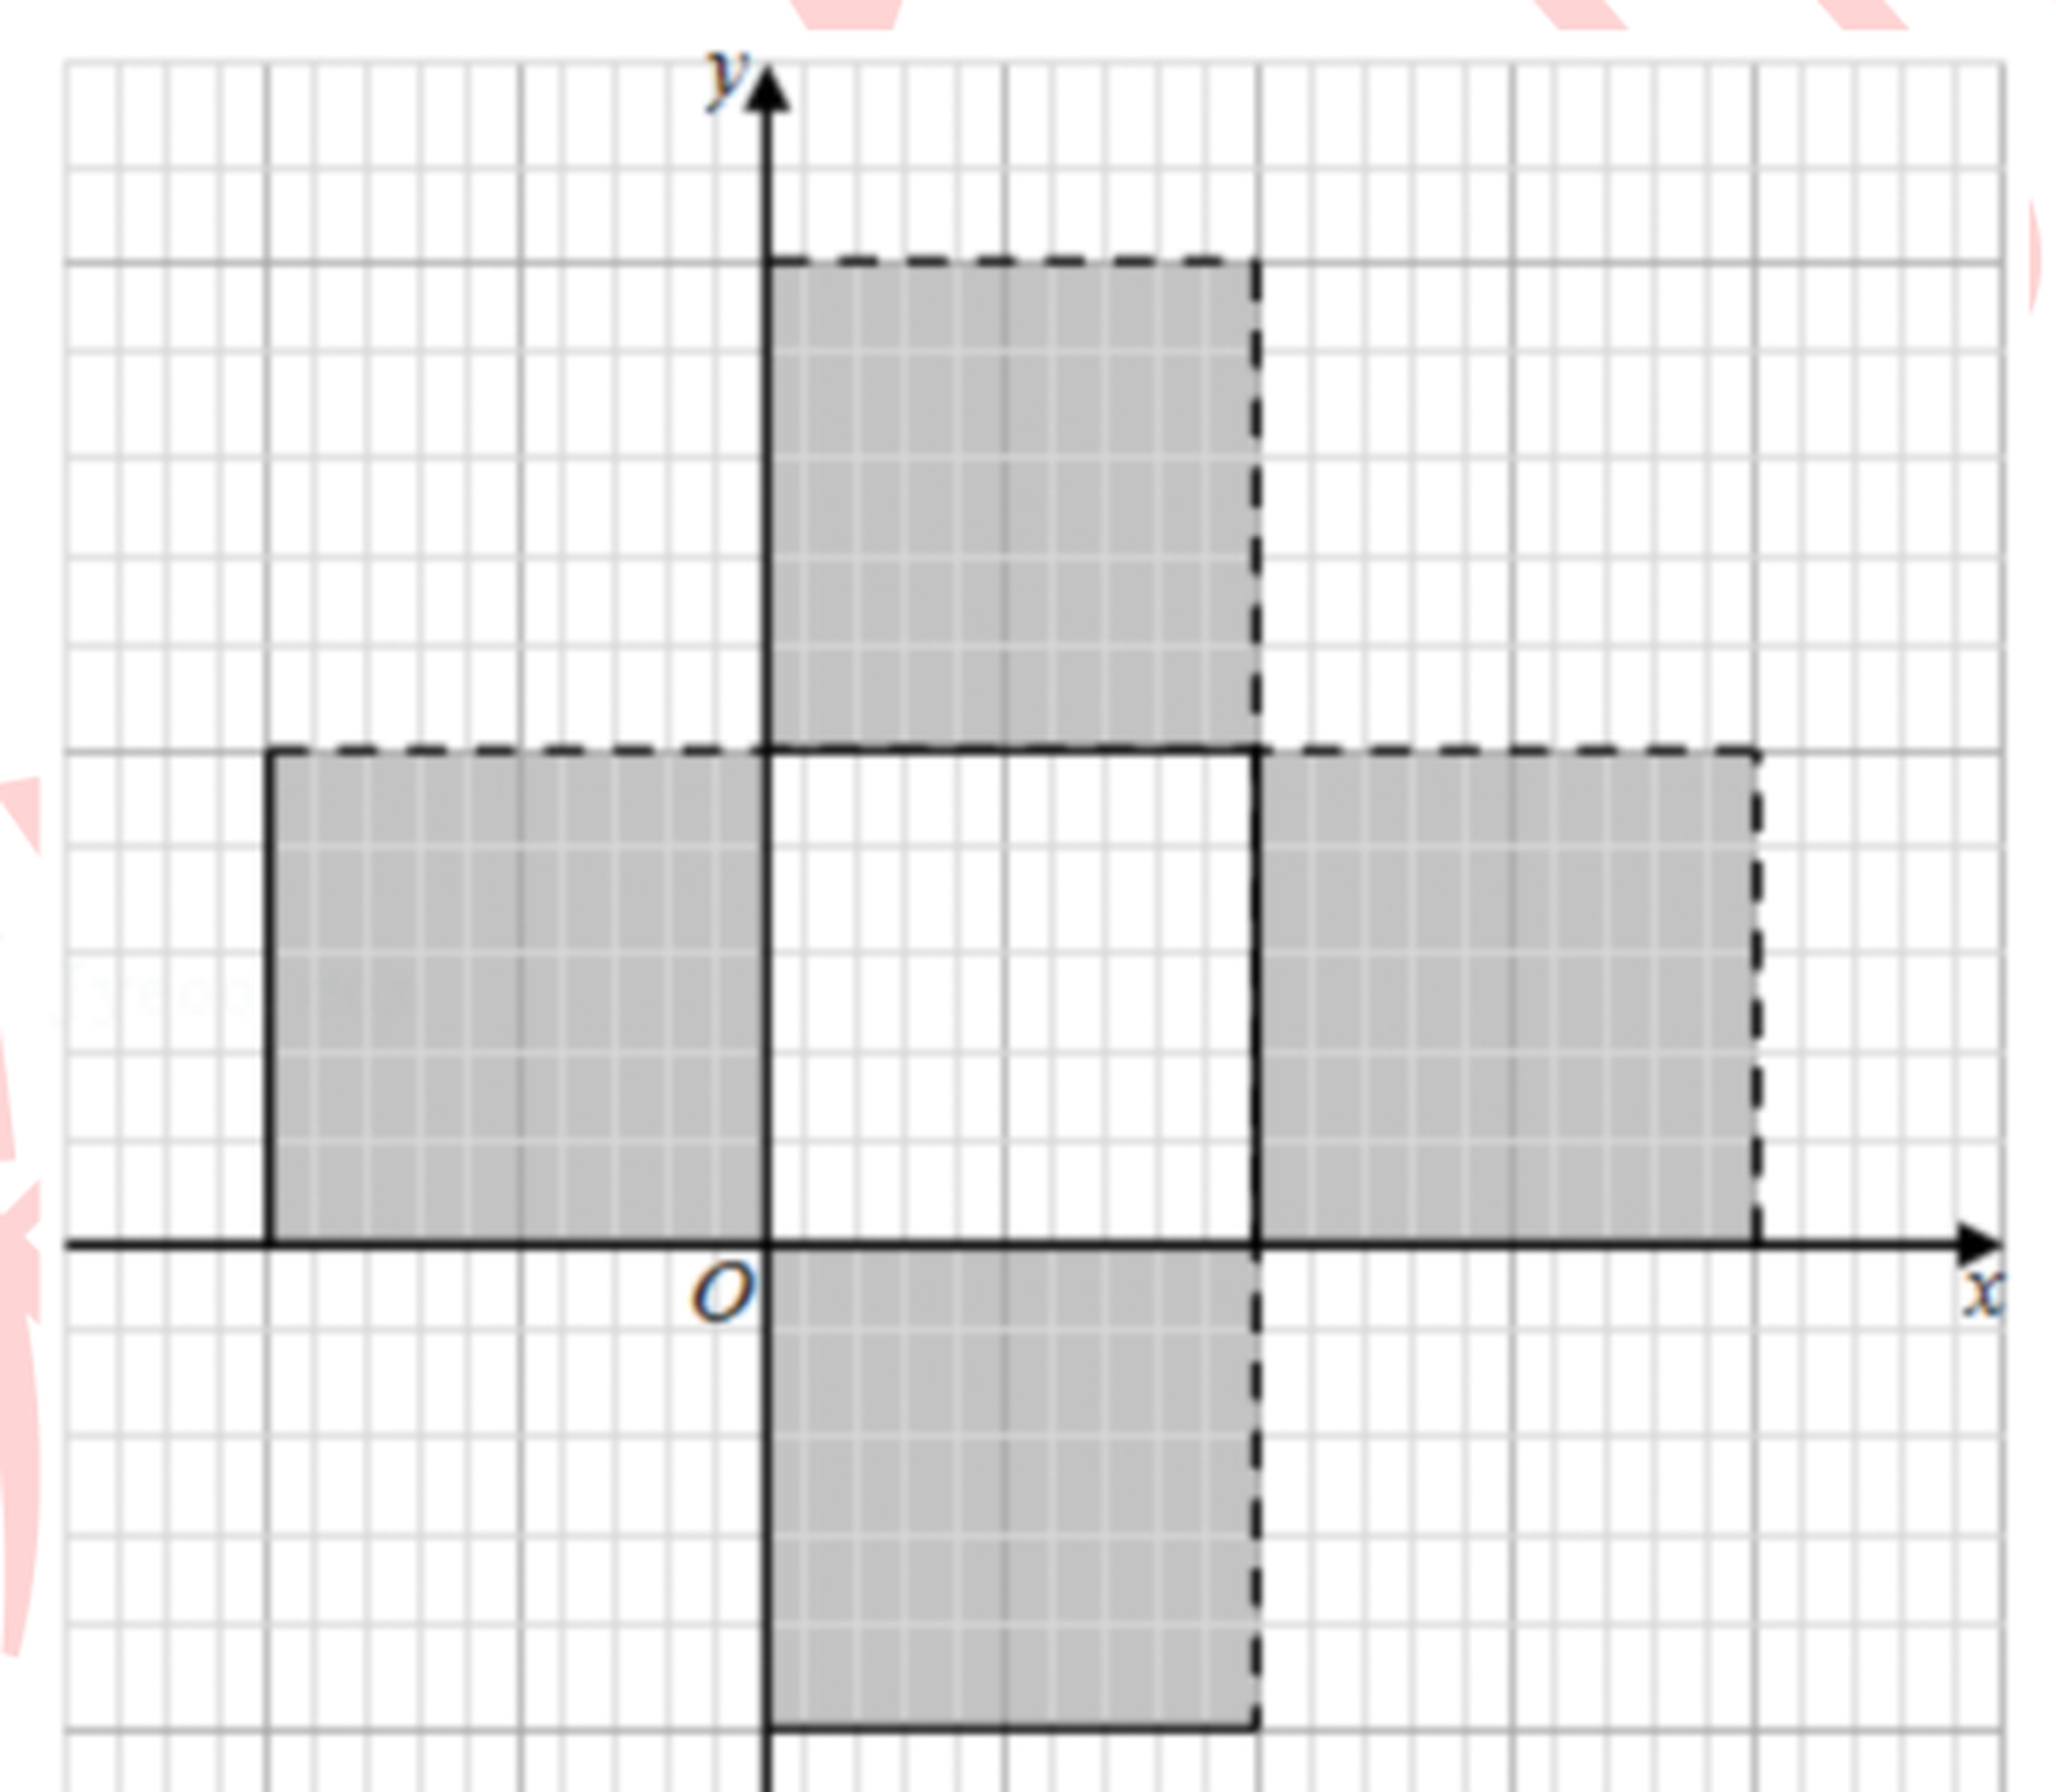
\includegraphics[width=0.38\textwidth]{figures/plane_grid_4squares_h39.png}
\end{center}
\step{总面积为 $1\times4=4$.}
\solend

\fi

\item 关于 $x$ 的不等式 $ax^2+bx+c>0$ 的解集为 $\{x\mid x<\beta\text{ 或 }x>\gamma\}(0<\beta<\gamma)$，
则不等式 $a(x^2+1)+b(x-1)+c>2ax$ 的解集为 \blankline[4.4em].

\ans{$(-\infty,\beta+1)\cup(\gamma+1,+\infty)$}

\ifanswer
\solbegin
\step{由题意得 $\beta$、$\gamma$ 为方程 $ax^2+bx+c=0$ 的两根且 $a>0$，}
\step{则 $\beta+\gamma=-\dfrac ba$，$\beta\gamma=\dfrac ca$，故 $b=-a(\beta+\gamma)$，$c=\beta\gamma a$，}
\step{则不等式可化为 $a(x^2+1)-a(\beta+\gamma)(x-1)+\beta\gamma a>2ax$，}
\step{因为 $a>0$，所以 $x^2+1-(\beta+\gamma)(x-1)+\beta\gamma>2x$，}
\step{即 $x^2-(\beta+\gamma+2)x+(\beta+\gamma+\beta\gamma+1)>0$，所以 $(x-\beta-1)(x-\gamma-1)>0$，}
\step{解得 $x<\beta+1$ 或 $x>\gamma+1$，所以不等式解集为 $(-\infty,\beta+1)\cup(\gamma+1,+\infty)$.}
\solend

\fi

\end{enumerate}

\bigsec{二、选择题}

\begin{enumerate}
\setcounter{enumi}{12}

\item 设 $a<b<0$，则下列不等式中不成立的是\mbox{（\quad）}

\keepwithprev
A. $\dfrac1a>\dfrac1b$\qquad B. $\dfrac{1}{a-b}>\dfrac1a$\qquad C. $|a|>-b$\qquad D. $\sqrt{-a}>\sqrt{-b}$

\ans{$B$}

\ifanswer
\solbegin
\step{令 $a=-2$，$b=-1$，}
\step{A、$-\dfrac12>-1$，正确；B、$-1<-\dfrac12$，故 B 错误；C、$2>1$，正确；}
\step{D、$\sqrt2>1$，正确；故选 B.}
\solend

\fi

\item 设实数集 $\R$ 为全集，集合 $P=\{x\mid f(x)=0\}$，$Q=\{x\mid g(x)=0\}$，$H=\{x\mid h(x)=0\}$，
则方程 $\dfrac{f^2(x)+g^2(x)}{h(x)}=0$ 的解集是\mbox{（\quad）}

\keepwithprev
A. $P\cap Q\cap\overline{H}$\qquad B. $P\cap Q$\qquad C. $P\cap Q\cap H$\qquad D. $P\cap Q\cup H$

\ans{$A$}

\ifanswer
\solbegin
\step{方程 $\dfrac{f^2(x)+g^2(x)}{h(x)}=0$ 等价于 $\begin{cases}f(x)=0\\ g(x)=0\\ h(x)\neq0\end{cases}$，}
\step{又因为 $P=\{x\mid f(x)=0\}$，$Q=\{x\mid g(x)=0\}$，$H=\{x\mid h(x)=0\}$，}
\step{所以方程 $\dfrac{f^2(x)+g^2(x)}{h(x)}=0$ 的解集是 $P\cap Q\cap\overline{H}$，故选 A.}
\solend

\fi

\item 设全集 $U$，在下列条件中，是 $B\sub A$ 的充要条件的有\mbox{（\quad）}

\keepwithprev
% 注：原卷此行 ② 与 ③ 之间**漏排分隔号**（①、③ 后都有「；」，② 后没有）；
%     本稿照录未补，见文件头「原卷笔误/存疑」⑩。
①$A\cup B=A$；\qquad ②$\overline{A}\cap B=\varnothing$\qquad ③$\overline{A}\sub\overline{B}$；\qquad ④$A\cup\overline{B}=U$

\keepwithprev
A. $1$ 个\qquad B. $2$ 个\qquad C. $3$ 个\qquad D. $4$ 个

\ans{$D$}

\item 已知集合 $M=\{x\mid x\in\N,0<x\leqslant15\}$，$A_1$、$A_2$、$A_3$ 满足：①$A_1\cup A_2\cup A_3=M$；
②每个集合都恰有 $5$ 个元素. 集合 $A_i(i=1,2,3)$ 中最大元素与最小元素之和称为 $A_i$ 的特征数，
记为 $X_i(i=1,2,3)$，则 $X_1+X_2+X_3$ 的值不可能为\mbox{（\quad）}

\keepwithprev
A. $37$\qquad B. $39$\qquad C. $48$\qquad D. $57$

\ans{$A$}

\ifanswer
\solbegin
\step{因为集合 $M=\{x\mid x\in\N,0<x\leqslant15\}=\{1,2,3,\cdots,15\}$，}
\step{又因为集合 $A_1$、$A_2$、$A_3$ 中，每个集合恰有 $5$ 个元素，}
\step{且 $A_1\cup A_2\cup A_3=M$ 有 $15$ 个元素，所以集合 $A_1$、$A_2$、$A_3$ 中没有重复元素，}
\step{因为 $1$ 是集合 $M$ 中数值最小的元素，$15$ 是集合 $M$ 中数值最大的元素，}
\step{所以在 $A_i$ 的特征数构成中，必有 $1$ 和 $15$，不妨设 $1\in A_1$，$15\in A_1$，}
% 注：原卷本行（与下面「最小」那句）在「集合」后的角标是**数字 $1$**（同句 $X_1$ 的角标同形），
%     而非上一行「$A_i$ 的特征数构成」里的斜体 $A_i$——原卷两种下标并存，本稿照录、不归一，
%     见文件头「原卷笔误/存疑」⑬。
\step{要使 $X_1+X_2+X_3$ 最大，则应该在集合 $A_1$ 中首先放置数值较小的元素，}
\step{即 $A_1=\{1,2,3,4,15\}$，所以 $5$ 与 $14$ 是剩下元素中数值最小或最大的元素，}
\step{同理，不妨设 $5\in A_2$，$14\in A_2$，接着在 $A_2$ 中再次放置数值较小的元素，}
\step{即 $A_2=\{5,6,7,8,14\}$，则 $A_3=\{9,10,11,12,13\}$，}
\step{此时 $X_1+X_2+X_3$ 有最大值为 $1+15+5+14+9+13=57$，}
\step{即 $X_1+X_2+X_3\leqslant57$；}
% 注：同上一处——原卷此行角标是**数字 $1$**（$A_1$），本稿照录，未与「$A_i$」归一。
\step{要使 $X_1+X_2+X_3$ 最小，则在集合 $A_1$ 中首先放置数值较大的元素，}
\step{即 $A_1=\{1,12,13,14,15\}$，所以 $2$ 与 $11$ 是剩下元素中数值最小或最大的元素，}
\step{同理，不妨设 $2\in A_2$，$11\in A_2$，接着在 $A_2$ 中再次放置数值较大的元素，}
\step{即 $A_2=\{2,8,9,10,11\}$，则 $A_3=\{3,4,5,6,7\}$，}
\step{此时 $X_1+X_2+X_3$ 有最小值为 $1+15+2+11+3+7=39$，}
\step{即 $X_1+X_2+X_3\geqslant39$，}
\step{综上，$39\leqslant X_1+X_2+X_3\leqslant57$，故选 A.}
\solend

\fi

\end{enumerate}

\bigsec{三、解答题}

\begin{enumerate}
\setcounter{enumi}{16}

% 注：原卷首句「由数 $y=-x^2+ax-1=-x+3$」中的「由数」显系「由」或「由函数」之误；末段
%     的两处分类讨论与结论自相矛盾（详见文件头「笔误/存疑」④）。本稿一律照录，未改。
\item 命题 $p$：函数 $y=-x^2+ax-1$ 与 $y=-x+3$ 图象交点的横坐标均为负值，
命题 $q$：关于 $x$ 的方程 $2(1-x)a+(x^2-10x-3)=0$ 的两个根，一个大于 $3$，另一个小于 $3$；
若命题 $p$ 和命题 $q$ 中有且仅有一个是真命题，求 $a$ 的取值范围.

\ans{$\R$}

\ifanswer
\solbegin
\step{由数 $y=-x^2+ax-1=-x+3$ 得 $x^2-(a+1)x+4=0$，}
\step{若横坐标均为负值，则满足 $\begin{cases}\Delta=(a+1)^2-16\geqslant0\\ x_1x_2=4>0\\ x_1+x_2=a+1<0\end{cases}$
得 $\begin{cases}a\geqslant3\text{ 或 }a\leqslant-5\\ a<-1\end{cases}$，得 $a\leqslant-5$，}
\step{即 $p:a\leqslant-5$，}
\step{若方程 $2(1-x)a+(x^2-10x-3)=0$ 的两个根，一个大于 $3$，另一个小于 $3$；}
\step{设 $f(x)=2(1-x)a+(x^2-10x-3)$，则 $f(3)<0$，即 $-4a-24<0$，}
\step{得 $a>-6$，即 $q:a>-6$，}
\step{因为命题 $p$ 和命题 $q$ 中有且仅有一个是真命题，}
\step{若 $p$ 真 $q$ 假，则 $\begin{cases}a\leqslant-5\\ a>-6\end{cases}$，得 $a\in\R$，}
\step{若 $p$ 假 $q$ 真，则 $\begin{cases}a>-5\\ a\leqslant-6\end{cases}$，此时 $a$ 无解，}
\step{综上，实数 $a$ 的取值范围是 $\R$.}
\solend

\fi

\ansspace[8]

\item 设全集是实数集 $\R$，$A=\left\{x\mid\dfrac{1-2x}{x-3}\geqslant0\right\}$，$B=\{x\mid x^2+a\leqslant0\}$.

\begin{enumerate}[label=(\arabic*)]

\item 当 $a=-4$ 时，求 $A\cup B$；

\item 若 $\overline{A}\cap B=B$，求实数 $a$ 的取值范围.

\end{enumerate}

\ans{（1）$\{x\mid-2\leqslant x<3\}$；（2）$\left(-\dfrac14,+\infty\right)$}

\ifanswer
\solbegin
\stepm{(1)}{$A=\left\{x\mid\dfrac{1-2x}{x-3}\geqslant0\right\}=\left\{x\mid\dfrac12\leqslant x<3\right\}$，$B=\{x\mid x^2+a\leqslant0\}$.}
\step{当 $a=-4$ 时，$B=\{x\mid-2\leqslant x\leqslant2\}$，所以 $A\cup B=\{x\mid-2\leqslant x<3\}$.}
\stepm{(2)}{$\overline{A}=\left\{x\mid x\geqslant3\text{ 或 }x<\dfrac12\right\}$，$B=\{x\mid x^2+a\leqslant0\}$.}
\step{由 $\overline{A}\cap B=B$，得 $B\sub\overline{A}$，}
\step{则当 $a>0$ 时，$B=\varnothing$，满足 $B\sub\overline{A}$，则 $a>0$ 成立，}
\step{则当 $a=0$ 时，$B=\{0\}$，满足 $B\sub\overline{A}$，则 $a=0$ 成立，}
\step{当 $a<0$ 时，$B=\{x\mid-\sqrt{-a}\leqslant x<\sqrt{-a}\}$，}
\step{得 $\sqrt{-a}<\dfrac12$，即 $-\dfrac14<a<0$，}
\step{综上，实数 $a$ 的取值范围是 $\left(-\dfrac14,+\infty\right)$.}
\solend

\fi

\ansspace[6]

\item 设集合 $A=\{x\mid ax^2+2x+1=0,a\in\R\}$.

\begin{enumerate}[label=(\arabic*)]

\item 当 $A$ 中元素个数为 $1$ 时，求：$a$ 和 $A$；

\item 当 $A$ 中元素个数至少为 $1$ 时，求：$a$ 的取值范围；

\item 求：$A$ 中各元素之和.

\end{enumerate}

\ans{（1）$a=0$ 时 $A=\left\{-\dfrac12\right\}$，$a=1$ 时 $A=\{-1\}$；（2）$(-\infty,1]$；
（3）$a=0$ 时和为 $-\dfrac12$，$a<1$ 且 $a\neq0$ 时和为 $-\dfrac2a$，$a=1$ 时和为 $-1$，$a>1$ 时 $A$ 中无元素}

\ifanswer
\solbegin
\stepm{(1)}{集合 $A=\{x\mid ax^2+2x+1=0,a\in\R\}$，$A$ 中元素个数为 $1$，}
\step{所以 $a=0$ 或 $\begin{cases}a\neq0\\ \Delta=4-4a=0\end{cases}$，解得 $a=0$，$A=\left\{-\dfrac12\right\}$ 或 $a=1$，$A=\{-1\}$.}
\stepm{(2)}{当 $A$ 中元素个数至少为 $1$ 时，$a=0$ 或 $\begin{cases}a\neq0\\ \Delta=4-4a\geqslant0\end{cases}$，解得 $a\leqslant1$，}
\step{所以 $a$ 的取值范围是 $(-\infty,1]$.}
\stepm{(3)}{当 $a=0$ 时，$A$ 中元素之和为 $-\dfrac12$；}
\step{当 $a<1$ 且 $a\neq0$ 时，$A$ 中元素之和为 $-\dfrac2a$；}
\step{当 $a=1$ 时，$A$ 中元素之和为 $-1$；}
\step{当 $a>1$ 时，$A$ 中无元素.}
\solend

\fi

\ansspace[8]

\item 设 $k$ 是正整数，集合 $A$ 至少有两个元素，且 $A\sub\N^*$. 如果对于 $A$ 中的任意两个不同的
元素 $x$、$y$，都有 $|x-y|\neq k$，则称 $A$ 具有性质 $P(k)$.

\begin{enumerate}[label=(\arabic*)]

\item 试判断集合 $B=\{1,2,3,4\}$ 和 $C=\{1,4,7,10\}$ 是否具有性质 $P(2)$？并说明理由；

\item 若集合 $A=\{a_1,a_2,\cdots,a_{12}\}\sub\{1,2,\cdots,20\}$，求证：$A$ 不可能具有性质 $P(3)$；

\item 若集合 $A\sub\{1,2,\cdots,2023\}$，且同时具有性质 $P(4)$ 和 $P(7)$，求集合 $A$ 中元素个数的
最大值.

\end{enumerate}

\ans{（1）$B$ 不具有性质 $P(2)$，$C$ 具有性质 $P(2)$；（2）见解析；（3）$920$}

\ifanswer
\solbegin
\stepm{(1)}{因为 $B=\{1,2,3,4\}$，}
\step{又 $1\in\N^*$，$2\in\N^*$，$3\in\N^*$，$4\in\N^*$，但 $|4-2|=2$，}
\step{所以集合 $B$ 不具有性质 $P(2)$，}
\step{因为 $C=\{1,4,7,10\}$，}
\step{又 $1\in\N^*$，$4\in\N^*$，$7\in\N^*$，$10\in\N^*$，}
\step{但 $|4-1|=3$，$|7-1|=6$，$|10-1|=9$，$|7-4|=3$，$|10-4|=6$，$|10-7|=3$，}
\step{所以集合 $C$ 具有性质 $P(2)$，}
\stepm{(2)}{将集合 $\{1,2,\cdots,20\}$ 中的元素分为如下 $11$ 个集合，}
% 注：原卷本行 $\{8,11\}$ 与 $\{9,12\}$ 之间的分隔号误用**句号**「.」（同行其余处皆逗号），
%     本稿照录、未改，见文件头「原卷笔误/存疑」⑪。
\step{$\{1,4\}$，$\{2,5\}$，$\{3,6\}$，$\{7,10\}$，$\{8,11\}$.$\{9,12\}$，$\{13,16\}$，$\{14,17\}$，$\{15,18\}$，}
\step{$\{19\}$，$\{20\}$，}
\step{所以从集合 $\{1,2,\cdots,20\}$ 中取 $12$ 个元素，则前 $9$ 个集合至少要选 $10$ 个元素，}
\step{所以必有 $2$ 个元素取自前 $9$ 个集合中的同一集合，即存在两个元素其差为 $3$，}
\step{所以 $A$ 不可能具有性质 $P(3)$；}
\stepm{(3)}{先说明连续 $11$ 项中集合 $A$ 中最多选取 $5$ 项，}
\step{以 $1,2,3,\cdots,11$ 为例.}
\step{构造抽屉 $\{1,8\}$，$\{2,9\}$，$\{3,10\}$，$\{4,11\}$，$\{5\}$，$\{6\}$，$\{7\}$.}
\step{①$5$、$6$、$7$ 同时选，因为具有性质 $P(4)$ 和 $P(7)$，}
\step{所以选 $5$ 则不选 $1$、$9$；选 $6$ 则不选 $2$、$10$；选 $7$ 则不选 $3$、$11$；}
% 注：原卷此步推理不严——「只剩 $4$、$8$」但两数相差 $4$、不能同选，该情形实际最多只能取 $4$ 个；
%     末句「不超过 $5$ 个」的结论仍成立。本稿照录，见文件头「原卷笔误/存疑」⑫。
\step{则只剩 $4$、$8$；故 $1,2,3,\cdots,11$ 中属于集合 $A$ 的元素个数不超过 $5$ 个.}
\step{②$5$、$6$、$7$ 选 $2$ 个，}
\step{若只选 $5$、$6$，则 $1$、$2$、$9$、$10$、$7$ 不可选，又 $\{4,11\}$ 只能选一个元素，}
\step{$3$、$8$ 可以选，故 $1,2,3,\cdots,11$ 中属于集合 $A$ 的元素个数不超过 $5$ 个.}
\step{若选 $5$、$7$，则只能从 $2$、$4$、$8$、$10$ 中选，但 $4$、$8$ 不能同时选，}
\step{故 $1,2,3,\cdots,11$ 中属于集合 $A$ 的元素个数不超过 $5$ 个.}
\step{若选 $6$、$7$，则 $2$、$3$、$10$、$11$、$5$ 不可选，又 $\{1,8\}$ 只能选一个元素，}
\step{$4$、$9$ 可以选，故 $1,2,3,\cdots,11$ 中属于集合 $A$ 的元素个数不超过 $5$ 个.}
\step{③$5$、$6$、$7$ 中只选 $1$ 个，}
\step{又四个集合 $\{1,8\}$，$\{2,9\}$，$\{3,10\}$，$\{4,11\}$ 每个集合至多选 $1$ 个元素，}
\step{故 $1,2,3,\cdots,11$ 中属于集合 $A$ 的元素个数不超过 $5$ 个.}
\step{由上述①②③得，连续 $11$ 项自然数中属于集合 $A$ 的元素至多只有 $5$ 个，}
\step{如取 $1$、$4$、$6$、$7$、$9$.}
\step{因为 $2023=183\times11+10$，则把每 $11$ 个连续自然数分组，}
\step{前 $183$ 组每组至多选取 $5$ 项；}
\step{从 $2014$ 开始，最后 $10$ 个数至多选取 $5$ 项，}
\step{故集合 $A$ 的元素最多有 $184\times5=920$ 个.}
\step{给出如下选取方法：从 $1,2,3,\cdots,11$ 中选取 $1$、$4$、$6$、$7$、$9$；}
\step{然后在这 $5$ 个数的基础上每次累加 $11$，构造 $183$ 次.}
\step{此时集合 $A$ 的元素为 $1$，$4$，$6$，$7$，$9$；$12$，$15$，$17$，$18$，$20$；$23$，$26$，$28$，$29$，$31$；
$\cdots$；$2014$，$2017$，$2019$，$2020$，$2022$，共 $920$ 个元素.}
\step{经检验得该集合符合要求，故集合 $A$ 的元素最多有 $920$ 个.}
\solend

\fi

\ansspace[10]

\end{enumerate}

\bigsec{附加题}

\begin{enumerate}
\setcounter{enumi}{20}

\item 若规定集合 $M=\{a_1,a_2,\cdots,a_n\}$（$n\in\N^*$）的子集 $\{a_{i_1},a_{i_2},\cdots,a_{i_m}\}$（$m\in\N^*$）
为 $M$ 的第 $k$ 个子集，其中 $k=2^{i_1-1}+2^{i_2-1}+\cdots+2^{i_m-1}$，则 $M$ 的第 $25$ 个子集是 \blankline[4.4em].

\ans{$\{a_1,a_4,a_5\}$}

\ifanswer
\solbegin
\step{由题意得 $M$ 的第 $k$ 个子集，且 $k=2^{i_1-1}+2^{i_2-1}+\cdots+2^{i_m-1}$，}
\step{又 $25=2^0+2^3+2^4=2^{1-1}+2^{4-1}+2^{5-1}$，所以 $M$ 的第 $25$ 个子集是 $\{a_1,a_4,a_5\}$.}
\solend

\fi

% 注：原卷在 $x=1$、$y=2$、$z=3$ 时把 $B=\{x,y\}$ 印作 $\{1,3\}$（应为 $\{1,2\}$），
%     照录未改，见文件头「笔误/存疑」⑥。
\item 用 $|S|$ 表示集合 $S$ 中的元素的个数，设 $A$、$B$、$C$ 为集合，称 $(A,B,C)$ 为有序三元组.
如果集合 $A$、$B$、$C$ 满足 $|A\cap B|=|B\cap C|=|C\cap A|=1$，且 $A\cap B\cap C=\varnothing$，
则称有序三元组 $(A,B,C)$ 为最小相交. 由集合 $\{1,2,3\}$ 的子集构成的所有有序三元组中，
最小相交的有序三元组的个数为 \blankline[4.4em].

\ans{$6$}

\ifanswer
\solbegin
\step{因为 $|A\cap B|=|B\cap C|=|C\cap A|=1$，}
\step{所以设 $A\cap B=\{x\}$，$B\cap C=\{y\}$，$C\cap A=\{z\}$，}
% 图在【解析】内（仅答案版出），取原卷截图（10.png，2560×3620）右栏，4× LANCZOS 放大。
\begin{center}
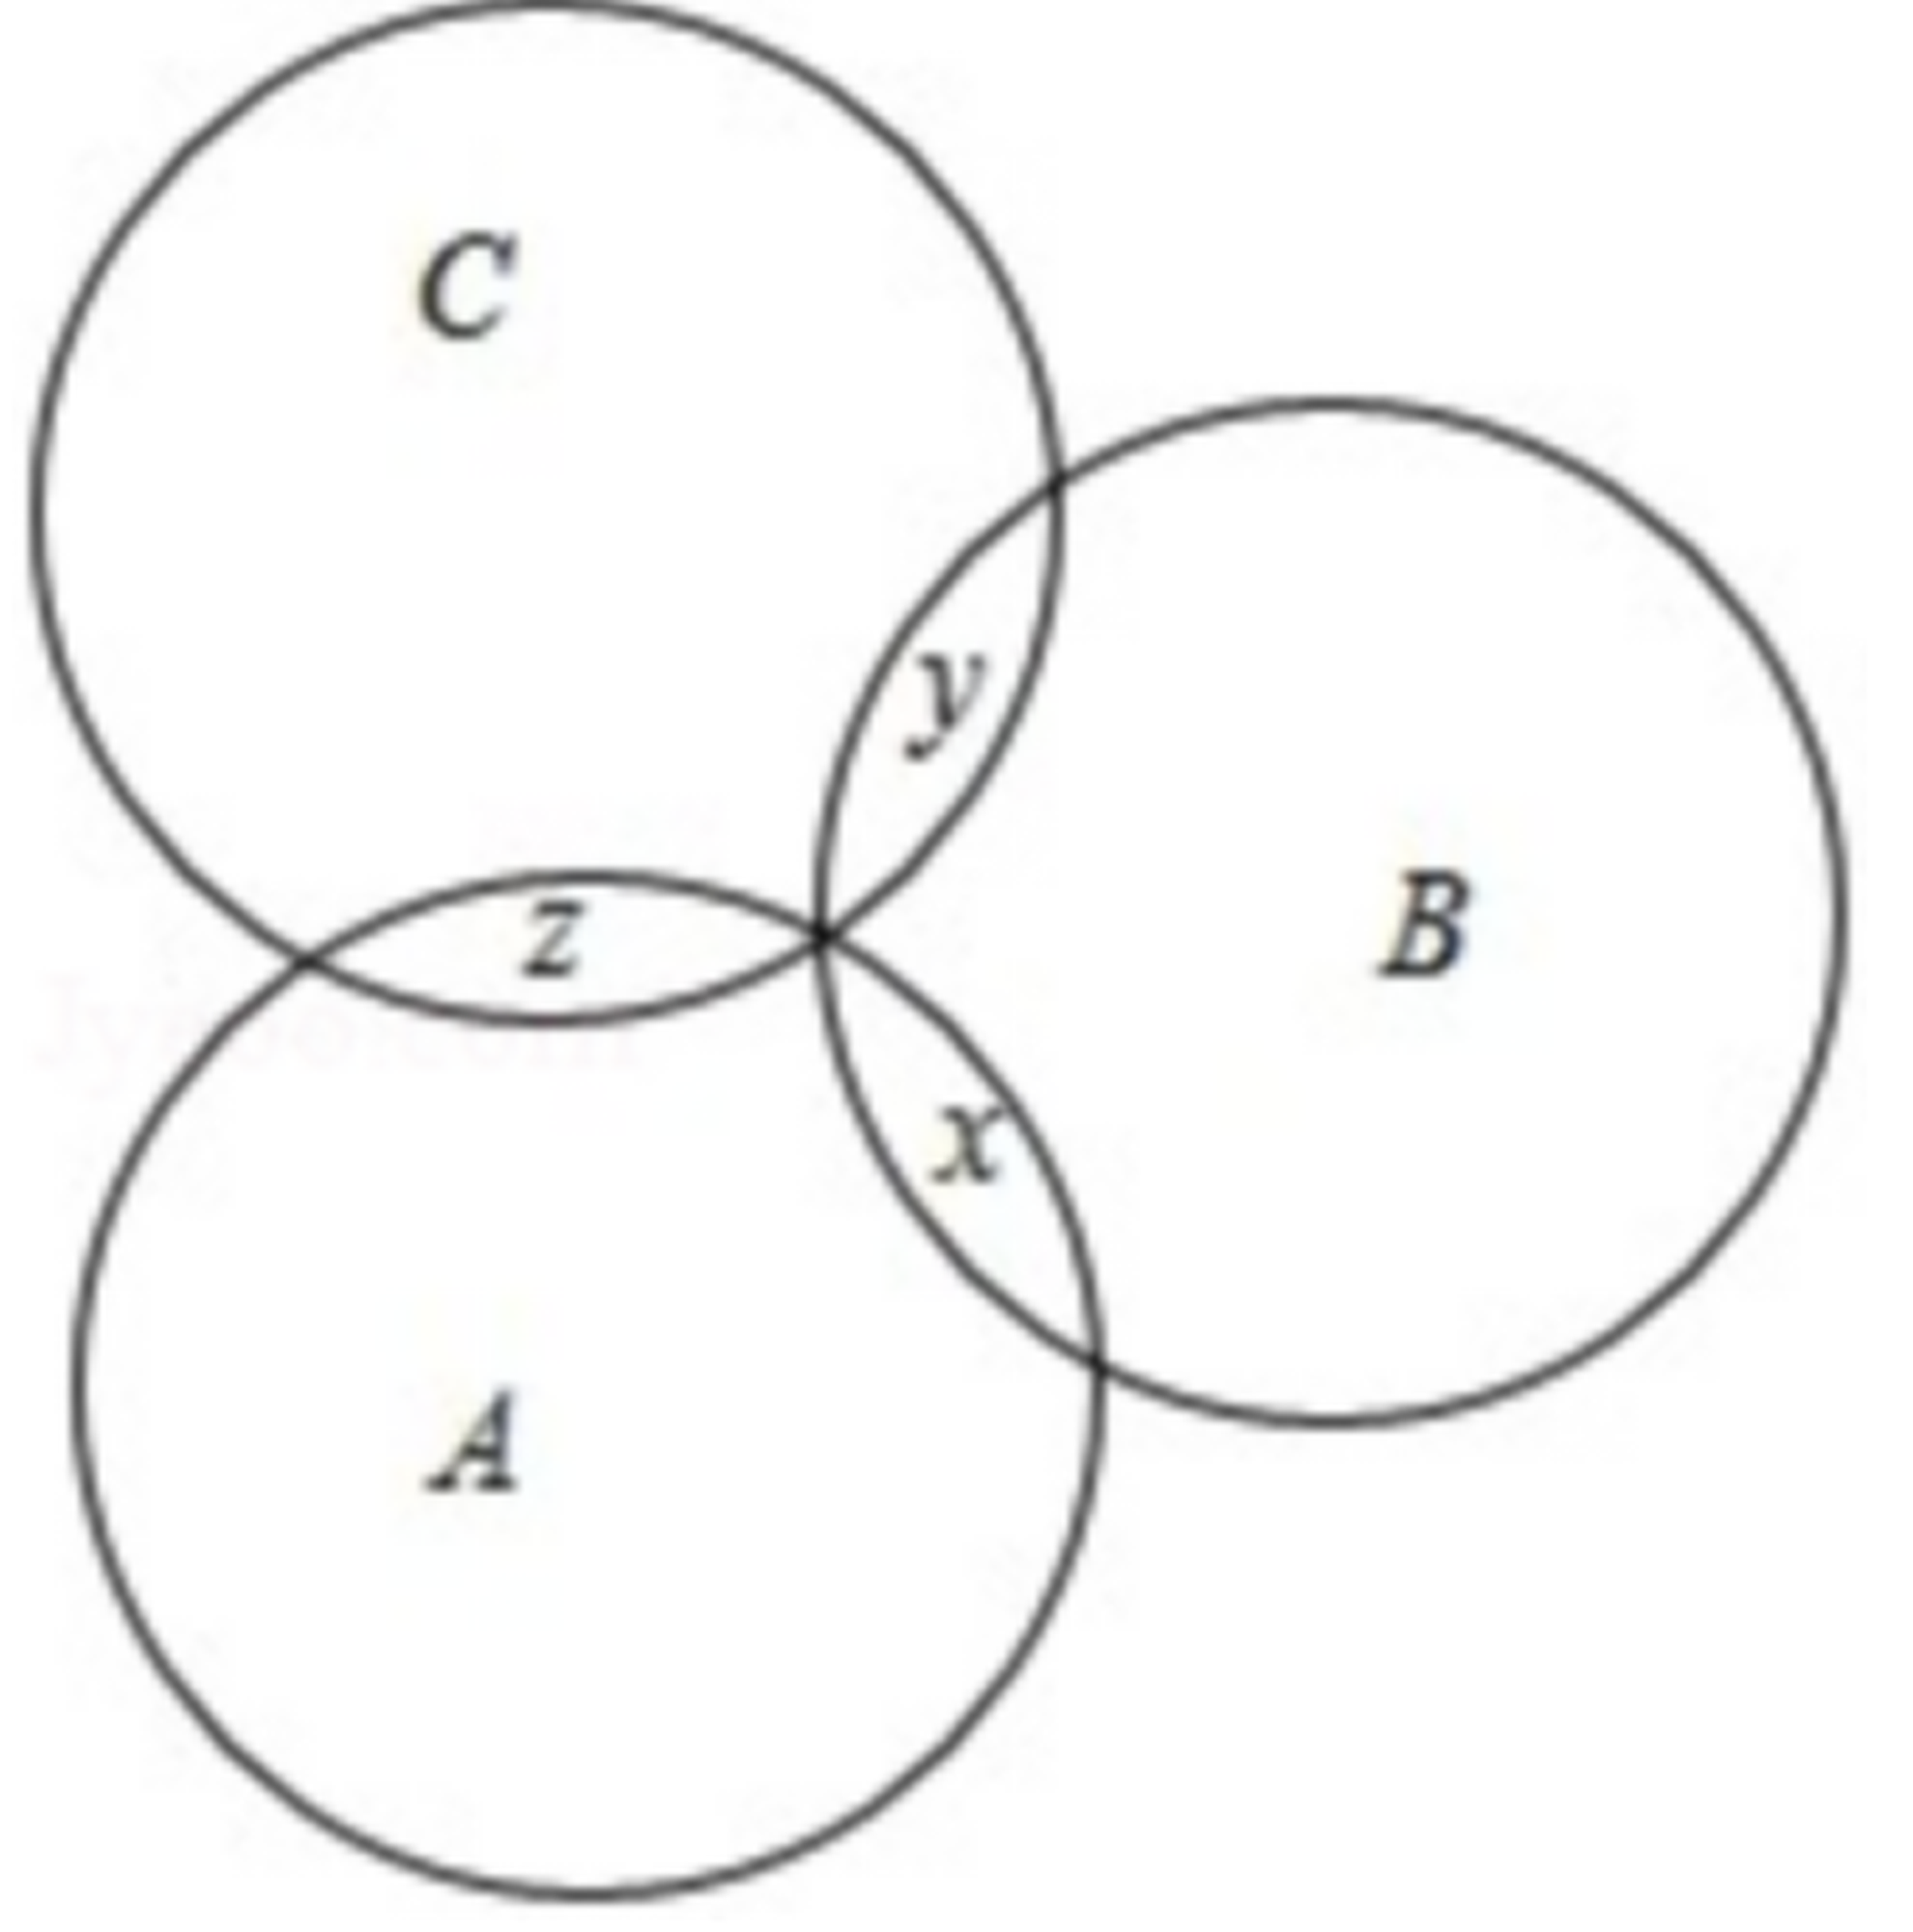
\includegraphics[width=0.30\textwidth]{figures/venn_ABC_x_y_z_h39.png}
\end{center}
\step{因为 $|A\cap B|=|B\cap C|=|C\cap A|=1$，且 $x$、$y$、$z\in\{1,2,3\}$，}
\step{所以集合 $A=\{x,z\}$，$B=\{x,y\}$，$C=\{z,y\}$，}
\step{若 $x=1$，$y=2$，$z=3$，则 $A=\{1,3\}$，$B=\{1,3\}$，$C=\{2,3\}$，}
\step{将 $1$，$2$，$3$ 进行全排列，有 $P_3^3=3\times2=6$ 个.}
\solend

\fi

\item 已知集合 $T=\{1,2,\cdots,2025\}$，对于 $T$ 的每一个非空子集的所有元素，计算它们乘积的倒数，
则所有这样倒数的和为 \blankline[4.4em].

\ans{$2025$}

\ifanswer
\solbegin
\step{集合 $T=\{1,2,\cdots,2025\}$ 的非空子集的个数为 $2^{2025}-1$，}
\step{这些子集中，每个元素的乘积分别为}
\step{$1,2,3,\cdots,2025,1\times2,1\times3,\cdots,1\times2025,\cdots,1\times2\times3\times\cdots\times2025$，}
\step{每项都可以看作是从 $1,2,3,\cdots,2025$ 中选择若干项的乘积，}
\step{$1+\dfrac12+\cdots+\dfrac{1}{2025}+\dfrac{1}{1\times2}+\dfrac{1}{1\times3}+\cdots+\dfrac{1}{2024\times2025}
+\cdots+\dfrac{1}{1\times2\times\cdots\times2025}$}
\step{$=(1+1)\left(1+\dfrac12\right)\cdots\left(1+\dfrac{1}{2025}\right)-1
=2\times\dfrac32\times\dfrac43\times\cdots\times\dfrac{2026}{2025}-1=2025$.}
\solend

\fi

% 第 24 题是压轴题，题干较长；试卷版在它之前量一次页高，尽量不与前文分家（照全稿成例）。
\ansneed{5cm}
% 注：原卷【解析】①③ 两步把 $f(x)$ 印作 $f[x[x]]$，显系笔误，照录未改，见文件头「笔误/存疑」⑦。
\item 若 $X$ 是一个集合，$T$ 是一个以 $X$ 的某些子集为元素的集合，且满足：①$X$ 属于 $T$，
$\varnothing$ 属于 $T$；②$T$ 中任意多个元素的并集属于 $T$；③$T$ 中任意多个元素的交集属于 $T$.
则称 $T$ 是集合 $X$ 上的一个拓扑. 已知函数 $f(x)=[x[x]]$，其中 $[x]$ 表示不大于 $x$ 的最大整数，
当 $x\in(0,n]$，$n\in\N^*$ 时，函数 $f(x)$ 值域为集合 $A_n$，则集合 $A_2$ 上的含有 $4$ 个元素的
拓扑 $T$ 的个数为 \blankline[4.4em].

\ans{$9$}

\ifanswer
\solbegin
\step{由题意，$n=2$，故 $0<x\leqslant2$，}
\step{①当 $0<x<1$ 时，则 $[x]=0$，所以 $f[x[x]]=0$，}
\step{②当 $x=1$ 时，$[x]=1$ 显然 $f(1)=1$，}
\step{③当 $1<x<2$ 时，$[x]=1$，所以 $f[x[x]]=[x]=1$，}
\step{④当 $x=2$ 时，$f(2)=4$，}
\step{所以 $A_2=\{0,1,4\}$，}
\step{因为 $T$ 中含有 $4$ 个元素，其中两个元素 $\varnothing$ 和 $A_2$，}
\step{$A_2=\{0,1,4\}$. 其它两个元素为 $A$、$B$，则
$\begin{cases}A\neq\varnothing\\ A\neq A_2\\ B\neq\varnothing\\ B\neq A_2\\ A\neq B\end{cases}$，}
\step{由对称性，不妨设 $1\leqslant|A|\leqslant|B|\leqslant2$，其中 $|A|$、$|B|$ 表示集合 $A$ 中元素的个数，}
\step{因为 $\begin{cases}A\cap B\in T\\ A\cup B\in T\end{cases}$，又 $|A|\leqslant|B|$，所以 $A\cap B=\varnothing$ 或 $A$，}
\step{若 $A\cap B=\varnothing$，则 $A\cup B$ 只能等于 $A_2$，}
\step{（若 $A\cup B=B$，则 $A\sub B$，则 $A\cap B=A=\varnothing$，矛盾）}
\step{则必有 $\begin{cases}|A|=1\\ |B|=2\end{cases}$，所以 $(A,B)$ 的个数 $\Leftrightarrow$ $A$ 的个数 $=3$ 种，}
\step{即 $\begin{cases}A=\{0\}\\ B=\{1,4\}\end{cases}$ 或 $\begin{cases}A=\{1\}\\ B=\{0,4\}\end{cases}$
或 $\begin{cases}A=\{4\}\\ B=\{0,1\}\end{cases}$；}
\step{若 $A\cap B=A\Leftrightarrow A\sub B$ 此时满足 $A\cup B=B$，}
\step{因为 $A\neq B$ 且 $1\leqslant|A|$ 且 $|B|\leqslant2$，所以 $\begin{cases}|A|=1\\ |B|=2\end{cases}$，}
\step{所以 $B$ 的选择共有 $C_3^2=3$ 种，则 $A$ 的个数有 $C_2^1$ 种，}
\step{所以 $(A,B)$ 的个数 $=2\times3=6$ 种.}
% 这六组「$A$／$B$」按原卷排作两行（前五个一行、第六个另起一行）；因五组并排时
% amsmath 的 cases 会为每组的第二列各留一枚 \quad，本行改排 \left\{\begin{matrix}…\end{matrix}\right.
% 以省下这枚 \quad（照 README「说明」记的高一07 成例），字形与 cases 相同。
\step{（这 $6$ 种是 $\left\{\begin{matrix}A=\{0\}\\ B=\{0,1\}\end{matrix}\right.$、
$\left\{\begin{matrix}A=\{1\}\\ B=\{0,1\}\end{matrix}\right.$、
$\left\{\begin{matrix}A=\{0\}\\ B=\{0,4\}\end{matrix}\right.$、
$\left\{\begin{matrix}A=\{4\}\\ B=\{0,4\}\end{matrix}\right.$、
$\left\{\begin{matrix}A=\{1\}\\ B=\{1,4\}\end{matrix}\right.$、}
\step{$\left\{\begin{matrix}A=\{4\}\\ B=\{1,4\}\end{matrix}\right.$）.}
\step{综上，$T$ 的个数为 $9$ 个.}
\solend

\fi

\end{enumerate}

\end{document}
"
% 紧凑版：xelatex "\def\iscompact{1}% 高一39_大同中学_周末作业4.1.tex
%   —— 高一上数学「2026-2027 年大同中学高一上周末作业 4.1」（试卷版/答案版）
% 试卷版：xelatex 高一39_大同中学_周末作业4.1.tex
% 答案版：xelatex "\def\isanswer{1}% 高一39_大同中学_周末作业4.1.tex
%   —— 高一上数学「2026-2027 年大同中学高一上周末作业 4.1」（试卷版/答案版）
% 试卷版：xelatex 高一39_大同中学_周末作业4.1.tex
% 答案版：xelatex "\def\isanswer{1}\input{高一39_大同中学_周末作业4.1.tex}"
% 紧凑版：xelatex "\def\iscompact{1}\input{高一39_大同中学_周末作业4.1.tex}"
%
% 原始材料是微信公众号图文（公众号「魔都数学加油站」连载「27学年高一 39」，署名「破晓」，
% 2026-09-26 21:29 发布，原文标题「27学年高一39——2026-2027年上海市大同中学高一上周末作业4.1」，
% 原文链接 https://mp.weixin.qq.com/s/HR2hIayXUXNi4zTs3PioiQ ），正文为 11 张 PNG 页。**同一篇里各页分辨率不一致**（2560×3620 与 4762×6735 两档混排：第 1、3、8、10 页为
% 2560×3620，第 2、4、5、6、7、9、11 页为 4762×6735）。原文本身就是一份**讲评版**——除第 15 题
% 外各题题下直接印【解析】（无单独的【答案】行），第 15 题的答案「D」直接印在题干末尾的括号内。
% 试题文字、答案与解析均照原卷录入，未改内容。卷面的粉色斜水印「魔都数学加油站」属水印，未录入。
%
% 卷首标题：原卷页首印作「2026-2027 年大同中学高一上周末作业 4.1」（**卷面标题行即带校名**，
% 年份区间按全稿惯例排 en dash，前缀照原卷保留「年」）。
%
% 篇幅与题号：卷面自「一、填空题」的**第 3 题**起编，终于「附加题」的**第 24 题**，共 22 题
% （填空 3—12、选择 13—16、解答 17—20、附加题 21—24）。第 1、2 题未在该文中发布——这是该
% 公众号连载讲评版的通例（高一02—高一09 等均自第 3 题起编，README「说明」已记），**不是截断**，
% 故本稿题号亦自 3 起。它与 高一40（大同中学 周末作业4.2）同属「周末作业 4」系列但**各自独立起编**
% （4.2 自第 3 题起、终于第 19 题），不是同一份试卷的两半。
%
% 与原卷的排版差异（均已在 README「说明」中交代）：
%   ① 原文自**第 3 题**起（第 1、2 题未在该文中发布），故本稿题号亦自 3 起，填空题以
%      \setcounter{enumi}{2} 起编；选择、解答、附加题三节各按上一节末号另设 \setcounter
%      （选择题 \setcounter{enumi}{12}、解答题 \setcounter{enumi}{16}、附加题 \setcounter{enumi}{20}）；
%   ② 原卷本就印有「一、填空题」「二、选择题」「三、解答题」三节标题，末节印作「附加题」
%      （**不带「四、」**，且题号 21—24 续前编、不另起），本稿照原卷分节，只把标题改排成全稿
%      统一的「大节标题」样式；
%   ③ 原卷是「讲评版」：除第 15 题外，各题题下均印【解析】（**全卷无一条独立的【答案】行**）；
%      第 15 题无解析，答案「D」直接印在题干末尾的括号内。本稿统一改为试卷版隐去、答案版以
%      \ans{}／\ifanswer 块给出，两版彻底分离；原卷写在【解析】末句的结果，本稿照 高一38
%      （同校同系列、同为讲评版）的成例另提为 \ans{}；
%   ④ 数集记号原卷两套并用：实数集作斜体的 $R$（第 7、11、14、17、18、19 题），整数集作斜体
%      $Z$（第 10 题），自然数集作斜体 $N$ 及 $N^*$（第 16、20、21、24 题），本稿按全稿惯例
%      统一写作 $\R$、$\Z$、$\N$、$\N^*$；
%   ⑤ 补集符号原卷两套并用：第 7 题作前缀式的 $C_U$（且题干称全集为 $I$，见「笔误/存疑」①），
%      第 14、15、18 题作上横线（$\overline{H}$、$\overline{A}$、$\overline{B}$），本稿照录、不归一
%      （前缀式写作 $\complement_U$，与 高一c／高一10 的成例一致）；
%   ⑥ 包含符号原卷两套并用：第 3 题作**无下划线**的 $\subset$，第 15、18、20、24 题作**带下划线**
%      的 $\sub$，本稿照录、不归一；
%   ⑦ 原卷填空的横线约两个字宽，本稿按全稿惯例统一排 \blankline[4.4em]；
%   ⑧ 第 7、11、22 题各有插图，取原卷截图、4× LANCZOS 放大（figures/venn_N_cap_CI_M_h39.png、
%      figures/plane_grid_4squares_h39.png、figures/venn_ABC_x_y_z_h39.png）；第 7 题的 Venn 属
%      **题干**（试卷版、答案版都出），第 11、22 题的图在【解析】内（仅答案版出）。第 7 题图
%      左下、第 11 题图的上／左／右边缘带进极淡的原卷粉色水印残影——照全稿「插图直接取自
%      原卷截图、不用 TikZ 重绘、不修图」的体例保留（再裁会切到坐标轴与 $x$、$y$、$O$ 标注）；
%   ⑨ 原卷并列的字母、数字（「$x_1,x_2$」「$a,b$」「$1,2,3,\cdots,11$」）多作半角逗号或不加标点，
%      本稿按全稿惯例改排顿号（$x_1$、$x_2$）或把数列并入行内公式；半角括号、逗号一律排全角，
%      数学式内部的标点照原样；
%   ⑩ 原卷未印副标题，本稿按**本卷实际内容**补出副标题「集合与常用逻辑用语」（依据见下条）。
%
% 副标题（\examtitlest 第二个参数）：本卷卷面未印副标题，由本稿补出，取值按 2026-09-26 起的
%   新口径「只用本卷实际内容的模块名」定为「集合与常用逻辑用语」。依据：全卷 22 题（第 3—24 题）中，
%   第 3、5、7、8、10、11、14、15、16、17、18、19、20、21、22、23、24 题共 17 题是集合的运算与
%   关系、子集／真子集、补集、集合新定义（「全食／偏食」、最小相交、拓扑、特征数）与集合计数，
%   以及命题与常用逻辑用语（第 3 题充要条件、第 5 题存在量词命题、第 17 题命题真假）；其余两题
%   第 4、6 考一元二次方程的根（韦达定理）与方程恒等，第 9、12、13 题是不等式（一元二次不等式组
%   的整数解、一元二次不等式解集、不等式的性质）——不等式合计 3/22，**不足全卷三分之一**，
%   故不并标「不等式」。
%
% 原卷笔误/存疑（均照抄原卷、未改，见源码中该处上方注释）：
%   ① 第 7 题题干称「全集 $I=R$」，而【解析】两处把补集写作 $C_U M$（下标作 $U$），前后记号不一；
%      本稿照录，未改；
%   ② 第 4 题【解析】两处把判别式印作 $\triangle=[2(m-1)^2-16m^2]$（方括号内首项漏了平方，
%      正确应作 $[2(m-1)]^2-16m^2$）；按其所判「$m=\frac12$ 时 $<0$、$m=-\frac12$ 时 $>0$」反推，
%      $[2(m-1)]^2-16m^2$ 在 $m=\frac12$ 时为 $-3<0$、在 $m=-\frac12$ 时为 $5>0$，与结论一致；
%      本稿照录；
%   ③ 第 9 题【解析】把方程组第二式印作 $1-2<-k\leqslant3$，按其结论 $-3\leqslant k<2$ 反推，
%      疑当作 $-2<-k\leqslant3$（原卷多一个「$1$」）；本稿照录；
%   ④ 第 17 题【解析】首句「由数 $y=-x^2+ax-1=-x+3$」中的「由数」显系「由」或「由函数」之误；
%      且末段「若 $p$ 真 $q$ 假…得 $a\in R$」「若 $p$ 假 $q$ 真…此时 $a$ 无解」与结论「$a$ 的取值范围
%      是 $R$」自相矛盾（按 $p:a\leqslant-5$、$q:a>-6$，$p$ 真 $q$ 假应为 $a\leqslant-6$，$p$ 假 $q$ 真
%      应为 $a>-5$，合起来是 $a\leqslant-6$ 或 $a>-5$，并非 $R$）；本稿一律照录，未按正确解法改写；
%   ⑤ 第 18 题【解析】(2) 把 $B=\{x\mid x^2+a\leqslant0\}$（$a<0$）印作右端开的
%      $\{x\mid-\sqrt{-a}\leqslant x<\sqrt{-a}\}$（应为闭的「$\leqslant$」）；按其所判
%      $\sqrt{-a}<\frac12$ 反推，不影响结论；本稿照录；
%   ⑥ 第 22 题【解析】在 $x=1$、$y=2$、$z=3$ 时把 $B=\{x,y\}$ 印作 $\{1,3\}$（应为 $\{1,2\}$），
%      与本行前面「$B=\{x,y\}$」不合；本稿照录；
%   ⑦ 第 24 题【解析】①③ 两步把 $f(x)$ 印作 $f[x[x]]$，显系笔误；本稿照录。
%   ⑧ 第 8 题【解析】「即方程 $x^2+ax+b=x$，$x^2+(a-1)x+b=0$ **由**两个相等的实数根为 $4$」——
%      「由」当为「有」（「设…是…有」的杂糅）；本稿照录；
%   ⑨ 第 10 题：题设 $a\oplus b=b(a^2+b^2+1)$，而集合定义里含 $\dfrac{a\oplus b}{2b}$；$-2<a<b<2$、
%      $a$、$b\in\Z$ 时 $(a,b)=(-1,0)$ 也合条件、却使分母 $2b=0$，原卷解析仍代入该组并约去
%      $b$ 得 $x=1$（答案集恰好不变）；本稿照录；
%   ⑩ 第 15 题选项列里 ② 与 ③ 之间**漏排分隔号**（原卷作「② $\overline{A}\cap B=\varnothing$③
%      $\overline{A}\sub\overline{B}$；」——①、③ 后都有「；」，② 后没有）；本稿照录；
%   ⑪ 第 20(2) 把 $\{1,2,\cdots,20\}$ 分成的 11 个集合里，$\{8,11\}$ 与 $\{9,12\}$ 之间误用
%      **句号**「.」（同行其余处皆逗号）；本稿照录；
%   ⑫ 第 20(3)① 推理不严：原卷写「选 5 则不选 1、9；选 6 则不选 2、10；选 7 则不选 3、11；
%      则只剩 4、8」——但 4 与 8 相差 $4$、不能同选，该情形实际最多只能取 $4$ 个；末句结论
%      「不超过 $5$ 个」仍成立；本稿照录；
%   ⑬ 第 16 题【解析】两种下标并存：「所以在 $A_i$ 的特征数构成中」原卷作斜体 $A_i$，而
%      「要使 $X_1+X_2+X_3$ 最大（小），则（应）在集合 $A_1$ 中首先放置…」两处原卷作
%      **数字 $1$**（与同句 $X_1$ 的角标同形）；本稿照录、未归一。
%
% 图取原卷截图（依次见各处的 \includegraphics 前的注释），4× LANCZOS 放大。
\documentclass[a4paper,11pt]{article}
\usepackage{common}

\begin{document}

\examtitlest[3]{2026--2027 年大同中学高一上周末作业 4.1}{集合与常用逻辑用语}

\bigsec{一、填空题}

\begin{enumerate}
\setcounter{enumi}{2}

\item “$x\geqslant a$”是“$0<x<2$”的必要非充分条件，则实数 $a$ 的取值范围是 \blankline[4.4em].

\ans{$(-\infty,0]$}

\ifanswer
\solbegin
\step{因为 $x\geqslant a$ 是 $0<x<2$ 的必要非充分条件，所以 $(0,2)\subset[a,+\infty)$，所以 $a\leqslant0$，}
\step{则实数 $a$ 的取值范围是 $(-\infty,0]$.}
\solend

\fi

% 注：原卷$[2(m-1)^2-16m^2]$ 首项漏了平方（应为 $[2(m-1)]^2-16m^2$），照录未改，见文件头「笔误/存疑」②。
\item 若关于 $x$ 的方程 $x^2+2(m-1)x+4m^2=0$ 有两个实数根，且这两根互为倒数，则 $m=$ \blankline[4.4em].

\ans{$-\dfrac12$}

\ifanswer
\solbegin
\step{设 $x_1$、$x_2$ 是方程 $x^2+2(m-1)x+4m^2=0$ 有两个实数根，}
\step{则 $x_1x_2=4m^2=1$，解得 $m=\dfrac12$ 或 $m=-\dfrac12$，}
\step{又当 $m=\dfrac12$ 时，$\triangle=[2(m-1)^2-16m^2]<0$，舍去，}
\step{当 $m=-\dfrac12$ 时，$\triangle=[2(m-1)^2-16m^2]>0$，故 $m=-\dfrac12$.}
\solend

\fi

\item 已知命题：“存在 $x\in[1,2]$，使 $x^2+2x+a\geqslant0$”为真命题，则 $a$ 的取值范围是 \blankline[4.4em].

\ans{$a\geqslant-8$}

\ifanswer
\solbegin
\step{若存在 $x\in[1,2]$，使 $x^2+2x+a\geqslant0$，}
\step{则等价为存在 $x\in[1,2]$，使 $x^2+2x\geqslant-a$，}
\step{当存在 $x\in[1,2]$ 时，设 $y=x^2+2x=(x+1)^2-1$，则 $3\leqslant y\leqslant8$，}
\step{所以要使 $x^2+2x\geqslant-a$，则 $8\geqslant-a$，即 $a\geqslant-8$.}
\solend

\fi

\item 已知方程 $a(3x+2)+b(2x-3)=8x+3$ 有无穷多个解，则 $a:b=$ \blankline[4.4em].

\ans{$30:7$}

\ifanswer
\solbegin
\step{$a(3x+2)+b(2x-3)=(3a+2b)x+2a-3b=8x+3$ 有无穷多个解，}
\step{所以 $\begin{cases}3a+2b=8\\ 2a-3b=3\end{cases}$，解得 $a=\dfrac{30}{13}$，$b=\dfrac{7}{13}$，所以 $a:b=30:7$.}
\solend

\fi

% 注：原卷题干称「全集 $I=R$」，而【解析】两处把补集写作 $C_U M$（下标作 $U$），前后记号不一；
%     照录未改，见文件头「笔误/存疑」①。
\item 已知集合 $M=\{x\mid y=\sqrt{3-x^2}\}$，$N=\{x\mid-3\leqslant x\leqslant1\}$，全集 $I=\R$，
则图中阴影部分表示的集合为 \blankline[4.4em].

% 图取原卷截图（01.png，2560×3620）右栏，4× LANCZOS 放大。
\begin{center}
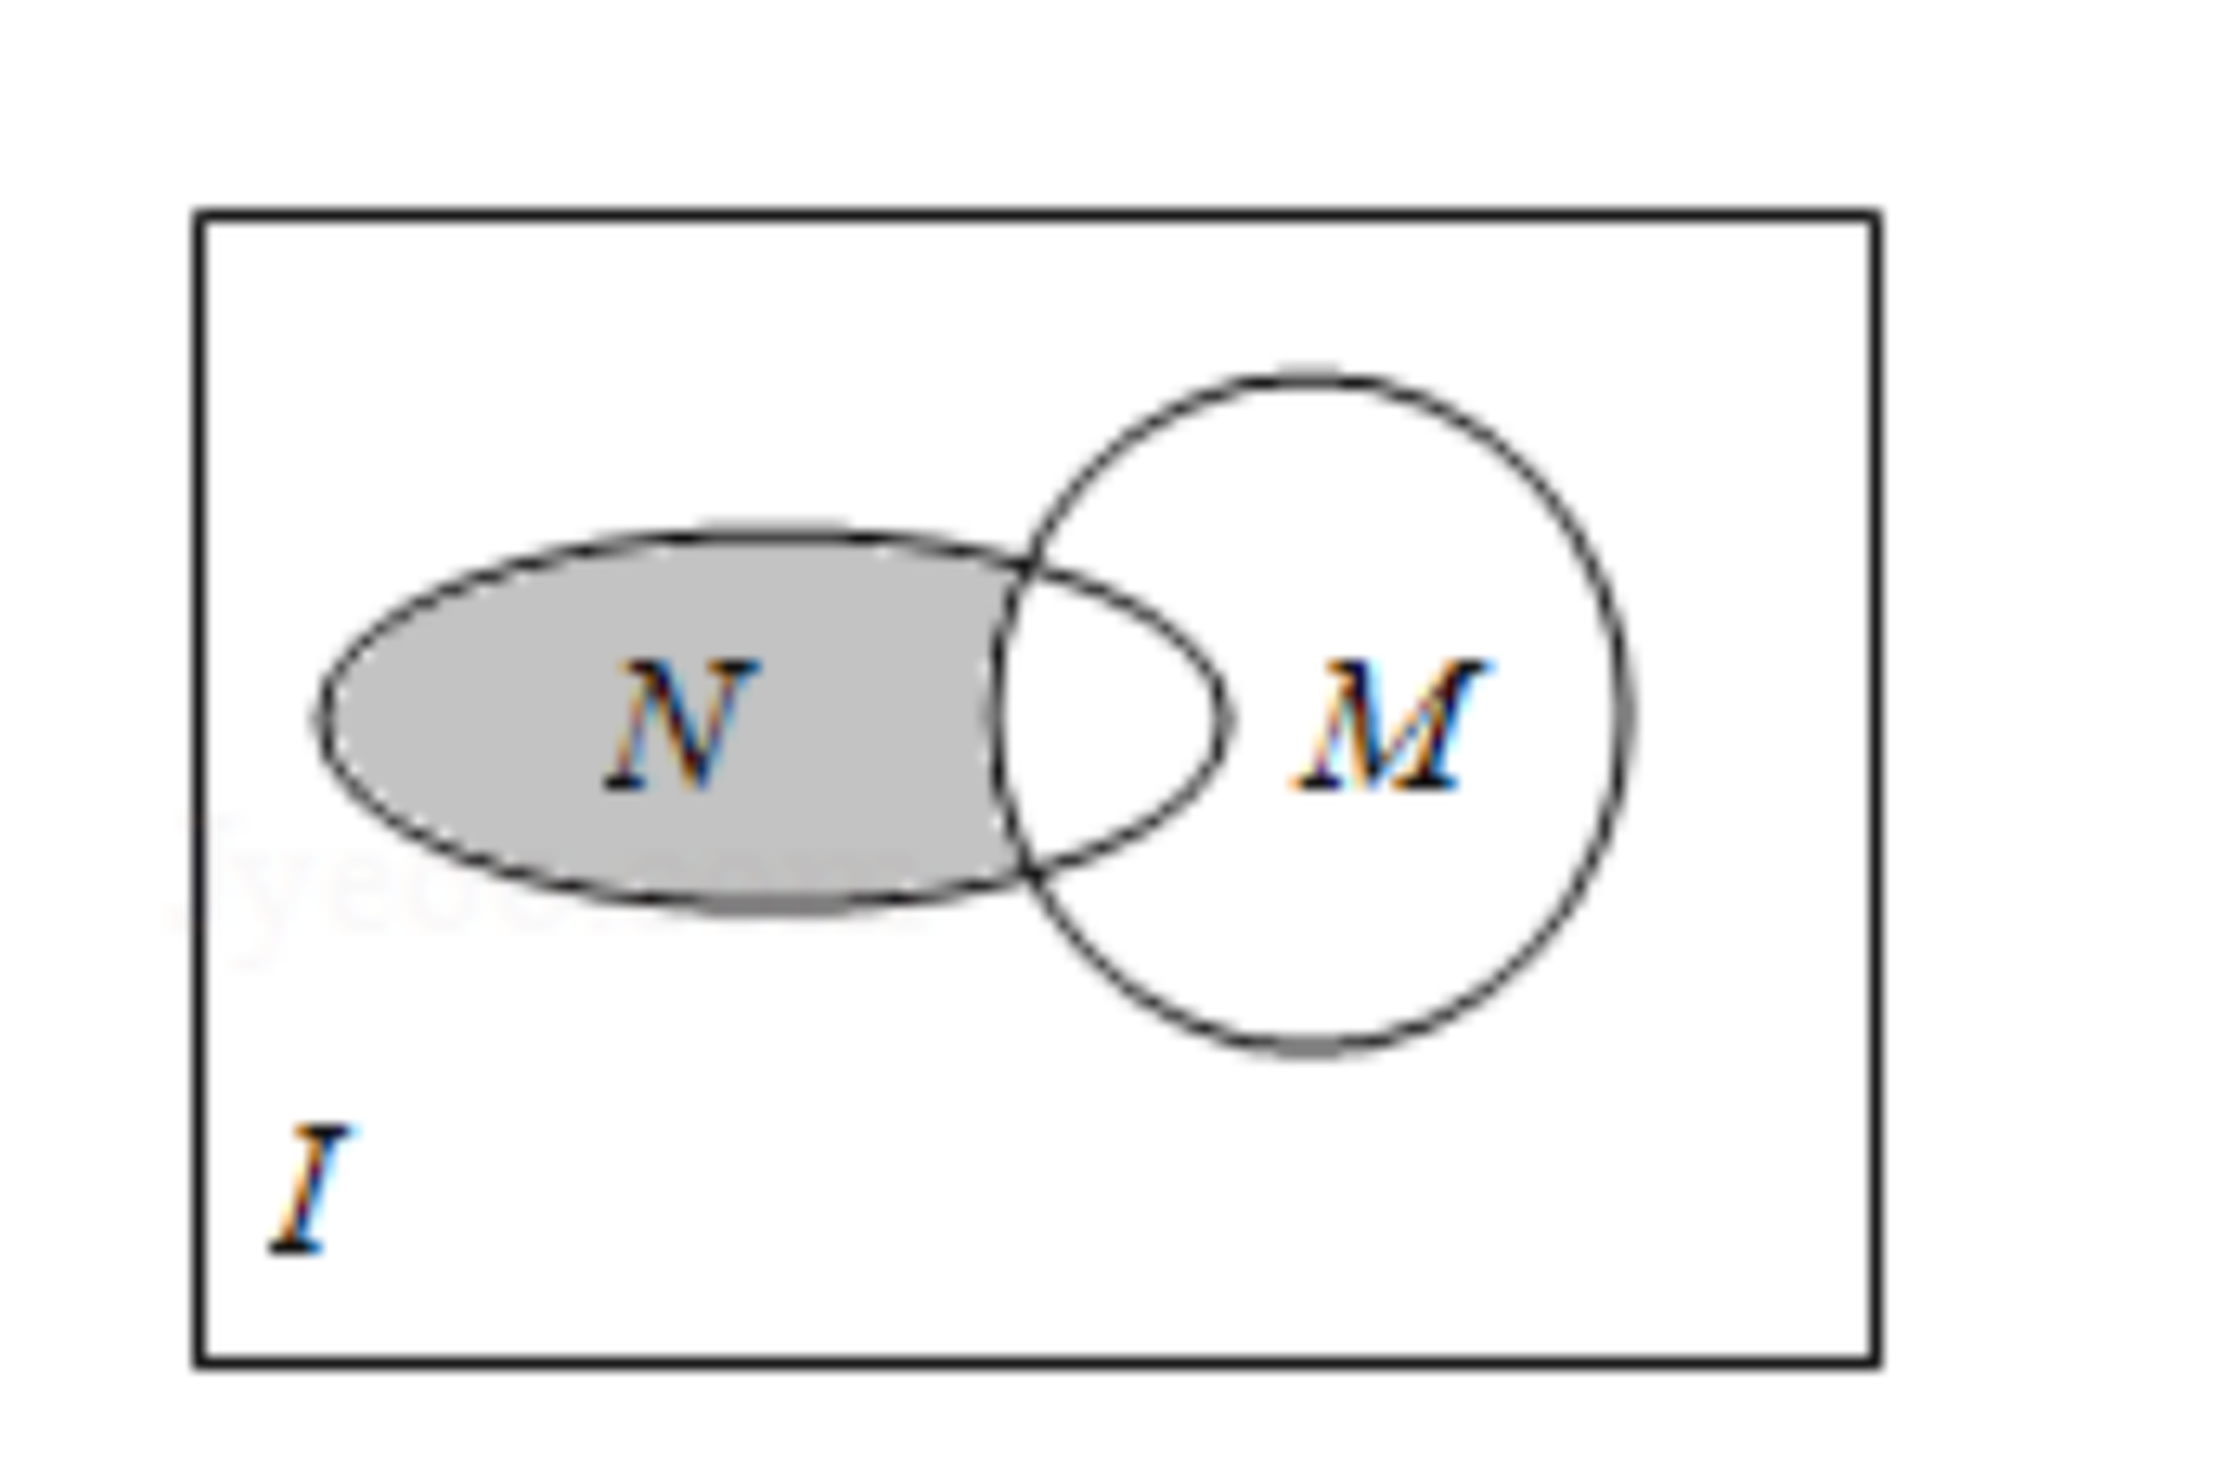
\includegraphics[width=0.30\textwidth]{figures/venn_N_cap_CI_M_h39.png}
\end{center}

\ans{$[-3,-\sqrt3)$}

\ifanswer
\solbegin
\step{阴影部分用集合表示为 $N\cap(\complement_UM)$.}
\step{则 $M=\{x\mid y=\sqrt{3-x^2}\}=\{x\mid3-x^2\geqslant0\}=\{x\mid-\sqrt3\leqslant x\leqslant\sqrt3\}$，}
\step{则 $\complement_UM=\{x\mid x>\sqrt3\text{ 或 }x<-\sqrt3\}$，$N=\{x\mid|x+1|\leqslant2\}=\{x\mid-3\leqslant x\leqslant1\}$，}
\step{则 $N\cap(\complement_UM)=\{x\mid-3\leqslant x<-\sqrt3\}$.}
\solend

\fi

\item 已知 $f(x)=x^2+ax+b$，集合 $\{x\mid f(x)=x\}=\{4\}$，将集合 $M=\{x\mid f(x)=4\}$ 用列举法表示 \blankline[4.4em].

\ans{$\{3,4\}$}

\ifanswer
\solbegin
\step{已知 $f(x)=x^2+ax+b$，集合 $\{x\mid f(x)=x\}=\{4\}$，}
% 注：原卷本行作「…$x^2+(a-1)x+b=0$ **由**两个相等的实数根为 $4$」——「由」当为「有」
%     （「设…是…有」的杂糅）；本稿照录未改，见文件头「原卷笔误/存疑」⑧。
\step{即方程 $x^2+ax+b=x$，$x^2+(a-1)x+b=0$ 由两个相等的实数根为 $4$，}
\step{所以 $\triangle=(a-1)^2-4b=0$，即 $x^2+(a-1)x+b=(x-4)^2$，所以 $b=16$，$a=-7$，}
\step{所以 $f(x)=x^2+ax+b=x^2-7x+16$，所以集合 $M=\{x\mid f(x)=4\}$，}
\step{即 $x^2-7x+16=4$，$x^2-7x+12=0$，故 $M=\{x\mid f(x)=4\}=\{3,4\}$.}
\solend

\fi

% 注：原卷方程组第二式印作 $1-2<-k\leqslant3$，按其结论 $-3\leqslant k<2$ 反推疑当作 $-2<-k\leqslant3$，
%     照录未改，见文件头「笔误/存疑」③。
\item 关于 $x$ 的不等式组 $\begin{cases}x^2-x-2>0\\ 2x^2+(2k+5)x+5k<0\end{cases}$ 的整数解的集合为 $\{-2\}$，
则实数 $k$ 的取值范围 \blankline[4.4em].

\ans{$-3\leqslant k<2$}

\ifanswer
\solbegin
\step{原不等式组即 $\begin{cases}(x-2)(x+1)>0\\ (x+k)(2x+5)<0\end{cases}$，整数解的集合为 $A$，若 $A=\{-2\}$，}
\step{则 $(-2+k)(2\times(-2)+5)<0$，所以 $k<2$，且有 $\begin{cases}-k>-\dfrac52\\ 1-2<-k\leqslant3\end{cases}$，}
\step{解得 $-3\leqslant k<2$.}
\solend

\fi

\item 规定 $\oplus$ 与 $\otimes$ 是两个运算符号，其运算法则如下，对任意实数 $a$、$b$ 有：$a\otimes b=ab$，
$a\oplus b=b(a^2+b^2+1)$. 若 $-2<a<b<2$ 且 $a$、$b\in\Z$，
$A=\left\{x\mid x=2(a\otimes b)+\dfrac{a\oplus b}{2b}\right\}$，则用列举法表示集合 $A=$ \blankline[4.4em].

\ans{$\left\{1,-\dfrac12\right\}$}

\ifanswer
\solbegin
\step{$A=\left\{x\mid x=2(a\otimes b)+\dfrac{a\oplus b}{2b}\right\}
=\left\{x\mid x=2ab+\dfrac{b(a^2+b^2+1)}{2b}\right\}$}
\step{$=\left\{x\mid x=2ab+\dfrac12a^2+\dfrac12b^2+\dfrac12\right\}
=\left\{x\mid x=\dfrac12(a+b)^2+ab+\dfrac12\right\}$，}
% 注：题设含 $\dfrac{a\oplus b}{2b}$，而 $-2<a<b<2$、$a$、$b\in\Z$ 时 $(a,b)=(-1,0)$ 也合条件、
%     却使分母 $2b=0$；原卷解析仍代入该组并约去 $b$ 得 $x=1$（答案集恰好不变）。本稿照录，
%     见文件头「原卷笔误/存疑」⑨。
\step{当 $a=-1$，$b=0$ 时，$x=1$；当 $a=-1$，$b=1$ 时，$x=-\dfrac12$；}
\step{当 $a=0$，$b=1$ 时，$x=1$；所以 $A=\left\{1,-\dfrac12\right\}$.}
\solend

\fi

\item 高斯是德国著名的数学家，近代数学奠基者之一，享有“数学王子”的称号，为了纪念数学家高斯，
我们把取整函数 $y=[x]$，$x\in\R$ 称为高斯函数，其中 $[x]$ 表示不超过 $x$ 的最大整数，
如 $[1.1]=1$，$[-1.1]=-2$. 则点集 $P=\{(x,y)\mid[x]^2+[y]^2=1\}$
所表示的平面区域的面积是 \blankline[4.4em].

\ans{$4$}

\ifanswer
\solbegin
\step{$[x]^2+[y]^2=1$ 由 $\begin{cases}[x]=0\\ [y]=-1\end{cases}$ 或 $\begin{cases}[x]=0\\ [y]=1\end{cases}$
或 $\begin{cases}[x]=-1\\ [y]=0\end{cases}$ 或 $\begin{cases}[x]=1\\ [y]=0\end{cases}$ 四个平面区域组成，}
\step{即 $\begin{cases}0\leqslant x<1\\ -1\leqslant y<0\end{cases}$ 或 $\begin{cases}0\leqslant x<1\\ 1\leqslant y<2\end{cases}$
或 $\begin{cases}-1\leqslant x<0\\ 0\leqslant y<1\end{cases}$ 或 $\begin{cases}1\leqslant x<2\\ 0\leqslant y<1\end{cases}$，}
\step{作出平面区域如图所示，平面区域由四个边长为 $1$ 的正方形组成，}
% 图在【解析】内（仅答案版出），取原卷截图（03.png，2560×3620）中部，4× LANCZOS 放大。
\begin{center}
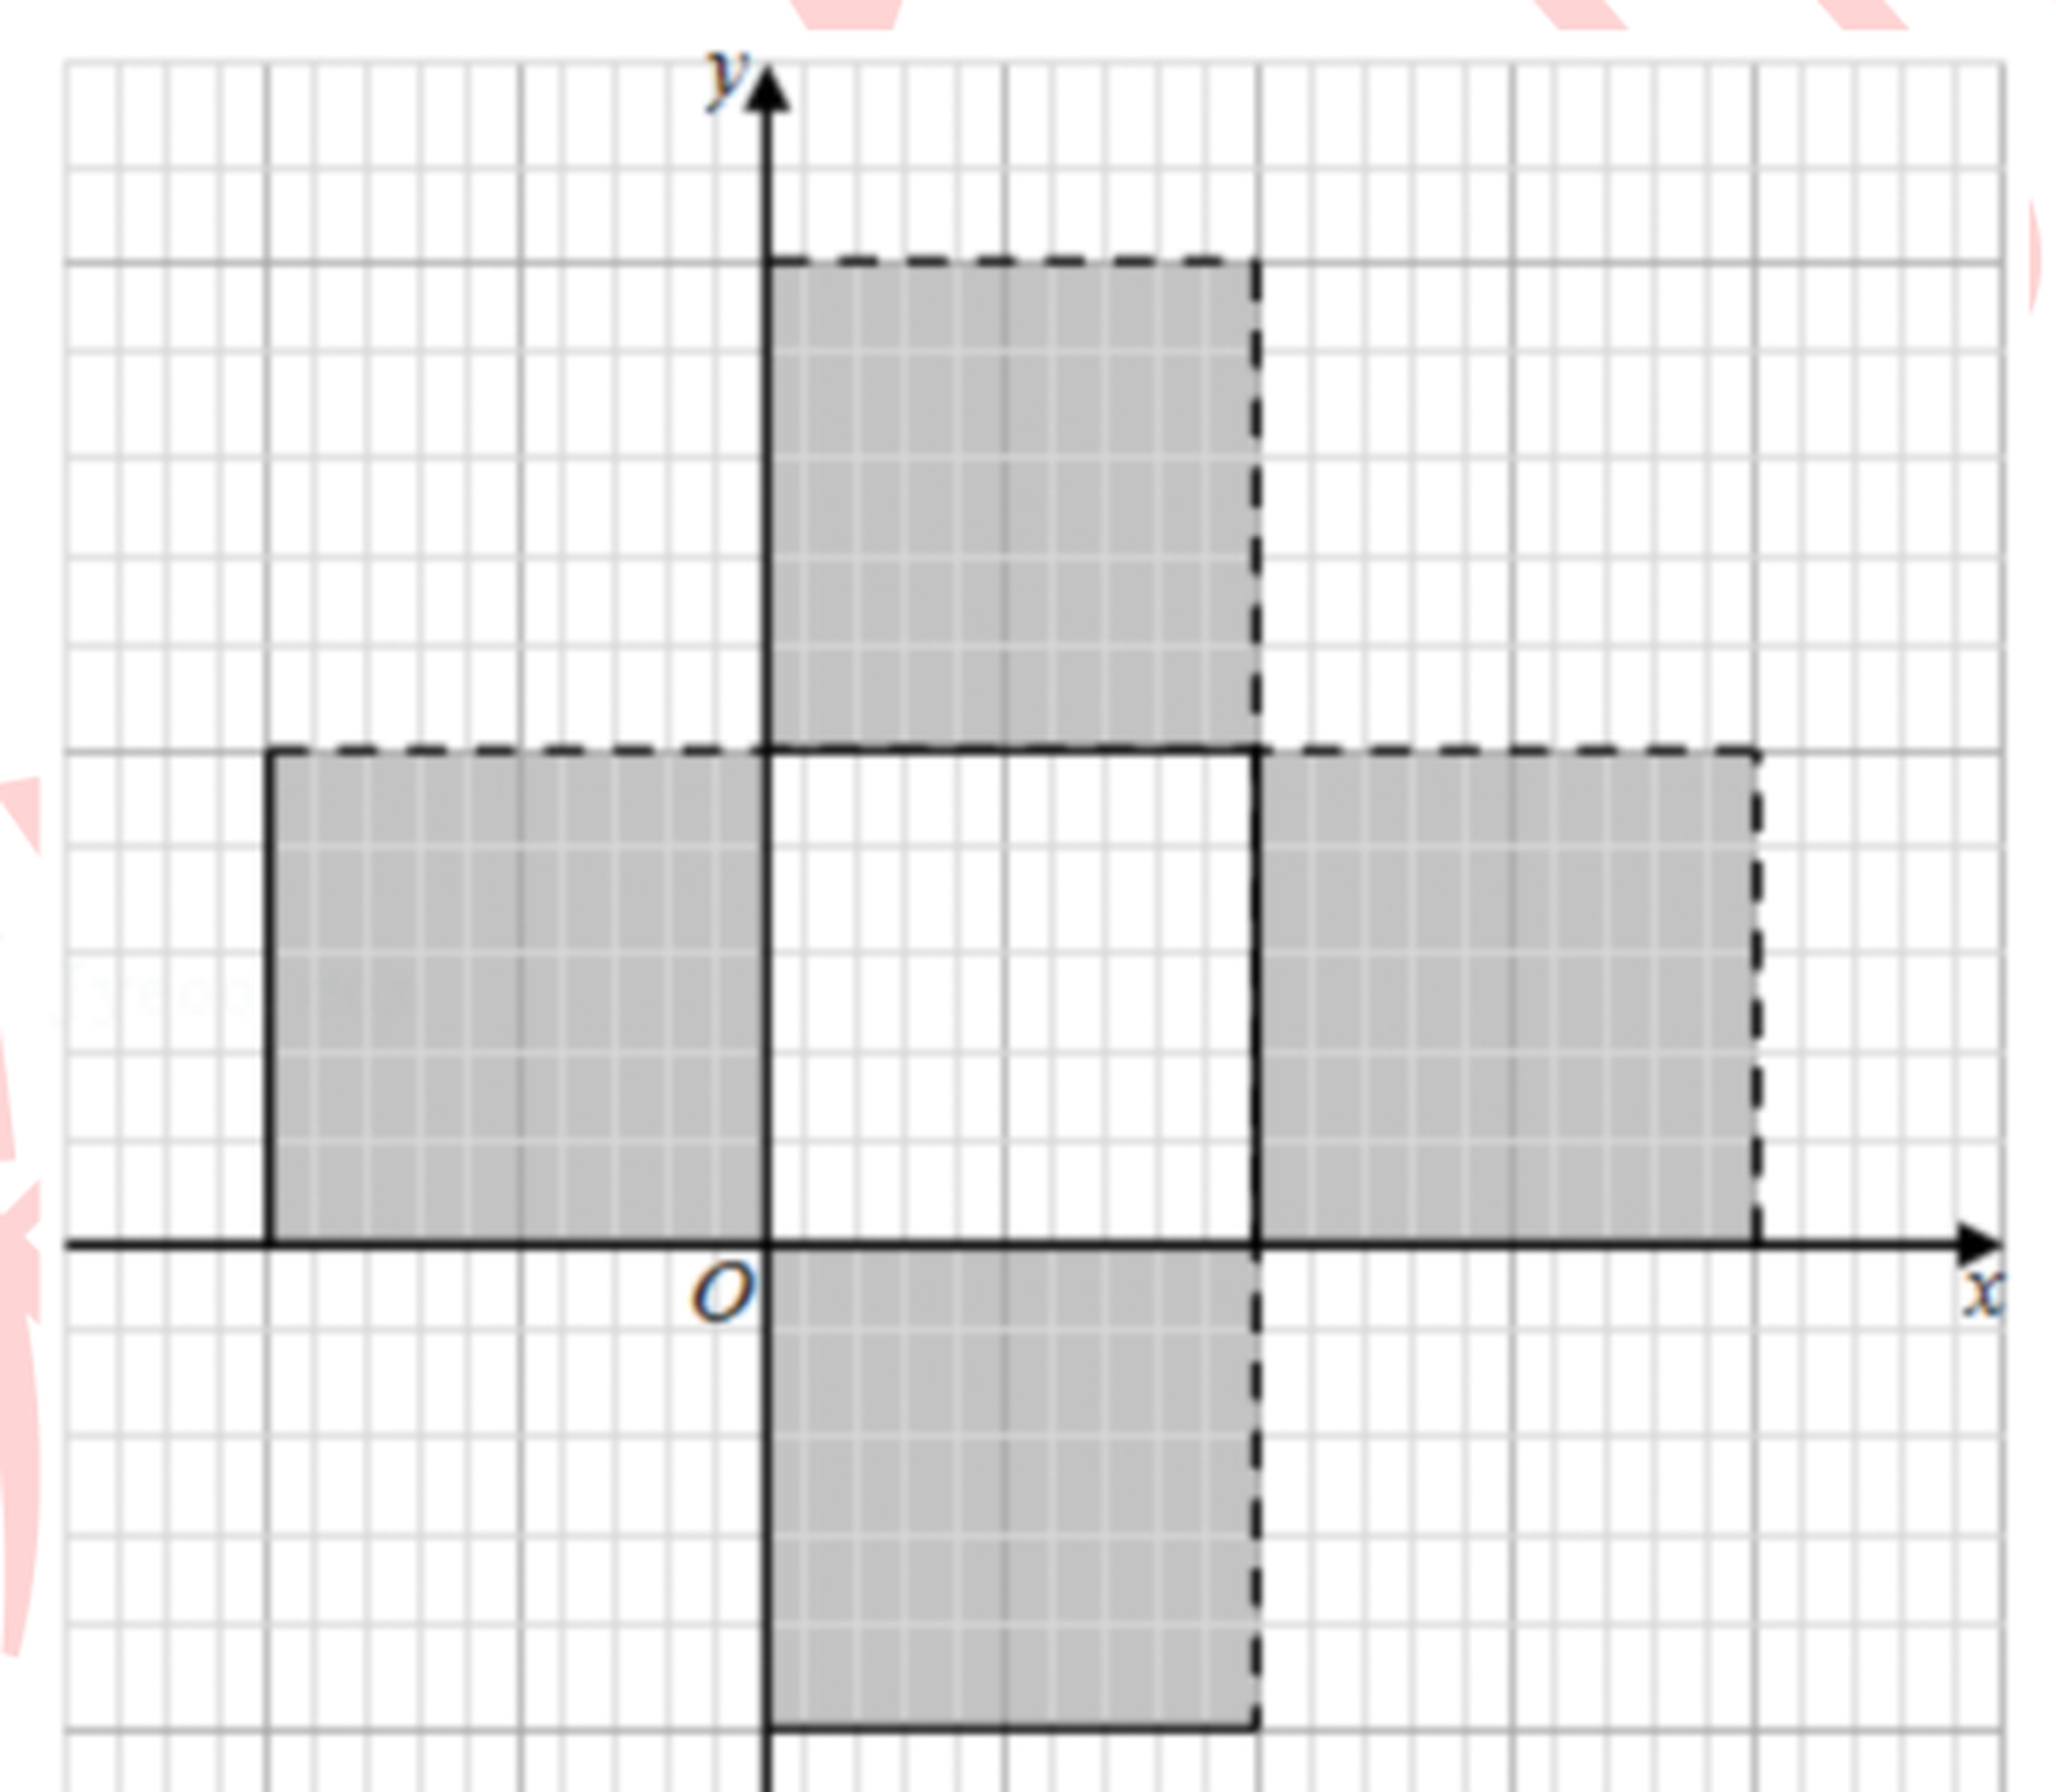
\includegraphics[width=0.38\textwidth]{figures/plane_grid_4squares_h39.png}
\end{center}
\step{总面积为 $1\times4=4$.}
\solend

\fi

\item 关于 $x$ 的不等式 $ax^2+bx+c>0$ 的解集为 $\{x\mid x<\beta\text{ 或 }x>\gamma\}(0<\beta<\gamma)$，
则不等式 $a(x^2+1)+b(x-1)+c>2ax$ 的解集为 \blankline[4.4em].

\ans{$(-\infty,\beta+1)\cup(\gamma+1,+\infty)$}

\ifanswer
\solbegin
\step{由题意得 $\beta$、$\gamma$ 为方程 $ax^2+bx+c=0$ 的两根且 $a>0$，}
\step{则 $\beta+\gamma=-\dfrac ba$，$\beta\gamma=\dfrac ca$，故 $b=-a(\beta+\gamma)$，$c=\beta\gamma a$，}
\step{则不等式可化为 $a(x^2+1)-a(\beta+\gamma)(x-1)+\beta\gamma a>2ax$，}
\step{因为 $a>0$，所以 $x^2+1-(\beta+\gamma)(x-1)+\beta\gamma>2x$，}
\step{即 $x^2-(\beta+\gamma+2)x+(\beta+\gamma+\beta\gamma+1)>0$，所以 $(x-\beta-1)(x-\gamma-1)>0$，}
\step{解得 $x<\beta+1$ 或 $x>\gamma+1$，所以不等式解集为 $(-\infty,\beta+1)\cup(\gamma+1,+\infty)$.}
\solend

\fi

\end{enumerate}

\bigsec{二、选择题}

\begin{enumerate}
\setcounter{enumi}{12}

\item 设 $a<b<0$，则下列不等式中不成立的是\mbox{（\quad）}

\keepwithprev
A. $\dfrac1a>\dfrac1b$\qquad B. $\dfrac{1}{a-b}>\dfrac1a$\qquad C. $|a|>-b$\qquad D. $\sqrt{-a}>\sqrt{-b}$

\ans{$B$}

\ifanswer
\solbegin
\step{令 $a=-2$，$b=-1$，}
\step{A、$-\dfrac12>-1$，正确；B、$-1<-\dfrac12$，故 B 错误；C、$2>1$，正确；}
\step{D、$\sqrt2>1$，正确；故选 B.}
\solend

\fi

\item 设实数集 $\R$ 为全集，集合 $P=\{x\mid f(x)=0\}$，$Q=\{x\mid g(x)=0\}$，$H=\{x\mid h(x)=0\}$，
则方程 $\dfrac{f^2(x)+g^2(x)}{h(x)}=0$ 的解集是\mbox{（\quad）}

\keepwithprev
A. $P\cap Q\cap\overline{H}$\qquad B. $P\cap Q$\qquad C. $P\cap Q\cap H$\qquad D. $P\cap Q\cup H$

\ans{$A$}

\ifanswer
\solbegin
\step{方程 $\dfrac{f^2(x)+g^2(x)}{h(x)}=0$ 等价于 $\begin{cases}f(x)=0\\ g(x)=0\\ h(x)\neq0\end{cases}$，}
\step{又因为 $P=\{x\mid f(x)=0\}$，$Q=\{x\mid g(x)=0\}$，$H=\{x\mid h(x)=0\}$，}
\step{所以方程 $\dfrac{f^2(x)+g^2(x)}{h(x)}=0$ 的解集是 $P\cap Q\cap\overline{H}$，故选 A.}
\solend

\fi

\item 设全集 $U$，在下列条件中，是 $B\sub A$ 的充要条件的有\mbox{（\quad）}

\keepwithprev
% 注：原卷此行 ② 与 ③ 之间**漏排分隔号**（①、③ 后都有「；」，② 后没有）；
%     本稿照录未补，见文件头「原卷笔误/存疑」⑩。
①$A\cup B=A$；\qquad ②$\overline{A}\cap B=\varnothing$\qquad ③$\overline{A}\sub\overline{B}$；\qquad ④$A\cup\overline{B}=U$

\keepwithprev
A. $1$ 个\qquad B. $2$ 个\qquad C. $3$ 个\qquad D. $4$ 个

\ans{$D$}

\item 已知集合 $M=\{x\mid x\in\N,0<x\leqslant15\}$，$A_1$、$A_2$、$A_3$ 满足：①$A_1\cup A_2\cup A_3=M$；
②每个集合都恰有 $5$ 个元素. 集合 $A_i(i=1,2,3)$ 中最大元素与最小元素之和称为 $A_i$ 的特征数，
记为 $X_i(i=1,2,3)$，则 $X_1+X_2+X_3$ 的值不可能为\mbox{（\quad）}

\keepwithprev
A. $37$\qquad B. $39$\qquad C. $48$\qquad D. $57$

\ans{$A$}

\ifanswer
\solbegin
\step{因为集合 $M=\{x\mid x\in\N,0<x\leqslant15\}=\{1,2,3,\cdots,15\}$，}
\step{又因为集合 $A_1$、$A_2$、$A_3$ 中，每个集合恰有 $5$ 个元素，}
\step{且 $A_1\cup A_2\cup A_3=M$ 有 $15$ 个元素，所以集合 $A_1$、$A_2$、$A_3$ 中没有重复元素，}
\step{因为 $1$ 是集合 $M$ 中数值最小的元素，$15$ 是集合 $M$ 中数值最大的元素，}
\step{所以在 $A_i$ 的特征数构成中，必有 $1$ 和 $15$，不妨设 $1\in A_1$，$15\in A_1$，}
% 注：原卷本行（与下面「最小」那句）在「集合」后的角标是**数字 $1$**（同句 $X_1$ 的角标同形），
%     而非上一行「$A_i$ 的特征数构成」里的斜体 $A_i$——原卷两种下标并存，本稿照录、不归一，
%     见文件头「原卷笔误/存疑」⑬。
\step{要使 $X_1+X_2+X_3$ 最大，则应该在集合 $A_1$ 中首先放置数值较小的元素，}
\step{即 $A_1=\{1,2,3,4,15\}$，所以 $5$ 与 $14$ 是剩下元素中数值最小或最大的元素，}
\step{同理，不妨设 $5\in A_2$，$14\in A_2$，接着在 $A_2$ 中再次放置数值较小的元素，}
\step{即 $A_2=\{5,6,7,8,14\}$，则 $A_3=\{9,10,11,12,13\}$，}
\step{此时 $X_1+X_2+X_3$ 有最大值为 $1+15+5+14+9+13=57$，}
\step{即 $X_1+X_2+X_3\leqslant57$；}
% 注：同上一处——原卷此行角标是**数字 $1$**（$A_1$），本稿照录，未与「$A_i$」归一。
\step{要使 $X_1+X_2+X_3$ 最小，则在集合 $A_1$ 中首先放置数值较大的元素，}
\step{即 $A_1=\{1,12,13,14,15\}$，所以 $2$ 与 $11$ 是剩下元素中数值最小或最大的元素，}
\step{同理，不妨设 $2\in A_2$，$11\in A_2$，接着在 $A_2$ 中再次放置数值较大的元素，}
\step{即 $A_2=\{2,8,9,10,11\}$，则 $A_3=\{3,4,5,6,7\}$，}
\step{此时 $X_1+X_2+X_3$ 有最小值为 $1+15+2+11+3+7=39$，}
\step{即 $X_1+X_2+X_3\geqslant39$，}
\step{综上，$39\leqslant X_1+X_2+X_3\leqslant57$，故选 A.}
\solend

\fi

\end{enumerate}

\bigsec{三、解答题}

\begin{enumerate}
\setcounter{enumi}{16}

% 注：原卷首句「由数 $y=-x^2+ax-1=-x+3$」中的「由数」显系「由」或「由函数」之误；末段
%     的两处分类讨论与结论自相矛盾（详见文件头「笔误/存疑」④）。本稿一律照录，未改。
\item 命题 $p$：函数 $y=-x^2+ax-1$ 与 $y=-x+3$ 图象交点的横坐标均为负值，
命题 $q$：关于 $x$ 的方程 $2(1-x)a+(x^2-10x-3)=0$ 的两个根，一个大于 $3$，另一个小于 $3$；
若命题 $p$ 和命题 $q$ 中有且仅有一个是真命题，求 $a$ 的取值范围.

\ans{$\R$}

\ifanswer
\solbegin
\step{由数 $y=-x^2+ax-1=-x+3$ 得 $x^2-(a+1)x+4=0$，}
\step{若横坐标均为负值，则满足 $\begin{cases}\Delta=(a+1)^2-16\geqslant0\\ x_1x_2=4>0\\ x_1+x_2=a+1<0\end{cases}$
得 $\begin{cases}a\geqslant3\text{ 或 }a\leqslant-5\\ a<-1\end{cases}$，得 $a\leqslant-5$，}
\step{即 $p:a\leqslant-5$，}
\step{若方程 $2(1-x)a+(x^2-10x-3)=0$ 的两个根，一个大于 $3$，另一个小于 $3$；}
\step{设 $f(x)=2(1-x)a+(x^2-10x-3)$，则 $f(3)<0$，即 $-4a-24<0$，}
\step{得 $a>-6$，即 $q:a>-6$，}
\step{因为命题 $p$ 和命题 $q$ 中有且仅有一个是真命题，}
\step{若 $p$ 真 $q$ 假，则 $\begin{cases}a\leqslant-5\\ a>-6\end{cases}$，得 $a\in\R$，}
\step{若 $p$ 假 $q$ 真，则 $\begin{cases}a>-5\\ a\leqslant-6\end{cases}$，此时 $a$ 无解，}
\step{综上，实数 $a$ 的取值范围是 $\R$.}
\solend

\fi

\ansspace[8]

\item 设全集是实数集 $\R$，$A=\left\{x\mid\dfrac{1-2x}{x-3}\geqslant0\right\}$，$B=\{x\mid x^2+a\leqslant0\}$.

\begin{enumerate}[label=(\arabic*)]

\item 当 $a=-4$ 时，求 $A\cup B$；

\item 若 $\overline{A}\cap B=B$，求实数 $a$ 的取值范围.

\end{enumerate}

\ans{（1）$\{x\mid-2\leqslant x<3\}$；（2）$\left(-\dfrac14,+\infty\right)$}

\ifanswer
\solbegin
\stepm{(1)}{$A=\left\{x\mid\dfrac{1-2x}{x-3}\geqslant0\right\}=\left\{x\mid\dfrac12\leqslant x<3\right\}$，$B=\{x\mid x^2+a\leqslant0\}$.}
\step{当 $a=-4$ 时，$B=\{x\mid-2\leqslant x\leqslant2\}$，所以 $A\cup B=\{x\mid-2\leqslant x<3\}$.}
\stepm{(2)}{$\overline{A}=\left\{x\mid x\geqslant3\text{ 或 }x<\dfrac12\right\}$，$B=\{x\mid x^2+a\leqslant0\}$.}
\step{由 $\overline{A}\cap B=B$，得 $B\sub\overline{A}$，}
\step{则当 $a>0$ 时，$B=\varnothing$，满足 $B\sub\overline{A}$，则 $a>0$ 成立，}
\step{则当 $a=0$ 时，$B=\{0\}$，满足 $B\sub\overline{A}$，则 $a=0$ 成立，}
\step{当 $a<0$ 时，$B=\{x\mid-\sqrt{-a}\leqslant x<\sqrt{-a}\}$，}
\step{得 $\sqrt{-a}<\dfrac12$，即 $-\dfrac14<a<0$，}
\step{综上，实数 $a$ 的取值范围是 $\left(-\dfrac14,+\infty\right)$.}
\solend

\fi

\ansspace[6]

\item 设集合 $A=\{x\mid ax^2+2x+1=0,a\in\R\}$.

\begin{enumerate}[label=(\arabic*)]

\item 当 $A$ 中元素个数为 $1$ 时，求：$a$ 和 $A$；

\item 当 $A$ 中元素个数至少为 $1$ 时，求：$a$ 的取值范围；

\item 求：$A$ 中各元素之和.

\end{enumerate}

\ans{（1）$a=0$ 时 $A=\left\{-\dfrac12\right\}$，$a=1$ 时 $A=\{-1\}$；（2）$(-\infty,1]$；
（3）$a=0$ 时和为 $-\dfrac12$，$a<1$ 且 $a\neq0$ 时和为 $-\dfrac2a$，$a=1$ 时和为 $-1$，$a>1$ 时 $A$ 中无元素}

\ifanswer
\solbegin
\stepm{(1)}{集合 $A=\{x\mid ax^2+2x+1=0,a\in\R\}$，$A$ 中元素个数为 $1$，}
\step{所以 $a=0$ 或 $\begin{cases}a\neq0\\ \Delta=4-4a=0\end{cases}$，解得 $a=0$，$A=\left\{-\dfrac12\right\}$ 或 $a=1$，$A=\{-1\}$.}
\stepm{(2)}{当 $A$ 中元素个数至少为 $1$ 时，$a=0$ 或 $\begin{cases}a\neq0\\ \Delta=4-4a\geqslant0\end{cases}$，解得 $a\leqslant1$，}
\step{所以 $a$ 的取值范围是 $(-\infty,1]$.}
\stepm{(3)}{当 $a=0$ 时，$A$ 中元素之和为 $-\dfrac12$；}
\step{当 $a<1$ 且 $a\neq0$ 时，$A$ 中元素之和为 $-\dfrac2a$；}
\step{当 $a=1$ 时，$A$ 中元素之和为 $-1$；}
\step{当 $a>1$ 时，$A$ 中无元素.}
\solend

\fi

\ansspace[8]

\item 设 $k$ 是正整数，集合 $A$ 至少有两个元素，且 $A\sub\N^*$. 如果对于 $A$ 中的任意两个不同的
元素 $x$、$y$，都有 $|x-y|\neq k$，则称 $A$ 具有性质 $P(k)$.

\begin{enumerate}[label=(\arabic*)]

\item 试判断集合 $B=\{1,2,3,4\}$ 和 $C=\{1,4,7,10\}$ 是否具有性质 $P(2)$？并说明理由；

\item 若集合 $A=\{a_1,a_2,\cdots,a_{12}\}\sub\{1,2,\cdots,20\}$，求证：$A$ 不可能具有性质 $P(3)$；

\item 若集合 $A\sub\{1,2,\cdots,2023\}$，且同时具有性质 $P(4)$ 和 $P(7)$，求集合 $A$ 中元素个数的
最大值.

\end{enumerate}

\ans{（1）$B$ 不具有性质 $P(2)$，$C$ 具有性质 $P(2)$；（2）见解析；（3）$920$}

\ifanswer
\solbegin
\stepm{(1)}{因为 $B=\{1,2,3,4\}$，}
\step{又 $1\in\N^*$，$2\in\N^*$，$3\in\N^*$，$4\in\N^*$，但 $|4-2|=2$，}
\step{所以集合 $B$ 不具有性质 $P(2)$，}
\step{因为 $C=\{1,4,7,10\}$，}
\step{又 $1\in\N^*$，$4\in\N^*$，$7\in\N^*$，$10\in\N^*$，}
\step{但 $|4-1|=3$，$|7-1|=6$，$|10-1|=9$，$|7-4|=3$，$|10-4|=6$，$|10-7|=3$，}
\step{所以集合 $C$ 具有性质 $P(2)$，}
\stepm{(2)}{将集合 $\{1,2,\cdots,20\}$ 中的元素分为如下 $11$ 个集合，}
% 注：原卷本行 $\{8,11\}$ 与 $\{9,12\}$ 之间的分隔号误用**句号**「.」（同行其余处皆逗号），
%     本稿照录、未改，见文件头「原卷笔误/存疑」⑪。
\step{$\{1,4\}$，$\{2,5\}$，$\{3,6\}$，$\{7,10\}$，$\{8,11\}$.$\{9,12\}$，$\{13,16\}$，$\{14,17\}$，$\{15,18\}$，}
\step{$\{19\}$，$\{20\}$，}
\step{所以从集合 $\{1,2,\cdots,20\}$ 中取 $12$ 个元素，则前 $9$ 个集合至少要选 $10$ 个元素，}
\step{所以必有 $2$ 个元素取自前 $9$ 个集合中的同一集合，即存在两个元素其差为 $3$，}
\step{所以 $A$ 不可能具有性质 $P(3)$；}
\stepm{(3)}{先说明连续 $11$ 项中集合 $A$ 中最多选取 $5$ 项，}
\step{以 $1,2,3,\cdots,11$ 为例.}
\step{构造抽屉 $\{1,8\}$，$\{2,9\}$，$\{3,10\}$，$\{4,11\}$，$\{5\}$，$\{6\}$，$\{7\}$.}
\step{①$5$、$6$、$7$ 同时选，因为具有性质 $P(4)$ 和 $P(7)$，}
\step{所以选 $5$ 则不选 $1$、$9$；选 $6$ 则不选 $2$、$10$；选 $7$ 则不选 $3$、$11$；}
% 注：原卷此步推理不严——「只剩 $4$、$8$」但两数相差 $4$、不能同选，该情形实际最多只能取 $4$ 个；
%     末句「不超过 $5$ 个」的结论仍成立。本稿照录，见文件头「原卷笔误/存疑」⑫。
\step{则只剩 $4$、$8$；故 $1,2,3,\cdots,11$ 中属于集合 $A$ 的元素个数不超过 $5$ 个.}
\step{②$5$、$6$、$7$ 选 $2$ 个，}
\step{若只选 $5$、$6$，则 $1$、$2$、$9$、$10$、$7$ 不可选，又 $\{4,11\}$ 只能选一个元素，}
\step{$3$、$8$ 可以选，故 $1,2,3,\cdots,11$ 中属于集合 $A$ 的元素个数不超过 $5$ 个.}
\step{若选 $5$、$7$，则只能从 $2$、$4$、$8$、$10$ 中选，但 $4$、$8$ 不能同时选，}
\step{故 $1,2,3,\cdots,11$ 中属于集合 $A$ 的元素个数不超过 $5$ 个.}
\step{若选 $6$、$7$，则 $2$、$3$、$10$、$11$、$5$ 不可选，又 $\{1,8\}$ 只能选一个元素，}
\step{$4$、$9$ 可以选，故 $1,2,3,\cdots,11$ 中属于集合 $A$ 的元素个数不超过 $5$ 个.}
\step{③$5$、$6$、$7$ 中只选 $1$ 个，}
\step{又四个集合 $\{1,8\}$，$\{2,9\}$，$\{3,10\}$，$\{4,11\}$ 每个集合至多选 $1$ 个元素，}
\step{故 $1,2,3,\cdots,11$ 中属于集合 $A$ 的元素个数不超过 $5$ 个.}
\step{由上述①②③得，连续 $11$ 项自然数中属于集合 $A$ 的元素至多只有 $5$ 个，}
\step{如取 $1$、$4$、$6$、$7$、$9$.}
\step{因为 $2023=183\times11+10$，则把每 $11$ 个连续自然数分组，}
\step{前 $183$ 组每组至多选取 $5$ 项；}
\step{从 $2014$ 开始，最后 $10$ 个数至多选取 $5$ 项，}
\step{故集合 $A$ 的元素最多有 $184\times5=920$ 个.}
\step{给出如下选取方法：从 $1,2,3,\cdots,11$ 中选取 $1$、$4$、$6$、$7$、$9$；}
\step{然后在这 $5$ 个数的基础上每次累加 $11$，构造 $183$ 次.}
\step{此时集合 $A$ 的元素为 $1$，$4$，$6$，$7$，$9$；$12$，$15$，$17$，$18$，$20$；$23$，$26$，$28$，$29$，$31$；
$\cdots$；$2014$，$2017$，$2019$，$2020$，$2022$，共 $920$ 个元素.}
\step{经检验得该集合符合要求，故集合 $A$ 的元素最多有 $920$ 个.}
\solend

\fi

\ansspace[10]

\end{enumerate}

\bigsec{附加题}

\begin{enumerate}
\setcounter{enumi}{20}

\item 若规定集合 $M=\{a_1,a_2,\cdots,a_n\}$（$n\in\N^*$）的子集 $\{a_{i_1},a_{i_2},\cdots,a_{i_m}\}$（$m\in\N^*$）
为 $M$ 的第 $k$ 个子集，其中 $k=2^{i_1-1}+2^{i_2-1}+\cdots+2^{i_m-1}$，则 $M$ 的第 $25$ 个子集是 \blankline[4.4em].

\ans{$\{a_1,a_4,a_5\}$}

\ifanswer
\solbegin
\step{由题意得 $M$ 的第 $k$ 个子集，且 $k=2^{i_1-1}+2^{i_2-1}+\cdots+2^{i_m-1}$，}
\step{又 $25=2^0+2^3+2^4=2^{1-1}+2^{4-1}+2^{5-1}$，所以 $M$ 的第 $25$ 个子集是 $\{a_1,a_4,a_5\}$.}
\solend

\fi

% 注：原卷在 $x=1$、$y=2$、$z=3$ 时把 $B=\{x,y\}$ 印作 $\{1,3\}$（应为 $\{1,2\}$），
%     照录未改，见文件头「笔误/存疑」⑥。
\item 用 $|S|$ 表示集合 $S$ 中的元素的个数，设 $A$、$B$、$C$ 为集合，称 $(A,B,C)$ 为有序三元组.
如果集合 $A$、$B$、$C$ 满足 $|A\cap B|=|B\cap C|=|C\cap A|=1$，且 $A\cap B\cap C=\varnothing$，
则称有序三元组 $(A,B,C)$ 为最小相交. 由集合 $\{1,2,3\}$ 的子集构成的所有有序三元组中，
最小相交的有序三元组的个数为 \blankline[4.4em].

\ans{$6$}

\ifanswer
\solbegin
\step{因为 $|A\cap B|=|B\cap C|=|C\cap A|=1$，}
\step{所以设 $A\cap B=\{x\}$，$B\cap C=\{y\}$，$C\cap A=\{z\}$，}
% 图在【解析】内（仅答案版出），取原卷截图（10.png，2560×3620）右栏，4× LANCZOS 放大。
\begin{center}
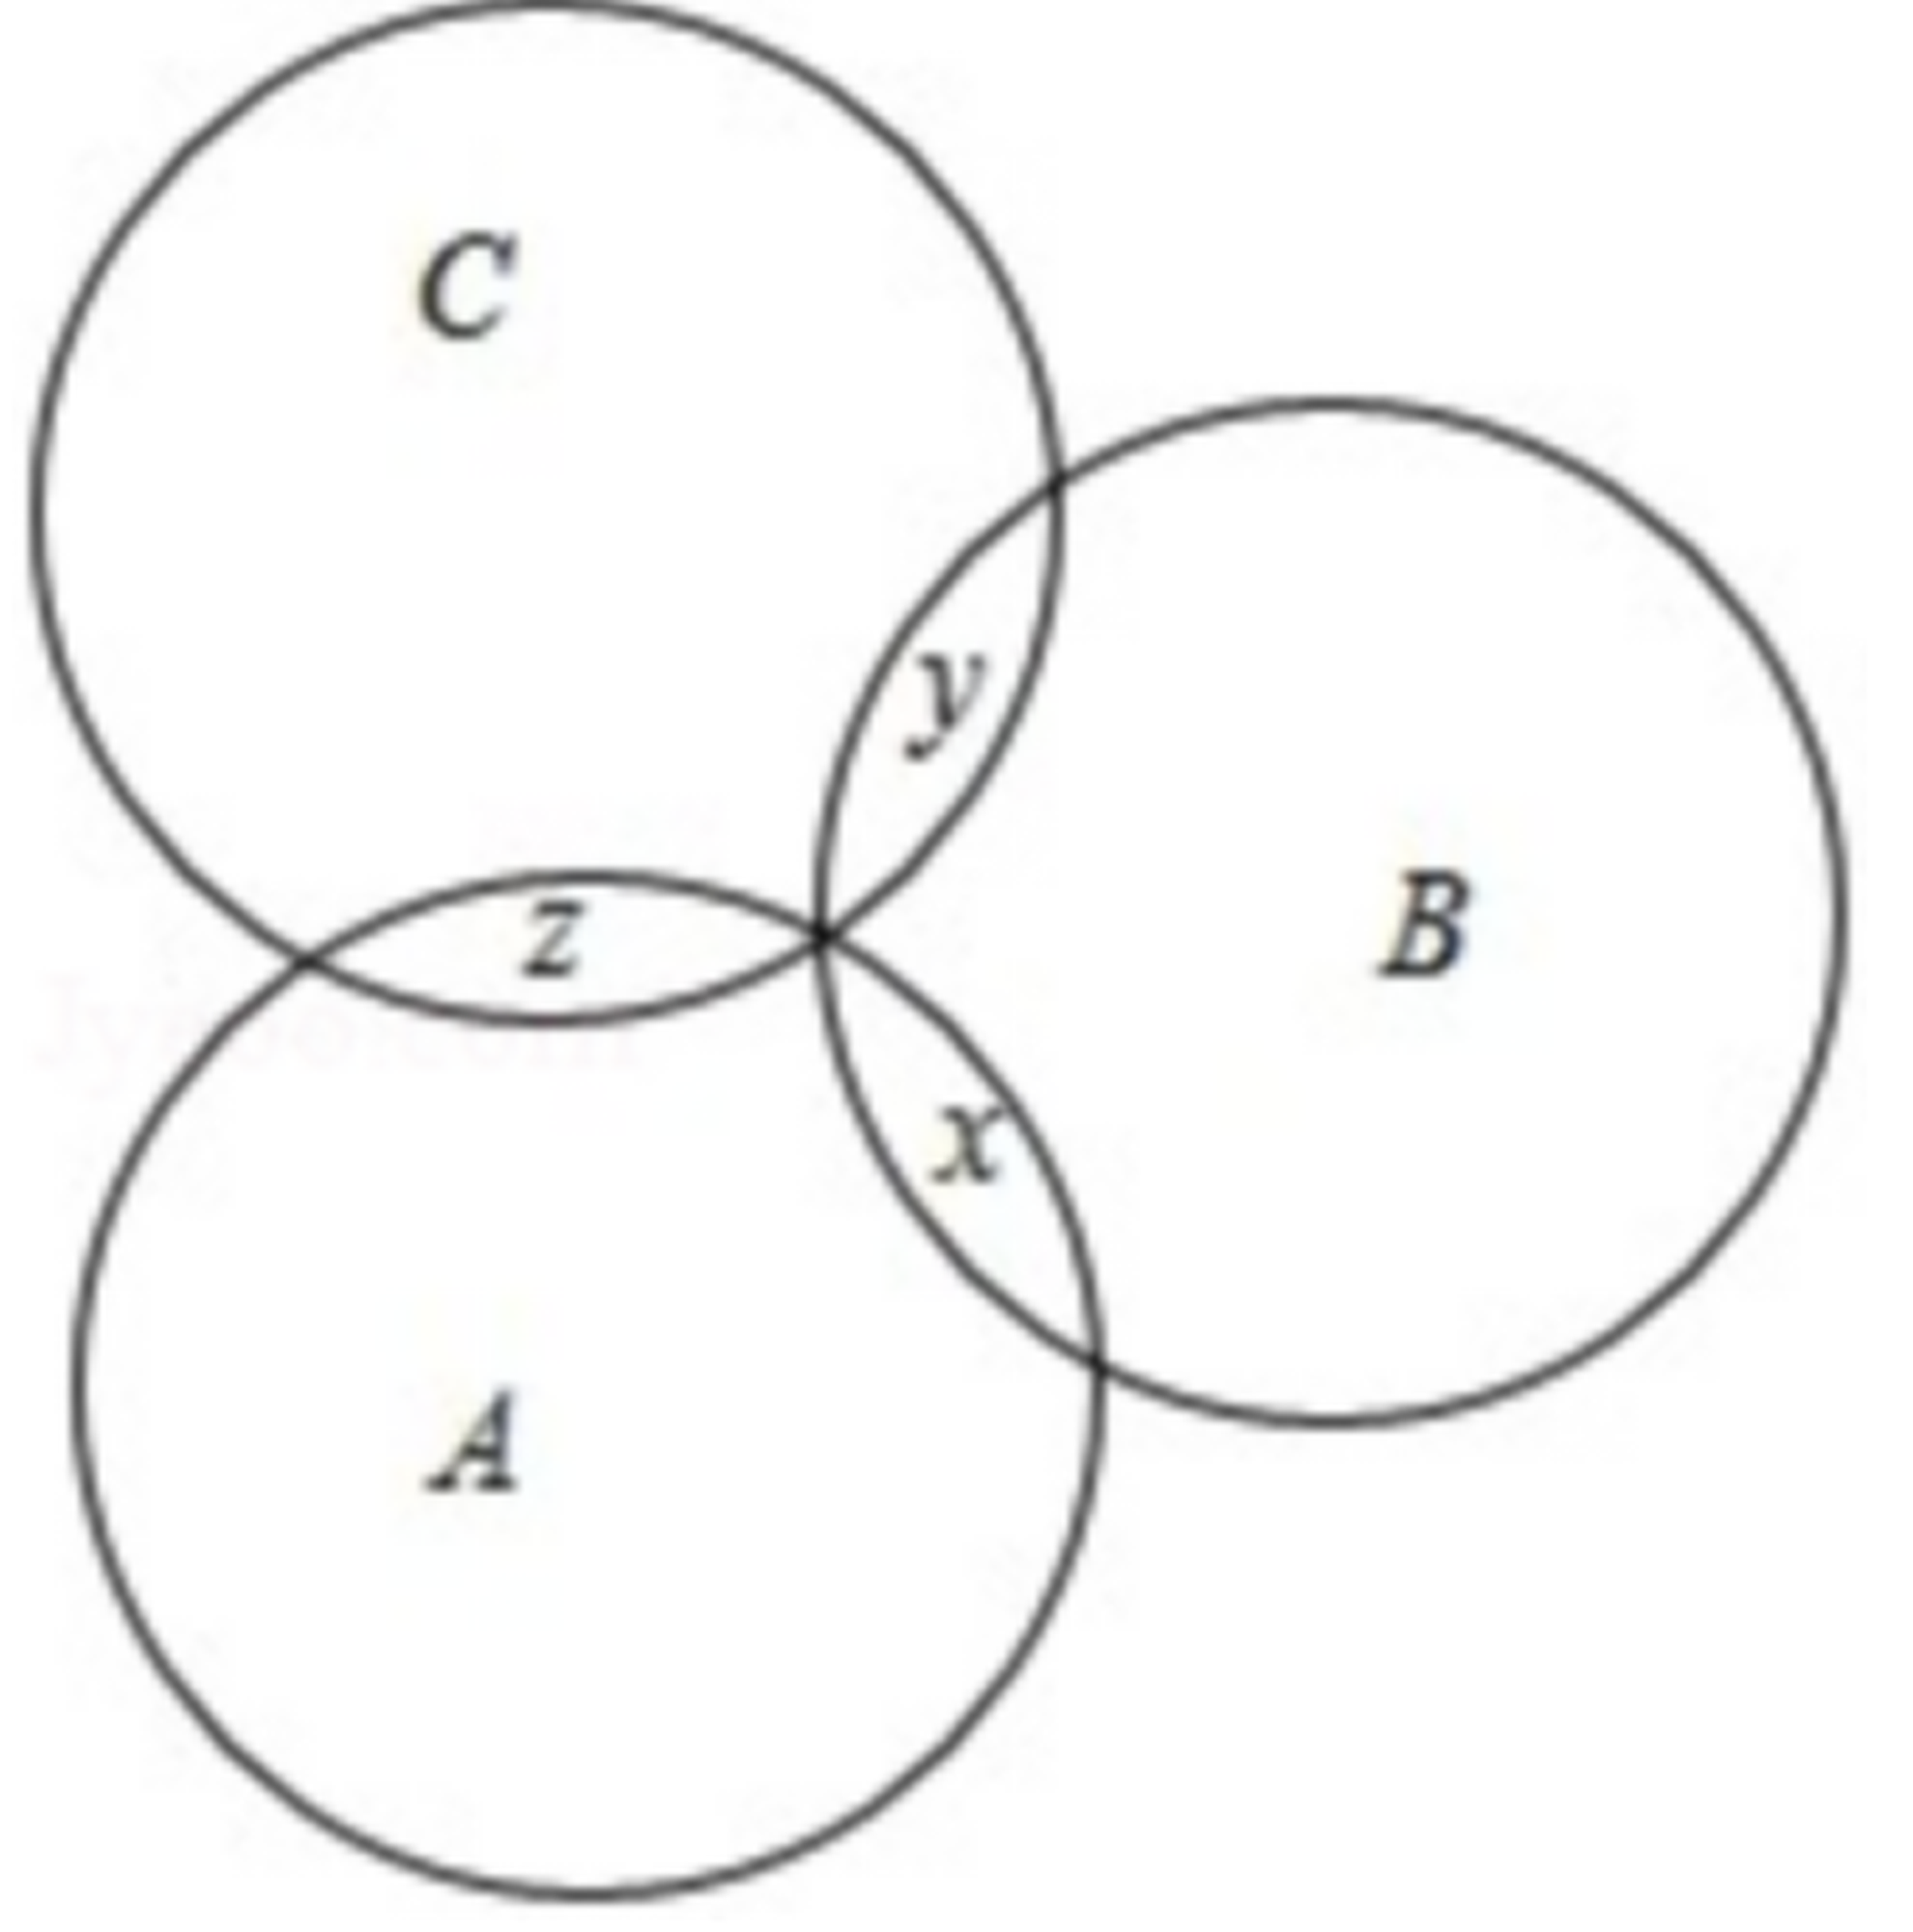
\includegraphics[width=0.30\textwidth]{figures/venn_ABC_x_y_z_h39.png}
\end{center}
\step{因为 $|A\cap B|=|B\cap C|=|C\cap A|=1$，且 $x$、$y$、$z\in\{1,2,3\}$，}
\step{所以集合 $A=\{x,z\}$，$B=\{x,y\}$，$C=\{z,y\}$，}
\step{若 $x=1$，$y=2$，$z=3$，则 $A=\{1,3\}$，$B=\{1,3\}$，$C=\{2,3\}$，}
\step{将 $1$，$2$，$3$ 进行全排列，有 $P_3^3=3\times2=6$ 个.}
\solend

\fi

\item 已知集合 $T=\{1,2,\cdots,2025\}$，对于 $T$ 的每一个非空子集的所有元素，计算它们乘积的倒数，
则所有这样倒数的和为 \blankline[4.4em].

\ans{$2025$}

\ifanswer
\solbegin
\step{集合 $T=\{1,2,\cdots,2025\}$ 的非空子集的个数为 $2^{2025}-1$，}
\step{这些子集中，每个元素的乘积分别为}
\step{$1,2,3,\cdots,2025,1\times2,1\times3,\cdots,1\times2025,\cdots,1\times2\times3\times\cdots\times2025$，}
\step{每项都可以看作是从 $1,2,3,\cdots,2025$ 中选择若干项的乘积，}
\step{$1+\dfrac12+\cdots+\dfrac{1}{2025}+\dfrac{1}{1\times2}+\dfrac{1}{1\times3}+\cdots+\dfrac{1}{2024\times2025}
+\cdots+\dfrac{1}{1\times2\times\cdots\times2025}$}
\step{$=(1+1)\left(1+\dfrac12\right)\cdots\left(1+\dfrac{1}{2025}\right)-1
=2\times\dfrac32\times\dfrac43\times\cdots\times\dfrac{2026}{2025}-1=2025$.}
\solend

\fi

% 第 24 题是压轴题，题干较长；试卷版在它之前量一次页高，尽量不与前文分家（照全稿成例）。
\ansneed{5cm}
% 注：原卷【解析】①③ 两步把 $f(x)$ 印作 $f[x[x]]$，显系笔误，照录未改，见文件头「笔误/存疑」⑦。
\item 若 $X$ 是一个集合，$T$ 是一个以 $X$ 的某些子集为元素的集合，且满足：①$X$ 属于 $T$，
$\varnothing$ 属于 $T$；②$T$ 中任意多个元素的并集属于 $T$；③$T$ 中任意多个元素的交集属于 $T$.
则称 $T$ 是集合 $X$ 上的一个拓扑. 已知函数 $f(x)=[x[x]]$，其中 $[x]$ 表示不大于 $x$ 的最大整数，
当 $x\in(0,n]$，$n\in\N^*$ 时，函数 $f(x)$ 值域为集合 $A_n$，则集合 $A_2$ 上的含有 $4$ 个元素的
拓扑 $T$ 的个数为 \blankline[4.4em].

\ans{$9$}

\ifanswer
\solbegin
\step{由题意，$n=2$，故 $0<x\leqslant2$，}
\step{①当 $0<x<1$ 时，则 $[x]=0$，所以 $f[x[x]]=0$，}
\step{②当 $x=1$ 时，$[x]=1$ 显然 $f(1)=1$，}
\step{③当 $1<x<2$ 时，$[x]=1$，所以 $f[x[x]]=[x]=1$，}
\step{④当 $x=2$ 时，$f(2)=4$，}
\step{所以 $A_2=\{0,1,4\}$，}
\step{因为 $T$ 中含有 $4$ 个元素，其中两个元素 $\varnothing$ 和 $A_2$，}
\step{$A_2=\{0,1,4\}$. 其它两个元素为 $A$、$B$，则
$\begin{cases}A\neq\varnothing\\ A\neq A_2\\ B\neq\varnothing\\ B\neq A_2\\ A\neq B\end{cases}$，}
\step{由对称性，不妨设 $1\leqslant|A|\leqslant|B|\leqslant2$，其中 $|A|$、$|B|$ 表示集合 $A$ 中元素的个数，}
\step{因为 $\begin{cases}A\cap B\in T\\ A\cup B\in T\end{cases}$，又 $|A|\leqslant|B|$，所以 $A\cap B=\varnothing$ 或 $A$，}
\step{若 $A\cap B=\varnothing$，则 $A\cup B$ 只能等于 $A_2$，}
\step{（若 $A\cup B=B$，则 $A\sub B$，则 $A\cap B=A=\varnothing$，矛盾）}
\step{则必有 $\begin{cases}|A|=1\\ |B|=2\end{cases}$，所以 $(A,B)$ 的个数 $\Leftrightarrow$ $A$ 的个数 $=3$ 种，}
\step{即 $\begin{cases}A=\{0\}\\ B=\{1,4\}\end{cases}$ 或 $\begin{cases}A=\{1\}\\ B=\{0,4\}\end{cases}$
或 $\begin{cases}A=\{4\}\\ B=\{0,1\}\end{cases}$；}
\step{若 $A\cap B=A\Leftrightarrow A\sub B$ 此时满足 $A\cup B=B$，}
\step{因为 $A\neq B$ 且 $1\leqslant|A|$ 且 $|B|\leqslant2$，所以 $\begin{cases}|A|=1\\ |B|=2\end{cases}$，}
\step{所以 $B$ 的选择共有 $C_3^2=3$ 种，则 $A$ 的个数有 $C_2^1$ 种，}
\step{所以 $(A,B)$ 的个数 $=2\times3=6$ 种.}
% 这六组「$A$／$B$」按原卷排作两行（前五个一行、第六个另起一行）；因五组并排时
% amsmath 的 cases 会为每组的第二列各留一枚 \quad，本行改排 \left\{\begin{matrix}…\end{matrix}\right.
% 以省下这枚 \quad（照 README「说明」记的高一07 成例），字形与 cases 相同。
\step{（这 $6$ 种是 $\left\{\begin{matrix}A=\{0\}\\ B=\{0,1\}\end{matrix}\right.$、
$\left\{\begin{matrix}A=\{1\}\\ B=\{0,1\}\end{matrix}\right.$、
$\left\{\begin{matrix}A=\{0\}\\ B=\{0,4\}\end{matrix}\right.$、
$\left\{\begin{matrix}A=\{4\}\\ B=\{0,4\}\end{matrix}\right.$、
$\left\{\begin{matrix}A=\{1\}\\ B=\{1,4\}\end{matrix}\right.$、}
\step{$\left\{\begin{matrix}A=\{4\}\\ B=\{1,4\}\end{matrix}\right.$）.}
\step{综上，$T$ 的个数为 $9$ 个.}
\solend

\fi

\end{enumerate}

\end{document}
"
% 紧凑版：xelatex "\def\iscompact{1}% 高一39_大同中学_周末作业4.1.tex
%   —— 高一上数学「2026-2027 年大同中学高一上周末作业 4.1」（试卷版/答案版）
% 试卷版：xelatex 高一39_大同中学_周末作业4.1.tex
% 答案版：xelatex "\def\isanswer{1}\input{高一39_大同中学_周末作业4.1.tex}"
% 紧凑版：xelatex "\def\iscompact{1}\input{高一39_大同中学_周末作业4.1.tex}"
%
% 原始材料是微信公众号图文（公众号「魔都数学加油站」连载「27学年高一 39」，署名「破晓」，
% 2026-09-26 21:29 发布，原文标题「27学年高一39——2026-2027年上海市大同中学高一上周末作业4.1」，
% 原文链接 https://mp.weixin.qq.com/s/HR2hIayXUXNi4zTs3PioiQ ），正文为 11 张 PNG 页。**同一篇里各页分辨率不一致**（2560×3620 与 4762×6735 两档混排：第 1、3、8、10 页为
% 2560×3620，第 2、4、5、6、7、9、11 页为 4762×6735）。原文本身就是一份**讲评版**——除第 15 题
% 外各题题下直接印【解析】（无单独的【答案】行），第 15 题的答案「D」直接印在题干末尾的括号内。
% 试题文字、答案与解析均照原卷录入，未改内容。卷面的粉色斜水印「魔都数学加油站」属水印，未录入。
%
% 卷首标题：原卷页首印作「2026-2027 年大同中学高一上周末作业 4.1」（**卷面标题行即带校名**，
% 年份区间按全稿惯例排 en dash，前缀照原卷保留「年」）。
%
% 篇幅与题号：卷面自「一、填空题」的**第 3 题**起编，终于「附加题」的**第 24 题**，共 22 题
% （填空 3—12、选择 13—16、解答 17—20、附加题 21—24）。第 1、2 题未在该文中发布——这是该
% 公众号连载讲评版的通例（高一02—高一09 等均自第 3 题起编，README「说明」已记），**不是截断**，
% 故本稿题号亦自 3 起。它与 高一40（大同中学 周末作业4.2）同属「周末作业 4」系列但**各自独立起编**
% （4.2 自第 3 题起、终于第 19 题），不是同一份试卷的两半。
%
% 与原卷的排版差异（均已在 README「说明」中交代）：
%   ① 原文自**第 3 题**起（第 1、2 题未在该文中发布），故本稿题号亦自 3 起，填空题以
%      \setcounter{enumi}{2} 起编；选择、解答、附加题三节各按上一节末号另设 \setcounter
%      （选择题 \setcounter{enumi}{12}、解答题 \setcounter{enumi}{16}、附加题 \setcounter{enumi}{20}）；
%   ② 原卷本就印有「一、填空题」「二、选择题」「三、解答题」三节标题，末节印作「附加题」
%      （**不带「四、」**，且题号 21—24 续前编、不另起），本稿照原卷分节，只把标题改排成全稿
%      统一的「大节标题」样式；
%   ③ 原卷是「讲评版」：除第 15 题外，各题题下均印【解析】（**全卷无一条独立的【答案】行**）；
%      第 15 题无解析，答案「D」直接印在题干末尾的括号内。本稿统一改为试卷版隐去、答案版以
%      \ans{}／\ifanswer 块给出，两版彻底分离；原卷写在【解析】末句的结果，本稿照 高一38
%      （同校同系列、同为讲评版）的成例另提为 \ans{}；
%   ④ 数集记号原卷两套并用：实数集作斜体的 $R$（第 7、11、14、17、18、19 题），整数集作斜体
%      $Z$（第 10 题），自然数集作斜体 $N$ 及 $N^*$（第 16、20、21、24 题），本稿按全稿惯例
%      统一写作 $\R$、$\Z$、$\N$、$\N^*$；
%   ⑤ 补集符号原卷两套并用：第 7 题作前缀式的 $C_U$（且题干称全集为 $I$，见「笔误/存疑」①），
%      第 14、15、18 题作上横线（$\overline{H}$、$\overline{A}$、$\overline{B}$），本稿照录、不归一
%      （前缀式写作 $\complement_U$，与 高一c／高一10 的成例一致）；
%   ⑥ 包含符号原卷两套并用：第 3 题作**无下划线**的 $\subset$，第 15、18、20、24 题作**带下划线**
%      的 $\sub$，本稿照录、不归一；
%   ⑦ 原卷填空的横线约两个字宽，本稿按全稿惯例统一排 \blankline[4.4em]；
%   ⑧ 第 7、11、22 题各有插图，取原卷截图、4× LANCZOS 放大（figures/venn_N_cap_CI_M_h39.png、
%      figures/plane_grid_4squares_h39.png、figures/venn_ABC_x_y_z_h39.png）；第 7 题的 Venn 属
%      **题干**（试卷版、答案版都出），第 11、22 题的图在【解析】内（仅答案版出）。第 7 题图
%      左下、第 11 题图的上／左／右边缘带进极淡的原卷粉色水印残影——照全稿「插图直接取自
%      原卷截图、不用 TikZ 重绘、不修图」的体例保留（再裁会切到坐标轴与 $x$、$y$、$O$ 标注）；
%   ⑨ 原卷并列的字母、数字（「$x_1,x_2$」「$a,b$」「$1,2,3,\cdots,11$」）多作半角逗号或不加标点，
%      本稿按全稿惯例改排顿号（$x_1$、$x_2$）或把数列并入行内公式；半角括号、逗号一律排全角，
%      数学式内部的标点照原样；
%   ⑩ 原卷未印副标题，本稿按**本卷实际内容**补出副标题「集合与常用逻辑用语」（依据见下条）。
%
% 副标题（\examtitlest 第二个参数）：本卷卷面未印副标题，由本稿补出，取值按 2026-09-26 起的
%   新口径「只用本卷实际内容的模块名」定为「集合与常用逻辑用语」。依据：全卷 22 题（第 3—24 题）中，
%   第 3、5、7、8、10、11、14、15、16、17、18、19、20、21、22、23、24 题共 17 题是集合的运算与
%   关系、子集／真子集、补集、集合新定义（「全食／偏食」、最小相交、拓扑、特征数）与集合计数，
%   以及命题与常用逻辑用语（第 3 题充要条件、第 5 题存在量词命题、第 17 题命题真假）；其余两题
%   第 4、6 考一元二次方程的根（韦达定理）与方程恒等，第 9、12、13 题是不等式（一元二次不等式组
%   的整数解、一元二次不等式解集、不等式的性质）——不等式合计 3/22，**不足全卷三分之一**，
%   故不并标「不等式」。
%
% 原卷笔误/存疑（均照抄原卷、未改，见源码中该处上方注释）：
%   ① 第 7 题题干称「全集 $I=R$」，而【解析】两处把补集写作 $C_U M$（下标作 $U$），前后记号不一；
%      本稿照录，未改；
%   ② 第 4 题【解析】两处把判别式印作 $\triangle=[2(m-1)^2-16m^2]$（方括号内首项漏了平方，
%      正确应作 $[2(m-1)]^2-16m^2$）；按其所判「$m=\frac12$ 时 $<0$、$m=-\frac12$ 时 $>0$」反推，
%      $[2(m-1)]^2-16m^2$ 在 $m=\frac12$ 时为 $-3<0$、在 $m=-\frac12$ 时为 $5>0$，与结论一致；
%      本稿照录；
%   ③ 第 9 题【解析】把方程组第二式印作 $1-2<-k\leqslant3$，按其结论 $-3\leqslant k<2$ 反推，
%      疑当作 $-2<-k\leqslant3$（原卷多一个「$1$」）；本稿照录；
%   ④ 第 17 题【解析】首句「由数 $y=-x^2+ax-1=-x+3$」中的「由数」显系「由」或「由函数」之误；
%      且末段「若 $p$ 真 $q$ 假…得 $a\in R$」「若 $p$ 假 $q$ 真…此时 $a$ 无解」与结论「$a$ 的取值范围
%      是 $R$」自相矛盾（按 $p:a\leqslant-5$、$q:a>-6$，$p$ 真 $q$ 假应为 $a\leqslant-6$，$p$ 假 $q$ 真
%      应为 $a>-5$，合起来是 $a\leqslant-6$ 或 $a>-5$，并非 $R$）；本稿一律照录，未按正确解法改写；
%   ⑤ 第 18 题【解析】(2) 把 $B=\{x\mid x^2+a\leqslant0\}$（$a<0$）印作右端开的
%      $\{x\mid-\sqrt{-a}\leqslant x<\sqrt{-a}\}$（应为闭的「$\leqslant$」）；按其所判
%      $\sqrt{-a}<\frac12$ 反推，不影响结论；本稿照录；
%   ⑥ 第 22 题【解析】在 $x=1$、$y=2$、$z=3$ 时把 $B=\{x,y\}$ 印作 $\{1,3\}$（应为 $\{1,2\}$），
%      与本行前面「$B=\{x,y\}$」不合；本稿照录；
%   ⑦ 第 24 题【解析】①③ 两步把 $f(x)$ 印作 $f[x[x]]$，显系笔误；本稿照录。
%   ⑧ 第 8 题【解析】「即方程 $x^2+ax+b=x$，$x^2+(a-1)x+b=0$ **由**两个相等的实数根为 $4$」——
%      「由」当为「有」（「设…是…有」的杂糅）；本稿照录；
%   ⑨ 第 10 题：题设 $a\oplus b=b(a^2+b^2+1)$，而集合定义里含 $\dfrac{a\oplus b}{2b}$；$-2<a<b<2$、
%      $a$、$b\in\Z$ 时 $(a,b)=(-1,0)$ 也合条件、却使分母 $2b=0$，原卷解析仍代入该组并约去
%      $b$ 得 $x=1$（答案集恰好不变）；本稿照录；
%   ⑩ 第 15 题选项列里 ② 与 ③ 之间**漏排分隔号**（原卷作「② $\overline{A}\cap B=\varnothing$③
%      $\overline{A}\sub\overline{B}$；」——①、③ 后都有「；」，② 后没有）；本稿照录；
%   ⑪ 第 20(2) 把 $\{1,2,\cdots,20\}$ 分成的 11 个集合里，$\{8,11\}$ 与 $\{9,12\}$ 之间误用
%      **句号**「.」（同行其余处皆逗号）；本稿照录；
%   ⑫ 第 20(3)① 推理不严：原卷写「选 5 则不选 1、9；选 6 则不选 2、10；选 7 则不选 3、11；
%      则只剩 4、8」——但 4 与 8 相差 $4$、不能同选，该情形实际最多只能取 $4$ 个；末句结论
%      「不超过 $5$ 个」仍成立；本稿照录；
%   ⑬ 第 16 题【解析】两种下标并存：「所以在 $A_i$ 的特征数构成中」原卷作斜体 $A_i$，而
%      「要使 $X_1+X_2+X_3$ 最大（小），则（应）在集合 $A_1$ 中首先放置…」两处原卷作
%      **数字 $1$**（与同句 $X_1$ 的角标同形）；本稿照录、未归一。
%
% 图取原卷截图（依次见各处的 \includegraphics 前的注释），4× LANCZOS 放大。
\documentclass[a4paper,11pt]{article}
\usepackage{common}

\begin{document}

\examtitlest[3]{2026--2027 年大同中学高一上周末作业 4.1}{集合与常用逻辑用语}

\bigsec{一、填空题}

\begin{enumerate}
\setcounter{enumi}{2}

\item “$x\geqslant a$”是“$0<x<2$”的必要非充分条件，则实数 $a$ 的取值范围是 \blankline[4.4em].

\ans{$(-\infty,0]$}

\ifanswer
\solbegin
\step{因为 $x\geqslant a$ 是 $0<x<2$ 的必要非充分条件，所以 $(0,2)\subset[a,+\infty)$，所以 $a\leqslant0$，}
\step{则实数 $a$ 的取值范围是 $(-\infty,0]$.}
\solend

\fi

% 注：原卷$[2(m-1)^2-16m^2]$ 首项漏了平方（应为 $[2(m-1)]^2-16m^2$），照录未改，见文件头「笔误/存疑」②。
\item 若关于 $x$ 的方程 $x^2+2(m-1)x+4m^2=0$ 有两个实数根，且这两根互为倒数，则 $m=$ \blankline[4.4em].

\ans{$-\dfrac12$}

\ifanswer
\solbegin
\step{设 $x_1$、$x_2$ 是方程 $x^2+2(m-1)x+4m^2=0$ 有两个实数根，}
\step{则 $x_1x_2=4m^2=1$，解得 $m=\dfrac12$ 或 $m=-\dfrac12$，}
\step{又当 $m=\dfrac12$ 时，$\triangle=[2(m-1)^2-16m^2]<0$，舍去，}
\step{当 $m=-\dfrac12$ 时，$\triangle=[2(m-1)^2-16m^2]>0$，故 $m=-\dfrac12$.}
\solend

\fi

\item 已知命题：“存在 $x\in[1,2]$，使 $x^2+2x+a\geqslant0$”为真命题，则 $a$ 的取值范围是 \blankline[4.4em].

\ans{$a\geqslant-8$}

\ifanswer
\solbegin
\step{若存在 $x\in[1,2]$，使 $x^2+2x+a\geqslant0$，}
\step{则等价为存在 $x\in[1,2]$，使 $x^2+2x\geqslant-a$，}
\step{当存在 $x\in[1,2]$ 时，设 $y=x^2+2x=(x+1)^2-1$，则 $3\leqslant y\leqslant8$，}
\step{所以要使 $x^2+2x\geqslant-a$，则 $8\geqslant-a$，即 $a\geqslant-8$.}
\solend

\fi

\item 已知方程 $a(3x+2)+b(2x-3)=8x+3$ 有无穷多个解，则 $a:b=$ \blankline[4.4em].

\ans{$30:7$}

\ifanswer
\solbegin
\step{$a(3x+2)+b(2x-3)=(3a+2b)x+2a-3b=8x+3$ 有无穷多个解，}
\step{所以 $\begin{cases}3a+2b=8\\ 2a-3b=3\end{cases}$，解得 $a=\dfrac{30}{13}$，$b=\dfrac{7}{13}$，所以 $a:b=30:7$.}
\solend

\fi

% 注：原卷题干称「全集 $I=R$」，而【解析】两处把补集写作 $C_U M$（下标作 $U$），前后记号不一；
%     照录未改，见文件头「笔误/存疑」①。
\item 已知集合 $M=\{x\mid y=\sqrt{3-x^2}\}$，$N=\{x\mid-3\leqslant x\leqslant1\}$，全集 $I=\R$，
则图中阴影部分表示的集合为 \blankline[4.4em].

% 图取原卷截图（01.png，2560×3620）右栏，4× LANCZOS 放大。
\begin{center}
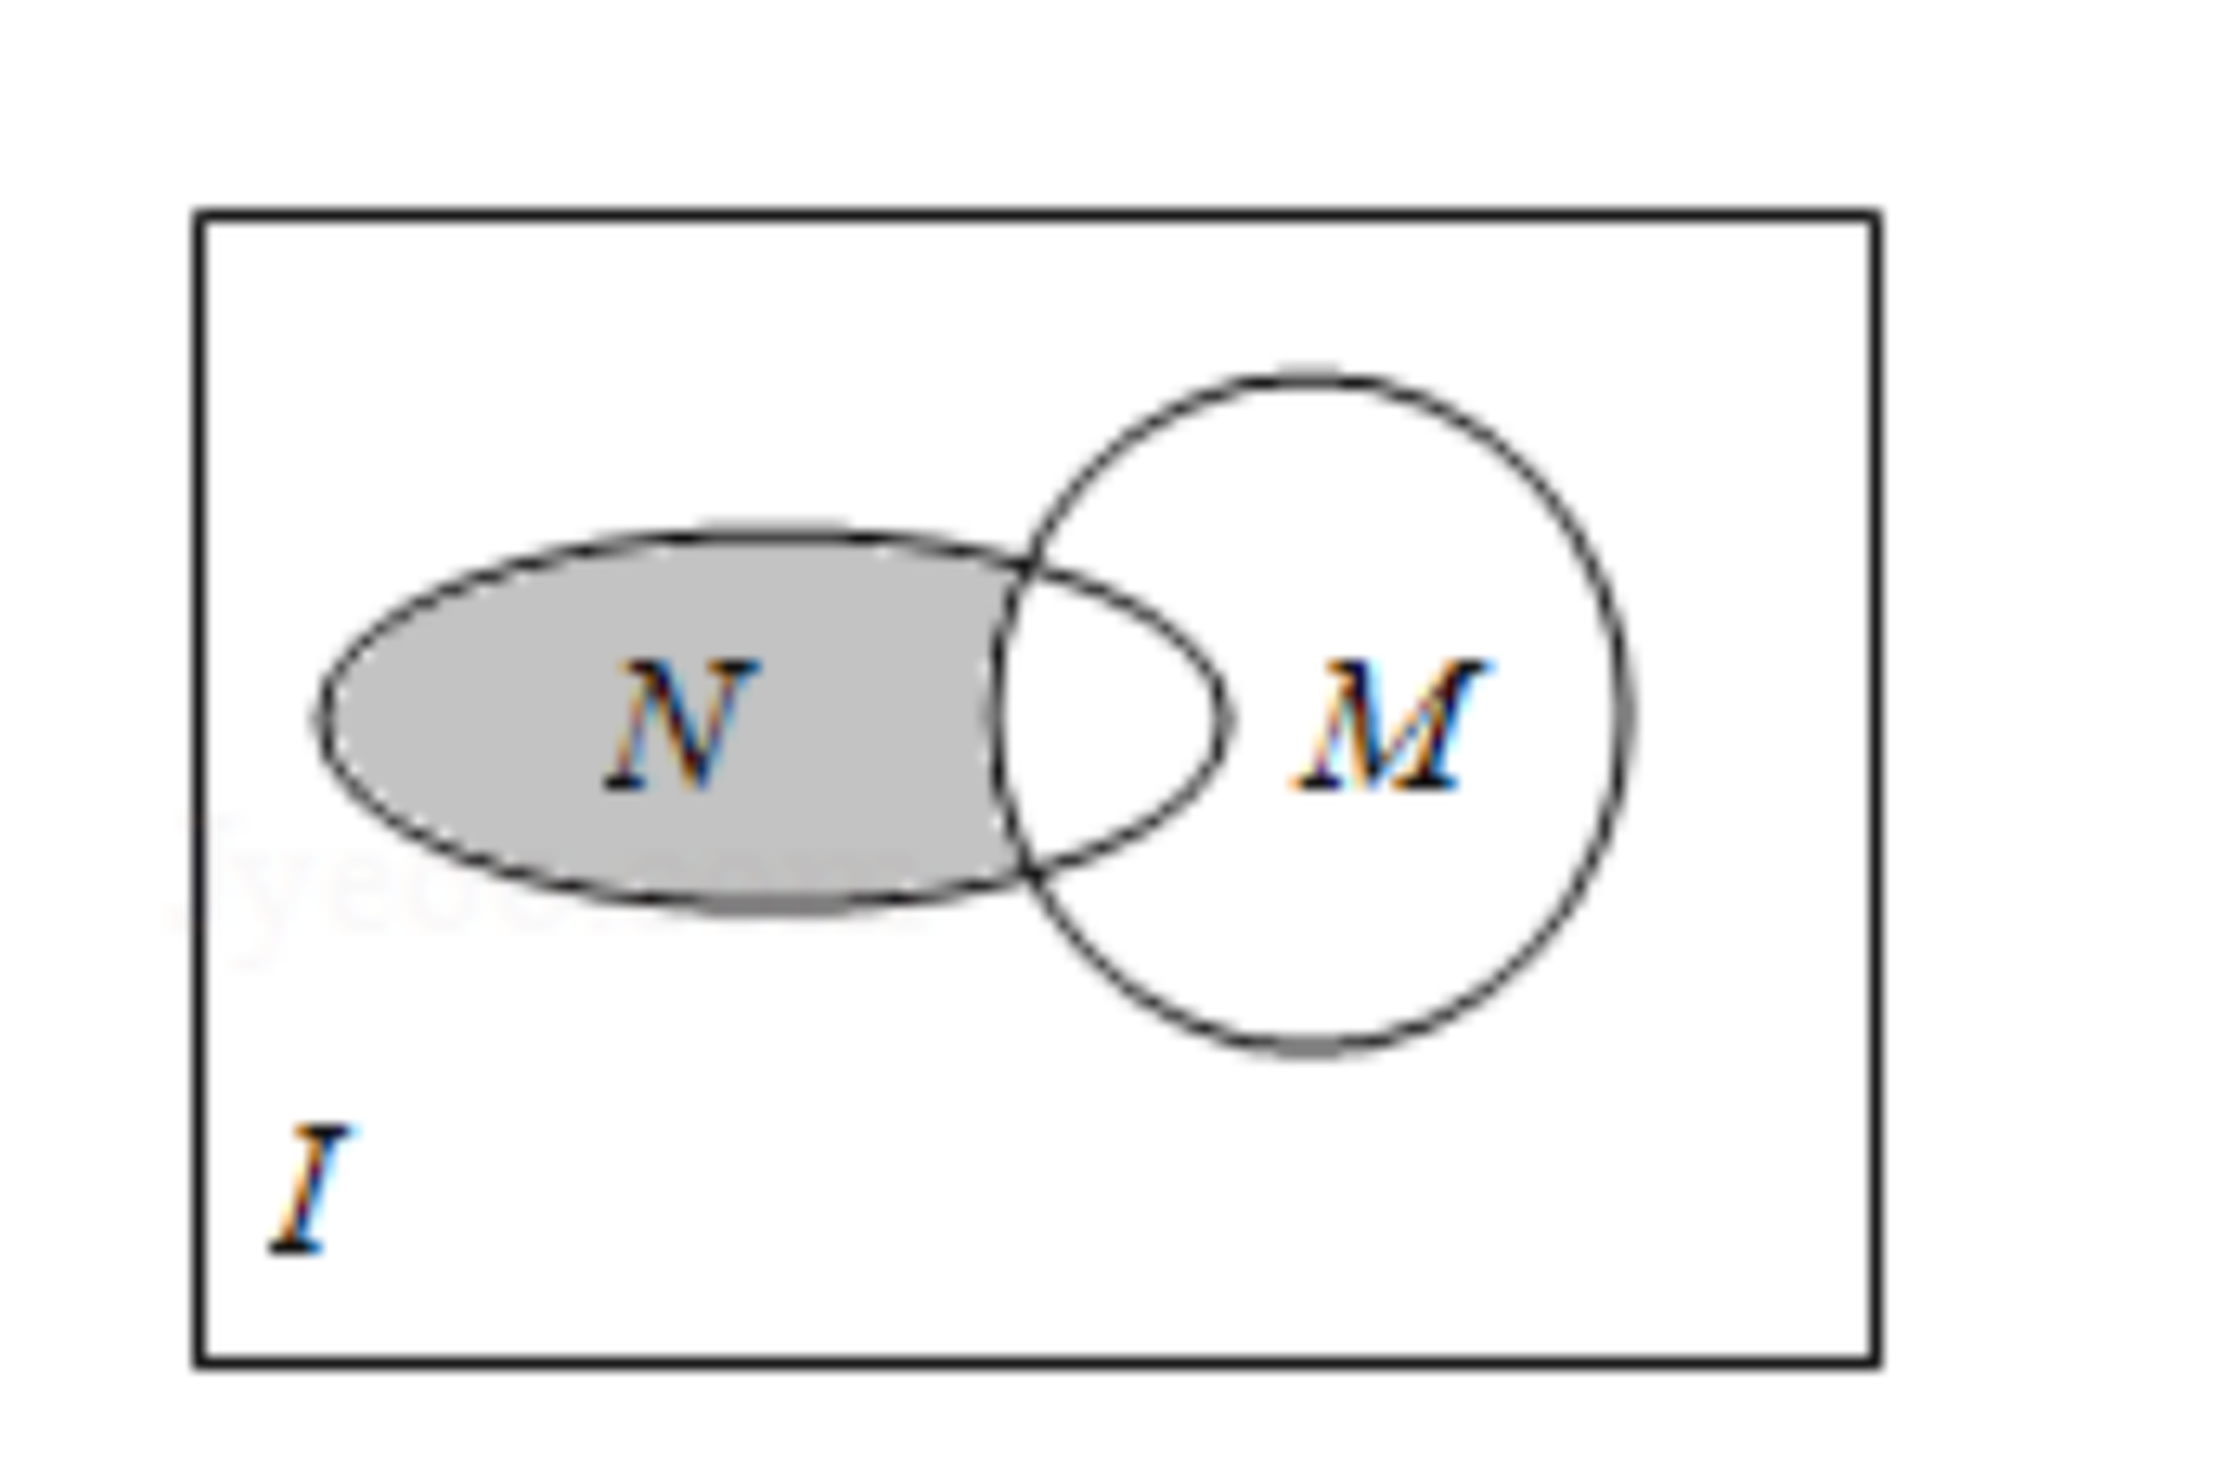
\includegraphics[width=0.30\textwidth]{figures/venn_N_cap_CI_M_h39.png}
\end{center}

\ans{$[-3,-\sqrt3)$}

\ifanswer
\solbegin
\step{阴影部分用集合表示为 $N\cap(\complement_UM)$.}
\step{则 $M=\{x\mid y=\sqrt{3-x^2}\}=\{x\mid3-x^2\geqslant0\}=\{x\mid-\sqrt3\leqslant x\leqslant\sqrt3\}$，}
\step{则 $\complement_UM=\{x\mid x>\sqrt3\text{ 或 }x<-\sqrt3\}$，$N=\{x\mid|x+1|\leqslant2\}=\{x\mid-3\leqslant x\leqslant1\}$，}
\step{则 $N\cap(\complement_UM)=\{x\mid-3\leqslant x<-\sqrt3\}$.}
\solend

\fi

\item 已知 $f(x)=x^2+ax+b$，集合 $\{x\mid f(x)=x\}=\{4\}$，将集合 $M=\{x\mid f(x)=4\}$ 用列举法表示 \blankline[4.4em].

\ans{$\{3,4\}$}

\ifanswer
\solbegin
\step{已知 $f(x)=x^2+ax+b$，集合 $\{x\mid f(x)=x\}=\{4\}$，}
% 注：原卷本行作「…$x^2+(a-1)x+b=0$ **由**两个相等的实数根为 $4$」——「由」当为「有」
%     （「设…是…有」的杂糅）；本稿照录未改，见文件头「原卷笔误/存疑」⑧。
\step{即方程 $x^2+ax+b=x$，$x^2+(a-1)x+b=0$ 由两个相等的实数根为 $4$，}
\step{所以 $\triangle=(a-1)^2-4b=0$，即 $x^2+(a-1)x+b=(x-4)^2$，所以 $b=16$，$a=-7$，}
\step{所以 $f(x)=x^2+ax+b=x^2-7x+16$，所以集合 $M=\{x\mid f(x)=4\}$，}
\step{即 $x^2-7x+16=4$，$x^2-7x+12=0$，故 $M=\{x\mid f(x)=4\}=\{3,4\}$.}
\solend

\fi

% 注：原卷方程组第二式印作 $1-2<-k\leqslant3$，按其结论 $-3\leqslant k<2$ 反推疑当作 $-2<-k\leqslant3$，
%     照录未改，见文件头「笔误/存疑」③。
\item 关于 $x$ 的不等式组 $\begin{cases}x^2-x-2>0\\ 2x^2+(2k+5)x+5k<0\end{cases}$ 的整数解的集合为 $\{-2\}$，
则实数 $k$ 的取值范围 \blankline[4.4em].

\ans{$-3\leqslant k<2$}

\ifanswer
\solbegin
\step{原不等式组即 $\begin{cases}(x-2)(x+1)>0\\ (x+k)(2x+5)<0\end{cases}$，整数解的集合为 $A$，若 $A=\{-2\}$，}
\step{则 $(-2+k)(2\times(-2)+5)<0$，所以 $k<2$，且有 $\begin{cases}-k>-\dfrac52\\ 1-2<-k\leqslant3\end{cases}$，}
\step{解得 $-3\leqslant k<2$.}
\solend

\fi

\item 规定 $\oplus$ 与 $\otimes$ 是两个运算符号，其运算法则如下，对任意实数 $a$、$b$ 有：$a\otimes b=ab$，
$a\oplus b=b(a^2+b^2+1)$. 若 $-2<a<b<2$ 且 $a$、$b\in\Z$，
$A=\left\{x\mid x=2(a\otimes b)+\dfrac{a\oplus b}{2b}\right\}$，则用列举法表示集合 $A=$ \blankline[4.4em].

\ans{$\left\{1,-\dfrac12\right\}$}

\ifanswer
\solbegin
\step{$A=\left\{x\mid x=2(a\otimes b)+\dfrac{a\oplus b}{2b}\right\}
=\left\{x\mid x=2ab+\dfrac{b(a^2+b^2+1)}{2b}\right\}$}
\step{$=\left\{x\mid x=2ab+\dfrac12a^2+\dfrac12b^2+\dfrac12\right\}
=\left\{x\mid x=\dfrac12(a+b)^2+ab+\dfrac12\right\}$，}
% 注：题设含 $\dfrac{a\oplus b}{2b}$，而 $-2<a<b<2$、$a$、$b\in\Z$ 时 $(a,b)=(-1,0)$ 也合条件、
%     却使分母 $2b=0$；原卷解析仍代入该组并约去 $b$ 得 $x=1$（答案集恰好不变）。本稿照录，
%     见文件头「原卷笔误/存疑」⑨。
\step{当 $a=-1$，$b=0$ 时，$x=1$；当 $a=-1$，$b=1$ 时，$x=-\dfrac12$；}
\step{当 $a=0$，$b=1$ 时，$x=1$；所以 $A=\left\{1,-\dfrac12\right\}$.}
\solend

\fi

\item 高斯是德国著名的数学家，近代数学奠基者之一，享有“数学王子”的称号，为了纪念数学家高斯，
我们把取整函数 $y=[x]$，$x\in\R$ 称为高斯函数，其中 $[x]$ 表示不超过 $x$ 的最大整数，
如 $[1.1]=1$，$[-1.1]=-2$. 则点集 $P=\{(x,y)\mid[x]^2+[y]^2=1\}$
所表示的平面区域的面积是 \blankline[4.4em].

\ans{$4$}

\ifanswer
\solbegin
\step{$[x]^2+[y]^2=1$ 由 $\begin{cases}[x]=0\\ [y]=-1\end{cases}$ 或 $\begin{cases}[x]=0\\ [y]=1\end{cases}$
或 $\begin{cases}[x]=-1\\ [y]=0\end{cases}$ 或 $\begin{cases}[x]=1\\ [y]=0\end{cases}$ 四个平面区域组成，}
\step{即 $\begin{cases}0\leqslant x<1\\ -1\leqslant y<0\end{cases}$ 或 $\begin{cases}0\leqslant x<1\\ 1\leqslant y<2\end{cases}$
或 $\begin{cases}-1\leqslant x<0\\ 0\leqslant y<1\end{cases}$ 或 $\begin{cases}1\leqslant x<2\\ 0\leqslant y<1\end{cases}$，}
\step{作出平面区域如图所示，平面区域由四个边长为 $1$ 的正方形组成，}
% 图在【解析】内（仅答案版出），取原卷截图（03.png，2560×3620）中部，4× LANCZOS 放大。
\begin{center}
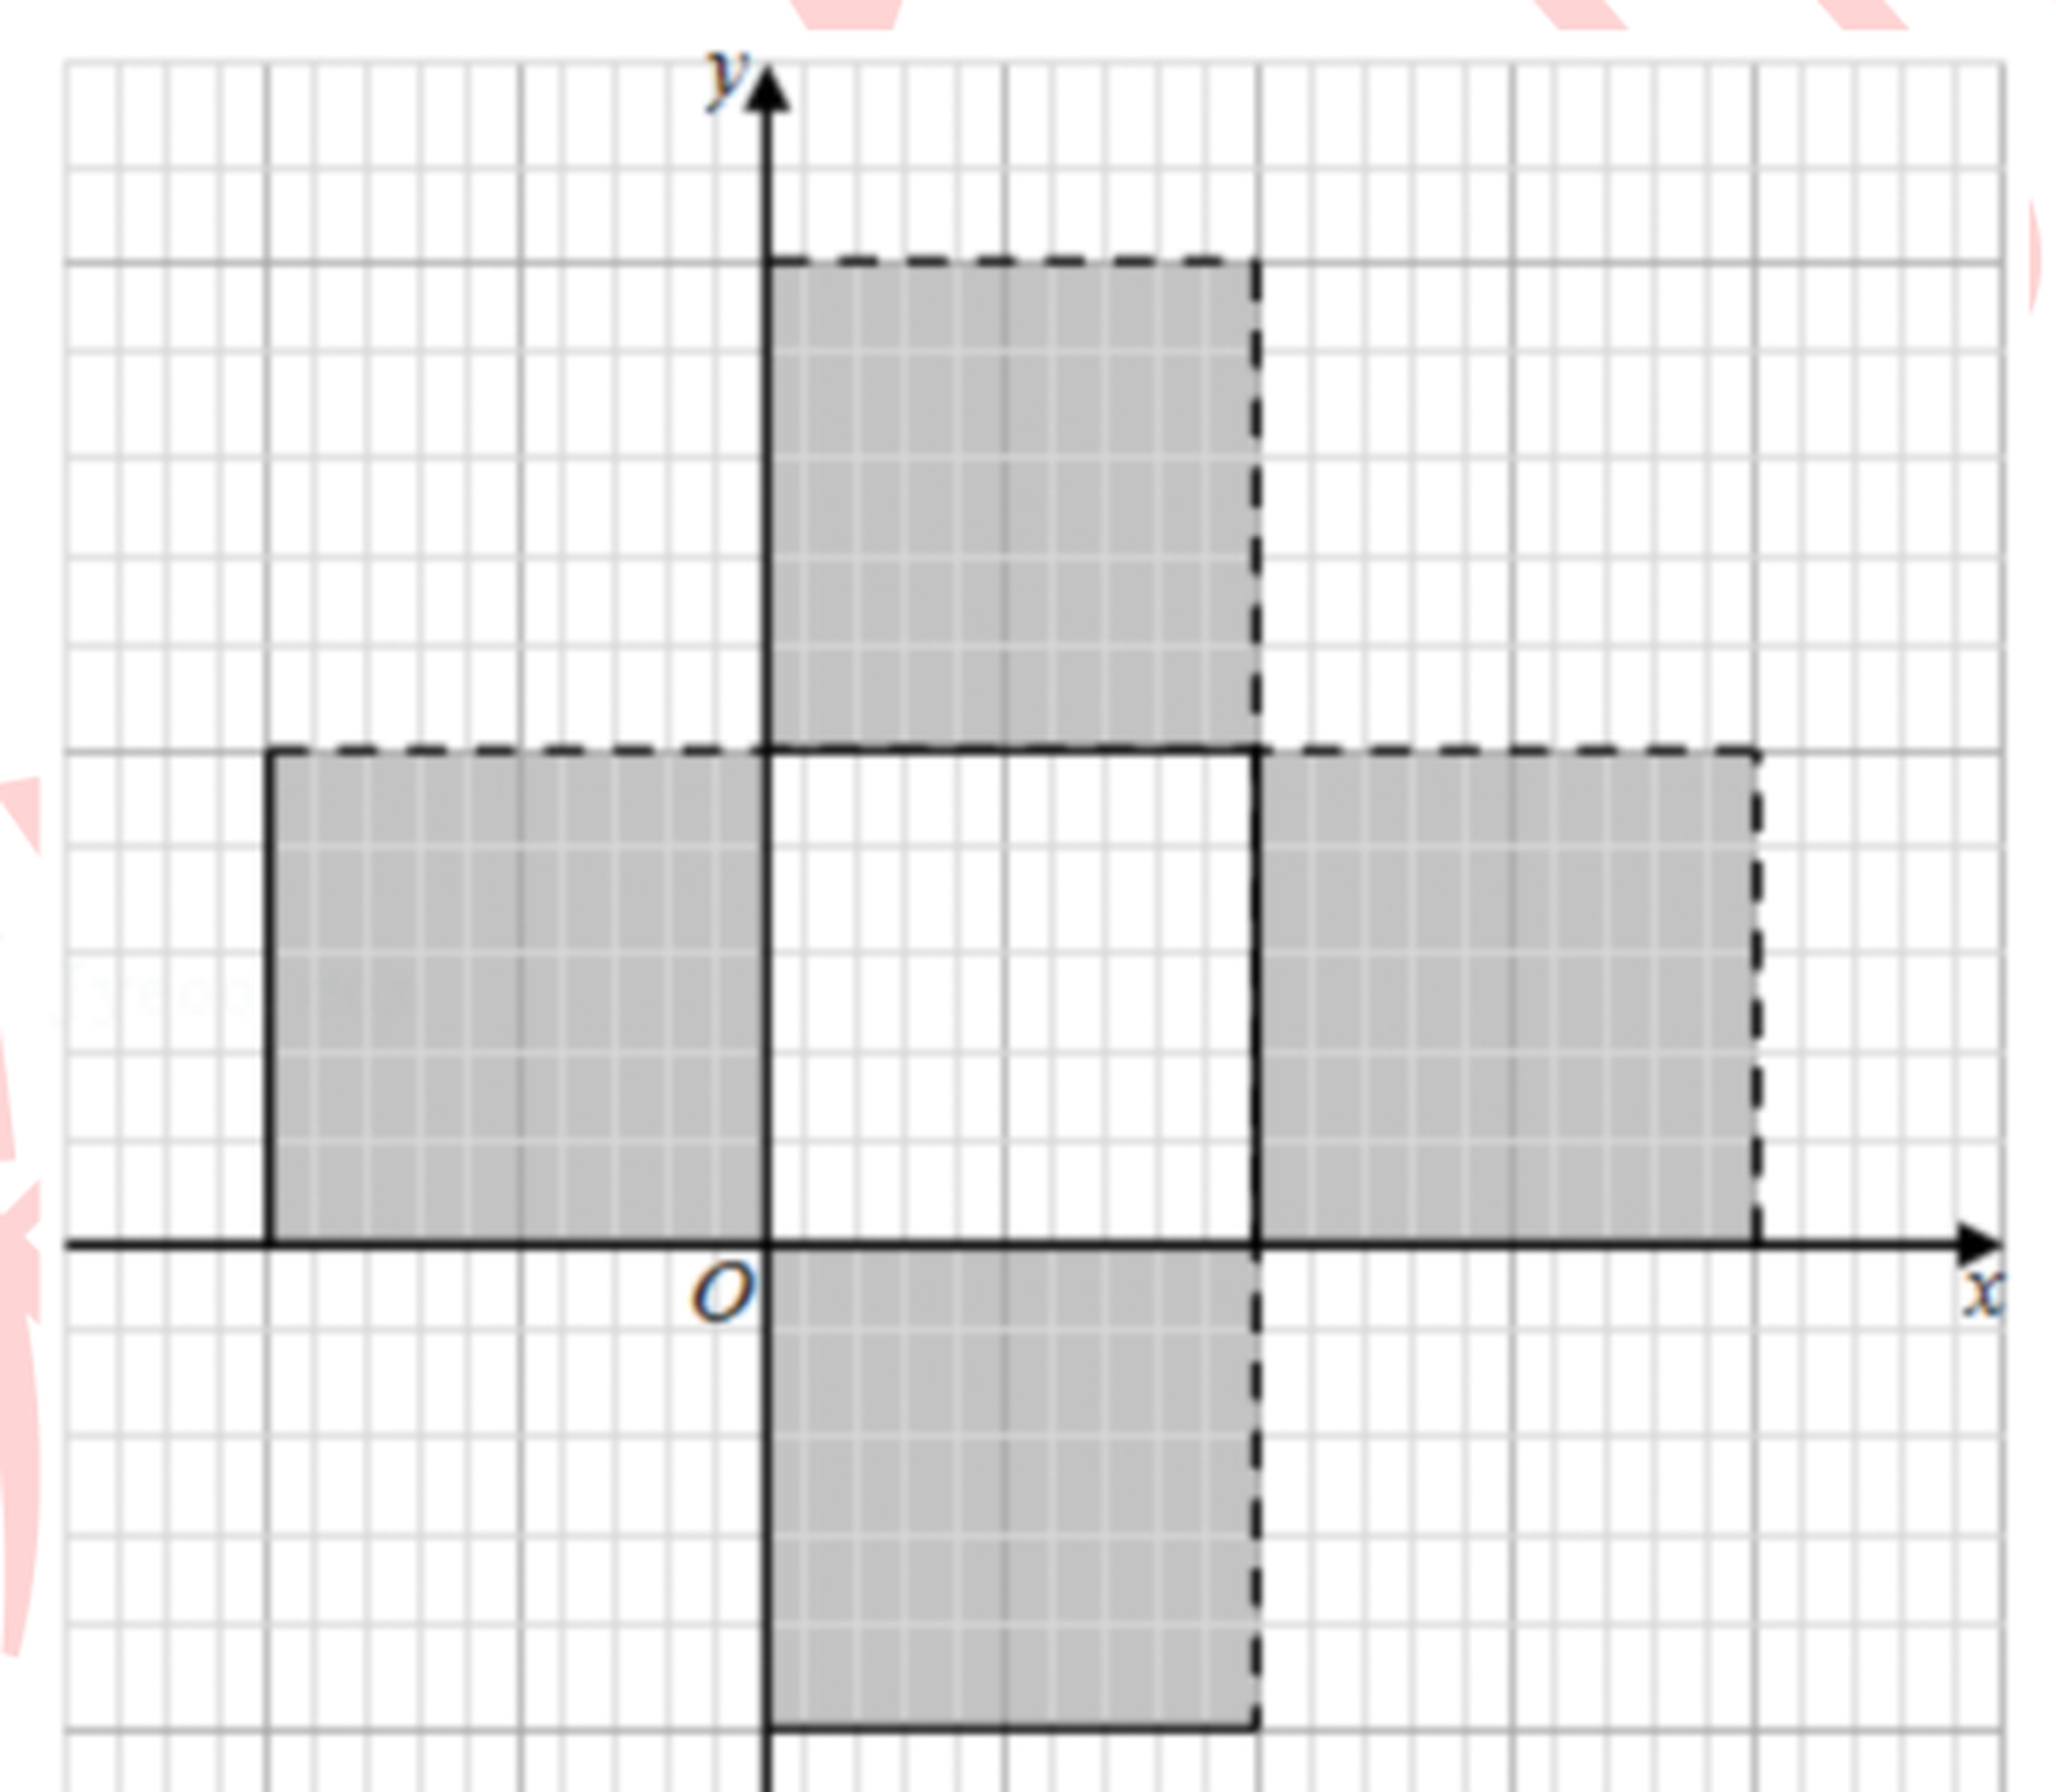
\includegraphics[width=0.38\textwidth]{figures/plane_grid_4squares_h39.png}
\end{center}
\step{总面积为 $1\times4=4$.}
\solend

\fi

\item 关于 $x$ 的不等式 $ax^2+bx+c>0$ 的解集为 $\{x\mid x<\beta\text{ 或 }x>\gamma\}(0<\beta<\gamma)$，
则不等式 $a(x^2+1)+b(x-1)+c>2ax$ 的解集为 \blankline[4.4em].

\ans{$(-\infty,\beta+1)\cup(\gamma+1,+\infty)$}

\ifanswer
\solbegin
\step{由题意得 $\beta$、$\gamma$ 为方程 $ax^2+bx+c=0$ 的两根且 $a>0$，}
\step{则 $\beta+\gamma=-\dfrac ba$，$\beta\gamma=\dfrac ca$，故 $b=-a(\beta+\gamma)$，$c=\beta\gamma a$，}
\step{则不等式可化为 $a(x^2+1)-a(\beta+\gamma)(x-1)+\beta\gamma a>2ax$，}
\step{因为 $a>0$，所以 $x^2+1-(\beta+\gamma)(x-1)+\beta\gamma>2x$，}
\step{即 $x^2-(\beta+\gamma+2)x+(\beta+\gamma+\beta\gamma+1)>0$，所以 $(x-\beta-1)(x-\gamma-1)>0$，}
\step{解得 $x<\beta+1$ 或 $x>\gamma+1$，所以不等式解集为 $(-\infty,\beta+1)\cup(\gamma+1,+\infty)$.}
\solend

\fi

\end{enumerate}

\bigsec{二、选择题}

\begin{enumerate}
\setcounter{enumi}{12}

\item 设 $a<b<0$，则下列不等式中不成立的是\mbox{（\quad）}

\keepwithprev
A. $\dfrac1a>\dfrac1b$\qquad B. $\dfrac{1}{a-b}>\dfrac1a$\qquad C. $|a|>-b$\qquad D. $\sqrt{-a}>\sqrt{-b}$

\ans{$B$}

\ifanswer
\solbegin
\step{令 $a=-2$，$b=-1$，}
\step{A、$-\dfrac12>-1$，正确；B、$-1<-\dfrac12$，故 B 错误；C、$2>1$，正确；}
\step{D、$\sqrt2>1$，正确；故选 B.}
\solend

\fi

\item 设实数集 $\R$ 为全集，集合 $P=\{x\mid f(x)=0\}$，$Q=\{x\mid g(x)=0\}$，$H=\{x\mid h(x)=0\}$，
则方程 $\dfrac{f^2(x)+g^2(x)}{h(x)}=0$ 的解集是\mbox{（\quad）}

\keepwithprev
A. $P\cap Q\cap\overline{H}$\qquad B. $P\cap Q$\qquad C. $P\cap Q\cap H$\qquad D. $P\cap Q\cup H$

\ans{$A$}

\ifanswer
\solbegin
\step{方程 $\dfrac{f^2(x)+g^2(x)}{h(x)}=0$ 等价于 $\begin{cases}f(x)=0\\ g(x)=0\\ h(x)\neq0\end{cases}$，}
\step{又因为 $P=\{x\mid f(x)=0\}$，$Q=\{x\mid g(x)=0\}$，$H=\{x\mid h(x)=0\}$，}
\step{所以方程 $\dfrac{f^2(x)+g^2(x)}{h(x)}=0$ 的解集是 $P\cap Q\cap\overline{H}$，故选 A.}
\solend

\fi

\item 设全集 $U$，在下列条件中，是 $B\sub A$ 的充要条件的有\mbox{（\quad）}

\keepwithprev
% 注：原卷此行 ② 与 ③ 之间**漏排分隔号**（①、③ 后都有「；」，② 后没有）；
%     本稿照录未补，见文件头「原卷笔误/存疑」⑩。
①$A\cup B=A$；\qquad ②$\overline{A}\cap B=\varnothing$\qquad ③$\overline{A}\sub\overline{B}$；\qquad ④$A\cup\overline{B}=U$

\keepwithprev
A. $1$ 个\qquad B. $2$ 个\qquad C. $3$ 个\qquad D. $4$ 个

\ans{$D$}

\item 已知集合 $M=\{x\mid x\in\N,0<x\leqslant15\}$，$A_1$、$A_2$、$A_3$ 满足：①$A_1\cup A_2\cup A_3=M$；
②每个集合都恰有 $5$ 个元素. 集合 $A_i(i=1,2,3)$ 中最大元素与最小元素之和称为 $A_i$ 的特征数，
记为 $X_i(i=1,2,3)$，则 $X_1+X_2+X_3$ 的值不可能为\mbox{（\quad）}

\keepwithprev
A. $37$\qquad B. $39$\qquad C. $48$\qquad D. $57$

\ans{$A$}

\ifanswer
\solbegin
\step{因为集合 $M=\{x\mid x\in\N,0<x\leqslant15\}=\{1,2,3,\cdots,15\}$，}
\step{又因为集合 $A_1$、$A_2$、$A_3$ 中，每个集合恰有 $5$ 个元素，}
\step{且 $A_1\cup A_2\cup A_3=M$ 有 $15$ 个元素，所以集合 $A_1$、$A_2$、$A_3$ 中没有重复元素，}
\step{因为 $1$ 是集合 $M$ 中数值最小的元素，$15$ 是集合 $M$ 中数值最大的元素，}
\step{所以在 $A_i$ 的特征数构成中，必有 $1$ 和 $15$，不妨设 $1\in A_1$，$15\in A_1$，}
% 注：原卷本行（与下面「最小」那句）在「集合」后的角标是**数字 $1$**（同句 $X_1$ 的角标同形），
%     而非上一行「$A_i$ 的特征数构成」里的斜体 $A_i$——原卷两种下标并存，本稿照录、不归一，
%     见文件头「原卷笔误/存疑」⑬。
\step{要使 $X_1+X_2+X_3$ 最大，则应该在集合 $A_1$ 中首先放置数值较小的元素，}
\step{即 $A_1=\{1,2,3,4,15\}$，所以 $5$ 与 $14$ 是剩下元素中数值最小或最大的元素，}
\step{同理，不妨设 $5\in A_2$，$14\in A_2$，接着在 $A_2$ 中再次放置数值较小的元素，}
\step{即 $A_2=\{5,6,7,8,14\}$，则 $A_3=\{9,10,11,12,13\}$，}
\step{此时 $X_1+X_2+X_3$ 有最大值为 $1+15+5+14+9+13=57$，}
\step{即 $X_1+X_2+X_3\leqslant57$；}
% 注：同上一处——原卷此行角标是**数字 $1$**（$A_1$），本稿照录，未与「$A_i$」归一。
\step{要使 $X_1+X_2+X_3$ 最小，则在集合 $A_1$ 中首先放置数值较大的元素，}
\step{即 $A_1=\{1,12,13,14,15\}$，所以 $2$ 与 $11$ 是剩下元素中数值最小或最大的元素，}
\step{同理，不妨设 $2\in A_2$，$11\in A_2$，接着在 $A_2$ 中再次放置数值较大的元素，}
\step{即 $A_2=\{2,8,9,10,11\}$，则 $A_3=\{3,4,5,6,7\}$，}
\step{此时 $X_1+X_2+X_3$ 有最小值为 $1+15+2+11+3+7=39$，}
\step{即 $X_1+X_2+X_3\geqslant39$，}
\step{综上，$39\leqslant X_1+X_2+X_3\leqslant57$，故选 A.}
\solend

\fi

\end{enumerate}

\bigsec{三、解答题}

\begin{enumerate}
\setcounter{enumi}{16}

% 注：原卷首句「由数 $y=-x^2+ax-1=-x+3$」中的「由数」显系「由」或「由函数」之误；末段
%     的两处分类讨论与结论自相矛盾（详见文件头「笔误/存疑」④）。本稿一律照录，未改。
\item 命题 $p$：函数 $y=-x^2+ax-1$ 与 $y=-x+3$ 图象交点的横坐标均为负值，
命题 $q$：关于 $x$ 的方程 $2(1-x)a+(x^2-10x-3)=0$ 的两个根，一个大于 $3$，另一个小于 $3$；
若命题 $p$ 和命题 $q$ 中有且仅有一个是真命题，求 $a$ 的取值范围.

\ans{$\R$}

\ifanswer
\solbegin
\step{由数 $y=-x^2+ax-1=-x+3$ 得 $x^2-(a+1)x+4=0$，}
\step{若横坐标均为负值，则满足 $\begin{cases}\Delta=(a+1)^2-16\geqslant0\\ x_1x_2=4>0\\ x_1+x_2=a+1<0\end{cases}$
得 $\begin{cases}a\geqslant3\text{ 或 }a\leqslant-5\\ a<-1\end{cases}$，得 $a\leqslant-5$，}
\step{即 $p:a\leqslant-5$，}
\step{若方程 $2(1-x)a+(x^2-10x-3)=0$ 的两个根，一个大于 $3$，另一个小于 $3$；}
\step{设 $f(x)=2(1-x)a+(x^2-10x-3)$，则 $f(3)<0$，即 $-4a-24<0$，}
\step{得 $a>-6$，即 $q:a>-6$，}
\step{因为命题 $p$ 和命题 $q$ 中有且仅有一个是真命题，}
\step{若 $p$ 真 $q$ 假，则 $\begin{cases}a\leqslant-5\\ a>-6\end{cases}$，得 $a\in\R$，}
\step{若 $p$ 假 $q$ 真，则 $\begin{cases}a>-5\\ a\leqslant-6\end{cases}$，此时 $a$ 无解，}
\step{综上，实数 $a$ 的取值范围是 $\R$.}
\solend

\fi

\ansspace[8]

\item 设全集是实数集 $\R$，$A=\left\{x\mid\dfrac{1-2x}{x-3}\geqslant0\right\}$，$B=\{x\mid x^2+a\leqslant0\}$.

\begin{enumerate}[label=(\arabic*)]

\item 当 $a=-4$ 时，求 $A\cup B$；

\item 若 $\overline{A}\cap B=B$，求实数 $a$ 的取值范围.

\end{enumerate}

\ans{（1）$\{x\mid-2\leqslant x<3\}$；（2）$\left(-\dfrac14,+\infty\right)$}

\ifanswer
\solbegin
\stepm{(1)}{$A=\left\{x\mid\dfrac{1-2x}{x-3}\geqslant0\right\}=\left\{x\mid\dfrac12\leqslant x<3\right\}$，$B=\{x\mid x^2+a\leqslant0\}$.}
\step{当 $a=-4$ 时，$B=\{x\mid-2\leqslant x\leqslant2\}$，所以 $A\cup B=\{x\mid-2\leqslant x<3\}$.}
\stepm{(2)}{$\overline{A}=\left\{x\mid x\geqslant3\text{ 或 }x<\dfrac12\right\}$，$B=\{x\mid x^2+a\leqslant0\}$.}
\step{由 $\overline{A}\cap B=B$，得 $B\sub\overline{A}$，}
\step{则当 $a>0$ 时，$B=\varnothing$，满足 $B\sub\overline{A}$，则 $a>0$ 成立，}
\step{则当 $a=0$ 时，$B=\{0\}$，满足 $B\sub\overline{A}$，则 $a=0$ 成立，}
\step{当 $a<0$ 时，$B=\{x\mid-\sqrt{-a}\leqslant x<\sqrt{-a}\}$，}
\step{得 $\sqrt{-a}<\dfrac12$，即 $-\dfrac14<a<0$，}
\step{综上，实数 $a$ 的取值范围是 $\left(-\dfrac14,+\infty\right)$.}
\solend

\fi

\ansspace[6]

\item 设集合 $A=\{x\mid ax^2+2x+1=0,a\in\R\}$.

\begin{enumerate}[label=(\arabic*)]

\item 当 $A$ 中元素个数为 $1$ 时，求：$a$ 和 $A$；

\item 当 $A$ 中元素个数至少为 $1$ 时，求：$a$ 的取值范围；

\item 求：$A$ 中各元素之和.

\end{enumerate}

\ans{（1）$a=0$ 时 $A=\left\{-\dfrac12\right\}$，$a=1$ 时 $A=\{-1\}$；（2）$(-\infty,1]$；
（3）$a=0$ 时和为 $-\dfrac12$，$a<1$ 且 $a\neq0$ 时和为 $-\dfrac2a$，$a=1$ 时和为 $-1$，$a>1$ 时 $A$ 中无元素}

\ifanswer
\solbegin
\stepm{(1)}{集合 $A=\{x\mid ax^2+2x+1=0,a\in\R\}$，$A$ 中元素个数为 $1$，}
\step{所以 $a=0$ 或 $\begin{cases}a\neq0\\ \Delta=4-4a=0\end{cases}$，解得 $a=0$，$A=\left\{-\dfrac12\right\}$ 或 $a=1$，$A=\{-1\}$.}
\stepm{(2)}{当 $A$ 中元素个数至少为 $1$ 时，$a=0$ 或 $\begin{cases}a\neq0\\ \Delta=4-4a\geqslant0\end{cases}$，解得 $a\leqslant1$，}
\step{所以 $a$ 的取值范围是 $(-\infty,1]$.}
\stepm{(3)}{当 $a=0$ 时，$A$ 中元素之和为 $-\dfrac12$；}
\step{当 $a<1$ 且 $a\neq0$ 时，$A$ 中元素之和为 $-\dfrac2a$；}
\step{当 $a=1$ 时，$A$ 中元素之和为 $-1$；}
\step{当 $a>1$ 时，$A$ 中无元素.}
\solend

\fi

\ansspace[8]

\item 设 $k$ 是正整数，集合 $A$ 至少有两个元素，且 $A\sub\N^*$. 如果对于 $A$ 中的任意两个不同的
元素 $x$、$y$，都有 $|x-y|\neq k$，则称 $A$ 具有性质 $P(k)$.

\begin{enumerate}[label=(\arabic*)]

\item 试判断集合 $B=\{1,2,3,4\}$ 和 $C=\{1,4,7,10\}$ 是否具有性质 $P(2)$？并说明理由；

\item 若集合 $A=\{a_1,a_2,\cdots,a_{12}\}\sub\{1,2,\cdots,20\}$，求证：$A$ 不可能具有性质 $P(3)$；

\item 若集合 $A\sub\{1,2,\cdots,2023\}$，且同时具有性质 $P(4)$ 和 $P(7)$，求集合 $A$ 中元素个数的
最大值.

\end{enumerate}

\ans{（1）$B$ 不具有性质 $P(2)$，$C$ 具有性质 $P(2)$；（2）见解析；（3）$920$}

\ifanswer
\solbegin
\stepm{(1)}{因为 $B=\{1,2,3,4\}$，}
\step{又 $1\in\N^*$，$2\in\N^*$，$3\in\N^*$，$4\in\N^*$，但 $|4-2|=2$，}
\step{所以集合 $B$ 不具有性质 $P(2)$，}
\step{因为 $C=\{1,4,7,10\}$，}
\step{又 $1\in\N^*$，$4\in\N^*$，$7\in\N^*$，$10\in\N^*$，}
\step{但 $|4-1|=3$，$|7-1|=6$，$|10-1|=9$，$|7-4|=3$，$|10-4|=6$，$|10-7|=3$，}
\step{所以集合 $C$ 具有性质 $P(2)$，}
\stepm{(2)}{将集合 $\{1,2,\cdots,20\}$ 中的元素分为如下 $11$ 个集合，}
% 注：原卷本行 $\{8,11\}$ 与 $\{9,12\}$ 之间的分隔号误用**句号**「.」（同行其余处皆逗号），
%     本稿照录、未改，见文件头「原卷笔误/存疑」⑪。
\step{$\{1,4\}$，$\{2,5\}$，$\{3,6\}$，$\{7,10\}$，$\{8,11\}$.$\{9,12\}$，$\{13,16\}$，$\{14,17\}$，$\{15,18\}$，}
\step{$\{19\}$，$\{20\}$，}
\step{所以从集合 $\{1,2,\cdots,20\}$ 中取 $12$ 个元素，则前 $9$ 个集合至少要选 $10$ 个元素，}
\step{所以必有 $2$ 个元素取自前 $9$ 个集合中的同一集合，即存在两个元素其差为 $3$，}
\step{所以 $A$ 不可能具有性质 $P(3)$；}
\stepm{(3)}{先说明连续 $11$ 项中集合 $A$ 中最多选取 $5$ 项，}
\step{以 $1,2,3,\cdots,11$ 为例.}
\step{构造抽屉 $\{1,8\}$，$\{2,9\}$，$\{3,10\}$，$\{4,11\}$，$\{5\}$，$\{6\}$，$\{7\}$.}
\step{①$5$、$6$、$7$ 同时选，因为具有性质 $P(4)$ 和 $P(7)$，}
\step{所以选 $5$ 则不选 $1$、$9$；选 $6$ 则不选 $2$、$10$；选 $7$ 则不选 $3$、$11$；}
% 注：原卷此步推理不严——「只剩 $4$、$8$」但两数相差 $4$、不能同选，该情形实际最多只能取 $4$ 个；
%     末句「不超过 $5$ 个」的结论仍成立。本稿照录，见文件头「原卷笔误/存疑」⑫。
\step{则只剩 $4$、$8$；故 $1,2,3,\cdots,11$ 中属于集合 $A$ 的元素个数不超过 $5$ 个.}
\step{②$5$、$6$、$7$ 选 $2$ 个，}
\step{若只选 $5$、$6$，则 $1$、$2$、$9$、$10$、$7$ 不可选，又 $\{4,11\}$ 只能选一个元素，}
\step{$3$、$8$ 可以选，故 $1,2,3,\cdots,11$ 中属于集合 $A$ 的元素个数不超过 $5$ 个.}
\step{若选 $5$、$7$，则只能从 $2$、$4$、$8$、$10$ 中选，但 $4$、$8$ 不能同时选，}
\step{故 $1,2,3,\cdots,11$ 中属于集合 $A$ 的元素个数不超过 $5$ 个.}
\step{若选 $6$、$7$，则 $2$、$3$、$10$、$11$、$5$ 不可选，又 $\{1,8\}$ 只能选一个元素，}
\step{$4$、$9$ 可以选，故 $1,2,3,\cdots,11$ 中属于集合 $A$ 的元素个数不超过 $5$ 个.}
\step{③$5$、$6$、$7$ 中只选 $1$ 个，}
\step{又四个集合 $\{1,8\}$，$\{2,9\}$，$\{3,10\}$，$\{4,11\}$ 每个集合至多选 $1$ 个元素，}
\step{故 $1,2,3,\cdots,11$ 中属于集合 $A$ 的元素个数不超过 $5$ 个.}
\step{由上述①②③得，连续 $11$ 项自然数中属于集合 $A$ 的元素至多只有 $5$ 个，}
\step{如取 $1$、$4$、$6$、$7$、$9$.}
\step{因为 $2023=183\times11+10$，则把每 $11$ 个连续自然数分组，}
\step{前 $183$ 组每组至多选取 $5$ 项；}
\step{从 $2014$ 开始，最后 $10$ 个数至多选取 $5$ 项，}
\step{故集合 $A$ 的元素最多有 $184\times5=920$ 个.}
\step{给出如下选取方法：从 $1,2,3,\cdots,11$ 中选取 $1$、$4$、$6$、$7$、$9$；}
\step{然后在这 $5$ 个数的基础上每次累加 $11$，构造 $183$ 次.}
\step{此时集合 $A$ 的元素为 $1$，$4$，$6$，$7$，$9$；$12$，$15$，$17$，$18$，$20$；$23$，$26$，$28$，$29$，$31$；
$\cdots$；$2014$，$2017$，$2019$，$2020$，$2022$，共 $920$ 个元素.}
\step{经检验得该集合符合要求，故集合 $A$ 的元素最多有 $920$ 个.}
\solend

\fi

\ansspace[10]

\end{enumerate}

\bigsec{附加题}

\begin{enumerate}
\setcounter{enumi}{20}

\item 若规定集合 $M=\{a_1,a_2,\cdots,a_n\}$（$n\in\N^*$）的子集 $\{a_{i_1},a_{i_2},\cdots,a_{i_m}\}$（$m\in\N^*$）
为 $M$ 的第 $k$ 个子集，其中 $k=2^{i_1-1}+2^{i_2-1}+\cdots+2^{i_m-1}$，则 $M$ 的第 $25$ 个子集是 \blankline[4.4em].

\ans{$\{a_1,a_4,a_5\}$}

\ifanswer
\solbegin
\step{由题意得 $M$ 的第 $k$ 个子集，且 $k=2^{i_1-1}+2^{i_2-1}+\cdots+2^{i_m-1}$，}
\step{又 $25=2^0+2^3+2^4=2^{1-1}+2^{4-1}+2^{5-1}$，所以 $M$ 的第 $25$ 个子集是 $\{a_1,a_4,a_5\}$.}
\solend

\fi

% 注：原卷在 $x=1$、$y=2$、$z=3$ 时把 $B=\{x,y\}$ 印作 $\{1,3\}$（应为 $\{1,2\}$），
%     照录未改，见文件头「笔误/存疑」⑥。
\item 用 $|S|$ 表示集合 $S$ 中的元素的个数，设 $A$、$B$、$C$ 为集合，称 $(A,B,C)$ 为有序三元组.
如果集合 $A$、$B$、$C$ 满足 $|A\cap B|=|B\cap C|=|C\cap A|=1$，且 $A\cap B\cap C=\varnothing$，
则称有序三元组 $(A,B,C)$ 为最小相交. 由集合 $\{1,2,3\}$ 的子集构成的所有有序三元组中，
最小相交的有序三元组的个数为 \blankline[4.4em].

\ans{$6$}

\ifanswer
\solbegin
\step{因为 $|A\cap B|=|B\cap C|=|C\cap A|=1$，}
\step{所以设 $A\cap B=\{x\}$，$B\cap C=\{y\}$，$C\cap A=\{z\}$，}
% 图在【解析】内（仅答案版出），取原卷截图（10.png，2560×3620）右栏，4× LANCZOS 放大。
\begin{center}
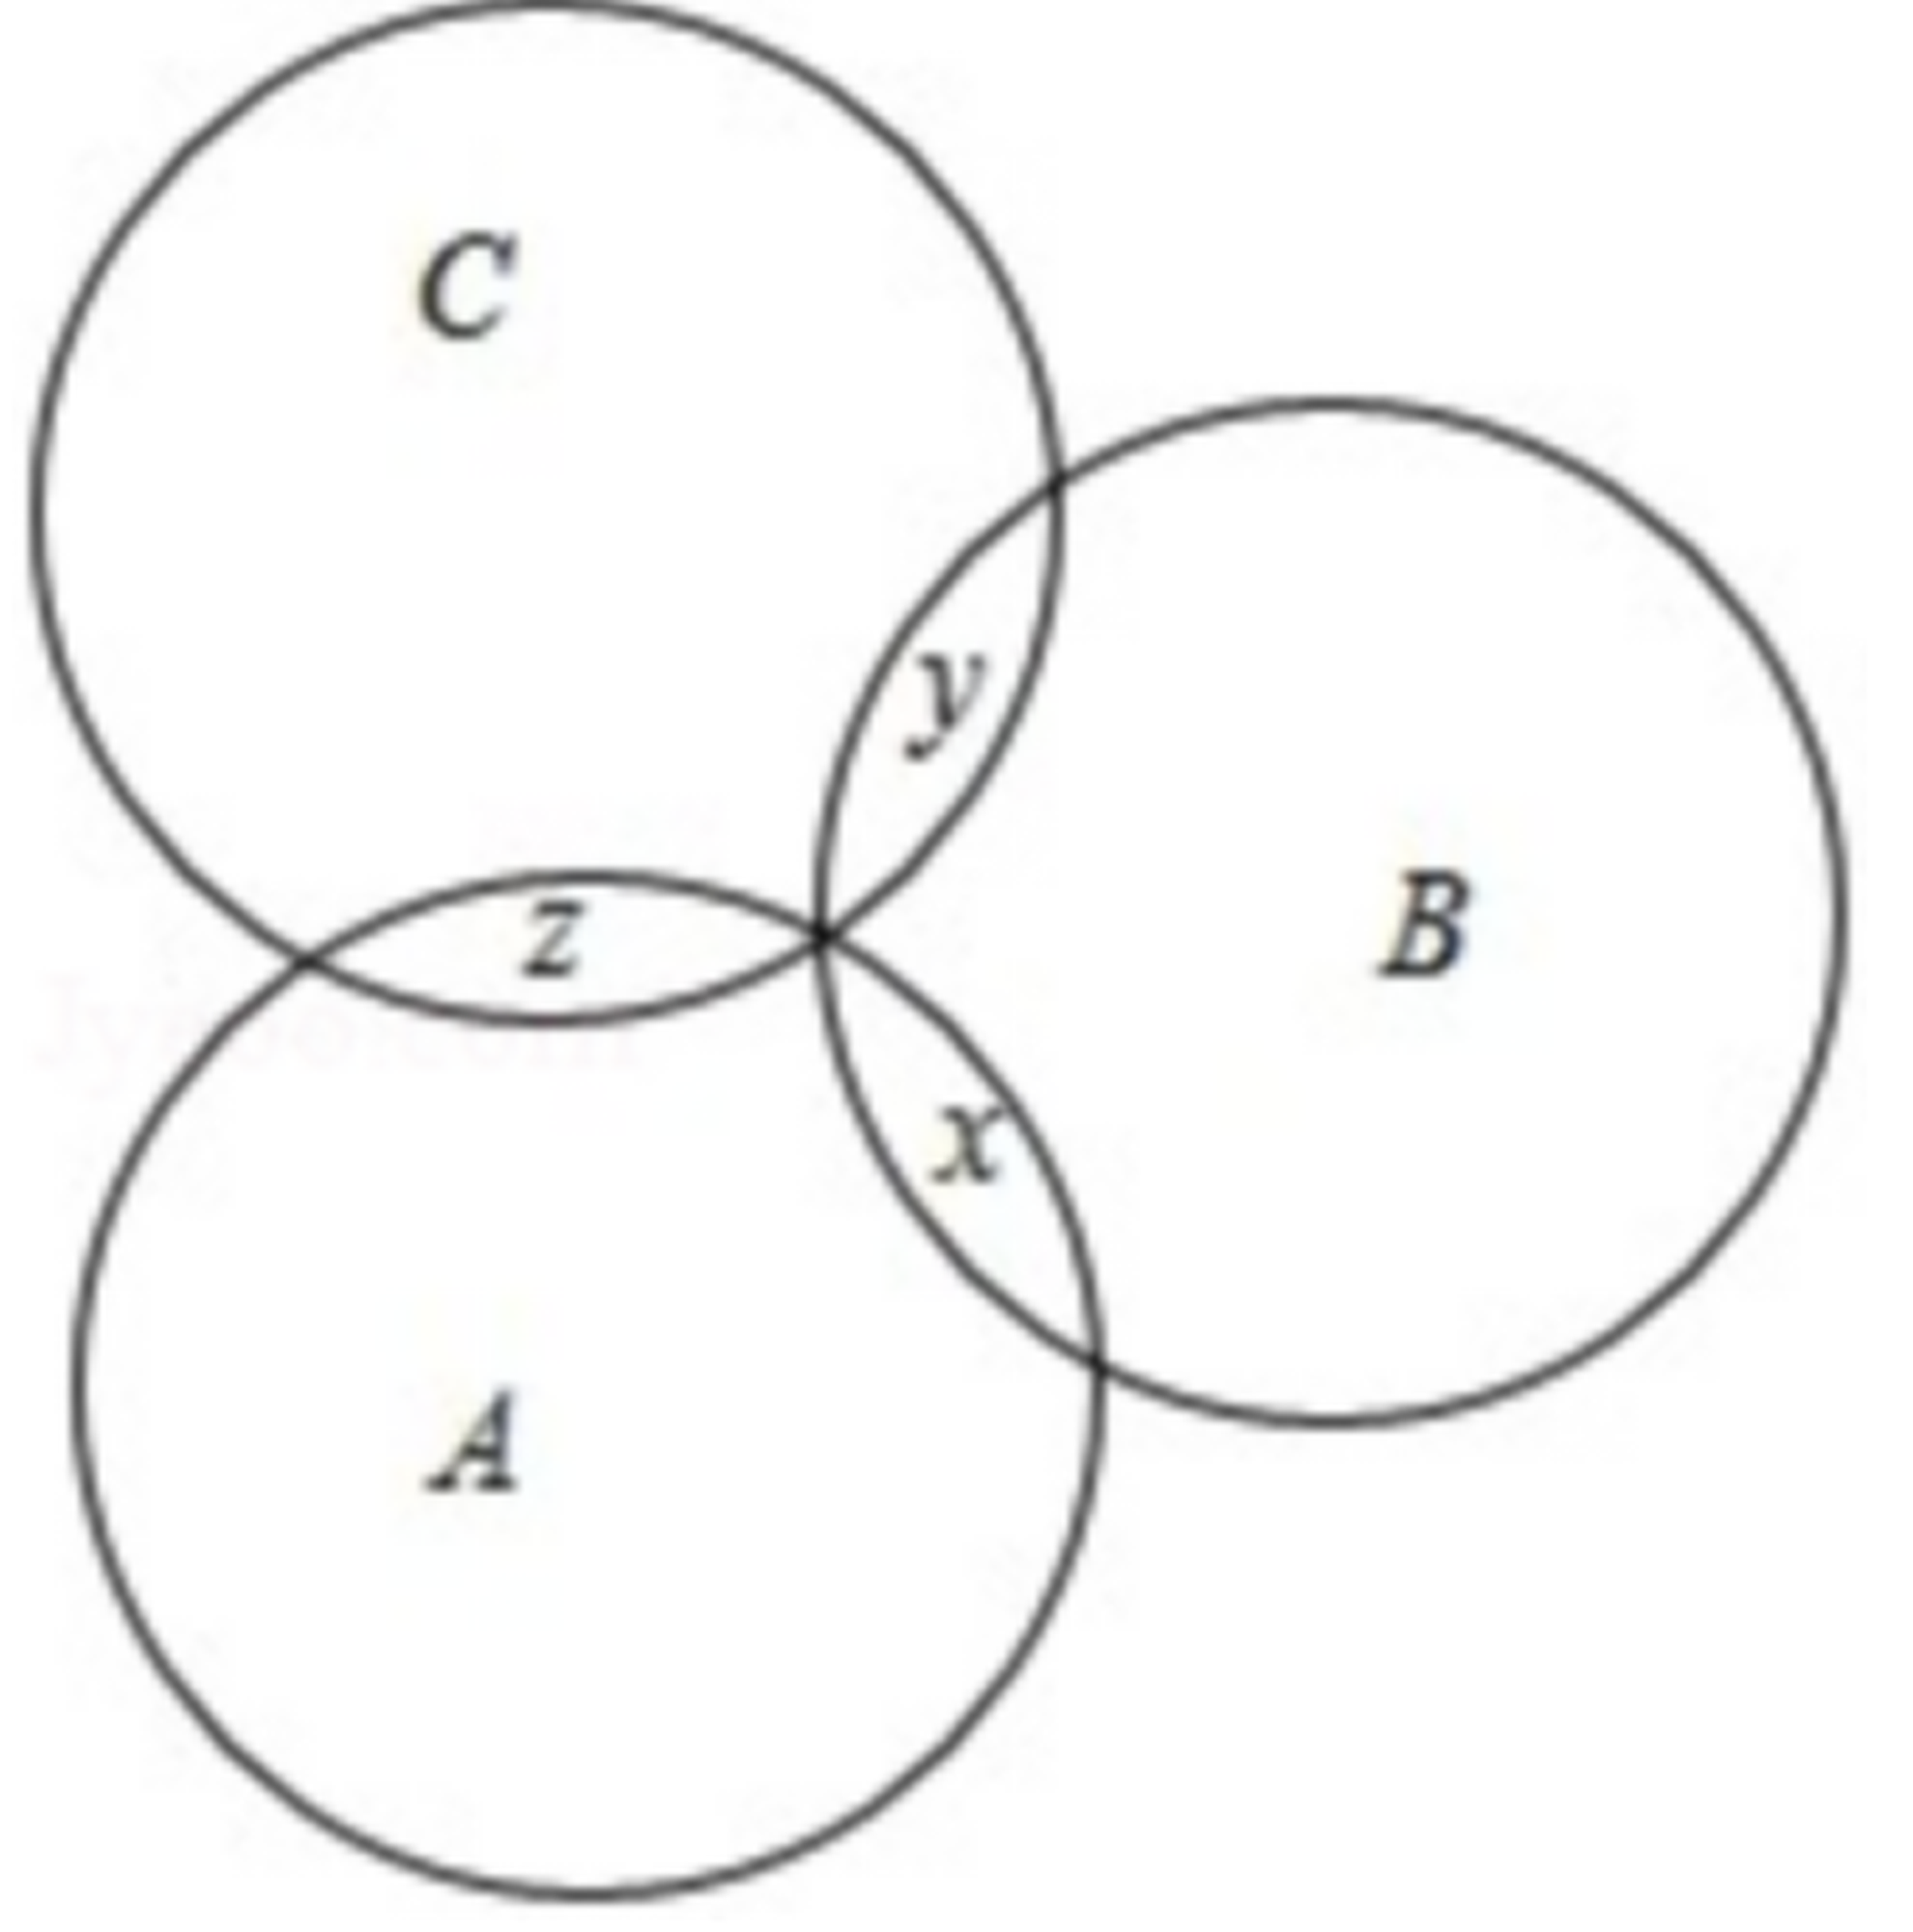
\includegraphics[width=0.30\textwidth]{figures/venn_ABC_x_y_z_h39.png}
\end{center}
\step{因为 $|A\cap B|=|B\cap C|=|C\cap A|=1$，且 $x$、$y$、$z\in\{1,2,3\}$，}
\step{所以集合 $A=\{x,z\}$，$B=\{x,y\}$，$C=\{z,y\}$，}
\step{若 $x=1$，$y=2$，$z=3$，则 $A=\{1,3\}$，$B=\{1,3\}$，$C=\{2,3\}$，}
\step{将 $1$，$2$，$3$ 进行全排列，有 $P_3^3=3\times2=6$ 个.}
\solend

\fi

\item 已知集合 $T=\{1,2,\cdots,2025\}$，对于 $T$ 的每一个非空子集的所有元素，计算它们乘积的倒数，
则所有这样倒数的和为 \blankline[4.4em].

\ans{$2025$}

\ifanswer
\solbegin
\step{集合 $T=\{1,2,\cdots,2025\}$ 的非空子集的个数为 $2^{2025}-1$，}
\step{这些子集中，每个元素的乘积分别为}
\step{$1,2,3,\cdots,2025,1\times2,1\times3,\cdots,1\times2025,\cdots,1\times2\times3\times\cdots\times2025$，}
\step{每项都可以看作是从 $1,2,3,\cdots,2025$ 中选择若干项的乘积，}
\step{$1+\dfrac12+\cdots+\dfrac{1}{2025}+\dfrac{1}{1\times2}+\dfrac{1}{1\times3}+\cdots+\dfrac{1}{2024\times2025}
+\cdots+\dfrac{1}{1\times2\times\cdots\times2025}$}
\step{$=(1+1)\left(1+\dfrac12\right)\cdots\left(1+\dfrac{1}{2025}\right)-1
=2\times\dfrac32\times\dfrac43\times\cdots\times\dfrac{2026}{2025}-1=2025$.}
\solend

\fi

% 第 24 题是压轴题，题干较长；试卷版在它之前量一次页高，尽量不与前文分家（照全稿成例）。
\ansneed{5cm}
% 注：原卷【解析】①③ 两步把 $f(x)$ 印作 $f[x[x]]$，显系笔误，照录未改，见文件头「笔误/存疑」⑦。
\item 若 $X$ 是一个集合，$T$ 是一个以 $X$ 的某些子集为元素的集合，且满足：①$X$ 属于 $T$，
$\varnothing$ 属于 $T$；②$T$ 中任意多个元素的并集属于 $T$；③$T$ 中任意多个元素的交集属于 $T$.
则称 $T$ 是集合 $X$ 上的一个拓扑. 已知函数 $f(x)=[x[x]]$，其中 $[x]$ 表示不大于 $x$ 的最大整数，
当 $x\in(0,n]$，$n\in\N^*$ 时，函数 $f(x)$ 值域为集合 $A_n$，则集合 $A_2$ 上的含有 $4$ 个元素的
拓扑 $T$ 的个数为 \blankline[4.4em].

\ans{$9$}

\ifanswer
\solbegin
\step{由题意，$n=2$，故 $0<x\leqslant2$，}
\step{①当 $0<x<1$ 时，则 $[x]=0$，所以 $f[x[x]]=0$，}
\step{②当 $x=1$ 时，$[x]=1$ 显然 $f(1)=1$，}
\step{③当 $1<x<2$ 时，$[x]=1$，所以 $f[x[x]]=[x]=1$，}
\step{④当 $x=2$ 时，$f(2)=4$，}
\step{所以 $A_2=\{0,1,4\}$，}
\step{因为 $T$ 中含有 $4$ 个元素，其中两个元素 $\varnothing$ 和 $A_2$，}
\step{$A_2=\{0,1,4\}$. 其它两个元素为 $A$、$B$，则
$\begin{cases}A\neq\varnothing\\ A\neq A_2\\ B\neq\varnothing\\ B\neq A_2\\ A\neq B\end{cases}$，}
\step{由对称性，不妨设 $1\leqslant|A|\leqslant|B|\leqslant2$，其中 $|A|$、$|B|$ 表示集合 $A$ 中元素的个数，}
\step{因为 $\begin{cases}A\cap B\in T\\ A\cup B\in T\end{cases}$，又 $|A|\leqslant|B|$，所以 $A\cap B=\varnothing$ 或 $A$，}
\step{若 $A\cap B=\varnothing$，则 $A\cup B$ 只能等于 $A_2$，}
\step{（若 $A\cup B=B$，则 $A\sub B$，则 $A\cap B=A=\varnothing$，矛盾）}
\step{则必有 $\begin{cases}|A|=1\\ |B|=2\end{cases}$，所以 $(A,B)$ 的个数 $\Leftrightarrow$ $A$ 的个数 $=3$ 种，}
\step{即 $\begin{cases}A=\{0\}\\ B=\{1,4\}\end{cases}$ 或 $\begin{cases}A=\{1\}\\ B=\{0,4\}\end{cases}$
或 $\begin{cases}A=\{4\}\\ B=\{0,1\}\end{cases}$；}
\step{若 $A\cap B=A\Leftrightarrow A\sub B$ 此时满足 $A\cup B=B$，}
\step{因为 $A\neq B$ 且 $1\leqslant|A|$ 且 $|B|\leqslant2$，所以 $\begin{cases}|A|=1\\ |B|=2\end{cases}$，}
\step{所以 $B$ 的选择共有 $C_3^2=3$ 种，则 $A$ 的个数有 $C_2^1$ 种，}
\step{所以 $(A,B)$ 的个数 $=2\times3=6$ 种.}
% 这六组「$A$／$B$」按原卷排作两行（前五个一行、第六个另起一行）；因五组并排时
% amsmath 的 cases 会为每组的第二列各留一枚 \quad，本行改排 \left\{\begin{matrix}…\end{matrix}\right.
% 以省下这枚 \quad（照 README「说明」记的高一07 成例），字形与 cases 相同。
\step{（这 $6$ 种是 $\left\{\begin{matrix}A=\{0\}\\ B=\{0,1\}\end{matrix}\right.$、
$\left\{\begin{matrix}A=\{1\}\\ B=\{0,1\}\end{matrix}\right.$、
$\left\{\begin{matrix}A=\{0\}\\ B=\{0,4\}\end{matrix}\right.$、
$\left\{\begin{matrix}A=\{4\}\\ B=\{0,4\}\end{matrix}\right.$、
$\left\{\begin{matrix}A=\{1\}\\ B=\{1,4\}\end{matrix}\right.$、}
\step{$\left\{\begin{matrix}A=\{4\}\\ B=\{1,4\}\end{matrix}\right.$）.}
\step{综上，$T$ 的个数为 $9$ 个.}
\solend

\fi

\end{enumerate}

\end{document}
"
%
% 原始材料是微信公众号图文（公众号「魔都数学加油站」连载「27学年高一 39」，署名「破晓」，
% 2026-09-26 21:29 发布，原文标题「27学年高一39——2026-2027年上海市大同中学高一上周末作业4.1」，
% 原文链接 https://mp.weixin.qq.com/s/HR2hIayXUXNi4zTs3PioiQ ），正文为 11 张 PNG 页。**同一篇里各页分辨率不一致**（2560×3620 与 4762×6735 两档混排：第 1、3、8、10 页为
% 2560×3620，第 2、4、5、6、7、9、11 页为 4762×6735）。原文本身就是一份**讲评版**——除第 15 题
% 外各题题下直接印【解析】（无单独的【答案】行），第 15 题的答案「D」直接印在题干末尾的括号内。
% 试题文字、答案与解析均照原卷录入，未改内容。卷面的粉色斜水印「魔都数学加油站」属水印，未录入。
%
% 卷首标题：原卷页首印作「2026-2027 年大同中学高一上周末作业 4.1」（**卷面标题行即带校名**，
% 年份区间按全稿惯例排 en dash，前缀照原卷保留「年」）。
%
% 篇幅与题号：卷面自「一、填空题」的**第 3 题**起编，终于「附加题」的**第 24 题**，共 22 题
% （填空 3—12、选择 13—16、解答 17—20、附加题 21—24）。第 1、2 题未在该文中发布——这是该
% 公众号连载讲评版的通例（高一02—高一09 等均自第 3 题起编，README「说明」已记），**不是截断**，
% 故本稿题号亦自 3 起。它与 高一40（大同中学 周末作业4.2）同属「周末作业 4」系列但**各自独立起编**
% （4.2 自第 3 题起、终于第 19 题），不是同一份试卷的两半。
%
% 与原卷的排版差异（均已在 README「说明」中交代）：
%   ① 原文自**第 3 题**起（第 1、2 题未在该文中发布），故本稿题号亦自 3 起，填空题以
%      \setcounter{enumi}{2} 起编；选择、解答、附加题三节各按上一节末号另设 \setcounter
%      （选择题 \setcounter{enumi}{12}、解答题 \setcounter{enumi}{16}、附加题 \setcounter{enumi}{20}）；
%   ② 原卷本就印有「一、填空题」「二、选择题」「三、解答题」三节标题，末节印作「附加题」
%      （**不带「四、」**，且题号 21—24 续前编、不另起），本稿照原卷分节，只把标题改排成全稿
%      统一的「大节标题」样式；
%   ③ 原卷是「讲评版」：除第 15 题外，各题题下均印【解析】（**全卷无一条独立的【答案】行**）；
%      第 15 题无解析，答案「D」直接印在题干末尾的括号内。本稿统一改为试卷版隐去、答案版以
%      \ans{}／\ifanswer 块给出，两版彻底分离；原卷写在【解析】末句的结果，本稿照 高一38
%      （同校同系列、同为讲评版）的成例另提为 \ans{}；
%   ④ 数集记号原卷两套并用：实数集作斜体的 $R$（第 7、11、14、17、18、19 题），整数集作斜体
%      $Z$（第 10 题），自然数集作斜体 $N$ 及 $N^*$（第 16、20、21、24 题），本稿按全稿惯例
%      统一写作 $\R$、$\Z$、$\N$、$\N^*$；
%   ⑤ 补集符号原卷两套并用：第 7 题作前缀式的 $C_U$（且题干称全集为 $I$，见「笔误/存疑」①），
%      第 14、15、18 题作上横线（$\overline{H}$、$\overline{A}$、$\overline{B}$），本稿照录、不归一
%      （前缀式写作 $\complement_U$，与 高一c／高一10 的成例一致）；
%   ⑥ 包含符号原卷两套并用：第 3 题作**无下划线**的 $\subset$，第 15、18、20、24 题作**带下划线**
%      的 $\sub$，本稿照录、不归一；
%   ⑦ 原卷填空的横线约两个字宽，本稿按全稿惯例统一排 \blankline[4.4em]；
%   ⑧ 第 7、11、22 题各有插图，取原卷截图、4× LANCZOS 放大（figures/venn_N_cap_CI_M_h39.png、
%      figures/plane_grid_4squares_h39.png、figures/venn_ABC_x_y_z_h39.png）；第 7 题的 Venn 属
%      **题干**（试卷版、答案版都出），第 11、22 题的图在【解析】内（仅答案版出）。第 7 题图
%      左下、第 11 题图的上／左／右边缘带进极淡的原卷粉色水印残影——照全稿「插图直接取自
%      原卷截图、不用 TikZ 重绘、不修图」的体例保留（再裁会切到坐标轴与 $x$、$y$、$O$ 标注）；
%   ⑨ 原卷并列的字母、数字（「$x_1,x_2$」「$a,b$」「$1,2,3,\cdots,11$」）多作半角逗号或不加标点，
%      本稿按全稿惯例改排顿号（$x_1$、$x_2$）或把数列并入行内公式；半角括号、逗号一律排全角，
%      数学式内部的标点照原样；
%   ⑩ 原卷未印副标题，本稿按**本卷实际内容**补出副标题「集合与常用逻辑用语」（依据见下条）。
%
% 副标题（\examtitlest 第二个参数）：本卷卷面未印副标题，由本稿补出，取值按 2026-09-26 起的
%   新口径「只用本卷实际内容的模块名」定为「集合与常用逻辑用语」。依据：全卷 22 题（第 3—24 题）中，
%   第 3、5、7、8、10、11、14、15、16、17、18、19、20、21、22、23、24 题共 17 题是集合的运算与
%   关系、子集／真子集、补集、集合新定义（「全食／偏食」、最小相交、拓扑、特征数）与集合计数，
%   以及命题与常用逻辑用语（第 3 题充要条件、第 5 题存在量词命题、第 17 题命题真假）；其余两题
%   第 4、6 考一元二次方程的根（韦达定理）与方程恒等，第 9、12、13 题是不等式（一元二次不等式组
%   的整数解、一元二次不等式解集、不等式的性质）——不等式合计 3/22，**不足全卷三分之一**，
%   故不并标「不等式」。
%
% 原卷笔误/存疑（均照抄原卷、未改，见源码中该处上方注释）：
%   ① 第 7 题题干称「全集 $I=R$」，而【解析】两处把补集写作 $C_U M$（下标作 $U$），前后记号不一；
%      本稿照录，未改；
%   ② 第 4 题【解析】两处把判别式印作 $\triangle=[2(m-1)^2-16m^2]$（方括号内首项漏了平方，
%      正确应作 $[2(m-1)]^2-16m^2$）；按其所判「$m=\frac12$ 时 $<0$、$m=-\frac12$ 时 $>0$」反推，
%      $[2(m-1)]^2-16m^2$ 在 $m=\frac12$ 时为 $-3<0$、在 $m=-\frac12$ 时为 $5>0$，与结论一致；
%      本稿照录；
%   ③ 第 9 题【解析】把方程组第二式印作 $1-2<-k\leqslant3$，按其结论 $-3\leqslant k<2$ 反推，
%      疑当作 $-2<-k\leqslant3$（原卷多一个「$1$」）；本稿照录；
%   ④ 第 17 题【解析】首句「由数 $y=-x^2+ax-1=-x+3$」中的「由数」显系「由」或「由函数」之误；
%      且末段「若 $p$ 真 $q$ 假…得 $a\in R$」「若 $p$ 假 $q$ 真…此时 $a$ 无解」与结论「$a$ 的取值范围
%      是 $R$」自相矛盾（按 $p:a\leqslant-5$、$q:a>-6$，$p$ 真 $q$ 假应为 $a\leqslant-6$，$p$ 假 $q$ 真
%      应为 $a>-5$，合起来是 $a\leqslant-6$ 或 $a>-5$，并非 $R$）；本稿一律照录，未按正确解法改写；
%   ⑤ 第 18 题【解析】(2) 把 $B=\{x\mid x^2+a\leqslant0\}$（$a<0$）印作右端开的
%      $\{x\mid-\sqrt{-a}\leqslant x<\sqrt{-a}\}$（应为闭的「$\leqslant$」）；按其所判
%      $\sqrt{-a}<\frac12$ 反推，不影响结论；本稿照录；
%   ⑥ 第 22 题【解析】在 $x=1$、$y=2$、$z=3$ 时把 $B=\{x,y\}$ 印作 $\{1,3\}$（应为 $\{1,2\}$），
%      与本行前面「$B=\{x,y\}$」不合；本稿照录；
%   ⑦ 第 24 题【解析】①③ 两步把 $f(x)$ 印作 $f[x[x]]$，显系笔误；本稿照录。
%   ⑧ 第 8 题【解析】「即方程 $x^2+ax+b=x$，$x^2+(a-1)x+b=0$ **由**两个相等的实数根为 $4$」——
%      「由」当为「有」（「设…是…有」的杂糅）；本稿照录；
%   ⑨ 第 10 题：题设 $a\oplus b=b(a^2+b^2+1)$，而集合定义里含 $\dfrac{a\oplus b}{2b}$；$-2<a<b<2$、
%      $a$、$b\in\Z$ 时 $(a,b)=(-1,0)$ 也合条件、却使分母 $2b=0$，原卷解析仍代入该组并约去
%      $b$ 得 $x=1$（答案集恰好不变）；本稿照录；
%   ⑩ 第 15 题选项列里 ② 与 ③ 之间**漏排分隔号**（原卷作「② $\overline{A}\cap B=\varnothing$③
%      $\overline{A}\sub\overline{B}$；」——①、③ 后都有「；」，② 后没有）；本稿照录；
%   ⑪ 第 20(2) 把 $\{1,2,\cdots,20\}$ 分成的 11 个集合里，$\{8,11\}$ 与 $\{9,12\}$ 之间误用
%      **句号**「.」（同行其余处皆逗号）；本稿照录；
%   ⑫ 第 20(3)① 推理不严：原卷写「选 5 则不选 1、9；选 6 则不选 2、10；选 7 则不选 3、11；
%      则只剩 4、8」——但 4 与 8 相差 $4$、不能同选，该情形实际最多只能取 $4$ 个；末句结论
%      「不超过 $5$ 个」仍成立；本稿照录；
%   ⑬ 第 16 题【解析】两种下标并存：「所以在 $A_i$ 的特征数构成中」原卷作斜体 $A_i$，而
%      「要使 $X_1+X_2+X_3$ 最大（小），则（应）在集合 $A_1$ 中首先放置…」两处原卷作
%      **数字 $1$**（与同句 $X_1$ 的角标同形）；本稿照录、未归一。
%
% 图取原卷截图（依次见各处的 \includegraphics 前的注释），4× LANCZOS 放大。
\documentclass[a4paper,11pt]{article}
\usepackage{common}

\begin{document}

\examtitlest[3]{2026--2027 年大同中学高一上周末作业 4.1}{集合与常用逻辑用语}

\bigsec{一、填空题}

\begin{enumerate}
\setcounter{enumi}{2}

\item “$x\geqslant a$”是“$0<x<2$”的必要非充分条件，则实数 $a$ 的取值范围是 \blankline[4.4em].

\ans{$(-\infty,0]$}

\ifanswer
\solbegin
\step{因为 $x\geqslant a$ 是 $0<x<2$ 的必要非充分条件，所以 $(0,2)\subset[a,+\infty)$，所以 $a\leqslant0$，}
\step{则实数 $a$ 的取值范围是 $(-\infty,0]$.}
\solend

\fi

% 注：原卷$[2(m-1)^2-16m^2]$ 首项漏了平方（应为 $[2(m-1)]^2-16m^2$），照录未改，见文件头「笔误/存疑」②。
\item 若关于 $x$ 的方程 $x^2+2(m-1)x+4m^2=0$ 有两个实数根，且这两根互为倒数，则 $m=$ \blankline[4.4em].

\ans{$-\dfrac12$}

\ifanswer
\solbegin
\step{设 $x_1$、$x_2$ 是方程 $x^2+2(m-1)x+4m^2=0$ 有两个实数根，}
\step{则 $x_1x_2=4m^2=1$，解得 $m=\dfrac12$ 或 $m=-\dfrac12$，}
\step{又当 $m=\dfrac12$ 时，$\triangle=[2(m-1)^2-16m^2]<0$，舍去，}
\step{当 $m=-\dfrac12$ 时，$\triangle=[2(m-1)^2-16m^2]>0$，故 $m=-\dfrac12$.}
\solend

\fi

\item 已知命题：“存在 $x\in[1,2]$，使 $x^2+2x+a\geqslant0$”为真命题，则 $a$ 的取值范围是 \blankline[4.4em].

\ans{$a\geqslant-8$}

\ifanswer
\solbegin
\step{若存在 $x\in[1,2]$，使 $x^2+2x+a\geqslant0$，}
\step{则等价为存在 $x\in[1,2]$，使 $x^2+2x\geqslant-a$，}
\step{当存在 $x\in[1,2]$ 时，设 $y=x^2+2x=(x+1)^2-1$，则 $3\leqslant y\leqslant8$，}
\step{所以要使 $x^2+2x\geqslant-a$，则 $8\geqslant-a$，即 $a\geqslant-8$.}
\solend

\fi

\item 已知方程 $a(3x+2)+b(2x-3)=8x+3$ 有无穷多个解，则 $a:b=$ \blankline[4.4em].

\ans{$30:7$}

\ifanswer
\solbegin
\step{$a(3x+2)+b(2x-3)=(3a+2b)x+2a-3b=8x+3$ 有无穷多个解，}
\step{所以 $\begin{cases}3a+2b=8\\ 2a-3b=3\end{cases}$，解得 $a=\dfrac{30}{13}$，$b=\dfrac{7}{13}$，所以 $a:b=30:7$.}
\solend

\fi

% 注：原卷题干称「全集 $I=R$」，而【解析】两处把补集写作 $C_U M$（下标作 $U$），前后记号不一；
%     照录未改，见文件头「笔误/存疑」①。
\item 已知集合 $M=\{x\mid y=\sqrt{3-x^2}\}$，$N=\{x\mid-3\leqslant x\leqslant1\}$，全集 $I=\R$，
则图中阴影部分表示的集合为 \blankline[4.4em].

% 图取原卷截图（01.png，2560×3620）右栏，4× LANCZOS 放大。
\begin{center}
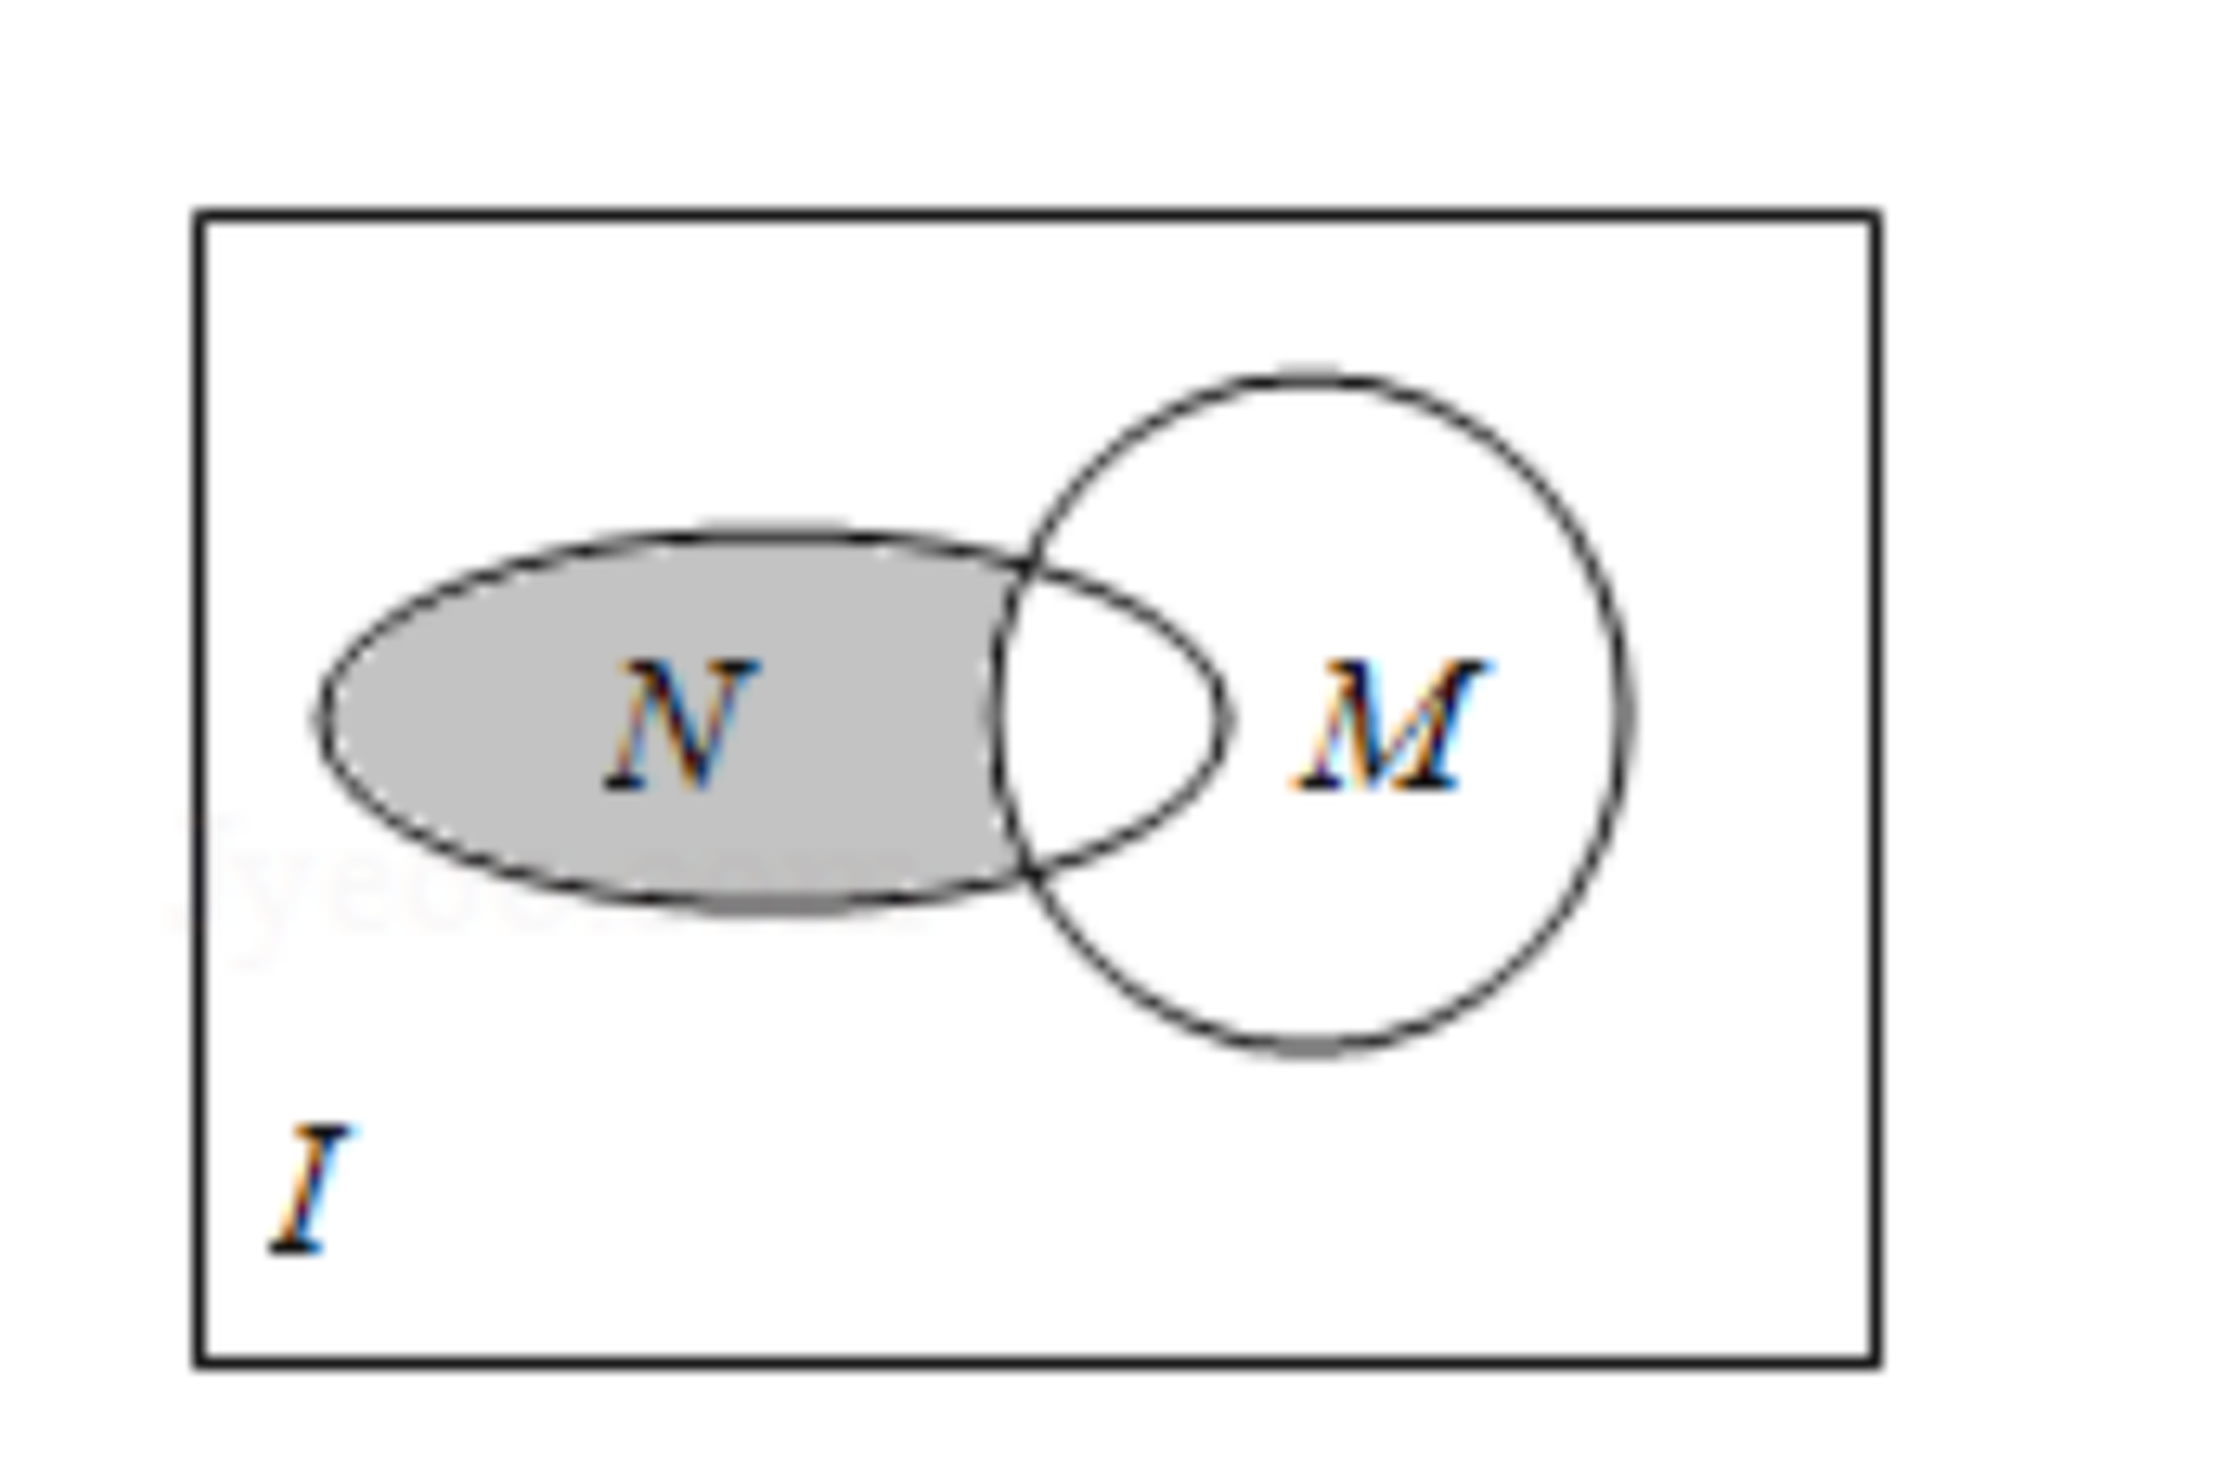
\includegraphics[width=0.30\textwidth]{figures/venn_N_cap_CI_M_h39.png}
\end{center}

\ans{$[-3,-\sqrt3)$}

\ifanswer
\solbegin
\step{阴影部分用集合表示为 $N\cap(\complement_UM)$.}
\step{则 $M=\{x\mid y=\sqrt{3-x^2}\}=\{x\mid3-x^2\geqslant0\}=\{x\mid-\sqrt3\leqslant x\leqslant\sqrt3\}$，}
\step{则 $\complement_UM=\{x\mid x>\sqrt3\text{ 或 }x<-\sqrt3\}$，$N=\{x\mid|x+1|\leqslant2\}=\{x\mid-3\leqslant x\leqslant1\}$，}
\step{则 $N\cap(\complement_UM)=\{x\mid-3\leqslant x<-\sqrt3\}$.}
\solend

\fi

\item 已知 $f(x)=x^2+ax+b$，集合 $\{x\mid f(x)=x\}=\{4\}$，将集合 $M=\{x\mid f(x)=4\}$ 用列举法表示 \blankline[4.4em].

\ans{$\{3,4\}$}

\ifanswer
\solbegin
\step{已知 $f(x)=x^2+ax+b$，集合 $\{x\mid f(x)=x\}=\{4\}$，}
% 注：原卷本行作「…$x^2+(a-1)x+b=0$ **由**两个相等的实数根为 $4$」——「由」当为「有」
%     （「设…是…有」的杂糅）；本稿照录未改，见文件头「原卷笔误/存疑」⑧。
\step{即方程 $x^2+ax+b=x$，$x^2+(a-1)x+b=0$ 由两个相等的实数根为 $4$，}
\step{所以 $\triangle=(a-1)^2-4b=0$，即 $x^2+(a-1)x+b=(x-4)^2$，所以 $b=16$，$a=-7$，}
\step{所以 $f(x)=x^2+ax+b=x^2-7x+16$，所以集合 $M=\{x\mid f(x)=4\}$，}
\step{即 $x^2-7x+16=4$，$x^2-7x+12=0$，故 $M=\{x\mid f(x)=4\}=\{3,4\}$.}
\solend

\fi

% 注：原卷方程组第二式印作 $1-2<-k\leqslant3$，按其结论 $-3\leqslant k<2$ 反推疑当作 $-2<-k\leqslant3$，
%     照录未改，见文件头「笔误/存疑」③。
\item 关于 $x$ 的不等式组 $\begin{cases}x^2-x-2>0\\ 2x^2+(2k+5)x+5k<0\end{cases}$ 的整数解的集合为 $\{-2\}$，
则实数 $k$ 的取值范围 \blankline[4.4em].

\ans{$-3\leqslant k<2$}

\ifanswer
\solbegin
\step{原不等式组即 $\begin{cases}(x-2)(x+1)>0\\ (x+k)(2x+5)<0\end{cases}$，整数解的集合为 $A$，若 $A=\{-2\}$，}
\step{则 $(-2+k)(2\times(-2)+5)<0$，所以 $k<2$，且有 $\begin{cases}-k>-\dfrac52\\ 1-2<-k\leqslant3\end{cases}$，}
\step{解得 $-3\leqslant k<2$.}
\solend

\fi

\item 规定 $\oplus$ 与 $\otimes$ 是两个运算符号，其运算法则如下，对任意实数 $a$、$b$ 有：$a\otimes b=ab$，
$a\oplus b=b(a^2+b^2+1)$. 若 $-2<a<b<2$ 且 $a$、$b\in\Z$，
$A=\left\{x\mid x=2(a\otimes b)+\dfrac{a\oplus b}{2b}\right\}$，则用列举法表示集合 $A=$ \blankline[4.4em].

\ans{$\left\{1,-\dfrac12\right\}$}

\ifanswer
\solbegin
\step{$A=\left\{x\mid x=2(a\otimes b)+\dfrac{a\oplus b}{2b}\right\}
=\left\{x\mid x=2ab+\dfrac{b(a^2+b^2+1)}{2b}\right\}$}
\step{$=\left\{x\mid x=2ab+\dfrac12a^2+\dfrac12b^2+\dfrac12\right\}
=\left\{x\mid x=\dfrac12(a+b)^2+ab+\dfrac12\right\}$，}
% 注：题设含 $\dfrac{a\oplus b}{2b}$，而 $-2<a<b<2$、$a$、$b\in\Z$ 时 $(a,b)=(-1,0)$ 也合条件、
%     却使分母 $2b=0$；原卷解析仍代入该组并约去 $b$ 得 $x=1$（答案集恰好不变）。本稿照录，
%     见文件头「原卷笔误/存疑」⑨。
\step{当 $a=-1$，$b=0$ 时，$x=1$；当 $a=-1$，$b=1$ 时，$x=-\dfrac12$；}
\step{当 $a=0$，$b=1$ 时，$x=1$；所以 $A=\left\{1,-\dfrac12\right\}$.}
\solend

\fi

\item 高斯是德国著名的数学家，近代数学奠基者之一，享有“数学王子”的称号，为了纪念数学家高斯，
我们把取整函数 $y=[x]$，$x\in\R$ 称为高斯函数，其中 $[x]$ 表示不超过 $x$ 的最大整数，
如 $[1.1]=1$，$[-1.1]=-2$. 则点集 $P=\{(x,y)\mid[x]^2+[y]^2=1\}$
所表示的平面区域的面积是 \blankline[4.4em].

\ans{$4$}

\ifanswer
\solbegin
\step{$[x]^2+[y]^2=1$ 由 $\begin{cases}[x]=0\\ [y]=-1\end{cases}$ 或 $\begin{cases}[x]=0\\ [y]=1\end{cases}$
或 $\begin{cases}[x]=-1\\ [y]=0\end{cases}$ 或 $\begin{cases}[x]=1\\ [y]=0\end{cases}$ 四个平面区域组成，}
\step{即 $\begin{cases}0\leqslant x<1\\ -1\leqslant y<0\end{cases}$ 或 $\begin{cases}0\leqslant x<1\\ 1\leqslant y<2\end{cases}$
或 $\begin{cases}-1\leqslant x<0\\ 0\leqslant y<1\end{cases}$ 或 $\begin{cases}1\leqslant x<2\\ 0\leqslant y<1\end{cases}$，}
\step{作出平面区域如图所示，平面区域由四个边长为 $1$ 的正方形组成，}
% 图在【解析】内（仅答案版出），取原卷截图（03.png，2560×3620）中部，4× LANCZOS 放大。
\begin{center}
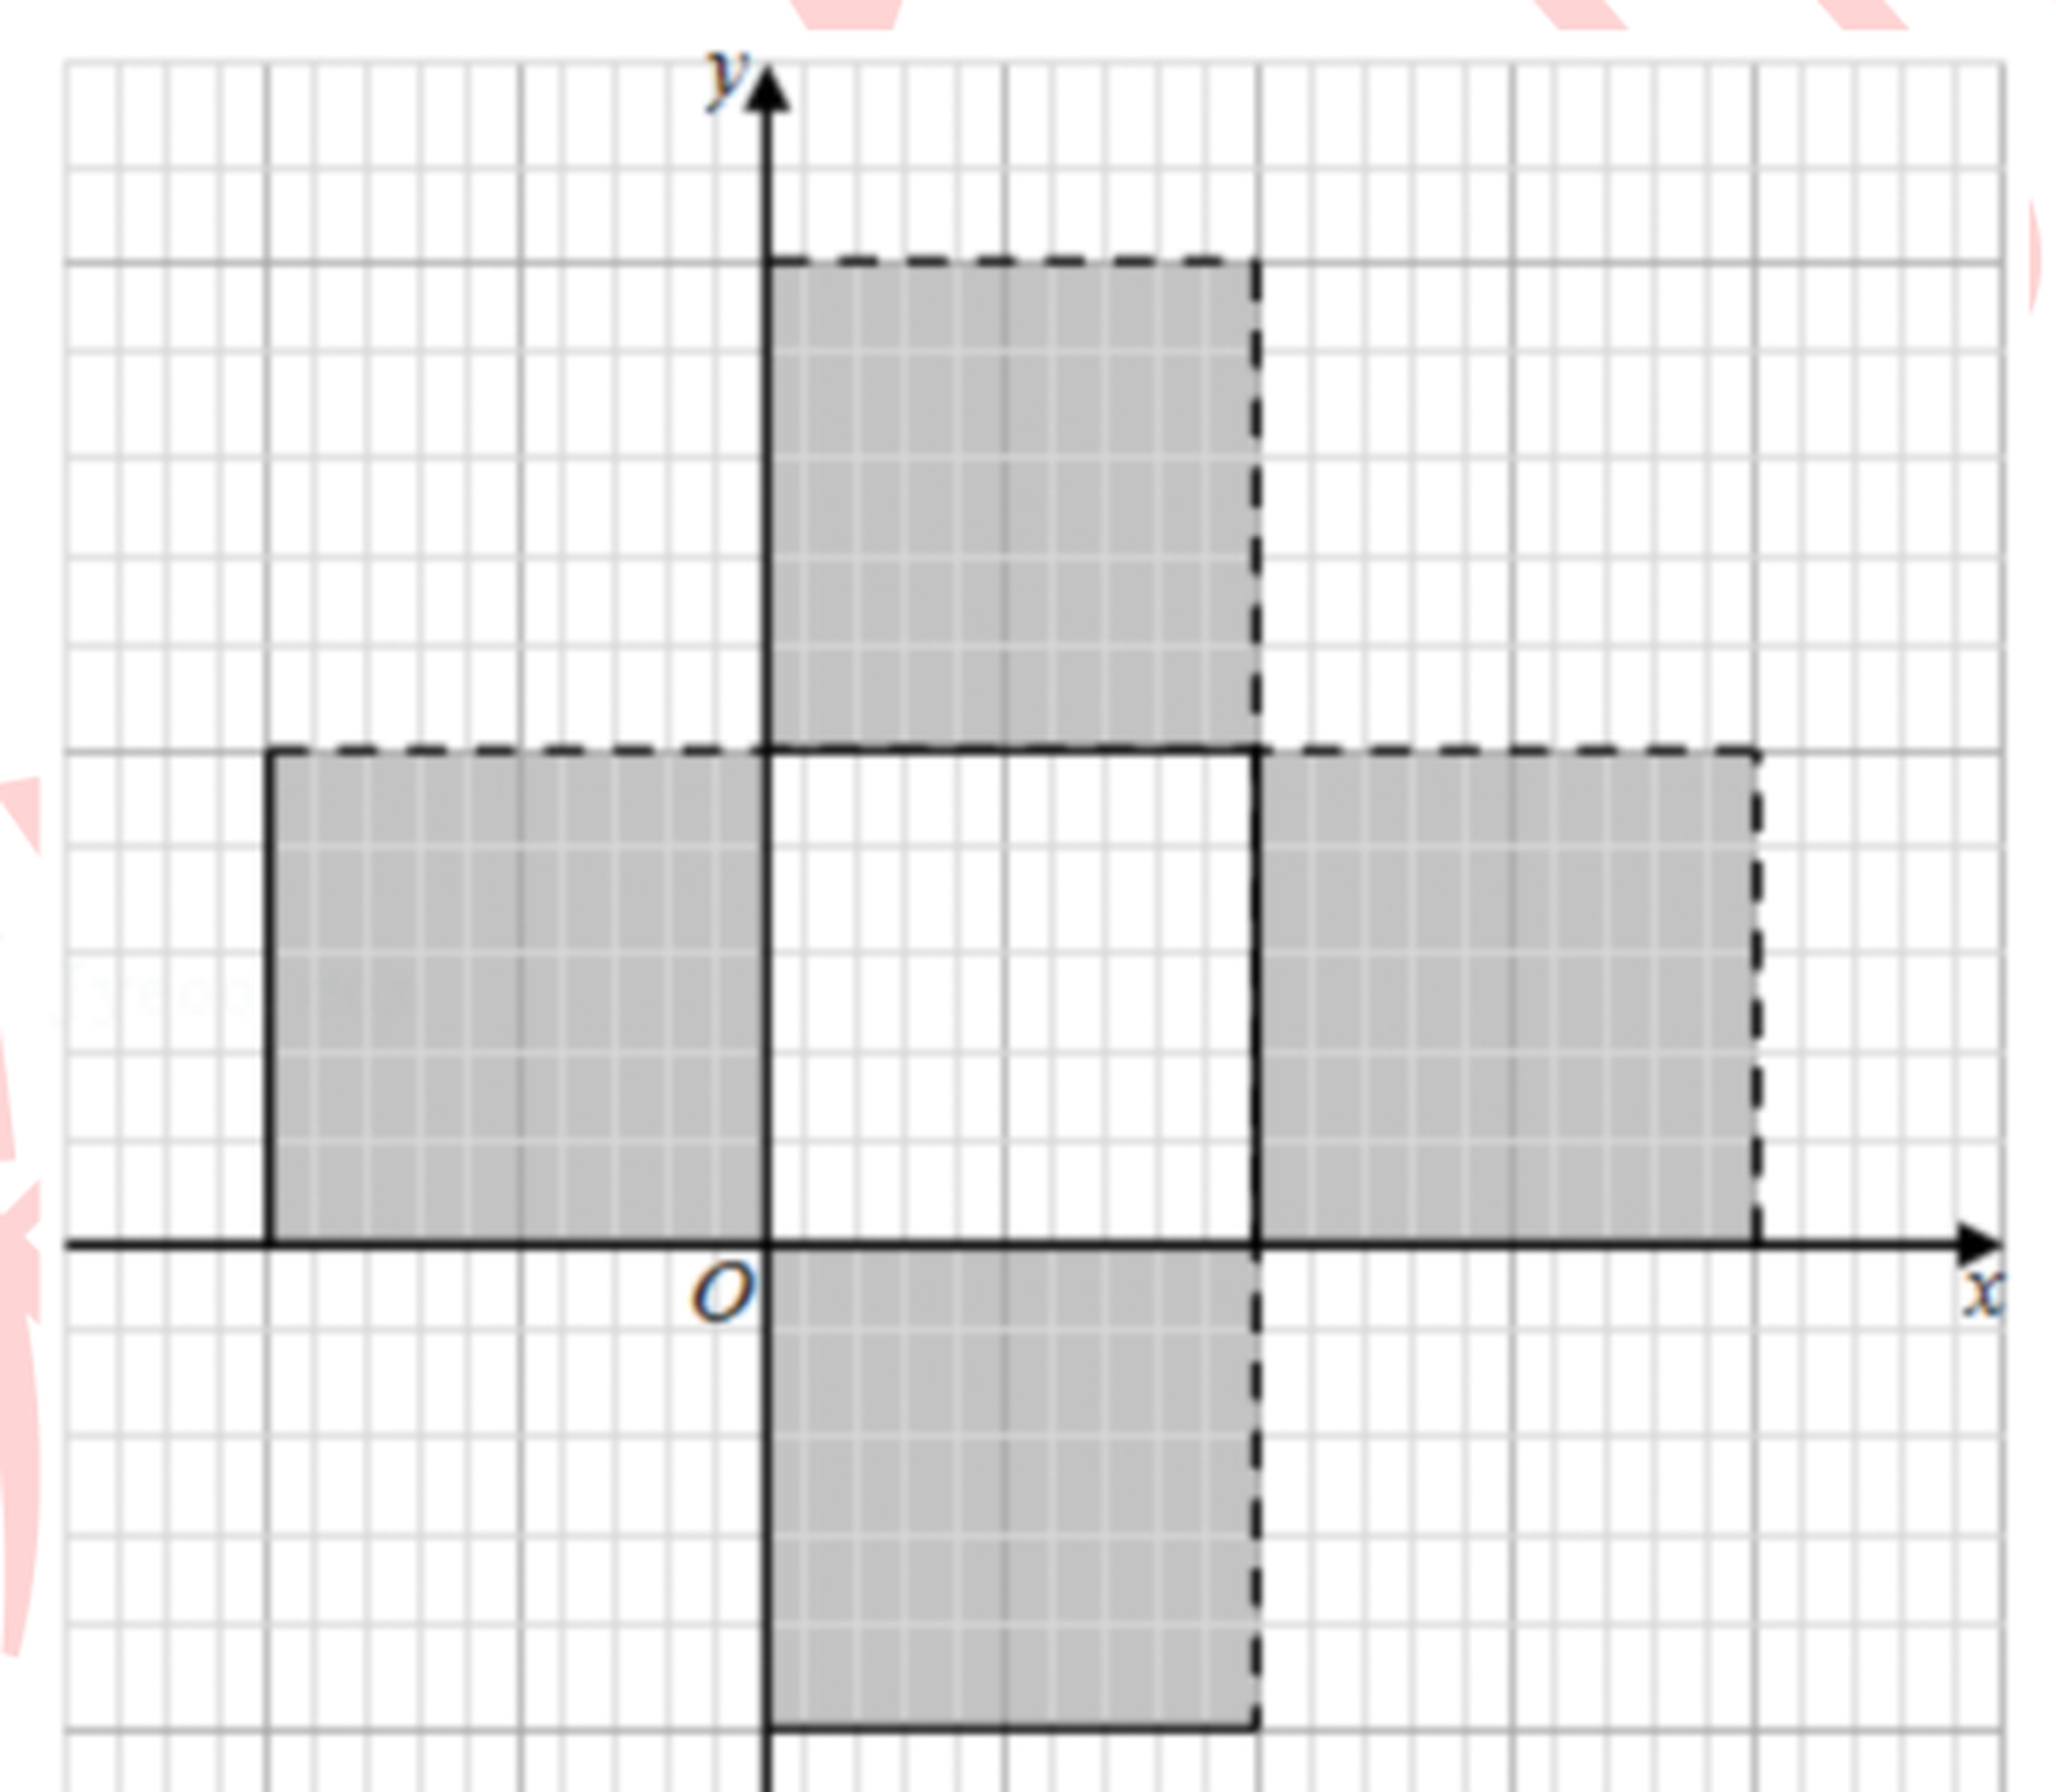
\includegraphics[width=0.38\textwidth]{figures/plane_grid_4squares_h39.png}
\end{center}
\step{总面积为 $1\times4=4$.}
\solend

\fi

\item 关于 $x$ 的不等式 $ax^2+bx+c>0$ 的解集为 $\{x\mid x<\beta\text{ 或 }x>\gamma\}(0<\beta<\gamma)$，
则不等式 $a(x^2+1)+b(x-1)+c>2ax$ 的解集为 \blankline[4.4em].

\ans{$(-\infty,\beta+1)\cup(\gamma+1,+\infty)$}

\ifanswer
\solbegin
\step{由题意得 $\beta$、$\gamma$ 为方程 $ax^2+bx+c=0$ 的两根且 $a>0$，}
\step{则 $\beta+\gamma=-\dfrac ba$，$\beta\gamma=\dfrac ca$，故 $b=-a(\beta+\gamma)$，$c=\beta\gamma a$，}
\step{则不等式可化为 $a(x^2+1)-a(\beta+\gamma)(x-1)+\beta\gamma a>2ax$，}
\step{因为 $a>0$，所以 $x^2+1-(\beta+\gamma)(x-1)+\beta\gamma>2x$，}
\step{即 $x^2-(\beta+\gamma+2)x+(\beta+\gamma+\beta\gamma+1)>0$，所以 $(x-\beta-1)(x-\gamma-1)>0$，}
\step{解得 $x<\beta+1$ 或 $x>\gamma+1$，所以不等式解集为 $(-\infty,\beta+1)\cup(\gamma+1,+\infty)$.}
\solend

\fi

\end{enumerate}

\bigsec{二、选择题}

\begin{enumerate}
\setcounter{enumi}{12}

\item 设 $a<b<0$，则下列不等式中不成立的是\mbox{（\quad）}

\keepwithprev
A. $\dfrac1a>\dfrac1b$\qquad B. $\dfrac{1}{a-b}>\dfrac1a$\qquad C. $|a|>-b$\qquad D. $\sqrt{-a}>\sqrt{-b}$

\ans{$B$}

\ifanswer
\solbegin
\step{令 $a=-2$，$b=-1$，}
\step{A、$-\dfrac12>-1$，正确；B、$-1<-\dfrac12$，故 B 错误；C、$2>1$，正确；}
\step{D、$\sqrt2>1$，正确；故选 B.}
\solend

\fi

\item 设实数集 $\R$ 为全集，集合 $P=\{x\mid f(x)=0\}$，$Q=\{x\mid g(x)=0\}$，$H=\{x\mid h(x)=0\}$，
则方程 $\dfrac{f^2(x)+g^2(x)}{h(x)}=0$ 的解集是\mbox{（\quad）}

\keepwithprev
A. $P\cap Q\cap\overline{H}$\qquad B. $P\cap Q$\qquad C. $P\cap Q\cap H$\qquad D. $P\cap Q\cup H$

\ans{$A$}

\ifanswer
\solbegin
\step{方程 $\dfrac{f^2(x)+g^2(x)}{h(x)}=0$ 等价于 $\begin{cases}f(x)=0\\ g(x)=0\\ h(x)\neq0\end{cases}$，}
\step{又因为 $P=\{x\mid f(x)=0\}$，$Q=\{x\mid g(x)=0\}$，$H=\{x\mid h(x)=0\}$，}
\step{所以方程 $\dfrac{f^2(x)+g^2(x)}{h(x)}=0$ 的解集是 $P\cap Q\cap\overline{H}$，故选 A.}
\solend

\fi

\item 设全集 $U$，在下列条件中，是 $B\sub A$ 的充要条件的有\mbox{（\quad）}

\keepwithprev
% 注：原卷此行 ② 与 ③ 之间**漏排分隔号**（①、③ 后都有「；」，② 后没有）；
%     本稿照录未补，见文件头「原卷笔误/存疑」⑩。
①$A\cup B=A$；\qquad ②$\overline{A}\cap B=\varnothing$\qquad ③$\overline{A}\sub\overline{B}$；\qquad ④$A\cup\overline{B}=U$

\keepwithprev
A. $1$ 个\qquad B. $2$ 个\qquad C. $3$ 个\qquad D. $4$ 个

\ans{$D$}

\item 已知集合 $M=\{x\mid x\in\N,0<x\leqslant15\}$，$A_1$、$A_2$、$A_3$ 满足：①$A_1\cup A_2\cup A_3=M$；
②每个集合都恰有 $5$ 个元素. 集合 $A_i(i=1,2,3)$ 中最大元素与最小元素之和称为 $A_i$ 的特征数，
记为 $X_i(i=1,2,3)$，则 $X_1+X_2+X_3$ 的值不可能为\mbox{（\quad）}

\keepwithprev
A. $37$\qquad B. $39$\qquad C. $48$\qquad D. $57$

\ans{$A$}

\ifanswer
\solbegin
\step{因为集合 $M=\{x\mid x\in\N,0<x\leqslant15\}=\{1,2,3,\cdots,15\}$，}
\step{又因为集合 $A_1$、$A_2$、$A_3$ 中，每个集合恰有 $5$ 个元素，}
\step{且 $A_1\cup A_2\cup A_3=M$ 有 $15$ 个元素，所以集合 $A_1$、$A_2$、$A_3$ 中没有重复元素，}
\step{因为 $1$ 是集合 $M$ 中数值最小的元素，$15$ 是集合 $M$ 中数值最大的元素，}
\step{所以在 $A_i$ 的特征数构成中，必有 $1$ 和 $15$，不妨设 $1\in A_1$，$15\in A_1$，}
% 注：原卷本行（与下面「最小」那句）在「集合」后的角标是**数字 $1$**（同句 $X_1$ 的角标同形），
%     而非上一行「$A_i$ 的特征数构成」里的斜体 $A_i$——原卷两种下标并存，本稿照录、不归一，
%     见文件头「原卷笔误/存疑」⑬。
\step{要使 $X_1+X_2+X_3$ 最大，则应该在集合 $A_1$ 中首先放置数值较小的元素，}
\step{即 $A_1=\{1,2,3,4,15\}$，所以 $5$ 与 $14$ 是剩下元素中数值最小或最大的元素，}
\step{同理，不妨设 $5\in A_2$，$14\in A_2$，接着在 $A_2$ 中再次放置数值较小的元素，}
\step{即 $A_2=\{5,6,7,8,14\}$，则 $A_3=\{9,10,11,12,13\}$，}
\step{此时 $X_1+X_2+X_3$ 有最大值为 $1+15+5+14+9+13=57$，}
\step{即 $X_1+X_2+X_3\leqslant57$；}
% 注：同上一处——原卷此行角标是**数字 $1$**（$A_1$），本稿照录，未与「$A_i$」归一。
\step{要使 $X_1+X_2+X_3$ 最小，则在集合 $A_1$ 中首先放置数值较大的元素，}
\step{即 $A_1=\{1,12,13,14,15\}$，所以 $2$ 与 $11$ 是剩下元素中数值最小或最大的元素，}
\step{同理，不妨设 $2\in A_2$，$11\in A_2$，接着在 $A_2$ 中再次放置数值较大的元素，}
\step{即 $A_2=\{2,8,9,10,11\}$，则 $A_3=\{3,4,5,6,7\}$，}
\step{此时 $X_1+X_2+X_3$ 有最小值为 $1+15+2+11+3+7=39$，}
\step{即 $X_1+X_2+X_3\geqslant39$，}
\step{综上，$39\leqslant X_1+X_2+X_3\leqslant57$，故选 A.}
\solend

\fi

\end{enumerate}

\bigsec{三、解答题}

\begin{enumerate}
\setcounter{enumi}{16}

% 注：原卷首句「由数 $y=-x^2+ax-1=-x+3$」中的「由数」显系「由」或「由函数」之误；末段
%     的两处分类讨论与结论自相矛盾（详见文件头「笔误/存疑」④）。本稿一律照录，未改。
\item 命题 $p$：函数 $y=-x^2+ax-1$ 与 $y=-x+3$ 图象交点的横坐标均为负值，
命题 $q$：关于 $x$ 的方程 $2(1-x)a+(x^2-10x-3)=0$ 的两个根，一个大于 $3$，另一个小于 $3$；
若命题 $p$ 和命题 $q$ 中有且仅有一个是真命题，求 $a$ 的取值范围.

\ans{$\R$}

\ifanswer
\solbegin
\step{由数 $y=-x^2+ax-1=-x+3$ 得 $x^2-(a+1)x+4=0$，}
\step{若横坐标均为负值，则满足 $\begin{cases}\Delta=(a+1)^2-16\geqslant0\\ x_1x_2=4>0\\ x_1+x_2=a+1<0\end{cases}$
得 $\begin{cases}a\geqslant3\text{ 或 }a\leqslant-5\\ a<-1\end{cases}$，得 $a\leqslant-5$，}
\step{即 $p:a\leqslant-5$，}
\step{若方程 $2(1-x)a+(x^2-10x-3)=0$ 的两个根，一个大于 $3$，另一个小于 $3$；}
\step{设 $f(x)=2(1-x)a+(x^2-10x-3)$，则 $f(3)<0$，即 $-4a-24<0$，}
\step{得 $a>-6$，即 $q:a>-6$，}
\step{因为命题 $p$ 和命题 $q$ 中有且仅有一个是真命题，}
\step{若 $p$ 真 $q$ 假，则 $\begin{cases}a\leqslant-5\\ a>-6\end{cases}$，得 $a\in\R$，}
\step{若 $p$ 假 $q$ 真，则 $\begin{cases}a>-5\\ a\leqslant-6\end{cases}$，此时 $a$ 无解，}
\step{综上，实数 $a$ 的取值范围是 $\R$.}
\solend

\fi

\ansspace[8]

\item 设全集是实数集 $\R$，$A=\left\{x\mid\dfrac{1-2x}{x-3}\geqslant0\right\}$，$B=\{x\mid x^2+a\leqslant0\}$.

\begin{enumerate}[label=(\arabic*)]

\item 当 $a=-4$ 时，求 $A\cup B$；

\item 若 $\overline{A}\cap B=B$，求实数 $a$ 的取值范围.

\end{enumerate}

\ans{（1）$\{x\mid-2\leqslant x<3\}$；（2）$\left(-\dfrac14,+\infty\right)$}

\ifanswer
\solbegin
\stepm{(1)}{$A=\left\{x\mid\dfrac{1-2x}{x-3}\geqslant0\right\}=\left\{x\mid\dfrac12\leqslant x<3\right\}$，$B=\{x\mid x^2+a\leqslant0\}$.}
\step{当 $a=-4$ 时，$B=\{x\mid-2\leqslant x\leqslant2\}$，所以 $A\cup B=\{x\mid-2\leqslant x<3\}$.}
\stepm{(2)}{$\overline{A}=\left\{x\mid x\geqslant3\text{ 或 }x<\dfrac12\right\}$，$B=\{x\mid x^2+a\leqslant0\}$.}
\step{由 $\overline{A}\cap B=B$，得 $B\sub\overline{A}$，}
\step{则当 $a>0$ 时，$B=\varnothing$，满足 $B\sub\overline{A}$，则 $a>0$ 成立，}
\step{则当 $a=0$ 时，$B=\{0\}$，满足 $B\sub\overline{A}$，则 $a=0$ 成立，}
\step{当 $a<0$ 时，$B=\{x\mid-\sqrt{-a}\leqslant x<\sqrt{-a}\}$，}
\step{得 $\sqrt{-a}<\dfrac12$，即 $-\dfrac14<a<0$，}
\step{综上，实数 $a$ 的取值范围是 $\left(-\dfrac14,+\infty\right)$.}
\solend

\fi

\ansspace[6]

\item 设集合 $A=\{x\mid ax^2+2x+1=0,a\in\R\}$.

\begin{enumerate}[label=(\arabic*)]

\item 当 $A$ 中元素个数为 $1$ 时，求：$a$ 和 $A$；

\item 当 $A$ 中元素个数至少为 $1$ 时，求：$a$ 的取值范围；

\item 求：$A$ 中各元素之和.

\end{enumerate}

\ans{（1）$a=0$ 时 $A=\left\{-\dfrac12\right\}$，$a=1$ 时 $A=\{-1\}$；（2）$(-\infty,1]$；
（3）$a=0$ 时和为 $-\dfrac12$，$a<1$ 且 $a\neq0$ 时和为 $-\dfrac2a$，$a=1$ 时和为 $-1$，$a>1$ 时 $A$ 中无元素}

\ifanswer
\solbegin
\stepm{(1)}{集合 $A=\{x\mid ax^2+2x+1=0,a\in\R\}$，$A$ 中元素个数为 $1$，}
\step{所以 $a=0$ 或 $\begin{cases}a\neq0\\ \Delta=4-4a=0\end{cases}$，解得 $a=0$，$A=\left\{-\dfrac12\right\}$ 或 $a=1$，$A=\{-1\}$.}
\stepm{(2)}{当 $A$ 中元素个数至少为 $1$ 时，$a=0$ 或 $\begin{cases}a\neq0\\ \Delta=4-4a\geqslant0\end{cases}$，解得 $a\leqslant1$，}
\step{所以 $a$ 的取值范围是 $(-\infty,1]$.}
\stepm{(3)}{当 $a=0$ 时，$A$ 中元素之和为 $-\dfrac12$；}
\step{当 $a<1$ 且 $a\neq0$ 时，$A$ 中元素之和为 $-\dfrac2a$；}
\step{当 $a=1$ 时，$A$ 中元素之和为 $-1$；}
\step{当 $a>1$ 时，$A$ 中无元素.}
\solend

\fi

\ansspace[8]

\item 设 $k$ 是正整数，集合 $A$ 至少有两个元素，且 $A\sub\N^*$. 如果对于 $A$ 中的任意两个不同的
元素 $x$、$y$，都有 $|x-y|\neq k$，则称 $A$ 具有性质 $P(k)$.

\begin{enumerate}[label=(\arabic*)]

\item 试判断集合 $B=\{1,2,3,4\}$ 和 $C=\{1,4,7,10\}$ 是否具有性质 $P(2)$？并说明理由；

\item 若集合 $A=\{a_1,a_2,\cdots,a_{12}\}\sub\{1,2,\cdots,20\}$，求证：$A$ 不可能具有性质 $P(3)$；

\item 若集合 $A\sub\{1,2,\cdots,2023\}$，且同时具有性质 $P(4)$ 和 $P(7)$，求集合 $A$ 中元素个数的
最大值.

\end{enumerate}

\ans{（1）$B$ 不具有性质 $P(2)$，$C$ 具有性质 $P(2)$；（2）见解析；（3）$920$}

\ifanswer
\solbegin
\stepm{(1)}{因为 $B=\{1,2,3,4\}$，}
\step{又 $1\in\N^*$，$2\in\N^*$，$3\in\N^*$，$4\in\N^*$，但 $|4-2|=2$，}
\step{所以集合 $B$ 不具有性质 $P(2)$，}
\step{因为 $C=\{1,4,7,10\}$，}
\step{又 $1\in\N^*$，$4\in\N^*$，$7\in\N^*$，$10\in\N^*$，}
\step{但 $|4-1|=3$，$|7-1|=6$，$|10-1|=9$，$|7-4|=3$，$|10-4|=6$，$|10-7|=3$，}
\step{所以集合 $C$ 具有性质 $P(2)$，}
\stepm{(2)}{将集合 $\{1,2,\cdots,20\}$ 中的元素分为如下 $11$ 个集合，}
% 注：原卷本行 $\{8,11\}$ 与 $\{9,12\}$ 之间的分隔号误用**句号**「.」（同行其余处皆逗号），
%     本稿照录、未改，见文件头「原卷笔误/存疑」⑪。
\step{$\{1,4\}$，$\{2,5\}$，$\{3,6\}$，$\{7,10\}$，$\{8,11\}$.$\{9,12\}$，$\{13,16\}$，$\{14,17\}$，$\{15,18\}$，}
\step{$\{19\}$，$\{20\}$，}
\step{所以从集合 $\{1,2,\cdots,20\}$ 中取 $12$ 个元素，则前 $9$ 个集合至少要选 $10$ 个元素，}
\step{所以必有 $2$ 个元素取自前 $9$ 个集合中的同一集合，即存在两个元素其差为 $3$，}
\step{所以 $A$ 不可能具有性质 $P(3)$；}
\stepm{(3)}{先说明连续 $11$ 项中集合 $A$ 中最多选取 $5$ 项，}
\step{以 $1,2,3,\cdots,11$ 为例.}
\step{构造抽屉 $\{1,8\}$，$\{2,9\}$，$\{3,10\}$，$\{4,11\}$，$\{5\}$，$\{6\}$，$\{7\}$.}
\step{①$5$、$6$、$7$ 同时选，因为具有性质 $P(4)$ 和 $P(7)$，}
\step{所以选 $5$ 则不选 $1$、$9$；选 $6$ 则不选 $2$、$10$；选 $7$ 则不选 $3$、$11$；}
% 注：原卷此步推理不严——「只剩 $4$、$8$」但两数相差 $4$、不能同选，该情形实际最多只能取 $4$ 个；
%     末句「不超过 $5$ 个」的结论仍成立。本稿照录，见文件头「原卷笔误/存疑」⑫。
\step{则只剩 $4$、$8$；故 $1,2,3,\cdots,11$ 中属于集合 $A$ 的元素个数不超过 $5$ 个.}
\step{②$5$、$6$、$7$ 选 $2$ 个，}
\step{若只选 $5$、$6$，则 $1$、$2$、$9$、$10$、$7$ 不可选，又 $\{4,11\}$ 只能选一个元素，}
\step{$3$、$8$ 可以选，故 $1,2,3,\cdots,11$ 中属于集合 $A$ 的元素个数不超过 $5$ 个.}
\step{若选 $5$、$7$，则只能从 $2$、$4$、$8$、$10$ 中选，但 $4$、$8$ 不能同时选，}
\step{故 $1,2,3,\cdots,11$ 中属于集合 $A$ 的元素个数不超过 $5$ 个.}
\step{若选 $6$、$7$，则 $2$、$3$、$10$、$11$、$5$ 不可选，又 $\{1,8\}$ 只能选一个元素，}
\step{$4$、$9$ 可以选，故 $1,2,3,\cdots,11$ 中属于集合 $A$ 的元素个数不超过 $5$ 个.}
\step{③$5$、$6$、$7$ 中只选 $1$ 个，}
\step{又四个集合 $\{1,8\}$，$\{2,9\}$，$\{3,10\}$，$\{4,11\}$ 每个集合至多选 $1$ 个元素，}
\step{故 $1,2,3,\cdots,11$ 中属于集合 $A$ 的元素个数不超过 $5$ 个.}
\step{由上述①②③得，连续 $11$ 项自然数中属于集合 $A$ 的元素至多只有 $5$ 个，}
\step{如取 $1$、$4$、$6$、$7$、$9$.}
\step{因为 $2023=183\times11+10$，则把每 $11$ 个连续自然数分组，}
\step{前 $183$ 组每组至多选取 $5$ 项；}
\step{从 $2014$ 开始，最后 $10$ 个数至多选取 $5$ 项，}
\step{故集合 $A$ 的元素最多有 $184\times5=920$ 个.}
\step{给出如下选取方法：从 $1,2,3,\cdots,11$ 中选取 $1$、$4$、$6$、$7$、$9$；}
\step{然后在这 $5$ 个数的基础上每次累加 $11$，构造 $183$ 次.}
\step{此时集合 $A$ 的元素为 $1$，$4$，$6$，$7$，$9$；$12$，$15$，$17$，$18$，$20$；$23$，$26$，$28$，$29$，$31$；
$\cdots$；$2014$，$2017$，$2019$，$2020$，$2022$，共 $920$ 个元素.}
\step{经检验得该集合符合要求，故集合 $A$ 的元素最多有 $920$ 个.}
\solend

\fi

\ansspace[10]

\end{enumerate}

\bigsec{附加题}

\begin{enumerate}
\setcounter{enumi}{20}

\item 若规定集合 $M=\{a_1,a_2,\cdots,a_n\}$（$n\in\N^*$）的子集 $\{a_{i_1},a_{i_2},\cdots,a_{i_m}\}$（$m\in\N^*$）
为 $M$ 的第 $k$ 个子集，其中 $k=2^{i_1-1}+2^{i_2-1}+\cdots+2^{i_m-1}$，则 $M$ 的第 $25$ 个子集是 \blankline[4.4em].

\ans{$\{a_1,a_4,a_5\}$}

\ifanswer
\solbegin
\step{由题意得 $M$ 的第 $k$ 个子集，且 $k=2^{i_1-1}+2^{i_2-1}+\cdots+2^{i_m-1}$，}
\step{又 $25=2^0+2^3+2^4=2^{1-1}+2^{4-1}+2^{5-1}$，所以 $M$ 的第 $25$ 个子集是 $\{a_1,a_4,a_5\}$.}
\solend

\fi

% 注：原卷在 $x=1$、$y=2$、$z=3$ 时把 $B=\{x,y\}$ 印作 $\{1,3\}$（应为 $\{1,2\}$），
%     照录未改，见文件头「笔误/存疑」⑥。
\item 用 $|S|$ 表示集合 $S$ 中的元素的个数，设 $A$、$B$、$C$ 为集合，称 $(A,B,C)$ 为有序三元组.
如果集合 $A$、$B$、$C$ 满足 $|A\cap B|=|B\cap C|=|C\cap A|=1$，且 $A\cap B\cap C=\varnothing$，
则称有序三元组 $(A,B,C)$ 为最小相交. 由集合 $\{1,2,3\}$ 的子集构成的所有有序三元组中，
最小相交的有序三元组的个数为 \blankline[4.4em].

\ans{$6$}

\ifanswer
\solbegin
\step{因为 $|A\cap B|=|B\cap C|=|C\cap A|=1$，}
\step{所以设 $A\cap B=\{x\}$，$B\cap C=\{y\}$，$C\cap A=\{z\}$，}
% 图在【解析】内（仅答案版出），取原卷截图（10.png，2560×3620）右栏，4× LANCZOS 放大。
\begin{center}
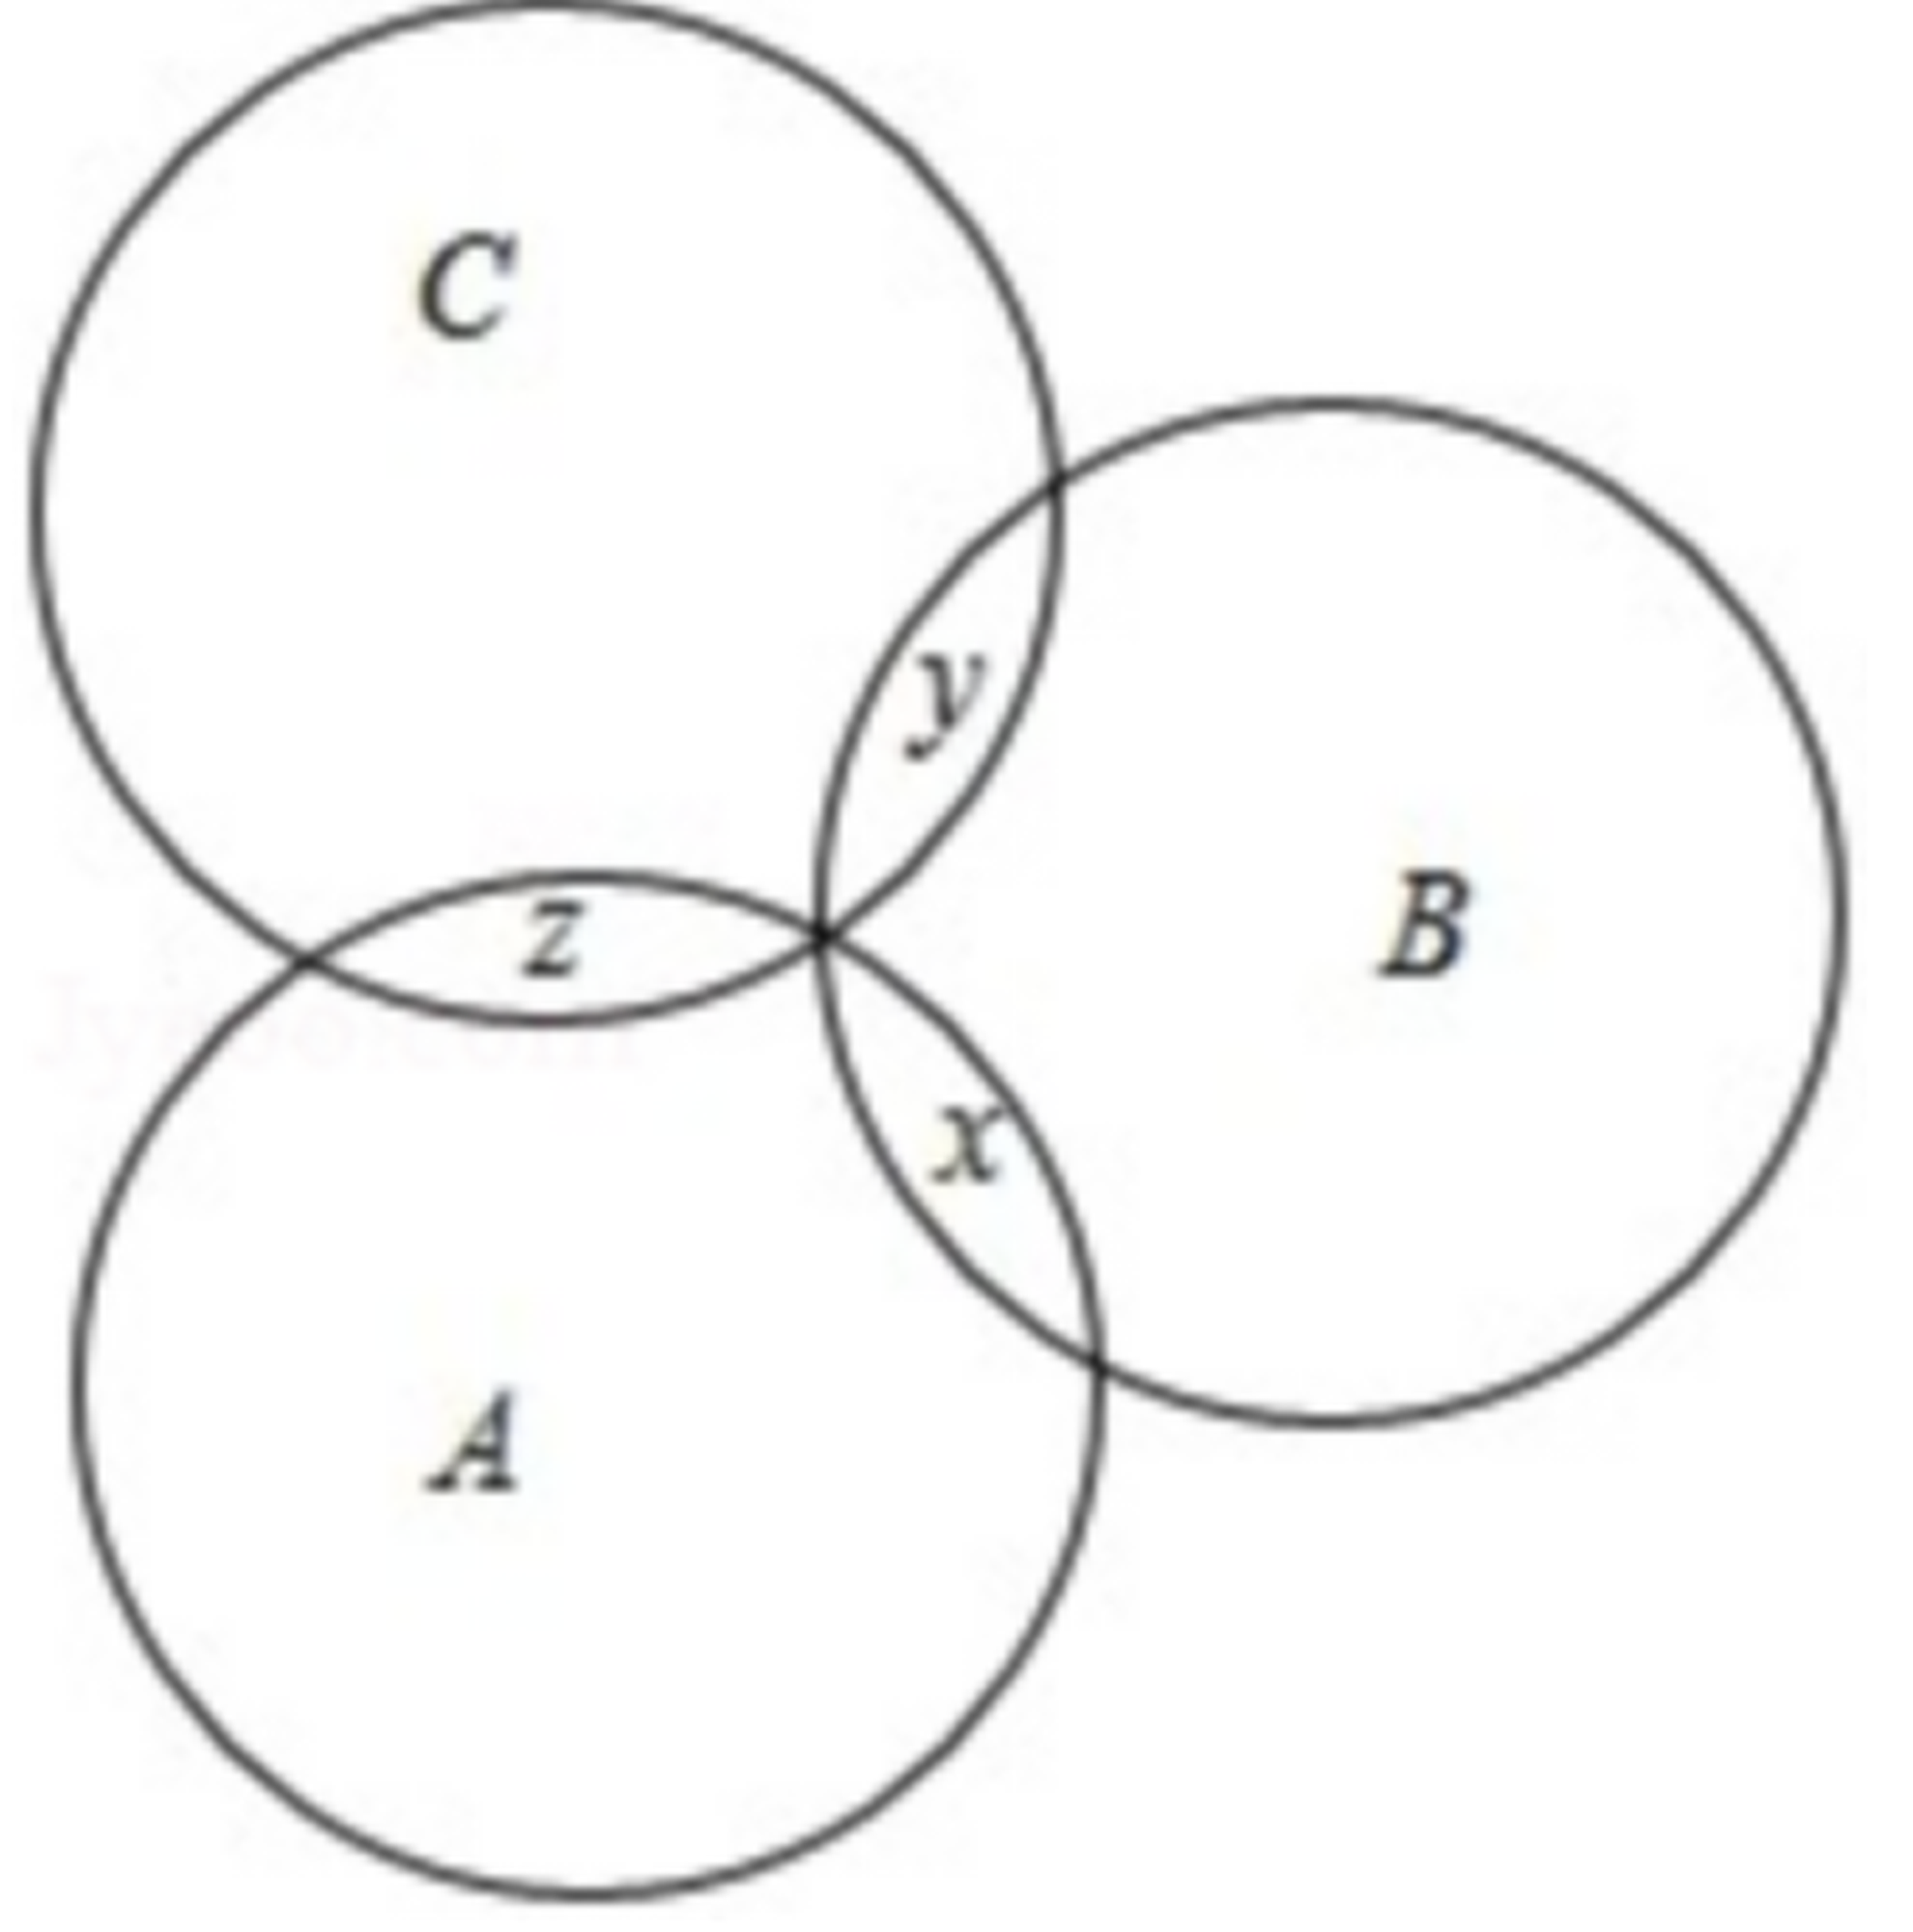
\includegraphics[width=0.30\textwidth]{figures/venn_ABC_x_y_z_h39.png}
\end{center}
\step{因为 $|A\cap B|=|B\cap C|=|C\cap A|=1$，且 $x$、$y$、$z\in\{1,2,3\}$，}
\step{所以集合 $A=\{x,z\}$，$B=\{x,y\}$，$C=\{z,y\}$，}
\step{若 $x=1$，$y=2$，$z=3$，则 $A=\{1,3\}$，$B=\{1,3\}$，$C=\{2,3\}$，}
\step{将 $1$，$2$，$3$ 进行全排列，有 $P_3^3=3\times2=6$ 个.}
\solend

\fi

\item 已知集合 $T=\{1,2,\cdots,2025\}$，对于 $T$ 的每一个非空子集的所有元素，计算它们乘积的倒数，
则所有这样倒数的和为 \blankline[4.4em].

\ans{$2025$}

\ifanswer
\solbegin
\step{集合 $T=\{1,2,\cdots,2025\}$ 的非空子集的个数为 $2^{2025}-1$，}
\step{这些子集中，每个元素的乘积分别为}
\step{$1,2,3,\cdots,2025,1\times2,1\times3,\cdots,1\times2025,\cdots,1\times2\times3\times\cdots\times2025$，}
\step{每项都可以看作是从 $1,2,3,\cdots,2025$ 中选择若干项的乘积，}
\step{$1+\dfrac12+\cdots+\dfrac{1}{2025}+\dfrac{1}{1\times2}+\dfrac{1}{1\times3}+\cdots+\dfrac{1}{2024\times2025}
+\cdots+\dfrac{1}{1\times2\times\cdots\times2025}$}
\step{$=(1+1)\left(1+\dfrac12\right)\cdots\left(1+\dfrac{1}{2025}\right)-1
=2\times\dfrac32\times\dfrac43\times\cdots\times\dfrac{2026}{2025}-1=2025$.}
\solend

\fi

% 第 24 题是压轴题，题干较长；试卷版在它之前量一次页高，尽量不与前文分家（照全稿成例）。
\ansneed{5cm}
% 注：原卷【解析】①③ 两步把 $f(x)$ 印作 $f[x[x]]$，显系笔误，照录未改，见文件头「笔误/存疑」⑦。
\item 若 $X$ 是一个集合，$T$ 是一个以 $X$ 的某些子集为元素的集合，且满足：①$X$ 属于 $T$，
$\varnothing$ 属于 $T$；②$T$ 中任意多个元素的并集属于 $T$；③$T$ 中任意多个元素的交集属于 $T$.
则称 $T$ 是集合 $X$ 上的一个拓扑. 已知函数 $f(x)=[x[x]]$，其中 $[x]$ 表示不大于 $x$ 的最大整数，
当 $x\in(0,n]$，$n\in\N^*$ 时，函数 $f(x)$ 值域为集合 $A_n$，则集合 $A_2$ 上的含有 $4$ 个元素的
拓扑 $T$ 的个数为 \blankline[4.4em].

\ans{$9$}

\ifanswer
\solbegin
\step{由题意，$n=2$，故 $0<x\leqslant2$，}
\step{①当 $0<x<1$ 时，则 $[x]=0$，所以 $f[x[x]]=0$，}
\step{②当 $x=1$ 时，$[x]=1$ 显然 $f(1)=1$，}
\step{③当 $1<x<2$ 时，$[x]=1$，所以 $f[x[x]]=[x]=1$，}
\step{④当 $x=2$ 时，$f(2)=4$，}
\step{所以 $A_2=\{0,1,4\}$，}
\step{因为 $T$ 中含有 $4$ 个元素，其中两个元素 $\varnothing$ 和 $A_2$，}
\step{$A_2=\{0,1,4\}$. 其它两个元素为 $A$、$B$，则
$\begin{cases}A\neq\varnothing\\ A\neq A_2\\ B\neq\varnothing\\ B\neq A_2\\ A\neq B\end{cases}$，}
\step{由对称性，不妨设 $1\leqslant|A|\leqslant|B|\leqslant2$，其中 $|A|$、$|B|$ 表示集合 $A$ 中元素的个数，}
\step{因为 $\begin{cases}A\cap B\in T\\ A\cup B\in T\end{cases}$，又 $|A|\leqslant|B|$，所以 $A\cap B=\varnothing$ 或 $A$，}
\step{若 $A\cap B=\varnothing$，则 $A\cup B$ 只能等于 $A_2$，}
\step{（若 $A\cup B=B$，则 $A\sub B$，则 $A\cap B=A=\varnothing$，矛盾）}
\step{则必有 $\begin{cases}|A|=1\\ |B|=2\end{cases}$，所以 $(A,B)$ 的个数 $\Leftrightarrow$ $A$ 的个数 $=3$ 种，}
\step{即 $\begin{cases}A=\{0\}\\ B=\{1,4\}\end{cases}$ 或 $\begin{cases}A=\{1\}\\ B=\{0,4\}\end{cases}$
或 $\begin{cases}A=\{4\}\\ B=\{0,1\}\end{cases}$；}
\step{若 $A\cap B=A\Leftrightarrow A\sub B$ 此时满足 $A\cup B=B$，}
\step{因为 $A\neq B$ 且 $1\leqslant|A|$ 且 $|B|\leqslant2$，所以 $\begin{cases}|A|=1\\ |B|=2\end{cases}$，}
\step{所以 $B$ 的选择共有 $C_3^2=3$ 种，则 $A$ 的个数有 $C_2^1$ 种，}
\step{所以 $(A,B)$ 的个数 $=2\times3=6$ 种.}
% 这六组「$A$／$B$」按原卷排作两行（前五个一行、第六个另起一行）；因五组并排时
% amsmath 的 cases 会为每组的第二列各留一枚 \quad，本行改排 \left\{\begin{matrix}…\end{matrix}\right.
% 以省下这枚 \quad（照 README「说明」记的高一07 成例），字形与 cases 相同。
\step{（这 $6$ 种是 $\left\{\begin{matrix}A=\{0\}\\ B=\{0,1\}\end{matrix}\right.$、
$\left\{\begin{matrix}A=\{1\}\\ B=\{0,1\}\end{matrix}\right.$、
$\left\{\begin{matrix}A=\{0\}\\ B=\{0,4\}\end{matrix}\right.$、
$\left\{\begin{matrix}A=\{4\}\\ B=\{0,4\}\end{matrix}\right.$、
$\left\{\begin{matrix}A=\{1\}\\ B=\{1,4\}\end{matrix}\right.$、}
\step{$\left\{\begin{matrix}A=\{4\}\\ B=\{1,4\}\end{matrix}\right.$）.}
\step{综上，$T$ 的个数为 $9$ 个.}
\solend

\fi

\end{enumerate}

\end{document}
"
%
% 原始材料是微信公众号图文（公众号「魔都数学加油站」连载「27学年高一 39」，署名「破晓」，
% 2026-09-26 21:29 发布，原文标题「27学年高一39——2026-2027年上海市大同中学高一上周末作业4.1」，
% 原文链接 https://mp.weixin.qq.com/s/HR2hIayXUXNi4zTs3PioiQ ），正文为 11 张 PNG 页。**同一篇里各页分辨率不一致**（2560×3620 与 4762×6735 两档混排：第 1、3、8、10 页为
% 2560×3620，第 2、4、5、6、7、9、11 页为 4762×6735）。原文本身就是一份**讲评版**——除第 15 题
% 外各题题下直接印【解析】（无单独的【答案】行），第 15 题的答案「D」直接印在题干末尾的括号内。
% 试题文字、答案与解析均照原卷录入，未改内容。卷面的粉色斜水印「魔都数学加油站」属水印，未录入。
%
% 卷首标题：原卷页首印作「2026-2027 年大同中学高一上周末作业 4.1」（**卷面标题行即带校名**，
% 年份区间按全稿惯例排 en dash，前缀照原卷保留「年」）。
%
% 篇幅与题号：卷面自「一、填空题」的**第 3 题**起编，终于「附加题」的**第 24 题**，共 22 题
% （填空 3—12、选择 13—16、解答 17—20、附加题 21—24）。第 1、2 题未在该文中发布——这是该
% 公众号连载讲评版的通例（高一02—高一09 等均自第 3 题起编，README「说明」已记），**不是截断**，
% 故本稿题号亦自 3 起。它与 高一40（大同中学 周末作业4.2）同属「周末作业 4」系列但**各自独立起编**
% （4.2 自第 3 题起、终于第 19 题），不是同一份试卷的两半。
%
% 与原卷的排版差异（均已在 README「说明」中交代）：
%   ① 原文自**第 3 题**起（第 1、2 题未在该文中发布），故本稿题号亦自 3 起，填空题以
%      \setcounter{enumi}{2} 起编；选择、解答、附加题三节各按上一节末号另设 \setcounter
%      （选择题 \setcounter{enumi}{12}、解答题 \setcounter{enumi}{16}、附加题 \setcounter{enumi}{20}）；
%   ② 原卷本就印有「一、填空题」「二、选择题」「三、解答题」三节标题，末节印作「附加题」
%      （**不带「四、」**，且题号 21—24 续前编、不另起），本稿照原卷分节，只把标题改排成全稿
%      统一的「大节标题」样式；
%   ③ 原卷是「讲评版」：除第 15 题外，各题题下均印【解析】（**全卷无一条独立的【答案】行**）；
%      第 15 题无解析，答案「D」直接印在题干末尾的括号内。本稿统一改为试卷版隐去、答案版以
%      \ans{}／\ifanswer 块给出，两版彻底分离；原卷写在【解析】末句的结果，本稿照 高一38
%      （同校同系列、同为讲评版）的成例另提为 \ans{}；
%   ④ 数集记号原卷两套并用：实数集作斜体的 $R$（第 7、11、14、17、18、19 题），整数集作斜体
%      $Z$（第 10 题），自然数集作斜体 $N$ 及 $N^*$（第 16、20、21、24 题），本稿按全稿惯例
%      统一写作 $\R$、$\Z$、$\N$、$\N^*$；
%   ⑤ 补集符号原卷两套并用：第 7 题作前缀式的 $C_U$（且题干称全集为 $I$，见「笔误/存疑」①），
%      第 14、15、18 题作上横线（$\overline{H}$、$\overline{A}$、$\overline{B}$），本稿照录、不归一
%      （前缀式写作 $\complement_U$，与 高一c／高一10 的成例一致）；
%   ⑥ 包含符号原卷两套并用：第 3 题作**无下划线**的 $\subset$，第 15、18、20、24 题作**带下划线**
%      的 $\sub$，本稿照录、不归一；
%   ⑦ 原卷填空的横线约两个字宽，本稿按全稿惯例统一排 \blankline[4.4em]；
%   ⑧ 第 7、11、22 题各有插图，取原卷截图、4× LANCZOS 放大（figures/venn_N_cap_CI_M_h39.png、
%      figures/plane_grid_4squares_h39.png、figures/venn_ABC_x_y_z_h39.png）；第 7 题的 Venn 属
%      **题干**（试卷版、答案版都出），第 11、22 题的图在【解析】内（仅答案版出）。第 7 题图
%      左下、第 11 题图的上／左／右边缘带进极淡的原卷粉色水印残影——照全稿「插图直接取自
%      原卷截图、不用 TikZ 重绘、不修图」的体例保留（再裁会切到坐标轴与 $x$、$y$、$O$ 标注）；
%   ⑨ 原卷并列的字母、数字（「$x_1,x_2$」「$a,b$」「$1,2,3,\cdots,11$」）多作半角逗号或不加标点，
%      本稿按全稿惯例改排顿号（$x_1$、$x_2$）或把数列并入行内公式；半角括号、逗号一律排全角，
%      数学式内部的标点照原样；
%   ⑩ 原卷未印副标题，本稿按**本卷实际内容**补出副标题「集合与常用逻辑用语」（依据见下条）。
%
% 副标题（\examtitlest 第二个参数）：本卷卷面未印副标题，由本稿补出，取值按 2026-09-26 起的
%   新口径「只用本卷实际内容的模块名」定为「集合与常用逻辑用语」。依据：全卷 22 题（第 3—24 题）中，
%   第 3、5、7、8、10、11、14、15、16、17、18、19、20、21、22、23、24 题共 17 题是集合的运算与
%   关系、子集／真子集、补集、集合新定义（「全食／偏食」、最小相交、拓扑、特征数）与集合计数，
%   以及命题与常用逻辑用语（第 3 题充要条件、第 5 题存在量词命题、第 17 题命题真假）；其余两题
%   第 4、6 考一元二次方程的根（韦达定理）与方程恒等，第 9、12、13 题是不等式（一元二次不等式组
%   的整数解、一元二次不等式解集、不等式的性质）——不等式合计 3/22，**不足全卷三分之一**，
%   故不并标「不等式」。
%
% 原卷笔误/存疑（均照抄原卷、未改，见源码中该处上方注释）：
%   ① 第 7 题题干称「全集 $I=R$」，而【解析】两处把补集写作 $C_U M$（下标作 $U$），前后记号不一；
%      本稿照录，未改；
%   ② 第 4 题【解析】两处把判别式印作 $\triangle=[2(m-1)^2-16m^2]$（方括号内首项漏了平方，
%      正确应作 $[2(m-1)]^2-16m^2$）；按其所判「$m=\frac12$ 时 $<0$、$m=-\frac12$ 时 $>0$」反推，
%      $[2(m-1)]^2-16m^2$ 在 $m=\frac12$ 时为 $-3<0$、在 $m=-\frac12$ 时为 $5>0$，与结论一致；
%      本稿照录；
%   ③ 第 9 题【解析】把方程组第二式印作 $1-2<-k\leqslant3$，按其结论 $-3\leqslant k<2$ 反推，
%      疑当作 $-2<-k\leqslant3$（原卷多一个「$1$」）；本稿照录；
%   ④ 第 17 题【解析】首句「由数 $y=-x^2+ax-1=-x+3$」中的「由数」显系「由」或「由函数」之误；
%      且末段「若 $p$ 真 $q$ 假…得 $a\in R$」「若 $p$ 假 $q$ 真…此时 $a$ 无解」与结论「$a$ 的取值范围
%      是 $R$」自相矛盾（按 $p:a\leqslant-5$、$q:a>-6$，$p$ 真 $q$ 假应为 $a\leqslant-6$，$p$ 假 $q$ 真
%      应为 $a>-5$，合起来是 $a\leqslant-6$ 或 $a>-5$，并非 $R$）；本稿一律照录，未按正确解法改写；
%   ⑤ 第 18 题【解析】(2) 把 $B=\{x\mid x^2+a\leqslant0\}$（$a<0$）印作右端开的
%      $\{x\mid-\sqrt{-a}\leqslant x<\sqrt{-a}\}$（应为闭的「$\leqslant$」）；按其所判
%      $\sqrt{-a}<\frac12$ 反推，不影响结论；本稿照录；
%   ⑥ 第 22 题【解析】在 $x=1$、$y=2$、$z=3$ 时把 $B=\{x,y\}$ 印作 $\{1,3\}$（应为 $\{1,2\}$），
%      与本行前面「$B=\{x,y\}$」不合；本稿照录；
%   ⑦ 第 24 题【解析】①③ 两步把 $f(x)$ 印作 $f[x[x]]$，显系笔误；本稿照录。
%   ⑧ 第 8 题【解析】「即方程 $x^2+ax+b=x$，$x^2+(a-1)x+b=0$ **由**两个相等的实数根为 $4$」——
%      「由」当为「有」（「设…是…有」的杂糅）；本稿照录；
%   ⑨ 第 10 题：题设 $a\oplus b=b(a^2+b^2+1)$，而集合定义里含 $\dfrac{a\oplus b}{2b}$；$-2<a<b<2$、
%      $a$、$b\in\Z$ 时 $(a,b)=(-1,0)$ 也合条件、却使分母 $2b=0$，原卷解析仍代入该组并约去
%      $b$ 得 $x=1$（答案集恰好不变）；本稿照录；
%   ⑩ 第 15 题选项列里 ② 与 ③ 之间**漏排分隔号**（原卷作「② $\overline{A}\cap B=\varnothing$③
%      $\overline{A}\sub\overline{B}$；」——①、③ 后都有「；」，② 后没有）；本稿照录；
%   ⑪ 第 20(2) 把 $\{1,2,\cdots,20\}$ 分成的 11 个集合里，$\{8,11\}$ 与 $\{9,12\}$ 之间误用
%      **句号**「.」（同行其余处皆逗号）；本稿照录；
%   ⑫ 第 20(3)① 推理不严：原卷写「选 5 则不选 1、9；选 6 则不选 2、10；选 7 则不选 3、11；
%      则只剩 4、8」——但 4 与 8 相差 $4$、不能同选，该情形实际最多只能取 $4$ 个；末句结论
%      「不超过 $5$ 个」仍成立；本稿照录；
%   ⑬ 第 16 题【解析】两种下标并存：「所以在 $A_i$ 的特征数构成中」原卷作斜体 $A_i$，而
%      「要使 $X_1+X_2+X_3$ 最大（小），则（应）在集合 $A_1$ 中首先放置…」两处原卷作
%      **数字 $1$**（与同句 $X_1$ 的角标同形）；本稿照录、未归一。
%
% 图取原卷截图（依次见各处的 \includegraphics 前的注释），4× LANCZOS 放大。
\documentclass[a4paper,11pt]{article}
\usepackage{common}

\begin{document}

\examtitlest[3]{2026--2027 年大同中学高一上周末作业 4.1}{集合与常用逻辑用语}

\bigsec{一、填空题}

\begin{enumerate}
\setcounter{enumi}{2}

\item “$x\geqslant a$”是“$0<x<2$”的必要非充分条件，则实数 $a$ 的取值范围是 \blankline[4.4em].

\ans{$(-\infty,0]$}

\ifanswer
\solbegin
\step{因为 $x\geqslant a$ 是 $0<x<2$ 的必要非充分条件，所以 $(0,2)\subset[a,+\infty)$，所以 $a\leqslant0$，}
\step{则实数 $a$ 的取值范围是 $(-\infty,0]$.}
\solend

\fi

% 注：原卷$[2(m-1)^2-16m^2]$ 首项漏了平方（应为 $[2(m-1)]^2-16m^2$），照录未改，见文件头「笔误/存疑」②。
\item 若关于 $x$ 的方程 $x^2+2(m-1)x+4m^2=0$ 有两个实数根，且这两根互为倒数，则 $m=$ \blankline[4.4em].

\ans{$-\dfrac12$}

\ifanswer
\solbegin
\step{设 $x_1$、$x_2$ 是方程 $x^2+2(m-1)x+4m^2=0$ 有两个实数根，}
\step{则 $x_1x_2=4m^2=1$，解得 $m=\dfrac12$ 或 $m=-\dfrac12$，}
\step{又当 $m=\dfrac12$ 时，$\triangle=[2(m-1)^2-16m^2]<0$，舍去，}
\step{当 $m=-\dfrac12$ 时，$\triangle=[2(m-1)^2-16m^2]>0$，故 $m=-\dfrac12$.}
\solend

\fi

\item 已知命题：“存在 $x\in[1,2]$，使 $x^2+2x+a\geqslant0$”为真命题，则 $a$ 的取值范围是 \blankline[4.4em].

\ans{$a\geqslant-8$}

\ifanswer
\solbegin
\step{若存在 $x\in[1,2]$，使 $x^2+2x+a\geqslant0$，}
\step{则等价为存在 $x\in[1,2]$，使 $x^2+2x\geqslant-a$，}
\step{当存在 $x\in[1,2]$ 时，设 $y=x^2+2x=(x+1)^2-1$，则 $3\leqslant y\leqslant8$，}
\step{所以要使 $x^2+2x\geqslant-a$，则 $8\geqslant-a$，即 $a\geqslant-8$.}
\solend

\fi

\item 已知方程 $a(3x+2)+b(2x-3)=8x+3$ 有无穷多个解，则 $a:b=$ \blankline[4.4em].

\ans{$30:7$}

\ifanswer
\solbegin
\step{$a(3x+2)+b(2x-3)=(3a+2b)x+2a-3b=8x+3$ 有无穷多个解，}
\step{所以 $\begin{cases}3a+2b=8\\ 2a-3b=3\end{cases}$，解得 $a=\dfrac{30}{13}$，$b=\dfrac{7}{13}$，所以 $a:b=30:7$.}
\solend

\fi

% 注：原卷题干称「全集 $I=R$」，而【解析】两处把补集写作 $C_U M$（下标作 $U$），前后记号不一；
%     照录未改，见文件头「笔误/存疑」①。
\item 已知集合 $M=\{x\mid y=\sqrt{3-x^2}\}$，$N=\{x\mid-3\leqslant x\leqslant1\}$，全集 $I=\R$，
则图中阴影部分表示的集合为 \blankline[4.4em].

% 图取原卷截图（01.png，2560×3620）右栏，4× LANCZOS 放大。
\begin{center}
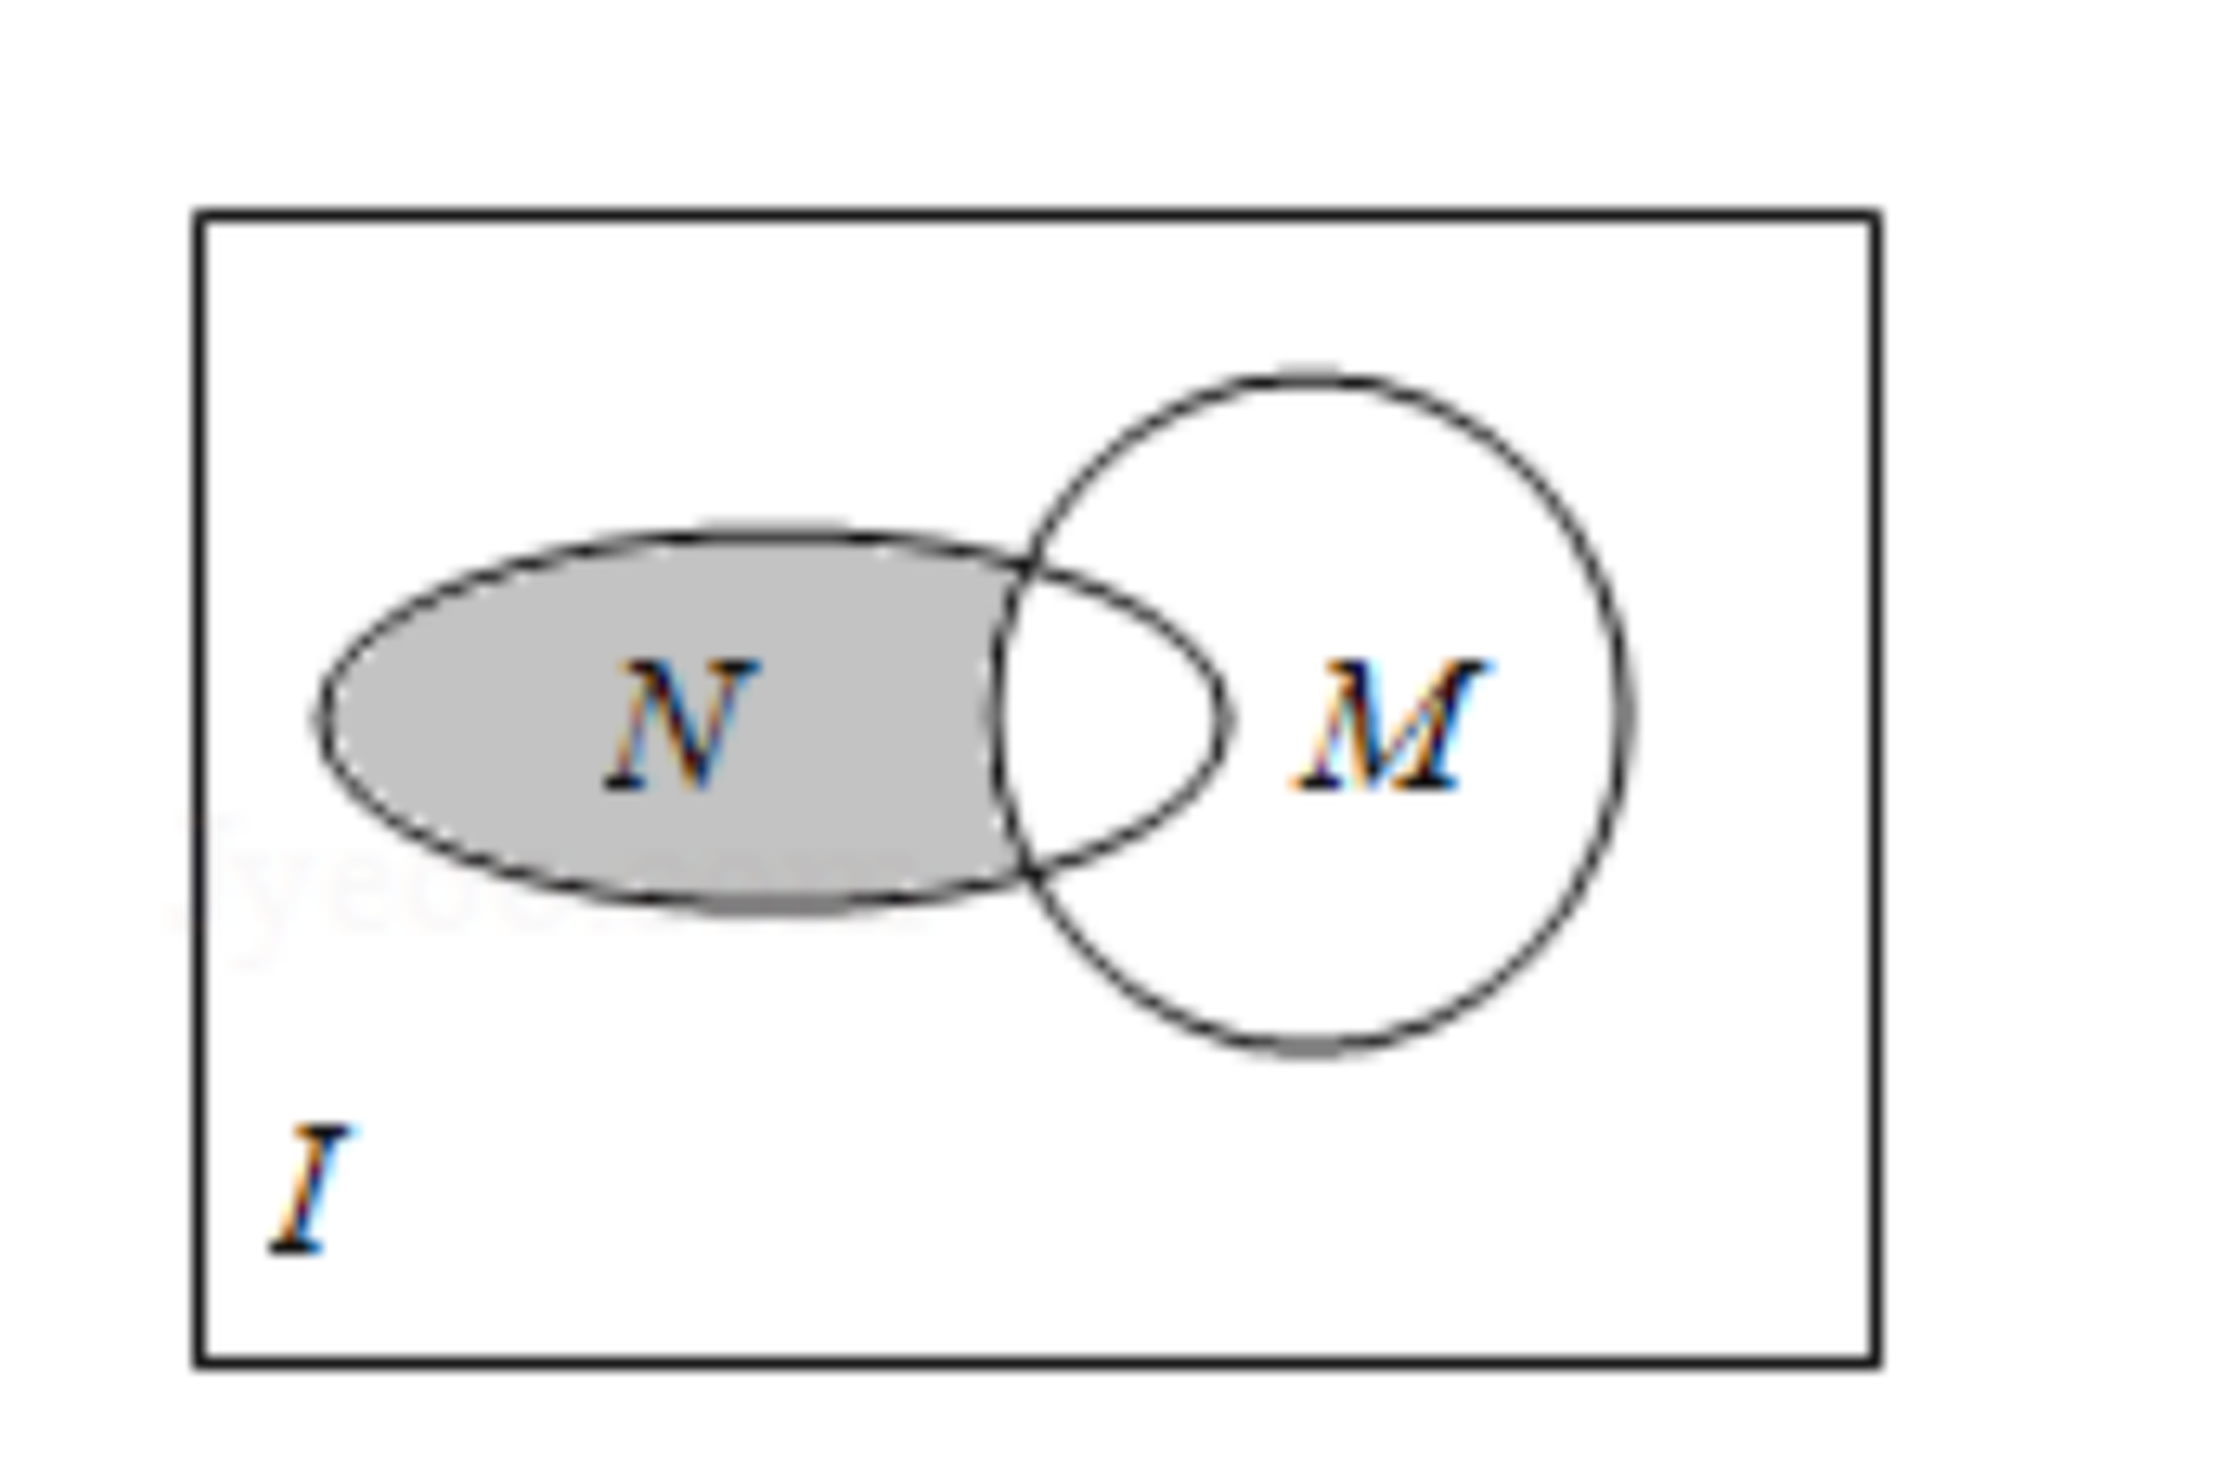
\includegraphics[width=0.30\textwidth]{figures/venn_N_cap_CI_M_h39.png}
\end{center}

\ans{$[-3,-\sqrt3)$}

\ifanswer
\solbegin
\step{阴影部分用集合表示为 $N\cap(\complement_UM)$.}
\step{则 $M=\{x\mid y=\sqrt{3-x^2}\}=\{x\mid3-x^2\geqslant0\}=\{x\mid-\sqrt3\leqslant x\leqslant\sqrt3\}$，}
\step{则 $\complement_UM=\{x\mid x>\sqrt3\text{ 或 }x<-\sqrt3\}$，$N=\{x\mid|x+1|\leqslant2\}=\{x\mid-3\leqslant x\leqslant1\}$，}
\step{则 $N\cap(\complement_UM)=\{x\mid-3\leqslant x<-\sqrt3\}$.}
\solend

\fi

\item 已知 $f(x)=x^2+ax+b$，集合 $\{x\mid f(x)=x\}=\{4\}$，将集合 $M=\{x\mid f(x)=4\}$ 用列举法表示 \blankline[4.4em].

\ans{$\{3,4\}$}

\ifanswer
\solbegin
\step{已知 $f(x)=x^2+ax+b$，集合 $\{x\mid f(x)=x\}=\{4\}$，}
% 注：原卷本行作「…$x^2+(a-1)x+b=0$ **由**两个相等的实数根为 $4$」——「由」当为「有」
%     （「设…是…有」的杂糅）；本稿照录未改，见文件头「原卷笔误/存疑」⑧。
\step{即方程 $x^2+ax+b=x$，$x^2+(a-1)x+b=0$ 由两个相等的实数根为 $4$，}
\step{所以 $\triangle=(a-1)^2-4b=0$，即 $x^2+(a-1)x+b=(x-4)^2$，所以 $b=16$，$a=-7$，}
\step{所以 $f(x)=x^2+ax+b=x^2-7x+16$，所以集合 $M=\{x\mid f(x)=4\}$，}
\step{即 $x^2-7x+16=4$，$x^2-7x+12=0$，故 $M=\{x\mid f(x)=4\}=\{3,4\}$.}
\solend

\fi

% 注：原卷方程组第二式印作 $1-2<-k\leqslant3$，按其结论 $-3\leqslant k<2$ 反推疑当作 $-2<-k\leqslant3$，
%     照录未改，见文件头「笔误/存疑」③。
\item 关于 $x$ 的不等式组 $\begin{cases}x^2-x-2>0\\ 2x^2+(2k+5)x+5k<0\end{cases}$ 的整数解的集合为 $\{-2\}$，
则实数 $k$ 的取值范围 \blankline[4.4em].

\ans{$-3\leqslant k<2$}

\ifanswer
\solbegin
\step{原不等式组即 $\begin{cases}(x-2)(x+1)>0\\ (x+k)(2x+5)<0\end{cases}$，整数解的集合为 $A$，若 $A=\{-2\}$，}
\step{则 $(-2+k)(2\times(-2)+5)<0$，所以 $k<2$，且有 $\begin{cases}-k>-\dfrac52\\ 1-2<-k\leqslant3\end{cases}$，}
\step{解得 $-3\leqslant k<2$.}
\solend

\fi

\item 规定 $\oplus$ 与 $\otimes$ 是两个运算符号，其运算法则如下，对任意实数 $a$、$b$ 有：$a\otimes b=ab$，
$a\oplus b=b(a^2+b^2+1)$. 若 $-2<a<b<2$ 且 $a$、$b\in\Z$，
$A=\left\{x\mid x=2(a\otimes b)+\dfrac{a\oplus b}{2b}\right\}$，则用列举法表示集合 $A=$ \blankline[4.4em].

\ans{$\left\{1,-\dfrac12\right\}$}

\ifanswer
\solbegin
\step{$A=\left\{x\mid x=2(a\otimes b)+\dfrac{a\oplus b}{2b}\right\}
=\left\{x\mid x=2ab+\dfrac{b(a^2+b^2+1)}{2b}\right\}$}
\step{$=\left\{x\mid x=2ab+\dfrac12a^2+\dfrac12b^2+\dfrac12\right\}
=\left\{x\mid x=\dfrac12(a+b)^2+ab+\dfrac12\right\}$，}
% 注：题设含 $\dfrac{a\oplus b}{2b}$，而 $-2<a<b<2$、$a$、$b\in\Z$ 时 $(a,b)=(-1,0)$ 也合条件、
%     却使分母 $2b=0$；原卷解析仍代入该组并约去 $b$ 得 $x=1$（答案集恰好不变）。本稿照录，
%     见文件头「原卷笔误/存疑」⑨。
\step{当 $a=-1$，$b=0$ 时，$x=1$；当 $a=-1$，$b=1$ 时，$x=-\dfrac12$；}
\step{当 $a=0$，$b=1$ 时，$x=1$；所以 $A=\left\{1,-\dfrac12\right\}$.}
\solend

\fi

\item 高斯是德国著名的数学家，近代数学奠基者之一，享有“数学王子”的称号，为了纪念数学家高斯，
我们把取整函数 $y=[x]$，$x\in\R$ 称为高斯函数，其中 $[x]$ 表示不超过 $x$ 的最大整数，
如 $[1.1]=1$，$[-1.1]=-2$. 则点集 $P=\{(x,y)\mid[x]^2+[y]^2=1\}$
所表示的平面区域的面积是 \blankline[4.4em].

\ans{$4$}

\ifanswer
\solbegin
\step{$[x]^2+[y]^2=1$ 由 $\begin{cases}[x]=0\\ [y]=-1\end{cases}$ 或 $\begin{cases}[x]=0\\ [y]=1\end{cases}$
或 $\begin{cases}[x]=-1\\ [y]=0\end{cases}$ 或 $\begin{cases}[x]=1\\ [y]=0\end{cases}$ 四个平面区域组成，}
\step{即 $\begin{cases}0\leqslant x<1\\ -1\leqslant y<0\end{cases}$ 或 $\begin{cases}0\leqslant x<1\\ 1\leqslant y<2\end{cases}$
或 $\begin{cases}-1\leqslant x<0\\ 0\leqslant y<1\end{cases}$ 或 $\begin{cases}1\leqslant x<2\\ 0\leqslant y<1\end{cases}$，}
\step{作出平面区域如图所示，平面区域由四个边长为 $1$ 的正方形组成，}
% 图在【解析】内（仅答案版出），取原卷截图（03.png，2560×3620）中部，4× LANCZOS 放大。
\begin{center}
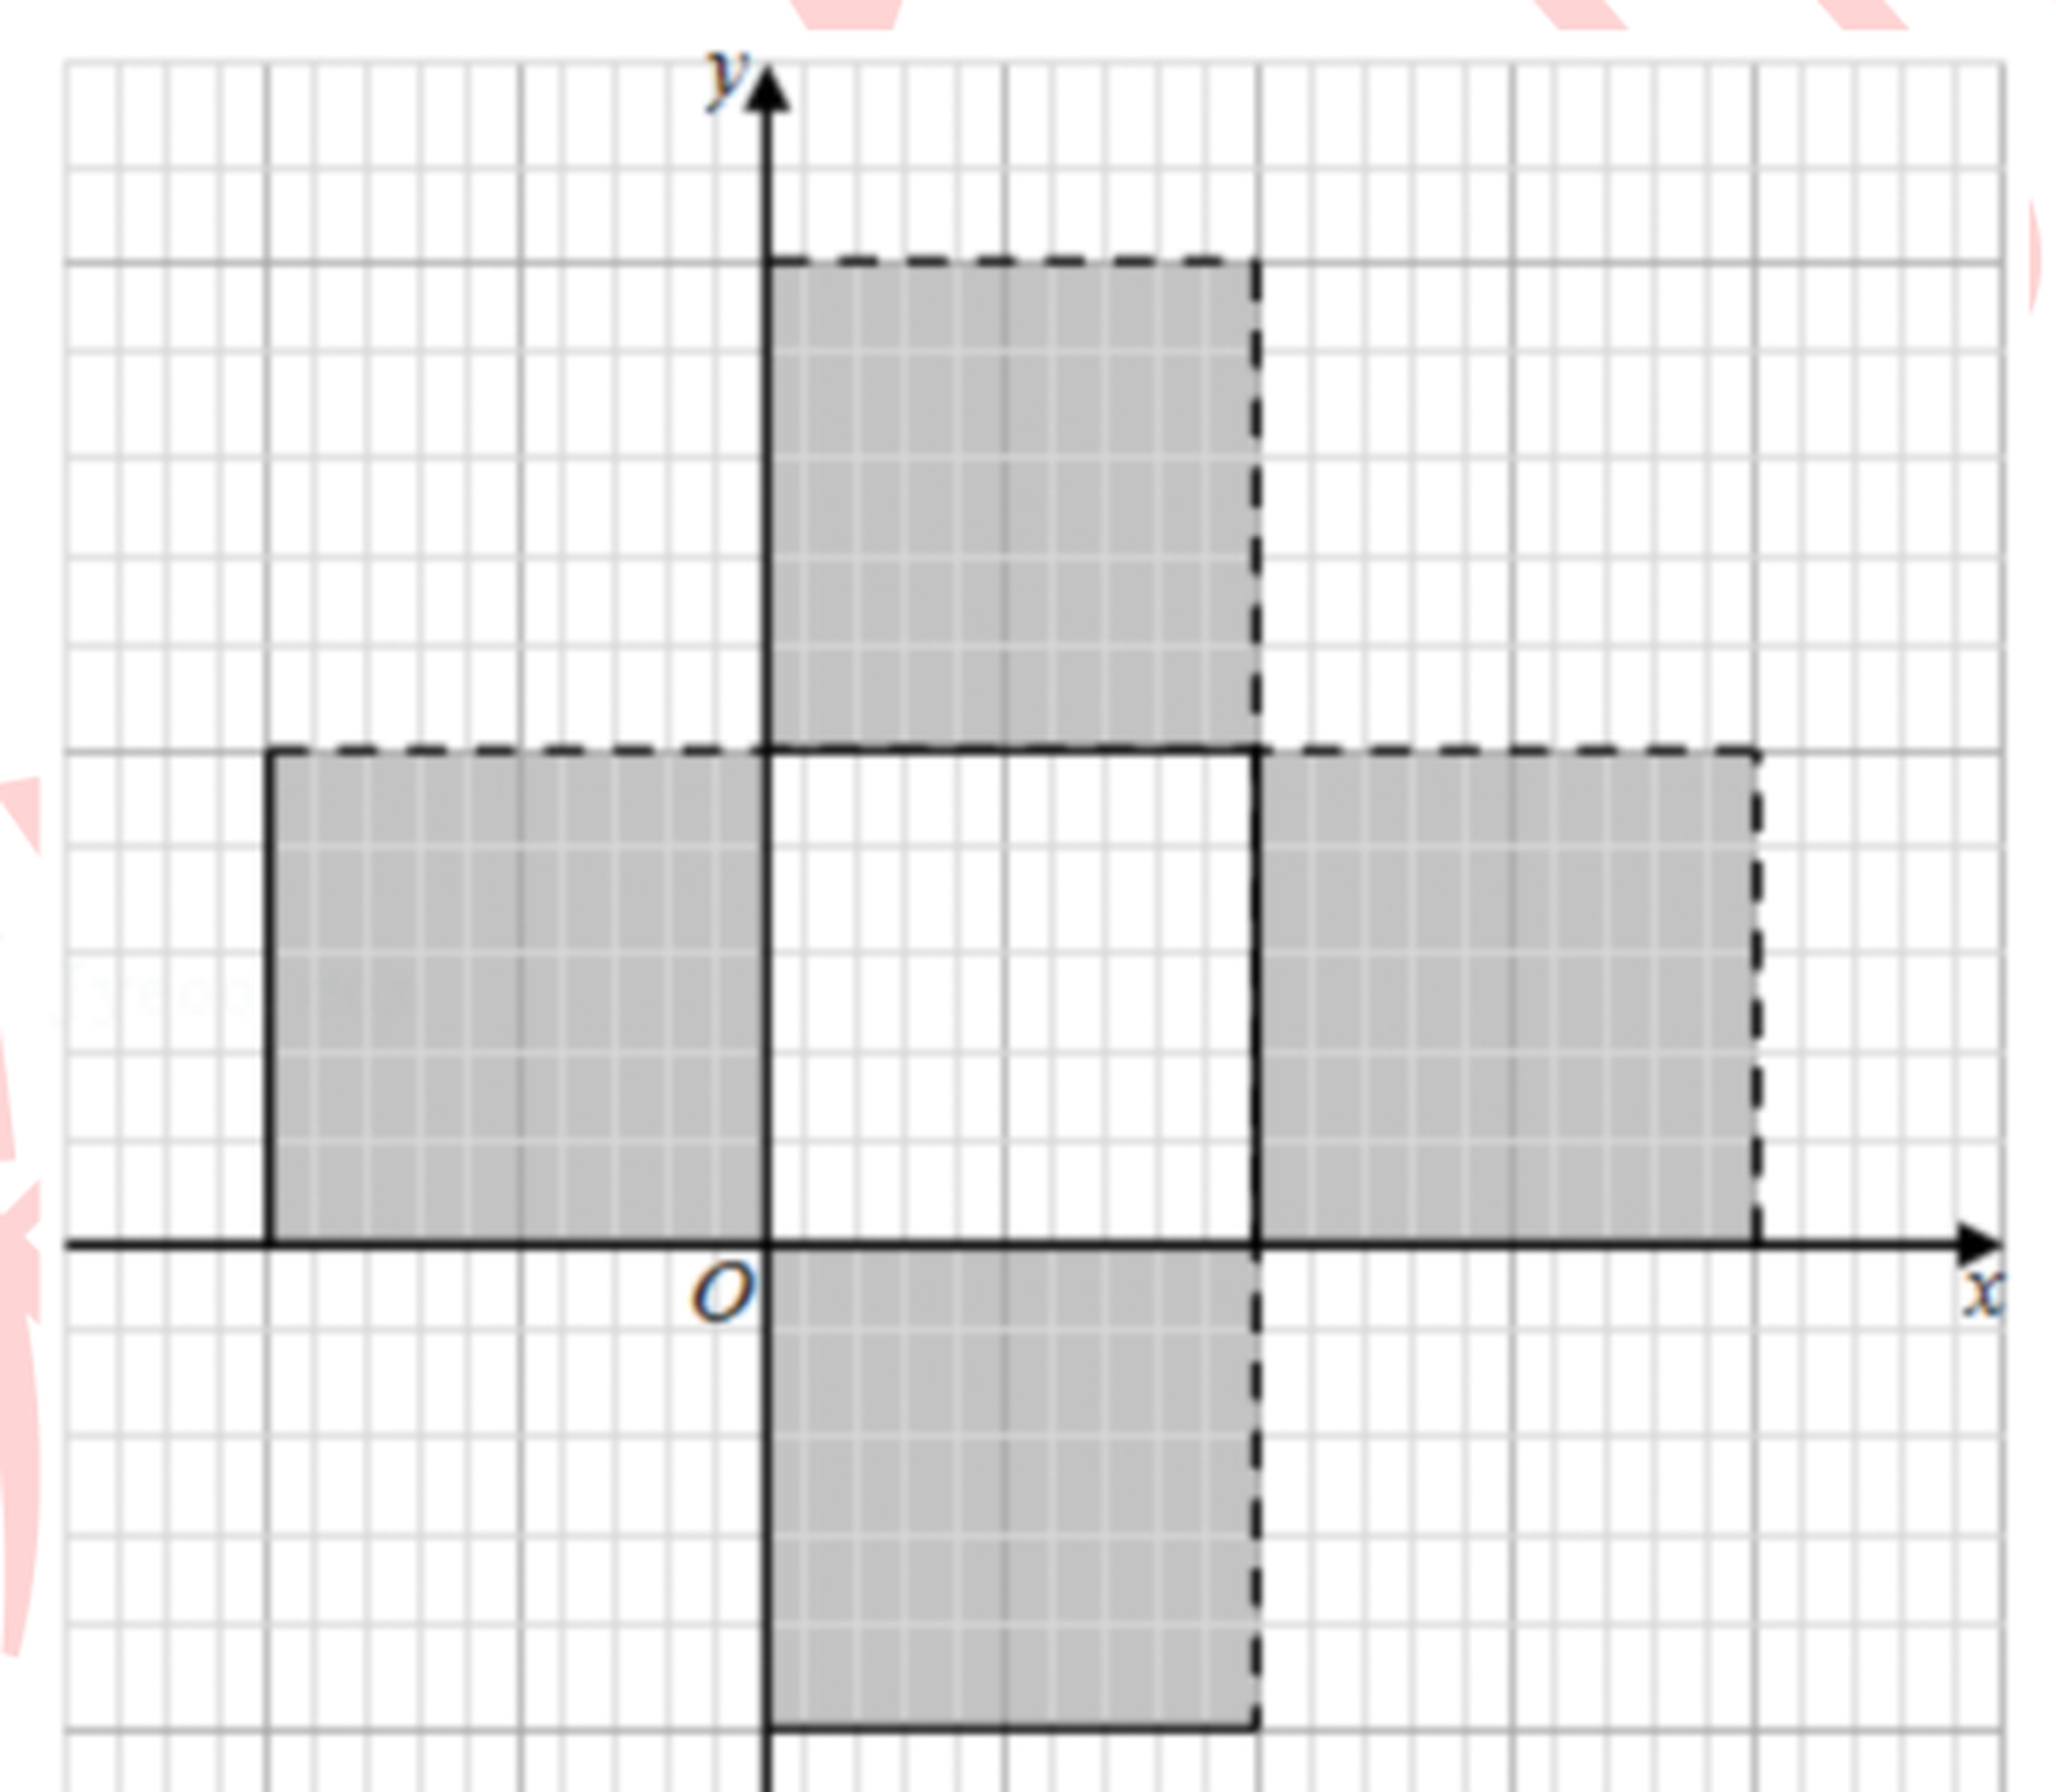
\includegraphics[width=0.38\textwidth]{figures/plane_grid_4squares_h39.png}
\end{center}
\step{总面积为 $1\times4=4$.}
\solend

\fi

\item 关于 $x$ 的不等式 $ax^2+bx+c>0$ 的解集为 $\{x\mid x<\beta\text{ 或 }x>\gamma\}(0<\beta<\gamma)$，
则不等式 $a(x^2+1)+b(x-1)+c>2ax$ 的解集为 \blankline[4.4em].

\ans{$(-\infty,\beta+1)\cup(\gamma+1,+\infty)$}

\ifanswer
\solbegin
\step{由题意得 $\beta$、$\gamma$ 为方程 $ax^2+bx+c=0$ 的两根且 $a>0$，}
\step{则 $\beta+\gamma=-\dfrac ba$，$\beta\gamma=\dfrac ca$，故 $b=-a(\beta+\gamma)$，$c=\beta\gamma a$，}
\step{则不等式可化为 $a(x^2+1)-a(\beta+\gamma)(x-1)+\beta\gamma a>2ax$，}
\step{因为 $a>0$，所以 $x^2+1-(\beta+\gamma)(x-1)+\beta\gamma>2x$，}
\step{即 $x^2-(\beta+\gamma+2)x+(\beta+\gamma+\beta\gamma+1)>0$，所以 $(x-\beta-1)(x-\gamma-1)>0$，}
\step{解得 $x<\beta+1$ 或 $x>\gamma+1$，所以不等式解集为 $(-\infty,\beta+1)\cup(\gamma+1,+\infty)$.}
\solend

\fi

\end{enumerate}

\bigsec{二、选择题}

\begin{enumerate}
\setcounter{enumi}{12}

\item 设 $a<b<0$，则下列不等式中不成立的是\mbox{（\quad）}

\keepwithprev
A. $\dfrac1a>\dfrac1b$\qquad B. $\dfrac{1}{a-b}>\dfrac1a$\qquad C. $|a|>-b$\qquad D. $\sqrt{-a}>\sqrt{-b}$

\ans{$B$}

\ifanswer
\solbegin
\step{令 $a=-2$，$b=-1$，}
\step{A、$-\dfrac12>-1$，正确；B、$-1<-\dfrac12$，故 B 错误；C、$2>1$，正确；}
\step{D、$\sqrt2>1$，正确；故选 B.}
\solend

\fi

\item 设实数集 $\R$ 为全集，集合 $P=\{x\mid f(x)=0\}$，$Q=\{x\mid g(x)=0\}$，$H=\{x\mid h(x)=0\}$，
则方程 $\dfrac{f^2(x)+g^2(x)}{h(x)}=0$ 的解集是\mbox{（\quad）}

\keepwithprev
A. $P\cap Q\cap\overline{H}$\qquad B. $P\cap Q$\qquad C. $P\cap Q\cap H$\qquad D. $P\cap Q\cup H$

\ans{$A$}

\ifanswer
\solbegin
\step{方程 $\dfrac{f^2(x)+g^2(x)}{h(x)}=0$ 等价于 $\begin{cases}f(x)=0\\ g(x)=0\\ h(x)\neq0\end{cases}$，}
\step{又因为 $P=\{x\mid f(x)=0\}$，$Q=\{x\mid g(x)=0\}$，$H=\{x\mid h(x)=0\}$，}
\step{所以方程 $\dfrac{f^2(x)+g^2(x)}{h(x)}=0$ 的解集是 $P\cap Q\cap\overline{H}$，故选 A.}
\solend

\fi

\item 设全集 $U$，在下列条件中，是 $B\sub A$ 的充要条件的有\mbox{（\quad）}

\keepwithprev
% 注：原卷此行 ② 与 ③ 之间**漏排分隔号**（①、③ 后都有「；」，② 后没有）；
%     本稿照录未补，见文件头「原卷笔误/存疑」⑩。
①$A\cup B=A$；\qquad ②$\overline{A}\cap B=\varnothing$\qquad ③$\overline{A}\sub\overline{B}$；\qquad ④$A\cup\overline{B}=U$

\keepwithprev
A. $1$ 个\qquad B. $2$ 个\qquad C. $3$ 个\qquad D. $4$ 个

\ans{$D$}

\item 已知集合 $M=\{x\mid x\in\N,0<x\leqslant15\}$，$A_1$、$A_2$、$A_3$ 满足：①$A_1\cup A_2\cup A_3=M$；
②每个集合都恰有 $5$ 个元素. 集合 $A_i(i=1,2,3)$ 中最大元素与最小元素之和称为 $A_i$ 的特征数，
记为 $X_i(i=1,2,3)$，则 $X_1+X_2+X_3$ 的值不可能为\mbox{（\quad）}

\keepwithprev
A. $37$\qquad B. $39$\qquad C. $48$\qquad D. $57$

\ans{$A$}

\ifanswer
\solbegin
\step{因为集合 $M=\{x\mid x\in\N,0<x\leqslant15\}=\{1,2,3,\cdots,15\}$，}
\step{又因为集合 $A_1$、$A_2$、$A_3$ 中，每个集合恰有 $5$ 个元素，}
\step{且 $A_1\cup A_2\cup A_3=M$ 有 $15$ 个元素，所以集合 $A_1$、$A_2$、$A_3$ 中没有重复元素，}
\step{因为 $1$ 是集合 $M$ 中数值最小的元素，$15$ 是集合 $M$ 中数值最大的元素，}
\step{所以在 $A_i$ 的特征数构成中，必有 $1$ 和 $15$，不妨设 $1\in A_1$，$15\in A_1$，}
% 注：原卷本行（与下面「最小」那句）在「集合」后的角标是**数字 $1$**（同句 $X_1$ 的角标同形），
%     而非上一行「$A_i$ 的特征数构成」里的斜体 $A_i$——原卷两种下标并存，本稿照录、不归一，
%     见文件头「原卷笔误/存疑」⑬。
\step{要使 $X_1+X_2+X_3$ 最大，则应该在集合 $A_1$ 中首先放置数值较小的元素，}
\step{即 $A_1=\{1,2,3,4,15\}$，所以 $5$ 与 $14$ 是剩下元素中数值最小或最大的元素，}
\step{同理，不妨设 $5\in A_2$，$14\in A_2$，接着在 $A_2$ 中再次放置数值较小的元素，}
\step{即 $A_2=\{5,6,7,8,14\}$，则 $A_3=\{9,10,11,12,13\}$，}
\step{此时 $X_1+X_2+X_3$ 有最大值为 $1+15+5+14+9+13=57$，}
\step{即 $X_1+X_2+X_3\leqslant57$；}
% 注：同上一处——原卷此行角标是**数字 $1$**（$A_1$），本稿照录，未与「$A_i$」归一。
\step{要使 $X_1+X_2+X_3$ 最小，则在集合 $A_1$ 中首先放置数值较大的元素，}
\step{即 $A_1=\{1,12,13,14,15\}$，所以 $2$ 与 $11$ 是剩下元素中数值最小或最大的元素，}
\step{同理，不妨设 $2\in A_2$，$11\in A_2$，接着在 $A_2$ 中再次放置数值较大的元素，}
\step{即 $A_2=\{2,8,9,10,11\}$，则 $A_3=\{3,4,5,6,7\}$，}
\step{此时 $X_1+X_2+X_3$ 有最小值为 $1+15+2+11+3+7=39$，}
\step{即 $X_1+X_2+X_3\geqslant39$，}
\step{综上，$39\leqslant X_1+X_2+X_3\leqslant57$，故选 A.}
\solend

\fi

\end{enumerate}

\bigsec{三、解答题}

\begin{enumerate}
\setcounter{enumi}{16}

% 注：原卷首句「由数 $y=-x^2+ax-1=-x+3$」中的「由数」显系「由」或「由函数」之误；末段
%     的两处分类讨论与结论自相矛盾（详见文件头「笔误/存疑」④）。本稿一律照录，未改。
\item 命题 $p$：函数 $y=-x^2+ax-1$ 与 $y=-x+3$ 图象交点的横坐标均为负值，
命题 $q$：关于 $x$ 的方程 $2(1-x)a+(x^2-10x-3)=0$ 的两个根，一个大于 $3$，另一个小于 $3$；
若命题 $p$ 和命题 $q$ 中有且仅有一个是真命题，求 $a$ 的取值范围.

\ans{$\R$}

\ifanswer
\solbegin
\step{由数 $y=-x^2+ax-1=-x+3$ 得 $x^2-(a+1)x+4=0$，}
\step{若横坐标均为负值，则满足 $\begin{cases}\Delta=(a+1)^2-16\geqslant0\\ x_1x_2=4>0\\ x_1+x_2=a+1<0\end{cases}$
得 $\begin{cases}a\geqslant3\text{ 或 }a\leqslant-5\\ a<-1\end{cases}$，得 $a\leqslant-5$，}
\step{即 $p:a\leqslant-5$，}
\step{若方程 $2(1-x)a+(x^2-10x-3)=0$ 的两个根，一个大于 $3$，另一个小于 $3$；}
\step{设 $f(x)=2(1-x)a+(x^2-10x-3)$，则 $f(3)<0$，即 $-4a-24<0$，}
\step{得 $a>-6$，即 $q:a>-6$，}
\step{因为命题 $p$ 和命题 $q$ 中有且仅有一个是真命题，}
\step{若 $p$ 真 $q$ 假，则 $\begin{cases}a\leqslant-5\\ a>-6\end{cases}$，得 $a\in\R$，}
\step{若 $p$ 假 $q$ 真，则 $\begin{cases}a>-5\\ a\leqslant-6\end{cases}$，此时 $a$ 无解，}
\step{综上，实数 $a$ 的取值范围是 $\R$.}
\solend

\fi

\ansspace[8]

\item 设全集是实数集 $\R$，$A=\left\{x\mid\dfrac{1-2x}{x-3}\geqslant0\right\}$，$B=\{x\mid x^2+a\leqslant0\}$.

\begin{enumerate}[label=(\arabic*)]

\item 当 $a=-4$ 时，求 $A\cup B$；

\item 若 $\overline{A}\cap B=B$，求实数 $a$ 的取值范围.

\end{enumerate}

\ans{（1）$\{x\mid-2\leqslant x<3\}$；（2）$\left(-\dfrac14,+\infty\right)$}

\ifanswer
\solbegin
\stepm{(1)}{$A=\left\{x\mid\dfrac{1-2x}{x-3}\geqslant0\right\}=\left\{x\mid\dfrac12\leqslant x<3\right\}$，$B=\{x\mid x^2+a\leqslant0\}$.}
\step{当 $a=-4$ 时，$B=\{x\mid-2\leqslant x\leqslant2\}$，所以 $A\cup B=\{x\mid-2\leqslant x<3\}$.}
\stepm{(2)}{$\overline{A}=\left\{x\mid x\geqslant3\text{ 或 }x<\dfrac12\right\}$，$B=\{x\mid x^2+a\leqslant0\}$.}
\step{由 $\overline{A}\cap B=B$，得 $B\sub\overline{A}$，}
\step{则当 $a>0$ 时，$B=\varnothing$，满足 $B\sub\overline{A}$，则 $a>0$ 成立，}
\step{则当 $a=0$ 时，$B=\{0\}$，满足 $B\sub\overline{A}$，则 $a=0$ 成立，}
\step{当 $a<0$ 时，$B=\{x\mid-\sqrt{-a}\leqslant x<\sqrt{-a}\}$，}
\step{得 $\sqrt{-a}<\dfrac12$，即 $-\dfrac14<a<0$，}
\step{综上，实数 $a$ 的取值范围是 $\left(-\dfrac14,+\infty\right)$.}
\solend

\fi

\ansspace[6]

\item 设集合 $A=\{x\mid ax^2+2x+1=0,a\in\R\}$.

\begin{enumerate}[label=(\arabic*)]

\item 当 $A$ 中元素个数为 $1$ 时，求：$a$ 和 $A$；

\item 当 $A$ 中元素个数至少为 $1$ 时，求：$a$ 的取值范围；

\item 求：$A$ 中各元素之和.

\end{enumerate}

\ans{（1）$a=0$ 时 $A=\left\{-\dfrac12\right\}$，$a=1$ 时 $A=\{-1\}$；（2）$(-\infty,1]$；
（3）$a=0$ 时和为 $-\dfrac12$，$a<1$ 且 $a\neq0$ 时和为 $-\dfrac2a$，$a=1$ 时和为 $-1$，$a>1$ 时 $A$ 中无元素}

\ifanswer
\solbegin
\stepm{(1)}{集合 $A=\{x\mid ax^2+2x+1=0,a\in\R\}$，$A$ 中元素个数为 $1$，}
\step{所以 $a=0$ 或 $\begin{cases}a\neq0\\ \Delta=4-4a=0\end{cases}$，解得 $a=0$，$A=\left\{-\dfrac12\right\}$ 或 $a=1$，$A=\{-1\}$.}
\stepm{(2)}{当 $A$ 中元素个数至少为 $1$ 时，$a=0$ 或 $\begin{cases}a\neq0\\ \Delta=4-4a\geqslant0\end{cases}$，解得 $a\leqslant1$，}
\step{所以 $a$ 的取值范围是 $(-\infty,1]$.}
\stepm{(3)}{当 $a=0$ 时，$A$ 中元素之和为 $-\dfrac12$；}
\step{当 $a<1$ 且 $a\neq0$ 时，$A$ 中元素之和为 $-\dfrac2a$；}
\step{当 $a=1$ 时，$A$ 中元素之和为 $-1$；}
\step{当 $a>1$ 时，$A$ 中无元素.}
\solend

\fi

\ansspace[8]

\item 设 $k$ 是正整数，集合 $A$ 至少有两个元素，且 $A\sub\N^*$. 如果对于 $A$ 中的任意两个不同的
元素 $x$、$y$，都有 $|x-y|\neq k$，则称 $A$ 具有性质 $P(k)$.

\begin{enumerate}[label=(\arabic*)]

\item 试判断集合 $B=\{1,2,3,4\}$ 和 $C=\{1,4,7,10\}$ 是否具有性质 $P(2)$？并说明理由；

\item 若集合 $A=\{a_1,a_2,\cdots,a_{12}\}\sub\{1,2,\cdots,20\}$，求证：$A$ 不可能具有性质 $P(3)$；

\item 若集合 $A\sub\{1,2,\cdots,2023\}$，且同时具有性质 $P(4)$ 和 $P(7)$，求集合 $A$ 中元素个数的
最大值.

\end{enumerate}

\ans{（1）$B$ 不具有性质 $P(2)$，$C$ 具有性质 $P(2)$；（2）见解析；（3）$920$}

\ifanswer
\solbegin
\stepm{(1)}{因为 $B=\{1,2,3,4\}$，}
\step{又 $1\in\N^*$，$2\in\N^*$，$3\in\N^*$，$4\in\N^*$，但 $|4-2|=2$，}
\step{所以集合 $B$ 不具有性质 $P(2)$，}
\step{因为 $C=\{1,4,7,10\}$，}
\step{又 $1\in\N^*$，$4\in\N^*$，$7\in\N^*$，$10\in\N^*$，}
\step{但 $|4-1|=3$，$|7-1|=6$，$|10-1|=9$，$|7-4|=3$，$|10-4|=6$，$|10-7|=3$，}
\step{所以集合 $C$ 具有性质 $P(2)$，}
\stepm{(2)}{将集合 $\{1,2,\cdots,20\}$ 中的元素分为如下 $11$ 个集合，}
% 注：原卷本行 $\{8,11\}$ 与 $\{9,12\}$ 之间的分隔号误用**句号**「.」（同行其余处皆逗号），
%     本稿照录、未改，见文件头「原卷笔误/存疑」⑪。
\step{$\{1,4\}$，$\{2,5\}$，$\{3,6\}$，$\{7,10\}$，$\{8,11\}$.$\{9,12\}$，$\{13,16\}$，$\{14,17\}$，$\{15,18\}$，}
\step{$\{19\}$，$\{20\}$，}
\step{所以从集合 $\{1,2,\cdots,20\}$ 中取 $12$ 个元素，则前 $9$ 个集合至少要选 $10$ 个元素，}
\step{所以必有 $2$ 个元素取自前 $9$ 个集合中的同一集合，即存在两个元素其差为 $3$，}
\step{所以 $A$ 不可能具有性质 $P(3)$；}
\stepm{(3)}{先说明连续 $11$ 项中集合 $A$ 中最多选取 $5$ 项，}
\step{以 $1,2,3,\cdots,11$ 为例.}
\step{构造抽屉 $\{1,8\}$，$\{2,9\}$，$\{3,10\}$，$\{4,11\}$，$\{5\}$，$\{6\}$，$\{7\}$.}
\step{①$5$、$6$、$7$ 同时选，因为具有性质 $P(4)$ 和 $P(7)$，}
\step{所以选 $5$ 则不选 $1$、$9$；选 $6$ 则不选 $2$、$10$；选 $7$ 则不选 $3$、$11$；}
% 注：原卷此步推理不严——「只剩 $4$、$8$」但两数相差 $4$、不能同选，该情形实际最多只能取 $4$ 个；
%     末句「不超过 $5$ 个」的结论仍成立。本稿照录，见文件头「原卷笔误/存疑」⑫。
\step{则只剩 $4$、$8$；故 $1,2,3,\cdots,11$ 中属于集合 $A$ 的元素个数不超过 $5$ 个.}
\step{②$5$、$6$、$7$ 选 $2$ 个，}
\step{若只选 $5$、$6$，则 $1$、$2$、$9$、$10$、$7$ 不可选，又 $\{4,11\}$ 只能选一个元素，}
\step{$3$、$8$ 可以选，故 $1,2,3,\cdots,11$ 中属于集合 $A$ 的元素个数不超过 $5$ 个.}
\step{若选 $5$、$7$，则只能从 $2$、$4$、$8$、$10$ 中选，但 $4$、$8$ 不能同时选，}
\step{故 $1,2,3,\cdots,11$ 中属于集合 $A$ 的元素个数不超过 $5$ 个.}
\step{若选 $6$、$7$，则 $2$、$3$、$10$、$11$、$5$ 不可选，又 $\{1,8\}$ 只能选一个元素，}
\step{$4$、$9$ 可以选，故 $1,2,3,\cdots,11$ 中属于集合 $A$ 的元素个数不超过 $5$ 个.}
\step{③$5$、$6$、$7$ 中只选 $1$ 个，}
\step{又四个集合 $\{1,8\}$，$\{2,9\}$，$\{3,10\}$，$\{4,11\}$ 每个集合至多选 $1$ 个元素，}
\step{故 $1,2,3,\cdots,11$ 中属于集合 $A$ 的元素个数不超过 $5$ 个.}
\step{由上述①②③得，连续 $11$ 项自然数中属于集合 $A$ 的元素至多只有 $5$ 个，}
\step{如取 $1$、$4$、$6$、$7$、$9$.}
\step{因为 $2023=183\times11+10$，则把每 $11$ 个连续自然数分组，}
\step{前 $183$ 组每组至多选取 $5$ 项；}
\step{从 $2014$ 开始，最后 $10$ 个数至多选取 $5$ 项，}
\step{故集合 $A$ 的元素最多有 $184\times5=920$ 个.}
\step{给出如下选取方法：从 $1,2,3,\cdots,11$ 中选取 $1$、$4$、$6$、$7$、$9$；}
\step{然后在这 $5$ 个数的基础上每次累加 $11$，构造 $183$ 次.}
\step{此时集合 $A$ 的元素为 $1$，$4$，$6$，$7$，$9$；$12$，$15$，$17$，$18$，$20$；$23$，$26$，$28$，$29$，$31$；
$\cdots$；$2014$，$2017$，$2019$，$2020$，$2022$，共 $920$ 个元素.}
\step{经检验得该集合符合要求，故集合 $A$ 的元素最多有 $920$ 个.}
\solend

\fi

\ansspace[10]

\end{enumerate}

\bigsec{附加题}

\begin{enumerate}
\setcounter{enumi}{20}

\item 若规定集合 $M=\{a_1,a_2,\cdots,a_n\}$（$n\in\N^*$）的子集 $\{a_{i_1},a_{i_2},\cdots,a_{i_m}\}$（$m\in\N^*$）
为 $M$ 的第 $k$ 个子集，其中 $k=2^{i_1-1}+2^{i_2-1}+\cdots+2^{i_m-1}$，则 $M$ 的第 $25$ 个子集是 \blankline[4.4em].

\ans{$\{a_1,a_4,a_5\}$}

\ifanswer
\solbegin
\step{由题意得 $M$ 的第 $k$ 个子集，且 $k=2^{i_1-1}+2^{i_2-1}+\cdots+2^{i_m-1}$，}
\step{又 $25=2^0+2^3+2^4=2^{1-1}+2^{4-1}+2^{5-1}$，所以 $M$ 的第 $25$ 个子集是 $\{a_1,a_4,a_5\}$.}
\solend

\fi

% 注：原卷在 $x=1$、$y=2$、$z=3$ 时把 $B=\{x,y\}$ 印作 $\{1,3\}$（应为 $\{1,2\}$），
%     照录未改，见文件头「笔误/存疑」⑥。
\item 用 $|S|$ 表示集合 $S$ 中的元素的个数，设 $A$、$B$、$C$ 为集合，称 $(A,B,C)$ 为有序三元组.
如果集合 $A$、$B$、$C$ 满足 $|A\cap B|=|B\cap C|=|C\cap A|=1$，且 $A\cap B\cap C=\varnothing$，
则称有序三元组 $(A,B,C)$ 为最小相交. 由集合 $\{1,2,3\}$ 的子集构成的所有有序三元组中，
最小相交的有序三元组的个数为 \blankline[4.4em].

\ans{$6$}

\ifanswer
\solbegin
\step{因为 $|A\cap B|=|B\cap C|=|C\cap A|=1$，}
\step{所以设 $A\cap B=\{x\}$，$B\cap C=\{y\}$，$C\cap A=\{z\}$，}
% 图在【解析】内（仅答案版出），取原卷截图（10.png，2560×3620）右栏，4× LANCZOS 放大。
\begin{center}
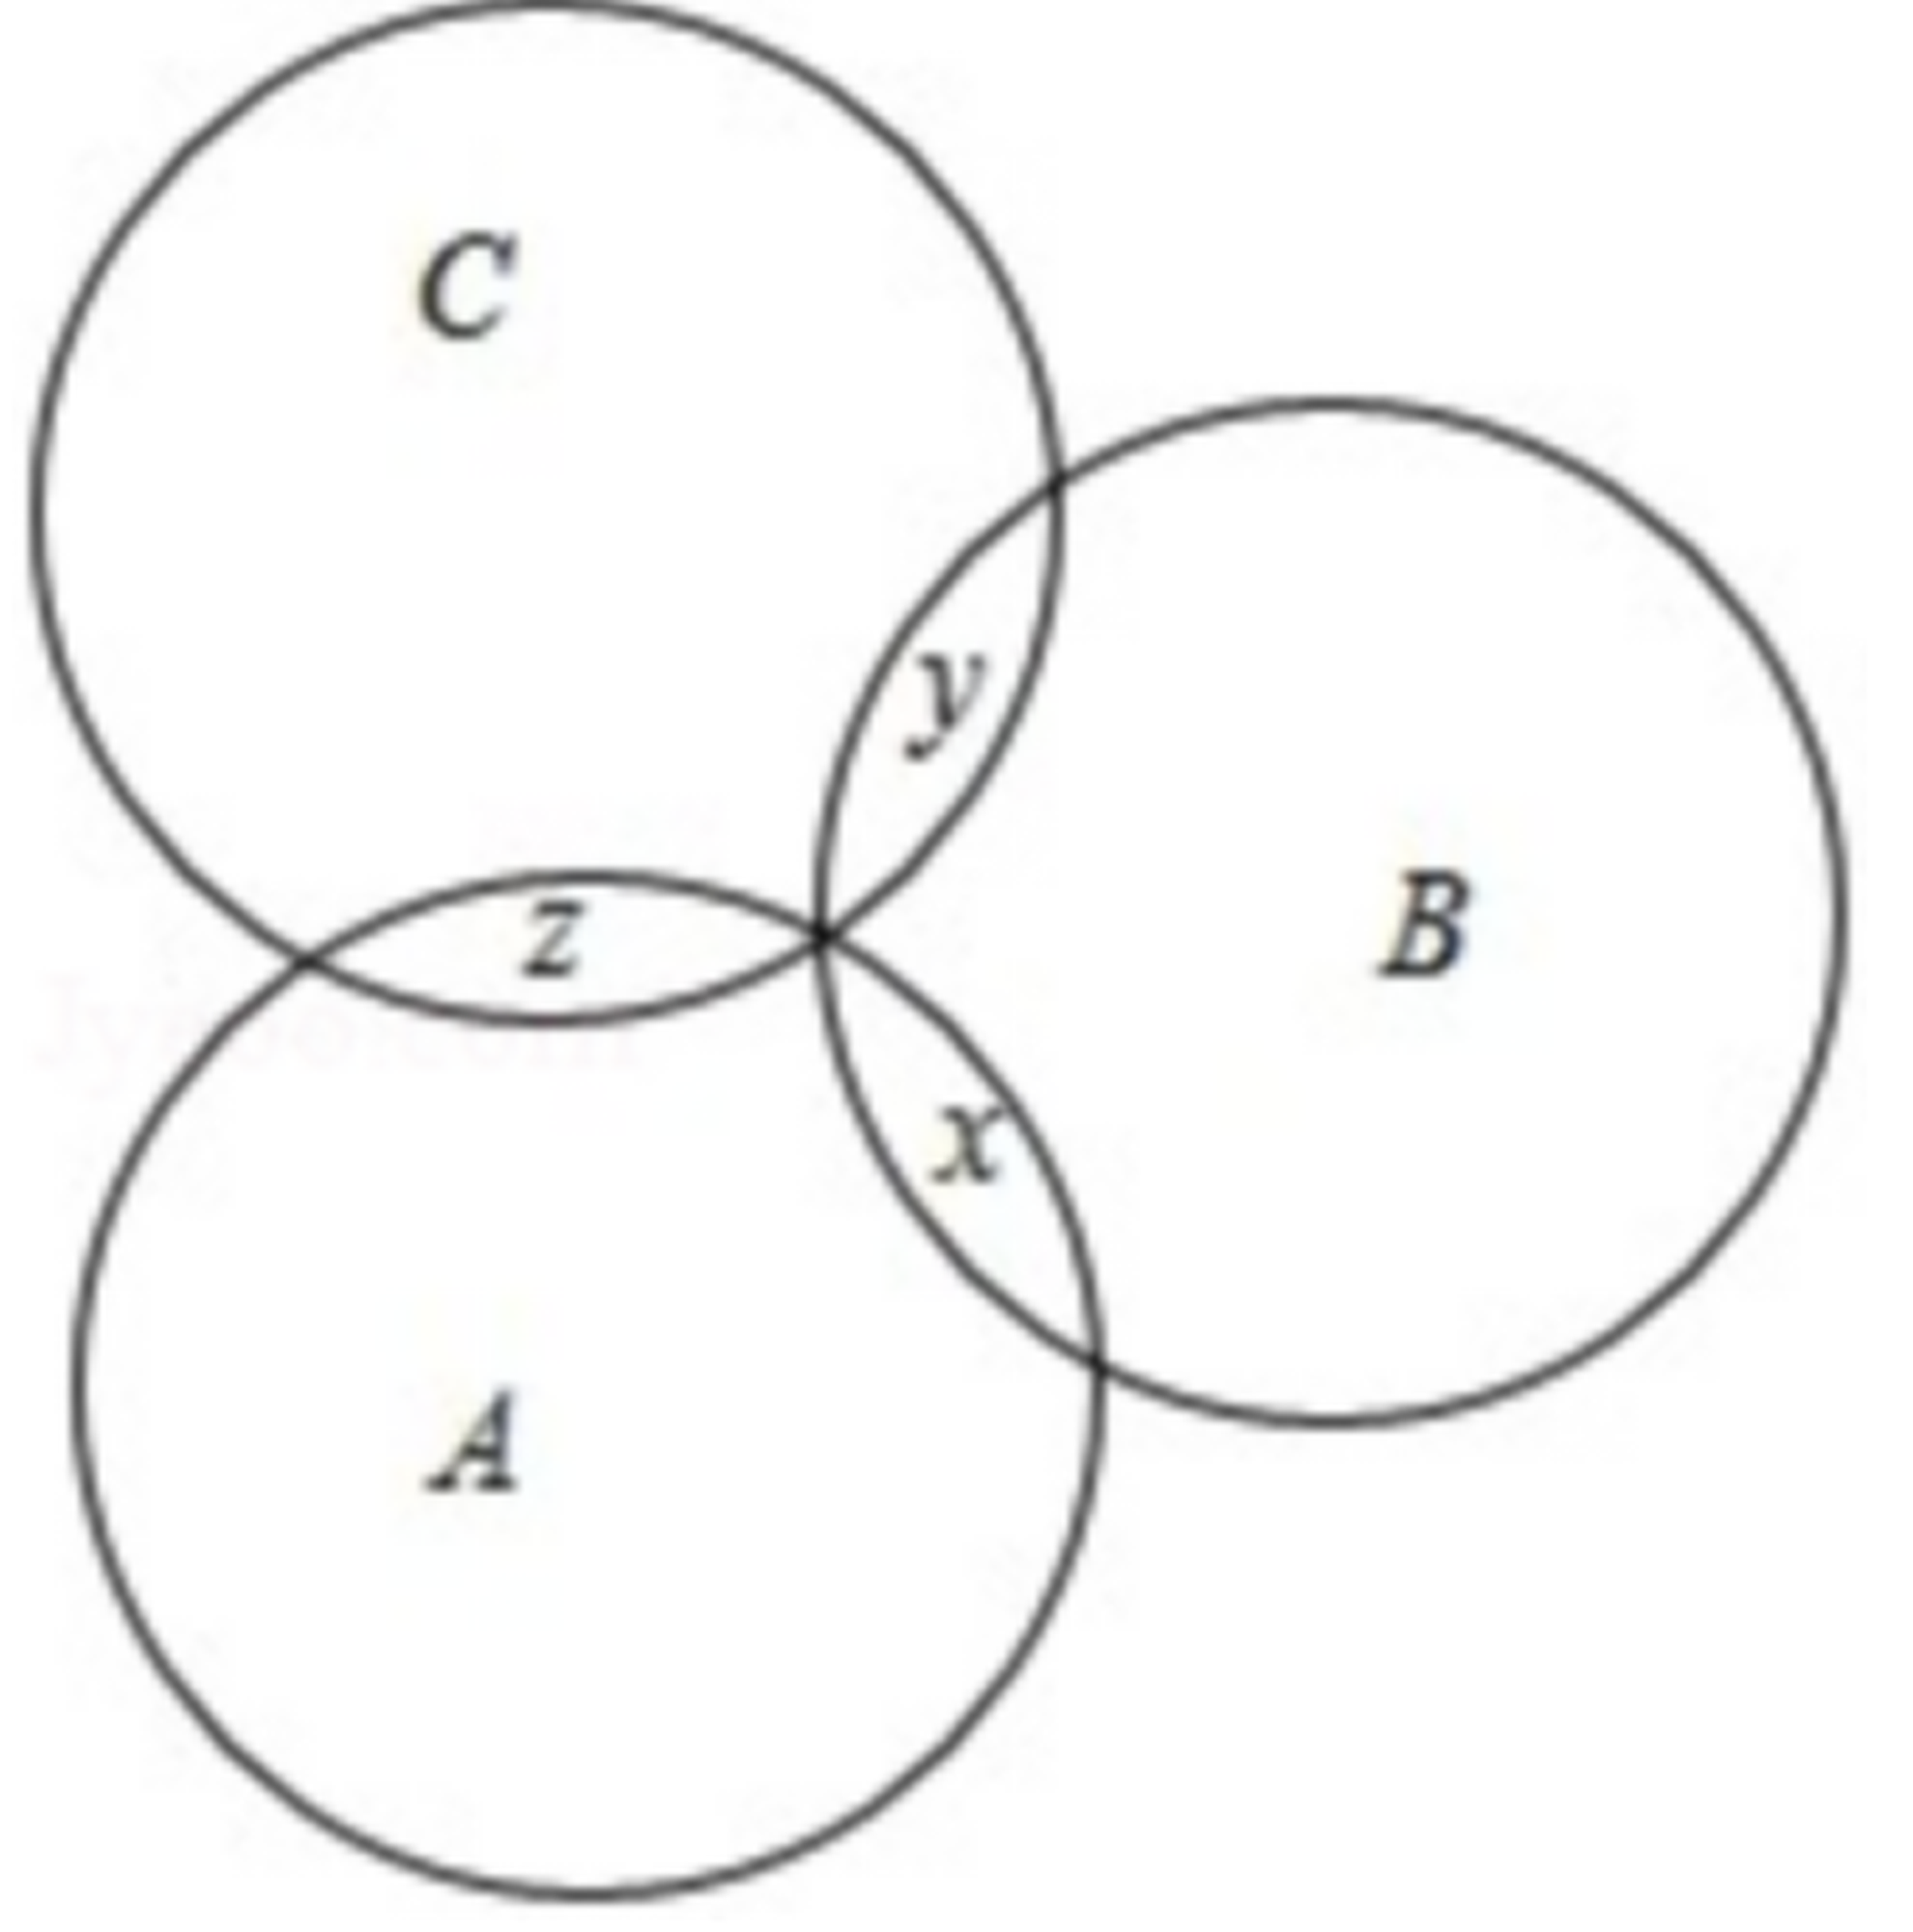
\includegraphics[width=0.30\textwidth]{figures/venn_ABC_x_y_z_h39.png}
\end{center}
\step{因为 $|A\cap B|=|B\cap C|=|C\cap A|=1$，且 $x$、$y$、$z\in\{1,2,3\}$，}
\step{所以集合 $A=\{x,z\}$，$B=\{x,y\}$，$C=\{z,y\}$，}
\step{若 $x=1$，$y=2$，$z=3$，则 $A=\{1,3\}$，$B=\{1,3\}$，$C=\{2,3\}$，}
\step{将 $1$，$2$，$3$ 进行全排列，有 $P_3^3=3\times2=6$ 个.}
\solend

\fi

\item 已知集合 $T=\{1,2,\cdots,2025\}$，对于 $T$ 的每一个非空子集的所有元素，计算它们乘积的倒数，
则所有这样倒数的和为 \blankline[4.4em].

\ans{$2025$}

\ifanswer
\solbegin
\step{集合 $T=\{1,2,\cdots,2025\}$ 的非空子集的个数为 $2^{2025}-1$，}
\step{这些子集中，每个元素的乘积分别为}
\step{$1,2,3,\cdots,2025,1\times2,1\times3,\cdots,1\times2025,\cdots,1\times2\times3\times\cdots\times2025$，}
\step{每项都可以看作是从 $1,2,3,\cdots,2025$ 中选择若干项的乘积，}
\step{$1+\dfrac12+\cdots+\dfrac{1}{2025}+\dfrac{1}{1\times2}+\dfrac{1}{1\times3}+\cdots+\dfrac{1}{2024\times2025}
+\cdots+\dfrac{1}{1\times2\times\cdots\times2025}$}
\step{$=(1+1)\left(1+\dfrac12\right)\cdots\left(1+\dfrac{1}{2025}\right)-1
=2\times\dfrac32\times\dfrac43\times\cdots\times\dfrac{2026}{2025}-1=2025$.}
\solend

\fi

% 第 24 题是压轴题，题干较长；试卷版在它之前量一次页高，尽量不与前文分家（照全稿成例）。
\ansneed{5cm}
% 注：原卷【解析】①③ 两步把 $f(x)$ 印作 $f[x[x]]$，显系笔误，照录未改，见文件头「笔误/存疑」⑦。
\item 若 $X$ 是一个集合，$T$ 是一个以 $X$ 的某些子集为元素的集合，且满足：①$X$ 属于 $T$，
$\varnothing$ 属于 $T$；②$T$ 中任意多个元素的并集属于 $T$；③$T$ 中任意多个元素的交集属于 $T$.
则称 $T$ 是集合 $X$ 上的一个拓扑. 已知函数 $f(x)=[x[x]]$，其中 $[x]$ 表示不大于 $x$ 的最大整数，
当 $x\in(0,n]$，$n\in\N^*$ 时，函数 $f(x)$ 值域为集合 $A_n$，则集合 $A_2$ 上的含有 $4$ 个元素的
拓扑 $T$ 的个数为 \blankline[4.4em].

\ans{$9$}

\ifanswer
\solbegin
\step{由题意，$n=2$，故 $0<x\leqslant2$，}
\step{①当 $0<x<1$ 时，则 $[x]=0$，所以 $f[x[x]]=0$，}
\step{②当 $x=1$ 时，$[x]=1$ 显然 $f(1)=1$，}
\step{③当 $1<x<2$ 时，$[x]=1$，所以 $f[x[x]]=[x]=1$，}
\step{④当 $x=2$ 时，$f(2)=4$，}
\step{所以 $A_2=\{0,1,4\}$，}
\step{因为 $T$ 中含有 $4$ 个元素，其中两个元素 $\varnothing$ 和 $A_2$，}
\step{$A_2=\{0,1,4\}$. 其它两个元素为 $A$、$B$，则
$\begin{cases}A\neq\varnothing\\ A\neq A_2\\ B\neq\varnothing\\ B\neq A_2\\ A\neq B\end{cases}$，}
\step{由对称性，不妨设 $1\leqslant|A|\leqslant|B|\leqslant2$，其中 $|A|$、$|B|$ 表示集合 $A$ 中元素的个数，}
\step{因为 $\begin{cases}A\cap B\in T\\ A\cup B\in T\end{cases}$，又 $|A|\leqslant|B|$，所以 $A\cap B=\varnothing$ 或 $A$，}
\step{若 $A\cap B=\varnothing$，则 $A\cup B$ 只能等于 $A_2$，}
\step{（若 $A\cup B=B$，则 $A\sub B$，则 $A\cap B=A=\varnothing$，矛盾）}
\step{则必有 $\begin{cases}|A|=1\\ |B|=2\end{cases}$，所以 $(A,B)$ 的个数 $\Leftrightarrow$ $A$ 的个数 $=3$ 种，}
\step{即 $\begin{cases}A=\{0\}\\ B=\{1,4\}\end{cases}$ 或 $\begin{cases}A=\{1\}\\ B=\{0,4\}\end{cases}$
或 $\begin{cases}A=\{4\}\\ B=\{0,1\}\end{cases}$；}
\step{若 $A\cap B=A\Leftrightarrow A\sub B$ 此时满足 $A\cup B=B$，}
\step{因为 $A\neq B$ 且 $1\leqslant|A|$ 且 $|B|\leqslant2$，所以 $\begin{cases}|A|=1\\ |B|=2\end{cases}$，}
\step{所以 $B$ 的选择共有 $C_3^2=3$ 种，则 $A$ 的个数有 $C_2^1$ 种，}
\step{所以 $(A,B)$ 的个数 $=2\times3=6$ 种.}
% 这六组「$A$／$B$」按原卷排作两行（前五个一行、第六个另起一行）；因五组并排时
% amsmath 的 cases 会为每组的第二列各留一枚 \quad，本行改排 \left\{\begin{matrix}…\end{matrix}\right.
% 以省下这枚 \quad（照 README「说明」记的高一07 成例），字形与 cases 相同。
\step{（这 $6$ 种是 $\left\{\begin{matrix}A=\{0\}\\ B=\{0,1\}\end{matrix}\right.$、
$\left\{\begin{matrix}A=\{1\}\\ B=\{0,1\}\end{matrix}\right.$、
$\left\{\begin{matrix}A=\{0\}\\ B=\{0,4\}\end{matrix}\right.$、
$\left\{\begin{matrix}A=\{4\}\\ B=\{0,4\}\end{matrix}\right.$、
$\left\{\begin{matrix}A=\{1\}\\ B=\{1,4\}\end{matrix}\right.$、}
\step{$\left\{\begin{matrix}A=\{4\}\\ B=\{1,4\}\end{matrix}\right.$）.}
\step{综上，$T$ 的个数为 $9$ 个.}
\solend

\fi

\end{enumerate}

\end{document}
"
%
% 原始材料是微信公众号图文（公众号「魔都数学加油站」连载「27学年高一 39」，署名「破晓」，
% 2026-09-26 21:29 发布，原文标题「27学年高一39——2026-2027年上海市大同中学高一上周末作业4.1」，
% 原文链接 https://mp.weixin.qq.com/s/HR2hIayXUXNi4zTs3PioiQ ），正文为 11 张 PNG 页。**同一篇里各页分辨率不一致**（2560×3620 与 4762×6735 两档混排：第 1、3、8、10 页为
% 2560×3620，第 2、4、5、6、7、9、11 页为 4762×6735）。原文本身就是一份**讲评版**——除第 15 题
% 外各题题下直接印【解析】（无单独的【答案】行），第 15 题的答案「D」直接印在题干末尾的括号内。
% 试题文字、答案与解析均照原卷录入，未改内容。卷面的粉色斜水印「魔都数学加油站」属水印，未录入。
%
% 卷首标题：原卷页首印作「2026-2027 年大同中学高一上周末作业 4.1」（**卷面标题行即带校名**，
% 年份区间按全稿惯例排 en dash，前缀照原卷保留「年」）。
%
% 篇幅与题号：卷面自「一、填空题」的**第 3 题**起编，终于「附加题」的**第 24 题**，共 22 题
% （填空 3—12、选择 13—16、解答 17—20、附加题 21—24）。第 1、2 题未在该文中发布——这是该
% 公众号连载讲评版的通例（高一02—高一09 等均自第 3 题起编，README「说明」已记），**不是截断**，
% 故本稿题号亦自 3 起。它与 高一40（大同中学 周末作业4.2）同属「周末作业 4」系列但**各自独立起编**
% （4.2 自第 3 题起、终于第 19 题），不是同一份试卷的两半。
%
% 与原卷的排版差异（均已在 README「说明」中交代）：
%   ① 原文自**第 3 题**起（第 1、2 题未在该文中发布），故本稿题号亦自 3 起，填空题以
%      \setcounter{enumi}{2} 起编；选择、解答、附加题三节各按上一节末号另设 \setcounter
%      （选择题 \setcounter{enumi}{12}、解答题 \setcounter{enumi}{16}、附加题 \setcounter{enumi}{20}）；
%   ② 原卷本就印有「一、填空题」「二、选择题」「三、解答题」三节标题，末节印作「附加题」
%      （**不带「四、」**，且题号 21—24 续前编、不另起），本稿照原卷分节，只把标题改排成全稿
%      统一的「大节标题」样式；
%   ③ 原卷是「讲评版」：除第 15 题外，各题题下均印【解析】（**全卷无一条独立的【答案】行**）；
%      第 15 题无解析，答案「D」直接印在题干末尾的括号内。本稿统一改为试卷版隐去、答案版以
%      \ans{}／\ifanswer 块给出，两版彻底分离；原卷写在【解析】末句的结果，本稿照 高一38
%      （同校同系列、同为讲评版）的成例另提为 \ans{}；
%   ④ 数集记号原卷两套并用：实数集作斜体的 $R$（第 7、11、14、17、18、19 题），整数集作斜体
%      $Z$（第 10 题），自然数集作斜体 $N$ 及 $N^*$（第 16、20、21、24 题），本稿按全稿惯例
%      统一写作 $\R$、$\Z$、$\N$、$\N^*$；
%   ⑤ 补集符号原卷两套并用：第 7 题作前缀式的 $C_U$（且题干称全集为 $I$，见「笔误/存疑」①），
%      第 14、15、18 题作上横线（$\overline{H}$、$\overline{A}$、$\overline{B}$），本稿照录、不归一
%      （前缀式写作 $\complement_U$，与 高一c／高一10 的成例一致）；
%   ⑥ 包含符号原卷两套并用：第 3 题作**无下划线**的 $\subset$，第 15、18、20、24 题作**带下划线**
%      的 $\sub$，本稿照录、不归一；
%   ⑦ 原卷填空的横线约两个字宽，本稿按全稿惯例统一排 \blankline[4.4em]；
%   ⑧ 第 7、11、22 题各有插图，取原卷截图、4× LANCZOS 放大（figures/venn_N_cap_CI_M_h39.png、
%      figures/plane_grid_4squares_h39.png、figures/venn_ABC_x_y_z_h39.png）；第 7 题的 Venn 属
%      **题干**（试卷版、答案版都出），第 11、22 题的图在【解析】内（仅答案版出）。第 7 题图
%      左下、第 11 题图的上／左／右边缘带进极淡的原卷粉色水印残影——照全稿「插图直接取自
%      原卷截图、不用 TikZ 重绘、不修图」的体例保留（再裁会切到坐标轴与 $x$、$y$、$O$ 标注）；
%   ⑨ 原卷并列的字母、数字（「$x_1,x_2$」「$a,b$」「$1,2,3,\cdots,11$」）多作半角逗号或不加标点，
%      本稿按全稿惯例改排顿号（$x_1$、$x_2$）或把数列并入行内公式；半角括号、逗号一律排全角，
%      数学式内部的标点照原样；
%   ⑩ 原卷未印副标题，本稿按**本卷实际内容**补出副标题「集合与常用逻辑用语」（依据见下条）。
%
% 副标题（\examtitlest 第二个参数）：本卷卷面未印副标题，由本稿补出，取值按 2026-09-26 起的
%   新口径「只用本卷实际内容的模块名」定为「集合与常用逻辑用语」。依据：全卷 22 题（第 3—24 题）中，
%   第 3、5、7、8、10、11、14、15、16、17、18、19、20、21、22、23、24 题共 17 题是集合的运算与
%   关系、子集／真子集、补集、集合新定义（「全食／偏食」、最小相交、拓扑、特征数）与集合计数，
%   以及命题与常用逻辑用语（第 3 题充要条件、第 5 题存在量词命题、第 17 题命题真假）；其余两题
%   第 4、6 考一元二次方程的根（韦达定理）与方程恒等，第 9、12、13 题是不等式（一元二次不等式组
%   的整数解、一元二次不等式解集、不等式的性质）——不等式合计 3/22，**不足全卷三分之一**，
%   故不并标「不等式」。
%
% 原卷笔误/存疑（均照抄原卷、未改，见源码中该处上方注释）：
%   ① 第 7 题题干称「全集 $I=R$」，而【解析】两处把补集写作 $C_U M$（下标作 $U$），前后记号不一；
%      本稿照录，未改；
%   ② 第 4 题【解析】两处把判别式印作 $\triangle=[2(m-1)^2-16m^2]$（方括号内首项漏了平方，
%      正确应作 $[2(m-1)]^2-16m^2$）；按其所判「$m=\frac12$ 时 $<0$、$m=-\frac12$ 时 $>0$」反推，
%      $[2(m-1)]^2-16m^2$ 在 $m=\frac12$ 时为 $-3<0$、在 $m=-\frac12$ 时为 $5>0$，与结论一致；
%      本稿照录；
%   ③ 第 9 题【解析】把方程组第二式印作 $1-2<-k\leqslant3$，按其结论 $-3\leqslant k<2$ 反推，
%      疑当作 $-2<-k\leqslant3$（原卷多一个「$1$」）；本稿照录；
%   ④ 第 17 题【解析】首句「由数 $y=-x^2+ax-1=-x+3$」中的「由数」显系「由」或「由函数」之误；
%      且末段「若 $p$ 真 $q$ 假…得 $a\in R$」「若 $p$ 假 $q$ 真…此时 $a$ 无解」与结论「$a$ 的取值范围
%      是 $R$」自相矛盾（按 $p:a\leqslant-5$、$q:a>-6$，$p$ 真 $q$ 假应为 $a\leqslant-6$，$p$ 假 $q$ 真
%      应为 $a>-5$，合起来是 $a\leqslant-6$ 或 $a>-5$，并非 $R$）；本稿一律照录，未按正确解法改写；
%   ⑤ 第 18 题【解析】(2) 把 $B=\{x\mid x^2+a\leqslant0\}$（$a<0$）印作右端开的
%      $\{x\mid-\sqrt{-a}\leqslant x<\sqrt{-a}\}$（应为闭的「$\leqslant$」）；按其所判
%      $\sqrt{-a}<\frac12$ 反推，不影响结论；本稿照录；
%   ⑥ 第 22 题【解析】在 $x=1$、$y=2$、$z=3$ 时把 $B=\{x,y\}$ 印作 $\{1,3\}$（应为 $\{1,2\}$），
%      与本行前面「$B=\{x,y\}$」不合；本稿照录；
%   ⑦ 第 24 题【解析】①③ 两步把 $f(x)$ 印作 $f[x[x]]$，显系笔误；本稿照录。
%   ⑧ 第 8 题【解析】「即方程 $x^2+ax+b=x$，$x^2+(a-1)x+b=0$ **由**两个相等的实数根为 $4$」——
%      「由」当为「有」（「设…是…有」的杂糅）；本稿照录；
%   ⑨ 第 10 题：题设 $a\oplus b=b(a^2+b^2+1)$，而集合定义里含 $\dfrac{a\oplus b}{2b}$；$-2<a<b<2$、
%      $a$、$b\in\Z$ 时 $(a,b)=(-1,0)$ 也合条件、却使分母 $2b=0$，原卷解析仍代入该组并约去
%      $b$ 得 $x=1$（答案集恰好不变）；本稿照录；
%   ⑩ 第 15 题选项列里 ② 与 ③ 之间**漏排分隔号**（原卷作「② $\overline{A}\cap B=\varnothing$③
%      $\overline{A}\sub\overline{B}$；」——①、③ 后都有「；」，② 后没有）；本稿照录；
%   ⑪ 第 20(2) 把 $\{1,2,\cdots,20\}$ 分成的 11 个集合里，$\{8,11\}$ 与 $\{9,12\}$ 之间误用
%      **句号**「.」（同行其余处皆逗号）；本稿照录；
%   ⑫ 第 20(3)① 推理不严：原卷写「选 5 则不选 1、9；选 6 则不选 2、10；选 7 则不选 3、11；
%      则只剩 4、8」——但 4 与 8 相差 $4$、不能同选，该情形实际最多只能取 $4$ 个；末句结论
%      「不超过 $5$ 个」仍成立；本稿照录；
%   ⑬ 第 16 题【解析】两种下标并存：「所以在 $A_i$ 的特征数构成中」原卷作斜体 $A_i$，而
%      「要使 $X_1+X_2+X_3$ 最大（小），则（应）在集合 $A_1$ 中首先放置…」两处原卷作
%      **数字 $1$**（与同句 $X_1$ 的角标同形）；本稿照录、未归一。
%
% 图取原卷截图（依次见各处的 \includegraphics 前的注释），4× LANCZOS 放大。
\documentclass[a4paper,11pt]{article}
\usepackage{common}

\begin{document}

\examtitlest[3]{2026--2027 年大同中学高一上周末作业 4.1}{集合与常用逻辑用语}

\bigsec{一、填空题}

\begin{enumerate}
\setcounter{enumi}{2}

\item “$x\geqslant a$”是“$0<x<2$”的必要非充分条件，则实数 $a$ 的取值范围是 \blankline[4.4em].

\ans{$(-\infty,0]$}

\ifanswer
\solbegin
\step{因为 $x\geqslant a$ 是 $0<x<2$ 的必要非充分条件，所以 $(0,2)\subset[a,+\infty)$，所以 $a\leqslant0$，}
\step{则实数 $a$ 的取值范围是 $(-\infty,0]$.}
\solend

\fi

% 注：原卷$[2(m-1)^2-16m^2]$ 首项漏了平方（应为 $[2(m-1)]^2-16m^2$），照录未改，见文件头「笔误/存疑」②。
\item 若关于 $x$ 的方程 $x^2+2(m-1)x+4m^2=0$ 有两个实数根，且这两根互为倒数，则 $m=$ \blankline[4.4em].

\ans{$-\dfrac12$}

\ifanswer
\solbegin
\step{设 $x_1$、$x_2$ 是方程 $x^2+2(m-1)x+4m^2=0$ 有两个实数根，}
\step{则 $x_1x_2=4m^2=1$，解得 $m=\dfrac12$ 或 $m=-\dfrac12$，}
\step{又当 $m=\dfrac12$ 时，$\triangle=[2(m-1)^2-16m^2]<0$，舍去，}
\step{当 $m=-\dfrac12$ 时，$\triangle=[2(m-1)^2-16m^2]>0$，故 $m=-\dfrac12$.}
\solend

\fi

\item 已知命题：“存在 $x\in[1,2]$，使 $x^2+2x+a\geqslant0$”为真命题，则 $a$ 的取值范围是 \blankline[4.4em].

\ans{$a\geqslant-8$}

\ifanswer
\solbegin
\step{若存在 $x\in[1,2]$，使 $x^2+2x+a\geqslant0$，}
\step{则等价为存在 $x\in[1,2]$，使 $x^2+2x\geqslant-a$，}
\step{当存在 $x\in[1,2]$ 时，设 $y=x^2+2x=(x+1)^2-1$，则 $3\leqslant y\leqslant8$，}
\step{所以要使 $x^2+2x\geqslant-a$，则 $8\geqslant-a$，即 $a\geqslant-8$.}
\solend

\fi

\item 已知方程 $a(3x+2)+b(2x-3)=8x+3$ 有无穷多个解，则 $a:b=$ \blankline[4.4em].

\ans{$30:7$}

\ifanswer
\solbegin
\step{$a(3x+2)+b(2x-3)=(3a+2b)x+2a-3b=8x+3$ 有无穷多个解，}
\step{所以 $\begin{cases}3a+2b=8\\ 2a-3b=3\end{cases}$，解得 $a=\dfrac{30}{13}$，$b=\dfrac{7}{13}$，所以 $a:b=30:7$.}
\solend

\fi

% 注：原卷题干称「全集 $I=R$」，而【解析】两处把补集写作 $C_U M$（下标作 $U$），前后记号不一；
%     照录未改，见文件头「笔误/存疑」①。
\item 已知集合 $M=\{x\mid y=\sqrt{3-x^2}\}$，$N=\{x\mid-3\leqslant x\leqslant1\}$，全集 $I=\R$，
则图中阴影部分表示的集合为 \blankline[4.4em].

% 图取原卷截图（01.png，2560×3620）右栏，4× LANCZOS 放大。
\begin{center}
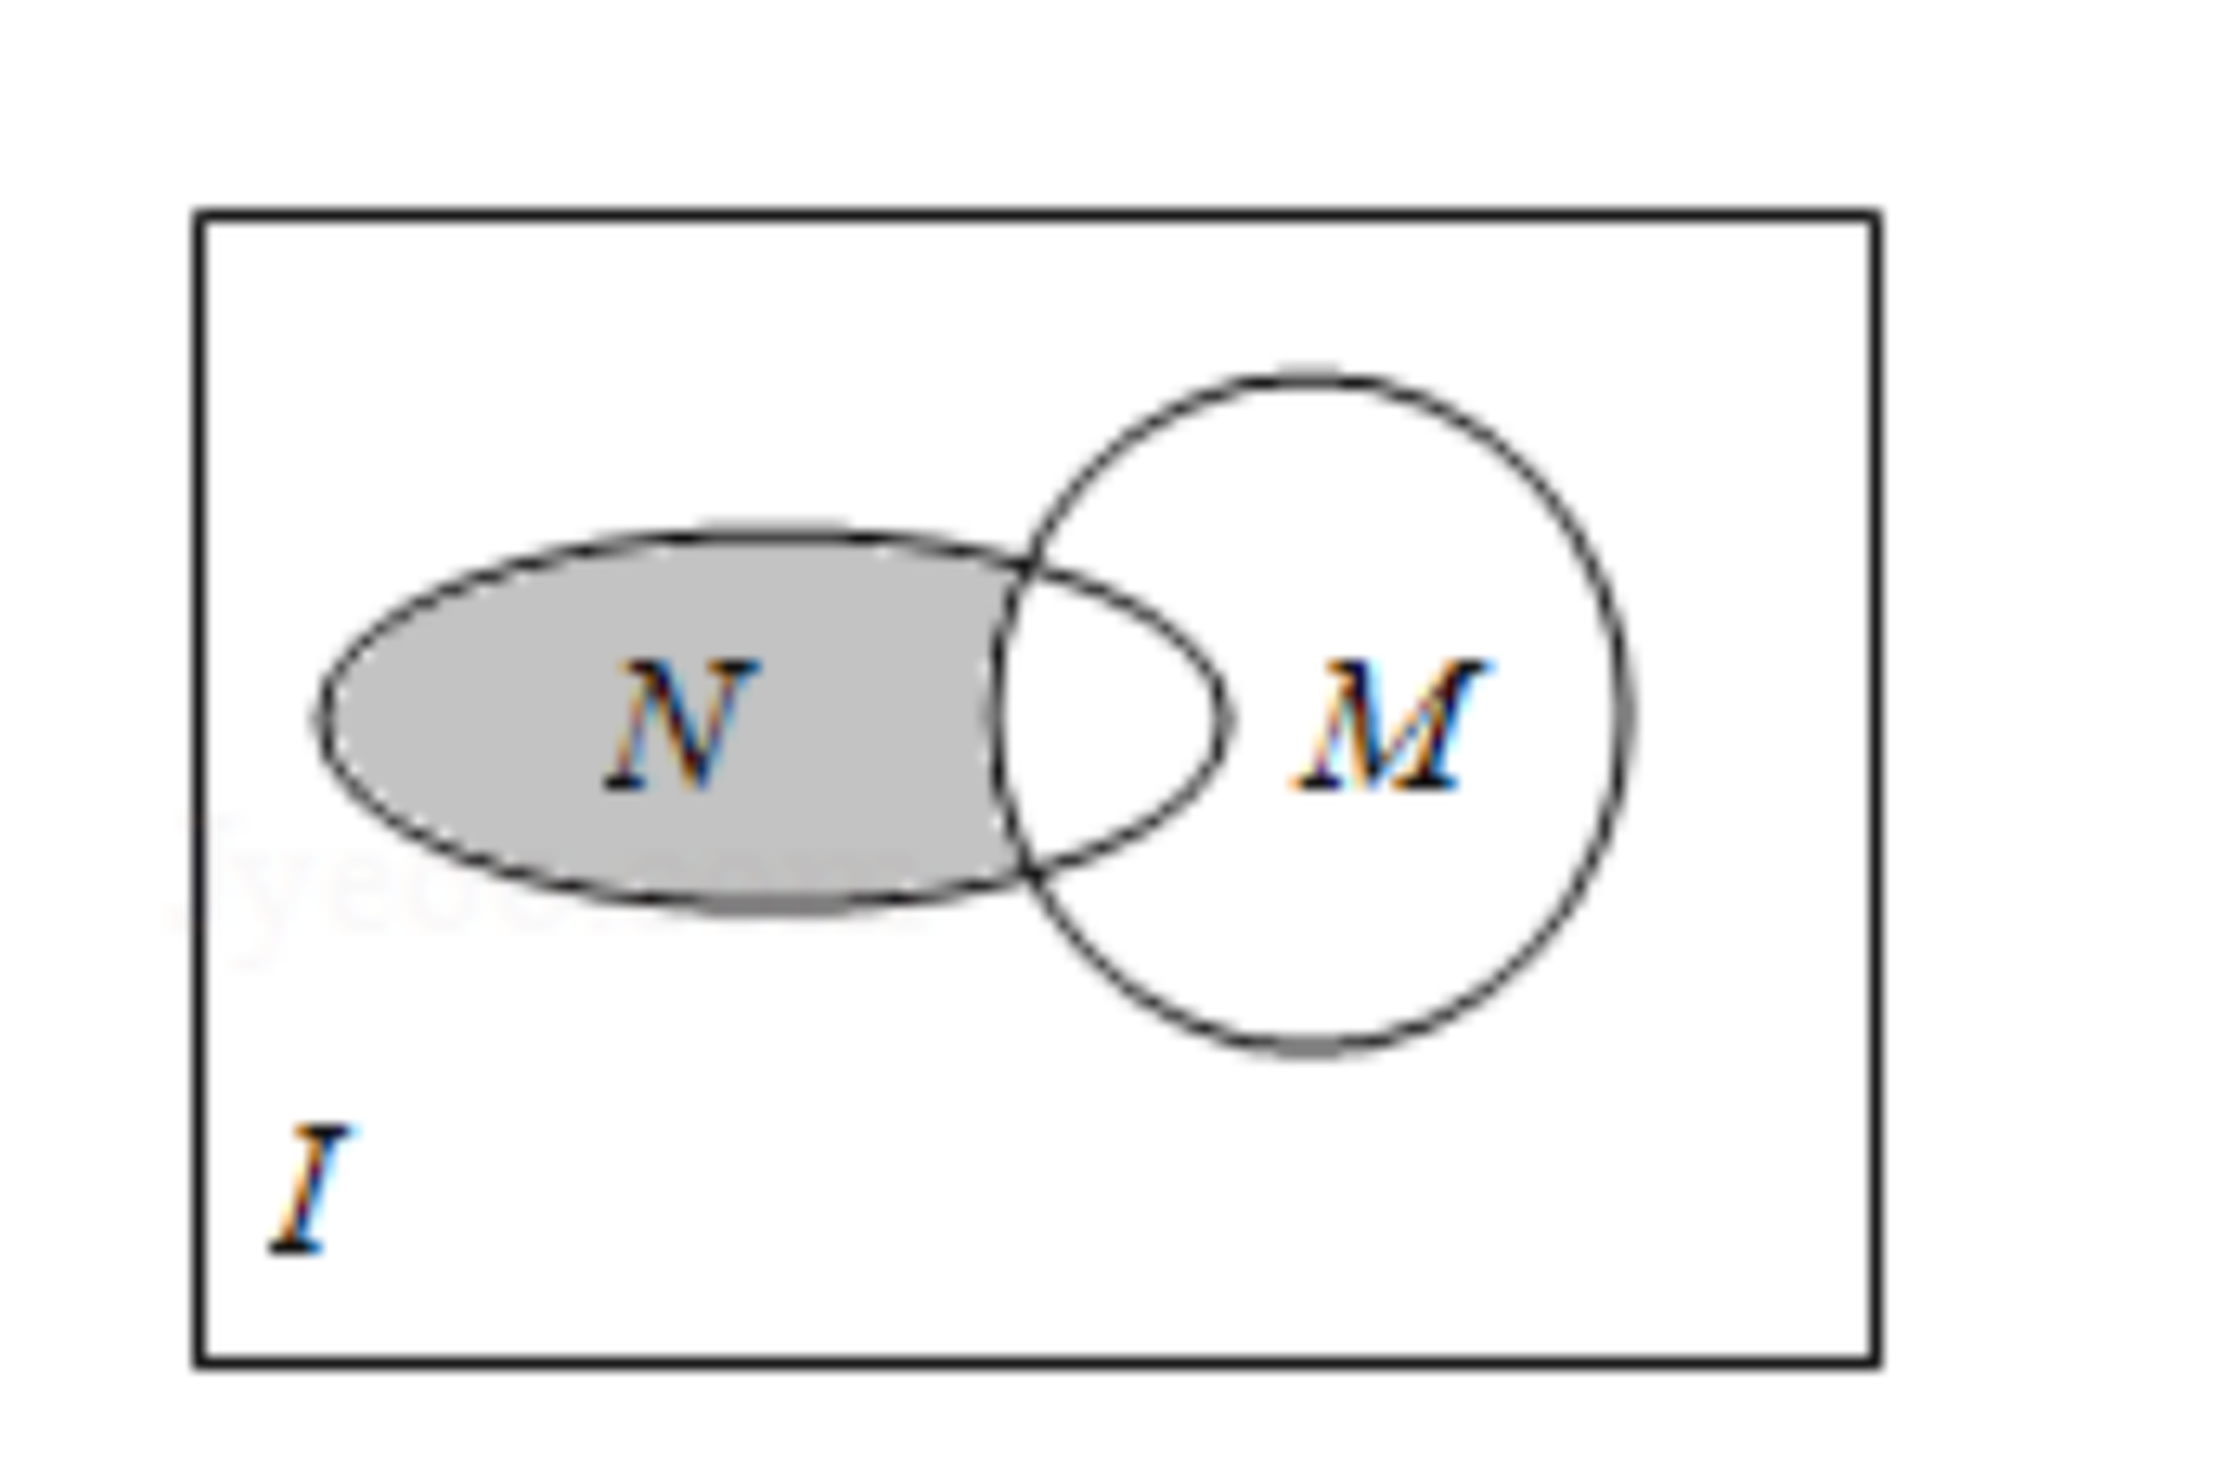
\includegraphics[width=0.30\textwidth]{figures/venn_N_cap_CI_M_h39.png}
\end{center}

\ans{$[-3,-\sqrt3)$}

\ifanswer
\solbegin
\step{阴影部分用集合表示为 $N\cap(\complement_UM)$.}
\step{则 $M=\{x\mid y=\sqrt{3-x^2}\}=\{x\mid3-x^2\geqslant0\}=\{x\mid-\sqrt3\leqslant x\leqslant\sqrt3\}$，}
\step{则 $\complement_UM=\{x\mid x>\sqrt3\text{ 或 }x<-\sqrt3\}$，$N=\{x\mid|x+1|\leqslant2\}=\{x\mid-3\leqslant x\leqslant1\}$，}
\step{则 $N\cap(\complement_UM)=\{x\mid-3\leqslant x<-\sqrt3\}$.}
\solend

\fi

\item 已知 $f(x)=x^2+ax+b$，集合 $\{x\mid f(x)=x\}=\{4\}$，将集合 $M=\{x\mid f(x)=4\}$ 用列举法表示 \blankline[4.4em].

\ans{$\{3,4\}$}

\ifanswer
\solbegin
\step{已知 $f(x)=x^2+ax+b$，集合 $\{x\mid f(x)=x\}=\{4\}$，}
% 注：原卷本行作「…$x^2+(a-1)x+b=0$ **由**两个相等的实数根为 $4$」——「由」当为「有」
%     （「设…是…有」的杂糅）；本稿照录未改，见文件头「原卷笔误/存疑」⑧。
\step{即方程 $x^2+ax+b=x$，$x^2+(a-1)x+b=0$ 由两个相等的实数根为 $4$，}
\step{所以 $\triangle=(a-1)^2-4b=0$，即 $x^2+(a-1)x+b=(x-4)^2$，所以 $b=16$，$a=-7$，}
\step{所以 $f(x)=x^2+ax+b=x^2-7x+16$，所以集合 $M=\{x\mid f(x)=4\}$，}
\step{即 $x^2-7x+16=4$，$x^2-7x+12=0$，故 $M=\{x\mid f(x)=4\}=\{3,4\}$.}
\solend

\fi

% 注：原卷方程组第二式印作 $1-2<-k\leqslant3$，按其结论 $-3\leqslant k<2$ 反推疑当作 $-2<-k\leqslant3$，
%     照录未改，见文件头「笔误/存疑」③。
\item 关于 $x$ 的不等式组 $\begin{cases}x^2-x-2>0\\ 2x^2+(2k+5)x+5k<0\end{cases}$ 的整数解的集合为 $\{-2\}$，
则实数 $k$ 的取值范围 \blankline[4.4em].

\ans{$-3\leqslant k<2$}

\ifanswer
\solbegin
\step{原不等式组即 $\begin{cases}(x-2)(x+1)>0\\ (x+k)(2x+5)<0\end{cases}$，整数解的集合为 $A$，若 $A=\{-2\}$，}
\step{则 $(-2+k)(2\times(-2)+5)<0$，所以 $k<2$，且有 $\begin{cases}-k>-\dfrac52\\ 1-2<-k\leqslant3\end{cases}$，}
\step{解得 $-3\leqslant k<2$.}
\solend

\fi

\item 规定 $\oplus$ 与 $\otimes$ 是两个运算符号，其运算法则如下，对任意实数 $a$、$b$ 有：$a\otimes b=ab$，
$a\oplus b=b(a^2+b^2+1)$. 若 $-2<a<b<2$ 且 $a$、$b\in\Z$，
$A=\left\{x\mid x=2(a\otimes b)+\dfrac{a\oplus b}{2b}\right\}$，则用列举法表示集合 $A=$ \blankline[4.4em].

\ans{$\left\{1,-\dfrac12\right\}$}

\ifanswer
\solbegin
\step{$A=\left\{x\mid x=2(a\otimes b)+\dfrac{a\oplus b}{2b}\right\}
=\left\{x\mid x=2ab+\dfrac{b(a^2+b^2+1)}{2b}\right\}$}
\step{$=\left\{x\mid x=2ab+\dfrac12a^2+\dfrac12b^2+\dfrac12\right\}
=\left\{x\mid x=\dfrac12(a+b)^2+ab+\dfrac12\right\}$，}
% 注：题设含 $\dfrac{a\oplus b}{2b}$，而 $-2<a<b<2$、$a$、$b\in\Z$ 时 $(a,b)=(-1,0)$ 也合条件、
%     却使分母 $2b=0$；原卷解析仍代入该组并约去 $b$ 得 $x=1$（答案集恰好不变）。本稿照录，
%     见文件头「原卷笔误/存疑」⑨。
\step{当 $a=-1$，$b=0$ 时，$x=1$；当 $a=-1$，$b=1$ 时，$x=-\dfrac12$；}
\step{当 $a=0$，$b=1$ 时，$x=1$；所以 $A=\left\{1,-\dfrac12\right\}$.}
\solend

\fi

\item 高斯是德国著名的数学家，近代数学奠基者之一，享有“数学王子”的称号，为了纪念数学家高斯，
我们把取整函数 $y=[x]$，$x\in\R$ 称为高斯函数，其中 $[x]$ 表示不超过 $x$ 的最大整数，
如 $[1.1]=1$，$[-1.1]=-2$. 则点集 $P=\{(x,y)\mid[x]^2+[y]^2=1\}$
所表示的平面区域的面积是 \blankline[4.4em].

\ans{$4$}

\ifanswer
\solbegin
\step{$[x]^2+[y]^2=1$ 由 $\begin{cases}[x]=0\\ [y]=-1\end{cases}$ 或 $\begin{cases}[x]=0\\ [y]=1\end{cases}$
或 $\begin{cases}[x]=-1\\ [y]=0\end{cases}$ 或 $\begin{cases}[x]=1\\ [y]=0\end{cases}$ 四个平面区域组成，}
\step{即 $\begin{cases}0\leqslant x<1\\ -1\leqslant y<0\end{cases}$ 或 $\begin{cases}0\leqslant x<1\\ 1\leqslant y<2\end{cases}$
或 $\begin{cases}-1\leqslant x<0\\ 0\leqslant y<1\end{cases}$ 或 $\begin{cases}1\leqslant x<2\\ 0\leqslant y<1\end{cases}$，}
\step{作出平面区域如图所示，平面区域由四个边长为 $1$ 的正方形组成，}
% 图在【解析】内（仅答案版出），取原卷截图（03.png，2560×3620）中部，4× LANCZOS 放大。
\begin{center}
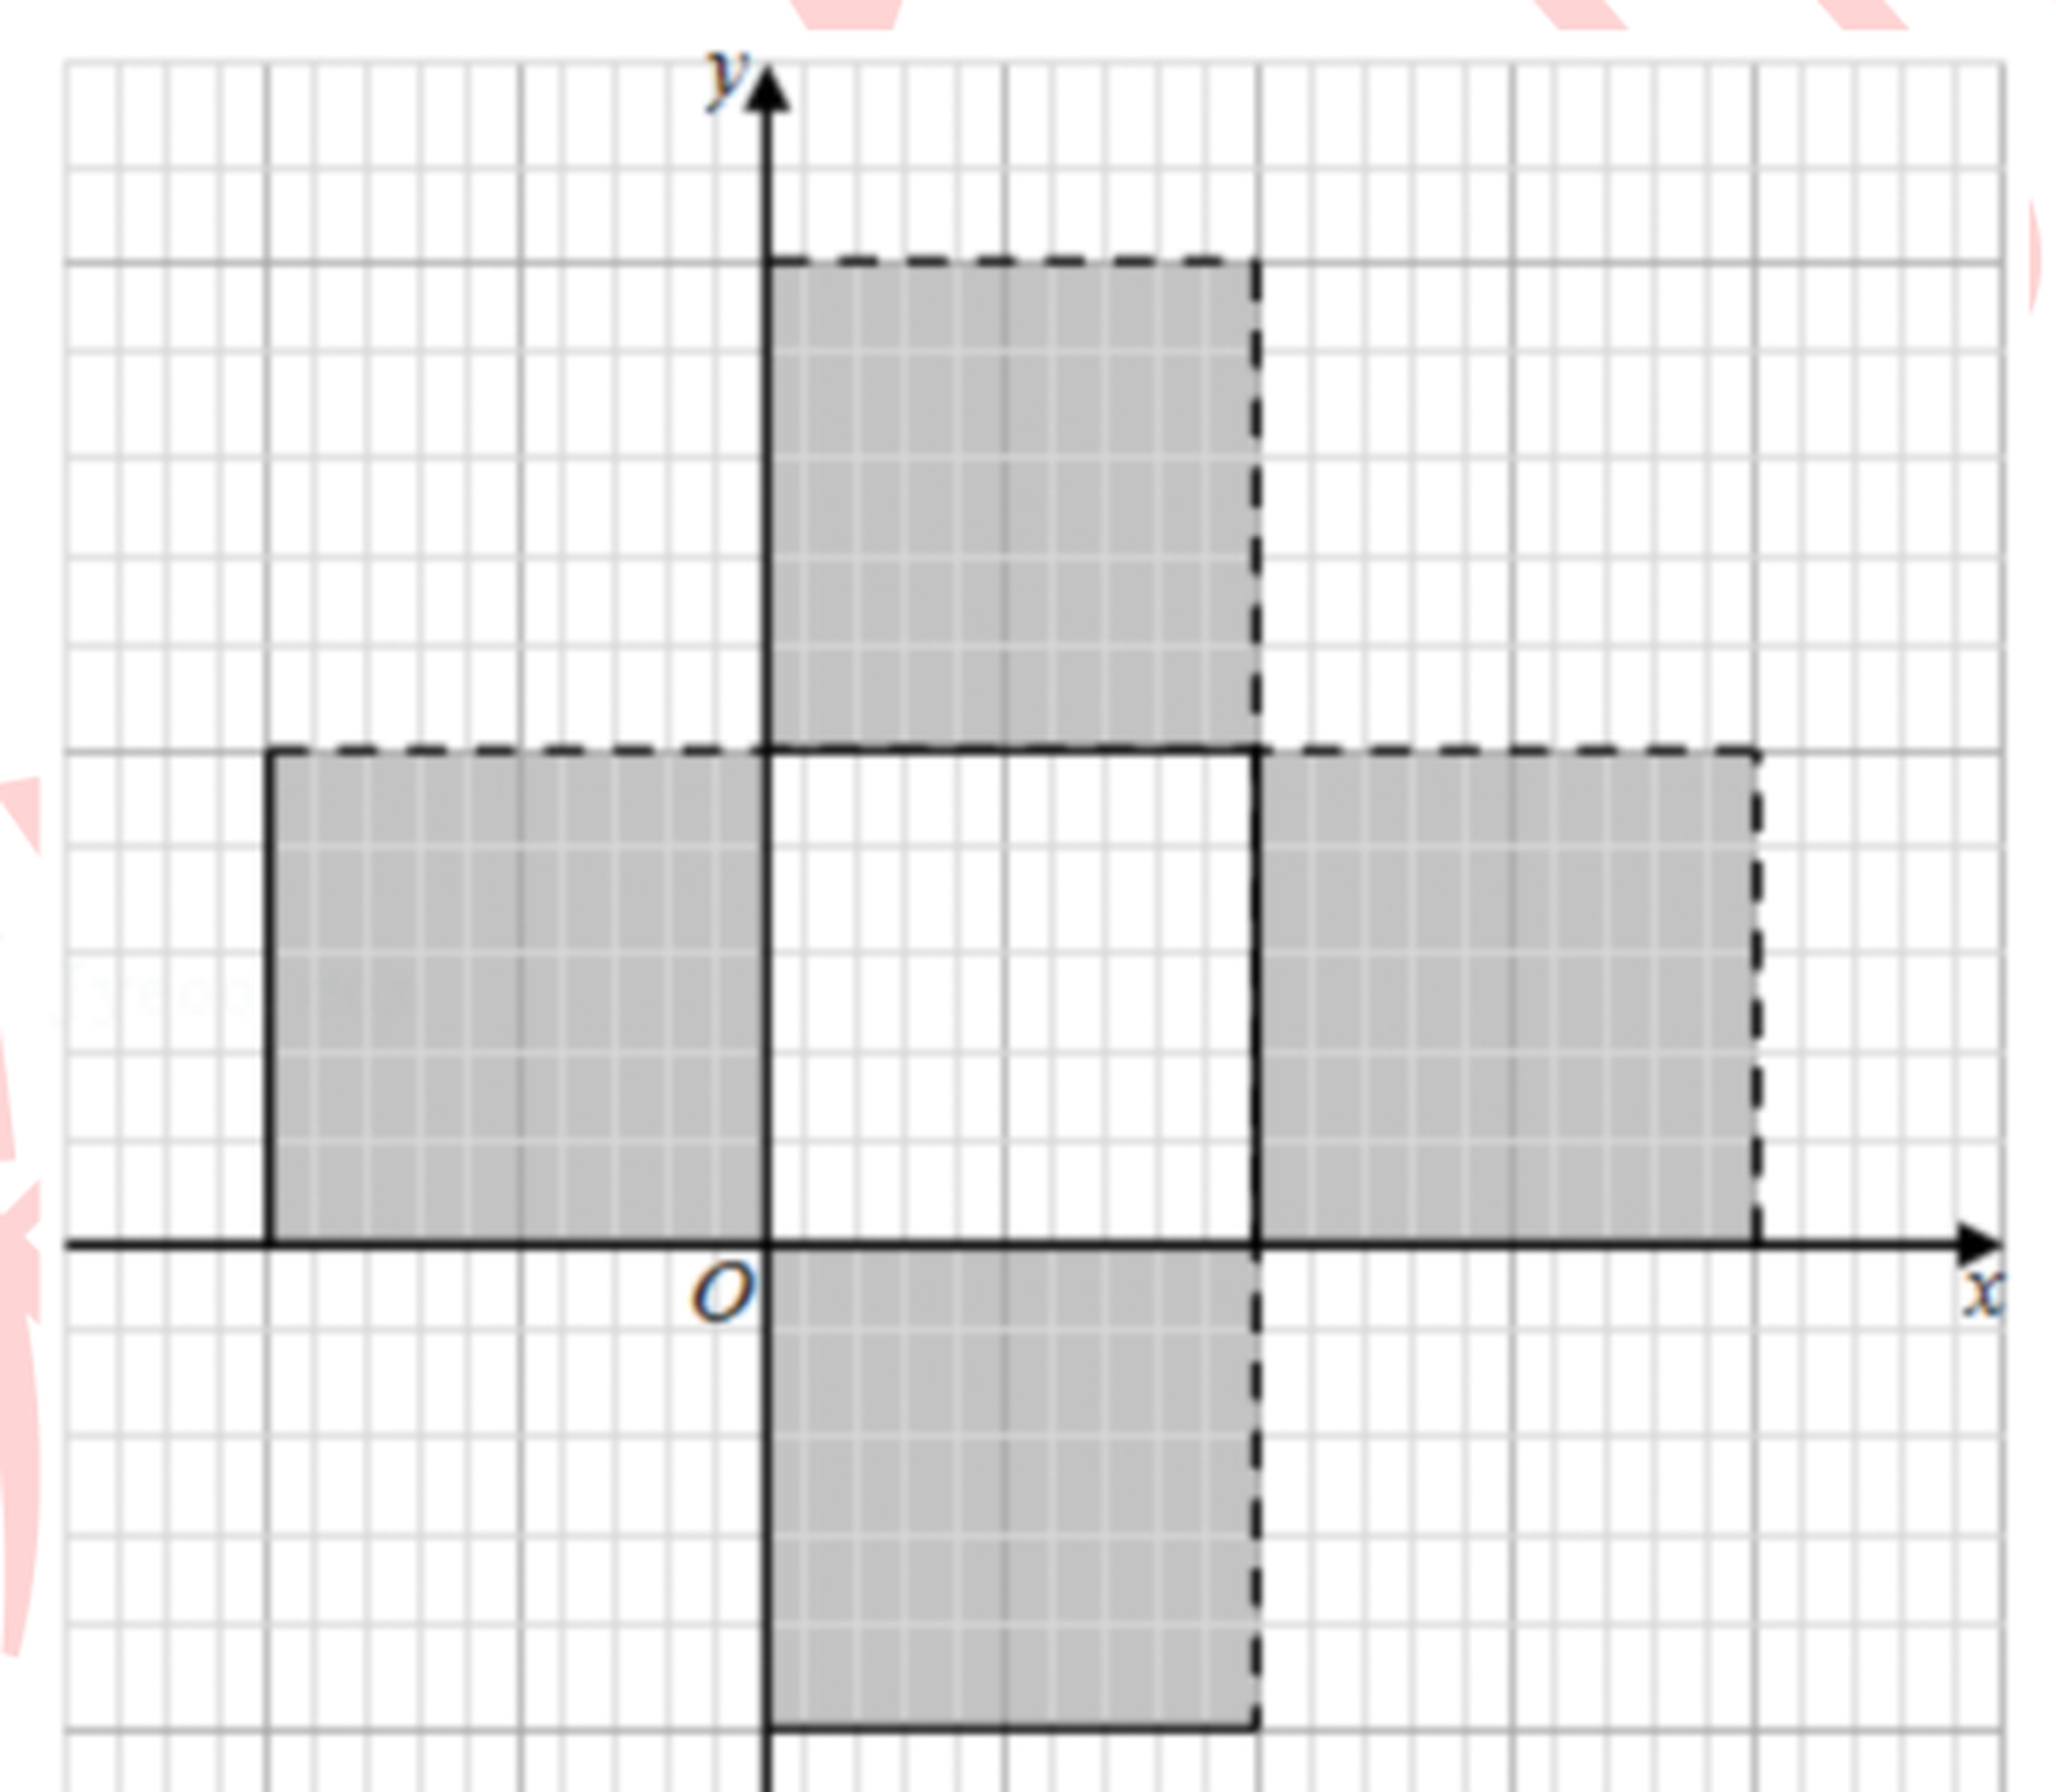
\includegraphics[width=0.38\textwidth]{figures/plane_grid_4squares_h39.png}
\end{center}
\step{总面积为 $1\times4=4$.}
\solend

\fi

\item 关于 $x$ 的不等式 $ax^2+bx+c>0$ 的解集为 $\{x\mid x<\beta\text{ 或 }x>\gamma\}(0<\beta<\gamma)$，
则不等式 $a(x^2+1)+b(x-1)+c>2ax$ 的解集为 \blankline[4.4em].

\ans{$(-\infty,\beta+1)\cup(\gamma+1,+\infty)$}

\ifanswer
\solbegin
\step{由题意得 $\beta$、$\gamma$ 为方程 $ax^2+bx+c=0$ 的两根且 $a>0$，}
\step{则 $\beta+\gamma=-\dfrac ba$，$\beta\gamma=\dfrac ca$，故 $b=-a(\beta+\gamma)$，$c=\beta\gamma a$，}
\step{则不等式可化为 $a(x^2+1)-a(\beta+\gamma)(x-1)+\beta\gamma a>2ax$，}
\step{因为 $a>0$，所以 $x^2+1-(\beta+\gamma)(x-1)+\beta\gamma>2x$，}
\step{即 $x^2-(\beta+\gamma+2)x+(\beta+\gamma+\beta\gamma+1)>0$，所以 $(x-\beta-1)(x-\gamma-1)>0$，}
\step{解得 $x<\beta+1$ 或 $x>\gamma+1$，所以不等式解集为 $(-\infty,\beta+1)\cup(\gamma+1,+\infty)$.}
\solend

\fi

\end{enumerate}

\bigsec{二、选择题}

\begin{enumerate}
\setcounter{enumi}{12}

\item 设 $a<b<0$，则下列不等式中不成立的是\mbox{（\quad）}

\keepwithprev
A. $\dfrac1a>\dfrac1b$\qquad B. $\dfrac{1}{a-b}>\dfrac1a$\qquad C. $|a|>-b$\qquad D. $\sqrt{-a}>\sqrt{-b}$

\ans{$B$}

\ifanswer
\solbegin
\step{令 $a=-2$，$b=-1$，}
\step{A、$-\dfrac12>-1$，正确；B、$-1<-\dfrac12$，故 B 错误；C、$2>1$，正确；}
\step{D、$\sqrt2>1$，正确；故选 B.}
\solend

\fi

\item 设实数集 $\R$ 为全集，集合 $P=\{x\mid f(x)=0\}$，$Q=\{x\mid g(x)=0\}$，$H=\{x\mid h(x)=0\}$，
则方程 $\dfrac{f^2(x)+g^2(x)}{h(x)}=0$ 的解集是\mbox{（\quad）}

\keepwithprev
A. $P\cap Q\cap\overline{H}$\qquad B. $P\cap Q$\qquad C. $P\cap Q\cap H$\qquad D. $P\cap Q\cup H$

\ans{$A$}

\ifanswer
\solbegin
\step{方程 $\dfrac{f^2(x)+g^2(x)}{h(x)}=0$ 等价于 $\begin{cases}f(x)=0\\ g(x)=0\\ h(x)\neq0\end{cases}$，}
\step{又因为 $P=\{x\mid f(x)=0\}$，$Q=\{x\mid g(x)=0\}$，$H=\{x\mid h(x)=0\}$，}
\step{所以方程 $\dfrac{f^2(x)+g^2(x)}{h(x)}=0$ 的解集是 $P\cap Q\cap\overline{H}$，故选 A.}
\solend

\fi

\item 设全集 $U$，在下列条件中，是 $B\sub A$ 的充要条件的有\mbox{（\quad）}

\keepwithprev
% 注：原卷此行 ② 与 ③ 之间**漏排分隔号**（①、③ 后都有「；」，② 后没有）；
%     本稿照录未补，见文件头「原卷笔误/存疑」⑩。
①$A\cup B=A$；\qquad ②$\overline{A}\cap B=\varnothing$\qquad ③$\overline{A}\sub\overline{B}$；\qquad ④$A\cup\overline{B}=U$

\keepwithprev
A. $1$ 个\qquad B. $2$ 个\qquad C. $3$ 个\qquad D. $4$ 个

\ans{$D$}

\item 已知集合 $M=\{x\mid x\in\N,0<x\leqslant15\}$，$A_1$、$A_2$、$A_3$ 满足：①$A_1\cup A_2\cup A_3=M$；
②每个集合都恰有 $5$ 个元素. 集合 $A_i(i=1,2,3)$ 中最大元素与最小元素之和称为 $A_i$ 的特征数，
记为 $X_i(i=1,2,3)$，则 $X_1+X_2+X_3$ 的值不可能为\mbox{（\quad）}

\keepwithprev
A. $37$\qquad B. $39$\qquad C. $48$\qquad D. $57$

\ans{$A$}

\ifanswer
\solbegin
\step{因为集合 $M=\{x\mid x\in\N,0<x\leqslant15\}=\{1,2,3,\cdots,15\}$，}
\step{又因为集合 $A_1$、$A_2$、$A_3$ 中，每个集合恰有 $5$ 个元素，}
\step{且 $A_1\cup A_2\cup A_3=M$ 有 $15$ 个元素，所以集合 $A_1$、$A_2$、$A_3$ 中没有重复元素，}
\step{因为 $1$ 是集合 $M$ 中数值最小的元素，$15$ 是集合 $M$ 中数值最大的元素，}
\step{所以在 $A_i$ 的特征数构成中，必有 $1$ 和 $15$，不妨设 $1\in A_1$，$15\in A_1$，}
% 注：原卷本行（与下面「最小」那句）在「集合」后的角标是**数字 $1$**（同句 $X_1$ 的角标同形），
%     而非上一行「$A_i$ 的特征数构成」里的斜体 $A_i$——原卷两种下标并存，本稿照录、不归一，
%     见文件头「原卷笔误/存疑」⑬。
\step{要使 $X_1+X_2+X_3$ 最大，则应该在集合 $A_1$ 中首先放置数值较小的元素，}
\step{即 $A_1=\{1,2,3,4,15\}$，所以 $5$ 与 $14$ 是剩下元素中数值最小或最大的元素，}
\step{同理，不妨设 $5\in A_2$，$14\in A_2$，接着在 $A_2$ 中再次放置数值较小的元素，}
\step{即 $A_2=\{5,6,7,8,14\}$，则 $A_3=\{9,10,11,12,13\}$，}
\step{此时 $X_1+X_2+X_3$ 有最大值为 $1+15+5+14+9+13=57$，}
\step{即 $X_1+X_2+X_3\leqslant57$；}
% 注：同上一处——原卷此行角标是**数字 $1$**（$A_1$），本稿照录，未与「$A_i$」归一。
\step{要使 $X_1+X_2+X_3$ 最小，则在集合 $A_1$ 中首先放置数值较大的元素，}
\step{即 $A_1=\{1,12,13,14,15\}$，所以 $2$ 与 $11$ 是剩下元素中数值最小或最大的元素，}
\step{同理，不妨设 $2\in A_2$，$11\in A_2$，接着在 $A_2$ 中再次放置数值较大的元素，}
\step{即 $A_2=\{2,8,9,10,11\}$，则 $A_3=\{3,4,5,6,7\}$，}
\step{此时 $X_1+X_2+X_3$ 有最小值为 $1+15+2+11+3+7=39$，}
\step{即 $X_1+X_2+X_3\geqslant39$，}
\step{综上，$39\leqslant X_1+X_2+X_3\leqslant57$，故选 A.}
\solend

\fi

\end{enumerate}

\bigsec{三、解答题}

\begin{enumerate}
\setcounter{enumi}{16}

% 注：原卷首句「由数 $y=-x^2+ax-1=-x+3$」中的「由数」显系「由」或「由函数」之误；末段
%     的两处分类讨论与结论自相矛盾（详见文件头「笔误/存疑」④）。本稿一律照录，未改。
\item 命题 $p$：函数 $y=-x^2+ax-1$ 与 $y=-x+3$ 图象交点的横坐标均为负值，
命题 $q$：关于 $x$ 的方程 $2(1-x)a+(x^2-10x-3)=0$ 的两个根，一个大于 $3$，另一个小于 $3$；
若命题 $p$ 和命题 $q$ 中有且仅有一个是真命题，求 $a$ 的取值范围.

\ans{$\R$}

\ifanswer
\solbegin
\step{由数 $y=-x^2+ax-1=-x+3$ 得 $x^2-(a+1)x+4=0$，}
\step{若横坐标均为负值，则满足 $\begin{cases}\Delta=(a+1)^2-16\geqslant0\\ x_1x_2=4>0\\ x_1+x_2=a+1<0\end{cases}$
得 $\begin{cases}a\geqslant3\text{ 或 }a\leqslant-5\\ a<-1\end{cases}$，得 $a\leqslant-5$，}
\step{即 $p:a\leqslant-5$，}
\step{若方程 $2(1-x)a+(x^2-10x-3)=0$ 的两个根，一个大于 $3$，另一个小于 $3$；}
\step{设 $f(x)=2(1-x)a+(x^2-10x-3)$，则 $f(3)<0$，即 $-4a-24<0$，}
\step{得 $a>-6$，即 $q:a>-6$，}
\step{因为命题 $p$ 和命题 $q$ 中有且仅有一个是真命题，}
\step{若 $p$ 真 $q$ 假，则 $\begin{cases}a\leqslant-5\\ a>-6\end{cases}$，得 $a\in\R$，}
\step{若 $p$ 假 $q$ 真，则 $\begin{cases}a>-5\\ a\leqslant-6\end{cases}$，此时 $a$ 无解，}
\step{综上，实数 $a$ 的取值范围是 $\R$.}
\solend

\fi

\ansspace[8]

\item 设全集是实数集 $\R$，$A=\left\{x\mid\dfrac{1-2x}{x-3}\geqslant0\right\}$，$B=\{x\mid x^2+a\leqslant0\}$.

\begin{enumerate}[label=(\arabic*)]

\item 当 $a=-4$ 时，求 $A\cup B$；

\item 若 $\overline{A}\cap B=B$，求实数 $a$ 的取值范围.

\end{enumerate}

\ans{（1）$\{x\mid-2\leqslant x<3\}$；（2）$\left(-\dfrac14,+\infty\right)$}

\ifanswer
\solbegin
\stepm{(1)}{$A=\left\{x\mid\dfrac{1-2x}{x-3}\geqslant0\right\}=\left\{x\mid\dfrac12\leqslant x<3\right\}$，$B=\{x\mid x^2+a\leqslant0\}$.}
\step{当 $a=-4$ 时，$B=\{x\mid-2\leqslant x\leqslant2\}$，所以 $A\cup B=\{x\mid-2\leqslant x<3\}$.}
\stepm{(2)}{$\overline{A}=\left\{x\mid x\geqslant3\text{ 或 }x<\dfrac12\right\}$，$B=\{x\mid x^2+a\leqslant0\}$.}
\step{由 $\overline{A}\cap B=B$，得 $B\sub\overline{A}$，}
\step{则当 $a>0$ 时，$B=\varnothing$，满足 $B\sub\overline{A}$，则 $a>0$ 成立，}
\step{则当 $a=0$ 时，$B=\{0\}$，满足 $B\sub\overline{A}$，则 $a=0$ 成立，}
\step{当 $a<0$ 时，$B=\{x\mid-\sqrt{-a}\leqslant x<\sqrt{-a}\}$，}
\step{得 $\sqrt{-a}<\dfrac12$，即 $-\dfrac14<a<0$，}
\step{综上，实数 $a$ 的取值范围是 $\left(-\dfrac14,+\infty\right)$.}
\solend

\fi

\ansspace[6]

\item 设集合 $A=\{x\mid ax^2+2x+1=0,a\in\R\}$.

\begin{enumerate}[label=(\arabic*)]

\item 当 $A$ 中元素个数为 $1$ 时，求：$a$ 和 $A$；

\item 当 $A$ 中元素个数至少为 $1$ 时，求：$a$ 的取值范围；

\item 求：$A$ 中各元素之和.

\end{enumerate}

\ans{（1）$a=0$ 时 $A=\left\{-\dfrac12\right\}$，$a=1$ 时 $A=\{-1\}$；（2）$(-\infty,1]$；
（3）$a=0$ 时和为 $-\dfrac12$，$a<1$ 且 $a\neq0$ 时和为 $-\dfrac2a$，$a=1$ 时和为 $-1$，$a>1$ 时 $A$ 中无元素}

\ifanswer
\solbegin
\stepm{(1)}{集合 $A=\{x\mid ax^2+2x+1=0,a\in\R\}$，$A$ 中元素个数为 $1$，}
\step{所以 $a=0$ 或 $\begin{cases}a\neq0\\ \Delta=4-4a=0\end{cases}$，解得 $a=0$，$A=\left\{-\dfrac12\right\}$ 或 $a=1$，$A=\{-1\}$.}
\stepm{(2)}{当 $A$ 中元素个数至少为 $1$ 时，$a=0$ 或 $\begin{cases}a\neq0\\ \Delta=4-4a\geqslant0\end{cases}$，解得 $a\leqslant1$，}
\step{所以 $a$ 的取值范围是 $(-\infty,1]$.}
\stepm{(3)}{当 $a=0$ 时，$A$ 中元素之和为 $-\dfrac12$；}
\step{当 $a<1$ 且 $a\neq0$ 时，$A$ 中元素之和为 $-\dfrac2a$；}
\step{当 $a=1$ 时，$A$ 中元素之和为 $-1$；}
\step{当 $a>1$ 时，$A$ 中无元素.}
\solend

\fi

\ansspace[8]

\item 设 $k$ 是正整数，集合 $A$ 至少有两个元素，且 $A\sub\N^*$. 如果对于 $A$ 中的任意两个不同的
元素 $x$、$y$，都有 $|x-y|\neq k$，则称 $A$ 具有性质 $P(k)$.

\begin{enumerate}[label=(\arabic*)]

\item 试判断集合 $B=\{1,2,3,4\}$ 和 $C=\{1,4,7,10\}$ 是否具有性质 $P(2)$？并说明理由；

\item 若集合 $A=\{a_1,a_2,\cdots,a_{12}\}\sub\{1,2,\cdots,20\}$，求证：$A$ 不可能具有性质 $P(3)$；

\item 若集合 $A\sub\{1,2,\cdots,2023\}$，且同时具有性质 $P(4)$ 和 $P(7)$，求集合 $A$ 中元素个数的
最大值.

\end{enumerate}

\ans{（1）$B$ 不具有性质 $P(2)$，$C$ 具有性质 $P(2)$；（2）见解析；（3）$920$}

\ifanswer
\solbegin
\stepm{(1)}{因为 $B=\{1,2,3,4\}$，}
\step{又 $1\in\N^*$，$2\in\N^*$，$3\in\N^*$，$4\in\N^*$，但 $|4-2|=2$，}
\step{所以集合 $B$ 不具有性质 $P(2)$，}
\step{因为 $C=\{1,4,7,10\}$，}
\step{又 $1\in\N^*$，$4\in\N^*$，$7\in\N^*$，$10\in\N^*$，}
\step{但 $|4-1|=3$，$|7-1|=6$，$|10-1|=9$，$|7-4|=3$，$|10-4|=6$，$|10-7|=3$，}
\step{所以集合 $C$ 具有性质 $P(2)$，}
\stepm{(2)}{将集合 $\{1,2,\cdots,20\}$ 中的元素分为如下 $11$ 个集合，}
% 注：原卷本行 $\{8,11\}$ 与 $\{9,12\}$ 之间的分隔号误用**句号**「.」（同行其余处皆逗号），
%     本稿照录、未改，见文件头「原卷笔误/存疑」⑪。
\step{$\{1,4\}$，$\{2,5\}$，$\{3,6\}$，$\{7,10\}$，$\{8,11\}$.$\{9,12\}$，$\{13,16\}$，$\{14,17\}$，$\{15,18\}$，}
\step{$\{19\}$，$\{20\}$，}
\step{所以从集合 $\{1,2,\cdots,20\}$ 中取 $12$ 个元素，则前 $9$ 个集合至少要选 $10$ 个元素，}
\step{所以必有 $2$ 个元素取自前 $9$ 个集合中的同一集合，即存在两个元素其差为 $3$，}
\step{所以 $A$ 不可能具有性质 $P(3)$；}
\stepm{(3)}{先说明连续 $11$ 项中集合 $A$ 中最多选取 $5$ 项，}
\step{以 $1,2,3,\cdots,11$ 为例.}
\step{构造抽屉 $\{1,8\}$，$\{2,9\}$，$\{3,10\}$，$\{4,11\}$，$\{5\}$，$\{6\}$，$\{7\}$.}
\step{①$5$、$6$、$7$ 同时选，因为具有性质 $P(4)$ 和 $P(7)$，}
\step{所以选 $5$ 则不选 $1$、$9$；选 $6$ 则不选 $2$、$10$；选 $7$ 则不选 $3$、$11$；}
% 注：原卷此步推理不严——「只剩 $4$、$8$」但两数相差 $4$、不能同选，该情形实际最多只能取 $4$ 个；
%     末句「不超过 $5$ 个」的结论仍成立。本稿照录，见文件头「原卷笔误/存疑」⑫。
\step{则只剩 $4$、$8$；故 $1,2,3,\cdots,11$ 中属于集合 $A$ 的元素个数不超过 $5$ 个.}
\step{②$5$、$6$、$7$ 选 $2$ 个，}
\step{若只选 $5$、$6$，则 $1$、$2$、$9$、$10$、$7$ 不可选，又 $\{4,11\}$ 只能选一个元素，}
\step{$3$、$8$ 可以选，故 $1,2,3,\cdots,11$ 中属于集合 $A$ 的元素个数不超过 $5$ 个.}
\step{若选 $5$、$7$，则只能从 $2$、$4$、$8$、$10$ 中选，但 $4$、$8$ 不能同时选，}
\step{故 $1,2,3,\cdots,11$ 中属于集合 $A$ 的元素个数不超过 $5$ 个.}
\step{若选 $6$、$7$，则 $2$、$3$、$10$、$11$、$5$ 不可选，又 $\{1,8\}$ 只能选一个元素，}
\step{$4$、$9$ 可以选，故 $1,2,3,\cdots,11$ 中属于集合 $A$ 的元素个数不超过 $5$ 个.}
\step{③$5$、$6$、$7$ 中只选 $1$ 个，}
\step{又四个集合 $\{1,8\}$，$\{2,9\}$，$\{3,10\}$，$\{4,11\}$ 每个集合至多选 $1$ 个元素，}
\step{故 $1,2,3,\cdots,11$ 中属于集合 $A$ 的元素个数不超过 $5$ 个.}
\step{由上述①②③得，连续 $11$ 项自然数中属于集合 $A$ 的元素至多只有 $5$ 个，}
\step{如取 $1$、$4$、$6$、$7$、$9$.}
\step{因为 $2023=183\times11+10$，则把每 $11$ 个连续自然数分组，}
\step{前 $183$ 组每组至多选取 $5$ 项；}
\step{从 $2014$ 开始，最后 $10$ 个数至多选取 $5$ 项，}
\step{故集合 $A$ 的元素最多有 $184\times5=920$ 个.}
\step{给出如下选取方法：从 $1,2,3,\cdots,11$ 中选取 $1$、$4$、$6$、$7$、$9$；}
\step{然后在这 $5$ 个数的基础上每次累加 $11$，构造 $183$ 次.}
\step{此时集合 $A$ 的元素为 $1$，$4$，$6$，$7$，$9$；$12$，$15$，$17$，$18$，$20$；$23$，$26$，$28$，$29$，$31$；
$\cdots$；$2014$，$2017$，$2019$，$2020$，$2022$，共 $920$ 个元素.}
\step{经检验得该集合符合要求，故集合 $A$ 的元素最多有 $920$ 个.}
\solend

\fi

\ansspace[10]

\end{enumerate}

\bigsec{附加题}

\begin{enumerate}
\setcounter{enumi}{20}

\item 若规定集合 $M=\{a_1,a_2,\cdots,a_n\}$（$n\in\N^*$）的子集 $\{a_{i_1},a_{i_2},\cdots,a_{i_m}\}$（$m\in\N^*$）
为 $M$ 的第 $k$ 个子集，其中 $k=2^{i_1-1}+2^{i_2-1}+\cdots+2^{i_m-1}$，则 $M$ 的第 $25$ 个子集是 \blankline[4.4em].

\ans{$\{a_1,a_4,a_5\}$}

\ifanswer
\solbegin
\step{由题意得 $M$ 的第 $k$ 个子集，且 $k=2^{i_1-1}+2^{i_2-1}+\cdots+2^{i_m-1}$，}
\step{又 $25=2^0+2^3+2^4=2^{1-1}+2^{4-1}+2^{5-1}$，所以 $M$ 的第 $25$ 个子集是 $\{a_1,a_4,a_5\}$.}
\solend

\fi

% 注：原卷在 $x=1$、$y=2$、$z=3$ 时把 $B=\{x,y\}$ 印作 $\{1,3\}$（应为 $\{1,2\}$），
%     照录未改，见文件头「笔误/存疑」⑥。
\item 用 $|S|$ 表示集合 $S$ 中的元素的个数，设 $A$、$B$、$C$ 为集合，称 $(A,B,C)$ 为有序三元组.
如果集合 $A$、$B$、$C$ 满足 $|A\cap B|=|B\cap C|=|C\cap A|=1$，且 $A\cap B\cap C=\varnothing$，
则称有序三元组 $(A,B,C)$ 为最小相交. 由集合 $\{1,2,3\}$ 的子集构成的所有有序三元组中，
最小相交的有序三元组的个数为 \blankline[4.4em].

\ans{$6$}

\ifanswer
\solbegin
\step{因为 $|A\cap B|=|B\cap C|=|C\cap A|=1$，}
\step{所以设 $A\cap B=\{x\}$，$B\cap C=\{y\}$，$C\cap A=\{z\}$，}
% 图在【解析】内（仅答案版出），取原卷截图（10.png，2560×3620）右栏，4× LANCZOS 放大。
\begin{center}
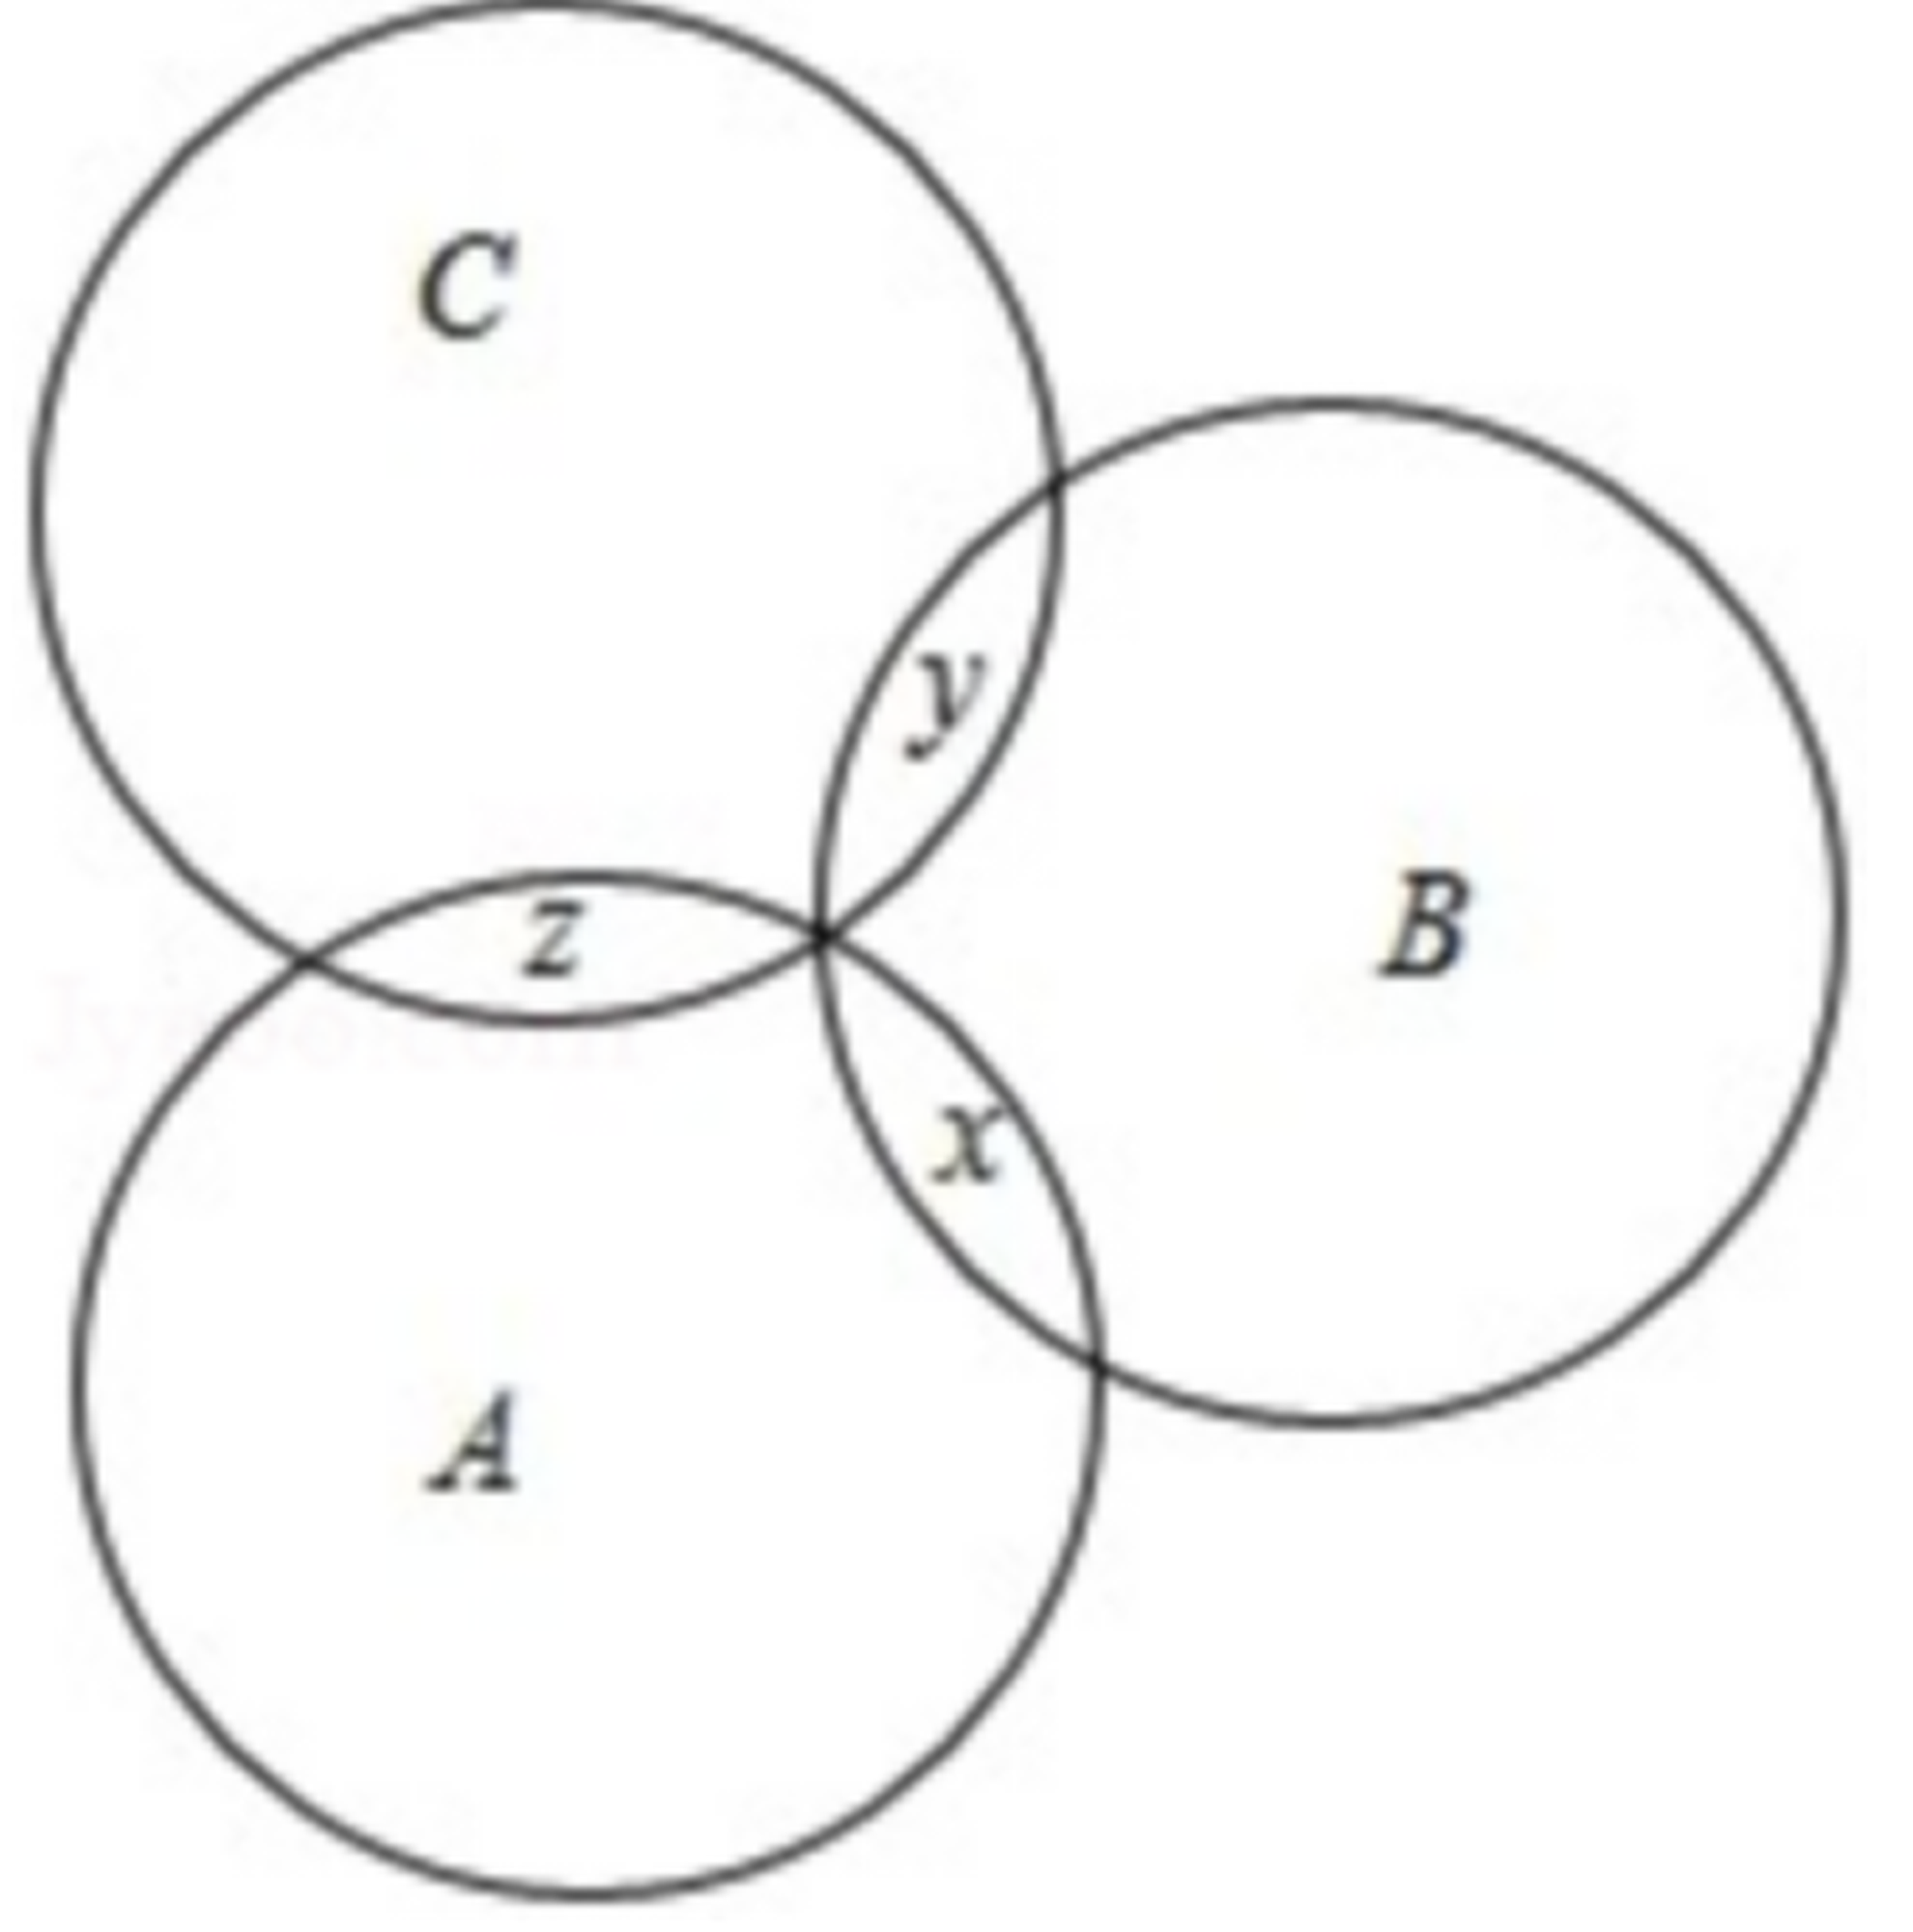
\includegraphics[width=0.30\textwidth]{figures/venn_ABC_x_y_z_h39.png}
\end{center}
\step{因为 $|A\cap B|=|B\cap C|=|C\cap A|=1$，且 $x$、$y$、$z\in\{1,2,3\}$，}
\step{所以集合 $A=\{x,z\}$，$B=\{x,y\}$，$C=\{z,y\}$，}
\step{若 $x=1$，$y=2$，$z=3$，则 $A=\{1,3\}$，$B=\{1,3\}$，$C=\{2,3\}$，}
\step{将 $1$，$2$，$3$ 进行全排列，有 $P_3^3=3\times2=6$ 个.}
\solend

\fi

\item 已知集合 $T=\{1,2,\cdots,2025\}$，对于 $T$ 的每一个非空子集的所有元素，计算它们乘积的倒数，
则所有这样倒数的和为 \blankline[4.4em].

\ans{$2025$}

\ifanswer
\solbegin
\step{集合 $T=\{1,2,\cdots,2025\}$ 的非空子集的个数为 $2^{2025}-1$，}
\step{这些子集中，每个元素的乘积分别为}
\step{$1,2,3,\cdots,2025,1\times2,1\times3,\cdots,1\times2025,\cdots,1\times2\times3\times\cdots\times2025$，}
\step{每项都可以看作是从 $1,2,3,\cdots,2025$ 中选择若干项的乘积，}
\step{$1+\dfrac12+\cdots+\dfrac{1}{2025}+\dfrac{1}{1\times2}+\dfrac{1}{1\times3}+\cdots+\dfrac{1}{2024\times2025}
+\cdots+\dfrac{1}{1\times2\times\cdots\times2025}$}
\step{$=(1+1)\left(1+\dfrac12\right)\cdots\left(1+\dfrac{1}{2025}\right)-1
=2\times\dfrac32\times\dfrac43\times\cdots\times\dfrac{2026}{2025}-1=2025$.}
\solend

\fi

% 第 24 题是压轴题，题干较长；试卷版在它之前量一次页高，尽量不与前文分家（照全稿成例）。
\ansneed{5cm}
% 注：原卷【解析】①③ 两步把 $f(x)$ 印作 $f[x[x]]$，显系笔误，照录未改，见文件头「笔误/存疑」⑦。
\item 若 $X$ 是一个集合，$T$ 是一个以 $X$ 的某些子集为元素的集合，且满足：①$X$ 属于 $T$，
$\varnothing$ 属于 $T$；②$T$ 中任意多个元素的并集属于 $T$；③$T$ 中任意多个元素的交集属于 $T$.
则称 $T$ 是集合 $X$ 上的一个拓扑. 已知函数 $f(x)=[x[x]]$，其中 $[x]$ 表示不大于 $x$ 的最大整数，
当 $x\in(0,n]$，$n\in\N^*$ 时，函数 $f(x)$ 值域为集合 $A_n$，则集合 $A_2$ 上的含有 $4$ 个元素的
拓扑 $T$ 的个数为 \blankline[4.4em].

\ans{$9$}

\ifanswer
\solbegin
\step{由题意，$n=2$，故 $0<x\leqslant2$，}
\step{①当 $0<x<1$ 时，则 $[x]=0$，所以 $f[x[x]]=0$，}
\step{②当 $x=1$ 时，$[x]=1$ 显然 $f(1)=1$，}
\step{③当 $1<x<2$ 时，$[x]=1$，所以 $f[x[x]]=[x]=1$，}
\step{④当 $x=2$ 时，$f(2)=4$，}
\step{所以 $A_2=\{0,1,4\}$，}
\step{因为 $T$ 中含有 $4$ 个元素，其中两个元素 $\varnothing$ 和 $A_2$，}
\step{$A_2=\{0,1,4\}$. 其它两个元素为 $A$、$B$，则
$\begin{cases}A\neq\varnothing\\ A\neq A_2\\ B\neq\varnothing\\ B\neq A_2\\ A\neq B\end{cases}$，}
\step{由对称性，不妨设 $1\leqslant|A|\leqslant|B|\leqslant2$，其中 $|A|$、$|B|$ 表示集合 $A$ 中元素的个数，}
\step{因为 $\begin{cases}A\cap B\in T\\ A\cup B\in T\end{cases}$，又 $|A|\leqslant|B|$，所以 $A\cap B=\varnothing$ 或 $A$，}
\step{若 $A\cap B=\varnothing$，则 $A\cup B$ 只能等于 $A_2$，}
\step{（若 $A\cup B=B$，则 $A\sub B$，则 $A\cap B=A=\varnothing$，矛盾）}
\step{则必有 $\begin{cases}|A|=1\\ |B|=2\end{cases}$，所以 $(A,B)$ 的个数 $\Leftrightarrow$ $A$ 的个数 $=3$ 种，}
\step{即 $\begin{cases}A=\{0\}\\ B=\{1,4\}\end{cases}$ 或 $\begin{cases}A=\{1\}\\ B=\{0,4\}\end{cases}$
或 $\begin{cases}A=\{4\}\\ B=\{0,1\}\end{cases}$；}
\step{若 $A\cap B=A\Leftrightarrow A\sub B$ 此时满足 $A\cup B=B$，}
\step{因为 $A\neq B$ 且 $1\leqslant|A|$ 且 $|B|\leqslant2$，所以 $\begin{cases}|A|=1\\ |B|=2\end{cases}$，}
\step{所以 $B$ 的选择共有 $C_3^2=3$ 种，则 $A$ 的个数有 $C_2^1$ 种，}
\step{所以 $(A,B)$ 的个数 $=2\times3=6$ 种.}
% 这六组「$A$／$B$」按原卷排作两行（前五个一行、第六个另起一行）；因五组并排时
% amsmath 的 cases 会为每组的第二列各留一枚 \quad，本行改排 \left\{\begin{matrix}…\end{matrix}\right.
% 以省下这枚 \quad（照 README「说明」记的高一07 成例），字形与 cases 相同。
\step{（这 $6$ 种是 $\left\{\begin{matrix}A=\{0\}\\ B=\{0,1\}\end{matrix}\right.$、
$\left\{\begin{matrix}A=\{1\}\\ B=\{0,1\}\end{matrix}\right.$、
$\left\{\begin{matrix}A=\{0\}\\ B=\{0,4\}\end{matrix}\right.$、
$\left\{\begin{matrix}A=\{4\}\\ B=\{0,4\}\end{matrix}\right.$、
$\left\{\begin{matrix}A=\{1\}\\ B=\{1,4\}\end{matrix}\right.$、}
\step{$\left\{\begin{matrix}A=\{4\}\\ B=\{1,4\}\end{matrix}\right.$）.}
\step{综上，$T$ 的个数为 $9$ 个.}
\solend

\fi

\end{enumerate}

\end{document}
